\documentclass[a4paper]{book}
\usepackage{a4wide}
\usepackage{makeidx}
\usepackage{fancyhdr}
\usepackage{graphicx}
\usepackage{multicol}
\usepackage{float}
\usepackage{textcomp}
\usepackage{alltt}
\usepackage[utf8]{inputenc}
\usepackage{doxygen}
\makeindex
\setcounter{tocdepth}{1}
\renewcommand{\footrulewidth}{0.4pt}
\begin{document}
\begin{titlepage}
\vspace*{7cm}
\begin{center}
{\Large NFsim Reference Manual\\[1ex]\large 1.01 }\\
\vspace*{1cm}
{\large Generated by Doxygen 1.5.4}\\
\vspace*{0.5cm}
{\small Tue Nov 18 18:05:51 2008}\\
\end{center}
\end{titlepage}
\clearemptydoublepage
\pagenumbering{roman}
\tableofcontents
\clearemptydoublepage
\pagenumbering{arabic}
\chapter{NFsim: The Network Free Stochastic Simulator }
\label{index}\section{Overview}\label{index_intro_sec}
NFsim is a generalized stochastic reaction network simulator designed to handle systems with a large (or even infinite) state space. It has a number of features that make it ideal for handling large and complex biochemical systems, such as functionally defined rate laws and reactions that depend on local context. NFsim is designed to operate with the BioNetGen Language ({\tt http://bionetgen.org/}). The new version of BNG is able to generate an XML encoded form of the BNG Language, which NFsim can take as input.

For more details on setting up, running, and getting output from an NFsim simulation see the User Manual. The User Manual also has additional information for new developers. The manual is available online along with examples here: {\tt http://emonet.biology.yale.edu/nfsim}\section{Command Line Argument List}\label{index_key}
Arguments can be provided to NFsim through the command line. Below is a partial list of the available commands and a brief description of what they do. For more details, see the NFsim user manual.

-help = outputs a helpful message to the console

-xml [filename] = specifies the xml file to read

-sim [Duration in sec] = specifies the length of time to simulate the system

-oSteps [num of steps] = specifies the number of times to output during the simulation

-eq [Duration in sec] = specifies the length of time to equilibrate before simulating

-o [filename] = specifies the name of the output file

-v = verbose output when reading an xml file and building a system

-b = output in binary (faster, but output is not human readable)

-utl [integer] = universal traversal limit, see manual

-notf = disables On the Fly Observables, see manual

-cb = turn on complex bookkeeping, see manual

-gml [integer] = sets maximal number of molecules, per any MoleculeType, see manual\section{Developers}\label{index_devel_sec}
To begin developing and extending NFsim, the best place to start looking is in the src/NFtest/simple\_\-system directory. Here you'll find two files, \doxyref{simple\_\-system.hh}{p.}{simple__system_8hh} and \doxyref{simple\_\-system.cpp}{p.}{simple__system_8cpp}. Together, this code specifies a simple enzymatic type reaction that is completely hard coded. This will give you an idea of the basic classes and functions used to define, initialize, run, and output a simulation. From there, you can dive into the specific classes and functions that you need to work with. Details about how to run the simple\_\-system example are given in these files.

All of the other main classes are defined in the \doxyref{NFcore}{p.}{namespaceNFcore} namespace and are found in the \doxyref{NFcore}{p.}{namespaceNFcore} directory and the NFreactions directory. The \doxyref{NFcore}{p.}{namespaceNFcore} directory contains the basic structure of the simulation engine while the NFreactions directory contains the classes associated with actually executing rules and transforming molecules. \doxyref{NFinput}{p.}{namespaceNFinput} contains what's needed for the xml parser (built using the TinyXML package) and the command line parser. \doxyref{NFutil}{p.}{namespaceNFutil} also contains a nice implementation of the Mersenne Twister random number generator which should be used for all random number generation in NFsim. NFoutput is more sparse as it deals only with handling the more complicated output required of groups and complexes. (Basic outputting is handled easily with the System and Observable classes in the \doxyref{NFcore}{p.}{namespaceNFcore} namespace).

Another note for developers: class functions and member variables are generally well commented in the header file in which they are declared. So if you are lost in some source file, and you think there aren't any comments, be sure to check the header file before you ask for help.\section{Authors \& Acknowledgments}\label{index_author_sec}
The NFsim code was written and developed by Michael Sneddon with help from James Faeder and Thierry Emonet. James Faeder wrote the extended BioNetGen code that can output XML encodings of the BNGL.

A number of other people have helped in getting NFsim to where it is today, either by aiding in the concepts of the design, testing the implementation, adding some features to the code, or by suggesting improvements.

A partial list of these people include:

Garrit Jentsch, William Pontius, Oleksii Sliusarenko, Justin Hogg, Christopher Henry, Fangfang Xia, Ryan Gutenkunst, 
\chapter{NFsim Namespace Index}
\section{NFsim Namespace List}
Here is a list of all namespaces with brief descriptions:\begin{CompactList}
\item\contentsline{section}{{\bf mu} }{\pageref{namespacemu}}{}
\item\contentsline{section}{{\bf NFcore} (Contains the primary classes and functions of NFsim )}{\pageref{namespaceNFcore}}{}
\item\contentsline{section}{{\bf NFinput} (Functionality to handle input from XML files or command line arguments )}{\pageref{namespaceNFinput}}{}
\item\contentsline{section}{{\bf NFtest\_\-ss} (Namespace for the Simple System (abreviated ss) example )}{\pageref{namespaceNFtest__ss}}{}
\item\contentsline{section}{{\bf NFtest\_\-tlbr} (Tests for running the TLBR system )}{\pageref{namespaceNFtest__tlbr}}{}
\item\contentsline{section}{{\bf NFtest\_\-transcription} (Namespace for the Transcription example )}{\pageref{namespaceNFtest__transcription}}{}
\item\contentsline{section}{{\bf NFutil} (General utility functions for NFsim, including a random number generator and a function parser )}{\pageref{namespaceNFutil}}{}
\item\contentsline{section}{{\bf std} }{\pageref{namespacestd}}{}
\end{CompactList}

\chapter{NFsim Hierarchical Index}
\section{NFsim Class Hierarchy}
This inheritance list is sorted roughly, but not completely, alphabetically:\begin{CompactList}
\item \contentsline{section}{AgentCell}{\pageref{classAgentCell}}{}
\item \contentsline{section}{NFcore::Complex}{\pageref{classNFcore_1_1Complex}}{}
\item \contentsline{section}{NFcore::ComplexList}{\pageref{classNFcore_1_1ComplexList}}{}
\item \contentsline{section}{NFinput::component}{\pageref{classNFinput_1_1component}}{}
\item \contentsline{section}{NFcore::CompositeFunction}{\pageref{classNFcore_1_1CompositeFunction}}{}
\item \contentsline{section}{NFcore::DumpSystem}{\pageref{classNFcore_1_1DumpSystem}}{}
\item \contentsline{section}{Environment}{\pageref{classEnvironment}}{}
\begin{CompactList}
\item \contentsline{section}{ConstantEnvironment}{\pageref{classConstantEnvironment}}{}
\item \contentsline{section}{LinearEnvironment}{\pageref{classLinearEnvironment}}{}
\end{CompactList}
\item \contentsline{section}{NFcore::FuncFactory}{\pageref{classNFcore_1_1FuncFactory}}{}
\item \contentsline{section}{NFcore::FunctionReference}{\pageref{classNFcore_1_1FunctionReference}}{}
\item \contentsline{section}{ChemotaxisUtil::GammaSampler}{\pageref{classChemotaxisUtil_1_1GammaSampler}}{}
\item \contentsline{section}{NFcore::GlobalFunction}{\pageref{classNFcore_1_1GlobalFunction}}{}
\item \contentsline{section}{IsInWrongComplex}{\pageref{classIsInWrongComplex}}{}
\item \contentsline{section}{job}{\pageref{structjob}}{}
\item \contentsline{section}{NFcore::LocalFunction}{\pageref{classNFcore_1_1LocalFunction}}{}
\item \contentsline{section}{NFcore::MapGenerator}{\pageref{classNFcore_1_1MapGenerator}}{}
\item \contentsline{section}{NFcore::Mapping}{\pageref{classNFcore_1_1Mapping}}{}
\item \contentsline{section}{NFcore::MappingSet}{\pageref{classNFcore_1_1MappingSet}}{}
\item \contentsline{section}{model}{\pageref{structmodel}}{}
\item \contentsline{section}{NFcore::Molecule}{\pageref{classNFcore_1_1Molecule}}{}
\item \contentsline{section}{NFcore::MoleculeList}{\pageref{classNFcore_1_1MoleculeList}}{}
\item \contentsline{section}{NFcore::MoleculeType}{\pageref{classNFcore_1_1MoleculeType}}{}
\item \contentsline{section}{msgtype}{\pageref{structmsgtype}}{}
\item \contentsline{section}{MTRand\_\-int32}{\pageref{classMTRand__int32}}{}
\begin{CompactList}
\item \contentsline{section}{MTRand}{\pageref{classMTRand}}{}
\item \contentsline{section}{MTRand53}{\pageref{classMTRand53}}{}
\item \contentsline{section}{MTRand\_\-closed}{\pageref{classMTRand__closed}}{}
\item \contentsline{section}{MTRand\_\-open}{\pageref{classMTRand__open}}{}
\end{CompactList}
\item \contentsline{section}{NFstream}{\pageref{classNFstream}}{}
\item \contentsline{section}{NFcore::Observable}{\pageref{classNFcore_1_1Observable}}{}
\begin{CompactList}
\item \contentsline{section}{NFcore::MoleculesObservable}{\pageref{classNFcore_1_1MoleculesObservable}}{}
\item \contentsline{section}{NFcore::SpeciesObservable}{\pageref{classNFcore_1_1SpeciesObservable}}{}
\end{CompactList}
\item \contentsline{section}{NFcore::Outputter}{\pageref{classNFcore_1_1Outputter}}{}
\item \contentsline{section}{NFcore::ReactantContainer}{\pageref{classNFcore_1_1ReactantContainer}}{}
\begin{CompactList}
\item \contentsline{section}{NFcore::ReactantList}{\pageref{classNFcore_1_1ReactantList}}{}
\item \contentsline{section}{NFcore::ReactantTree}{\pageref{classNFcore_1_1ReactantTree}}{}
\end{CompactList}
\item \contentsline{section}{NFcore::ReactionClass}{\pageref{classNFcore_1_1ReactionClass}}{}
\begin{CompactList}
\item \contentsline{section}{NFcore::BasicRxnClass}{\pageref{classNFcore_1_1BasicRxnClass}}{}
\begin{CompactList}
\item \contentsline{section}{NFcore::FunctionalRxnClass}{\pageref{classNFcore_1_1FunctionalRxnClass}}{}
\item \contentsline{section}{NFcore::MMRxnClass}{\pageref{classNFcore_1_1MMRxnClass}}{}
\end{CompactList}
\item \contentsline{section}{NFcore::DORRxnClass}{\pageref{classNFcore_1_1DORRxnClass}}{}
\end{CompactList}
\item \contentsline{section}{NFcore::ReactionSelector}{\pageref{classNFcore_1_1ReactionSelector}}{}
\begin{CompactList}
\item \contentsline{section}{NFcore::DirectSelector}{\pageref{classNFcore_1_1DirectSelector}}{}
\item \contentsline{section}{NFcore::LogClassSelector}{\pageref{classNFcore_1_1LogClassSelector}}{}
\end{CompactList}
\item \contentsline{section}{scan}{\pageref{structscan}}{}
\item \contentsline{section}{NFcore::SpeciesCreator}{\pageref{classNFcore_1_1SpeciesCreator}}{}
\item \contentsline{section}{NFcore::StateCounter}{\pageref{classNFcore_1_1StateCounter}}{}
\item \contentsline{section}{NFcore::System}{\pageref{classNFcore_1_1System}}{}
\item \contentsline{section}{NFcore::TemplateMolecule}{\pageref{classNFcore_1_1TemplateMolecule}}{}
\item \contentsline{section}{TiXmlAttributeSet}{\pageref{classTiXmlAttributeSet}}{}
\item \contentsline{section}{TiXmlBase}{\pageref{classTiXmlBase}}{}
\begin{CompactList}
\item \contentsline{section}{TiXmlAttribute}{\pageref{classTiXmlAttribute}}{}
\item \contentsline{section}{TiXmlNode}{\pageref{classTiXmlNode}}{}
\begin{CompactList}
\item \contentsline{section}{TiXmlComment}{\pageref{classTiXmlComment}}{}
\item \contentsline{section}{TiXmlDeclaration}{\pageref{classTiXmlDeclaration}}{}
\item \contentsline{section}{TiXmlDocument}{\pageref{classTiXmlDocument}}{}
\item \contentsline{section}{TiXmlElement}{\pageref{classTiXmlElement}}{}
\item \contentsline{section}{TiXmlText}{\pageref{classTiXmlText}}{}
\item \contentsline{section}{TiXmlUnknown}{\pageref{classTiXmlUnknown}}{}
\end{CompactList}
\end{CompactList}
\item \contentsline{section}{TiXmlCursor}{\pageref{structTiXmlCursor}}{}
\item \contentsline{section}{TiXmlHandle}{\pageref{classTiXmlHandle}}{}
\item \contentsline{section}{TiXmlParsingData}{\pageref{classTiXmlParsingData}}{}
\item \contentsline{section}{TiXmlString}{\pageref{classTiXmlString}}{}
\begin{CompactList}
\item \contentsline{section}{TiXmlOutStream}{\pageref{classTiXmlOutStream}}{}
\end{CompactList}
\item \contentsline{section}{TiXmlVisitor}{\pageref{classTiXmlVisitor}}{}
\begin{CompactList}
\item \contentsline{section}{TiXmlPrinter}{\pageref{classTiXmlPrinter}}{}
\end{CompactList}
\item \contentsline{section}{NFcore::Transformation}{\pageref{classNFcore_1_1Transformation}}{}
\begin{CompactList}
\item \contentsline{section}{NFcore::AddMoleculeTransform}{\pageref{classNFcore_1_1AddMoleculeTransform}}{}
\item \contentsline{section}{NFcore::BindingTransform}{\pageref{classNFcore_1_1BindingTransform}}{}
\begin{CompactList}
\item \contentsline{section}{NFcore::BindingSeparateComplexTransform}{\pageref{classNFcore_1_1BindingSeparateComplexTransform}}{}
\end{CompactList}
\item \contentsline{section}{NFcore::DecrementStateTransform}{\pageref{classNFcore_1_1DecrementStateTransform}}{}
\item \contentsline{section}{NFcore::EmptyTransform}{\pageref{classNFcore_1_1EmptyTransform}}{}
\item \contentsline{section}{NFcore::IncrementStateTransform}{\pageref{classNFcore_1_1IncrementStateTransform}}{}
\item \contentsline{section}{NFcore::LocalFunctionReference}{\pageref{classNFcore_1_1LocalFunctionReference}}{}
\item \contentsline{section}{NFcore::RemoveMoleculeTransform}{\pageref{classNFcore_1_1RemoveMoleculeTransform}}{}
\item \contentsline{section}{NFcore::StateChangeTransform}{\pageref{classNFcore_1_1StateChangeTransform}}{}
\item \contentsline{section}{NFcore::UnbindingTransform}{\pageref{classNFcore_1_1UnbindingTransform}}{}
\end{CompactList}
\item \contentsline{section}{NFcore::TransformationFactory}{\pageref{classNFcore_1_1TransformationFactory}}{}
\item \contentsline{section}{NFcore::TransformationSet}{\pageref{classNFcore_1_1TransformationSet}}{}
\end{CompactList}

\chapter{NFsim Class Index}
\section{NFsim Class List}
Here are the classes, structs, unions and interfaces with brief descriptions:\begin{CompactList}
\item\contentsline{section}{{\bf NFcore::AddMoleculeTransform} }{\pageref{classNFcore_1_1AddMoleculeTransform}}{}
\item\contentsline{section}{{\bf NFcore::AddSpeciesTransform} }{\pageref{classNFcore_1_1AddSpeciesTransform}}{}
\item\contentsline{section}{{\bf AgentCell} }{\pageref{classAgentCell}}{}
\item\contentsline{section}{{\bf NFcore::BasicRxnClass} }{\pageref{classNFcore_1_1BasicRxnClass}}{}
\item\contentsline{section}{{\bf NFcore::BindingTransform} }{\pageref{classNFcore_1_1BindingTransform}}{}
\item\contentsline{section}{{\bf NFcore::Complex} (Container to dynamically keep track of all system complexes )}{\pageref{classNFcore_1_1Complex}}{}
\item\contentsline{section}{{\bf NFcore::ComplexList} (Container to organize all system complexes )}{\pageref{classNFcore_1_1ComplexList}}{}
\item\contentsline{section}{{\bf NFinput::component} (Maintains information about a \doxyref{component}{p.}{classNFinput_1_1component} of a TemplateMolecule )}{\pageref{classNFinput_1_1component}}{}
\item\contentsline{section}{{\bf NFcore::CompositeFunction} }{\pageref{classNFcore_1_1CompositeFunction}}{}
\item\contentsline{section}{{\bf ConstantEnvironment} }{\pageref{classConstantEnvironment}}{}
\item\contentsline{section}{{\bf NFcore::DecrementPopulationTransform} }{\pageref{classNFcore_1_1DecrementPopulationTransform}}{}
\item\contentsline{section}{{\bf NFcore::DecrementStateTransform} }{\pageref{classNFcore_1_1DecrementStateTransform}}{}
\item\contentsline{section}{{\bf NFcore::DirectSelector} }{\pageref{classNFcore_1_1DirectSelector}}{}
\item\contentsline{section}{{\bf NFcore::DORRxnClass} }{\pageref{classNFcore_1_1DORRxnClass}}{}
\item\contentsline{section}{{\bf NFcore::DumpSystem} (Class for outputting the state of the system )}{\pageref{classNFcore_1_1DumpSystem}}{}
\item\contentsline{section}{{\bf NFcore::EmptyTransform} }{\pageref{classNFcore_1_1EmptyTransform}}{}
\item\contentsline{section}{{\bf Environment} }{\pageref{classEnvironment}}{}
\item\contentsline{section}{{\bf NFcore::FuncFactory} (Parses mathmatical functions that can be easily used anywhere )}{\pageref{classNFcore_1_1FuncFactory}}{}
\item\contentsline{section}{{\bf NFcore::FunctionalRxnClass} }{\pageref{classNFcore_1_1FunctionalRxnClass}}{}
\item\contentsline{section}{{\bf NFcore::FunctionReference} }{\pageref{classNFcore_1_1FunctionReference}}{}
\item\contentsline{section}{{\bf ChemotaxisUtil::GammaSampler} }{\pageref{classChemotaxisUtil_1_1GammaSampler}}{}
\item\contentsline{section}{{\bf NFcore::GlobalFunction} (Defines functions to be used globally in a simulation )}{\pageref{classNFcore_1_1GlobalFunction}}{}
\item\contentsline{section}{{\bf NFcore::IncrementStateTransform} }{\pageref{classNFcore_1_1IncrementStateTransform}}{}
\item\contentsline{section}{{\bf IsInWrongComplex} }{\pageref{classIsInWrongComplex}}{}
\item\contentsline{section}{{\bf job} }{\pageref{structjob}}{}
\item\contentsline{section}{{\bf LinearEnvironment} }{\pageref{classLinearEnvironment}}{}
\item\contentsline{section}{{\bf NFcore::LocalFunction} }{\pageref{classNFcore_1_1LocalFunction}}{}
\item\contentsline{section}{{\bf NFcore::LocalFunctionReference} }{\pageref{classNFcore_1_1LocalFunctionReference}}{}
\item\contentsline{section}{{\bf NFcore::LogClassSelector} }{\pageref{classNFcore_1_1LogClassSelector}}{}
\item\contentsline{section}{{\bf NFcore::MapGenerator} (Knows how to assign mappings in a \doxyref{MappingSet}{p.}{classNFcore_1_1MappingSet} to a particular \doxyref{Molecule}{p.}{classNFcore_1_1Molecule} )}{\pageref{classNFcore_1_1MapGenerator}}{}
\item\contentsline{section}{{\bf NFcore::Mapping} (Keeps a pointer to a molecule and remembers a single component to act on )}{\pageref{classNFcore_1_1Mapping}}{}
\item\contentsline{section}{{\bf NFcore::MappingSet} (Keeps a list of mappings needed by a particular list of reactants )}{\pageref{classNFcore_1_1MappingSet}}{}
\item\contentsline{section}{{\bf NFcore::MMRxnClass} }{\pageref{classNFcore_1_1MMRxnClass}}{}
\item\contentsline{section}{{\bf model} }{\pageref{structmodel}}{}
\item\contentsline{section}{{\bf NFcore::Molecule} (Each molecule in the system is represented by an instance of this )}{\pageref{classNFcore_1_1Molecule}}{}
\item\contentsline{section}{{\bf NFcore::MoleculeCreator} }{\pageref{classNFcore_1_1MoleculeCreator}}{}
\item\contentsline{section}{{\bf NFcore::MoleculeList} (Keeps a set of molecules neatly for a \doxyref{MoleculeType}{p.}{classNFcore_1_1MoleculeType} )}{\pageref{classNFcore_1_1MoleculeList}}{}
\item\contentsline{section}{{\bf NFcore::MoleculesObservable} }{\pageref{classNFcore_1_1MoleculesObservable}}{}
\item\contentsline{section}{{\bf NFcore::MoleculeType} (Keeps track of the types of molecules that can exist )}{\pageref{classNFcore_1_1MoleculeType}}{}
\item\contentsline{section}{{\bf msgtype} }{\pageref{structmsgtype}}{}
\item\contentsline{section}{{\bf MTRand} }{\pageref{classMTRand}}{}
\item\contentsline{section}{{\bf MTRand53} }{\pageref{classMTRand53}}{}
\item\contentsline{section}{{\bf MTRand\_\-closed} }{\pageref{classMTRand__closed}}{}
\item\contentsline{section}{{\bf MTRand\_\-int32} }{\pageref{classMTRand__int32}}{}
\item\contentsline{section}{{\bf MTRand\_\-open} }{\pageref{classMTRand__open}}{}
\item\contentsline{section}{{\bf NFcore::NewMoleculeBindingTransform} }{\pageref{classNFcore_1_1NewMoleculeBindingTransform}}{}
\item\contentsline{section}{{\bf NFstream} }{\pageref{classNFstream}}{}
\item\contentsline{section}{{\bf NFcore::Observable} (Tracks the counts of predefined observables in the simulation )}{\pageref{classNFcore_1_1Observable}}{}
\item\contentsline{section}{{\bf NFcore::Outputter} }{\pageref{classNFcore_1_1Outputter}}{}
\item\contentsline{section}{{\bf NFcore::PopulationRxnClass} }{\pageref{classNFcore_1_1PopulationRxnClass}}{}
\item\contentsline{section}{{\bf NFcore::ReactantContainer} (Interface for all containers of Reactants (MappingSets) needed by ReactionClasses )}{\pageref{classNFcore_1_1ReactantContainer}}{}
\item\contentsline{section}{{\bf NFcore::ReactantList} (Maintains a list of MappingSets needed by \doxyref{ReactionClass}{p.}{classNFcore_1_1ReactionClass} )}{\pageref{classNFcore_1_1ReactantList}}{}
\item\contentsline{section}{{\bf NFcore::ReactantTree} (Maintains a tree of MappingSets needed by Distribution of Rates Reactions )}{\pageref{classNFcore_1_1ReactantTree}}{}
\item\contentsline{section}{{\bf NFcore::ReactionClass} (Abstract Base Class that defines the interface for all reaction rules )}{\pageref{classNFcore_1_1ReactionClass}}{}
\item\contentsline{section}{{\bf NFcore::ReactionSelector} }{\pageref{classNFcore_1_1ReactionSelector}}{}
\item\contentsline{section}{{\bf NFcore::RemoveMoleculeTransform} }{\pageref{classNFcore_1_1RemoveMoleculeTransform}}{}
\item\contentsline{section}{{\bf scan} }{\pageref{structscan}}{}
\item\contentsline{section}{{\bf NFcore::SpeciesCreator} }{\pageref{classNFcore_1_1SpeciesCreator}}{}
\item\contentsline{section}{{\bf NFcore::SpeciesObservable} }{\pageref{classNFcore_1_1SpeciesObservable}}{}
\item\contentsline{section}{{\bf NFcore::StateChangeTransform} }{\pageref{classNFcore_1_1StateChangeTransform}}{}
\item\contentsline{section}{{\bf NFcore::StateCounter} }{\pageref{classNFcore_1_1StateCounter}}{}
\item\contentsline{section}{{\bf NFcore::System} (The main class that begins and runs simulations )}{\pageref{classNFcore_1_1System}}{}
\item\contentsline{section}{{\bf NFcore::TemplateMolecule} (Used for matching \doxyref{Molecule}{p.}{classNFcore_1_1Molecule} objects to the given pattern )}{\pageref{classNFcore_1_1TemplateMolecule}}{}
\item\contentsline{section}{{\bf TiXmlAttribute} }{\pageref{classTiXmlAttribute}}{}
\item\contentsline{section}{{\bf TiXmlAttributeSet} }{\pageref{classTiXmlAttributeSet}}{}
\item\contentsline{section}{{\bf TiXmlBase} }{\pageref{classTiXmlBase}}{}
\item\contentsline{section}{{\bf TiXmlComment} }{\pageref{classTiXmlComment}}{}
\item\contentsline{section}{{\bf TiXmlCursor} }{\pageref{structTiXmlCursor}}{}
\item\contentsline{section}{{\bf TiXmlDeclaration} }{\pageref{classTiXmlDeclaration}}{}
\item\contentsline{section}{{\bf TiXmlDocument} }{\pageref{classTiXmlDocument}}{}
\item\contentsline{section}{{\bf TiXmlElement} }{\pageref{classTiXmlElement}}{}
\item\contentsline{section}{{\bf TiXmlHandle} }{\pageref{classTiXmlHandle}}{}
\item\contentsline{section}{{\bf TiXmlNode} }{\pageref{classTiXmlNode}}{}
\item\contentsline{section}{{\bf TiXmlOutStream} }{\pageref{classTiXmlOutStream}}{}
\item\contentsline{section}{{\bf TiXmlParsingData} }{\pageref{classTiXmlParsingData}}{}
\item\contentsline{section}{{\bf TiXmlPrinter} }{\pageref{classTiXmlPrinter}}{}
\item\contentsline{section}{{\bf TiXmlString} }{\pageref{classTiXmlString}}{}
\item\contentsline{section}{{\bf TiXmlText} }{\pageref{classTiXmlText}}{}
\item\contentsline{section}{{\bf TiXmlUnknown} }{\pageref{classTiXmlUnknown}}{}
\item\contentsline{section}{{\bf TiXmlVisitor} }{\pageref{classTiXmlVisitor}}{}
\item\contentsline{section}{{\bf NFcore::Transformation} }{\pageref{classNFcore_1_1Transformation}}{}
\item\contentsline{section}{{\bf NFcore::TransformationFactory} }{\pageref{classNFcore_1_1TransformationFactory}}{}
\item\contentsline{section}{{\bf NFcore::TransformationSet} (Maintains a set of \doxyref{Transformation}{p.}{classNFcore_1_1Transformation} objects for a \doxyref{ReactionClass}{p.}{classNFcore_1_1ReactionClass} )}{\pageref{classNFcore_1_1TransformationSet}}{}
\item\contentsline{section}{{\bf NFcore::UnbindingTransform} }{\pageref{classNFcore_1_1UnbindingTransform}}{}
\end{CompactList}

\chapter{NFsim File Index}
\section{NFsim File List}
Here is a list of all files with brief descriptions:\begin{CompactList}
\item\contentsline{section}{/home/msneddon/eclipse/indigo/workspace/NFsim/src/{\bf NFsim.cpp} }{\pageref{NFsim_8cpp}}{}
\item\contentsline{section}{/home/msneddon/eclipse/indigo/workspace/NFsim/src/{\bf NFsim.hh} }{\pageref{NFsim_8hh}}{}
\item\contentsline{section}{/home/msneddon/eclipse/indigo/workspace/NFsim/src/NFcore/{\bf complex.cpp} }{\pageref{complex_8cpp}}{}
\item\contentsline{section}{/home/msneddon/eclipse/indigo/workspace/NFsim/src/NFcore/{\bf complexList.cpp} }{\pageref{complexList_8cpp}}{}
\item\contentsline{section}{/home/msneddon/eclipse/indigo/workspace/NFsim/src/NFcore/{\bf molecule.cpp} }{\pageref{molecule_8cpp}}{}
\item\contentsline{section}{/home/msneddon/eclipse/indigo/workspace/NFsim/src/NFcore/{\bf moleculeType.cpp} }{\pageref{moleculeType_8cpp}}{}
\item\contentsline{section}{/home/msneddon/eclipse/indigo/workspace/NFsim/src/NFcore/{\bf NFcore.hh} (Contains declarations of core NFsim classes )}{\pageref{NFcore_8hh}}{}
\item\contentsline{section}{/home/msneddon/eclipse/indigo/workspace/NFsim/src/NFcore/{\bf observable.cpp} }{\pageref{observable_8cpp}}{}
\item\contentsline{section}{/home/msneddon/eclipse/indigo/workspace/NFsim/src/NFcore/{\bf observable.hh} }{\pageref{observable_8hh}}{}
\item\contentsline{section}{/home/msneddon/eclipse/indigo/workspace/NFsim/src/NFcore/{\bf reactionClass.cpp} }{\pageref{reactionClass_8cpp}}{}
\item\contentsline{section}{/home/msneddon/eclipse/indigo/workspace/NFsim/src/NFcore/{\bf system.cpp} }{\pageref{system_8cpp}}{}
\item\contentsline{section}{/home/msneddon/eclipse/indigo/workspace/NFsim/src/NFcore/{\bf templateMolecule.cpp} }{\pageref{templateMolecule_8cpp}}{}
\item\contentsline{section}{/home/msneddon/eclipse/indigo/workspace/NFsim/src/NFcore/{\bf templateMolecule.hh} }{\pageref{templateMolecule_8hh}}{}
\item\contentsline{section}{/home/msneddon/eclipse/indigo/workspace/NFsim/src/NFcore/moleculeLists/{\bf moleculeList.cpp} }{\pageref{moleculeList_8cpp}}{}
\item\contentsline{section}{/home/msneddon/eclipse/indigo/workspace/NFsim/src/NFcore/moleculeLists/{\bf moleculeList.hh} }{\pageref{moleculeList_8hh}}{}
\item\contentsline{section}{/home/msneddon/eclipse/indigo/workspace/NFsim/src/NFcore/reactionSelector/{\bf directSelector.cpp} }{\pageref{directSelector_8cpp}}{}
\item\contentsline{section}{/home/msneddon/eclipse/indigo/workspace/NFsim/src/NFcore/reactionSelector/{\bf logClassSelector.cpp} }{\pageref{logClassSelector_8cpp}}{}
\item\contentsline{section}{/home/msneddon/eclipse/indigo/workspace/NFsim/src/NFcore/reactionSelector/{\bf reactionSelector.hh} }{\pageref{reactionSelector_8hh}}{}
\item\contentsline{section}{/home/msneddon/eclipse/indigo/workspace/NFsim/src/NFfunction/{\bf compositeFunction.cpp} }{\pageref{compositeFunction_8cpp}}{}
\item\contentsline{section}{/home/msneddon/eclipse/indigo/workspace/NFsim/src/NFfunction/{\bf funcParser.cpp} }{\pageref{funcParser_8cpp}}{}
\item\contentsline{section}{/home/msneddon/eclipse/indigo/workspace/NFsim/src/NFfunction/{\bf function.cpp} }{\pageref{function_8cpp}}{}
\item\contentsline{section}{/home/msneddon/eclipse/indigo/workspace/NFsim/src/NFfunction/{\bf localFunction.cpp} }{\pageref{localFunction_8cpp}}{}
\item\contentsline{section}{/home/msneddon/eclipse/indigo/workspace/NFsim/src/NFfunction/{\bf NFfunction.hh} }{\pageref{NFfunction_8hh}}{}
\item\contentsline{section}{/home/msneddon/eclipse/indigo/workspace/NFsim/src/NFinput/{\bf commandLineParser.cpp} }{\pageref{commandLineParser_8cpp}}{}
\item\contentsline{section}{/home/msneddon/eclipse/indigo/workspace/NFsim/src/NFinput/{\bf NFinput.cpp} }{\pageref{NFinput_8cpp}}{}
\item\contentsline{section}{/home/msneddon/eclipse/indigo/workspace/NFsim/src/NFinput/{\bf NFinput.hh} }{\pageref{NFinput_8hh}}{}
\item\contentsline{section}{/home/msneddon/eclipse/indigo/workspace/NFsim/src/NFinput/{\bf parseFuncXML.cpp} }{\pageref{parseFuncXML_8cpp}}{}
\item\contentsline{section}{/home/msneddon/eclipse/indigo/workspace/NFsim/src/NFinput/{\bf parseSymRxns.cpp} }{\pageref{parseSymRxns_8cpp}}{}
\item\contentsline{section}{/home/msneddon/eclipse/indigo/workspace/NFsim/src/NFinput/{\bf rnfRunner.cpp} }{\pageref{rnfRunner_8cpp}}{}
\item\contentsline{section}{/home/msneddon/eclipse/indigo/workspace/NFsim/src/NFinput/{\bf walk.cpp} }{\pageref{walk_8cpp}}{}
\item\contentsline{section}{/home/msneddon/eclipse/indigo/workspace/NFsim/src/NFinput/TinyXML/{\bf tinystr.cpp} }{\pageref{tinystr_8cpp}}{}
\item\contentsline{section}{/home/msneddon/eclipse/indigo/workspace/NFsim/src/NFinput/TinyXML/{\bf tinystr.h} }{\pageref{tinystr_8h}}{}
\item\contentsline{section}{/home/msneddon/eclipse/indigo/workspace/NFsim/src/NFinput/TinyXML/{\bf tinyxml.cpp} }{\pageref{tinyxml_8cpp}}{}
\item\contentsline{section}{/home/msneddon/eclipse/indigo/workspace/NFsim/src/NFinput/TinyXML/{\bf tinyxml.h} }{\pageref{tinyxml_8h}}{}
\item\contentsline{section}{/home/msneddon/eclipse/indigo/workspace/NFsim/src/NFinput/TinyXML/{\bf tinyxmlerror.cpp} }{\pageref{tinyxmlerror_8cpp}}{}
\item\contentsline{section}{/home/msneddon/eclipse/indigo/workspace/NFsim/src/NFinput/TinyXML/{\bf tinyxmlparser.cpp} }{\pageref{tinyxmlparser_8cpp}}{}
\item\contentsline{section}{/home/msneddon/eclipse/indigo/workspace/NFsim/src/NFoutput/{\bf NFoutput.cpp} }{\pageref{NFoutput_8cpp}}{}
\item\contentsline{section}{/home/msneddon/eclipse/indigo/workspace/NFsim/src/NFoutput/{\bf NFoutput.hh} }{\pageref{NFoutput_8hh}}{}
\item\contentsline{section}{/home/msneddon/eclipse/indigo/workspace/NFsim/src/NFreactions/{\bf NFreactions.cpp} }{\pageref{NFreactions_8cpp}}{}
\item\contentsline{section}{/home/msneddon/eclipse/indigo/workspace/NFsim/src/NFreactions/{\bf NFreactions.hh} }{\pageref{NFreactions_8hh}}{}
\item\contentsline{section}{/home/msneddon/eclipse/indigo/workspace/NFsim/src/NFreactions/mappings/{\bf mapping.cpp} }{\pageref{mapping_8cpp}}{}
\item\contentsline{section}{/home/msneddon/eclipse/indigo/workspace/NFsim/src/NFreactions/mappings/{\bf mapping.hh} }{\pageref{mapping_8hh}}{}
\item\contentsline{section}{/home/msneddon/eclipse/indigo/workspace/NFsim/src/NFreactions/mappings/{\bf mappingGenerator.cpp} }{\pageref{mappingGenerator_8cpp}}{}
\item\contentsline{section}{/home/msneddon/eclipse/indigo/workspace/NFsim/src/NFreactions/mappings/{\bf mappingGenerator.hh} }{\pageref{mappingGenerator_8hh}}{}
\item\contentsline{section}{/home/msneddon/eclipse/indigo/workspace/NFsim/src/NFreactions/mappings/{\bf mappingSet.cpp} }{\pageref{mappingSet_8cpp}}{}
\item\contentsline{section}{/home/msneddon/eclipse/indigo/workspace/NFsim/src/NFreactions/mappings/{\bf mappingSet.hh} }{\pageref{mappingSet_8hh}}{}
\item\contentsline{section}{/home/msneddon/eclipse/indigo/workspace/NFsim/src/NFreactions/reactantLists/{\bf reactantContainer.hh} }{\pageref{reactantContainer_8hh}}{}
\item\contentsline{section}{/home/msneddon/eclipse/indigo/workspace/NFsim/src/NFreactions/reactantLists/{\bf reactantList.cpp} }{\pageref{reactantList_8cpp}}{}
\item\contentsline{section}{/home/msneddon/eclipse/indigo/workspace/NFsim/src/NFreactions/reactantLists/{\bf reactantList.hh} }{\pageref{reactantList_8hh}}{}
\item\contentsline{section}{/home/msneddon/eclipse/indigo/workspace/NFsim/src/NFreactions/reactantLists/{\bf reactantTree.cpp} }{\pageref{reactantTree_8cpp}}{}
\item\contentsline{section}{/home/msneddon/eclipse/indigo/workspace/NFsim/src/NFreactions/reactantLists/{\bf reactantTree.hh} }{\pageref{reactantTree_8hh}}{}
\item\contentsline{section}{/home/msneddon/eclipse/indigo/workspace/NFsim/src/NFreactions/reactions/{\bf DORreaction.cpp} }{\pageref{DORreaction_8cpp}}{}
\item\contentsline{section}{/home/msneddon/eclipse/indigo/workspace/NFsim/src/NFreactions/reactions/{\bf reaction.cpp} }{\pageref{reaction_8cpp}}{}
\item\contentsline{section}{/home/msneddon/eclipse/indigo/workspace/NFsim/src/NFreactions/reactions/{\bf reaction.hh} }{\pageref{reaction_8hh}}{}
\item\contentsline{section}{/home/msneddon/eclipse/indigo/workspace/NFsim/src/NFreactions/transformations/{\bf moleculeCreator.cpp} }{\pageref{moleculeCreator_8cpp}}{}
\item\contentsline{section}{/home/msneddon/eclipse/indigo/workspace/NFsim/src/NFreactions/transformations/{\bf moleculeCreator.hh} }{\pageref{moleculeCreator_8hh}}{}
\item\contentsline{section}{/home/msneddon/eclipse/indigo/workspace/NFsim/src/NFreactions/transformations/{\bf speciesCreator.cpp} }{\pageref{speciesCreator_8cpp}}{}
\item\contentsline{section}{/home/msneddon/eclipse/indigo/workspace/NFsim/src/NFreactions/transformations/{\bf speciesCreator.hh} }{\pageref{speciesCreator_8hh}}{}
\item\contentsline{section}{/home/msneddon/eclipse/indigo/workspace/NFsim/src/NFreactions/transformations/{\bf transformation.cpp} }{\pageref{transformation_8cpp}}{}
\item\contentsline{section}{/home/msneddon/eclipse/indigo/workspace/NFsim/src/NFreactions/transformations/{\bf transformation.hh} }{\pageref{transformation_8hh}}{}
\item\contentsline{section}{/home/msneddon/eclipse/indigo/workspace/NFsim/src/NFreactions/transformations/{\bf transformationSet.cpp} }{\pageref{transformationSet_8cpp}}{}
\item\contentsline{section}{/home/msneddon/eclipse/indigo/workspace/NFsim/src/NFreactions/transformations/{\bf transformationSet.hh} }{\pageref{transformationSet_8hh}}{}
\item\contentsline{section}{/home/msneddon/eclipse/indigo/workspace/NFsim/src/NFscheduler/{\bf NFstream.cpp} }{\pageref{NFstream_8cpp}}{}
\item\contentsline{section}{/home/msneddon/eclipse/indigo/workspace/NFsim/src/NFscheduler/{\bf NFstream.h} }{\pageref{NFstream_8h}}{}
\item\contentsline{section}{/home/msneddon/eclipse/indigo/workspace/NFsim/src/NFscheduler/{\bf Scheduler.cpp} }{\pageref{Scheduler_8cpp}}{}
\item\contentsline{section}{/home/msneddon/eclipse/indigo/workspace/NFsim/src/NFscheduler/{\bf Scheduler.h} }{\pageref{Scheduler_8h}}{}
\item\contentsline{section}{/home/msneddon/eclipse/indigo/workspace/NFsim/src/NFtest/agentcell/{\bf agentcell.cpp} }{\pageref{agentcell_8cpp}}{}
\item\contentsline{section}{/home/msneddon/eclipse/indigo/workspace/NFsim/src/NFtest/agentcell/{\bf agentcell.hh} }{\pageref{agentcell_8hh}}{}
\item\contentsline{section}{/home/msneddon/eclipse/indigo/workspace/NFsim/src/NFtest/agentcell/cell/{\bf cell.cpp} }{\pageref{cell_8cpp}}{}
\item\contentsline{section}{/home/msneddon/eclipse/indigo/workspace/NFsim/src/NFtest/agentcell/cell/{\bf cell.hh} }{\pageref{cell_8hh}}{}
\item\contentsline{section}{/home/msneddon/eclipse/indigo/workspace/NFsim/src/NFtest/agentcell/cell/{\bf environment.cpp} }{\pageref{environment_8cpp}}{}
\item\contentsline{section}{/home/msneddon/eclipse/indigo/workspace/NFsim/src/NFtest/agentcell/cell/{\bf environment.hh} }{\pageref{environment_8hh}}{}
\item\contentsline{section}{/home/msneddon/eclipse/indigo/workspace/NFsim/src/NFtest/agentcell/cell/{\bf util.cpp} }{\pageref{util_8cpp}}{}
\item\contentsline{section}{/home/msneddon/eclipse/indigo/workspace/NFsim/src/NFtest/agentcell/cell/{\bf util.hh} }{\pageref{util_8hh}}{}
\item\contentsline{section}{/home/msneddon/eclipse/indigo/workspace/NFsim/src/NFtest/simple\_\-system/{\bf simple\_\-system.cpp} }{\pageref{simple__system_8cpp}}{}
\item\contentsline{section}{/home/msneddon/eclipse/indigo/workspace/NFsim/src/NFtest/simple\_\-system/{\bf simple\_\-system.hh} }{\pageref{simple__system_8hh}}{}
\item\contentsline{section}{/home/msneddon/eclipse/indigo/workspace/NFsim/src/NFtest/tlbr/{\bf tlbr.cpp} }{\pageref{tlbr_8cpp}}{}
\item\contentsline{section}{/home/msneddon/eclipse/indigo/workspace/NFsim/src/NFtest/tlbr/{\bf tlbr.hh} }{\pageref{tlbr_8hh}}{}
\item\contentsline{section}{/home/msneddon/eclipse/indigo/workspace/NFsim/src/NFtest/transcription/{\bf transcription.cpp} }{\pageref{transcription_8cpp}}{}
\item\contentsline{section}{/home/msneddon/eclipse/indigo/workspace/NFsim/src/NFtest/transcription/{\bf transcription.hh} }{\pageref{transcription_8hh}}{}
\item\contentsline{section}{/home/msneddon/eclipse/indigo/workspace/NFsim/src/NFutil/{\bf conversion.cpp} }{\pageref{conversion_8cpp}}{}
\item\contentsline{section}{/home/msneddon/eclipse/indigo/workspace/NFsim/src/NFutil/{\bf NFutil.hh} }{\pageref{NFutil_8hh}}{}
\item\contentsline{section}{/home/msneddon/eclipse/indigo/workspace/NFsim/src/NFutil/{\bf random.cpp} }{\pageref{random_8cpp}}{}
\item\contentsline{section}{/home/msneddon/eclipse/indigo/workspace/NFsim/src/NFutil/{\bf stringOperations.cpp} }{\pageref{stringOperations_8cpp}}{}
\item\contentsline{section}{/home/msneddon/eclipse/indigo/workspace/NFsim/src/NFutil/MTrand/{\bf mtrand.cpp} }{\pageref{mtrand_8cpp}}{}
\item\contentsline{section}{/home/msneddon/eclipse/indigo/workspace/NFsim/src/NFutil/MTrand/{\bf mtrand.h} }{\pageref{mtrand_8h}}{}
\item\contentsline{section}{/home/msneddon/eclipse/indigo/workspace/NFsim/src/NFutil/MTrand/{\bf mttest.cpp} }{\pageref{mttest_8cpp}}{}
\end{CompactList}

\chapter{NFsim Page Index}
\section{NFsim Related Pages}
Here is a list of all related documentation pages:\begin{CompactList}
\item \contentsline{section}{Deprecated List}{\pageref{deprecated}}{}

\end{CompactList}

\chapter{NFsim Namespace Documentation}
\section{mu Namespace Reference}
\label{namespacemu}\index{mu@{mu}}





\section{NFcore Namespace Reference}
\label{namespaceNFcore}\index{NFcore@{NFcore}}


\subsection{Detailed Description}
Contains the primary classes and functions of NFsim. 

This namespace contains all the basic components needed for a typical simulation in NFsim. The main classes are defined in the \doxyref{NFcore.hh}{p.}{NFcore_8hh} header file for convenience, but the actual definitions are in the appropriately named cpp files. Additional classes in the \doxyref{NFcore}{p.}{namespaceNFcore} namespace for handling reactions, functions, modules, and other features are spread throughout the code. When developing NFsim, it is advisable to work in this namespace if you are working on core NFsim functionality. If, instead, you are merely putting in an add on or manipulating a \doxyref{System}{p.}{classNFcore_1_1System}, you should create a new namespace. \begin{Desc}
\item[Author:]Michael Sneddon \end{Desc}




\subsection*{Classes}
\begin{CompactItemize}
\item 
class {\bf MoleculeList}
\begin{CompactList}\small\item\em Keeps a set of molecules neatly for a \doxyref{MoleculeType}{p.}{classNFcore_1_1MoleculeType}. \item\end{CompactList}\item 
class {\bf System}
\begin{CompactList}\small\item\em The main class that begins and runs simulations. \item\end{CompactList}\item 
class {\bf MoleculeType}
\begin{CompactList}\small\item\em Keeps track of the types of molecules that can exist. \item\end{CompactList}\item 
class {\bf Molecule}
\begin{CompactList}\small\item\em Each molecule in the system is represented by an instance of this. \item\end{CompactList}\item 
class {\bf ReactionClass}
\begin{CompactList}\small\item\em Abstract Base Class that defines the interface for all reaction rules. \item\end{CompactList}\item 
class {\bf TemplateMolecule}
\begin{CompactList}\small\item\em Used for matching \doxyref{Molecule}{p.}{classNFcore_1_1Molecule} objects to the given pattern. \item\end{CompactList}\item 
class {\bf Observable}
\begin{CompactList}\small\item\em Tracks the counts of predefined observables in the simulation. \item\end{CompactList}\item 
class {\bf Complex}
\begin{CompactList}\small\item\em Container to dynamically keep track of all system complexes. \item\end{CompactList}\item 
class {\bf FuncFactory}
\begin{CompactList}\small\item\em Parses mathmatical functions that can be easily used anywhere. \item\end{CompactList}\item 
class {\bf GlobalFunction}
\begin{CompactList}\small\item\em Defines functions to be used globally in a simulation. \item\end{CompactList}\item 
class {\bf StateCounter}
\item 
class {\bf LocalFunction}
\item 
class {\bf Outputter}
\item 
class {\bf DumpMoleculeType}
\item 
class {\bf DumpAllComplexes}
\item 
class {\bf Mapping}
\begin{CompactList}\small\item\em Keeps a pointer to a molecule and remembers a single component to act on. \item\end{CompactList}\item 
class {\bf MapGenerator}
\begin{CompactList}\small\item\em Knows how to assign mappings in a \doxyref{MappingSet}{p.}{classNFcore_1_1MappingSet} to a particular \doxyref{Molecule}{p.}{classNFcore_1_1Molecule}. \item\end{CompactList}\item 
class {\bf MappingSet}
\begin{CompactList}\small\item\em Keeps a list of mappings needed by a particular list of reactants. \item\end{CompactList}\item 
class {\bf ReactantList}
\begin{CompactList}\small\item\em Maintains a list of MappingSets needed by \doxyref{ReactionClass}{p.}{classNFcore_1_1ReactionClass}. \item\end{CompactList}\item 
class {\bf ReactantTree}
\begin{CompactList}\small\item\em Maintains a tree of MappingSets needed by Distribution of Rates Reactions. \item\end{CompactList}\item 
class {\bf BasicRxnClass}
\item 
class {\bf FunctionalRxnClass}
\item 
class {\bf MMRxnClass}
\item 
class {\bf DORRxnClass}
\item 
class {\bf SpeciesCreator}
\item 
class {\bf TransformationFactory}
\item 
class {\bf Transformation}
\item 
class {\bf LocalFunctionReference}
\item 
class {\bf EmptyTransform}
\item 
class {\bf StateChangeTransform}
\item 
class {\bf BindingTransform}
\item 
class {\bf BindingSeparateComplexTransform}
\item 
class {\bf UnbindingTransform}
\item 
class {\bf AddMoleculeTransform}
\item 
class {\bf RemoveMoleculeTransform}
\item 
class {\bf IncrementStateTransform}
\item 
class {\bf DecrementStateTransform}
\item 
class {\bf TransformationSet}
\begin{CompactList}\small\item\em Maintains a set of \doxyref{Transformation}{p.}{classNFcore_1_1Transformation} objects for a \doxyref{ReactionClass}{p.}{classNFcore_1_1ReactionClass}. \item\end{CompactList}\end{CompactItemize}
\subsection*{Functions}
\begin{CompactItemize}
\item 
void {\bf test} ()
\item 
void {\bf test\_\-tree} ()
\item 
void {\bf test\_\-simple} ()
\end{CompactItemize}


\subsection{Function Documentation}
\index{NFcore@{NFcore}!test@{test}}
\index{test@{test}!NFcore@{NFcore}}
\subsubsection{\setlength{\rightskip}{0pt plus 5cm}void NFcore::test ()}\label{namespaceNFcore_6b8b82ec0d793146a5a6aedbd5338e25}


Function used for initial testing of the entire \char`\"{}mapping\char`\"{} construct including MappingSets, TransformationSets, ReactantLists, etc. \begin{Desc}
\item[Author:]Michael Sneddon \end{Desc}
\index{NFcore@{NFcore}!test\_\-simple@{test\_\-simple}}
\index{test\_\-simple@{test\_\-simple}!NFcore@{NFcore}}
\subsubsection{\setlength{\rightskip}{0pt plus 5cm}void NFcore::test\_\-simple ()}\label{namespaceNFcore_aa63919c98caf55b6b95a61b4d565621}


Some very simple initial testing and debugging of ReactantLists and the rest of the mapping functions unter NFreactions \begin{Desc}
\item[Author:]Michael Sneddon \end{Desc}
\index{NFcore@{NFcore}!test\_\-tree@{test\_\-tree}}
\index{test\_\-tree@{test\_\-tree}!NFcore@{NFcore}}
\subsubsection{\setlength{\rightskip}{0pt plus 5cm}void NFcore::test\_\-tree ()}\label{namespaceNFcore_638f68bc48f243c3998ad6aacbbcdd1d}



\section{NFinput Namespace Reference}
\label{namespaceNFinput}\index{NFinput@{NFinput}}


\subsection{Detailed Description}
Functionality to handle input from XML files or command line arguments. 

This is a very straightforward set of functions and simple classes that together parse and handle all the major input into NFsim. The raw XML parsing code comes from the TinyXML project and can be found in its unedited form in the TinyXML directory. Thanks TinyXML! You perform great and you are definitely tiny! \begin{Desc}
\item[Author:]Michael Sneddon \end{Desc}




\subsection*{Classes}
\begin{CompactItemize}
\item 
class {\bf component}
\begin{CompactList}\small\item\em Maintains information about a \doxyref{component}{p.}{classNFinput_1_1component} of a TemplateMolecule. \item\end{CompactList}\end{CompactItemize}
\subsection*{Functions}
\begin{CompactItemize}
\item 
bool {\bf parseArguments} (int argc, const char $\ast$argv[$\,$], map$<$ string, string $>$ \&argMap)
\begin{CompactList}\small\item\em Parses command line arguments from the console nicely. \item\end{CompactList}\item 
int {\bf parseAsInt} (map$<$ string, string $>$ \&argMap, string argName, int defaultValue)
\begin{CompactList}\small\item\em Looks up the argument in the argMap and tries to parse the value as an integer. \item\end{CompactList}\item 
void {\bf parseAsCommaSeparatedSequence} (map$<$ string, string $>$ \&argMap, string argName, vector$<$ int $>$ \&sequence)
\begin{CompactList}\small\item\em Looks up the argument in the argMap and tries to parse the value as a comma delimited sequence of ints. \item\end{CompactList}\item 
double {\bf parseAsDouble} (map$<$ string, string $>$ \&argMap, string argName, double defaultValue)
\begin{CompactList}\small\item\em Looks up the argument in the argMap and tries to parse the value as a double. \item\end{CompactList}\item 
bool {\bf parseSequence} (string numString, vector$<$ double $>$ \&outputTimes)
\begin{CompactList}\small\item\em Parses a matlab style sequence (ie startValue:step:endValue) into the vector. \item\end{CompactList}\item 
bool {\bf createSystemDumper} (string paramStr, {\bf System} $\ast$s, bool verbose)
\begin{CompactList}\small\item\em Parses the cmd line arg that specifies system dumps, and schedules them. \item\end{CompactList}\item 
{\bf System} $\ast$ {\bf initializeFromXML} (string filename, bool blockSameComplexBinding, int globalMoleculeLimit, bool verbose, int \&suggestedTraversalLimit)
\begin{CompactList}\small\item\em Maintains information about a \doxyref{component}{p.}{classNFinput_1_1component} of a TemplateMolecule. \item\end{CompactList}\item 
bool {\bf initParameters} ({\bf TiXmlElement} $\ast$pListOfParameters, {\bf System} $\ast$s, map$<$ string, double $>$ \&parameter, bool verbose)
\begin{CompactList}\small\item\em Reads the parameter XML block and puts them in the parameter map. \item\end{CompactList}\item 
bool {\bf initMoleculeTypes} ({\bf TiXmlElement} $\ast$pListOfMoleculeTypes, {\bf System} $\ast$system, map$<$ string, int $>$ \&allowedStates, bool verbose)
\begin{CompactList}\small\item\em Reads the MoleculeType XML block and adds the MoleculeTypes to the system. \item\end{CompactList}\item 
bool {\bf initStartSpecies} ({\bf TiXmlElement} $\ast$pListOfSpecies, {\bf System} $\ast$system, map$<$ string, double $>$ \&parameter, map$<$ string, int $>$ \&allowedStates, bool verbose)
\begin{CompactList}\small\item\em Reads a Species XML block, creates the molecules and adds them to the system. \item\end{CompactList}\item 
bool {\bf initReactionRules} ({\bf TiXmlElement} $\ast$pListOfReactionRules, {\bf System} $\ast$system, map$<$ string, double $>$ \&parameter, map$<$ string, int $>$ \&allowedStates, bool blockSameComplexBinding, bool verbose, int \&suggestedTraversalLimit)
\begin{CompactList}\small\item\em Reads a reactionRule XML block and adds the rules to the system. \item\end{CompactList}\item 
bool {\bf readObservableForTemplateMolecules} ({\bf TiXmlElement} $\ast$pObs, string observableName, vector$<$ {\bf TemplateMolecule} $\ast$ $>$ \&tmList, vector$<$ string $>$ \&stochRelation, vector$<$ int $>$ \&stochQuantity, {\bf System} $\ast$s, map$<$ string, double $>$ \&parameter, map$<$ string, int $>$ \&allowedStates, int obsType, bool verbose, int \&suggestedTraversalLimit)
\item 
bool {\bf initObservables} ({\bf TiXmlElement} $\ast$pListOfObservables, {\bf System} $\ast$system, map$<$ string, double $>$ \&parameter, map$<$ string, int $>$ \&allowedStates, bool verbose, int \&suggestedTraversalLimit)
\begin{CompactList}\small\item\em Reads an observable XML block and adds the new observables to the system. \item\end{CompactList}\item 
{\bf TemplateMolecule} $\ast$ {\bf readPattern} ({\bf TiXmlElement} $\ast$pListOfMol, {\bf System} $\ast$s, map$<$ string, double $>$ \&parameter, map$<$ string, int $>$ \&allowedStates, string patternName, map$<$ string, {\bf TemplateMolecule} $\ast$ $>$ \&templates, map$<$ string, {\bf component} $>$ \&comps, map$<$ string, {\bf component} $>$ \&symMap, bool verbose, int \&suggestedTraversalLimit)
\begin{CompactList}\small\item\em Reads a pattern XML block and returns the set of new TemplateMolecule objects. \item\end{CompactList}\item 
bool {\bf readProductPattern} ({\bf TiXmlElement} $\ast$pListOfMol, {\bf System} $\ast$s, map$<$ string, double $>$ \&parameter, map$<$ string, int $>$ \&allowedStates, string patternName, vector$<$ {\bf MoleculeType} $\ast$ $>$ \&productMoleculeTypes, vector$<$ vector$<$ int $>$ $>$ \&stateInformation, vector$<$ vector$<$ int $>$ $>$ \&bindingSiteInformation, bool verbose)
\begin{CompactList}\small\item\em Reads a pattern XML block and returns the set of new TemplateMolecule objects. \item\end{CompactList}\item 
bool {\bf readProductMolecule} ({\bf TiXmlElement} $\ast$pMol, {\bf System} $\ast$s, map$<$ string, double $>$ \&parameter, map$<$ string, int $>$ \&allowedStates, string patternName, vector$<$ {\bf MoleculeCreator} $\ast$ $>$ \&moleculeCreatorsList, map$<$ string, {\bf component} $>$ \&comps, bool verbose)
\begin{CompactList}\small\item\em Reads a product molecule XML block and returns a TemplateMolecule objects. \item\end{CompactList}\item 
bool {\bf initFunctions} ({\bf TiXmlElement} $\ast$pListOfFunctions, {\bf System} $\ast$system, map$<$ string, double $>$ \&parameter, {\bf TiXmlElement} $\ast$pListOfObservables, map$<$ string, int $>$ \&allowedStates, bool verbose)
\begin{CompactList}\small\item\em Reads the Function XML block and adds the Functions to the system. \item\end{CompactList}\item 
bool {\bf FindReactionRuleSymmetry} ({\bf TiXmlElement} $\ast$pRxnRule, {\bf System} $\ast$s, map$<$ string, double $>$ \&parameter, map$<$ string, int $>$ \&allowedStates, map$<$ string, {\bf component} $>$ \&symComps, map$<$ string, {\bf component} $>$ \&symRxnCenter, bool verbose)
\item 
bool {\bf readPatternForSymmetry} ({\bf TiXmlElement} $\ast$pListOfMol, {\bf System} $\ast$s, string patternName, map$<$ string, {\bf component} $>$ \&comps, map$<$ string, {\bf component} $>$ \&symComps, bool verbose)
\item 
bool {\bf generateRxnPermutations} (vector$<$ map$<$ string, {\bf component} $>$ $>$ \&permutations, map$<$ string, {\bf component} $>$ \&symComps, map$<$ string, {\bf component} $>$ \&symRxnCenter, bool verbose)
\item 
bool {\bf lookup} ({\bf component} $\ast$\&c, string id, map$<$ string, {\bf component} $>$ \&comps, map$<$ string, {\bf component} $>$ \&symMap)
\item 
void {\bf walk} ({\bf System} $\ast$s)
\begin{CompactList}\small\item\em Allows the user to walk through the system with an interactive text-based program. \item\end{CompactList}\item 
bool {\bf readRNFfile} (map$<$ string, string $>$ \&argMap, vector$<$ string $>$ \&commands, bool verbose)
\item 
bool {\bf runRNFcommands} ({\bf System} $\ast$s, map$<$ string, string $>$ \&argMap, vector$<$ string $>$ \&commands, bool verbose)
\end{CompactItemize}


\subsection{Function Documentation}
\index{NFinput@{NFinput}!createSystemDumper@{createSystemDumper}}
\index{createSystemDumper@{createSystemDumper}!NFinput@{NFinput}}
\subsubsection{\setlength{\rightskip}{0pt plus 5cm}bool NFinput::createSystemDumper (string {\em paramStr}, {\bf System} $\ast$ {\em s}, bool {\em verbose})}\label{namespaceNFinput_19ed804a2b6e64acebc7ad49f95498fd}


Parses the cmd line arg that specifies system dumps, and schedules them. 

This method works by parsing the argument, initializing the class DumpSystem defined in the file \doxyref{NFoutput.hh}{p.}{NFoutput_8hh}, and adding the DumpSystem to the System. \begin{Desc}
\item[Author:]Michael Sneddon \end{Desc}
\index{NFinput@{NFinput}!FindReactionRuleSymmetry@{FindReactionRuleSymmetry}}
\index{FindReactionRuleSymmetry@{FindReactionRuleSymmetry}!NFinput@{NFinput}}
\subsubsection{\setlength{\rightskip}{0pt plus 5cm}bool NFinput::FindReactionRuleSymmetry ({\bf TiXmlElement} $\ast$ {\em pRxnRule}, {\bf System} $\ast$ {\em s}, map$<$ string, double $>$ \& {\em parameter}, map$<$ string, int $>$ \& {\em allowedStates}, map$<$ string, {\bf component} $>$ \& {\em symComps}, map$<$ string, {\bf component} $>$ \& {\em symRxnCenter}, bool {\em verbose})}\label{namespaceNFinput_7ee59a37c3436e333bf2e03c65b5a03e}


\index{NFinput@{NFinput}!generateRxnPermutations@{generateRxnPermutations}}
\index{generateRxnPermutations@{generateRxnPermutations}!NFinput@{NFinput}}
\subsubsection{\setlength{\rightskip}{0pt plus 5cm}bool NFinput::generateRxnPermutations (vector$<$ map$<$ string, {\bf component} $>$ $>$ \& {\em permutations}, map$<$ string, {\bf component} $>$ \& {\em symComps}, map$<$ string, {\bf component} $>$ \& {\em symRxnCenter}, bool {\em verbose})}\label{namespaceNFinput_78421cba53283fd0013e43e6d35f8b47}




Output for debugging

Output for debugging \index{NFinput@{NFinput}!initFunctions@{initFunctions}}
\index{initFunctions@{initFunctions}!NFinput@{NFinput}}
\subsubsection{\setlength{\rightskip}{0pt plus 5cm}bool NFinput::initFunctions ({\bf TiXmlElement} $\ast$ {\em pListOfFunctions}, {\bf System} $\ast$ {\em system}, map$<$ string, double $>$ \& {\em parameter}, {\bf TiXmlElement} $\ast$ {\em pListOfObservables}, map$<$ string, int $>$ \& {\em allowedStates}, bool {\em verbose})}\label{namespaceNFinput_bc6239da9790d1c8d2698fedd5d5b2ab}


Reads the Function XML block and adds the Functions to the system. 

\begin{Desc}
\item[Author:]Michael Sneddon \end{Desc}
\index{NFinput@{NFinput}!initializeFromXML@{initializeFromXML}}
\index{initializeFromXML@{initializeFromXML}!NFinput@{NFinput}}
\subsubsection{\setlength{\rightskip}{0pt plus 5cm}{\bf System} $\ast$ NFinput::initializeFromXML (string {\em filename}, bool {\em blockSameComplexBinding}, int {\em globalMoleculeLimit}, bool {\em verbose}, int \& {\em suggestedTraversalLimit})}\label{namespaceNFinput_fe0d8bf429922d0a4b5cb4a0f40dd644}


Maintains information about a \doxyref{component}{p.}{classNFinput_1_1component} of a TemplateMolecule. 

\begin{Desc}
\item[Author:]Michael Sneddon \end{Desc}
\index{NFinput@{NFinput}!initMoleculeTypes@{initMoleculeTypes}}
\index{initMoleculeTypes@{initMoleculeTypes}!NFinput@{NFinput}}
\subsubsection{\setlength{\rightskip}{0pt plus 5cm}bool NFinput::initMoleculeTypes ({\bf TiXmlElement} $\ast$ {\em pListOfMoleculeTypes}, {\bf System} $\ast$ {\em s}, map$<$ string, int $>$ \& {\em allowedStates}, bool {\em verbose})}\label{namespaceNFinput_808357527ea979c16a3581918af4f134}


Reads the MoleculeType XML block and adds the MoleculeTypes to the system. 

The strategy is to look at one MoleculeType at a time, make sure that moleculeType contains valid information, then, and only then, create it.

\begin{Desc}
\item[Author:]Michael Sneddon \end{Desc}
\index{NFinput@{NFinput}!initObservables@{initObservables}}
\index{initObservables@{initObservables}!NFinput@{NFinput}}
\subsubsection{\setlength{\rightskip}{0pt plus 5cm}bool NFinput::initObservables ({\bf TiXmlElement} $\ast$ {\em pListOfObservables}, {\bf System} $\ast$ {\em system}, map$<$ string, double $>$ \& {\em parameter}, map$<$ string, int $>$ \& {\em allowedStates}, bool {\em verbose}, int \& {\em suggestedTraversalLimit})}\label{namespaceNFinput_6ddd5f6690a9a058cd4feeef8e4bb924}


Reads an observable XML block and adds the new observables to the system. 

\begin{Desc}
\item[Author:]Michael Sneddon \end{Desc}
\index{NFinput@{NFinput}!initParameters@{initParameters}}
\index{initParameters@{initParameters}!NFinput@{NFinput}}
\subsubsection{\setlength{\rightskip}{0pt plus 5cm}bool NFinput::initParameters ({\bf TiXmlElement} $\ast$ {\em pListOfParameters}, {\bf System} $\ast$ {\em s}, map$<$ string, double $>$ \& {\em parameter}, bool {\em verbose})}\label{namespaceNFinput_22ad4850b4679dbdff6597d602b8022d}


Reads the parameter XML block and puts them in the parameter map. 

\begin{Desc}
\item[Author:]Michael Sneddon \end{Desc}
\index{NFinput@{NFinput}!initReactionRules@{initReactionRules}}
\index{initReactionRules@{initReactionRules}!NFinput@{NFinput}}
\subsubsection{\setlength{\rightskip}{0pt plus 5cm}bool NFinput::initReactionRules ({\bf TiXmlElement} $\ast$ {\em pListOfReactionRules}, {\bf System} $\ast$ {\em system}, map$<$ string, double $>$ \& {\em parameter}, map$<$ string, int $>$ \& {\em allowedStates}, bool {\em blockSameComplexBinding}, bool {\em verbose}, int \& {\em suggestedTraversalLimit})}\label{namespaceNFinput_f4312a10183a085f6b9d6b7312e2f6cb}


Reads a reactionRule XML block and adds the rules to the system. 

\begin{Desc}
\item[Author:]Michael Sneddon \end{Desc}
\index{NFinput@{NFinput}!initStartSpecies@{initStartSpecies}}
\index{initStartSpecies@{initStartSpecies}!NFinput@{NFinput}}
\subsubsection{\setlength{\rightskip}{0pt plus 5cm}bool NFinput::initStartSpecies ({\bf TiXmlElement} $\ast$ {\em pListOfSpecies}, {\bf System} $\ast$ {\em system}, map$<$ string, double $>$ \& {\em parameter}, map$<$ string, int $>$ \& {\em allowedStates}, bool {\em verbose})}\label{namespaceNFinput_367fa4c87ef87ba1e44294a8d6188b68}


Reads a Species XML block, creates the molecules and adds them to the system. 

\begin{Desc}
\item[Author:]Michael Sneddon \end{Desc}
\index{NFinput@{NFinput}!lookup@{lookup}}
\index{lookup@{lookup}!NFinput@{NFinput}}
\subsubsection{\setlength{\rightskip}{0pt plus 5cm}bool NFinput::lookup ({\bf component} $\ast$\& {\em c}, string {\em id}, map$<$ string, {\bf component} $>$ \& {\em comps}, map$<$ string, {\bf component} $>$ \& {\em symMap})}\label{namespaceNFinput_616c16727e7f86e02affdc873c2beecd}


\index{NFinput@{NFinput}!parseArguments@{parseArguments}}
\index{parseArguments@{parseArguments}!NFinput@{NFinput}}
\subsubsection{\setlength{\rightskip}{0pt plus 5cm}bool NFinput::parseArguments (int {\em argc}, const char $\ast$ {\em argv}[$\,$], map$<$ string, string $>$ \& {\em argMap})}\label{namespaceNFinput_7dfd0ae7309545a61e7824cea5146696}


Parses command line arguments from the console nicely. 

\begin{Desc}
\item[Author:]Michael Sneddon \end{Desc}
\index{NFinput@{NFinput}!parseAsCommaSeparatedSequence@{parseAsCommaSeparatedSequence}}
\index{parseAsCommaSeparatedSequence@{parseAsCommaSeparatedSequence}!NFinput@{NFinput}}
\subsubsection{\setlength{\rightskip}{0pt plus 5cm}void NFinput::parseAsCommaSeparatedSequence (map$<$ string, string $>$ \& {\em argMap}, string {\em argName}, vector$<$ int $>$ \& {\em sequence})}\label{namespaceNFinput_fe4451457efe21d09b4f487402f01f4b}


Looks up the argument in the argMap and tries to parse the value as a comma delimited sequence of ints. 

\begin{Desc}
\item[Author:]Michael Sneddon \end{Desc}
\index{NFinput@{NFinput}!parseAsDouble@{parseAsDouble}}
\index{parseAsDouble@{parseAsDouble}!NFinput@{NFinput}}
\subsubsection{\setlength{\rightskip}{0pt plus 5cm}double NFinput::parseAsDouble (map$<$ string, string $>$ \& {\em argMap}, string {\em argName}, double {\em defaultValue})}\label{namespaceNFinput_e94e951f3de1d453e79d055c19dce1f4}


Looks up the argument in the argMap and tries to parse the value as a double. 

\begin{Desc}
\item[Author:]Michael Sneddon \end{Desc}
\index{NFinput@{NFinput}!parseAsInt@{parseAsInt}}
\index{parseAsInt@{parseAsInt}!NFinput@{NFinput}}
\subsubsection{\setlength{\rightskip}{0pt plus 5cm}int NFinput::parseAsInt (map$<$ string, string $>$ \& {\em argMap}, string {\em argName}, int {\em defaultValue})}\label{namespaceNFinput_6acf7052e7c42fd29e422ce627b42fe5}


Looks up the argument in the argMap and tries to parse the value as an integer. 

\begin{Desc}
\item[Author:]Michael Sneddon \end{Desc}
\index{NFinput@{NFinput}!parseSequence@{parseSequence}}
\index{parseSequence@{parseSequence}!NFinput@{NFinput}}
\subsubsection{\setlength{\rightskip}{0pt plus 5cm}bool NFinput::parseSequence (string {\em numString}, vector$<$ double $>$ \& {\em outputTimes})}\label{namespaceNFinput_6659a912afe36c187f82add93577693c}


Parses a matlab style sequence (ie startValue:step:endValue) into the vector. 

\begin{Desc}
\item[Author:]Michael Sneddon \end{Desc}
\index{NFinput@{NFinput}!readObservableForTemplateMolecules@{readObservableForTemplateMolecules}}
\index{readObservableForTemplateMolecules@{readObservableForTemplateMolecules}!NFinput@{NFinput}}
\subsubsection{\setlength{\rightskip}{0pt plus 5cm}bool NFinput::readObservableForTemplateMolecules ({\bf TiXmlElement} $\ast$ {\em pObs}, string {\em observableName}, vector$<$ {\bf TemplateMolecule} $\ast$ $>$ \& {\em tmList}, vector$<$ string $>$ \& {\em stochRelation}, vector$<$ int $>$ \& {\em stochQuantity}, {\bf System} $\ast$ {\em s}, map$<$ string, double $>$ \& {\em parameter}, map$<$ string, int $>$ \& {\em allowedStates}, int {\em obsType}, bool {\em verbose}, int \& {\em suggestedTraversalLimit})}\label{namespaceNFinput_445dbc5a529a4527d31900546033a937}


\index{NFinput@{NFinput}!readPattern@{readPattern}}
\index{readPattern@{readPattern}!NFinput@{NFinput}}
\subsubsection{\setlength{\rightskip}{0pt plus 5cm}{\bf TemplateMolecule} $\ast$ NFinput::readPattern ({\bf TiXmlElement} $\ast$ {\em pListOfMol}, {\bf System} $\ast$ {\em s}, map$<$ string, double $>$ \& {\em parameter}, map$<$ string, int $>$ \& {\em allowedStates}, string {\em patternName}, map$<$ string, {\bf TemplateMolecule} $\ast$ $>$ \& {\em templates}, map$<$ string, {\bf component} $>$ \& {\em comps}, map$<$ string, {\bf component} $>$ \& {\em symMap}, bool {\em verbose}, int \& {\em suggestedTraversalLimit})}\label{namespaceNFinput_4447fd23ef00e1b26c4ffe1cc34908b3}


Reads a pattern XML block and returns the set of new TemplateMolecule objects. 

\begin{Desc}
\item[Author:]Michael Sneddon \end{Desc}
\index{NFinput@{NFinput}!readPatternForSymmetry@{readPatternForSymmetry}}
\index{readPatternForSymmetry@{readPatternForSymmetry}!NFinput@{NFinput}}
\subsubsection{\setlength{\rightskip}{0pt plus 5cm}bool NFinput::readPatternForSymmetry ({\bf TiXmlElement} $\ast$ {\em pListOfMol}, {\bf System} $\ast$ {\em s}, string {\em patternName}, map$<$ string, {\bf component} $>$ \& {\em comps}, map$<$ string, {\bf component} $>$ \& {\em symComps}, bool {\em verbose})}\label{namespaceNFinput_60d74a003353edf262b5be31e05e68dc}


\index{NFinput@{NFinput}!readProductMolecule@{readProductMolecule}}
\index{readProductMolecule@{readProductMolecule}!NFinput@{NFinput}}
\subsubsection{\setlength{\rightskip}{0pt plus 5cm}bool NFinput::readProductMolecule ({\bf TiXmlElement} $\ast$ {\em pMol}, {\bf System} $\ast$ {\em s}, map$<$ string, double $>$ \& {\em parameter}, map$<$ string, int $>$ \& {\em allowedStates}, string {\em patternName}, vector$<$ {\bf MoleculeCreator} $\ast$ $>$ \& {\em moleculeCreatorsList}, map$<$ string, {\bf component} $>$ \& {\em comps}, bool {\em verbose})}\label{namespaceNFinput_ce3f1fa191b7d304f83c90a4785bc0ad}


Reads a product molecule XML block and returns a TemplateMolecule objects. 

As a side-effect, this also creates components for the product molecule and all its sites/ \begin{Desc}
\item[Author:]JustinHogg (based on Michael Sneddon's readProductPattern method) \end{Desc}
\index{NFinput@{NFinput}!readProductPattern@{readProductPattern}}
\index{readProductPattern@{readProductPattern}!NFinput@{NFinput}}
\subsubsection{\setlength{\rightskip}{0pt plus 5cm}bool NFinput::readProductPattern ({\bf TiXmlElement} $\ast$ {\em pListOfMol}, {\bf System} $\ast$ {\em s}, map$<$ string, double $>$ \& {\em parameter}, map$<$ string, int $>$ \& {\em allowedStates}, string {\em patternName}, vector$<$ {\bf MoleculeType} $\ast$ $>$ \& {\em productMoleculeTypes}, vector$<$ vector$<$ int $>$ $>$ \& {\em stateInformation}, vector$<$ vector$<$ int $>$ $>$ \& {\em bindingSiteInformation}, bool {\em verbose})}\label{namespaceNFinput_7e8ab2b49a2798dc1993710ca200d331}


Reads a pattern XML block and returns the set of new TemplateMolecule objects. 

\begin{Desc}
\item[Author:]Michael Sneddon \end{Desc}
\index{NFinput@{NFinput}!readRNFfile@{readRNFfile}}
\index{readRNFfile@{readRNFfile}!NFinput@{NFinput}}
\subsubsection{\setlength{\rightskip}{0pt plus 5cm}bool NFinput::readRNFfile (map$<$ string, string $>$ \& {\em argMap}, vector$<$ string $>$ \& {\em commands}, bool {\em verbose})}\label{namespaceNFinput_96c43bfa845bbf9c559cc899c17567f0}


\index{NFinput@{NFinput}!runRNFcommands@{runRNFcommands}}
\index{runRNFcommands@{runRNFcommands}!NFinput@{NFinput}}
\subsubsection{\setlength{\rightskip}{0pt plus 5cm}bool NFinput::runRNFcommands ({\bf System} $\ast$ {\em s}, map$<$ string, string $>$ \& {\em argMap}, vector$<$ string $>$ \& {\em commands}, bool {\em verbose})}\label{namespaceNFinput_614dca6b7ccb8c6d75d462d24c18a58b}


\index{NFinput@{NFinput}!walk@{walk}}
\index{walk@{walk}!NFinput@{NFinput}}
\subsubsection{\setlength{\rightskip}{0pt plus 5cm}void NFinput::walk ({\bf System} $\ast$ {\em s})}\label{namespaceNFinput_62bbaf5f78a0e78b0b4a69a4a18df096}


Allows the user to walk through the system with an interactive text-based program. 

\begin{Desc}
\item[Author:]Michael Sneddon \end{Desc}

\section{NFtest\_\-ss Namespace Reference}
\label{namespaceNFtest__ss}\index{NFtest\_\-ss@{NFtest\_\-ss}}


\subsection{Detailed Description}
Namespace for the Simple System (abreviated ss) example. 

This namespace maintains functions that create, run, and output a simple enzymatic reaction type system. If you want to learn the details of NFsim, this is the place to start looking. Be sure to look at these files: \doxyref{simple\_\-system.hh}{p.}{simple__system_8hh} and \doxyref{simple\_\-system.cpp}{p.}{simple__system_8cpp} . Start with the run function in the cpp file, and follow the documentation to see how everything works. Have fun! \begin{Desc}
\item[Author:]Michael Sneddon \end{Desc}




\subsection*{Functions}
\begin{CompactItemize}
\item 
void {\bf run} ()
\begin{CompactList}\small\item\em Runs the simple enzymatic type reaction system as an example system. \item\end{CompactList}\item 
{\bf MoleculeType} $\ast$ {\bf createX} ({\bf System} $\ast$s)
\item 
{\bf MoleculeType} $\ast$ {\bf createY} ({\bf System} $\ast$s)
\item 
{\bf ReactionClass} $\ast$ {\bf createReactionXDephos} ({\bf MoleculeType} $\ast$molX, double rate)
\item 
{\bf ReactionClass} $\ast$ {\bf createReactionXYbind} ({\bf MoleculeType} $\ast$molX, {\bf MoleculeType} $\ast$molY, double rate)
\item 
{\bf ReactionClass} $\ast$ {\bf createReactionXYunbind} ({\bf MoleculeType} $\ast$molX, {\bf MoleculeType} $\ast$molY, double rate)
\item 
{\bf ReactionClass} $\ast$ {\bf createReactionYphosX} ({\bf MoleculeType} $\ast$molX, {\bf MoleculeType} $\ast$molY, double rate)
\item 
void {\bf addObs} ({\bf System} $\ast$s, {\bf MoleculeType} $\ast$molX, {\bf MoleculeType} $\ast$molY)
\end{CompactItemize}


\subsection{Function Documentation}
\index{NFtest\_\-ss@{NFtest\_\-ss}!addObs@{addObs}}
\index{addObs@{addObs}!NFtest_ss@{NFtest\_\-ss}}
\subsubsection{\setlength{\rightskip}{0pt plus 5cm}void NFtest\_\-ss::addObs ({\bf System} $\ast$ {\em s}, {\bf MoleculeType} $\ast$ {\em molX}, {\bf MoleculeType} $\ast$ {\em molY})}\label{namespaceNFtest__ss_3565642ec8e83f92ec800c8c6e3dd3ed}


Creates the observables used in the Simple System. Look at this function to learn how basic observables can be created and added to the system. \begin{Desc}
\item[Author:]Michael Sneddon \end{Desc}
\index{NFtest\_\-ss@{NFtest\_\-ss}!createReactionXDephos@{createReactionXDephos}}
\index{createReactionXDephos@{createReactionXDephos}!NFtest_ss@{NFtest\_\-ss}}
\subsubsection{\setlength{\rightskip}{0pt plus 5cm}{\bf ReactionClass} $\ast$ NFtest\_\-ss::createReactionXDephos ({\bf MoleculeType} $\ast$ {\em molX}, double {\em rate})}\label{namespaceNFtest__ss_bf868082d6bf58135b2bf2e88e561348}


Creates a simple dephosphorlyation reaction consisting of a single state change. Look here first to get the basic idea of how reactions are defined and in particular, how simple unimolecular reactions are created. \begin{Desc}
\item[Author:]Michael Sneddon \end{Desc}
\index{NFtest\_\-ss@{NFtest\_\-ss}!createReactionXYbind@{createReactionXYbind}}
\index{createReactionXYbind@{createReactionXYbind}!NFtest_ss@{NFtest\_\-ss}}
\subsubsection{\setlength{\rightskip}{0pt plus 5cm}{\bf ReactionClass} $\ast$ NFtest\_\-ss::createReactionXYbind ({\bf MoleculeType} $\ast$ {\em molX}, {\bf MoleculeType} $\ast$ {\em molY}, double {\em rate})}\label{namespaceNFtest__ss_8c9495641b89d30a89ae446d4646ff3c}


Creates the binding reaction between X and Y. Look here to see how bimolecular reactions such as binding reactions can be defined. \begin{Desc}
\item[Author:]Michael Sneddon \end{Desc}
\index{NFtest\_\-ss@{NFtest\_\-ss}!createReactionXYunbind@{createReactionXYunbind}}
\index{createReactionXYunbind@{createReactionXYunbind}!NFtest_ss@{NFtest\_\-ss}}
\subsubsection{\setlength{\rightskip}{0pt plus 5cm}{\bf ReactionClass} $\ast$ NFtest\_\-ss::createReactionXYunbind ({\bf MoleculeType} $\ast$ {\em molX}, {\bf MoleculeType} $\ast$ {\em molY}, double {\em rate})}\label{namespaceNFtest__ss_f155f0d62e2e5dada30e363ef6d9f616}


Creates an unbinding reaction between X and Y. Look here to see how unbinding reactions can be defined. \begin{Desc}
\item[Author:]Michael Sneddon \end{Desc}
\index{NFtest\_\-ss@{NFtest\_\-ss}!createReactionYphosX@{createReactionYphosX}}
\index{createReactionYphosX@{createReactionYphosX}!NFtest_ss@{NFtest\_\-ss}}
\subsubsection{\setlength{\rightskip}{0pt plus 5cm}{\bf ReactionClass} $\ast$ NFtest\_\-ss::createReactionYphosX ({\bf MoleculeType} $\ast$ {\em molX}, {\bf MoleculeType} $\ast$ {\em molY}, double {\em rate})}\label{namespaceNFtest__ss_aa754843a5a8e855b846756009360a93}


Creates the catalytic step of the enzymatic reaction in this simple system. Look here to learn how to create reactions that include multiple transformations of the reactants. \begin{Desc}
\item[Author:]Michael Sneddon \end{Desc}
\index{NFtest\_\-ss@{NFtest\_\-ss}!createX@{createX}}
\index{createX@{createX}!NFtest_ss@{NFtest\_\-ss}}
\subsubsection{\setlength{\rightskip}{0pt plus 5cm}{\bf MoleculeType} $\ast$ NFtest\_\-ss::createX ({\bf System} $\ast$ {\em s})}\label{namespaceNFtest__ss_97d4467f5b4635e6038f531356febf4f}


Creates Molecule of type X for the simple system. In this system, X is the molecule that gets modified (in this case phosphorylated) by the enzyme. \begin{Desc}
\item[Author:]Michael Sneddon \end{Desc}
\index{NFtest\_\-ss@{NFtest\_\-ss}!createY@{createY}}
\index{createY@{createY}!NFtest_ss@{NFtest\_\-ss}}
\subsubsection{\setlength{\rightskip}{0pt plus 5cm}{\bf MoleculeType} $\ast$ NFtest\_\-ss::createY ({\bf System} $\ast$ {\em s})}\label{namespaceNFtest__ss_2c1e982c0bbc1542d3491214b6a59830}


Creates Molecule of type Y for the simple system. In this system, Y is the enzyme that phosphorylates X. \begin{Desc}
\item[Author:]Michael Sneddon \end{Desc}
\index{NFtest\_\-ss@{NFtest\_\-ss}!run@{run}}
\index{run@{run}!NFtest_ss@{NFtest\_\-ss}}
\subsubsection{\setlength{\rightskip}{0pt plus 5cm}void NFtest\_\-ss::run ()}\label{namespaceNFtest__ss_f64c2e64b83d55eb992f8da4ffec360c}


Runs the simple enzymatic type reaction system as an example system. 

Start here in \doxyref{simple\_\-system.cpp}{p.}{simple__system_8cpp} to see how a simulation is created and run in the NFsim world. \begin{Desc}
\item[Author:]Michael Sneddon \end{Desc}

\section{NFtest\_\-tlbr Namespace Reference}
\label{namespaceNFtest__tlbr}\index{NFtest\_\-tlbr@{NFtest\_\-tlbr}}


\subsection{Detailed Description}
Tests for running the TLBR system. 

\begin{Desc}
\item[Author:]Michael Sneddon \end{Desc}




\subsection*{Functions}
\begin{CompactItemize}
\item 
void {\bf run} (map$<$ string, string $>$ \&argMap)
\item 
void {\bf runSystem} (int n\_\-L, int n\_\-R, double cTot, double beta, double koff, string outputFileName, double simTime, double dt, bool outputObservables, bool outputAvg, bool outputFinalDist)
\item 
{\bf MoleculeType} $\ast$ {\bf createL} ({\bf System} $\ast$s, int count)
\item 
{\bf MoleculeType} $\ast$ {\bf createR} ({\bf System} $\ast$s, int count)
\item 
void {\bf createFreeBindingRxns} ({\bf System} $\ast$s, {\bf MoleculeType} $\ast$L, {\bf MoleculeType} $\ast$R, double rate)
\item 
void {\bf createUnbindingRxns} ({\bf System} $\ast$s, {\bf MoleculeType} $\ast$R, double rate)
\item 
void {\bf createCrossLinkingRxns} ({\bf System} $\ast$s, {\bf MoleculeType} $\ast$L, {\bf MoleculeType} $\ast$R, double rate)
\end{CompactItemize}


\subsection{Function Documentation}
\index{NFtest\_\-tlbr@{NFtest\_\-tlbr}!createCrossLinkingRxns@{createCrossLinkingRxns}}
\index{createCrossLinkingRxns@{createCrossLinkingRxns}!NFtest_tlbr@{NFtest\_\-tlbr}}
\subsubsection{\setlength{\rightskip}{0pt plus 5cm}void NFtest\_\-tlbr::createCrossLinkingRxns ({\bf System} $\ast$ {\em s}, {\bf MoleculeType} $\ast$ {\em L}, {\bf MoleculeType} $\ast$ {\em R}, double {\em rate})}\label{namespaceNFtest__tlbr_e44e76d8752423f5408cc757df3a916c}


\index{NFtest\_\-tlbr@{NFtest\_\-tlbr}!createFreeBindingRxns@{createFreeBindingRxns}}
\index{createFreeBindingRxns@{createFreeBindingRxns}!NFtest_tlbr@{NFtest\_\-tlbr}}
\subsubsection{\setlength{\rightskip}{0pt plus 5cm}void NFtest\_\-tlbr::createFreeBindingRxns ({\bf System} $\ast$ {\em s}, {\bf MoleculeType} $\ast$ {\em L}, {\bf MoleculeType} $\ast$ {\em R}, double {\em rate})}\label{namespaceNFtest__tlbr_59f11b34acb45bf5e498c5072a39b3c2}


\index{NFtest\_\-tlbr@{NFtest\_\-tlbr}!createL@{createL}}
\index{createL@{createL}!NFtest_tlbr@{NFtest\_\-tlbr}}
\subsubsection{\setlength{\rightskip}{0pt plus 5cm}{\bf MoleculeType} $\ast$ NFtest\_\-tlbr::createL ({\bf System} $\ast$ {\em s}, int {\em count})}\label{namespaceNFtest__tlbr_add22a89849f4de69e5d1ea7dab83815}


\index{NFtest\_\-tlbr@{NFtest\_\-tlbr}!createR@{createR}}
\index{createR@{createR}!NFtest_tlbr@{NFtest\_\-tlbr}}
\subsubsection{\setlength{\rightskip}{0pt plus 5cm}{\bf MoleculeType} $\ast$ NFtest\_\-tlbr::createR ({\bf System} $\ast$ {\em s}, int {\em count})}\label{namespaceNFtest__tlbr_eacb973707025050daf6e34d522f443d}


\index{NFtest\_\-tlbr@{NFtest\_\-tlbr}!createUnbindingRxns@{createUnbindingRxns}}
\index{createUnbindingRxns@{createUnbindingRxns}!NFtest_tlbr@{NFtest\_\-tlbr}}
\subsubsection{\setlength{\rightskip}{0pt plus 5cm}void NFtest\_\-tlbr::createUnbindingRxns ({\bf System} $\ast$ {\em s}, {\bf MoleculeType} $\ast$ {\em R}, double {\em rate})}\label{namespaceNFtest__tlbr_c0ce00086175e31ba2e50007ff4d3549}


\index{NFtest\_\-tlbr@{NFtest\_\-tlbr}!run@{run}}
\index{run@{run}!NFtest_tlbr@{NFtest\_\-tlbr}}
\subsubsection{\setlength{\rightskip}{0pt plus 5cm}void NFtest\_\-tlbr::run (map$<$ string, string $>$ \& {\em argMap})}\label{namespaceNFtest__tlbr_02fe303e15540fbfb6dd165e8a4e0c4d}


\index{NFtest\_\-tlbr@{NFtest\_\-tlbr}!runSystem@{runSystem}}
\index{runSystem@{runSystem}!NFtest_tlbr@{NFtest\_\-tlbr}}
\subsubsection{\setlength{\rightskip}{0pt plus 5cm}void NFtest\_\-tlbr::runSystem (int {\em n\_\-L}, int {\em n\_\-R}, double {\em cTot}, double {\em beta}, double {\em koff}, string {\em outputFileName}, double {\em simTime}, double {\em dt}, bool {\em outputObservables}, bool {\em outputAvg}, bool {\em outputFinalDist})}\label{namespaceNFtest__tlbr_492622afdde6500cd6ce214b3282117a}



\section{NFtest\_\-transcription Namespace Reference}
\label{namespaceNFtest__transcription}\index{NFtest\_\-transcription@{NFtest\_\-transcription}}


\subsection{Detailed Description}
Namespace for the Transcription example. 

\begin{Desc}
\item[Author:]Michael Sneddon \end{Desc}




\subsection*{Functions}
\begin{CompactItemize}
\item 
void {\bf run} ()
\item 
{\bf MoleculeType} $\ast$ {\bf createRNA} ({\bf System} $\ast$s)
\item 
{\bf ReactionClass} $\ast$ {\bf createReactionRNAdegrades} ({\bf MoleculeType} $\ast$molRNA, double rate)
\item 
{\bf ReactionClass} $\ast$ {\bf createReactionRNAtranscribed} ({\bf MoleculeType} $\ast$molRNA, double rate)
\item 
void {\bf addObs} ({\bf System} $\ast$s, {\bf MoleculeType} $\ast$molRNA)
\end{CompactItemize}


\subsection{Function Documentation}
\index{NFtest\_\-transcription@{NFtest\_\-transcription}!addObs@{addObs}}
\index{addObs@{addObs}!NFtest_transcription@{NFtest\_\-transcription}}
\subsubsection{\setlength{\rightskip}{0pt plus 5cm}void NFtest\_\-transcription::addObs ({\bf System} $\ast$ {\em s}, {\bf MoleculeType} $\ast$ {\em molRNA})}\label{namespaceNFtest__transcription_f02b8df2214853a2649bb76eee5f4c93}


\begin{Desc}
\item[Author:]Michael Sneddon \end{Desc}
\index{NFtest\_\-transcription@{NFtest\_\-transcription}!createReactionRNAdegrades@{createReactionRNAdegrades}}
\index{createReactionRNAdegrades@{createReactionRNAdegrades}!NFtest_transcription@{NFtest\_\-transcription}}
\subsubsection{\setlength{\rightskip}{0pt plus 5cm}{\bf ReactionClass} $\ast$ NFtest\_\-transcription::createReactionRNAdegrades ({\bf MoleculeType} $\ast$ {\em molRNA}, double {\em rate})}\label{namespaceNFtest__transcription_c74f1c4e11b5e3107e5765c9bd1bbb2e}


\begin{Desc}
\item[Author:]Michael Sneddon \end{Desc}
\index{NFtest\_\-transcription@{NFtest\_\-transcription}!createReactionRNAtranscribed@{createReactionRNAtranscribed}}
\index{createReactionRNAtranscribed@{createReactionRNAtranscribed}!NFtest_transcription@{NFtest\_\-transcription}}
\subsubsection{\setlength{\rightskip}{0pt plus 5cm}{\bf ReactionClass} $\ast$ NFtest\_\-transcription::createReactionRNAtranscribed ({\bf MoleculeType} $\ast$ {\em molRNA}, double {\em rate})}\label{namespaceNFtest__transcription_267b4fe9a06e20c028eafa547a7265c7}


\begin{Desc}
\item[Author:]Michael Sneddon \end{Desc}
\index{NFtest\_\-transcription@{NFtest\_\-transcription}!createRNA@{createRNA}}
\index{createRNA@{createRNA}!NFtest_transcription@{NFtest\_\-transcription}}
\subsubsection{\setlength{\rightskip}{0pt plus 5cm}{\bf MoleculeType} $\ast$ NFtest\_\-transcription::createRNA ({\bf System} $\ast$ {\em s})}\label{namespaceNFtest__transcription_202a8735831d0fe64f1919e999795b7d}


\begin{Desc}
\item[Author:]Michael Sneddon \end{Desc}
\index{NFtest\_\-transcription@{NFtest\_\-transcription}!run@{run}}
\index{run@{run}!NFtest_transcription@{NFtest\_\-transcription}}
\subsubsection{\setlength{\rightskip}{0pt plus 5cm}void NFtest\_\-transcription::run ()}\label{namespaceNFtest__transcription_49e50929c876b607d57799914229d393}


\begin{Desc}
\item[Author:]Michael Sneddon \end{Desc}

\section{NFutil Namespace Reference}
\label{namespaceNFutil}\index{NFutil@{NFutil}}


\subsection{Detailed Description}
General utility functions for NFsim, including a random number generator and a function parser. 

\begin{Desc}
\item[Author:]Michael Sneddon \end{Desc}




\subsection*{Functions}
\begin{CompactItemize}
\item 
double {\bf convertToDouble} (const std::string \&s)
\begin{CompactList}\small\item\em Parses and converts std::string objects to double values. \item\end{CompactList}\item 
int {\bf convertToInt} (const std::string \&s)
\begin{CompactList}\small\item\em Parses and converts std::string objects to int values. \item\end{CompactList}\item 
void {\bf SEED\_\-RANDOM} (unsigned long seed)
\begin{CompactList}\small\item\em Seeds the random number generator used in all simulations. \item\end{CompactList}\item 
double {\bf RANDOM} (double max)
\begin{CompactList}\small\item\em Uniform random number on the interval (0,max]. \item\end{CompactList}\item 
double {\bf RANDOM\_\-CLOSED} ()
\begin{CompactList}\small\item\em Uniform random number on the interval (0,1). \item\end{CompactList}\item 
int {\bf RANDOM\_\-INT} (unsigned long min, unsigned long max)
\begin{CompactList}\small\item\em Uniform random number on the interval [min,max]. \item\end{CompactList}\item 
double {\bf RANDOM\_\-GAUSSIAN} ()
\begin{CompactList}\small\item\em Normally distributed random number with mean 0 and variance 1. \item\end{CompactList}\end{CompactItemize}
\subsection*{Variables}
\begin{CompactItemize}
\item 
const double {\bf PI} = 3.14159265358979323846
\item 
const double {\bf NA} = 6.02214179e23
\end{CompactItemize}


\subsection{Function Documentation}
\index{NFutil@{NFutil}!convertToDouble@{convertToDouble}}
\index{convertToDouble@{convertToDouble}!NFutil@{NFutil}}
\subsubsection{\setlength{\rightskip}{0pt plus 5cm}double NFutil::convertToDouble (const std::string \& {\em s})}\label{namespaceNFutil_38a3561b6d4c91d18cf25f8671c02bee}


Parses and converts std::string objects to double values. 

Just uses the standard library operations for converting strings to double values. Throws a run time exception if the parse failed. \begin{Desc}
\item[Author:]Michael Sneddon \end{Desc}
\index{NFutil@{NFutil}!convertToInt@{convertToInt}}
\index{convertToInt@{convertToInt}!NFutil@{NFutil}}
\subsubsection{\setlength{\rightskip}{0pt plus 5cm}int NFutil::convertToInt (const std::string \& {\em s})}\label{namespaceNFutil_051f474d6efe9f1c4ab524203d834666}


Parses and converts std::string objects to int values. 

Just uses the standard library operations for converting strings to integers. Throws a run time exception if the parse failed. \begin{Desc}
\item[Author:]Michael Sneddon \end{Desc}
\index{NFutil@{NFutil}!RANDOM@{RANDOM}}
\index{RANDOM@{RANDOM}!NFutil@{NFutil}}
\subsubsection{\setlength{\rightskip}{0pt plus 5cm}double NFutil::RANDOM (double {\em max})}\label{namespaceNFutil_e6442caf2765cab2d72c6655ca93a09f}


Uniform random number on the interval (0,max]. 

This function returns a random double on the half open interval (0,max]. This is important for selecting the next reaction to fire because we want the value to always be greater than zero, but the value can equal the max value. \begin{Desc}
\item[Author:]Michael Sneddon \end{Desc}
\index{NFutil@{NFutil}!RANDOM\_\-CLOSED@{RANDOM\_\-CLOSED}}
\index{RANDOM\_\-CLOSED@{RANDOM\_\-CLOSED}!NFutil@{NFutil}}
\subsubsection{\setlength{\rightskip}{0pt plus 5cm}double NFutil::RANDOM\_\-CLOSED ()}\label{namespaceNFutil_4ef4619c47b661fddc278f317c6a2347}


Uniform random number on the interval (0,1). 

This function returns a random double on the closed interval (0,1). This is important for choosing the next dt in the simulation because we will take the log of this number and we don't want dt=0 or dt=infinity. \begin{Desc}
\item[Author:]Michael Sneddon \end{Desc}
\index{NFutil@{NFutil}!RANDOM\_\-GAUSSIAN@{RANDOM\_\-GAUSSIAN}}
\index{RANDOM\_\-GAUSSIAN@{RANDOM\_\-GAUSSIAN}!NFutil@{NFutil}}
\subsubsection{\setlength{\rightskip}{0pt plus 5cm}double NFutil::RANDOM\_\-GAUSSIAN ()}\label{namespaceNFutil_eb10c0c97bb034ea4ea1d206fad3ba70}


Normally distributed random number with mean 0 and variance 1. 

Returns a normally distributed random number. Based on the java implementation of \doxyref{Random.nextGaussian}{p.}{random_8cpp_0a52667c2e0e040b5dc629bf5ec51c35}, this method uses the polar method of G. E. P. Box, M. E. Muller, and G. Marsaglia, as described by Donald E. Knuth in The Art of Computer Programming, Volume 2: Seminumerical Algorithms, section 3.4.1, subsection C, algorithm P. \begin{Desc}
\item[Author:]Michael Sneddon \end{Desc}
\index{NFutil@{NFutil}!RANDOM\_\-INT@{RANDOM\_\-INT}}
\index{RANDOM\_\-INT@{RANDOM\_\-INT}!NFutil@{NFutil}}
\subsubsection{\setlength{\rightskip}{0pt plus 5cm}int NFutil::RANDOM\_\-INT (unsigned long {\em min}, unsigned long {\em max})}\label{namespaceNFutil_d54f1800d7851854eca0d1e8782cdbfc}


Uniform random number on the interval [min,max]. 

This is a multipurpose function that selects a random number on the half open interval [min, max). This allows you to quickly select a random element from a list of known size. The function call would look something like: RANDOM\_\-INT(0,sizeOfList). This is used to select the next molecule to be included in a reaction. \begin{Desc}
\item[Author:]Michael Sneddon \end{Desc}
\index{NFutil@{NFutil}!SEED\_\-RANDOM@{SEED\_\-RANDOM}}
\index{SEED\_\-RANDOM@{SEED\_\-RANDOM}!NFutil@{NFutil}}
\subsubsection{\setlength{\rightskip}{0pt plus 5cm}void NFutil::SEED\_\-RANDOM (unsigned long {\em seed})}\label{namespaceNFutil_32bb1e1aa05fae35e78c861da347c20f}


Seeds the random number generator used in all simulations. 

Seed the random number generator with a positive 32bit integer If you don't call this function, the current time will be used as a seed so each run will be different. \begin{Desc}
\item[Author:]Michael Sneddon \end{Desc}


\subsection{Variable Documentation}
\index{NFutil@{NFutil}!NA@{NA}}
\index{NA@{NA}!NFutil@{NFutil}}
\subsubsection{\setlength{\rightskip}{0pt plus 5cm}const double {\bf NFutil::NA} = 6.02214179e23}\label{namespaceNFutil_c8aca8d5c189b6ce5a905a119d8cfc7e}


\index{NFutil@{NFutil}!PI@{PI}}
\index{PI@{PI}!NFutil@{NFutil}}
\subsubsection{\setlength{\rightskip}{0pt plus 5cm}const double {\bf NFutil::PI} = 3.14159265358979323846}\label{namespaceNFutil_236b7d6cb660212fcfea6ce6629ebd24}



\section{std Namespace Reference}
\label{namespacestd}\index{std@{std}}





\chapter{NFsim Class Documentation}
\section{NFcore::AddMoleculeTransform Class Reference}
\label{classNFcore_1_1AddMoleculeTransform}\index{NFcore::AddMoleculeTransform@{NFcore::AddMoleculeTransform}}
{\tt \#include $<$transformation.hh$>$}

Inheritance diagram for NFcore::AddMoleculeTransform::\begin{figure}[H]
\begin{center}
\leavevmode
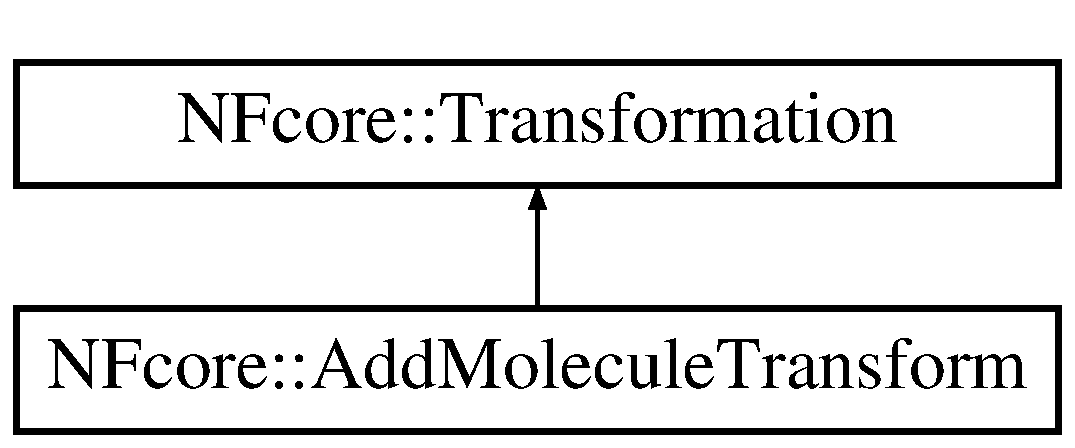
\includegraphics[height=2cm]{classNFcore_1_1AddMoleculeTransform}
\end{center}
\end{figure}
\subsection*{Public Member Functions}
\begin{CompactItemize}
\item 
{\bf AddMoleculeTransform} ({\bf SpeciesCreator} $\ast${\bf sc})
\item 
virtual {\bf $\sim$AddMoleculeTransform} ()
\item 
virtual void {\bf apply} ({\bf Mapping} $\ast$m, {\bf MappingSet} $\ast$$\ast$ms)
\item 
virtual int {\bf getComponentIndex} () const 
\end{CompactItemize}
\subsection*{Protected Attributes}
\begin{CompactItemize}
\item 
{\bf SpeciesCreator} $\ast$ {\bf sc}
\end{CompactItemize}


\subsection{Constructor \& Destructor Documentation}
\index{NFcore::AddMoleculeTransform@{NFcore::AddMoleculeTransform}!AddMoleculeTransform@{AddMoleculeTransform}}
\index{AddMoleculeTransform@{AddMoleculeTransform}!NFcore::AddMoleculeTransform@{NFcore::AddMoleculeTransform}}
\subsubsection{\setlength{\rightskip}{0pt plus 5cm}AddMoleculeTransform::AddMoleculeTransform ({\bf SpeciesCreator} $\ast$ {\em sc})}\label{classNFcore_1_1AddMoleculeTransform_93613b59c64a8f0147cab031647be7b7}


\index{NFcore::AddMoleculeTransform@{NFcore::AddMoleculeTransform}!$\sim$AddMoleculeTransform@{$\sim$AddMoleculeTransform}}
\index{$\sim$AddMoleculeTransform@{$\sim$AddMoleculeTransform}!NFcore::AddMoleculeTransform@{NFcore::AddMoleculeTransform}}
\subsubsection{\setlength{\rightskip}{0pt plus 5cm}AddMoleculeTransform::$\sim$AddMoleculeTransform ()\hspace{0.3cm}{\tt  [virtual]}}\label{classNFcore_1_1AddMoleculeTransform_2672f3a25595bacb7f64dfb3ddba8aa8}




\subsection{Member Function Documentation}
\index{NFcore::AddMoleculeTransform@{NFcore::AddMoleculeTransform}!apply@{apply}}
\index{apply@{apply}!NFcore::AddMoleculeTransform@{NFcore::AddMoleculeTransform}}
\subsubsection{\setlength{\rightskip}{0pt plus 5cm}void AddMoleculeTransform::apply ({\bf Mapping} $\ast$ {\em m}, {\bf MappingSet} $\ast$$\ast$ {\em ms})\hspace{0.3cm}{\tt  [virtual]}}\label{classNFcore_1_1AddMoleculeTransform_18b5845ce1e6d9c249acc40ff7b49dfd}




Implements {\bf NFcore::Transformation} \doxyref{}{p.}{classNFcore_1_1Transformation_6a57f607676c92b2465427e57bc7fae5}.\index{NFcore::AddMoleculeTransform@{NFcore::AddMoleculeTransform}!getComponentIndex@{getComponentIndex}}
\index{getComponentIndex@{getComponentIndex}!NFcore::AddMoleculeTransform@{NFcore::AddMoleculeTransform}}
\subsubsection{\setlength{\rightskip}{0pt plus 5cm}virtual int NFcore::AddMoleculeTransform::getComponentIndex () const\hspace{0.3cm}{\tt  [inline, virtual]}}\label{classNFcore_1_1AddMoleculeTransform_8a352eb7aa54568e417701461d507b9e}




Implements {\bf NFcore::Transformation} \doxyref{}{p.}{classNFcore_1_1Transformation_2ba394b20768b21ba328431103474607}.

\subsection{Member Data Documentation}
\index{NFcore::AddMoleculeTransform@{NFcore::AddMoleculeTransform}!sc@{sc}}
\index{sc@{sc}!NFcore::AddMoleculeTransform@{NFcore::AddMoleculeTransform}}
\subsubsection{\setlength{\rightskip}{0pt plus 5cm}{\bf SpeciesCreator}$\ast$ {\bf NFcore::AddMoleculeTransform::sc}\hspace{0.3cm}{\tt  [protected]}}\label{classNFcore_1_1AddMoleculeTransform_f36cd25da702f62343aed9a172f05af0}




The documentation for this class was generated from the following files:\begin{CompactItemize}
\item 
/home/msneddon/eclipse/galileoSR1\_\-cpp/workspace/NFsim/src/NFreactions/transformations/{\bf transformation.hh}\item 
/home/msneddon/eclipse/galileoSR1\_\-cpp/workspace/NFsim/src/NFreactions/transformations/{\bf transformation.cpp}\end{CompactItemize}

\section{NFcore::BasicRxnClass Class Reference}
\label{classNFcore_1_1BasicRxnClass}\index{NFcore::BasicRxnClass@{NFcore::BasicRxnClass}}
{\tt \#include $<$reaction.hh$>$}

Inheritance diagram for NFcore::BasicRxnClass::\begin{figure}[H]
\begin{center}
\leavevmode
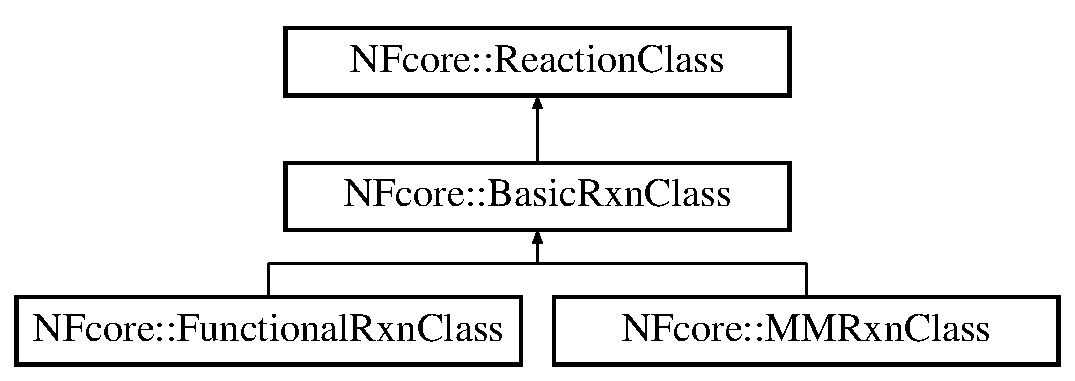
\includegraphics[height=3cm]{classNFcore_1_1BasicRxnClass}
\end{center}
\end{figure}
\subsection*{Public Member Functions}
\begin{CompactItemize}
\item 
{\bf BasicRxnClass} (string {\bf name}, double {\bf baseRate}, string baseRateName, {\bf TransformationSet} $\ast${\bf transformationSet}, {\bf System} $\ast$s)
\item 
virtual {\bf $\sim$BasicRxnClass} ()
\item 
virtual void {\bf init} ()
\item 
virtual void {\bf prepareForSimulation} ()
\item 
virtual bool {\bf tryToAdd} ({\bf Molecule} $\ast$m, unsigned int reactantPos)
\item 
virtual void {\bf remove} ({\bf Molecule} $\ast$m, unsigned int reactantPos)
\item 
virtual double {\bf update\_\-a} ()
\item 
virtual void {\bf notifyRateFactorChange} ({\bf Molecule} $\ast$m, int reactantIndex, int rxnListIndex)
\item 
virtual unsigned int {\bf getReactantCount} (unsigned int reactantIndex) const 
\item 
virtual void {\bf printFullDetails} () const 
\end{CompactItemize}
\subsection*{Protected Member Functions}
\begin{CompactItemize}
\item 
virtual void {\bf pickMappingSets} (double randNumber) const 
\end{CompactItemize}
\subsection*{Protected Attributes}
\begin{CompactItemize}
\item 
{\bf ReactantList} $\ast$$\ast$ {\bf reactantLists}
\item 
{\bf ReactantList} $\ast$ {\bf rl}
\item 
{\bf MappingSet} $\ast$ {\bf ms}
\end{CompactItemize}


\subsection{Constructor \& Destructor Documentation}
\index{NFcore::BasicRxnClass@{NFcore::BasicRxnClass}!BasicRxnClass@{BasicRxnClass}}
\index{BasicRxnClass@{BasicRxnClass}!NFcore::BasicRxnClass@{NFcore::BasicRxnClass}}
\subsubsection{\setlength{\rightskip}{0pt plus 5cm}BasicRxnClass::BasicRxnClass (string {\em name}, double {\em baseRate}, string {\em baseRateName}, {\bf TransformationSet} $\ast$ {\em transformationSet}, {\bf System} $\ast$ {\em s})}\label{classNFcore_1_1BasicRxnClass_d79da130b050650f7cdb63f1917d140f}


\index{NFcore::BasicRxnClass@{NFcore::BasicRxnClass}!$\sim$BasicRxnClass@{$\sim$BasicRxnClass}}
\index{$\sim$BasicRxnClass@{$\sim$BasicRxnClass}!NFcore::BasicRxnClass@{NFcore::BasicRxnClass}}
\subsubsection{\setlength{\rightskip}{0pt plus 5cm}BasicRxnClass::$\sim$BasicRxnClass ()\hspace{0.3cm}{\tt  [virtual]}}\label{classNFcore_1_1BasicRxnClass_67ba4f132c6376f31f3cddd1ff53abec}




\subsection{Member Function Documentation}
\index{NFcore::BasicRxnClass@{NFcore::BasicRxnClass}!init@{init}}
\index{init@{init}!NFcore::BasicRxnClass@{NFcore::BasicRxnClass}}
\subsubsection{\setlength{\rightskip}{0pt plus 5cm}void BasicRxnClass::init ()\hspace{0.3cm}{\tt  [virtual]}}\label{classNFcore_1_1BasicRxnClass_61147eb37d1d45be12a9e77cacd6bb92}




Implements {\bf NFcore::ReactionClass} \doxyref{}{p.}{classNFcore_1_1ReactionClass_fa3006801b4fcf821358bfca9bab8aa1}.\index{NFcore::BasicRxnClass@{NFcore::BasicRxnClass}!prepareForSimulation@{prepareForSimulation}}
\index{prepareForSimulation@{prepareForSimulation}!NFcore::BasicRxnClass@{NFcore::BasicRxnClass}}
\subsubsection{\setlength{\rightskip}{0pt plus 5cm}void BasicRxnClass::prepareForSimulation ()\hspace{0.3cm}{\tt  [virtual]}}\label{classNFcore_1_1BasicRxnClass_b96fd7ecb28984d28f0250bb4fc09631}




Implements {\bf NFcore::ReactionClass} \doxyref{}{p.}{classNFcore_1_1ReactionClass_f6466927590b894478fbe765f4da8aad}.\index{NFcore::BasicRxnClass@{NFcore::BasicRxnClass}!tryToAdd@{tryToAdd}}
\index{tryToAdd@{tryToAdd}!NFcore::BasicRxnClass@{NFcore::BasicRxnClass}}
\subsubsection{\setlength{\rightskip}{0pt plus 5cm}bool BasicRxnClass::tryToAdd ({\bf Molecule} $\ast$ {\em m}, unsigned int {\em reactantPos})\hspace{0.3cm}{\tt  [virtual]}}\label{classNFcore_1_1BasicRxnClass_56e941f00e4f503afb9519a6f23d30fd}




Implements {\bf NFcore::ReactionClass} \doxyref{}{p.}{classNFcore_1_1ReactionClass_7ef57431ab858d1039e9efedd011f1f0}.\index{NFcore::BasicRxnClass@{NFcore::BasicRxnClass}!remove@{remove}}
\index{remove@{remove}!NFcore::BasicRxnClass@{NFcore::BasicRxnClass}}
\subsubsection{\setlength{\rightskip}{0pt plus 5cm}void BasicRxnClass::remove ({\bf Molecule} $\ast$ {\em m}, unsigned int {\em reactantPos})\hspace{0.3cm}{\tt  [virtual]}}\label{classNFcore_1_1BasicRxnClass_4c3f8b5ff51c05a930aeeef6367ced23}




Implements {\bf NFcore::ReactionClass} \doxyref{}{p.}{classNFcore_1_1ReactionClass_e9f356905524d6e370059b1e4ef5754a}.\index{NFcore::BasicRxnClass@{NFcore::BasicRxnClass}!update\_\-a@{update\_\-a}}
\index{update\_\-a@{update\_\-a}!NFcore::BasicRxnClass@{NFcore::BasicRxnClass}}
\subsubsection{\setlength{\rightskip}{0pt plus 5cm}virtual double NFcore::BasicRxnClass::update\_\-a ()\hspace{0.3cm}{\tt  [inline, virtual]}}\label{classNFcore_1_1BasicRxnClass_9a679d57f4cfdd184f3bf312ecd20cc6}




Implements {\bf NFcore::ReactionClass} \doxyref{}{p.}{classNFcore_1_1ReactionClass_f5aed18705e78d14bd1a8f82068add70}.

Reimplemented in {\bf NFcore::PopulationRxnClass} \doxyref{}{p.}{classNFcore_1_1PopulationRxnClass_12585ef6755324a068e75ca7cc2cd7e9}, {\bf NFcore::FunctionalRxnClass} \doxyref{}{p.}{classNFcore_1_1FunctionalRxnClass_23dd5630ec0157ce7ab6d240720a57cb}, and {\bf NFcore::MMRxnClass} \doxyref{}{p.}{classNFcore_1_1MMRxnClass_63709cdada0fc7c63125bd2e562f4b42}.\index{NFcore::BasicRxnClass@{NFcore::BasicRxnClass}!notifyRateFactorChange@{notifyRateFactorChange}}
\index{notifyRateFactorChange@{notifyRateFactorChange}!NFcore::BasicRxnClass@{NFcore::BasicRxnClass}}
\subsubsection{\setlength{\rightskip}{0pt plus 5cm}void BasicRxnClass::notifyRateFactorChange ({\bf Molecule} $\ast$ {\em m}, int {\em reactantIndex}, int {\em rxnListIndex})\hspace{0.3cm}{\tt  [virtual]}}\label{classNFcore_1_1BasicRxnClass_ccc697e4b64efe0d4ced497cc886ece2}




Implements {\bf NFcore::ReactionClass} \doxyref{}{p.}{classNFcore_1_1ReactionClass_c18b82dc36c68699c00802201d7745cd}.\index{NFcore::BasicRxnClass@{NFcore::BasicRxnClass}!getReactantCount@{getReactantCount}}
\index{getReactantCount@{getReactantCount}!NFcore::BasicRxnClass@{NFcore::BasicRxnClass}}
\subsubsection{\setlength{\rightskip}{0pt plus 5cm}unsigned int BasicRxnClass::getReactantCount (unsigned int {\em reactantIndex}) const\hspace{0.3cm}{\tt  [virtual]}}\label{classNFcore_1_1BasicRxnClass_908c2d7fdceeb2c77f43d47275b707ff}




Implements {\bf NFcore::ReactionClass} \doxyref{}{p.}{classNFcore_1_1ReactionClass_a39fd321f4d58d79fa72812d65f1c762}.

Reimplemented in {\bf NFcore::PopulationRxnClass} \doxyref{}{p.}{classNFcore_1_1PopulationRxnClass_14c489c34e521228f5580a30e1018ffe}.\index{NFcore::BasicRxnClass@{NFcore::BasicRxnClass}!printFullDetails@{printFullDetails}}
\index{printFullDetails@{printFullDetails}!NFcore::BasicRxnClass@{NFcore::BasicRxnClass}}
\subsubsection{\setlength{\rightskip}{0pt plus 5cm}void BasicRxnClass::printFullDetails () const\hspace{0.3cm}{\tt  [virtual]}}\label{classNFcore_1_1BasicRxnClass_552dfb3cbcd194fef08e7c4ba773054e}




Implements {\bf NFcore::ReactionClass} \doxyref{}{p.}{classNFcore_1_1ReactionClass_521a0b7a474568522bec973cfa6b5242}.\index{NFcore::BasicRxnClass@{NFcore::BasicRxnClass}!pickMappingSets@{pickMappingSets}}
\index{pickMappingSets@{pickMappingSets}!NFcore::BasicRxnClass@{NFcore::BasicRxnClass}}
\subsubsection{\setlength{\rightskip}{0pt plus 5cm}void BasicRxnClass::pickMappingSets (double {\em randNumber}) const\hspace{0.3cm}{\tt  [protected, virtual]}}\label{classNFcore_1_1BasicRxnClass_8d194b51f6338bc68bc8440d02249f0e}




Implements {\bf NFcore::ReactionClass} \doxyref{}{p.}{classNFcore_1_1ReactionClass_ff3336a876f9e81904ee2b7be86bbdc5}.

Reimplemented in {\bf NFcore::PopulationRxnClass} \doxyref{}{p.}{classNFcore_1_1PopulationRxnClass_0004eb8b2a18ed687c975b7ba7e0b522}.

\subsection{Member Data Documentation}
\index{NFcore::BasicRxnClass@{NFcore::BasicRxnClass}!reactantLists@{reactantLists}}
\index{reactantLists@{reactantLists}!NFcore::BasicRxnClass@{NFcore::BasicRxnClass}}
\subsubsection{\setlength{\rightskip}{0pt plus 5cm}{\bf ReactantList}$\ast$$\ast$ {\bf NFcore::BasicRxnClass::reactantLists}\hspace{0.3cm}{\tt  [protected]}}\label{classNFcore_1_1BasicRxnClass_703547574659171f8048dfabe92fa022}


\index{NFcore::BasicRxnClass@{NFcore::BasicRxnClass}!rl@{rl}}
\index{rl@{rl}!NFcore::BasicRxnClass@{NFcore::BasicRxnClass}}
\subsubsection{\setlength{\rightskip}{0pt plus 5cm}{\bf ReactantList}$\ast$ {\bf NFcore::BasicRxnClass::rl}\hspace{0.3cm}{\tt  [protected]}}\label{classNFcore_1_1BasicRxnClass_fe4c53436947fbfeafeb01773f22d993}


\index{NFcore::BasicRxnClass@{NFcore::BasicRxnClass}!ms@{ms}}
\index{ms@{ms}!NFcore::BasicRxnClass@{NFcore::BasicRxnClass}}
\subsubsection{\setlength{\rightskip}{0pt plus 5cm}{\bf MappingSet}$\ast$ {\bf NFcore::BasicRxnClass::ms}\hspace{0.3cm}{\tt  [protected]}}\label{classNFcore_1_1BasicRxnClass_a3bece6f2cf817f3de725427708de47c}




The documentation for this class was generated from the following files:\begin{CompactItemize}
\item 
/home/msneddon/eclipse/indigo/workspace/NFsim/src/NFreactions/reactions/{\bf reaction.hh}\item 
/home/msneddon/eclipse/indigo/workspace/NFsim/src/NFreactions/reactions/{\bf reaction.cpp}\end{CompactItemize}

\section{NFcore::BindingSeparateComplexTransform Class Reference}
\label{classNFcore_1_1BindingSeparateComplexTransform}\index{NFcore::BindingSeparateComplexTransform@{NFcore::BindingSeparateComplexTransform}}
{\tt \#include $<$transformation.hh$>$}

Inheritance diagram for NFcore::BindingSeparateComplexTransform::\begin{figure}[H]
\begin{center}
\leavevmode
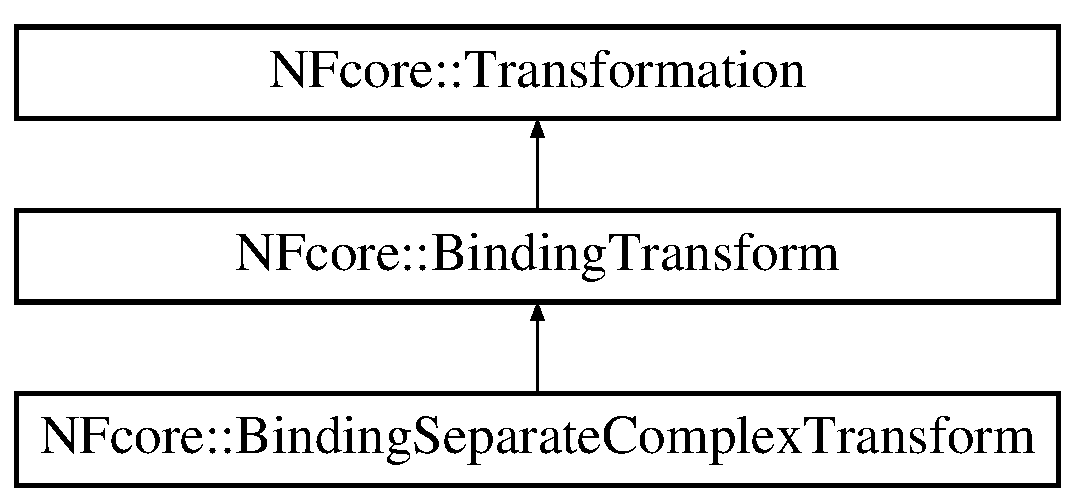
\includegraphics[height=3cm]{classNFcore_1_1BindingSeparateComplexTransform}
\end{center}
\end{figure}
\subsection*{Public Member Functions}
\begin{CompactItemize}
\item 
{\bf BindingSeparateComplexTransform} (int {\bf cIndex}, int {\bf otherReactantIndex}, int {\bf otherMappingIndex})
\item 
virtual {\bf $\sim$BindingSeparateComplexTransform} ()
\item 
virtual void {\bf apply} ({\bf Mapping} $\ast$m, {\bf MappingSet} $\ast$$\ast$ms)
\item 
virtual int {\bf getComponentIndex} () const 
\end{CompactItemize}


\subsection{Constructor \& Destructor Documentation}
\index{NFcore::BindingSeparateComplexTransform@{NFcore::BindingSeparateComplexTransform}!BindingSeparateComplexTransform@{BindingSeparateComplexTransform}}
\index{BindingSeparateComplexTransform@{BindingSeparateComplexTransform}!NFcore::BindingSeparateComplexTransform@{NFcore::BindingSeparateComplexTransform}}
\subsubsection{\setlength{\rightskip}{0pt plus 5cm}NFcore::BindingSeparateComplexTransform::BindingSeparateComplexTransform (int {\em cIndex}, int {\em otherReactantIndex}, int {\em otherMappingIndex})\hspace{0.3cm}{\tt  [inline]}}\label{classNFcore_1_1BindingSeparateComplexTransform_6b2b3334865d4cd91b782aef949a576d}


\index{NFcore::BindingSeparateComplexTransform@{NFcore::BindingSeparateComplexTransform}!$\sim$BindingSeparateComplexTransform@{$\sim$BindingSeparateComplexTransform}}
\index{$\sim$BindingSeparateComplexTransform@{$\sim$BindingSeparateComplexTransform}!NFcore::BindingSeparateComplexTransform@{NFcore::BindingSeparateComplexTransform}}
\subsubsection{\setlength{\rightskip}{0pt plus 5cm}virtual NFcore::BindingSeparateComplexTransform::$\sim$BindingSeparateComplexTransform ()\hspace{0.3cm}{\tt  [inline, virtual]}}\label{classNFcore_1_1BindingSeparateComplexTransform_dd3f3cf771abdedd39b0bd527acb2ec9}




\subsection{Member Function Documentation}
\index{NFcore::BindingSeparateComplexTransform@{NFcore::BindingSeparateComplexTransform}!apply@{apply}}
\index{apply@{apply}!NFcore::BindingSeparateComplexTransform@{NFcore::BindingSeparateComplexTransform}}
\subsubsection{\setlength{\rightskip}{0pt plus 5cm}void BindingSeparateComplexTransform::apply ({\bf Mapping} $\ast$ {\em m}, {\bf MappingSet} $\ast$$\ast$ {\em ms})\hspace{0.3cm}{\tt  [virtual]}}\label{classNFcore_1_1BindingSeparateComplexTransform_af8be6214ca8a9a4041754bb3189ca09}




Reimplemented from {\bf NFcore::BindingTransform} \doxyref{}{p.}{classNFcore_1_1BindingTransform_45f7022ec7b76e0ba90021de650026e9}.\index{NFcore::BindingSeparateComplexTransform@{NFcore::BindingSeparateComplexTransform}!getComponentIndex@{getComponentIndex}}
\index{getComponentIndex@{getComponentIndex}!NFcore::BindingSeparateComplexTransform@{NFcore::BindingSeparateComplexTransform}}
\subsubsection{\setlength{\rightskip}{0pt plus 5cm}virtual int NFcore::BindingSeparateComplexTransform::getComponentIndex () const\hspace{0.3cm}{\tt  [inline, virtual]}}\label{classNFcore_1_1BindingSeparateComplexTransform_5ea6920bf3d0a5fb624cff52cf0c97ce}




Reimplemented from {\bf NFcore::BindingTransform} \doxyref{}{p.}{classNFcore_1_1BindingTransform_9dad3bcc59c0c0dfd316fc494b7689be}.

The documentation for this class was generated from the following files:\begin{CompactItemize}
\item 
/home/msneddon/eclipse/indigo/workspace/NFsim/src/NFreactions/transformations/{\bf transformation.hh}\item 
/home/msneddon/eclipse/indigo/workspace/NFsim/src/NFreactions/transformations/{\bf transformation.cpp}\end{CompactItemize}

\section{NFcore::BindingTransform Class Reference}
\label{classNFcore_1_1BindingTransform}\index{NFcore::BindingTransform@{NFcore::BindingTransform}}
{\tt \#include $<$transformation.hh$>$}

Inheritance diagram for NFcore::BindingTransform::\begin{figure}[H]
\begin{center}
\leavevmode
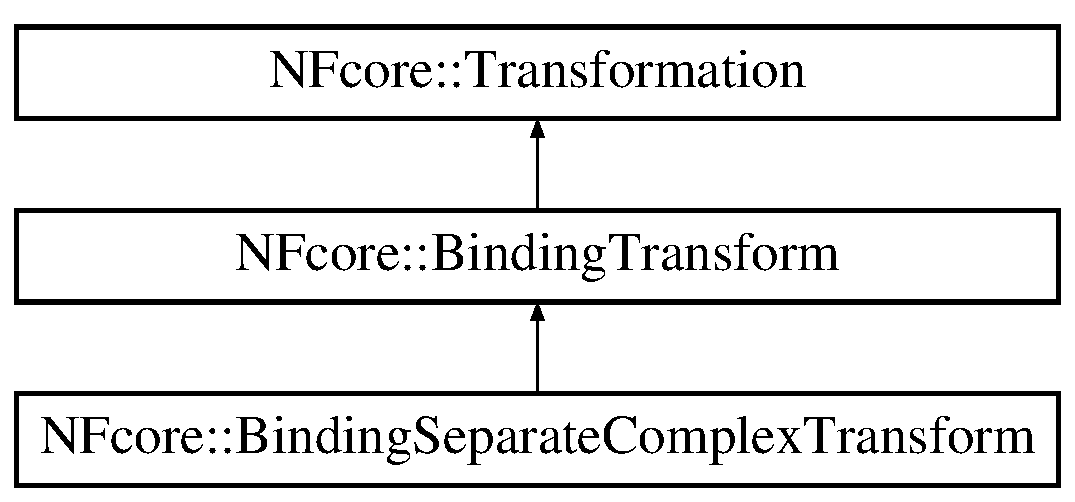
\includegraphics[height=3cm]{classNFcore_1_1BindingTransform}
\end{center}
\end{figure}
\subsection*{Public Member Functions}
\begin{CompactItemize}
\item 
{\bf BindingTransform} (int {\bf cIndex}, int {\bf otherReactantIndex}, int {\bf otherMappingIndex})
\item 
virtual {\bf $\sim$BindingTransform} ()
\item 
virtual void {\bf apply} ({\bf Mapping} $\ast$m, {\bf MappingSet} $\ast$$\ast$ms)
\item 
virtual int {\bf getComponentIndex} () const 
\item 
virtual bool {\bf checkForNullCondition} ({\bf Mapping} $\ast$m, {\bf MappingSet} $\ast$$\ast$ms)
\end{CompactItemize}
\subsection*{Protected Attributes}
\begin{CompactItemize}
\item 
int {\bf cIndex}
\item 
int {\bf otherReactantIndex}
\item 
int {\bf otherMappingIndex}
\end{CompactItemize}


\subsection{Constructor \& Destructor Documentation}
\index{NFcore::BindingTransform@{NFcore::BindingTransform}!BindingTransform@{BindingTransform}}
\index{BindingTransform@{BindingTransform}!NFcore::BindingTransform@{NFcore::BindingTransform}}
\subsubsection{\setlength{\rightskip}{0pt plus 5cm}BindingTransform::BindingTransform (int {\em cIndex}, int {\em otherReactantIndex}, int {\em otherMappingIndex})}\label{classNFcore_1_1BindingTransform_9083530eac9c733f197d2e4d7c25dc4f}


\index{NFcore::BindingTransform@{NFcore::BindingTransform}!$\sim$BindingTransform@{$\sim$BindingTransform}}
\index{$\sim$BindingTransform@{$\sim$BindingTransform}!NFcore::BindingTransform@{NFcore::BindingTransform}}
\subsubsection{\setlength{\rightskip}{0pt plus 5cm}virtual NFcore::BindingTransform::$\sim$BindingTransform ()\hspace{0.3cm}{\tt  [inline, virtual]}}\label{classNFcore_1_1BindingTransform_10dedfd9cfc4c6e0d383833dfa98f485}




\subsection{Member Function Documentation}
\index{NFcore::BindingTransform@{NFcore::BindingTransform}!apply@{apply}}
\index{apply@{apply}!NFcore::BindingTransform@{NFcore::BindingTransform}}
\subsubsection{\setlength{\rightskip}{0pt plus 5cm}void BindingTransform::apply ({\bf Mapping} $\ast$ {\em m}, {\bf MappingSet} $\ast$$\ast$ {\em ms})\hspace{0.3cm}{\tt  [virtual]}}\label{classNFcore_1_1BindingTransform_45f7022ec7b76e0ba90021de650026e9}




Implements {\bf NFcore::Transformation} \doxyref{}{p.}{classNFcore_1_1Transformation_6a57f607676c92b2465427e57bc7fae5}.\index{NFcore::BindingTransform@{NFcore::BindingTransform}!getComponentIndex@{getComponentIndex}}
\index{getComponentIndex@{getComponentIndex}!NFcore::BindingTransform@{NFcore::BindingTransform}}
\subsubsection{\setlength{\rightskip}{0pt plus 5cm}virtual int NFcore::BindingTransform::getComponentIndex () const\hspace{0.3cm}{\tt  [inline, virtual]}}\label{classNFcore_1_1BindingTransform_9dad3bcc59c0c0dfd316fc494b7689be}




Implements {\bf NFcore::Transformation} \doxyref{}{p.}{classNFcore_1_1Transformation_2ba394b20768b21ba328431103474607}.\index{NFcore::BindingTransform@{NFcore::BindingTransform}!checkForNullCondition@{checkForNullCondition}}
\index{checkForNullCondition@{checkForNullCondition}!NFcore::BindingTransform@{NFcore::BindingTransform}}
\subsubsection{\setlength{\rightskip}{0pt plus 5cm}bool BindingTransform::checkForNullCondition ({\bf Mapping} $\ast$ {\em m}, {\bf MappingSet} $\ast$$\ast$ {\em ms})\hspace{0.3cm}{\tt  [virtual]}}\label{classNFcore_1_1BindingTransform_0bec86cfe6a25c759030797865e317a5}




Reimplemented from {\bf NFcore::Transformation} \doxyref{}{p.}{classNFcore_1_1Transformation_1f9aef7f2a2435e3116224884afccc83}.

Reimplemented in {\bf NFcore::NewMoleculeBindingTransform} \doxyref{}{p.}{classNFcore_1_1NewMoleculeBindingTransform_422103cefcdcef333619990c20a8b16a}.

\subsection{Member Data Documentation}
\index{NFcore::BindingTransform@{NFcore::BindingTransform}!cIndex@{cIndex}}
\index{cIndex@{cIndex}!NFcore::BindingTransform@{NFcore::BindingTransform}}
\subsubsection{\setlength{\rightskip}{0pt plus 5cm}int {\bf NFcore::BindingTransform::cIndex}\hspace{0.3cm}{\tt  [protected]}}\label{classNFcore_1_1BindingTransform_69746a4bc7d57793bfa42ea8a9494062}


\index{NFcore::BindingTransform@{NFcore::BindingTransform}!otherReactantIndex@{otherReactantIndex}}
\index{otherReactantIndex@{otherReactantIndex}!NFcore::BindingTransform@{NFcore::BindingTransform}}
\subsubsection{\setlength{\rightskip}{0pt plus 5cm}int {\bf NFcore::BindingTransform::otherReactantIndex}\hspace{0.3cm}{\tt  [protected]}}\label{classNFcore_1_1BindingTransform_633ed124b8379e9a79acc3c17fe2def7}


\index{NFcore::BindingTransform@{NFcore::BindingTransform}!otherMappingIndex@{otherMappingIndex}}
\index{otherMappingIndex@{otherMappingIndex}!NFcore::BindingTransform@{NFcore::BindingTransform}}
\subsubsection{\setlength{\rightskip}{0pt plus 5cm}int {\bf NFcore::BindingTransform::otherMappingIndex}\hspace{0.3cm}{\tt  [protected]}}\label{classNFcore_1_1BindingTransform_2abab37cc82da3f331dd68183d77f44b}




The documentation for this class was generated from the following files:\begin{CompactItemize}
\item 
/home/msneddon/eclipse/indigo/workspace/NFsim/src/NFreactions/transformations/{\bf transformation.hh}\item 
/home/msneddon/eclipse/indigo/workspace/NFsim/src/NFreactions/transformations/{\bf transformation.cpp}\end{CompactItemize}

\section{NFcore::Complex Class Reference}
\label{classNFcore_1_1Complex}\index{NFcore::Complex@{NFcore::Complex}}
{\tt \#include $<$NFcore.hh$>$}



\subsection{Detailed Description}
Container to dynamically keep track of all system complexes. 

\begin{Desc}
\item[Author:]Michael Sneddon \end{Desc}
\subsection*{Public Member Functions}
\begin{CompactItemize}
\item 
{\bf Complex} ({\bf System} $\ast$s, int {\bf ID\_\-complex}, {\bf Molecule} $\ast$m)
\item 
{\bf $\sim$Complex} ()
\item 
bool {\bf isAlive} ()
\item 
int {\bf getComplexID} () const 
\item 
int {\bf getComplexSize} () const 
\item 
int {\bf getMoleculeCountOfType} ({\bf MoleculeType} $\ast$m)
\item 
void {\bf mergeWithList} ({\bf Complex} $\ast$c)
\item 
void {\bf updateComplexMembership} ({\bf Molecule} $\ast$m)
\item 
void {\bf refactorToNewComplex} (int new\_\-ID\_\-complex)
\item 
void {\bf emptyComplexForever} ()
\item 
void {\bf printDegreeDistribution} ()
\item 
void {\bf getDegreeDistribution} (vector$<$ int $>$ \&degreeDist)
\item 
void {\bf printDetails} ()
\item 
void {\bf printDetailsLong} ()
\item 
double {\bf getDistance} ({\bf Complex} $\ast$c)
\item 
double {\bf getXpos} ()
\item 
double {\bf getYpos} ()
\item 
double {\bf getZpos} ()
\end{CompactItemize}
\subsection*{Public Attributes}
\begin{CompactItemize}
\item 
list$<$ {\bf Molecule} $\ast$ $>$ {\bf complexMembers}
\item 
list$<$ {\bf Molecule} $\ast$ $>$::iterator {\bf molIter}
\end{CompactItemize}
\subsection*{Static Public Attributes}
\begin{CompactItemize}
\item 
static const int {\bf UNIFORM} = 0
\item 
static const int {\bf FIXED\_\-POINT} = 1
\item 
static const int {\bf DIFFUSE\_\-3D} = 2
\end{CompactItemize}
\subsection*{Protected Attributes}
\begin{CompactItemize}
\item 
{\bf System} $\ast$ {\bf system}
\item 
int {\bf ID\_\-complex}
\end{CompactItemize}


\subsection{Constructor \& Destructor Documentation}
\index{NFcore::Complex@{NFcore::Complex}!Complex@{Complex}}
\index{Complex@{Complex}!NFcore::Complex@{NFcore::Complex}}
\subsubsection{\setlength{\rightskip}{0pt plus 5cm}Complex::Complex ({\bf System} $\ast$ {\em s}, int {\em ID\_\-complex}, {\bf Molecule} $\ast$ {\em m})}\label{classNFcore_1_1Complex_f21fb570112128eaf141081404504a67}


\index{NFcore::Complex@{NFcore::Complex}!$\sim$Complex@{$\sim$Complex}}
\index{$\sim$Complex@{$\sim$Complex}!NFcore::Complex@{NFcore::Complex}}
\subsubsection{\setlength{\rightskip}{0pt plus 5cm}Complex::$\sim$Complex ()}\label{classNFcore_1_1Complex_70e14b17c92e3da779686b98f9f3bb2d}




\subsection{Member Function Documentation}
\index{NFcore::Complex@{NFcore::Complex}!isAlive@{isAlive}}
\index{isAlive@{isAlive}!NFcore::Complex@{NFcore::Complex}}
\subsubsection{\setlength{\rightskip}{0pt plus 5cm}bool Complex::isAlive ()}\label{classNFcore_1_1Complex_2b4bfa37f0d9767e387a18ba9764d181}


\index{NFcore::Complex@{NFcore::Complex}!getComplexID@{getComplexID}}
\index{getComplexID@{getComplexID}!NFcore::Complex@{NFcore::Complex}}
\subsubsection{\setlength{\rightskip}{0pt plus 5cm}int NFcore::Complex::getComplexID () const\hspace{0.3cm}{\tt  [inline]}}\label{classNFcore_1_1Complex_72339ce32267d5aab1dfaa573a281d5c}


\index{NFcore::Complex@{NFcore::Complex}!getComplexSize@{getComplexSize}}
\index{getComplexSize@{getComplexSize}!NFcore::Complex@{NFcore::Complex}}
\subsubsection{\setlength{\rightskip}{0pt plus 5cm}int NFcore::Complex::getComplexSize () const\hspace{0.3cm}{\tt  [inline]}}\label{classNFcore_1_1Complex_8ee0c095d1fddd3e0e758ff0cdb29b27}


\index{NFcore::Complex@{NFcore::Complex}!getMoleculeCountOfType@{getMoleculeCountOfType}}
\index{getMoleculeCountOfType@{getMoleculeCountOfType}!NFcore::Complex@{NFcore::Complex}}
\subsubsection{\setlength{\rightskip}{0pt plus 5cm}int Complex::getMoleculeCountOfType ({\bf MoleculeType} $\ast$ {\em m})}\label{classNFcore_1_1Complex_7ef1c1b74f0d87d95e7ffa10f2120a4a}


\index{NFcore::Complex@{NFcore::Complex}!mergeWithList@{mergeWithList}}
\index{mergeWithList@{mergeWithList}!NFcore::Complex@{NFcore::Complex}}
\subsubsection{\setlength{\rightskip}{0pt plus 5cm}void Complex::mergeWithList ({\bf Complex} $\ast$ {\em c})}\label{classNFcore_1_1Complex_a11aaab6753e3e2b0ce594a878721b1d}


\index{NFcore::Complex@{NFcore::Complex}!updateComplexMembership@{updateComplexMembership}}
\index{updateComplexMembership@{updateComplexMembership}!NFcore::Complex@{NFcore::Complex}}
\subsubsection{\setlength{\rightskip}{0pt plus 5cm}void Complex::updateComplexMembership ({\bf Molecule} $\ast$ {\em m})}\label{classNFcore_1_1Complex_dab8d5e7e2ac410d7469e6d8f17ac998}


\index{NFcore::Complex@{NFcore::Complex}!refactorToNewComplex@{refactorToNewComplex}}
\index{refactorToNewComplex@{refactorToNewComplex}!NFcore::Complex@{NFcore::Complex}}
\subsubsection{\setlength{\rightskip}{0pt plus 5cm}void Complex::refactorToNewComplex (int {\em new\_\-ID\_\-complex})}\label{classNFcore_1_1Complex_456f86fedae315aa417f12a0589dbac1}


\index{NFcore::Complex@{NFcore::Complex}!emptyComplexForever@{emptyComplexForever}}
\index{emptyComplexForever@{emptyComplexForever}!NFcore::Complex@{NFcore::Complex}}
\subsubsection{\setlength{\rightskip}{0pt plus 5cm}void NFcore::Complex::emptyComplexForever ()\hspace{0.3cm}{\tt  [inline]}}\label{classNFcore_1_1Complex_2e22d230882b9d1dfdea9ecf0c743440}


\index{NFcore::Complex@{NFcore::Complex}!printDegreeDistribution@{printDegreeDistribution}}
\index{printDegreeDistribution@{printDegreeDistribution}!NFcore::Complex@{NFcore::Complex}}
\subsubsection{\setlength{\rightskip}{0pt plus 5cm}void Complex::printDegreeDistribution ()}\label{classNFcore_1_1Complex_ade8e1f169483806a9e0d4fcc0092390}


\index{NFcore::Complex@{NFcore::Complex}!getDegreeDistribution@{getDegreeDistribution}}
\index{getDegreeDistribution@{getDegreeDistribution}!NFcore::Complex@{NFcore::Complex}}
\subsubsection{\setlength{\rightskip}{0pt plus 5cm}void Complex::getDegreeDistribution (vector$<$ int $>$ \& {\em degreeDist})}\label{classNFcore_1_1Complex_4d11db80f44edc51ccfc98d50a9a2125}


\index{NFcore::Complex@{NFcore::Complex}!printDetails@{printDetails}}
\index{printDetails@{printDetails}!NFcore::Complex@{NFcore::Complex}}
\subsubsection{\setlength{\rightskip}{0pt plus 5cm}void Complex::printDetails ()}\label{classNFcore_1_1Complex_c2b10523459c98c2d465a8fbe63f0536}


\index{NFcore::Complex@{NFcore::Complex}!printDetailsLong@{printDetailsLong}}
\index{printDetailsLong@{printDetailsLong}!NFcore::Complex@{NFcore::Complex}}
\subsubsection{\setlength{\rightskip}{0pt plus 5cm}void Complex::printDetailsLong ()}\label{classNFcore_1_1Complex_7eef40d39a4eabc6519cbaddd28e8071}


\index{NFcore::Complex@{NFcore::Complex}!getDistance@{getDistance}}
\index{getDistance@{getDistance}!NFcore::Complex@{NFcore::Complex}}
\subsubsection{\setlength{\rightskip}{0pt plus 5cm}double NFcore::Complex::getDistance ({\bf Complex} $\ast$ {\em c})\hspace{0.3cm}{\tt  [inline]}}\label{classNFcore_1_1Complex_5b68ccedb435018ecbecfc2d87efe13a}


\index{NFcore::Complex@{NFcore::Complex}!getXpos@{getXpos}}
\index{getXpos@{getXpos}!NFcore::Complex@{NFcore::Complex}}
\subsubsection{\setlength{\rightskip}{0pt plus 5cm}double NFcore::Complex::getXpos ()\hspace{0.3cm}{\tt  [inline]}}\label{classNFcore_1_1Complex_13118693140f69e620ec1c16daec9094}


\index{NFcore::Complex@{NFcore::Complex}!getYpos@{getYpos}}
\index{getYpos@{getYpos}!NFcore::Complex@{NFcore::Complex}}
\subsubsection{\setlength{\rightskip}{0pt plus 5cm}double NFcore::Complex::getYpos ()\hspace{0.3cm}{\tt  [inline]}}\label{classNFcore_1_1Complex_fd1731cf30137d822365c551233d9619}


\index{NFcore::Complex@{NFcore::Complex}!getZpos@{getZpos}}
\index{getZpos@{getZpos}!NFcore::Complex@{NFcore::Complex}}
\subsubsection{\setlength{\rightskip}{0pt plus 5cm}double NFcore::Complex::getZpos ()\hspace{0.3cm}{\tt  [inline]}}\label{classNFcore_1_1Complex_e1a2b42aaefbcccf6cbc72f1269f7321}




\subsection{Member Data Documentation}
\index{NFcore::Complex@{NFcore::Complex}!UNIFORM@{UNIFORM}}
\index{UNIFORM@{UNIFORM}!NFcore::Complex@{NFcore::Complex}}
\subsubsection{\setlength{\rightskip}{0pt plus 5cm}const int {\bf NFcore::Complex::UNIFORM} = 0\hspace{0.3cm}{\tt  [static]}}\label{classNFcore_1_1Complex_15091c1106920e003a2e9b060f158f39}


\index{NFcore::Complex@{NFcore::Complex}!FIXED\_\-POINT@{FIXED\_\-POINT}}
\index{FIXED\_\-POINT@{FIXED\_\-POINT}!NFcore::Complex@{NFcore::Complex}}
\subsubsection{\setlength{\rightskip}{0pt plus 5cm}const int {\bf NFcore::Complex::FIXED\_\-POINT} = 1\hspace{0.3cm}{\tt  [static]}}\label{classNFcore_1_1Complex_6a246e3f3d3523d409a6bc22ee955885}


\index{NFcore::Complex@{NFcore::Complex}!DIFFUSE\_\-3D@{DIFFUSE\_\-3D}}
\index{DIFFUSE\_\-3D@{DIFFUSE\_\-3D}!NFcore::Complex@{NFcore::Complex}}
\subsubsection{\setlength{\rightskip}{0pt plus 5cm}const int {\bf NFcore::Complex::DIFFUSE\_\-3D} = 2\hspace{0.3cm}{\tt  [static]}}\label{classNFcore_1_1Complex_f647fd600ba3d9d6fd5025ca68c17a50}


\index{NFcore::Complex@{NFcore::Complex}!complexMembers@{complexMembers}}
\index{complexMembers@{complexMembers}!NFcore::Complex@{NFcore::Complex}}
\subsubsection{\setlength{\rightskip}{0pt plus 5cm}list$<${\bf Molecule} $\ast$$>$ {\bf NFcore::Complex::complexMembers}}\label{classNFcore_1_1Complex_eb6d1fcb66f1c7ae39edb701f1443024}


\index{NFcore::Complex@{NFcore::Complex}!molIter@{molIter}}
\index{molIter@{molIter}!NFcore::Complex@{NFcore::Complex}}
\subsubsection{\setlength{\rightskip}{0pt plus 5cm}list$<${\bf Molecule} $\ast$$>$::iterator {\bf NFcore::Complex::molIter}}\label{classNFcore_1_1Complex_2551a54dfa379df3bc200b729e3e35bf}


\index{NFcore::Complex@{NFcore::Complex}!system@{system}}
\index{system@{system}!NFcore::Complex@{NFcore::Complex}}
\subsubsection{\setlength{\rightskip}{0pt plus 5cm}{\bf System}$\ast$ {\bf NFcore::Complex::system}\hspace{0.3cm}{\tt  [protected]}}\label{classNFcore_1_1Complex_507911a7d8e341fe531173a178011cc3}


\index{NFcore::Complex@{NFcore::Complex}!ID\_\-complex@{ID\_\-complex}}
\index{ID\_\-complex@{ID\_\-complex}!NFcore::Complex@{NFcore::Complex}}
\subsubsection{\setlength{\rightskip}{0pt plus 5cm}int {\bf NFcore::Complex::ID\_\-complex}\hspace{0.3cm}{\tt  [protected]}}\label{classNFcore_1_1Complex_fa83ffe4d89fe79396145cf245960d9d}




The documentation for this class was generated from the following files:\begin{CompactItemize}
\item 
/home/msneddon/eclipse/galileoSR1\_\-cpp/workspace/NFsim/src/NFcore/{\bf NFcore.hh}\item 
/home/msneddon/eclipse/galileoSR1\_\-cpp/workspace/NFsim/src/NFcore/{\bf complex.cpp}\end{CompactItemize}

\section{NFinput::component Class Reference}
\label{classNFinput_1_1component}\index{NFinput::component@{NFinput::component}}
{\tt \#include $<$NFinput.hh$>$}



\subsection{Detailed Description}
Maintains information about a \doxyref{component}{p.}{classNFinput_1_1component} of a TemplateMolecule. 

\begin{Desc}
\item[Author:]Michael Sneddon \end{Desc}
\subsection*{Public Member Functions}
\begin{CompactItemize}
\item 
{\bf component} ({\bf TemplateMolecule} $\ast${\bf t}, string {\bf name})
\item 
{\bf component} ({\bf MoleculeType} $\ast${\bf mt}, string {\bf name})
\item 
{\bf $\sim$component} ()
\end{CompactItemize}
\subsection*{Public Attributes}
\begin{CompactItemize}
\item 
{\bf TemplateMolecule} $\ast$ {\bf t}
\item 
{\bf MoleculeType} $\ast$ {\bf mt}
\item 
string {\bf name}
\item 
string {\bf uniqueId}
\item 
string {\bf symPermutationName}
\item 
string {\bf numOfBondsLabel}
\item 
string {\bf stateConstraintLabel}
\end{CompactItemize}


\subsection{Constructor \& Destructor Documentation}
\index{NFinput::component@{NFinput::component}!component@{component}}
\index{component@{component}!NFinput::component@{NFinput::component}}
\subsubsection{\setlength{\rightskip}{0pt plus 5cm}component::component ({\bf TemplateMolecule} $\ast$ {\em t}, string {\em name})}\label{classNFinput_1_1component_478cf998a7db82c3716290f41e2ede3c}


\index{NFinput::component@{NFinput::component}!component@{component}}
\index{component@{component}!NFinput::component@{NFinput::component}}
\subsubsection{\setlength{\rightskip}{0pt plus 5cm}component::component ({\bf MoleculeType} $\ast$ {\em mt}, string {\em name})}\label{classNFinput_1_1component_b5e7b80a96923dc24d38ba2c38878d43}


\index{NFinput::component@{NFinput::component}!$\sim$component@{$\sim$component}}
\index{$\sim$component@{$\sim$component}!NFinput::component@{NFinput::component}}
\subsubsection{\setlength{\rightskip}{0pt plus 5cm}component::$\sim$component ()}\label{classNFinput_1_1component_fff0b30c9d2d257b3dd0c572614d5bcb}




\subsection{Member Data Documentation}
\index{NFinput::component@{NFinput::component}!t@{t}}
\index{t@{t}!NFinput::component@{NFinput::component}}
\subsubsection{\setlength{\rightskip}{0pt plus 5cm}{\bf TemplateMolecule}$\ast$ {\bf NFinput::component::t}}\label{classNFinput_1_1component_82a0ca29c823a89050beea84bc620173}


\index{NFinput::component@{NFinput::component}!mt@{mt}}
\index{mt@{mt}!NFinput::component@{NFinput::component}}
\subsubsection{\setlength{\rightskip}{0pt plus 5cm}{\bf MoleculeType}$\ast$ {\bf NFinput::component::mt}}\label{classNFinput_1_1component_7946677cd6d9ac23b8bf2a691b4e3598}


\index{NFinput::component@{NFinput::component}!name@{name}}
\index{name@{name}!NFinput::component@{NFinput::component}}
\subsubsection{\setlength{\rightskip}{0pt plus 5cm}string {\bf NFinput::component::name}}\label{classNFinput_1_1component_65defb28bf783d69c27bac3106d9fa20}


\index{NFinput::component@{NFinput::component}!uniqueId@{uniqueId}}
\index{uniqueId@{uniqueId}!NFinput::component@{NFinput::component}}
\subsubsection{\setlength{\rightskip}{0pt plus 5cm}string {\bf NFinput::component::uniqueId}}\label{classNFinput_1_1component_38a260df183cd27e77c21dbbf2f80743}


\index{NFinput::component@{NFinput::component}!symPermutationName@{symPermutationName}}
\index{symPermutationName@{symPermutationName}!NFinput::component@{NFinput::component}}
\subsubsection{\setlength{\rightskip}{0pt plus 5cm}string {\bf NFinput::component::symPermutationName}}\label{classNFinput_1_1component_0644b483cc51364449774a44fe3d9f21}


\index{NFinput::component@{NFinput::component}!numOfBondsLabel@{numOfBondsLabel}}
\index{numOfBondsLabel@{numOfBondsLabel}!NFinput::component@{NFinput::component}}
\subsubsection{\setlength{\rightskip}{0pt plus 5cm}string {\bf NFinput::component::numOfBondsLabel}}\label{classNFinput_1_1component_5cf73e201edb854a151ee9b9c83b4b22}


\index{NFinput::component@{NFinput::component}!stateConstraintLabel@{stateConstraintLabel}}
\index{stateConstraintLabel@{stateConstraintLabel}!NFinput::component@{NFinput::component}}
\subsubsection{\setlength{\rightskip}{0pt plus 5cm}string {\bf NFinput::component::stateConstraintLabel}}\label{classNFinput_1_1component_bdde1cac2b7ebc8da3be50dfb093cffe}




The documentation for this class was generated from the following files:\begin{CompactItemize}
\item 
/home/msneddon/eclipse/indigo/workspace/NFsim/src/NFinput/{\bf NFinput.hh}\item 
/home/msneddon/eclipse/indigo/workspace/NFsim/src/NFinput/{\bf NFinput.cpp}\end{CompactItemize}

\section{NFcore::DecrementStateTransform Class Reference}
\label{classNFcore_1_1DecrementStateTransform}\index{NFcore::DecrementStateTransform@{NFcore::DecrementStateTransform}}
{\tt \#include $<$transformation.hh$>$}

Inheritance diagram for NFcore::DecrementStateTransform::\begin{figure}[H]
\begin{center}
\leavevmode
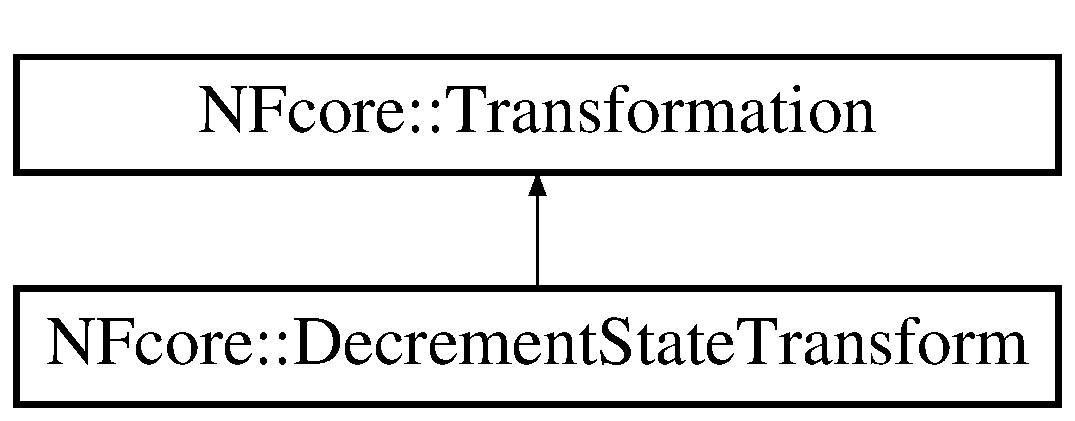
\includegraphics[height=2cm]{classNFcore_1_1DecrementStateTransform}
\end{center}
\end{figure}
\subsection*{Public Member Functions}
\begin{CompactItemize}
\item 
{\bf DecrementStateTransform} (unsigned int stateIndex)
\item 
virtual {\bf $\sim$DecrementStateTransform} ()
\item 
virtual void {\bf apply} ({\bf Mapping} $\ast$m, {\bf MappingSet} $\ast$$\ast$ms)
\item 
virtual int {\bf getComponentIndex} () const 
\end{CompactItemize}
\subsection*{Protected Attributes}
\begin{CompactItemize}
\item 
int {\bf cIndex}
\end{CompactItemize}


\subsection{Constructor \& Destructor Documentation}
\index{NFcore::DecrementStateTransform@{NFcore::DecrementStateTransform}!DecrementStateTransform@{DecrementStateTransform}}
\index{DecrementStateTransform@{DecrementStateTransform}!NFcore::DecrementStateTransform@{NFcore::DecrementStateTransform}}
\subsubsection{\setlength{\rightskip}{0pt plus 5cm}DecrementStateTransform::DecrementStateTransform (unsigned int {\em stateIndex})}\label{classNFcore_1_1DecrementStateTransform_807f5dcf8a4e36260f07de4bca59b9b1}


\index{NFcore::DecrementStateTransform@{NFcore::DecrementStateTransform}!$\sim$DecrementStateTransform@{$\sim$DecrementStateTransform}}
\index{$\sim$DecrementStateTransform@{$\sim$DecrementStateTransform}!NFcore::DecrementStateTransform@{NFcore::DecrementStateTransform}}
\subsubsection{\setlength{\rightskip}{0pt plus 5cm}virtual NFcore::DecrementStateTransform::$\sim$DecrementStateTransform ()\hspace{0.3cm}{\tt  [inline, virtual]}}\label{classNFcore_1_1DecrementStateTransform_0834e9d6ea154bd438ebbf459f8e2899}




\subsection{Member Function Documentation}
\index{NFcore::DecrementStateTransform@{NFcore::DecrementStateTransform}!apply@{apply}}
\index{apply@{apply}!NFcore::DecrementStateTransform@{NFcore::DecrementStateTransform}}
\subsubsection{\setlength{\rightskip}{0pt plus 5cm}void DecrementStateTransform::apply ({\bf Mapping} $\ast$ {\em m}, {\bf MappingSet} $\ast$$\ast$ {\em ms})\hspace{0.3cm}{\tt  [virtual]}}\label{classNFcore_1_1DecrementStateTransform_2094268f2958cc380cc9ec1c8a8332da}




Implements {\bf NFcore::Transformation} \doxyref{}{p.}{classNFcore_1_1Transformation_6a57f607676c92b2465427e57bc7fae5}.\index{NFcore::DecrementStateTransform@{NFcore::DecrementStateTransform}!getComponentIndex@{getComponentIndex}}
\index{getComponentIndex@{getComponentIndex}!NFcore::DecrementStateTransform@{NFcore::DecrementStateTransform}}
\subsubsection{\setlength{\rightskip}{0pt plus 5cm}virtual int NFcore::DecrementStateTransform::getComponentIndex () const\hspace{0.3cm}{\tt  [inline, virtual]}}\label{classNFcore_1_1DecrementStateTransform_8609049e75d2a31fb64c32f1608565bf}




Implements {\bf NFcore::Transformation} \doxyref{}{p.}{classNFcore_1_1Transformation_2ba394b20768b21ba328431103474607}.

\subsection{Member Data Documentation}
\index{NFcore::DecrementStateTransform@{NFcore::DecrementStateTransform}!cIndex@{cIndex}}
\index{cIndex@{cIndex}!NFcore::DecrementStateTransform@{NFcore::DecrementStateTransform}}
\subsubsection{\setlength{\rightskip}{0pt plus 5cm}int {\bf NFcore::DecrementStateTransform::cIndex}\hspace{0.3cm}{\tt  [protected]}}\label{classNFcore_1_1DecrementStateTransform_371fe6418e6908bd426111f62fa5f462}




The documentation for this class was generated from the following files:\begin{CompactItemize}
\item 
/home/msneddon/eclipse/ganymede\_\-cpp/workspace/NFsim\_\-svn/src/NFreactions/transformations/{\bf transformation.hh}\item 
/home/msneddon/eclipse/ganymede\_\-cpp/workspace/NFsim\_\-svn/src/NFreactions/transformations/{\bf transformation.cpp}\end{CompactItemize}

\section{NFcore::DORRxnClass Class Reference}
\label{classNFcore_1_1DORRxnClass}\index{NFcore::DORRxnClass@{NFcore::DORRxnClass}}
{\tt \#include $<$reaction.hh$>$}

Inheritance diagram for NFcore::DORRxnClass::\begin{figure}[H]
\begin{center}
\leavevmode
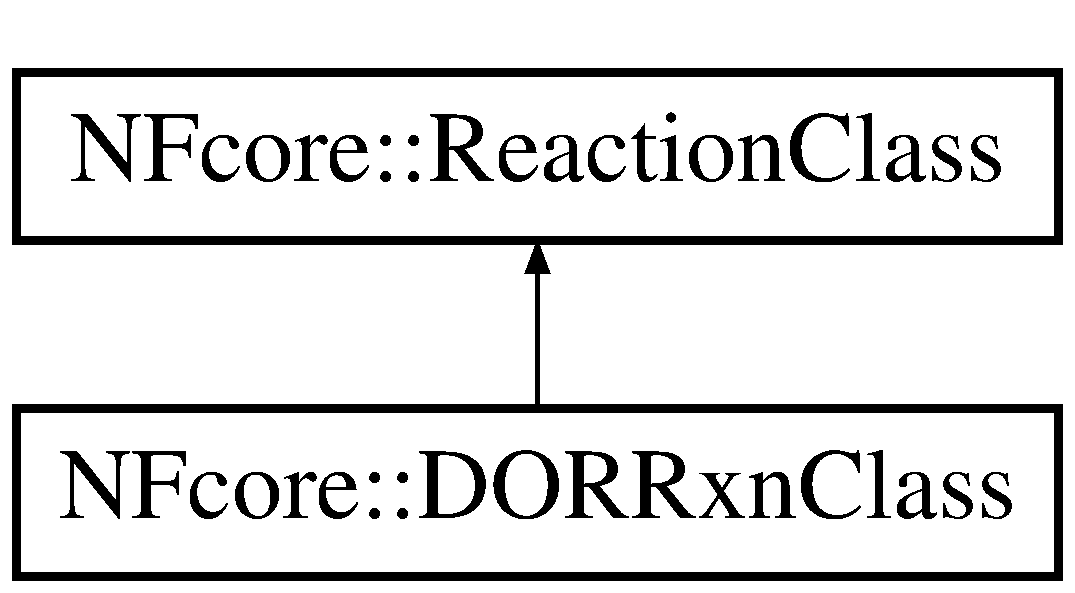
\includegraphics[height=2cm]{classNFcore_1_1DORRxnClass}
\end{center}
\end{figure}
\subsection*{Public Member Functions}
\begin{CompactItemize}
\item 
{\bf DORRxnClass} (string {\bf name}, double {\bf baseRate}, string baseRateName, {\bf TransformationSet} $\ast${\bf transformationSet}, {\bf CompositeFunction} $\ast$function, vector$<$ string $>$ \&lfArgumentPointerNameList, {\bf System} $\ast$s)
\item 
virtual {\bf $\sim$DORRxnClass} ()
\item 
virtual void {\bf init} ()
\item 
virtual void {\bf prepareForSimulation} ()
\item 
virtual bool {\bf tryToAdd} ({\bf Molecule} $\ast$m, unsigned int reactantPos)
\item 
virtual void {\bf remove} ({\bf Molecule} $\ast$m, unsigned int reactantPos)
\item 
virtual double {\bf update\_\-a} ()
\item 
virtual int {\bf getDORreactantPosition} () const 
\item 
virtual void {\bf notifyRateFactorChange} ({\bf Molecule} $\ast$m, int reactantIndex, int rxnListIndex)
\item 
virtual unsigned int {\bf getReactantCount} (unsigned int reactantIndex) const 
\item 
virtual void {\bf printDetails} () const 
\item 
virtual void {\bf printFullDetails} () const 
\item 
void {\bf directAddForDebugging} ({\bf Molecule} $\ast$m)
\item 
void {\bf printTreeForDebugging} ()
\end{CompactItemize}
\subsection*{Static Public Member Functions}
\begin{CompactItemize}
\item 
static void {\bf test1} ({\bf System} $\ast$s)
\end{CompactItemize}
\subsection*{Protected Member Functions}
\begin{CompactItemize}
\item 
virtual double {\bf evaluateLocalFunctions} ({\bf MappingSet} $\ast${\bf ms})
\item 
virtual void {\bf pickMappingSets} (double randNumber) const 
\end{CompactItemize}
\subsection*{Protected Attributes}
\begin{CompactItemize}
\item 
{\bf ReactantList} $\ast$$\ast$ {\bf reactantLists}
\item 
{\bf ReactantTree} $\ast$ {\bf reactantTree}
\item 
{\bf MappingSet} $\ast$ {\bf ms}
\item 
{\bf CompositeFunction} $\ast$ {\bf cf}
\item 
int {\bf DORreactantIndex}
\item 
int {\bf n\_\-argMolecules}
\item 
int $\ast$ {\bf argIndexIntoMappingSet}
\item 
{\bf Molecule} $\ast$$\ast$ {\bf argMappedMolecule}
\item 
int $\ast$ {\bf argScope}
\end{CompactItemize}


\subsection{Constructor \& Destructor Documentation}
\index{NFcore::DORRxnClass@{NFcore::DORRxnClass}!DORRxnClass@{DORRxnClass}}
\index{DORRxnClass@{DORRxnClass}!NFcore::DORRxnClass@{NFcore::DORRxnClass}}
\subsubsection{\setlength{\rightskip}{0pt plus 5cm}DORRxnClass::DORRxnClass (string {\em name}, double {\em baseRate}, string {\em baseRateName}, {\bf TransformationSet} $\ast$ {\em transformationSet}, {\bf CompositeFunction} $\ast$ {\em function}, vector$<$ string $>$ \& {\em lfArgumentPointerNameList}, {\bf System} $\ast$ {\em s})}\label{classNFcore_1_1DORRxnClass_25c5f2cfc17da0c52108bc216bb9b0d4}




Step 3: Wheh! now we can finally get on the business of creating the reactant lists and the reactant tree and setting the usual reactionClass parameters \index{NFcore::DORRxnClass@{NFcore::DORRxnClass}!$\sim$DORRxnClass@{$\sim$DORRxnClass}}
\index{$\sim$DORRxnClass@{$\sim$DORRxnClass}!NFcore::DORRxnClass@{NFcore::DORRxnClass}}
\subsubsection{\setlength{\rightskip}{0pt plus 5cm}DORRxnClass::$\sim$DORRxnClass ()\hspace{0.3cm}{\tt  [virtual]}}\label{classNFcore_1_1DORRxnClass_7b178d5f4595a551a4da7c64f9678454}




\subsection{Member Function Documentation}
\index{NFcore::DORRxnClass@{NFcore::DORRxnClass}!init@{init}}
\index{init@{init}!NFcore::DORRxnClass@{NFcore::DORRxnClass}}
\subsubsection{\setlength{\rightskip}{0pt plus 5cm}void DORRxnClass::init ()\hspace{0.3cm}{\tt  [virtual]}}\label{classNFcore_1_1DORRxnClass_bd3127e922a51881509c4958e46fc56f}




Implements {\bf NFcore::ReactionClass} \doxyref{}{p.}{classNFcore_1_1ReactionClass_fa3006801b4fcf821358bfca9bab8aa1}.\index{NFcore::DORRxnClass@{NFcore::DORRxnClass}!prepareForSimulation@{prepareForSimulation}}
\index{prepareForSimulation@{prepareForSimulation}!NFcore::DORRxnClass@{NFcore::DORRxnClass}}
\subsubsection{\setlength{\rightskip}{0pt plus 5cm}virtual void NFcore::DORRxnClass::prepareForSimulation ()\hspace{0.3cm}{\tt  [inline, virtual]}}\label{classNFcore_1_1DORRxnClass_afc1267a5cd558075d87f79837b3dcba}




Implements {\bf NFcore::ReactionClass} \doxyref{}{p.}{classNFcore_1_1ReactionClass_f6466927590b894478fbe765f4da8aad}.\index{NFcore::DORRxnClass@{NFcore::DORRxnClass}!tryToAdd@{tryToAdd}}
\index{tryToAdd@{tryToAdd}!NFcore::DORRxnClass@{NFcore::DORRxnClass}}
\subsubsection{\setlength{\rightskip}{0pt plus 5cm}bool DORRxnClass::tryToAdd ({\bf Molecule} $\ast$ {\em m}, unsigned int {\em reactantPos})\hspace{0.3cm}{\tt  [virtual]}}\label{classNFcore_1_1DORRxnClass_d766aeb571ab65fc188ef9fea8212384}




Implements {\bf NFcore::ReactionClass} \doxyref{}{p.}{classNFcore_1_1ReactionClass_7ef57431ab858d1039e9efedd011f1f0}.\index{NFcore::DORRxnClass@{NFcore::DORRxnClass}!remove@{remove}}
\index{remove@{remove}!NFcore::DORRxnClass@{NFcore::DORRxnClass}}
\subsubsection{\setlength{\rightskip}{0pt plus 5cm}void DORRxnClass::remove ({\bf Molecule} $\ast$ {\em m}, unsigned int {\em reactantPos})\hspace{0.3cm}{\tt  [virtual]}}\label{classNFcore_1_1DORRxnClass_724546efe978d79d53744567691bfd99}




Implements {\bf NFcore::ReactionClass} \doxyref{}{p.}{classNFcore_1_1ReactionClass_e9f356905524d6e370059b1e4ef5754a}.\index{NFcore::DORRxnClass@{NFcore::DORRxnClass}!update\_\-a@{update\_\-a}}
\index{update\_\-a@{update\_\-a}!NFcore::DORRxnClass@{NFcore::DORRxnClass}}
\subsubsection{\setlength{\rightskip}{0pt plus 5cm}double DORRxnClass::update\_\-a ()\hspace{0.3cm}{\tt  [virtual]}}\label{classNFcore_1_1DORRxnClass_077d5dc28b205d46a14d22487c08bb7e}




Implements {\bf NFcore::ReactionClass} \doxyref{}{p.}{classNFcore_1_1ReactionClass_f5aed18705e78d14bd1a8f82068add70}.\index{NFcore::DORRxnClass@{NFcore::DORRxnClass}!getDORreactantPosition@{getDORreactantPosition}}
\index{getDORreactantPosition@{getDORreactantPosition}!NFcore::DORRxnClass@{NFcore::DORRxnClass}}
\subsubsection{\setlength{\rightskip}{0pt plus 5cm}virtual int NFcore::DORRxnClass::getDORreactantPosition () const\hspace{0.3cm}{\tt  [inline, virtual]}}\label{classNFcore_1_1DORRxnClass_2a1fbaba84429f5b076ce40e1848cb65}




Reimplemented from {\bf NFcore::ReactionClass} \doxyref{}{p.}{classNFcore_1_1ReactionClass_06f85ae28c934c344542626c627929e7}.\index{NFcore::DORRxnClass@{NFcore::DORRxnClass}!notifyRateFactorChange@{notifyRateFactorChange}}
\index{notifyRateFactorChange@{notifyRateFactorChange}!NFcore::DORRxnClass@{NFcore::DORRxnClass}}
\subsubsection{\setlength{\rightskip}{0pt plus 5cm}void DORRxnClass::notifyRateFactorChange ({\bf Molecule} $\ast$ {\em m}, int {\em reactantIndex}, int {\em rxnListIndex})\hspace{0.3cm}{\tt  [virtual]}}\label{classNFcore_1_1DORRxnClass_ef4d5b83d7f268142af4bbb6c13f89b3}




Implements {\bf NFcore::ReactionClass} \doxyref{}{p.}{classNFcore_1_1ReactionClass_c18b82dc36c68699c00802201d7745cd}.\index{NFcore::DORRxnClass@{NFcore::DORRxnClass}!getReactantCount@{getReactantCount}}
\index{getReactantCount@{getReactantCount}!NFcore::DORRxnClass@{NFcore::DORRxnClass}}
\subsubsection{\setlength{\rightskip}{0pt plus 5cm}unsigned int DORRxnClass::getReactantCount (unsigned int {\em reactantIndex}) const\hspace{0.3cm}{\tt  [virtual]}}\label{classNFcore_1_1DORRxnClass_bff81c460e3398249e095f1f52a60652}




Implements {\bf NFcore::ReactionClass} \doxyref{}{p.}{classNFcore_1_1ReactionClass_a39fd321f4d58d79fa72812d65f1c762}.\index{NFcore::DORRxnClass@{NFcore::DORRxnClass}!printDetails@{printDetails}}
\index{printDetails@{printDetails}!NFcore::DORRxnClass@{NFcore::DORRxnClass}}
\subsubsection{\setlength{\rightskip}{0pt plus 5cm}void DORRxnClass::printDetails () const\hspace{0.3cm}{\tt  [virtual]}}\label{classNFcore_1_1DORRxnClass_9d90ba3fc8f0effd97f14080ed76b608}




Reimplemented from {\bf NFcore::ReactionClass} \doxyref{}{p.}{classNFcore_1_1ReactionClass_7944db14780627ea05cf290688a8bfd3}.\index{NFcore::DORRxnClass@{NFcore::DORRxnClass}!printFullDetails@{printFullDetails}}
\index{printFullDetails@{printFullDetails}!NFcore::DORRxnClass@{NFcore::DORRxnClass}}
\subsubsection{\setlength{\rightskip}{0pt plus 5cm}virtual void NFcore::DORRxnClass::printFullDetails () const\hspace{0.3cm}{\tt  [inline, virtual]}}\label{classNFcore_1_1DORRxnClass_25114f968aea64b0ba990ce58b974fb5}




Implements {\bf NFcore::ReactionClass} \doxyref{}{p.}{classNFcore_1_1ReactionClass_521a0b7a474568522bec973cfa6b5242}.\index{NFcore::DORRxnClass@{NFcore::DORRxnClass}!directAddForDebugging@{directAddForDebugging}}
\index{directAddForDebugging@{directAddForDebugging}!NFcore::DORRxnClass@{NFcore::DORRxnClass}}
\subsubsection{\setlength{\rightskip}{0pt plus 5cm}void NFcore::DORRxnClass::directAddForDebugging ({\bf Molecule} $\ast$ {\em m})}\label{classNFcore_1_1DORRxnClass_2d6fa883d31905b2206d13a4645c5d16}


\index{NFcore::DORRxnClass@{NFcore::DORRxnClass}!printTreeForDebugging@{printTreeForDebugging}}
\index{printTreeForDebugging@{printTreeForDebugging}!NFcore::DORRxnClass@{NFcore::DORRxnClass}}
\subsubsection{\setlength{\rightskip}{0pt plus 5cm}void NFcore::DORRxnClass::printTreeForDebugging ()}\label{classNFcore_1_1DORRxnClass_28618d0587e8a45d9d1cb1d0386018be}


\index{NFcore::DORRxnClass@{NFcore::DORRxnClass}!test1@{test1}}
\index{test1@{test1}!NFcore::DORRxnClass@{NFcore::DORRxnClass}}
\subsubsection{\setlength{\rightskip}{0pt plus 5cm}static void NFcore::DORRxnClass::test1 ({\bf System} $\ast$ {\em s})\hspace{0.3cm}{\tt  [static]}}\label{classNFcore_1_1DORRxnClass_717fc90c30d02d0968886af251927170}


\index{NFcore::DORRxnClass@{NFcore::DORRxnClass}!evaluateLocalFunctions@{evaluateLocalFunctions}}
\index{evaluateLocalFunctions@{evaluateLocalFunctions}!NFcore::DORRxnClass@{NFcore::DORRxnClass}}
\subsubsection{\setlength{\rightskip}{0pt plus 5cm}double DORRxnClass::evaluateLocalFunctions ({\bf MappingSet} $\ast$ {\em ms})\hspace{0.3cm}{\tt  [protected, virtual]}}\label{classNFcore_1_1DORRxnClass_be0c6a9d9313d5ab383056373993c315}


\index{NFcore::DORRxnClass@{NFcore::DORRxnClass}!pickMappingSets@{pickMappingSets}}
\index{pickMappingSets@{pickMappingSets}!NFcore::DORRxnClass@{NFcore::DORRxnClass}}
\subsubsection{\setlength{\rightskip}{0pt plus 5cm}void DORRxnClass::pickMappingSets (double {\em randNumber}) const\hspace{0.3cm}{\tt  [protected, virtual]}}\label{classNFcore_1_1DORRxnClass_5d5d078d2a84602132b708a9bcfb078f}




Implements {\bf NFcore::ReactionClass} \doxyref{}{p.}{classNFcore_1_1ReactionClass_ff3336a876f9e81904ee2b7be86bbdc5}.

\subsection{Member Data Documentation}
\index{NFcore::DORRxnClass@{NFcore::DORRxnClass}!reactantLists@{reactantLists}}
\index{reactantLists@{reactantLists}!NFcore::DORRxnClass@{NFcore::DORRxnClass}}
\subsubsection{\setlength{\rightskip}{0pt plus 5cm}{\bf ReactantList}$\ast$$\ast$ {\bf NFcore::DORRxnClass::reactantLists}\hspace{0.3cm}{\tt  [protected]}}\label{classNFcore_1_1DORRxnClass_3bf2edf9e3727570ed40bd78981a436d}


\index{NFcore::DORRxnClass@{NFcore::DORRxnClass}!reactantTree@{reactantTree}}
\index{reactantTree@{reactantTree}!NFcore::DORRxnClass@{NFcore::DORRxnClass}}
\subsubsection{\setlength{\rightskip}{0pt plus 5cm}{\bf ReactantTree}$\ast$ {\bf NFcore::DORRxnClass::reactantTree}\hspace{0.3cm}{\tt  [protected]}}\label{classNFcore_1_1DORRxnClass_0092e4152b63564ac4bdbe7483f75ee9}


\index{NFcore::DORRxnClass@{NFcore::DORRxnClass}!ms@{ms}}
\index{ms@{ms}!NFcore::DORRxnClass@{NFcore::DORRxnClass}}
\subsubsection{\setlength{\rightskip}{0pt plus 5cm}{\bf MappingSet}$\ast$ {\bf NFcore::DORRxnClass::ms}\hspace{0.3cm}{\tt  [protected]}}\label{classNFcore_1_1DORRxnClass_aa697478dd241353c26cb95cab98465d}


\index{NFcore::DORRxnClass@{NFcore::DORRxnClass}!cf@{cf}}
\index{cf@{cf}!NFcore::DORRxnClass@{NFcore::DORRxnClass}}
\subsubsection{\setlength{\rightskip}{0pt plus 5cm}{\bf CompositeFunction}$\ast$ {\bf NFcore::DORRxnClass::cf}\hspace{0.3cm}{\tt  [protected]}}\label{classNFcore_1_1DORRxnClass_2e39204468b229554071b066e895eba6}


\index{NFcore::DORRxnClass@{NFcore::DORRxnClass}!DORreactantIndex@{DORreactantIndex}}
\index{DORreactantIndex@{DORreactantIndex}!NFcore::DORRxnClass@{NFcore::DORRxnClass}}
\subsubsection{\setlength{\rightskip}{0pt plus 5cm}int {\bf NFcore::DORRxnClass::DORreactantIndex}\hspace{0.3cm}{\tt  [protected]}}\label{classNFcore_1_1DORRxnClass_093d9bdb7894f01306b18e7106c5401e}


\index{NFcore::DORRxnClass@{NFcore::DORRxnClass}!n\_\-argMolecules@{n\_\-argMolecules}}
\index{n\_\-argMolecules@{n\_\-argMolecules}!NFcore::DORRxnClass@{NFcore::DORRxnClass}}
\subsubsection{\setlength{\rightskip}{0pt plus 5cm}int {\bf NFcore::DORRxnClass::n\_\-argMolecules}\hspace{0.3cm}{\tt  [protected]}}\label{classNFcore_1_1DORRxnClass_fc6737775a1fc8abf8cceef9ae5446d5}


\index{NFcore::DORRxnClass@{NFcore::DORRxnClass}!argIndexIntoMappingSet@{argIndexIntoMappingSet}}
\index{argIndexIntoMappingSet@{argIndexIntoMappingSet}!NFcore::DORRxnClass@{NFcore::DORRxnClass}}
\subsubsection{\setlength{\rightskip}{0pt plus 5cm}int$\ast$ {\bf NFcore::DORRxnClass::argIndexIntoMappingSet}\hspace{0.3cm}{\tt  [protected]}}\label{classNFcore_1_1DORRxnClass_a9ca0a270fd943c2b8a1036f585fd9c3}


\index{NFcore::DORRxnClass@{NFcore::DORRxnClass}!argMappedMolecule@{argMappedMolecule}}
\index{argMappedMolecule@{argMappedMolecule}!NFcore::DORRxnClass@{NFcore::DORRxnClass}}
\subsubsection{\setlength{\rightskip}{0pt plus 5cm}{\bf Molecule}$\ast$$\ast$ {\bf NFcore::DORRxnClass::argMappedMolecule}\hspace{0.3cm}{\tt  [protected]}}\label{classNFcore_1_1DORRxnClass_2d317bf00f8b9a01236ffe2a602c9b98}


\index{NFcore::DORRxnClass@{NFcore::DORRxnClass}!argScope@{argScope}}
\index{argScope@{argScope}!NFcore::DORRxnClass@{NFcore::DORRxnClass}}
\subsubsection{\setlength{\rightskip}{0pt plus 5cm}int$\ast$ {\bf NFcore::DORRxnClass::argScope}\hspace{0.3cm}{\tt  [protected]}}\label{classNFcore_1_1DORRxnClass_002aa17c5b8c6a85ed045a09f32994fa}




The documentation for this class was generated from the following files:\begin{CompactItemize}
\item 
/home/msneddon/eclipse/indigo/workspace/NFsim/src/NFreactions/reactions/{\bf reaction.hh}\item 
/home/msneddon/eclipse/indigo/workspace/NFsim/src/NFreactions/reactions/{\bf DORreaction.cpp}\end{CompactItemize}

\section{NFcore::DumpAllComplexes Class Reference}
\label{classNFcore_1_1DumpAllComplexes}\index{NFcore::DumpAllComplexes@{NFcore::DumpAllComplexes}}
{\tt \#include $<$NFoutput.hh$>$}

Inheritance diagram for NFcore::DumpAllComplexes::\begin{figure}[H]
\begin{center}
\leavevmode
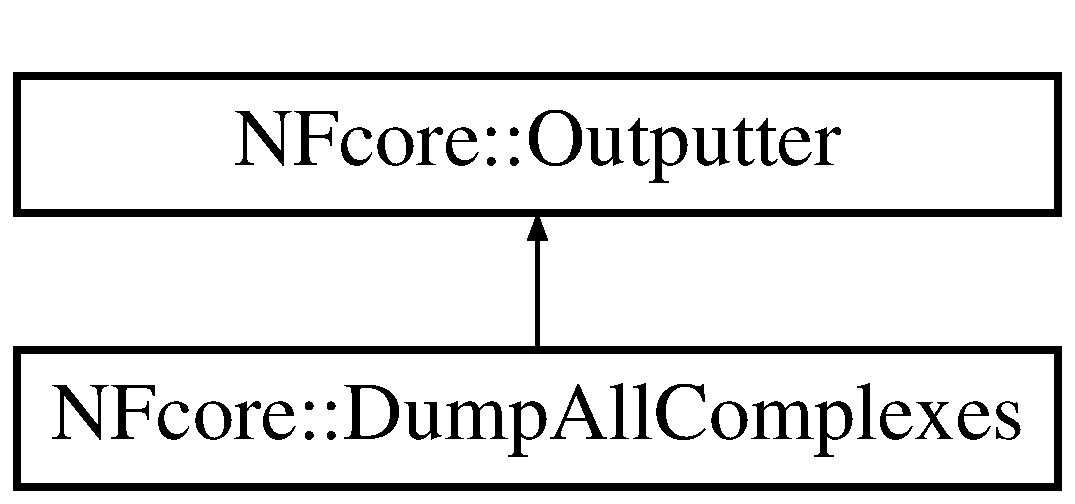
\includegraphics[height=2cm]{classNFcore_1_1DumpAllComplexes}
\end{center}
\end{figure}
\subsection*{Public Member Functions}
\begin{CompactItemize}
\item 
{\bf DumpAllComplexes} (string {\bf filename}, {\bf System} $\ast${\bf s})
\item 
virtual {\bf $\sim$DumpAllComplexes} ()
\item 
virtual void {\bf output} ()
\item 
virtual void {\bf outputHeader} ()
\item 
virtual void {\bf tryToDump} (double simTime)
\end{CompactItemize}
\subsection*{Protected Attributes}
\begin{CompactItemize}
\item 
{\bf MoleculeType} $\ast$ {\bf mt}
\end{CompactItemize}


\subsection{Constructor \& Destructor Documentation}
\index{NFcore::DumpAllComplexes@{NFcore::DumpAllComplexes}!DumpAllComplexes@{DumpAllComplexes}}
\index{DumpAllComplexes@{DumpAllComplexes}!NFcore::DumpAllComplexes@{NFcore::DumpAllComplexes}}
\subsubsection{\setlength{\rightskip}{0pt plus 5cm}NFcore::DumpAllComplexes::DumpAllComplexes (string {\em filename}, {\bf System} $\ast$ {\em s})}\label{classNFcore_1_1DumpAllComplexes_1a066d6f29e3980d37290b94c635f3f8}


\index{NFcore::DumpAllComplexes@{NFcore::DumpAllComplexes}!$\sim$DumpAllComplexes@{$\sim$DumpAllComplexes}}
\index{$\sim$DumpAllComplexes@{$\sim$DumpAllComplexes}!NFcore::DumpAllComplexes@{NFcore::DumpAllComplexes}}
\subsubsection{\setlength{\rightskip}{0pt plus 5cm}virtual NFcore::DumpAllComplexes::$\sim$DumpAllComplexes ()\hspace{0.3cm}{\tt  [virtual]}}\label{classNFcore_1_1DumpAllComplexes_fe36ab7a691bfe15900034e0fdcd90ff}




\subsection{Member Function Documentation}
\index{NFcore::DumpAllComplexes@{NFcore::DumpAllComplexes}!output@{output}}
\index{output@{output}!NFcore::DumpAllComplexes@{NFcore::DumpAllComplexes}}
\subsubsection{\setlength{\rightskip}{0pt plus 5cm}virtual void NFcore::DumpAllComplexes::output ()\hspace{0.3cm}{\tt  [virtual]}}\label{classNFcore_1_1DumpAllComplexes_954c5b398a98f2a238b0318c28b5569b}




Implements {\bf NFcore::Outputter} \doxyref{}{p.}{classNFcore_1_1Outputter_fa0b98db6598c1d00b143b61f0c5c575}.\index{NFcore::DumpAllComplexes@{NFcore::DumpAllComplexes}!outputHeader@{outputHeader}}
\index{outputHeader@{outputHeader}!NFcore::DumpAllComplexes@{NFcore::DumpAllComplexes}}
\subsubsection{\setlength{\rightskip}{0pt plus 5cm}virtual void NFcore::DumpAllComplexes::outputHeader ()\hspace{0.3cm}{\tt  [virtual]}}\label{classNFcore_1_1DumpAllComplexes_32dfb2527b4702cade795b224773caaa}




Implements {\bf NFcore::Outputter} \doxyref{}{p.}{classNFcore_1_1Outputter_14be13a01fc8c5c515bf4ddb8b721e3c}.\index{NFcore::DumpAllComplexes@{NFcore::DumpAllComplexes}!tryToDump@{tryToDump}}
\index{tryToDump@{tryToDump}!NFcore::DumpAllComplexes@{NFcore::DumpAllComplexes}}
\subsubsection{\setlength{\rightskip}{0pt plus 5cm}virtual void NFcore::DumpAllComplexes::tryToDump (double {\em simTime})\hspace{0.3cm}{\tt  [virtual]}}\label{classNFcore_1_1DumpAllComplexes_2e6c3d41d2d294a786e5f4f6ce236b39}




Implements {\bf NFcore::Outputter} \doxyref{}{p.}{classNFcore_1_1Outputter_f6476687694630364712b462afea04e6}.

\subsection{Member Data Documentation}
\index{NFcore::DumpAllComplexes@{NFcore::DumpAllComplexes}!mt@{mt}}
\index{mt@{mt}!NFcore::DumpAllComplexes@{NFcore::DumpAllComplexes}}
\subsubsection{\setlength{\rightskip}{0pt plus 5cm}{\bf MoleculeType}$\ast$ {\bf NFcore::DumpAllComplexes::mt}\hspace{0.3cm}{\tt  [protected]}}\label{classNFcore_1_1DumpAllComplexes_511824e0bed32ec4abdfdf5933446df8}




The documentation for this class was generated from the following file:\begin{CompactItemize}
\item 
/home/msneddon/eclipse/ganymede\_\-cpp/workspace/NFsim\_\-svn/src/NFoutput/{\bf NFoutput.hh}\end{CompactItemize}

\section{NFcore::DumpMoleculeType Class Reference}
\label{classNFcore_1_1DumpMoleculeType}\index{NFcore::DumpMoleculeType@{NFcore::DumpMoleculeType}}
{\tt \#include $<$NFoutput.hh$>$}

Inheritance diagram for NFcore::DumpMoleculeType::\begin{figure}[H]
\begin{center}
\leavevmode
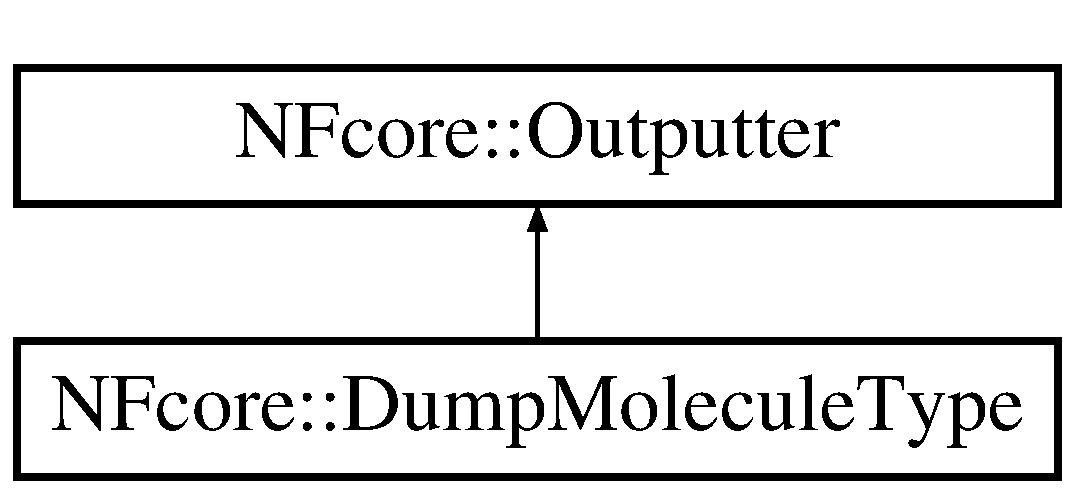
\includegraphics[height=2cm]{classNFcore_1_1DumpMoleculeType}
\end{center}
\end{figure}
\subsection*{Public Member Functions}
\begin{CompactItemize}
\item 
{\bf DumpMoleculeType} (string {\bf filename}, {\bf System} $\ast${\bf s}, {\bf MoleculeType} $\ast${\bf mt})
\item 
virtual {\bf $\sim$DumpMoleculeType} ()
\item 
virtual void {\bf output} ()
\item 
virtual void {\bf outputHeader} ()
\end{CompactItemize}
\subsection*{Protected Attributes}
\begin{CompactItemize}
\item 
{\bf MoleculeType} $\ast$ {\bf mt}
\end{CompactItemize}


\subsection{Constructor \& Destructor Documentation}
\index{NFcore::DumpMoleculeType@{NFcore::DumpMoleculeType}!DumpMoleculeType@{DumpMoleculeType}}
\index{DumpMoleculeType@{DumpMoleculeType}!NFcore::DumpMoleculeType@{NFcore::DumpMoleculeType}}
\subsubsection{\setlength{\rightskip}{0pt plus 5cm}DumpMoleculeType::DumpMoleculeType (string {\em filename}, {\bf System} $\ast$ {\em s}, {\bf MoleculeType} $\ast$ {\em mt})}\label{classNFcore_1_1DumpMoleculeType_9a98e25a2798cf852528babe4ace5ed6}


\index{NFcore::DumpMoleculeType@{NFcore::DumpMoleculeType}!$\sim$DumpMoleculeType@{$\sim$DumpMoleculeType}}
\index{$\sim$DumpMoleculeType@{$\sim$DumpMoleculeType}!NFcore::DumpMoleculeType@{NFcore::DumpMoleculeType}}
\subsubsection{\setlength{\rightskip}{0pt plus 5cm}DumpMoleculeType::$\sim$DumpMoleculeType ()\hspace{0.3cm}{\tt  [virtual]}}\label{classNFcore_1_1DumpMoleculeType_ddc87564aad207ea6418c70b9eafd832}




\subsection{Member Function Documentation}
\index{NFcore::DumpMoleculeType@{NFcore::DumpMoleculeType}!output@{output}}
\index{output@{output}!NFcore::DumpMoleculeType@{NFcore::DumpMoleculeType}}
\subsubsection{\setlength{\rightskip}{0pt plus 5cm}void DumpMoleculeType::output ()\hspace{0.3cm}{\tt  [virtual]}}\label{classNFcore_1_1DumpMoleculeType_22126e4f9c628dc8952f17ef48980d7e}




Implements {\bf NFcore::Outputter} \doxyref{}{p.}{classNFcore_1_1Outputter_fa0b98db6598c1d00b143b61f0c5c575}.\index{NFcore::DumpMoleculeType@{NFcore::DumpMoleculeType}!outputHeader@{outputHeader}}
\index{outputHeader@{outputHeader}!NFcore::DumpMoleculeType@{NFcore::DumpMoleculeType}}
\subsubsection{\setlength{\rightskip}{0pt plus 5cm}void DumpMoleculeType::outputHeader ()\hspace{0.3cm}{\tt  [virtual]}}\label{classNFcore_1_1DumpMoleculeType_89a0e8fdbfca05907019a42b2ebd13f4}




Implements {\bf NFcore::Outputter} \doxyref{}{p.}{classNFcore_1_1Outputter_14be13a01fc8c5c515bf4ddb8b721e3c}.

\subsection{Member Data Documentation}
\index{NFcore::DumpMoleculeType@{NFcore::DumpMoleculeType}!mt@{mt}}
\index{mt@{mt}!NFcore::DumpMoleculeType@{NFcore::DumpMoleculeType}}
\subsubsection{\setlength{\rightskip}{0pt plus 5cm}{\bf MoleculeType}$\ast$ {\bf NFcore::DumpMoleculeType::mt}\hspace{0.3cm}{\tt  [protected]}}\label{classNFcore_1_1DumpMoleculeType_e624fa39a020b70a56c257cef5256120}




The documentation for this class was generated from the following files:\begin{CompactItemize}
\item 
/home/msneddon/eclipse/ganymede\_\-cpp/workspace/NFsim\_\-svn/src/NFoutput/{\bf NFoutput.hh}\item 
/home/msneddon/eclipse/ganymede\_\-cpp/workspace/NFsim\_\-svn/src/NFoutput/{\bf NFoutput.cpp}\end{CompactItemize}

\section{NFcore::EmptyTransform Class Reference}
\label{classNFcore_1_1EmptyTransform}\index{NFcore::EmptyTransform@{NFcore::EmptyTransform}}
{\tt \#include $<$transformation.hh$>$}

Inheritance diagram for NFcore::EmptyTransform::\begin{figure}[H]
\begin{center}
\leavevmode
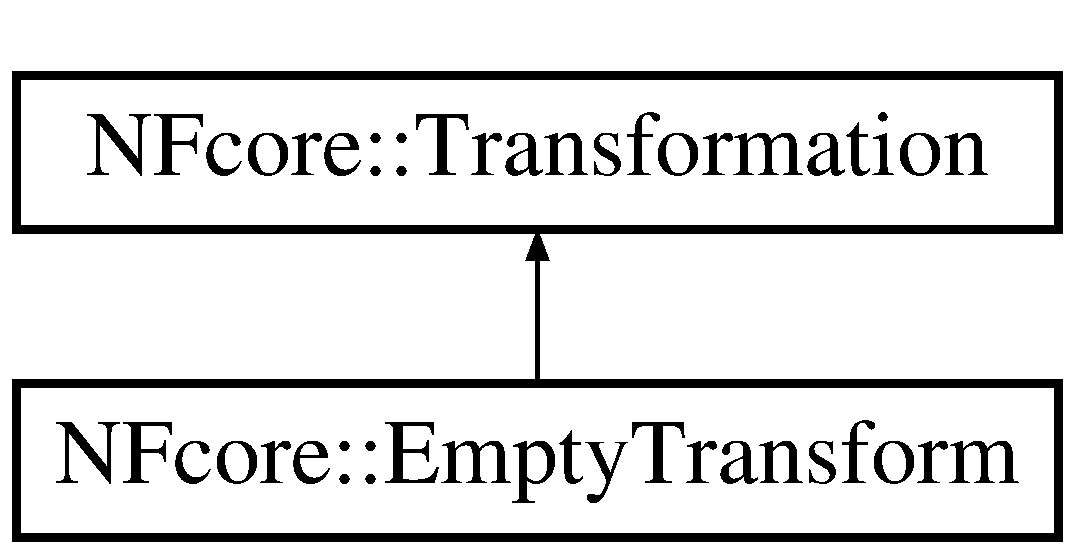
\includegraphics[height=2cm]{classNFcore_1_1EmptyTransform}
\end{center}
\end{figure}
\subsection*{Public Member Functions}
\begin{CompactItemize}
\item 
{\bf EmptyTransform} ()
\item 
{\bf EmptyTransform} (int {\bf cIndex})
\item 
virtual {\bf $\sim$EmptyTransform} ()
\item 
virtual void {\bf apply} ({\bf Mapping} $\ast$m, {\bf MappingSet} $\ast$$\ast$ms)
\item 
virtual int {\bf getComponentIndex} () const 
\end{CompactItemize}
\subsection*{Protected Attributes}
\begin{CompactItemize}
\item 
int {\bf cIndex}
\end{CompactItemize}


\subsection{Constructor \& Destructor Documentation}
\index{NFcore::EmptyTransform@{NFcore::EmptyTransform}!EmptyTransform@{EmptyTransform}}
\index{EmptyTransform@{EmptyTransform}!NFcore::EmptyTransform@{NFcore::EmptyTransform}}
\subsubsection{\setlength{\rightskip}{0pt plus 5cm}NFcore::EmptyTransform::EmptyTransform ()\hspace{0.3cm}{\tt  [inline]}}\label{classNFcore_1_1EmptyTransform_d88722275fb2bc1cb272f95138eb8441}


\index{NFcore::EmptyTransform@{NFcore::EmptyTransform}!EmptyTransform@{EmptyTransform}}
\index{EmptyTransform@{EmptyTransform}!NFcore::EmptyTransform@{NFcore::EmptyTransform}}
\subsubsection{\setlength{\rightskip}{0pt plus 5cm}NFcore::EmptyTransform::EmptyTransform (int {\em cIndex})\hspace{0.3cm}{\tt  [inline]}}\label{classNFcore_1_1EmptyTransform_1a2a573b650d8c1ffe9c99acbb9b5660}


\index{NFcore::EmptyTransform@{NFcore::EmptyTransform}!$\sim$EmptyTransform@{$\sim$EmptyTransform}}
\index{$\sim$EmptyTransform@{$\sim$EmptyTransform}!NFcore::EmptyTransform@{NFcore::EmptyTransform}}
\subsubsection{\setlength{\rightskip}{0pt plus 5cm}virtual NFcore::EmptyTransform::$\sim$EmptyTransform ()\hspace{0.3cm}{\tt  [inline, virtual]}}\label{classNFcore_1_1EmptyTransform_a0800f7a7a71c85e712dfdc7319aaeb4}




\subsection{Member Function Documentation}
\index{NFcore::EmptyTransform@{NFcore::EmptyTransform}!apply@{apply}}
\index{apply@{apply}!NFcore::EmptyTransform@{NFcore::EmptyTransform}}
\subsubsection{\setlength{\rightskip}{0pt plus 5cm}virtual void NFcore::EmptyTransform::apply ({\bf Mapping} $\ast$ {\em m}, {\bf MappingSet} $\ast$$\ast$ {\em ms})\hspace{0.3cm}{\tt  [inline, virtual]}}\label{classNFcore_1_1EmptyTransform_fd2dd5c89bfd563a2343a9a40a3a21b1}




Implements {\bf NFcore::Transformation} \doxyref{}{p.}{classNFcore_1_1Transformation_6a57f607676c92b2465427e57bc7fae5}.\index{NFcore::EmptyTransform@{NFcore::EmptyTransform}!getComponentIndex@{getComponentIndex}}
\index{getComponentIndex@{getComponentIndex}!NFcore::EmptyTransform@{NFcore::EmptyTransform}}
\subsubsection{\setlength{\rightskip}{0pt plus 5cm}virtual int NFcore::EmptyTransform::getComponentIndex () const\hspace{0.3cm}{\tt  [inline, virtual]}}\label{classNFcore_1_1EmptyTransform_7263f704ef8b0fe2388da3379880df4d}




Implements {\bf NFcore::Transformation} \doxyref{}{p.}{classNFcore_1_1Transformation_2ba394b20768b21ba328431103474607}.

\subsection{Member Data Documentation}
\index{NFcore::EmptyTransform@{NFcore::EmptyTransform}!cIndex@{cIndex}}
\index{cIndex@{cIndex}!NFcore::EmptyTransform@{NFcore::EmptyTransform}}
\subsubsection{\setlength{\rightskip}{0pt plus 5cm}int {\bf NFcore::EmptyTransform::cIndex}\hspace{0.3cm}{\tt  [protected]}}\label{classNFcore_1_1EmptyTransform_08e0951a5896aae457efdc44b51143b1}




The documentation for this class was generated from the following file:\begin{CompactItemize}
\item 
/home/msneddon/eclipse/indigo/workspace/NFsim/src/NFreactions/transformations/{\bf transformation.hh}\end{CompactItemize}

\section{NFcore::FuncFactory Class Reference}
\label{classNFcore_1_1FuncFactory}\index{NFcore::FuncFactory@{NFcore::FuncFactory}}
{\tt \#include $<$NFfunction.hh$>$}



\subsection{Detailed Description}
Parses mathmatical functions that can be easily used anywhere. 

Built from the muParser freeware package, this factory creates Parser objects that can be used to evaluate arbitrary functions. The function to evaluate is given as a string (which can contain the given functions or constants below, case sensitive) along with pointers to particular varables that exist. The Parser, when initialized, translates the string into bytecode that can be evaluated fast. At runtime, the bytecode that was created can be evaluated and every time it is evaluated, it uses the current value of the given pointers to variables. Thus, NFsim can use functions of arbitrary complexity for defining reaction rates and parameters.

{\bf Supported functions:} \begin{TabularC}{3}
\hline
name\&nbsp\&nbsp&n\_\-args\&nbsp\&nbsp&description \\\hline
sin&1&sine function (arg is in radians) \\\hline
cos&1&cosine function \\\hline
tan&1&tangens function \\\hline
asin&1&arcus sine function \\\hline
acos&1&arcus cosine function \\\hline
atan&1&arcus tangens function \\\hline
sinh&1&hyperbolic sine function \\\hline
cosh&1&hyperbolic cosine \\\hline
tanh&1&hyperbolic tangens function \\\hline
asinh&1&hyperbolic arcus sine function \\\hline
acosh&1&hyperbolic arcus tangens function \\\hline
atanh&1&hyperbolic arcur tangens function \\\hline
log2&1&logarithm to the base 2 \\\hline
log10&1&logarithm to the base 10 \\\hline
log&1&logarithm to the base 10 \\\hline
ln&1&logarithm to base e (2.71828...) \\\hline
exp&1&e raised to the power of x \\\hline
sqrt&1&square root of a value \\\hline
sign&1&sign function -1 if x$<$0; 1 if x$>$0 \\\hline
rint&1&round to nearest integer \\\hline
abs&1&absolute value \\\hline
if&3&if ... then ... else ... \\\hline
min&var.&min of all arguments \\\hline
max&var.&max of all arguments \\\hline
sum&var.&sum of all arguments \\\hline
avg&var.&mean value of all arguments \\\hline
\end{TabularC}


{\bf Supported constants} (to a precision of at least 10$^\wedge$-8): \begin{TabularC}{3}
\hline
name\&nbsp\&nbsp&value\&nbsp\&nbsp&description \\\hline
\_\-PI&3.141...&you all know pi, right? \\\hline
\_\-e&2.718...&the base of natural logs \\\hline
\_\-Na&6.022...e23&Avogadro's number \\\hline
\end{TabularC}


For muParser documentation, see: {\tt http://muparser.sourceforge.net/} \subsection*{Static Public Member Functions}
\begin{CompactItemize}
\item 
static mu::Parser $\ast$ {\bf create} (string function, vector$<$ string $>$ \&variableNames, vector$<$ double $\ast$ $>$ \&variablePtrs)
\item 
static mu::Parser $\ast$ {\bf create} ()
\item 
static double {\bf Eval} (mu::Parser $\ast$p)
\item 
static void {\bf test} ()
\end{CompactItemize}


\subsection{Member Function Documentation}
\index{NFcore::FuncFactory@{NFcore::FuncFactory}!create@{create}}
\index{create@{create}!NFcore::FuncFactory@{NFcore::FuncFactory}}
\subsubsection{\setlength{\rightskip}{0pt plus 5cm}Parser $\ast$ FuncFactory::create (string {\em function}, vector$<$ string $>$ \& {\em variableNames}, vector$<$ double $\ast$ $>$ \& {\em variablePtrs})\hspace{0.3cm}{\tt  [static]}}\label{classNFcore_1_1FuncFactory_77b38df3330c3b4b9247e55377016da4}


Use this function to create a new function parser that can operate on the given variables. The vectors should contain (in the same order) the variable names and pointers to the actual variable values. Do not use local variables or variables that will be forgotten before the Parser is destroyed. To evaluate functions, you can either just call the \doxyref{Eval()}{p.}{classNFcore_1_1FuncFactory_31bc4b8afdd056b59e80e55dbd28715a} function of the Parser object (as in p-$>$\doxyref{Eval()}{p.}{classNFcore_1_1FuncFactory_31bc4b8afdd056b59e80e55dbd28715a}), or, call the Eval function of \doxyref{FuncFactory}{p.}{classNFcore_1_1FuncFactory} to do error checking (as in FuncFactory::Eval(p)). \index{NFcore::FuncFactory@{NFcore::FuncFactory}!create@{create}}
\index{create@{create}!NFcore::FuncFactory@{NFcore::FuncFactory}}
\subsubsection{\setlength{\rightskip}{0pt plus 5cm}Parser $\ast$ FuncFactory::create ()\hspace{0.3cm}{\tt  [static]}}\label{classNFcore_1_1FuncFactory_06027d4126ce96a32c7ce001ad7cb733}


Creates a function without any variables and without any functions defined. You will have to do that yourself. But, this does add in any predefined constants we want, and that is why this function exists. \index{NFcore::FuncFactory@{NFcore::FuncFactory}!Eval@{Eval}}
\index{Eval@{Eval}!NFcore::FuncFactory@{NFcore::FuncFactory}}
\subsubsection{\setlength{\rightskip}{0pt plus 5cm}double FuncFactory::Eval (mu::Parser $\ast$ {\em p})\hspace{0.3cm}{\tt  [static]}}\label{classNFcore_1_1FuncFactory_31bc4b8afdd056b59e80e55dbd28715a}


Evaluates the given Parser object safely, meaning exceptions and errors are caught and program execution is terminated - if you have to do better than simple program termination, well than you can catch your own errors (see the muParser documenation). \index{NFcore::FuncFactory@{NFcore::FuncFactory}!test@{test}}
\index{test@{test}!NFcore::FuncFactory@{NFcore::FuncFactory}}
\subsubsection{\setlength{\rightskip}{0pt plus 5cm}void FuncFactory::test ()\hspace{0.3cm}{\tt  [static]}}\label{classNFcore_1_1FuncFactory_e3bba8b455353e58dabe2add83a1aeae}


Runs a couple tests of the \doxyref{FuncFactory}{p.}{classNFcore_1_1FuncFactory} and the muParser functions to make sure everything is working as promised. (To run this, use the arguements '-test mathFuncParser') 

The documentation for this class was generated from the following files:\begin{CompactItemize}
\item 
/home/msneddon/eclipse/indigo/workspace/NFsim/src/NFfunction/{\bf NFfunction.hh}\item 
/home/msneddon/eclipse/indigo/workspace/NFsim/src/NFfunction/{\bf funcParser.cpp}\end{CompactItemize}

\section{NFcore::FunctionalRxnClass Class Reference}
\label{classNFcore_1_1FunctionalRxnClass}\index{NFcore::FunctionalRxnClass@{NFcore::FunctionalRxnClass}}
{\tt \#include $<$reaction.hh$>$}

Inheritance diagram for NFcore::FunctionalRxnClass::\begin{figure}[H]
\begin{center}
\leavevmode
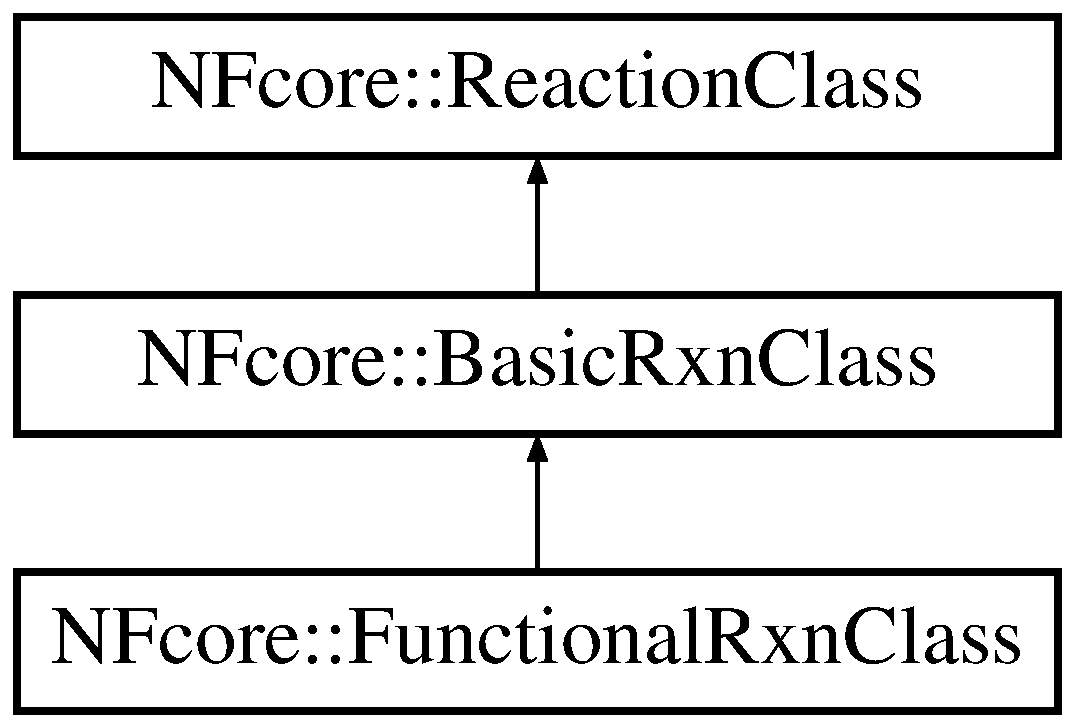
\includegraphics[height=3cm]{classNFcore_1_1FunctionalRxnClass}
\end{center}
\end{figure}
\subsection*{Public Member Functions}
\begin{CompactItemize}
\item 
{\bf FunctionalRxnClass} (string {\bf name}, {\bf GlobalFunction} $\ast${\bf gf}, {\bf TransformationSet} $\ast${\bf transformationSet}, {\bf System} $\ast$s)
\item 
{\bf FunctionalRxnClass} (string {\bf name}, {\bf CompositeFunction} $\ast${\bf cf}, {\bf TransformationSet} $\ast${\bf transformationSet}, {\bf System} $\ast$s)
\item 
virtual {\bf $\sim$FunctionalRxnClass} ()
\item 
virtual double {\bf update\_\-a} ()
\item 
virtual void {\bf printDetails} () const 
\end{CompactItemize}
\subsection*{Protected Attributes}
\begin{CompactItemize}
\item 
{\bf GlobalFunction} $\ast$ {\bf gf}
\item 
{\bf CompositeFunction} $\ast$ {\bf cf}
\end{CompactItemize}


\subsection{Constructor \& Destructor Documentation}
\index{NFcore::FunctionalRxnClass@{NFcore::FunctionalRxnClass}!FunctionalRxnClass@{FunctionalRxnClass}}
\index{FunctionalRxnClass@{FunctionalRxnClass}!NFcore::FunctionalRxnClass@{NFcore::FunctionalRxnClass}}
\subsubsection{\setlength{\rightskip}{0pt plus 5cm}FunctionalRxnClass::FunctionalRxnClass (string {\em name}, {\bf GlobalFunction} $\ast$ {\em gf}, {\bf TransformationSet} $\ast$ {\em transformationSet}, {\bf System} $\ast$ {\em s})}\label{classNFcore_1_1FunctionalRxnClass_d217200f15b7012404c2faedf6223d3c}


\index{NFcore::FunctionalRxnClass@{NFcore::FunctionalRxnClass}!FunctionalRxnClass@{FunctionalRxnClass}}
\index{FunctionalRxnClass@{FunctionalRxnClass}!NFcore::FunctionalRxnClass@{NFcore::FunctionalRxnClass}}
\subsubsection{\setlength{\rightskip}{0pt plus 5cm}FunctionalRxnClass::FunctionalRxnClass (string {\em name}, {\bf CompositeFunction} $\ast$ {\em cf}, {\bf TransformationSet} $\ast$ {\em transformationSet}, {\bf System} $\ast$ {\em s})}\label{classNFcore_1_1FunctionalRxnClass_5f169e961bea836542530f0a15676b14}


\index{NFcore::FunctionalRxnClass@{NFcore::FunctionalRxnClass}!$\sim$FunctionalRxnClass@{$\sim$FunctionalRxnClass}}
\index{$\sim$FunctionalRxnClass@{$\sim$FunctionalRxnClass}!NFcore::FunctionalRxnClass@{NFcore::FunctionalRxnClass}}
\subsubsection{\setlength{\rightskip}{0pt plus 5cm}FunctionalRxnClass::$\sim$FunctionalRxnClass ()\hspace{0.3cm}{\tt  [virtual]}}\label{classNFcore_1_1FunctionalRxnClass_a4d16f41264250be2ee9dd4749d90937}




\subsection{Member Function Documentation}
\index{NFcore::FunctionalRxnClass@{NFcore::FunctionalRxnClass}!update\_\-a@{update\_\-a}}
\index{update\_\-a@{update\_\-a}!NFcore::FunctionalRxnClass@{NFcore::FunctionalRxnClass}}
\subsubsection{\setlength{\rightskip}{0pt plus 5cm}double FunctionalRxnClass::update\_\-a ()\hspace{0.3cm}{\tt  [virtual]}}\label{classNFcore_1_1FunctionalRxnClass_23dd5630ec0157ce7ab6d240720a57cb}




Reimplemented from {\bf NFcore::BasicRxnClass} \doxyref{}{p.}{classNFcore_1_1BasicRxnClass_9a679d57f4cfdd184f3bf312ecd20cc6}.\index{NFcore::FunctionalRxnClass@{NFcore::FunctionalRxnClass}!printDetails@{printDetails}}
\index{printDetails@{printDetails}!NFcore::FunctionalRxnClass@{NFcore::FunctionalRxnClass}}
\subsubsection{\setlength{\rightskip}{0pt plus 5cm}void FunctionalRxnClass::printDetails () const\hspace{0.3cm}{\tt  [virtual]}}\label{classNFcore_1_1FunctionalRxnClass_54fa8f462e0d990d8b547892fca9b918}




Reimplemented from {\bf NFcore::ReactionClass} \doxyref{}{p.}{classNFcore_1_1ReactionClass_7944db14780627ea05cf290688a8bfd3}.

\subsection{Member Data Documentation}
\index{NFcore::FunctionalRxnClass@{NFcore::FunctionalRxnClass}!gf@{gf}}
\index{gf@{gf}!NFcore::FunctionalRxnClass@{NFcore::FunctionalRxnClass}}
\subsubsection{\setlength{\rightskip}{0pt plus 5cm}{\bf GlobalFunction}$\ast$ {\bf NFcore::FunctionalRxnClass::gf}\hspace{0.3cm}{\tt  [protected]}}\label{classNFcore_1_1FunctionalRxnClass_c795f335300c3e6023ae361767504978}


\index{NFcore::FunctionalRxnClass@{NFcore::FunctionalRxnClass}!cf@{cf}}
\index{cf@{cf}!NFcore::FunctionalRxnClass@{NFcore::FunctionalRxnClass}}
\subsubsection{\setlength{\rightskip}{0pt plus 5cm}{\bf CompositeFunction}$\ast$ {\bf NFcore::FunctionalRxnClass::cf}\hspace{0.3cm}{\tt  [protected]}}\label{classNFcore_1_1FunctionalRxnClass_2758e3891a4631000e3c49d5ded920c9}




The documentation for this class was generated from the following files:\begin{CompactItemize}
\item 
/home/msneddon/eclipse/indigo/workspace/NFsim/src/NFreactions/reactions/{\bf reaction.hh}\item 
/home/msneddon/eclipse/indigo/workspace/NFsim/src/NFreactions/reactions/{\bf reaction.cpp}\end{CompactItemize}

\section{NFcore::GlobalFunction Class Reference}
\label{classNFcore_1_1GlobalFunction}\index{NFcore::GlobalFunction@{NFcore::GlobalFunction}}
{\tt \#include $<$NFfunction.hh$>$}



\subsection{Detailed Description}
Defines functions to be used globally in a simulation. 

This small class is a small wrapper for the \doxyref{mu}{p.}{namespacemu} parser that allows the \doxyref{System}{p.}{classNFcore_1_1System} to keep track of functions that will be used throughout the course of the simulation. These functions are only evaluated as needed to either output the value or when recomputing the rate of some reaction. \subsection*{Public Member Functions}
\begin{CompactItemize}
\item 
{\bf GlobalFunction} (string {\bf name}, string {\bf funcString}, vector$<$ string $>$ \&{\bf argNames}, vector$<$ string $>$ \&{\bf argTypes}, vector$<$ string $>$ \&paramConstNames, vector$<$ double $>$ \&paramConstValues)
\item 
{\bf $\sim$GlobalFunction} ()
\item 
void {\bf prepareForSimulation} ({\bf System} $\ast$s)
\item 
string {\bf getNiceName} () const 
\item 
string {\bf getName} () const 
\item 
void {\bf printDetails} ()
\item 
void {\bf attatchRxn} ({\bf ReactionClass} $\ast$r)
\item 
int {\bf getNumberOfArgs} () const 
\item 
string {\bf getArgName} (int argIndex) const 
\item 
string {\bf getArgType} (int argIndex) const 
\end{CompactItemize}
\subsection*{Public Attributes}
\begin{CompactItemize}
\item 
mu::Parser $\ast$ {\bf p}
\end{CompactItemize}
\subsection*{Protected Attributes}
\begin{CompactItemize}
\item 
string {\bf name}
\item 
string {\bf funcString}
\item 
unsigned int {\bf n\_\-args}
\item 
string $\ast$ {\bf argNames}
\item 
string $\ast$ {\bf argTypes}
\item 
unsigned int {\bf n\_\-paramConst}
\item 
string $\ast$ {\bf paramNames}
\item 
double $\ast$ {\bf paramValues}
\end{CompactItemize}


\subsection{Constructor \& Destructor Documentation}
\index{NFcore::GlobalFunction@{NFcore::GlobalFunction}!GlobalFunction@{GlobalFunction}}
\index{GlobalFunction@{GlobalFunction}!NFcore::GlobalFunction@{NFcore::GlobalFunction}}
\subsubsection{\setlength{\rightskip}{0pt plus 5cm}GlobalFunction::GlobalFunction (string {\em name}, string {\em funcString}, vector$<$ string $>$ \& {\em argNames}, vector$<$ string $>$ \& {\em argTypes}, vector$<$ string $>$ \& {\em paramConstNames}, vector$<$ double $>$ \& {\em paramConstValues})}\label{classNFcore_1_1GlobalFunction_f7d05121200159e0c08195d5ee70c522}


Creates a \doxyref{GlobalFunction}{p.}{classNFcore_1_1GlobalFunction} with the given variables (which should be \doxyref{Observable}{p.}{classNFcore_1_1Observable} objects that the \doxyref{System}{p.}{classNFcore_1_1System} has) as well as a set of parameter values. Note that creating a \doxyref{GlobalFunction}{p.}{classNFcore_1_1GlobalFunction} does not initialize its parser. The initialize, you have to call the \doxyref{prepareForSimulation()}{p.}{classNFcore_1_1GlobalFunction_31e9557210e6fdc3e5c87edc00a40be4} function which is currently handled by the \doxyref{System}{p.}{classNFcore_1_1System}. \index{NFcore::GlobalFunction@{NFcore::GlobalFunction}!$\sim$GlobalFunction@{$\sim$GlobalFunction}}
\index{$\sim$GlobalFunction@{$\sim$GlobalFunction}!NFcore::GlobalFunction@{NFcore::GlobalFunction}}
\subsubsection{\setlength{\rightskip}{0pt plus 5cm}GlobalFunction::$\sim$GlobalFunction ()}\label{classNFcore_1_1GlobalFunction_156e1b570424dde89dbe32c0217ed449}


Deletes the \doxyref{GlobalFunction}{p.}{classNFcore_1_1GlobalFunction} along with all of its associated variable and constant parameter information. 

\subsection{Member Function Documentation}
\index{NFcore::GlobalFunction@{NFcore::GlobalFunction}!prepareForSimulation@{prepareForSimulation}}
\index{prepareForSimulation@{prepareForSimulation}!NFcore::GlobalFunction@{NFcore::GlobalFunction}}
\subsubsection{\setlength{\rightskip}{0pt plus 5cm}void GlobalFunction::prepareForSimulation ({\bf System} $\ast$ {\em s})}\label{classNFcore_1_1GlobalFunction_31e9557210e6fdc3e5c87edc00a40be4}


This actually initializes the Function Parser so that it can be used. \index{NFcore::GlobalFunction@{NFcore::GlobalFunction}!getNiceName@{getNiceName}}
\index{getNiceName@{getNiceName}!NFcore::GlobalFunction@{NFcore::GlobalFunction}}
\subsubsection{\setlength{\rightskip}{0pt plus 5cm}string NFcore::GlobalFunction::getNiceName () const\hspace{0.3cm}{\tt  [inline]}}\label{classNFcore_1_1GlobalFunction_1f8462a4c988a039aa5db1bea0eab698}


Simply gives the name of the function nicely (meaning something like func1()) for debugging / outputing. \index{NFcore::GlobalFunction@{NFcore::GlobalFunction}!getName@{getName}}
\index{getName@{getName}!NFcore::GlobalFunction@{NFcore::GlobalFunction}}
\subsubsection{\setlength{\rightskip}{0pt plus 5cm}string NFcore::GlobalFunction::getName () const\hspace{0.3cm}{\tt  [inline]}}\label{classNFcore_1_1GlobalFunction_5b4b99a92729f87d69dca911a930c6eb}


Simply gives the name of the function only (without the open and close parentheses) . \index{NFcore::GlobalFunction@{NFcore::GlobalFunction}!printDetails@{printDetails}}
\index{printDetails@{printDetails}!NFcore::GlobalFunction@{NFcore::GlobalFunction}}
\subsubsection{\setlength{\rightskip}{0pt plus 5cm}void GlobalFunction::printDetails ()}\label{classNFcore_1_1GlobalFunction_5a352818f7bceb358f34f5c6c9b5b793}


For Debugging, prints out the details of the function including the defined variables and constant parameters as well as what the function currently evaluates to. \index{NFcore::GlobalFunction@{NFcore::GlobalFunction}!attatchRxn@{attatchRxn}}
\index{attatchRxn@{attatchRxn}!NFcore::GlobalFunction@{NFcore::GlobalFunction}}
\subsubsection{\setlength{\rightskip}{0pt plus 5cm}void GlobalFunction::attatchRxn ({\bf ReactionClass} $\ast$ {\em r})}\label{classNFcore_1_1GlobalFunction_434556d0375f13a99ab532dbc206ab29}


When a reaction uses this function, we have to keep track of it here so that we can notify it to update is propensity when this function changes... \index{NFcore::GlobalFunction@{NFcore::GlobalFunction}!getNumberOfArgs@{getNumberOfArgs}}
\index{getNumberOfArgs@{getNumberOfArgs}!NFcore::GlobalFunction@{NFcore::GlobalFunction}}
\subsubsection{\setlength{\rightskip}{0pt plus 5cm}int NFcore::GlobalFunction::getNumberOfArgs () const\hspace{0.3cm}{\tt  [inline]}}\label{classNFcore_1_1GlobalFunction_190a13c5cd78559e44b2a75f313a8a5e}


\index{NFcore::GlobalFunction@{NFcore::GlobalFunction}!getArgName@{getArgName}}
\index{getArgName@{getArgName}!NFcore::GlobalFunction@{NFcore::GlobalFunction}}
\subsubsection{\setlength{\rightskip}{0pt plus 5cm}string NFcore::GlobalFunction::getArgName (int {\em argIndex}) const\hspace{0.3cm}{\tt  [inline]}}\label{classNFcore_1_1GlobalFunction_d826578e762375b707dd7fff191f6eb5}


\index{NFcore::GlobalFunction@{NFcore::GlobalFunction}!getArgType@{getArgType}}
\index{getArgType@{getArgType}!NFcore::GlobalFunction@{NFcore::GlobalFunction}}
\subsubsection{\setlength{\rightskip}{0pt plus 5cm}string NFcore::GlobalFunction::getArgType (int {\em argIndex}) const\hspace{0.3cm}{\tt  [inline]}}\label{classNFcore_1_1GlobalFunction_694d33168a8958adc0dea20ea714ed37}




\subsection{Member Data Documentation}
\index{NFcore::GlobalFunction@{NFcore::GlobalFunction}!p@{p}}
\index{p@{p}!NFcore::GlobalFunction@{NFcore::GlobalFunction}}
\subsubsection{\setlength{\rightskip}{0pt plus 5cm}mu::Parser$\ast$ {\bf NFcore::GlobalFunction::p}}\label{classNFcore_1_1GlobalFunction_e7d1724b1ba1c604e2f35e9a2970f9a1}


This is the actual Parser object that keeps track of the function and has references to all of its arguments. It is publicly visible, so be careful with it! Use this variable to evaluate the function. See the \doxyref{mu}{p.}{namespacemu} parser documentation and the \doxyref{FuncFactory}{p.}{classNFcore_1_1FuncFactory} class for details on how to use this. \index{NFcore::GlobalFunction@{NFcore::GlobalFunction}!name@{name}}
\index{name@{name}!NFcore::GlobalFunction@{NFcore::GlobalFunction}}
\subsubsection{\setlength{\rightskip}{0pt plus 5cm}string {\bf NFcore::GlobalFunction::name}\hspace{0.3cm}{\tt  [protected]}}\label{classNFcore_1_1GlobalFunction_f6c9cd92eb143d8ce24b275a26a4ff52}


\index{NFcore::GlobalFunction@{NFcore::GlobalFunction}!funcString@{funcString}}
\index{funcString@{funcString}!NFcore::GlobalFunction@{NFcore::GlobalFunction}}
\subsubsection{\setlength{\rightskip}{0pt plus 5cm}string {\bf NFcore::GlobalFunction::funcString}\hspace{0.3cm}{\tt  [protected]}}\label{classNFcore_1_1GlobalFunction_e480f9fa5b5f4513e9a825e83dc940c9}


\index{NFcore::GlobalFunction@{NFcore::GlobalFunction}!n\_\-args@{n\_\-args}}
\index{n\_\-args@{n\_\-args}!NFcore::GlobalFunction@{NFcore::GlobalFunction}}
\subsubsection{\setlength{\rightskip}{0pt plus 5cm}unsigned int {\bf NFcore::GlobalFunction::n\_\-args}\hspace{0.3cm}{\tt  [protected]}}\label{classNFcore_1_1GlobalFunction_9ddea1b9a9e957c3470f7961c20e69c4}


\index{NFcore::GlobalFunction@{NFcore::GlobalFunction}!argNames@{argNames}}
\index{argNames@{argNames}!NFcore::GlobalFunction@{NFcore::GlobalFunction}}
\subsubsection{\setlength{\rightskip}{0pt plus 5cm}string$\ast$ {\bf NFcore::GlobalFunction::argNames}\hspace{0.3cm}{\tt  [protected]}}\label{classNFcore_1_1GlobalFunction_0fd26dfad0ef4770839d4cc3641862bc}


\index{NFcore::GlobalFunction@{NFcore::GlobalFunction}!argTypes@{argTypes}}
\index{argTypes@{argTypes}!NFcore::GlobalFunction@{NFcore::GlobalFunction}}
\subsubsection{\setlength{\rightskip}{0pt plus 5cm}string$\ast$ {\bf NFcore::GlobalFunction::argTypes}\hspace{0.3cm}{\tt  [protected]}}\label{classNFcore_1_1GlobalFunction_cfa2b51eb0b00ec320e07ff23bd5cddd}


\index{NFcore::GlobalFunction@{NFcore::GlobalFunction}!n\_\-paramConst@{n\_\-paramConst}}
\index{n\_\-paramConst@{n\_\-paramConst}!NFcore::GlobalFunction@{NFcore::GlobalFunction}}
\subsubsection{\setlength{\rightskip}{0pt plus 5cm}unsigned int {\bf NFcore::GlobalFunction::n\_\-paramConst}\hspace{0.3cm}{\tt  [protected]}}\label{classNFcore_1_1GlobalFunction_d374210626c90d565237d86dd61872b3}


\index{NFcore::GlobalFunction@{NFcore::GlobalFunction}!paramNames@{paramNames}}
\index{paramNames@{paramNames}!NFcore::GlobalFunction@{NFcore::GlobalFunction}}
\subsubsection{\setlength{\rightskip}{0pt plus 5cm}string$\ast$ {\bf NFcore::GlobalFunction::paramNames}\hspace{0.3cm}{\tt  [protected]}}\label{classNFcore_1_1GlobalFunction_2f3c212d8164a5212ad3a9cdc67e0cce}


\index{NFcore::GlobalFunction@{NFcore::GlobalFunction}!paramValues@{paramValues}}
\index{paramValues@{paramValues}!NFcore::GlobalFunction@{NFcore::GlobalFunction}}
\subsubsection{\setlength{\rightskip}{0pt plus 5cm}double$\ast$ {\bf NFcore::GlobalFunction::paramValues}\hspace{0.3cm}{\tt  [protected]}}\label{classNFcore_1_1GlobalFunction_d3b6691ddd6e8e4982a9ee05a0f2d4cd}




The documentation for this class was generated from the following files:\begin{CompactItemize}
\item 
/home/msneddon/eclipse/ganymede\_\-cpp/workspace/NFsim\_\-svn/src/NFfunction/{\bf NFfunction.hh}\item 
/home/msneddon/eclipse/ganymede\_\-cpp/workspace/NFsim\_\-svn/src/NFfunction/{\bf function.cpp}\end{CompactItemize}

\section{NFcore::IncrementStateTransform Class Reference}
\label{classNFcore_1_1IncrementStateTransform}\index{NFcore::IncrementStateTransform@{NFcore::IncrementStateTransform}}
{\tt \#include $<$transformation.hh$>$}

Inheritance diagram for NFcore::IncrementStateTransform::\begin{figure}[H]
\begin{center}
\leavevmode
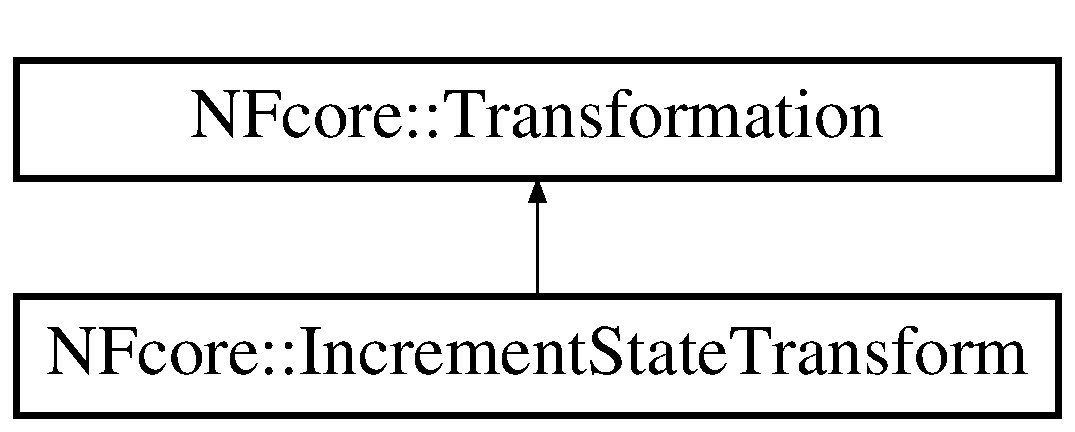
\includegraphics[height=2cm]{classNFcore_1_1IncrementStateTransform}
\end{center}
\end{figure}
\subsection*{Public Member Functions}
\begin{CompactItemize}
\item 
{\bf IncrementStateTransform} (unsigned int stateIndex)
\item 
virtual {\bf $\sim$IncrementStateTransform} ()
\item 
virtual void {\bf apply} ({\bf Mapping} $\ast$m, {\bf MappingSet} $\ast$$\ast$ms)
\item 
virtual int {\bf getComponentIndex} () const 
\end{CompactItemize}
\subsection*{Protected Attributes}
\begin{CompactItemize}
\item 
int {\bf cIndex}
\end{CompactItemize}


\subsection{Constructor \& Destructor Documentation}
\index{NFcore::IncrementStateTransform@{NFcore::IncrementStateTransform}!IncrementStateTransform@{IncrementStateTransform}}
\index{IncrementStateTransform@{IncrementStateTransform}!NFcore::IncrementStateTransform@{NFcore::IncrementStateTransform}}
\subsubsection{\setlength{\rightskip}{0pt plus 5cm}IncrementStateTransform::IncrementStateTransform (unsigned int {\em stateIndex})}\label{classNFcore_1_1IncrementStateTransform_8dc414fd7cc24cec4d97bd605b48e85f}


\index{NFcore::IncrementStateTransform@{NFcore::IncrementStateTransform}!$\sim$IncrementStateTransform@{$\sim$IncrementStateTransform}}
\index{$\sim$IncrementStateTransform@{$\sim$IncrementStateTransform}!NFcore::IncrementStateTransform@{NFcore::IncrementStateTransform}}
\subsubsection{\setlength{\rightskip}{0pt plus 5cm}virtual NFcore::IncrementStateTransform::$\sim$IncrementStateTransform ()\hspace{0.3cm}{\tt  [inline, virtual]}}\label{classNFcore_1_1IncrementStateTransform_c18e6a6e4cfd8249c920be62b1371a3f}




\subsection{Member Function Documentation}
\index{NFcore::IncrementStateTransform@{NFcore::IncrementStateTransform}!apply@{apply}}
\index{apply@{apply}!NFcore::IncrementStateTransform@{NFcore::IncrementStateTransform}}
\subsubsection{\setlength{\rightskip}{0pt plus 5cm}void IncrementStateTransform::apply ({\bf Mapping} $\ast$ {\em m}, {\bf MappingSet} $\ast$$\ast$ {\em ms})\hspace{0.3cm}{\tt  [virtual]}}\label{classNFcore_1_1IncrementStateTransform_47ec72e990cfad2110e251b2749e6a34}




Implements {\bf NFcore::Transformation} \doxyref{}{p.}{classNFcore_1_1Transformation_6a57f607676c92b2465427e57bc7fae5}.\index{NFcore::IncrementStateTransform@{NFcore::IncrementStateTransform}!getComponentIndex@{getComponentIndex}}
\index{getComponentIndex@{getComponentIndex}!NFcore::IncrementStateTransform@{NFcore::IncrementStateTransform}}
\subsubsection{\setlength{\rightskip}{0pt plus 5cm}virtual int NFcore::IncrementStateTransform::getComponentIndex () const\hspace{0.3cm}{\tt  [inline, virtual]}}\label{classNFcore_1_1IncrementStateTransform_c43495e0e7ad7ef79ad7bd8dfb940825}




Implements {\bf NFcore::Transformation} \doxyref{}{p.}{classNFcore_1_1Transformation_2ba394b20768b21ba328431103474607}.

\subsection{Member Data Documentation}
\index{NFcore::IncrementStateTransform@{NFcore::IncrementStateTransform}!cIndex@{cIndex}}
\index{cIndex@{cIndex}!NFcore::IncrementStateTransform@{NFcore::IncrementStateTransform}}
\subsubsection{\setlength{\rightskip}{0pt plus 5cm}int {\bf NFcore::IncrementStateTransform::cIndex}\hspace{0.3cm}{\tt  [protected]}}\label{classNFcore_1_1IncrementStateTransform_d2ec6b78992a4ff5a8a3f3c237f80288}




The documentation for this class was generated from the following files:\begin{CompactItemize}
\item 
/home/msneddon/eclipse/ganymede\_\-cpp/workspace/NFsim\_\-svn/src/NFreactions/transformations/{\bf transformation.hh}\item 
/home/msneddon/eclipse/ganymede\_\-cpp/workspace/NFsim\_\-svn/src/NFreactions/transformations/{\bf transformation.cpp}\end{CompactItemize}

\section{IsInWrongComplex Class Reference}
\label{classIsInWrongComplex}\index{IsInWrongComplex@{IsInWrongComplex}}
\subsection*{Public Member Functions}
\begin{CompactItemize}
\item 
{\bf IsInWrongComplex} (int currentComplexID)
\item 
bool {\bf operator()} ({\bf Molecule} $\ast$m) const 
\end{CompactItemize}


\subsection{Constructor \& Destructor Documentation}
\index{IsInWrongComplex@{IsInWrongComplex}!IsInWrongComplex@{IsInWrongComplex}}
\index{IsInWrongComplex@{IsInWrongComplex}!IsInWrongComplex@{IsInWrongComplex}}
\subsubsection{\setlength{\rightskip}{0pt plus 5cm}IsInWrongComplex::IsInWrongComplex (int {\em currentComplexID})\hspace{0.3cm}{\tt  [inline]}}\label{classIsInWrongComplex_8ffb7d3c8b148441f1ec3b4bd23362af}




\subsection{Member Function Documentation}
\index{IsInWrongComplex@{IsInWrongComplex}!operator()@{operator()}}
\index{operator()@{operator()}!IsInWrongComplex@{IsInWrongComplex}}
\subsubsection{\setlength{\rightskip}{0pt plus 5cm}bool IsInWrongComplex::operator() ({\bf Molecule} $\ast$ {\em m}) const\hspace{0.3cm}{\tt  [inline]}}\label{classIsInWrongComplex_38f0096d82bcfc84bb3b1290fcd6241a}




The documentation for this class was generated from the following file:\begin{CompactItemize}
\item 
/home/msneddon/eclipse/indigo/workspace/NFsim/src/NFcore/{\bf complex.cpp}\end{CompactItemize}

\section{NFcore::LocalFunction Class Reference}
\label{classNFcore_1_1LocalFunction}\index{NFcore::LocalFunction@{NFcore::LocalFunction}}
{\tt \#include $<$NFfunction.hh$>$}

\subsection*{Public Member Functions}
\begin{CompactItemize}
\item 
{\bf LocalFunction} ({\bf System} $\ast$s, string {\bf name}, string {\bf originalExpression}, string {\bf parsedExpression}, vector$<$ string $>$ \&args, vector$<$ string $>$ \&{\bf varRefNames}, vector$<$ string $>$ \&{\bf varObservableNames}, vector$<$ {\bf Observable} $\ast$ $>$ \&varObservables, vector$<$ int $>$ \&{\bf varRefScope}, vector$<$ string $>$ {\bf paramNames})
\item 
{\bf $\sim$LocalFunction} ()
\item 
string {\bf getName} () const 
\item 
string {\bf getNiceName} () const 
\item 
string {\bf getExpression} () const 
\item 
string {\bf getParsedExpression} () const 
\item 
void {\bf printDetails} ({\bf System} $\ast$s)
\item 
void {\bf prepareForSimulation} ({\bf System} $\ast$s)
\item 
double {\bf getValue} ({\bf Molecule} $\ast$m, int scope)
\item 
double {\bf evaluateOn} ({\bf Molecule} $\ast$m, int scope)
\item 
void {\bf addTypeIMoleculeDependency} ({\bf MoleculeType} $\ast$mt)
\item 
void {\bf updateParameters} ({\bf System} $\ast$s)
\end{CompactItemize}
\subsection*{Public Attributes}
\begin{CompactItemize}
\item 
mu::Parser $\ast$ {\bf p}
\end{CompactItemize}
\subsection*{Static Public Attributes}
\begin{CompactItemize}
\item 
static const int {\bf SPECIES} = 0
\item 
static const int {\bf MOLECULE} = 1
\end{CompactItemize}
\subsection*{Protected Attributes}
\begin{CompactItemize}
\item 
string {\bf name}
\item 
string {\bf nicename}
\item 
string {\bf originalExpression}
\item 
string {\bf parsedExpression}
\item 
unsigned int {\bf n\_\-args}
\item 
string $\ast$ {\bf argNames}
\item 
unsigned int {\bf n\_\-params}
\item 
string $\ast$ {\bf paramNames}
\item 
unsigned int {\bf n\_\-varRefs}
\item 
string $\ast$ {\bf varRefNames}
\item 
string $\ast$ {\bf varObservableNames}
\item 
int $\ast$ {\bf varRefScope}
\item 
{\bf Observable} $\ast$$\ast$ {\bf varLocalObservables}
\item 
vector$<$ {\bf MoleculeType} $\ast$ $>$ {\bf typeI\_\-mol}
\item 
vector$<$ int $>$ {\bf typeI\_\-localFunctionIndex}
\item 
int {\bf n\_\-typeIImolecules}
\item 
{\bf MoleculeType} $\ast$$\ast$ {\bf typeII\_\-mol}
\item 
vector$<$ int $>$ {\bf typeII\_\-localFunctionIndex}
\end{CompactItemize}
\subsection*{Static Protected Attributes}
\begin{CompactItemize}
\item 
static list$<$ {\bf Molecule} $\ast$ $>$ {\bf molList}
\item 
static list$<$ {\bf Molecule} $\ast$ $>$::iterator {\bf molIter}
\end{CompactItemize}


\subsection{Constructor \& Destructor Documentation}
\index{NFcore::LocalFunction@{NFcore::LocalFunction}!LocalFunction@{LocalFunction}}
\index{LocalFunction@{LocalFunction}!NFcore::LocalFunction@{NFcore::LocalFunction}}
\subsubsection{\setlength{\rightskip}{0pt plus 5cm}LocalFunction::LocalFunction ({\bf System} $\ast$ {\em s}, string {\em name}, string {\em originalExpression}, string {\em parsedExpression}, vector$<$ string $>$ \& {\em args}, vector$<$ string $>$ \& {\em varRefNames}, vector$<$ string $>$ \& {\em varObservableNames}, vector$<$ {\bf Observable} $\ast$ $>$ \& {\em varObservables}, vector$<$ int $>$ \& {\em varRefScope}, vector$<$ string $>$ {\em paramNames})}\label{classNFcore_1_1LocalFunction_7c669519fe3ec402f65c8117372da775}


\index{NFcore::LocalFunction@{NFcore::LocalFunction}!$\sim$LocalFunction@{$\sim$LocalFunction}}
\index{$\sim$LocalFunction@{$\sim$LocalFunction}!NFcore::LocalFunction@{NFcore::LocalFunction}}
\subsubsection{\setlength{\rightskip}{0pt plus 5cm}LocalFunction::$\sim$LocalFunction ()}\label{classNFcore_1_1LocalFunction_a78ebddc2c447014891ac0b591e39445}




\subsection{Member Function Documentation}
\index{NFcore::LocalFunction@{NFcore::LocalFunction}!getName@{getName}}
\index{getName@{getName}!NFcore::LocalFunction@{NFcore::LocalFunction}}
\subsubsection{\setlength{\rightskip}{0pt plus 5cm}string LocalFunction::getName () const}\label{classNFcore_1_1LocalFunction_53e067c7b8d204ab4c8cf552b000999d}


\index{NFcore::LocalFunction@{NFcore::LocalFunction}!getNiceName@{getNiceName}}
\index{getNiceName@{getNiceName}!NFcore::LocalFunction@{NFcore::LocalFunction}}
\subsubsection{\setlength{\rightskip}{0pt plus 5cm}string LocalFunction::getNiceName () const}\label{classNFcore_1_1LocalFunction_ccb96efc45b9c37eb77b86389877a9ed}


\index{NFcore::LocalFunction@{NFcore::LocalFunction}!getExpression@{getExpression}}
\index{getExpression@{getExpression}!NFcore::LocalFunction@{NFcore::LocalFunction}}
\subsubsection{\setlength{\rightskip}{0pt plus 5cm}string LocalFunction::getExpression () const}\label{classNFcore_1_1LocalFunction_34e2e490a88cefddafd4ca05459779f0}


\index{NFcore::LocalFunction@{NFcore::LocalFunction}!getParsedExpression@{getParsedExpression}}
\index{getParsedExpression@{getParsedExpression}!NFcore::LocalFunction@{NFcore::LocalFunction}}
\subsubsection{\setlength{\rightskip}{0pt plus 5cm}string LocalFunction::getParsedExpression () const}\label{classNFcore_1_1LocalFunction_280382a148d8cf1adde257faaa3f8ab3}


\index{NFcore::LocalFunction@{NFcore::LocalFunction}!printDetails@{printDetails}}
\index{printDetails@{printDetails}!NFcore::LocalFunction@{NFcore::LocalFunction}}
\subsubsection{\setlength{\rightskip}{0pt plus 5cm}void LocalFunction::printDetails ({\bf System} $\ast$ {\em s})}\label{classNFcore_1_1LocalFunction_20531f336920310a7827841df3e3e60a}


\index{NFcore::LocalFunction@{NFcore::LocalFunction}!prepareForSimulation@{prepareForSimulation}}
\index{prepareForSimulation@{prepareForSimulation}!NFcore::LocalFunction@{NFcore::LocalFunction}}
\subsubsection{\setlength{\rightskip}{0pt plus 5cm}void LocalFunction::prepareForSimulation ({\bf System} $\ast$ {\em s})}\label{classNFcore_1_1LocalFunction_78194708521f4f38d9167a729d6faaaf}


\index{NFcore::LocalFunction@{NFcore::LocalFunction}!getValue@{getValue}}
\index{getValue@{getValue}!NFcore::LocalFunction@{NFcore::LocalFunction}}
\subsubsection{\setlength{\rightskip}{0pt plus 5cm}double LocalFunction::getValue ({\bf Molecule} $\ast$ {\em m}, int {\em scope})}\label{classNFcore_1_1LocalFunction_216854e02c151f6d0d9cf61ea63c6eb2}


\index{NFcore::LocalFunction@{NFcore::LocalFunction}!evaluateOn@{evaluateOn}}
\index{evaluateOn@{evaluateOn}!NFcore::LocalFunction@{NFcore::LocalFunction}}
\subsubsection{\setlength{\rightskip}{0pt plus 5cm}double LocalFunction::evaluateOn ({\bf Molecule} $\ast$ {\em m}, int {\em scope})}\label{classNFcore_1_1LocalFunction_d2dd436e78f735368db406747556bcd7}


\index{NFcore::LocalFunction@{NFcore::LocalFunction}!addTypeIMoleculeDependency@{addTypeIMoleculeDependency}}
\index{addTypeIMoleculeDependency@{addTypeIMoleculeDependency}!NFcore::LocalFunction@{NFcore::LocalFunction}}
\subsubsection{\setlength{\rightskip}{0pt plus 5cm}void LocalFunction::addTypeIMoleculeDependency ({\bf MoleculeType} $\ast$ {\em mt})}\label{classNFcore_1_1LocalFunction_106c3395c67c310f720e904e36ab0fe2}


\index{NFcore::LocalFunction@{NFcore::LocalFunction}!updateParameters@{updateParameters}}
\index{updateParameters@{updateParameters}!NFcore::LocalFunction@{NFcore::LocalFunction}}
\subsubsection{\setlength{\rightskip}{0pt plus 5cm}void LocalFunction::updateParameters ({\bf System} $\ast$ {\em s})}\label{classNFcore_1_1LocalFunction_66d11851be45bdb8dd91b39670c8a3f7}




\subsection{Member Data Documentation}
\index{NFcore::LocalFunction@{NFcore::LocalFunction}!SPECIES@{SPECIES}}
\index{SPECIES@{SPECIES}!NFcore::LocalFunction@{NFcore::LocalFunction}}
\subsubsection{\setlength{\rightskip}{0pt plus 5cm}const int {\bf NFcore::LocalFunction::SPECIES} = 0\hspace{0.3cm}{\tt  [static]}}\label{classNFcore_1_1LocalFunction_631b9459359729d43d3520568dfaf9b9}


\index{NFcore::LocalFunction@{NFcore::LocalFunction}!MOLECULE@{MOLECULE}}
\index{MOLECULE@{MOLECULE}!NFcore::LocalFunction@{NFcore::LocalFunction}}
\subsubsection{\setlength{\rightskip}{0pt plus 5cm}const int {\bf NFcore::LocalFunction::MOLECULE} = 1\hspace{0.3cm}{\tt  [static]}}\label{classNFcore_1_1LocalFunction_75212d20f5301281a93b87deb6a43377}


\index{NFcore::LocalFunction@{NFcore::LocalFunction}!p@{p}}
\index{p@{p}!NFcore::LocalFunction@{NFcore::LocalFunction}}
\subsubsection{\setlength{\rightskip}{0pt plus 5cm}mu::Parser$\ast$ {\bf NFcore::LocalFunction::p}}\label{classNFcore_1_1LocalFunction_357eb0be17fca1e7cecf1889c77e09ab}


\index{NFcore::LocalFunction@{NFcore::LocalFunction}!name@{name}}
\index{name@{name}!NFcore::LocalFunction@{NFcore::LocalFunction}}
\subsubsection{\setlength{\rightskip}{0pt plus 5cm}string {\bf NFcore::LocalFunction::name}\hspace{0.3cm}{\tt  [protected]}}\label{classNFcore_1_1LocalFunction_180d78e57b560f518601ea00abe93cc1}


\index{NFcore::LocalFunction@{NFcore::LocalFunction}!nicename@{nicename}}
\index{nicename@{nicename}!NFcore::LocalFunction@{NFcore::LocalFunction}}
\subsubsection{\setlength{\rightskip}{0pt plus 5cm}string {\bf NFcore::LocalFunction::nicename}\hspace{0.3cm}{\tt  [protected]}}\label{classNFcore_1_1LocalFunction_fd440817c06cfd32fbedb92a624a7d8c}


\index{NFcore::LocalFunction@{NFcore::LocalFunction}!originalExpression@{originalExpression}}
\index{originalExpression@{originalExpression}!NFcore::LocalFunction@{NFcore::LocalFunction}}
\subsubsection{\setlength{\rightskip}{0pt plus 5cm}string {\bf NFcore::LocalFunction::originalExpression}\hspace{0.3cm}{\tt  [protected]}}\label{classNFcore_1_1LocalFunction_575bcbed465855ba7ab45e87c17c47a8}


\index{NFcore::LocalFunction@{NFcore::LocalFunction}!parsedExpression@{parsedExpression}}
\index{parsedExpression@{parsedExpression}!NFcore::LocalFunction@{NFcore::LocalFunction}}
\subsubsection{\setlength{\rightskip}{0pt plus 5cm}string {\bf NFcore::LocalFunction::parsedExpression}\hspace{0.3cm}{\tt  [protected]}}\label{classNFcore_1_1LocalFunction_4572b6b4acff5c3930e9b86941d69969}


\index{NFcore::LocalFunction@{NFcore::LocalFunction}!n\_\-args@{n\_\-args}}
\index{n\_\-args@{n\_\-args}!NFcore::LocalFunction@{NFcore::LocalFunction}}
\subsubsection{\setlength{\rightskip}{0pt plus 5cm}unsigned int {\bf NFcore::LocalFunction::n\_\-args}\hspace{0.3cm}{\tt  [protected]}}\label{classNFcore_1_1LocalFunction_78a13bca5c8d724f126862b8d09392f4}


\index{NFcore::LocalFunction@{NFcore::LocalFunction}!argNames@{argNames}}
\index{argNames@{argNames}!NFcore::LocalFunction@{NFcore::LocalFunction}}
\subsubsection{\setlength{\rightskip}{0pt plus 5cm}string$\ast$ {\bf NFcore::LocalFunction::argNames}\hspace{0.3cm}{\tt  [protected]}}\label{classNFcore_1_1LocalFunction_7ab8c060b1b626e539606b1695e516b2}


\index{NFcore::LocalFunction@{NFcore::LocalFunction}!n\_\-params@{n\_\-params}}
\index{n\_\-params@{n\_\-params}!NFcore::LocalFunction@{NFcore::LocalFunction}}
\subsubsection{\setlength{\rightskip}{0pt plus 5cm}unsigned int {\bf NFcore::LocalFunction::n\_\-params}\hspace{0.3cm}{\tt  [protected]}}\label{classNFcore_1_1LocalFunction_2af28cf4caaa2d8437f9021a88b46c15}


\index{NFcore::LocalFunction@{NFcore::LocalFunction}!paramNames@{paramNames}}
\index{paramNames@{paramNames}!NFcore::LocalFunction@{NFcore::LocalFunction}}
\subsubsection{\setlength{\rightskip}{0pt plus 5cm}string$\ast$ {\bf NFcore::LocalFunction::paramNames}\hspace{0.3cm}{\tt  [protected]}}\label{classNFcore_1_1LocalFunction_33700bd74d5284c805b03628d255388f}


\index{NFcore::LocalFunction@{NFcore::LocalFunction}!n\_\-varRefs@{n\_\-varRefs}}
\index{n\_\-varRefs@{n\_\-varRefs}!NFcore::LocalFunction@{NFcore::LocalFunction}}
\subsubsection{\setlength{\rightskip}{0pt plus 5cm}unsigned int {\bf NFcore::LocalFunction::n\_\-varRefs}\hspace{0.3cm}{\tt  [protected]}}\label{classNFcore_1_1LocalFunction_d21b0b0d54df4613e24619a4779d0326}


\index{NFcore::LocalFunction@{NFcore::LocalFunction}!varRefNames@{varRefNames}}
\index{varRefNames@{varRefNames}!NFcore::LocalFunction@{NFcore::LocalFunction}}
\subsubsection{\setlength{\rightskip}{0pt plus 5cm}string$\ast$ {\bf NFcore::LocalFunction::varRefNames}\hspace{0.3cm}{\tt  [protected]}}\label{classNFcore_1_1LocalFunction_dc858f57c65c66538d087f80485f456c}


\index{NFcore::LocalFunction@{NFcore::LocalFunction}!varObservableNames@{varObservableNames}}
\index{varObservableNames@{varObservableNames}!NFcore::LocalFunction@{NFcore::LocalFunction}}
\subsubsection{\setlength{\rightskip}{0pt plus 5cm}string$\ast$ {\bf NFcore::LocalFunction::varObservableNames}\hspace{0.3cm}{\tt  [protected]}}\label{classNFcore_1_1LocalFunction_5e70ae1a4e2b50324c8c035a06055fc7}


\index{NFcore::LocalFunction@{NFcore::LocalFunction}!varRefScope@{varRefScope}}
\index{varRefScope@{varRefScope}!NFcore::LocalFunction@{NFcore::LocalFunction}}
\subsubsection{\setlength{\rightskip}{0pt plus 5cm}int$\ast$ {\bf NFcore::LocalFunction::varRefScope}\hspace{0.3cm}{\tt  [protected]}}\label{classNFcore_1_1LocalFunction_2d28e00727b049acd315a26c08c00b3f}


\index{NFcore::LocalFunction@{NFcore::LocalFunction}!varLocalObservables@{varLocalObservables}}
\index{varLocalObservables@{varLocalObservables}!NFcore::LocalFunction@{NFcore::LocalFunction}}
\subsubsection{\setlength{\rightskip}{0pt plus 5cm}{\bf Observable}$\ast$$\ast$ {\bf NFcore::LocalFunction::varLocalObservables}\hspace{0.3cm}{\tt  [protected]}}\label{classNFcore_1_1LocalFunction_c323425b06d5f6d354ba2f6f88f49a9d}


\index{NFcore::LocalFunction@{NFcore::LocalFunction}!molList@{molList}}
\index{molList@{molList}!NFcore::LocalFunction@{NFcore::LocalFunction}}
\subsubsection{\setlength{\rightskip}{0pt plus 5cm}list$<$ {\bf Molecule} $\ast$ $>$ {\bf LocalFunction::molList}\hspace{0.3cm}{\tt  [static, protected]}}\label{classNFcore_1_1LocalFunction_9eb147b90ff439b16a009f737bf8af60}


\index{NFcore::LocalFunction@{NFcore::LocalFunction}!molIter@{molIter}}
\index{molIter@{molIter}!NFcore::LocalFunction@{NFcore::LocalFunction}}
\subsubsection{\setlength{\rightskip}{0pt plus 5cm}list$<$ {\bf Molecule} $\ast$ $>$::iterator {\bf LocalFunction::molIter}\hspace{0.3cm}{\tt  [static, protected]}}\label{classNFcore_1_1LocalFunction_695d9899671a07a84e567f592011be62}


\index{NFcore::LocalFunction@{NFcore::LocalFunction}!typeI\_\-mol@{typeI\_\-mol}}
\index{typeI\_\-mol@{typeI\_\-mol}!NFcore::LocalFunction@{NFcore::LocalFunction}}
\subsubsection{\setlength{\rightskip}{0pt plus 5cm}vector$<${\bf MoleculeType} $\ast$$>$ {\bf NFcore::LocalFunction::typeI\_\-mol}\hspace{0.3cm}{\tt  [protected]}}\label{classNFcore_1_1LocalFunction_37e3bd04f3b6e7c1fe99c66459f8aeb5}


\index{NFcore::LocalFunction@{NFcore::LocalFunction}!typeI\_\-localFunctionIndex@{typeI\_\-localFunctionIndex}}
\index{typeI\_\-localFunctionIndex@{typeI\_\-localFunctionIndex}!NFcore::LocalFunction@{NFcore::LocalFunction}}
\subsubsection{\setlength{\rightskip}{0pt plus 5cm}vector$<$int$>$ {\bf NFcore::LocalFunction::typeI\_\-localFunctionIndex}\hspace{0.3cm}{\tt  [protected]}}\label{classNFcore_1_1LocalFunction_c91487d90e85032a532af09eac26bb15}


\index{NFcore::LocalFunction@{NFcore::LocalFunction}!n\_\-typeIImolecules@{n\_\-typeIImolecules}}
\index{n\_\-typeIImolecules@{n\_\-typeIImolecules}!NFcore::LocalFunction@{NFcore::LocalFunction}}
\subsubsection{\setlength{\rightskip}{0pt plus 5cm}int {\bf NFcore::LocalFunction::n\_\-typeIImolecules}\hspace{0.3cm}{\tt  [protected]}}\label{classNFcore_1_1LocalFunction_02acb589165bf598387771403bd78e04}


\index{NFcore::LocalFunction@{NFcore::LocalFunction}!typeII\_\-mol@{typeII\_\-mol}}
\index{typeII\_\-mol@{typeII\_\-mol}!NFcore::LocalFunction@{NFcore::LocalFunction}}
\subsubsection{\setlength{\rightskip}{0pt plus 5cm}{\bf MoleculeType}$\ast$$\ast$ {\bf NFcore::LocalFunction::typeII\_\-mol}\hspace{0.3cm}{\tt  [protected]}}\label{classNFcore_1_1LocalFunction_18a40f1cc4dba13502a542c60aa3961d}


\index{NFcore::LocalFunction@{NFcore::LocalFunction}!typeII\_\-localFunctionIndex@{typeII\_\-localFunctionIndex}}
\index{typeII\_\-localFunctionIndex@{typeII\_\-localFunctionIndex}!NFcore::LocalFunction@{NFcore::LocalFunction}}
\subsubsection{\setlength{\rightskip}{0pt plus 5cm}vector$<$int$>$ {\bf NFcore::LocalFunction::typeII\_\-localFunctionIndex}\hspace{0.3cm}{\tt  [protected]}}\label{classNFcore_1_1LocalFunction_90a0774ef85096dbdd99ccabcc045553}




The documentation for this class was generated from the following files:\begin{CompactItemize}
\item 
/home/msneddon/eclipse/galileoSR1\_\-cpp/workspace/NFsim/src/NFfunction/{\bf NFfunction.hh}\item 
/home/msneddon/eclipse/galileoSR1\_\-cpp/workspace/NFsim/src/NFfunction/{\bf localFunction.cpp}\end{CompactItemize}

\section{NFcore::LocalFunctionReference Class Reference}
\label{classNFcore_1_1LocalFunctionReference}\index{NFcore::LocalFunctionReference@{NFcore::LocalFunctionReference}}
{\tt \#include $<$transformation.hh$>$}

Inheritance diagram for NFcore::LocalFunctionReference::\begin{figure}[H]
\begin{center}
\leavevmode
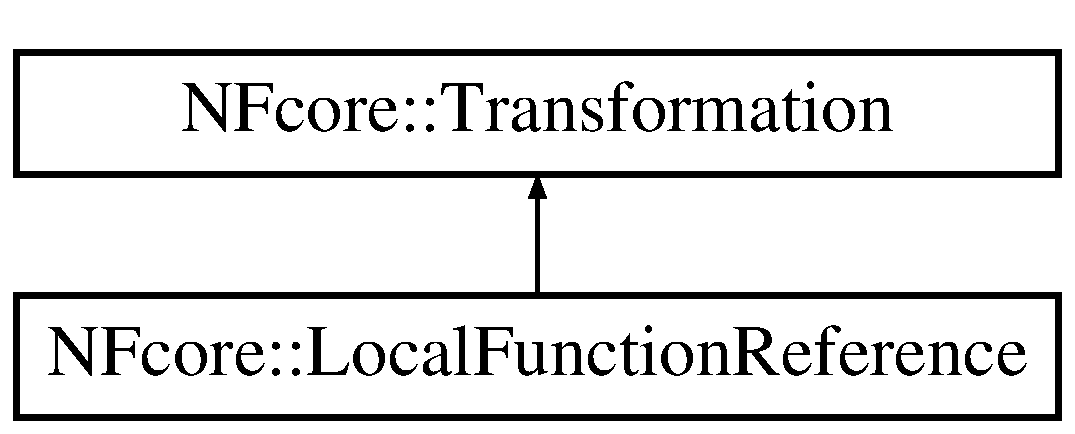
\includegraphics[height=2cm]{classNFcore_1_1LocalFunctionReference}
\end{center}
\end{figure}
\subsection*{Public Member Functions}
\begin{CompactItemize}
\item 
{\bf LocalFunctionReference} (string {\bf PointerName}, int {\bf scope}, {\bf TemplateMolecule} $\ast${\bf tm})
\item 
virtual {\bf $\sim$LocalFunctionReference} ()
\item 
virtual void {\bf apply} ({\bf Mapping} $\ast$m, {\bf MappingSet} $\ast$$\ast$ms)
\item 
virtual int {\bf getComponentIndex} () const 
\item 
{\bf TemplateMolecule} $\ast$ {\bf getTemplateObject} () const 
\item 
string {\bf getPointerName} () const 
\item 
int {\bf getFunctionScope} () const 
\end{CompactItemize}
\subsection*{Static Public Attributes}
\begin{CompactItemize}
\item 
static const unsigned int {\bf SPECIES\_\-FUNCTION} = 0
\item 
static const unsigned int {\bf SINGLE\_\-MOLECULE\_\-FUNCTION} = 1
\end{CompactItemize}
\subsection*{Protected Attributes}
\begin{CompactItemize}
\item 
string {\bf PointerName}
\item 
int {\bf scope}
\item 
{\bf TemplateMolecule} $\ast$ {\bf tm}
\end{CompactItemize}


\subsection{Constructor \& Destructor Documentation}
\index{NFcore::LocalFunctionReference@{NFcore::LocalFunctionReference}!LocalFunctionReference@{LocalFunctionReference}}
\index{LocalFunctionReference@{LocalFunctionReference}!NFcore::LocalFunctionReference@{NFcore::LocalFunctionReference}}
\subsubsection{\setlength{\rightskip}{0pt plus 5cm}LocalFunctionReference::LocalFunctionReference (string {\em PointerName}, int {\em scope}, {\bf TemplateMolecule} $\ast$ {\em tm})}\label{classNFcore_1_1LocalFunctionReference_1731ea3deb7948a39637d63eef5945f1}


\index{NFcore::LocalFunctionReference@{NFcore::LocalFunctionReference}!$\sim$LocalFunctionReference@{$\sim$LocalFunctionReference}}
\index{$\sim$LocalFunctionReference@{$\sim$LocalFunctionReference}!NFcore::LocalFunctionReference@{NFcore::LocalFunctionReference}}
\subsubsection{\setlength{\rightskip}{0pt plus 5cm}virtual NFcore::LocalFunctionReference::$\sim$LocalFunctionReference ()\hspace{0.3cm}{\tt  [inline, virtual]}}\label{classNFcore_1_1LocalFunctionReference_11e483457f93eeddfc988ec6b6f99f09}




\subsection{Member Function Documentation}
\index{NFcore::LocalFunctionReference@{NFcore::LocalFunctionReference}!apply@{apply}}
\index{apply@{apply}!NFcore::LocalFunctionReference@{NFcore::LocalFunctionReference}}
\subsubsection{\setlength{\rightskip}{0pt plus 5cm}virtual void NFcore::LocalFunctionReference::apply ({\bf Mapping} $\ast$ {\em m}, {\bf MappingSet} $\ast$$\ast$ {\em ms})\hspace{0.3cm}{\tt  [inline, virtual]}}\label{classNFcore_1_1LocalFunctionReference_62280a5922e15fcda20b801ca2662ba8}




Implements {\bf NFcore::Transformation} \doxyref{}{p.}{classNFcore_1_1Transformation_6a57f607676c92b2465427e57bc7fae5}.\index{NFcore::LocalFunctionReference@{NFcore::LocalFunctionReference}!getComponentIndex@{getComponentIndex}}
\index{getComponentIndex@{getComponentIndex}!NFcore::LocalFunctionReference@{NFcore::LocalFunctionReference}}
\subsubsection{\setlength{\rightskip}{0pt plus 5cm}virtual int NFcore::LocalFunctionReference::getComponentIndex () const\hspace{0.3cm}{\tt  [inline, virtual]}}\label{classNFcore_1_1LocalFunctionReference_fad70297f131516af5b68ef5f508dfc9}




Implements {\bf NFcore::Transformation} \doxyref{}{p.}{classNFcore_1_1Transformation_2ba394b20768b21ba328431103474607}.\index{NFcore::LocalFunctionReference@{NFcore::LocalFunctionReference}!getTemplateObject@{getTemplateObject}}
\index{getTemplateObject@{getTemplateObject}!NFcore::LocalFunctionReference@{NFcore::LocalFunctionReference}}
\subsubsection{\setlength{\rightskip}{0pt plus 5cm}{\bf TemplateMolecule}$\ast$ NFcore::LocalFunctionReference::getTemplateObject () const\hspace{0.3cm}{\tt  [inline]}}\label{classNFcore_1_1LocalFunctionReference_2cae2fb1d9e93fffdf19cad90d5179de}


\index{NFcore::LocalFunctionReference@{NFcore::LocalFunctionReference}!getPointerName@{getPointerName}}
\index{getPointerName@{getPointerName}!NFcore::LocalFunctionReference@{NFcore::LocalFunctionReference}}
\subsubsection{\setlength{\rightskip}{0pt plus 5cm}string NFcore::LocalFunctionReference::getPointerName () const\hspace{0.3cm}{\tt  [inline]}}\label{classNFcore_1_1LocalFunctionReference_678751a7f9100b013311ee46f1f71219}


\index{NFcore::LocalFunctionReference@{NFcore::LocalFunctionReference}!getFunctionScope@{getFunctionScope}}
\index{getFunctionScope@{getFunctionScope}!NFcore::LocalFunctionReference@{NFcore::LocalFunctionReference}}
\subsubsection{\setlength{\rightskip}{0pt plus 5cm}int NFcore::LocalFunctionReference::getFunctionScope () const\hspace{0.3cm}{\tt  [inline]}}\label{classNFcore_1_1LocalFunctionReference_d043390c7a517b67f8ba93e25549c991}




\subsection{Member Data Documentation}
\index{NFcore::LocalFunctionReference@{NFcore::LocalFunctionReference}!SPECIES\_\-FUNCTION@{SPECIES\_\-FUNCTION}}
\index{SPECIES\_\-FUNCTION@{SPECIES\_\-FUNCTION}!NFcore::LocalFunctionReference@{NFcore::LocalFunctionReference}}
\subsubsection{\setlength{\rightskip}{0pt plus 5cm}const unsigned int {\bf NFcore::LocalFunctionReference::SPECIES\_\-FUNCTION} = 0\hspace{0.3cm}{\tt  [static]}}\label{classNFcore_1_1LocalFunctionReference_893b69db1604da6aa694acd9adf824d2}


\index{NFcore::LocalFunctionReference@{NFcore::LocalFunctionReference}!SINGLE\_\-MOLECULE\_\-FUNCTION@{SINGLE\_\-MOLECULE\_\-FUNCTION}}
\index{SINGLE\_\-MOLECULE\_\-FUNCTION@{SINGLE\_\-MOLECULE\_\-FUNCTION}!NFcore::LocalFunctionReference@{NFcore::LocalFunctionReference}}
\subsubsection{\setlength{\rightskip}{0pt plus 5cm}const unsigned int {\bf NFcore::LocalFunctionReference::SINGLE\_\-MOLECULE\_\-FUNCTION} = 1\hspace{0.3cm}{\tt  [static]}}\label{classNFcore_1_1LocalFunctionReference_c44f27d48b64f9c9c412970ade46a711}


\index{NFcore::LocalFunctionReference@{NFcore::LocalFunctionReference}!PointerName@{PointerName}}
\index{PointerName@{PointerName}!NFcore::LocalFunctionReference@{NFcore::LocalFunctionReference}}
\subsubsection{\setlength{\rightskip}{0pt plus 5cm}string {\bf NFcore::LocalFunctionReference::PointerName}\hspace{0.3cm}{\tt  [protected]}}\label{classNFcore_1_1LocalFunctionReference_bce12cc1cb508bd514a6d080ca586532}


\index{NFcore::LocalFunctionReference@{NFcore::LocalFunctionReference}!scope@{scope}}
\index{scope@{scope}!NFcore::LocalFunctionReference@{NFcore::LocalFunctionReference}}
\subsubsection{\setlength{\rightskip}{0pt plus 5cm}int {\bf NFcore::LocalFunctionReference::scope}\hspace{0.3cm}{\tt  [protected]}}\label{classNFcore_1_1LocalFunctionReference_5fcaa44549aff151b12b23f5aaa4871b}


\index{NFcore::LocalFunctionReference@{NFcore::LocalFunctionReference}!tm@{tm}}
\index{tm@{tm}!NFcore::LocalFunctionReference@{NFcore::LocalFunctionReference}}
\subsubsection{\setlength{\rightskip}{0pt plus 5cm}{\bf TemplateMolecule}$\ast$ {\bf NFcore::LocalFunctionReference::tm}\hspace{0.3cm}{\tt  [protected]}}\label{classNFcore_1_1LocalFunctionReference_8472d7bb34ad1fbef670aa528000746e}




The documentation for this class was generated from the following files:\begin{CompactItemize}
\item 
/home/msneddon/eclipse/galileoSR1\_\-cpp/workspace/NFsim/src/NFreactions/transformations/{\bf transformation.hh}\item 
/home/msneddon/eclipse/galileoSR1\_\-cpp/workspace/NFsim/src/NFreactions/transformations/{\bf transformation.cpp}\end{CompactItemize}

\section{NFcore::MapGenerator Class Reference}
\label{classNFcore_1_1MapGenerator}\index{NFcore::MapGenerator@{NFcore::MapGenerator}}
{\tt \#include $<$mappingGenerator.hh$>$}



\subsection{Detailed Description}
Knows how to assign mappings in a \doxyref{MappingSet}{p.}{classNFcore_1_1MappingSet} to a particular \doxyref{Molecule}{p.}{classNFcore_1_1Molecule}. 

MapGenerators are simple objects given to TemplateMolecules (so are maintained and deleted by \doxyref{TemplateMolecule}{p.}{classNFcore_1_1TemplateMolecule} objects) that assign \doxyref{Mapping}{p.}{classNFcore_1_1Mapping} objects to particular \doxyref{Molecule}{p.}{classNFcore_1_1Molecule} objects. This allows us to Map specific components of a reactant as we compare the potential molecules to the \doxyref{TemplateMolecule}{p.}{classNFcore_1_1TemplateMolecule}. (see the \doxyref{TemplateMolecule}{p.}{classNFcore_1_1TemplateMolecule} compare() functions). If there is a match, the Template \doxyref{Molecule}{p.}{classNFcore_1_1Molecule} uses this to assign a mapping. This class is useful because it knows which \doxyref{Mapping}{p.}{classNFcore_1_1Mapping} to use in the \doxyref{MappingSet}{p.}{classNFcore_1_1MappingSet} provided in the \doxyref{map()}{p.}{classNFcore_1_1MapGenerator_1276176a858d99789be940a93d4b83ae} function. This is necessary information as we always reuse \doxyref{Mapping}{p.}{classNFcore_1_1Mapping} and \doxyref{MappingSet}{p.}{classNFcore_1_1MappingSet} objects for effeciency. \begin{Desc}
\item[Author:]Michael Sneddon \end{Desc}
\subsection*{Public Member Functions}
\begin{CompactItemize}
\item 
{\bf MapGenerator} (unsigned int {\bf mappingIndex})
\item 
{\bf $\sim$MapGenerator} ()
\item 
bool {\bf map} ({\bf MappingSet} $\ast$mappingSet, {\bf Molecule} $\ast$molecule)
\end{CompactItemize}
\subsection*{Protected Attributes}
\begin{CompactItemize}
\item 
unsigned int {\bf mappingIndex}
\end{CompactItemize}


\subsection{Constructor \& Destructor Documentation}
\index{NFcore::MapGenerator@{NFcore::MapGenerator}!MapGenerator@{MapGenerator}}
\index{MapGenerator@{MapGenerator}!NFcore::MapGenerator@{NFcore::MapGenerator}}
\subsubsection{\setlength{\rightskip}{0pt plus 5cm}MapGenerator::MapGenerator (unsigned int {\em mappingIndex})}\label{classNFcore_1_1MapGenerator_7cbf945f55fe6131f36390d73d445fe4}


Creates a \doxyref{MapGenerator}{p.}{classNFcore_1_1MapGenerator} (generally created in a \doxyref{TransformationSet}{p.}{classNFcore_1_1TransformationSet} when we are creating Transformations) that remembers the index of a \doxyref{Mapping}{p.}{classNFcore_1_1Mapping} in a \doxyref{MappingSet}{p.}{classNFcore_1_1MappingSet} so that we always reuse the same \doxyref{Mapping}{p.}{classNFcore_1_1Mapping}. \begin{Desc}
\item[Author:]Michael Sneddon \end{Desc}
\index{NFcore::MapGenerator@{NFcore::MapGenerator}!$\sim$MapGenerator@{$\sim$MapGenerator}}
\index{$\sim$MapGenerator@{$\sim$MapGenerator}!NFcore::MapGenerator@{NFcore::MapGenerator}}
\subsubsection{\setlength{\rightskip}{0pt plus 5cm}NFcore::MapGenerator::$\sim$MapGenerator ()\hspace{0.3cm}{\tt  [inline]}}\label{classNFcore_1_1MapGenerator_4cf1ecd3d7a23859d2620cd0959a0dfd}


Deconstructor that does nothing significant. \begin{Desc}
\item[Author:]Michael Sneddon \end{Desc}


\subsection{Member Function Documentation}
\index{NFcore::MapGenerator@{NFcore::MapGenerator}!map@{map}}
\index{map@{map}!NFcore::MapGenerator@{NFcore::MapGenerator}}
\subsubsection{\setlength{\rightskip}{0pt plus 5cm}bool MapGenerator::map ({\bf MappingSet} $\ast$ {\em mappingSet}, {\bf Molecule} $\ast$ {\em molecule})}\label{classNFcore_1_1MapGenerator_1276176a858d99789be940a93d4b83ae}


The one key function of a \doxyref{MapGenerator}{p.}{classNFcore_1_1MapGenerator} - this takes a \doxyref{MappingSet}{p.}{classNFcore_1_1MappingSet} and finds the particular \doxyref{Mapping}{p.}{classNFcore_1_1Mapping} that this \doxyref{MapGenerator}{p.}{classNFcore_1_1MapGenerator} needs to create and sets that \doxyref{Mapping}{p.}{classNFcore_1_1Mapping} to point to the given molecule. This is called in the \doxyref{TemplateMolecule}{p.}{classNFcore_1_1TemplateMolecule} compare() function. \begin{Desc}
\item[Author:]Michael Sneddon \end{Desc}


\subsection{Member Data Documentation}
\index{NFcore::MapGenerator@{NFcore::MapGenerator}!mappingIndex@{mappingIndex}}
\index{mappingIndex@{mappingIndex}!NFcore::MapGenerator@{NFcore::MapGenerator}}
\subsubsection{\setlength{\rightskip}{0pt plus 5cm}unsigned int {\bf NFcore::MapGenerator::mappingIndex}\hspace{0.3cm}{\tt  [protected]}}\label{classNFcore_1_1MapGenerator_806fe3e757d9f19b07a520689dd34877}


Keeps track of the index of the \doxyref{Mapping}{p.}{classNFcore_1_1Mapping} in the \doxyref{MappingSet}{p.}{classNFcore_1_1MappingSet} that this \doxyref{MapGenerator}{p.}{classNFcore_1_1MapGenerator} must assign. 

The documentation for this class was generated from the following files:\begin{CompactItemize}
\item 
/home/msneddon/eclipse/galileoSR1\_\-cpp/workspace/NFsim/src/NFreactions/mappings/{\bf mappingGenerator.hh}\item 
/home/msneddon/eclipse/galileoSR1\_\-cpp/workspace/NFsim/src/NFreactions/mappings/{\bf mappingGenerator.cpp}\end{CompactItemize}

\section{NFcore::Mapping Class Reference}
\label{classNFcore_1_1Mapping}\index{NFcore::Mapping@{NFcore::Mapping}}
{\tt \#include $<$mapping.hh$>$}



\subsection{Detailed Description}
Keeps a pointer to a molecule and remembers a single component to act on. 

This is the low level unit that is used by reactions to identify the particular component of a molecule to update or change when a transformation is required. It is maintained by a \doxyref{MappingSet}{p.}{classNFcore_1_1MappingSet} which is just a collection of \doxyref{Mapping}{p.}{classNFcore_1_1Mapping} objects. The \char`\"{}type\char`\"{} of mapping is identified in the same way as the \char`\"{}type\char`\"{} of transformation. See the \doxyref{Transformation}{p.}{classNFcore_1_1Transformation} class for a list of those types. The \char`\"{}index\char`\"{} simply is the index of the binding site or state of a molecule. It is possible that some \char`\"{}types\char`\"{} do not require an \char`\"{}index\char`\"{} (as in the case of adding or deleting an entire molecule). \begin{Desc}
\item[Author:]Michael Sneddon \end{Desc}
\subsection*{Public Member Functions}
\begin{CompactItemize}
\item 
{\bf Mapping} (unsigned int {\bf type}, int {\bf index})
\item 
{\bf $\sim$Mapping} ()
\item 
unsigned int {\bf getType} () const 
\item 
int {\bf getIndex} () const 
\item 
{\bf Molecule} $\ast$ {\bf getMolecule} () const 
\item 
void {\bf clear} ()
\item 
bool {\bf setMolecule} ({\bf Molecule} $\ast${\bf m})
\item 
void {\bf printDetails} () const 
\item 
void {\bf printDetails} (ostream \&o) const 
\end{CompactItemize}
\subsection*{Static Public Member Functions}
\begin{CompactItemize}
\item 
static void {\bf clone} ({\bf Mapping} $\ast$original, {\bf Mapping} $\ast$newClone)
\end{CompactItemize}
\subsection*{Protected Attributes}
\begin{CompactItemize}
\item 
unsigned int {\bf type}
\item 
int {\bf index}
\item 
{\bf Molecule} $\ast$ {\bf m}
\end{CompactItemize}


\subsection{Constructor \& Destructor Documentation}
\index{NFcore::Mapping@{NFcore::Mapping}!Mapping@{Mapping}}
\index{Mapping@{Mapping}!NFcore::Mapping@{NFcore::Mapping}}
\subsubsection{\setlength{\rightskip}{0pt plus 5cm}NFcore::Mapping::Mapping (unsigned int {\em type}, int {\em index})}\label{classNFcore_1_1Mapping_5066d22e6a3d2fe7c8c6b548d5d14ba5}


Creates a new \doxyref{Mapping}{p.}{classNFcore_1_1Mapping} object with the specified \char`\"{}type\char`\"{} (as defined by the types in the \doxyref{Transformation}{p.}{classNFcore_1_1Transformation} class) and a specified \char`\"{}index\char`\"{} which is the binding site or state index (in a \doxyref{MoleculeType}{p.}{classNFcore_1_1MoleculeType}) that this \doxyref{Mapping}{p.}{classNFcore_1_1Mapping} will map onto. The type and index does not (and should not) change during a simulation. \begin{Desc}
\item[Author:]Michael Sneddon \end{Desc}
\index{NFcore::Mapping@{NFcore::Mapping}!$\sim$Mapping@{$\sim$Mapping}}
\index{$\sim$Mapping@{$\sim$Mapping}!NFcore::Mapping@{NFcore::Mapping}}
\subsubsection{\setlength{\rightskip}{0pt plus 5cm}NFcore::Mapping::$\sim$Mapping ()}\label{classNFcore_1_1Mapping_dddb11d9506033724bf5dc8085ac29c3}


Destroys this mapping, but does not delete the molecule it is mapped to. \begin{Desc}
\item[Author:]Michael Sneddon \end{Desc}


\subsection{Member Function Documentation}
\index{NFcore::Mapping@{NFcore::Mapping}!getType@{getType}}
\index{getType@{getType}!NFcore::Mapping@{NFcore::Mapping}}
\subsubsection{\setlength{\rightskip}{0pt plus 5cm}unsigned int NFcore::Mapping::getType () const}\label{classNFcore_1_1Mapping_b1ae10a65cd858cdb9feb40bcbe2fb59}


Returns the type of mapping this is. See \doxyref{Transformation}{p.}{classNFcore_1_1Transformation} for the possible types that can be assigned. \begin{Desc}
\item[Author:]Michael Sneddon \end{Desc}
\index{NFcore::Mapping@{NFcore::Mapping}!getIndex@{getIndex}}
\index{getIndex@{getIndex}!NFcore::Mapping@{NFcore::Mapping}}
\subsubsection{\setlength{\rightskip}{0pt plus 5cm}int NFcore::Mapping::getIndex () const}\label{classNFcore_1_1Mapping_c807ce7b6f143ff912f371275c3928f4}


Returns the index into either the binding site or state of the \doxyref{Molecule}{p.}{classNFcore_1_1Molecule} this \doxyref{Mapping}{p.}{classNFcore_1_1Mapping} points to. \begin{Desc}
\item[Author:]Michael Sneddon \end{Desc}
\index{NFcore::Mapping@{NFcore::Mapping}!getMolecule@{getMolecule}}
\index{getMolecule@{getMolecule}!NFcore::Mapping@{NFcore::Mapping}}
\subsubsection{\setlength{\rightskip}{0pt plus 5cm}{\bf Molecule} $\ast$ NFcore::Mapping::getMolecule () const\hspace{0.3cm}{\tt  [inline]}}\label{classNFcore_1_1Mapping_b8cae1ff517561ab15f58c5e6de2d737}


Once this \doxyref{Mapping}{p.}{classNFcore_1_1Mapping} has been mapped to a molecule, you can get a pointer to that \doxyref{Molecule}{p.}{classNFcore_1_1Molecule} with this function. \begin{Desc}
\item[Author:]Michael Sneddon \end{Desc}
\index{NFcore::Mapping@{NFcore::Mapping}!clear@{clear}}
\index{clear@{clear}!NFcore::Mapping@{NFcore::Mapping}}
\subsubsection{\setlength{\rightskip}{0pt plus 5cm}void NFcore::Mapping::clear ()}\label{classNFcore_1_1Mapping_3c0a7e0568a76135688fa1179f922039}


This clears the \doxyref{Mapping}{p.}{classNFcore_1_1Mapping} by forgetting the \doxyref{Molecule}{p.}{classNFcore_1_1Molecule} that this maps to. It is good practice to call this function after the \doxyref{Mapping}{p.}{classNFcore_1_1Mapping} becomes unused (as is done by \doxyref{ReactantList}{p.}{classNFcore_1_1ReactantList}) but it is not always necessary as long as you have another way to keep track of mappings (as ReactionList does). \begin{Desc}
\item[Author:]Michael Sneddon \end{Desc}
\index{NFcore::Mapping@{NFcore::Mapping}!setMolecule@{setMolecule}}
\index{setMolecule@{setMolecule}!NFcore::Mapping@{NFcore::Mapping}}
\subsubsection{\setlength{\rightskip}{0pt plus 5cm}bool NFcore::Mapping::setMolecule ({\bf Molecule} $\ast$ {\em m})}\label{classNFcore_1_1Mapping_d91ef3090e8d9a7f978b0117f5213507}


This sets the \doxyref{Mapping}{p.}{classNFcore_1_1Mapping} to actually point to a particular \doxyref{Molecule}{p.}{classNFcore_1_1Molecule} in the system. This \doxyref{Molecule}{p.}{classNFcore_1_1Molecule} is remembered until a new \doxyref{Molecule}{p.}{classNFcore_1_1Molecule} is set or the \doxyref{clear()}{p.}{classNFcore_1_1Mapping_3c0a7e0568a76135688fa1179f922039} function is called. \begin{Desc}
\item[Author:]Michael Sneddon \end{Desc}
\index{NFcore::Mapping@{NFcore::Mapping}!clone@{clone}}
\index{clone@{clone}!NFcore::Mapping@{NFcore::Mapping}}
\subsubsection{\setlength{\rightskip}{0pt plus 5cm}void NFcore::Mapping::clone ({\bf Mapping} $\ast$ {\em original}, {\bf Mapping} $\ast$ {\em newClone})\hspace{0.3cm}{\tt  [static]}}\label{classNFcore_1_1Mapping_43c47ea18d42fa1fd5e914c9de3d3353}


\index{NFcore::Mapping@{NFcore::Mapping}!printDetails@{printDetails}}
\index{printDetails@{printDetails}!NFcore::Mapping@{NFcore::Mapping}}
\subsubsection{\setlength{\rightskip}{0pt plus 5cm}void NFcore::Mapping::printDetails () const}\label{classNFcore_1_1Mapping_aa6094d0fd984267b40de3345c6c9af3}


\index{NFcore::Mapping@{NFcore::Mapping}!printDetails@{printDetails}}
\index{printDetails@{printDetails}!NFcore::Mapping@{NFcore::Mapping}}
\subsubsection{\setlength{\rightskip}{0pt plus 5cm}void NFcore::Mapping::printDetails (ostream \& {\em o}) const}\label{classNFcore_1_1Mapping_6444545ea7e51c476909a83bc19a6ad0}




\subsection{Member Data Documentation}
\index{NFcore::Mapping@{NFcore::Mapping}!type@{type}}
\index{type@{type}!NFcore::Mapping@{NFcore::Mapping}}
\subsubsection{\setlength{\rightskip}{0pt plus 5cm}unsigned int {\bf NFcore::Mapping::type}\hspace{0.3cm}{\tt  [protected]}}\label{classNFcore_1_1Mapping_70ed6e8f5aee2bfa645c8480282d521e}


The \char`\"{}type\char`\"{} of mapping this is, taken from the same list of types in the \doxyref{Transformation}{p.}{classNFcore_1_1Transformation} class. \index{NFcore::Mapping@{NFcore::Mapping}!index@{index}}
\index{index@{index}!NFcore::Mapping@{NFcore::Mapping}}
\subsubsection{\setlength{\rightskip}{0pt plus 5cm}int {\bf NFcore::Mapping::index}\hspace{0.3cm}{\tt  [protected]}}\label{classNFcore_1_1Mapping_5a4c950ac51d3f308b759f3d0612d20f}


The index of the binding site or state that this \doxyref{Mapping}{p.}{classNFcore_1_1Mapping} keeps track of. \index{NFcore::Mapping@{NFcore::Mapping}!m@{m}}
\index{m@{m}!NFcore::Mapping@{NFcore::Mapping}}
\subsubsection{\setlength{\rightskip}{0pt plus 5cm}{\bf Molecule}$\ast$ {\bf NFcore::Mapping::m}\hspace{0.3cm}{\tt  [protected]}}\label{classNFcore_1_1Mapping_afbd82d3e5f96a212b779e4f0788c971}


A pointer to the \doxyref{Molecule}{p.}{classNFcore_1_1Molecule} that this \doxyref{Mapping}{p.}{classNFcore_1_1Mapping} keeps track of. It can only keep track of one \doxyref{Molecule}{p.}{classNFcore_1_1Molecule} at a time. 

The documentation for this class was generated from the following files:\begin{CompactItemize}
\item 
/home/msneddon/eclipse/galileoSR1\_\-cpp/workspace/NFsim/src/NFreactions/mappings/{\bf mapping.hh}\item 
/home/msneddon/eclipse/galileoSR1\_\-cpp/workspace/NFsim/src/NFreactions/mappings/{\bf mapping.cpp}\end{CompactItemize}

\section{NFcore::MappingSet Class Reference}
\label{classNFcore_1_1MappingSet}\index{NFcore::MappingSet@{NFcore::MappingSet}}
{\tt \#include $<$mappingSet.hh$>$}



\subsection{Detailed Description}
Keeps a list of mappings needed by a particular list of reactants. 

\doxyref{MappingSet}{p.}{classNFcore_1_1MappingSet} objects manage a list of simple Mappings onto Molecules all within a single \begin{Desc}
\item[Author:]Michael Sneddon \end{Desc}
\subsection*{Public Member Functions}
\begin{CompactItemize}
\item 
{\bf MappingSet} (unsigned int {\bf id}, vector$<$ {\bf Transformation} $\ast$ $>$ \&transformations)
\item 
{\bf $\sim$MappingSet} ()
\item 
bool {\bf set} (unsigned int mappingIndex, {\bf Molecule} $\ast$m)
\item 
{\bf Mapping} $\ast$ {\bf get} (unsigned int mappingIndex)
\item 
void {\bf clear} ()
\item 
bool {\bf hasDeletionTransform} () const 
\item 
unsigned int {\bf getId} () const 
\end{CompactItemize}
\subsection*{Protected Attributes}
\begin{CompactItemize}
\item 
unsigned int {\bf id}
\item 
bool {\bf isSet}
\item 
unsigned int {\bf n\_\-mappings}
\item 
{\bf Mapping} $\ast$$\ast$ {\bf mappings}
\item 
bool {\bf isDeletion}
\end{CompactItemize}


\subsection{Constructor \& Destructor Documentation}
\index{NFcore::MappingSet@{NFcore::MappingSet}!MappingSet@{MappingSet}}
\index{MappingSet@{MappingSet}!NFcore::MappingSet@{NFcore::MappingSet}}
\subsubsection{\setlength{\rightskip}{0pt plus 5cm}MappingSet::MappingSet (unsigned int {\em id}, vector$<$ {\bf Transformation} $\ast$ $>$ \& {\em transformations})}\label{classNFcore_1_1MappingSet_1adf9b98dd478f70fa488958faf3a266}


Creates a new \doxyref{MappingSet}{p.}{classNFcore_1_1MappingSet}. This \doxyref{MappingSet}{p.}{classNFcore_1_1MappingSet} constructor will take care of populating itself with \doxyref{Mapping}{p.}{classNFcore_1_1Mapping} objects based on the list of transformations that are specified in the given vector. \doxyref{TransformationSet}{p.}{classNFcore_1_1TransformationSet} objects know how to make \doxyref{MappingSet}{p.}{classNFcore_1_1MappingSet} objects which are immediately made when a \doxyref{ReactantList}{p.}{classNFcore_1_1ReactantList} (or \doxyref{ReactantTree}{p.}{classNFcore_1_1ReactantTree}) initializes or expands its capacity. They are never destroyed until the simulation is complete. \begin{Desc}
\item[Author:]Michael Sneddon \end{Desc}
\index{NFcore::MappingSet@{NFcore::MappingSet}!$\sim$MappingSet@{$\sim$MappingSet}}
\index{$\sim$MappingSet@{$\sim$MappingSet}!NFcore::MappingSet@{NFcore::MappingSet}}
\subsubsection{\setlength{\rightskip}{0pt plus 5cm}MappingSet::$\sim$MappingSet ()}\label{classNFcore_1_1MappingSet_daacc264f98cffb80c3d34ef8dd38f8f}


Destroys this \doxyref{MappingSet}{p.}{classNFcore_1_1MappingSet} and any \doxyref{Mapping}{p.}{classNFcore_1_1Mapping} contained by this \doxyref{MappingSet}{p.}{classNFcore_1_1MappingSet} \begin{Desc}
\item[Author:]Michael Sneddon \end{Desc}


\subsection{Member Function Documentation}
\index{NFcore::MappingSet@{NFcore::MappingSet}!set@{set}}
\index{set@{set}!NFcore::MappingSet@{NFcore::MappingSet}}
\subsubsection{\setlength{\rightskip}{0pt plus 5cm}bool MappingSet::set (unsigned int {\em mappingIndex}, {\bf Molecule} $\ast$ {\em m})}\label{classNFcore_1_1MappingSet_75318a839a2525ea119e33dbde8dbfa1}


Assigns a particular \doxyref{Mapping}{p.}{classNFcore_1_1Mapping} in this set at the specified index to a given \doxyref{Molecule}{p.}{classNFcore_1_1Molecule}. \doxyref{MapGenerator}{p.}{classNFcore_1_1MapGenerator} objects use this function to Map molecules. \begin{Desc}
\item[Author:]Michael Sneddon \end{Desc}
\index{NFcore::MappingSet@{NFcore::MappingSet}!get@{get}}
\index{get@{get}!NFcore::MappingSet@{NFcore::MappingSet}}
\subsubsection{\setlength{\rightskip}{0pt plus 5cm}{\bf Mapping}$\ast$ NFcore::MappingSet::get (unsigned int {\em mappingIndex})\hspace{0.3cm}{\tt  [inline]}}\label{classNFcore_1_1MappingSet_3efcfba2d5f10ae2843fd4045435c091}


Retrieves a particular \doxyref{Mapping}{p.}{classNFcore_1_1Mapping} at the specified index. This is used when we need to actually transform a given \doxyref{Molecule}{p.}{classNFcore_1_1Molecule} involved with a rule that fired. \begin{Desc}
\item[Author:]Michael Sneddon \end{Desc}
\index{NFcore::MappingSet@{NFcore::MappingSet}!clear@{clear}}
\index{clear@{clear}!NFcore::MappingSet@{NFcore::MappingSet}}
\subsubsection{\setlength{\rightskip}{0pt plus 5cm}void NFcore::MappingSet::clear ()\hspace{0.3cm}{\tt  [inline]}}\label{classNFcore_1_1MappingSet_2b5a8cab07ad3b8e9399fb4a2fd6e4a9}


This clears the \doxyref{Mapping}{p.}{classNFcore_1_1Mapping} objects belonging to this \doxyref{MappingSet}{p.}{classNFcore_1_1MappingSet}. It is generally good practice to do this once this \doxyref{MappingSet}{p.}{classNFcore_1_1MappingSet} is no longer being used, but this function is not required for any real functionality. Note that currently this function does nothing (for effeciency). To make it do something, look at the file \doxyref{mappingSet.cpp}{p.}{mappingSet_8cpp} and use the (slightly slower) yet less error prone version of these functions. \begin{Desc}
\item[Author:]Michael Sneddon \end{Desc}
\index{NFcore::MappingSet@{NFcore::MappingSet}!hasDeletionTransform@{hasDeletionTransform}}
\index{hasDeletionTransform@{hasDeletionTransform}!NFcore::MappingSet@{NFcore::MappingSet}}
\subsubsection{\setlength{\rightskip}{0pt plus 5cm}bool NFcore::MappingSet::hasDeletionTransform () const\hspace{0.3cm}{\tt  [inline]}}\label{classNFcore_1_1MappingSet_9f2aea4b22819f3db1bd641e0ecd5d92}


\index{NFcore::MappingSet@{NFcore::MappingSet}!getId@{getId}}
\index{getId@{getId}!NFcore::MappingSet@{NFcore::MappingSet}}
\subsubsection{\setlength{\rightskip}{0pt plus 5cm}unsigned int NFcore::MappingSet::getId () const\hspace{0.3cm}{\tt  [inline]}}\label{classNFcore_1_1MappingSet_b772e7b28b5791d32edea1cf72e9207b}


Returns the Id of this \doxyref{MappingSet}{p.}{classNFcore_1_1MappingSet}. The Id of the \doxyref{MappingSet}{p.}{classNFcore_1_1MappingSet} is used to track the \doxyref{MappingSet}{p.}{classNFcore_1_1MappingSet} as it exists in a \doxyref{ReactantList}{p.}{classNFcore_1_1ReactantList} or \doxyref{ReactantTree}{p.}{classNFcore_1_1ReactantTree}. This Id should be unique within the list or tree, but is not unique within the system. \begin{Desc}
\item[Author:]Michael Sneddon \end{Desc}


\subsection{Member Data Documentation}
\index{NFcore::MappingSet@{NFcore::MappingSet}!id@{id}}
\index{id@{id}!NFcore::MappingSet@{NFcore::MappingSet}}
\subsubsection{\setlength{\rightskip}{0pt plus 5cm}unsigned int {\bf NFcore::MappingSet::id}\hspace{0.3cm}{\tt  [protected]}}\label{classNFcore_1_1MappingSet_f528d6348d9dd4aa33d54d1b87fbb0a6}


The Id of this \doxyref{MappingSet}{p.}{classNFcore_1_1MappingSet} assigned by the \doxyref{ReactantList}{p.}{classNFcore_1_1ReactantList} or \doxyref{ReactantTree}{p.}{classNFcore_1_1ReactantTree} in which this \doxyref{MappingSet}{p.}{classNFcore_1_1MappingSet} lives. \index{NFcore::MappingSet@{NFcore::MappingSet}!isSet@{isSet}}
\index{isSet@{isSet}!NFcore::MappingSet@{NFcore::MappingSet}}
\subsubsection{\setlength{\rightskip}{0pt plus 5cm}bool {\bf NFcore::MappingSet::isSet}\hspace{0.3cm}{\tt  [protected]}}\label{classNFcore_1_1MappingSet_b61d14499fcb53f833f18d8dd1dc7a73}


Keeps track of whether or not this MapppingSet is being used. This is merely for error checking and serves no other useful purpose. \index{NFcore::MappingSet@{NFcore::MappingSet}!n\_\-mappings@{n\_\-mappings}}
\index{n\_\-mappings@{n\_\-mappings}!NFcore::MappingSet@{NFcore::MappingSet}}
\subsubsection{\setlength{\rightskip}{0pt plus 5cm}unsigned int {\bf NFcore::MappingSet::n\_\-mappings}\hspace{0.3cm}{\tt  [protected]}}\label{classNFcore_1_1MappingSet_be7007731643a6191fff99b8644bbd9c}


Keeps track of the number of \doxyref{Mapping}{p.}{classNFcore_1_1Mapping} objects contained in this \doxyref{MappingSet}{p.}{classNFcore_1_1MappingSet}. \index{NFcore::MappingSet@{NFcore::MappingSet}!mappings@{mappings}}
\index{mappings@{mappings}!NFcore::MappingSet@{NFcore::MappingSet}}
\subsubsection{\setlength{\rightskip}{0pt plus 5cm}{\bf Mapping}$\ast$$\ast$ {\bf NFcore::MappingSet::mappings}\hspace{0.3cm}{\tt  [protected]}}\label{classNFcore_1_1MappingSet_4ef96ade03850810832af011585303fe}


An array of pointers to \doxyref{Mapping}{p.}{classNFcore_1_1Mapping} objects. This is where the actual Mappings are stored. \index{NFcore::MappingSet@{NFcore::MappingSet}!isDeletion@{isDeletion}}
\index{isDeletion@{isDeletion}!NFcore::MappingSet@{NFcore::MappingSet}}
\subsubsection{\setlength{\rightskip}{0pt plus 5cm}bool {\bf NFcore::MappingSet::isDeletion}\hspace{0.3cm}{\tt  [protected]}}\label{classNFcore_1_1MappingSet_6961fa835fa9e641ffe2a9f1d3b44b6f}




The documentation for this class was generated from the following files:\begin{CompactItemize}
\item 
/home/msneddon/eclipse/ganymede\_\-cpp/workspace/NFsim\_\-svn/src/NFreactions/mappings/{\bf mappingSet.hh}\item 
/home/msneddon/eclipse/ganymede\_\-cpp/workspace/NFsim\_\-svn/src/NFreactions/mappings/{\bf mappingSet.cpp}\end{CompactItemize}

\section{NFcore::MMRxnClass Class Reference}
\label{classNFcore_1_1MMRxnClass}\index{NFcore::MMRxnClass@{NFcore::MMRxnClass}}
{\tt \#include $<$reaction.hh$>$}

Inheritance diagram for NFcore::MMRxnClass::\begin{figure}[H]
\begin{center}
\leavevmode
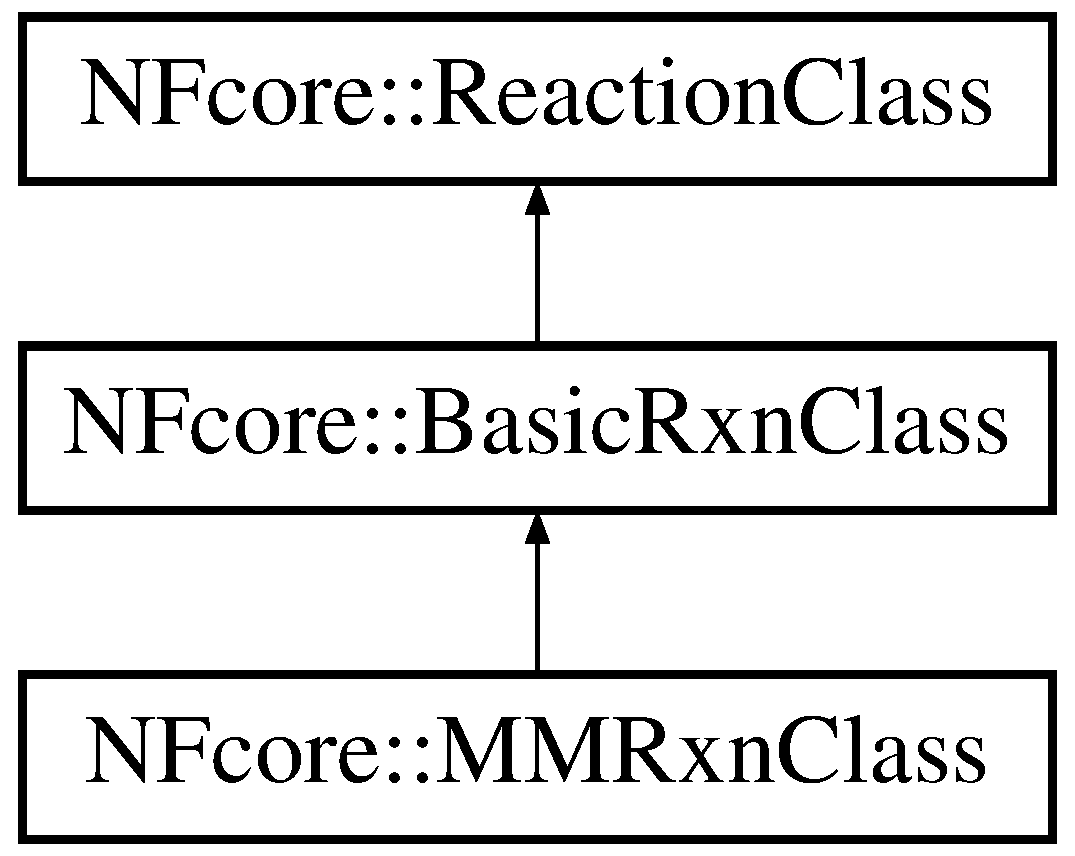
\includegraphics[height=3cm]{classNFcore_1_1MMRxnClass}
\end{center}
\end{figure}
\subsection*{Public Member Functions}
\begin{CompactItemize}
\item 
{\bf MMRxnClass} (string {\bf name}, double {\bf kcat}, double {\bf Km}, {\bf TransformationSet} $\ast${\bf transformationSet})
\item 
virtual {\bf $\sim$MMRxnClass} ()
\item 
virtual double {\bf update\_\-a} ()
\item 
virtual void {\bf printDetails} () const 
\end{CompactItemize}
\subsection*{Protected Attributes}
\begin{CompactItemize}
\item 
double {\bf Km}
\item 
double {\bf kcat}
\item 
double {\bf sFree}
\end{CompactItemize}


\subsection{Constructor \& Destructor Documentation}
\index{NFcore::MMRxnClass@{NFcore::MMRxnClass}!MMRxnClass@{MMRxnClass}}
\index{MMRxnClass@{MMRxnClass}!NFcore::MMRxnClass@{NFcore::MMRxnClass}}
\subsubsection{\setlength{\rightskip}{0pt plus 5cm}MMRxnClass::MMRxnClass (string {\em name}, double {\em kcat}, double {\em Km}, {\bf TransformationSet} $\ast$ {\em transformationSet})}\label{classNFcore_1_1MMRxnClass_8abc5db1c07724df1b7a088c9ea095c5}


\index{NFcore::MMRxnClass@{NFcore::MMRxnClass}!$\sim$MMRxnClass@{$\sim$MMRxnClass}}
\index{$\sim$MMRxnClass@{$\sim$MMRxnClass}!NFcore::MMRxnClass@{NFcore::MMRxnClass}}
\subsubsection{\setlength{\rightskip}{0pt plus 5cm}MMRxnClass::$\sim$MMRxnClass ()\hspace{0.3cm}{\tt  [virtual]}}\label{classNFcore_1_1MMRxnClass_38c689611b5b9503b4b0aebcf9f4fac9}




\subsection{Member Function Documentation}
\index{NFcore::MMRxnClass@{NFcore::MMRxnClass}!update\_\-a@{update\_\-a}}
\index{update\_\-a@{update\_\-a}!NFcore::MMRxnClass@{NFcore::MMRxnClass}}
\subsubsection{\setlength{\rightskip}{0pt plus 5cm}double MMRxnClass::update\_\-a ()\hspace{0.3cm}{\tt  [virtual]}}\label{classNFcore_1_1MMRxnClass_63709cdada0fc7c63125bd2e562f4b42}




Reimplemented from {\bf NFcore::BasicRxnClass} \doxyref{}{p.}{classNFcore_1_1BasicRxnClass_9a679d57f4cfdd184f3bf312ecd20cc6}.\index{NFcore::MMRxnClass@{NFcore::MMRxnClass}!printDetails@{printDetails}}
\index{printDetails@{printDetails}!NFcore::MMRxnClass@{NFcore::MMRxnClass}}
\subsubsection{\setlength{\rightskip}{0pt plus 5cm}void MMRxnClass::printDetails () const\hspace{0.3cm}{\tt  [virtual]}}\label{classNFcore_1_1MMRxnClass_2dc1bbf290be2f3d535954d006efc385}




Reimplemented from {\bf NFcore::ReactionClass} \doxyref{}{p.}{classNFcore_1_1ReactionClass_7944db14780627ea05cf290688a8bfd3}.

\subsection{Member Data Documentation}
\index{NFcore::MMRxnClass@{NFcore::MMRxnClass}!Km@{Km}}
\index{Km@{Km}!NFcore::MMRxnClass@{NFcore::MMRxnClass}}
\subsubsection{\setlength{\rightskip}{0pt plus 5cm}double {\bf NFcore::MMRxnClass::Km}\hspace{0.3cm}{\tt  [protected]}}\label{classNFcore_1_1MMRxnClass_7e4efd8d3df44e2b45085882162e0f72}


\index{NFcore::MMRxnClass@{NFcore::MMRxnClass}!kcat@{kcat}}
\index{kcat@{kcat}!NFcore::MMRxnClass@{NFcore::MMRxnClass}}
\subsubsection{\setlength{\rightskip}{0pt plus 5cm}double {\bf NFcore::MMRxnClass::kcat}\hspace{0.3cm}{\tt  [protected]}}\label{classNFcore_1_1MMRxnClass_9d72aae7237900463c277ee31dd41edd}


\index{NFcore::MMRxnClass@{NFcore::MMRxnClass}!sFree@{sFree}}
\index{sFree@{sFree}!NFcore::MMRxnClass@{NFcore::MMRxnClass}}
\subsubsection{\setlength{\rightskip}{0pt plus 5cm}double {\bf NFcore::MMRxnClass::sFree}\hspace{0.3cm}{\tt  [protected]}}\label{classNFcore_1_1MMRxnClass_31c98a563a88bc8880e7ced28608930c}




The documentation for this class was generated from the following files:\begin{CompactItemize}
\item 
/home/msneddon/eclipse/ganymede\_\-cpp/workspace/NFsim\_\-svn/src/NFreactions/reactions/{\bf reaction.hh}\item 
/home/msneddon/eclipse/ganymede\_\-cpp/workspace/NFsim\_\-svn/src/NFreactions/reactions/{\bf reaction.cpp}\end{CompactItemize}

\section{NFcore::Molecule Class Reference}
\label{classNFcore_1_1Molecule}\index{NFcore::Molecule@{NFcore::Molecule}}
{\tt \#include $<$NFcore.hh$>$}



\subsection{Detailed Description}
Each molecule in the system is represented by an instance of this. 

The base unit of the NFsim program, this class maintains instances of individual objects that exist in the simulation. Molecules are able to interact with their \doxyref{MoleculeType}{p.}{classNFcore_1_1MoleculeType} so that they also 'know' about the reactions and observables they need to keep updated as they react and change states. There are also two static functions which are used to create and delete bonds (bind and unbind). \begin{Desc}
\item[Author:]Michael Sneddon \end{Desc}
\subsection*{Public Member Functions}
\begin{CompactItemize}
\item 
{\bf Molecule} ({\bf MoleculeType} $\ast${\bf parentMoleculeType}, int {\bf listId})
\item 
{\bf $\sim$Molecule} ()
\item 
int {\bf getMolListId} () const 
\item 
string {\bf getMoleculeTypeName} () const 
\item 
{\bf MoleculeType} $\ast$ {\bf getMoleculeType} () const 
\item 
int {\bf getUniqueID} () const 
\item 
bool {\bf isAlive} () const 
\item 
void {\bf setAlive} (bool isAlive)
\item 
void {\bf setComplexID} (int currentComplex)
\item 
int {\bf getComplexID} () const 
\item 
{\bf Complex} $\ast$ {\bf getComplex} () const 
\item 
int {\bf getDegree} ()
\item 
bool {\bf isPopulationType} () const 
\item 
bool {\bf setPopulation} (int count)
\item 
int {\bf getPopulation} () const 
\item 
bool {\bf incrementPopulation} ()
\item 
bool {\bf decrementPopulation} ()
\item 
int {\bf getComponentState} (int cIndex) const 
\item 
int {\bf getComponentIndexOfBond} (int cIndex) const 
\item 
void {\bf setComponentState} (int cIndex, int newValue)
\item 
void {\bf setComponentState} (string cName, int newValue)
\item 
void {\bf setLocalFunctionValue} (double newValue, int localFunctionIndex)
\item 
double {\bf getLocalFunctionValue} (int localFunctionIndex)
\item 
{\bf LocalFunction} $\ast$ {\bf getLocalFunction} (int localFunctionIndex)
\item 
void {\bf setUpLocalFunctionList} ()
\item 
bool {\bf isBindingSiteOpen} (int bIndex) const 
\item 
bool {\bf isBindingSiteBonded} (int bIndex) const 
\item 
{\bf Molecule} $\ast$ {\bf getBondedMolecule} (int bSiteIndex) const 
\item 
int {\bf getBondedMoleculeBindingSiteIndex} (int cIndex) const 
\item 
int {\bf getRxnListMappingId} (int rxnIndex) const 
\item 
void {\bf setRxnListMappingId} (int rxnIndex, int {\bf rxnListMappingId})
\item 
void {\bf setBondTo} ({\bf Molecule} $\ast$m2, int bindingSiteIndex)
\item 
void {\bf moveToNewComplex} (int newComplexID)
\item 
void {\bf traverseBondedNeighborhood} (list$<$ {\bf Molecule} $\ast$ $>$ \&members, int traversalLimit)
\item 
void {\bf depthFirstSearch} (list$<$ {\bf Molecule} $\ast$ $>$ \&members)
\item 
void {\bf prepareForSimulation} ()
\item 
void {\bf updateRxnMembership} ()
\item 
void {\bf removeFromObservables} ()
\item 
void {\bf addToObservables} ()
\item 
void {\bf updateTypeIIFunctions} ()
\item 
void {\bf updateDORRxnValues} ()
\item 
void {\bf printDetails} ()
\item 
void {\bf printDetails} (ostream \&o)
\item 
int {\bf isObs} (int oIndex) const 
\item 
void {\bf setIsObs} (int oIndex, int isObs)
\end{CompactItemize}
\subsection*{Static Public Member Functions}
\begin{CompactItemize}
\item 
static void {\bf bind} ({\bf Molecule} $\ast$m1, int cIndex1, {\bf Molecule} $\ast$m2, int cIndex2)
\item 
static void {\bf bind} ({\bf Molecule} $\ast$m1, string compName1, {\bf Molecule} $\ast$m2, string compName2)
\item 
static void {\bf unbind} ({\bf Molecule} $\ast$m1, int bSiteIndex)
\item 
static void {\bf unbind} ({\bf Molecule} $\ast$m1, char $\ast$bSiteName)
\item 
static void {\bf breadthFirstSearch} (list$<$ {\bf Molecule} $\ast$ $>$ \&members, {\bf Molecule} $\ast$m, int depth)
\item 
static void {\bf printMoleculeList} (list$<$ {\bf Molecule} $\ast$ $>$ \&members)
\item 
static int {\bf getUniqueIdCount} ()
\end{CompactItemize}
\subsection*{Public Attributes}
\begin{CompactItemize}
\item 
bool {\bf hasVisitedMolecule}
\item 
bool $\ast$ {\bf hasVisitedBond}
\item 
{\bf TemplateMolecule} $\ast$ {\bf isMatchedTo}
\item 
bool {\bf hasEvaluatedMolecule}
\end{CompactItemize}
\subsection*{Static Public Attributes}
\begin{CompactItemize}
\item 
static const int {\bf NOT\_\-IN\_\-RXN} = -1
\item 
static const int {\bf NOSTATE} = -1
\item 
static const int {\bf NOBOND} = 0
\item 
static const int {\bf NOINDEX} = -1
\end{CompactItemize}
\subsection*{Protected Attributes}
\begin{CompactItemize}
\item 
bool {\bf isPrepared}
\item 
bool {\bf isAliveInSim}
\item 
int {\bf ID\_\-complex}
\item 
int {\bf ID\_\-type}
\item 
int {\bf ID\_\-unique}
\item 
int {\bf listId}
\item 
{\bf MoleculeType} $\ast$ {\bf parentMoleculeType}
\item 
bool {\bf useComplex}
\item 
int {\bf population\_\-count}
\item 
int $\ast$ {\bf component}
\item 
int {\bf numOfComponents}
\item 
{\bf Molecule} $\ast$$\ast$ {\bf bond}
\item 
int $\ast$ {\bf indexOfBond}
\item 
double $\ast$ {\bf localFunctionValues}
\item 
int $\ast$ {\bf isObservable}
\item 
int $\ast$ {\bf rxnListMappingId}
\item 
int {\bf nReactions}
\end{CompactItemize}
\subsection*{Static Protected Attributes}
\begin{CompactItemize}
\item 
static int {\bf uniqueIdCount} = 0
\end{CompactItemize}


\subsection{Constructor \& Destructor Documentation}
\index{NFcore::Molecule@{NFcore::Molecule}!Molecule@{Molecule}}
\index{Molecule@{Molecule}!NFcore::Molecule@{NFcore::Molecule}}
\subsubsection{\setlength{\rightskip}{0pt plus 5cm}Molecule::Molecule ({\bf MoleculeType} $\ast$ {\em parentMoleculeType}, int {\em listId})}\label{classNFcore_1_1Molecule_09f19b608d8bcc051b61e2ab1fffa207}


\index{NFcore::Molecule@{NFcore::Molecule}!$\sim$Molecule@{$\sim$Molecule}}
\index{$\sim$Molecule@{$\sim$Molecule}!NFcore::Molecule@{NFcore::Molecule}}
\subsubsection{\setlength{\rightskip}{0pt plus 5cm}Molecule::$\sim$Molecule ()}\label{classNFcore_1_1Molecule_1ff980b574a62526abff3d631c83bf94}




\subsection{Member Function Documentation}
\index{NFcore::Molecule@{NFcore::Molecule}!getMolListId@{getMolListId}}
\index{getMolListId@{getMolListId}!NFcore::Molecule@{NFcore::Molecule}}
\subsubsection{\setlength{\rightskip}{0pt plus 5cm}int NFcore::Molecule::getMolListId () const\hspace{0.3cm}{\tt  [inline]}}\label{classNFcore_1_1Molecule_5b8fa63376968f8905e7979e8648647b}


\index{NFcore::Molecule@{NFcore::Molecule}!getMoleculeTypeName@{getMoleculeTypeName}}
\index{getMoleculeTypeName@{getMoleculeTypeName}!NFcore::Molecule@{NFcore::Molecule}}
\subsubsection{\setlength{\rightskip}{0pt plus 5cm}string NFcore::Molecule::getMoleculeTypeName () const\hspace{0.3cm}{\tt  [inline]}}\label{classNFcore_1_1Molecule_54b335a50f427d3af013b3f833552c78}


\index{NFcore::Molecule@{NFcore::Molecule}!getMoleculeType@{getMoleculeType}}
\index{getMoleculeType@{getMoleculeType}!NFcore::Molecule@{NFcore::Molecule}}
\subsubsection{\setlength{\rightskip}{0pt plus 5cm}{\bf MoleculeType}$\ast$ NFcore::Molecule::getMoleculeType () const\hspace{0.3cm}{\tt  [inline]}}\label{classNFcore_1_1Molecule_7b3552809de0a478b64c4eb4ca4096d5}


\index{NFcore::Molecule@{NFcore::Molecule}!getUniqueID@{getUniqueID}}
\index{getUniqueID@{getUniqueID}!NFcore::Molecule@{NFcore::Molecule}}
\subsubsection{\setlength{\rightskip}{0pt plus 5cm}int NFcore::Molecule::getUniqueID () const\hspace{0.3cm}{\tt  [inline]}}\label{classNFcore_1_1Molecule_bdc033d5a74f5453712ac9ec36b0564f}


\index{NFcore::Molecule@{NFcore::Molecule}!isAlive@{isAlive}}
\index{isAlive@{isAlive}!NFcore::Molecule@{NFcore::Molecule}}
\subsubsection{\setlength{\rightskip}{0pt plus 5cm}bool NFcore::Molecule::isAlive () const\hspace{0.3cm}{\tt  [inline]}}\label{classNFcore_1_1Molecule_026c2150941021241376f31ab5cdfa8b}


\index{NFcore::Molecule@{NFcore::Molecule}!setAlive@{setAlive}}
\index{setAlive@{setAlive}!NFcore::Molecule@{NFcore::Molecule}}
\subsubsection{\setlength{\rightskip}{0pt plus 5cm}void NFcore::Molecule::setAlive (bool {\em isAlive})\hspace{0.3cm}{\tt  [inline]}}\label{classNFcore_1_1Molecule_70a78e2f3cc4020ab0224e03f722f568}


\index{NFcore::Molecule@{NFcore::Molecule}!setComplexID@{setComplexID}}
\index{setComplexID@{setComplexID}!NFcore::Molecule@{NFcore::Molecule}}
\subsubsection{\setlength{\rightskip}{0pt plus 5cm}void NFcore::Molecule::setComplexID (int {\em currentComplex})\hspace{0.3cm}{\tt  [inline]}}\label{classNFcore_1_1Molecule_69465045c57bb005157fc2aea3efb39d}


\index{NFcore::Molecule@{NFcore::Molecule}!getComplexID@{getComplexID}}
\index{getComplexID@{getComplexID}!NFcore::Molecule@{NFcore::Molecule}}
\subsubsection{\setlength{\rightskip}{0pt plus 5cm}int NFcore::Molecule::getComplexID () const\hspace{0.3cm}{\tt  [inline]}}\label{classNFcore_1_1Molecule_16f3f77ac1f62468a6f77be13f224b2b}


\index{NFcore::Molecule@{NFcore::Molecule}!getComplex@{getComplex}}
\index{getComplex@{getComplex}!NFcore::Molecule@{NFcore::Molecule}}
\subsubsection{\setlength{\rightskip}{0pt plus 5cm}{\bf Complex}$\ast$ NFcore::Molecule::getComplex () const\hspace{0.3cm}{\tt  [inline]}}\label{classNFcore_1_1Molecule_42b4fdfe04c8da86bfd2ac5f4a93492d}


\index{NFcore::Molecule@{NFcore::Molecule}!getDegree@{getDegree}}
\index{getDegree@{getDegree}!NFcore::Molecule@{NFcore::Molecule}}
\subsubsection{\setlength{\rightskip}{0pt plus 5cm}int Molecule::getDegree ()}\label{classNFcore_1_1Molecule_390f0d1223bdd2ab075b25993902a520}


\index{NFcore::Molecule@{NFcore::Molecule}!isPopulationType@{isPopulationType}}
\index{isPopulationType@{isPopulationType}!NFcore::Molecule@{NFcore::Molecule}}
\subsubsection{\setlength{\rightskip}{0pt plus 5cm}bool NFcore::Molecule::isPopulationType () const\hspace{0.3cm}{\tt  [inline]}}\label{classNFcore_1_1Molecule_16b6745c6533c31333334dc3d39417e4}


\index{NFcore::Molecule@{NFcore::Molecule}!setPopulation@{setPopulation}}
\index{setPopulation@{setPopulation}!NFcore::Molecule@{NFcore::Molecule}}
\subsubsection{\setlength{\rightskip}{0pt plus 5cm}bool Molecule::setPopulation (int {\em count})}\label{classNFcore_1_1Molecule_efdeb81a3b9d98a8644db2e1acd59404}


\index{NFcore::Molecule@{NFcore::Molecule}!getPopulation@{getPopulation}}
\index{getPopulation@{getPopulation}!NFcore::Molecule@{NFcore::Molecule}}
\subsubsection{\setlength{\rightskip}{0pt plus 5cm}int Molecule::getPopulation () const}\label{classNFcore_1_1Molecule_912defe8c71ea04e15b94d161a50a61c}


\index{NFcore::Molecule@{NFcore::Molecule}!incrementPopulation@{incrementPopulation}}
\index{incrementPopulation@{incrementPopulation}!NFcore::Molecule@{NFcore::Molecule}}
\subsubsection{\setlength{\rightskip}{0pt plus 5cm}bool Molecule::incrementPopulation ()}\label{classNFcore_1_1Molecule_854b5ead187df0c2aeb04b208ad4c0b0}


\index{NFcore::Molecule@{NFcore::Molecule}!decrementPopulation@{decrementPopulation}}
\index{decrementPopulation@{decrementPopulation}!NFcore::Molecule@{NFcore::Molecule}}
\subsubsection{\setlength{\rightskip}{0pt plus 5cm}bool Molecule::decrementPopulation ()}\label{classNFcore_1_1Molecule_eda502a7eb99b0b319491ed416000b92}


\index{NFcore::Molecule@{NFcore::Molecule}!getComponentState@{getComponentState}}
\index{getComponentState@{getComponentState}!NFcore::Molecule@{NFcore::Molecule}}
\subsubsection{\setlength{\rightskip}{0pt plus 5cm}int NFcore::Molecule::getComponentState (int {\em cIndex}) const\hspace{0.3cm}{\tt  [inline]}}\label{classNFcore_1_1Molecule_7b79c8463c9c4dc88549aa74ba7179cc}


\index{NFcore::Molecule@{NFcore::Molecule}!getComponentIndexOfBond@{getComponentIndexOfBond}}
\index{getComponentIndexOfBond@{getComponentIndexOfBond}!NFcore::Molecule@{NFcore::Molecule}}
\subsubsection{\setlength{\rightskip}{0pt plus 5cm}int NFcore::Molecule::getComponentIndexOfBond (int {\em cIndex}) const\hspace{0.3cm}{\tt  [inline]}}\label{classNFcore_1_1Molecule_644b32b9f8609ee675f2ecc4f458d678}


\index{NFcore::Molecule@{NFcore::Molecule}!setComponentState@{setComponentState}}
\index{setComponentState@{setComponentState}!NFcore::Molecule@{NFcore::Molecule}}
\subsubsection{\setlength{\rightskip}{0pt plus 5cm}void Molecule::setComponentState (int {\em cIndex}, int {\em newValue})}\label{classNFcore_1_1Molecule_0eb79f69d465c6407b078f59465d1413}


\index{NFcore::Molecule@{NFcore::Molecule}!setComponentState@{setComponentState}}
\index{setComponentState@{setComponentState}!NFcore::Molecule@{NFcore::Molecule}}
\subsubsection{\setlength{\rightskip}{0pt plus 5cm}void Molecule::setComponentState (string {\em cName}, int {\em newValue})}\label{classNFcore_1_1Molecule_7e96ad7ebb9ebde9324b1f069f8078d4}


\index{NFcore::Molecule@{NFcore::Molecule}!setLocalFunctionValue@{setLocalFunctionValue}}
\index{setLocalFunctionValue@{setLocalFunctionValue}!NFcore::Molecule@{NFcore::Molecule}}
\subsubsection{\setlength{\rightskip}{0pt plus 5cm}void Molecule::setLocalFunctionValue (double {\em newValue}, int {\em localFunctionIndex})}\label{classNFcore_1_1Molecule_d5f5d4f6094fc06d21ee7834dd1d6ca5}


\index{NFcore::Molecule@{NFcore::Molecule}!getLocalFunctionValue@{getLocalFunctionValue}}
\index{getLocalFunctionValue@{getLocalFunctionValue}!NFcore::Molecule@{NFcore::Molecule}}
\subsubsection{\setlength{\rightskip}{0pt plus 5cm}double Molecule::getLocalFunctionValue (int {\em localFunctionIndex})}\label{classNFcore_1_1Molecule_10dc17ce9638bbfe58693a428c95e3a8}


\index{NFcore::Molecule@{NFcore::Molecule}!getLocalFunction@{getLocalFunction}}
\index{getLocalFunction@{getLocalFunction}!NFcore::Molecule@{NFcore::Molecule}}
\subsubsection{\setlength{\rightskip}{0pt plus 5cm}{\bf LocalFunction} $\ast$ Molecule::getLocalFunction (int {\em localFunctionIndex})}\label{classNFcore_1_1Molecule_b85c118563895e50c619fb584c2ace5b}


\index{NFcore::Molecule@{NFcore::Molecule}!setUpLocalFunctionList@{setUpLocalFunctionList}}
\index{setUpLocalFunctionList@{setUpLocalFunctionList}!NFcore::Molecule@{NFcore::Molecule}}
\subsubsection{\setlength{\rightskip}{0pt plus 5cm}void Molecule::setUpLocalFunctionList ()}\label{classNFcore_1_1Molecule_74b2a51b8799923556e413a4955a3926}


\index{NFcore::Molecule@{NFcore::Molecule}!isBindingSiteOpen@{isBindingSiteOpen}}
\index{isBindingSiteOpen@{isBindingSiteOpen}!NFcore::Molecule@{NFcore::Molecule}}
\subsubsection{\setlength{\rightskip}{0pt plus 5cm}bool Molecule::isBindingSiteOpen (int {\em bIndex}) const}\label{classNFcore_1_1Molecule_80db66e3d3582f040a363fc625130a88}


\index{NFcore::Molecule@{NFcore::Molecule}!isBindingSiteBonded@{isBindingSiteBonded}}
\index{isBindingSiteBonded@{isBindingSiteBonded}!NFcore::Molecule@{NFcore::Molecule}}
\subsubsection{\setlength{\rightskip}{0pt plus 5cm}bool Molecule::isBindingSiteBonded (int {\em bIndex}) const}\label{classNFcore_1_1Molecule_4e50fb96e3a9cbd47d8ae7156f2a10bc}


\index{NFcore::Molecule@{NFcore::Molecule}!getBondedMolecule@{getBondedMolecule}}
\index{getBondedMolecule@{getBondedMolecule}!NFcore::Molecule@{NFcore::Molecule}}
\subsubsection{\setlength{\rightskip}{0pt plus 5cm}{\bf Molecule} $\ast$ Molecule::getBondedMolecule (int {\em bSiteIndex}) const}\label{classNFcore_1_1Molecule_7833785f509d95b6a97b299526d1d6e4}


\index{NFcore::Molecule@{NFcore::Molecule}!getBondedMoleculeBindingSiteIndex@{getBondedMoleculeBindingSiteIndex}}
\index{getBondedMoleculeBindingSiteIndex@{getBondedMoleculeBindingSiteIndex}!NFcore::Molecule@{NFcore::Molecule}}
\subsubsection{\setlength{\rightskip}{0pt plus 5cm}int Molecule::getBondedMoleculeBindingSiteIndex (int {\em cIndex}) const}\label{classNFcore_1_1Molecule_bcc94973b4d615d2d8ade51b782b0e35}


\index{NFcore::Molecule@{NFcore::Molecule}!getRxnListMappingId@{getRxnListMappingId}}
\index{getRxnListMappingId@{getRxnListMappingId}!NFcore::Molecule@{NFcore::Molecule}}
\subsubsection{\setlength{\rightskip}{0pt plus 5cm}int NFcore::Molecule::getRxnListMappingId (int {\em rxnIndex}) const\hspace{0.3cm}{\tt  [inline]}}\label{classNFcore_1_1Molecule_a352c3ff40bb38555c772124de0f0ac8}


\index{NFcore::Molecule@{NFcore::Molecule}!setRxnListMappingId@{setRxnListMappingId}}
\index{setRxnListMappingId@{setRxnListMappingId}!NFcore::Molecule@{NFcore::Molecule}}
\subsubsection{\setlength{\rightskip}{0pt plus 5cm}void NFcore::Molecule::setRxnListMappingId (int {\em rxnIndex}, int {\em rxnListMappingId})\hspace{0.3cm}{\tt  [inline]}}\label{classNFcore_1_1Molecule_9cf1eae438fc06f9e70d541e4a0b32d5}


\index{NFcore::Molecule@{NFcore::Molecule}!setBondTo@{setBondTo}}
\index{setBondTo@{setBondTo}!NFcore::Molecule@{NFcore::Molecule}}
\subsubsection{\setlength{\rightskip}{0pt plus 5cm}void NFcore::Molecule::setBondTo ({\bf Molecule} $\ast$ {\em m2}, int {\em bindingSiteIndex})}\label{classNFcore_1_1Molecule_83f24f5163f0521e1ce77bb8aef2ac97}


\index{NFcore::Molecule@{NFcore::Molecule}!moveToNewComplex@{moveToNewComplex}}
\index{moveToNewComplex@{moveToNewComplex}!NFcore::Molecule@{NFcore::Molecule}}
\subsubsection{\setlength{\rightskip}{0pt plus 5cm}void NFcore::Molecule::moveToNewComplex (int {\em newComplexID})\hspace{0.3cm}{\tt  [inline]}}\label{classNFcore_1_1Molecule_691daed6bab7b13dd5bfe6da41a8ab48}


\index{NFcore::Molecule@{NFcore::Molecule}!bind@{bind}}
\index{bind@{bind}!NFcore::Molecule@{NFcore::Molecule}}
\subsubsection{\setlength{\rightskip}{0pt plus 5cm}void Molecule::bind ({\bf Molecule} $\ast$ {\em m1}, int {\em cIndex1}, {\bf Molecule} $\ast$ {\em m2}, int {\em cIndex2})\hspace{0.3cm}{\tt  [static]}}\label{classNFcore_1_1Molecule_776a89ff6affb64d02f180403207d0ac}


\index{NFcore::Molecule@{NFcore::Molecule}!bind@{bind}}
\index{bind@{bind}!NFcore::Molecule@{NFcore::Molecule}}
\subsubsection{\setlength{\rightskip}{0pt plus 5cm}void Molecule::bind ({\bf Molecule} $\ast$ {\em m1}, string {\em compName1}, {\bf Molecule} $\ast$ {\em m2}, string {\em compName2})\hspace{0.3cm}{\tt  [static]}}\label{classNFcore_1_1Molecule_7a43a97c3f1baad5eb5e11b91683d782}


\index{NFcore::Molecule@{NFcore::Molecule}!unbind@{unbind}}
\index{unbind@{unbind}!NFcore::Molecule@{NFcore::Molecule}}
\subsubsection{\setlength{\rightskip}{0pt plus 5cm}void Molecule::unbind ({\bf Molecule} $\ast$ {\em m1}, int {\em bSiteIndex})\hspace{0.3cm}{\tt  [static]}}\label{classNFcore_1_1Molecule_e37cae25c4e0e544ae0b9b9930ae309b}


\index{NFcore::Molecule@{NFcore::Molecule}!unbind@{unbind}}
\index{unbind@{unbind}!NFcore::Molecule@{NFcore::Molecule}}
\subsubsection{\setlength{\rightskip}{0pt plus 5cm}void Molecule::unbind ({\bf Molecule} $\ast$ {\em m1}, char $\ast$ {\em bSiteName})\hspace{0.3cm}{\tt  [static]}}\label{classNFcore_1_1Molecule_b29bc47ee1304d31173dc00af20bbafd}


\index{NFcore::Molecule@{NFcore::Molecule}!traverseBondedNeighborhood@{traverseBondedNeighborhood}}
\index{traverseBondedNeighborhood@{traverseBondedNeighborhood}!NFcore::Molecule@{NFcore::Molecule}}
\subsubsection{\setlength{\rightskip}{0pt plus 5cm}void Molecule::traverseBondedNeighborhood (list$<$ {\bf Molecule} $\ast$ $>$ \& {\em members}, int {\em traversalLimit})}\label{classNFcore_1_1Molecule_410a708dc5a802794c49a1b547e220cb}


\index{NFcore::Molecule@{NFcore::Molecule}!breadthFirstSearch@{breadthFirstSearch}}
\index{breadthFirstSearch@{breadthFirstSearch}!NFcore::Molecule@{NFcore::Molecule}}
\subsubsection{\setlength{\rightskip}{0pt plus 5cm}void Molecule::breadthFirstSearch (list$<$ {\bf Molecule} $\ast$ $>$ \& {\em members}, {\bf Molecule} $\ast$ {\em m}, int {\em depth})\hspace{0.3cm}{\tt  [static]}}\label{classNFcore_1_1Molecule_6242f0f2226f92690f67d2d60e39209e}


\index{NFcore::Molecule@{NFcore::Molecule}!depthFirstSearch@{depthFirstSearch}}
\index{depthFirstSearch@{depthFirstSearch}!NFcore::Molecule@{NFcore::Molecule}}
\subsubsection{\setlength{\rightskip}{0pt plus 5cm}void Molecule::depthFirstSearch (list$<$ {\bf Molecule} $\ast$ $>$ \& {\em members})}\label{classNFcore_1_1Molecule_20fc55c24b214a07d4dd10b966c1dcb7}


\index{NFcore::Molecule@{NFcore::Molecule}!prepareForSimulation@{prepareForSimulation}}
\index{prepareForSimulation@{prepareForSimulation}!NFcore::Molecule@{NFcore::Molecule}}
\subsubsection{\setlength{\rightskip}{0pt plus 5cm}void Molecule::prepareForSimulation ()}\label{classNFcore_1_1Molecule_e7791ea7d5c718e769355885264ed27c}


\index{NFcore::Molecule@{NFcore::Molecule}!updateRxnMembership@{updateRxnMembership}}
\index{updateRxnMembership@{updateRxnMembership}!NFcore::Molecule@{NFcore::Molecule}}
\subsubsection{\setlength{\rightskip}{0pt plus 5cm}void Molecule::updateRxnMembership ()}\label{classNFcore_1_1Molecule_418a61a3ccd7c37c53e30cbe90d35a94}


\index{NFcore::Molecule@{NFcore::Molecule}!removeFromObservables@{removeFromObservables}}
\index{removeFromObservables@{removeFromObservables}!NFcore::Molecule@{NFcore::Molecule}}
\subsubsection{\setlength{\rightskip}{0pt plus 5cm}void Molecule::removeFromObservables ()}\label{classNFcore_1_1Molecule_b996dfd73160b4e2e0f060db729663c8}


\index{NFcore::Molecule@{NFcore::Molecule}!addToObservables@{addToObservables}}
\index{addToObservables@{addToObservables}!NFcore::Molecule@{NFcore::Molecule}}
\subsubsection{\setlength{\rightskip}{0pt plus 5cm}void Molecule::addToObservables ()}\label{classNFcore_1_1Molecule_e971b5fde9399fab335e572c02ba253b}


\index{NFcore::Molecule@{NFcore::Molecule}!updateTypeIIFunctions@{updateTypeIIFunctions}}
\index{updateTypeIIFunctions@{updateTypeIIFunctions}!NFcore::Molecule@{NFcore::Molecule}}
\subsubsection{\setlength{\rightskip}{0pt plus 5cm}void Molecule::updateTypeIIFunctions ()}\label{classNFcore_1_1Molecule_6339cd45a1ebb484a93bec719a2d0c76}


\index{NFcore::Molecule@{NFcore::Molecule}!updateDORRxnValues@{updateDORRxnValues}}
\index{updateDORRxnValues@{updateDORRxnValues}!NFcore::Molecule@{NFcore::Molecule}}
\subsubsection{\setlength{\rightskip}{0pt plus 5cm}void Molecule::updateDORRxnValues ()}\label{classNFcore_1_1Molecule_2ed78fda19237bbfdc179530cce22e27}


\index{NFcore::Molecule@{NFcore::Molecule}!printDetails@{printDetails}}
\index{printDetails@{printDetails}!NFcore::Molecule@{NFcore::Molecule}}
\subsubsection{\setlength{\rightskip}{0pt plus 5cm}void Molecule::printDetails ()}\label{classNFcore_1_1Molecule_5abd4eb1ec78c0877a0e1ae4b085866e}


\index{NFcore::Molecule@{NFcore::Molecule}!printDetails@{printDetails}}
\index{printDetails@{printDetails}!NFcore::Molecule@{NFcore::Molecule}}
\subsubsection{\setlength{\rightskip}{0pt plus 5cm}void Molecule::printDetails (ostream \& {\em o})}\label{classNFcore_1_1Molecule_492aea103ce2471d82cf2571a1263f04}


\index{NFcore::Molecule@{NFcore::Molecule}!printMoleculeList@{printMoleculeList}}
\index{printMoleculeList@{printMoleculeList}!NFcore::Molecule@{NFcore::Molecule}}
\subsubsection{\setlength{\rightskip}{0pt plus 5cm}void Molecule::printMoleculeList (list$<$ {\bf Molecule} $\ast$ $>$ \& {\em members})\hspace{0.3cm}{\tt  [static]}}\label{classNFcore_1_1Molecule_6773f433bfb5546ddc0e8546aaec9817}


\index{NFcore::Molecule@{NFcore::Molecule}!getUniqueIdCount@{getUniqueIdCount}}
\index{getUniqueIdCount@{getUniqueIdCount}!NFcore::Molecule@{NFcore::Molecule}}
\subsubsection{\setlength{\rightskip}{0pt plus 5cm}static int NFcore::Molecule::getUniqueIdCount ()\hspace{0.3cm}{\tt  [inline, static]}}\label{classNFcore_1_1Molecule_e11f21aabfaa393b34f680bbbee6b20d}


\index{NFcore::Molecule@{NFcore::Molecule}!isObs@{isObs}}
\index{isObs@{isObs}!NFcore::Molecule@{NFcore::Molecule}}
\subsubsection{\setlength{\rightskip}{0pt plus 5cm}int NFcore::Molecule::isObs (int {\em oIndex}) const\hspace{0.3cm}{\tt  [inline]}}\label{classNFcore_1_1Molecule_7f72bdf2e57d118402cf66037ecdd7a7}


\index{NFcore::Molecule@{NFcore::Molecule}!setIsObs@{setIsObs}}
\index{setIsObs@{setIsObs}!NFcore::Molecule@{NFcore::Molecule}}
\subsubsection{\setlength{\rightskip}{0pt plus 5cm}void NFcore::Molecule::setIsObs (int {\em oIndex}, int {\em isObs})\hspace{0.3cm}{\tt  [inline]}}\label{classNFcore_1_1Molecule_07ebe50f8f57c9d2ee2c313b1c21d25e}




\subsection{Member Data Documentation}
\index{NFcore::Molecule@{NFcore::Molecule}!NOT\_\-IN\_\-RXN@{NOT\_\-IN\_\-RXN}}
\index{NOT\_\-IN\_\-RXN@{NOT\_\-IN\_\-RXN}!NFcore::Molecule@{NFcore::Molecule}}
\subsubsection{\setlength{\rightskip}{0pt plus 5cm}const int {\bf NFcore::Molecule::NOT\_\-IN\_\-RXN} = -1\hspace{0.3cm}{\tt  [static]}}\label{classNFcore_1_1Molecule_b17b0ab2e0bd3746c065351e346f4ffe}


\index{NFcore::Molecule@{NFcore::Molecule}!hasVisitedMolecule@{hasVisitedMolecule}}
\index{hasVisitedMolecule@{hasVisitedMolecule}!NFcore::Molecule@{NFcore::Molecule}}
\subsubsection{\setlength{\rightskip}{0pt plus 5cm}bool {\bf NFcore::Molecule::hasVisitedMolecule}}\label{classNFcore_1_1Molecule_e828ebe80d90495cb772bde29177166e}


\index{NFcore::Molecule@{NFcore::Molecule}!hasVisitedBond@{hasVisitedBond}}
\index{hasVisitedBond@{hasVisitedBond}!NFcore::Molecule@{NFcore::Molecule}}
\subsubsection{\setlength{\rightskip}{0pt plus 5cm}bool$\ast$ {\bf NFcore::Molecule::hasVisitedBond}}\label{classNFcore_1_1Molecule_f06428c674091090c7cc647e72bbe031}


\index{NFcore::Molecule@{NFcore::Molecule}!isMatchedTo@{isMatchedTo}}
\index{isMatchedTo@{isMatchedTo}!NFcore::Molecule@{NFcore::Molecule}}
\subsubsection{\setlength{\rightskip}{0pt plus 5cm}{\bf TemplateMolecule}$\ast$ {\bf NFcore::Molecule::isMatchedTo}}\label{classNFcore_1_1Molecule_080156e6c2368bb8c2ea5c5eac80a7ed}


\index{NFcore::Molecule@{NFcore::Molecule}!hasEvaluatedMolecule@{hasEvaluatedMolecule}}
\index{hasEvaluatedMolecule@{hasEvaluatedMolecule}!NFcore::Molecule@{NFcore::Molecule}}
\subsubsection{\setlength{\rightskip}{0pt plus 5cm}bool {\bf NFcore::Molecule::hasEvaluatedMolecule}}\label{classNFcore_1_1Molecule_ea3516e9686a0b8f2ee867956cc31c3c}


\index{NFcore::Molecule@{NFcore::Molecule}!NOSTATE@{NOSTATE}}
\index{NOSTATE@{NOSTATE}!NFcore::Molecule@{NFcore::Molecule}}
\subsubsection{\setlength{\rightskip}{0pt plus 5cm}const int {\bf NFcore::Molecule::NOSTATE} = -1\hspace{0.3cm}{\tt  [static]}}\label{classNFcore_1_1Molecule_6909d5d11595ba857c28e382a81526b8}


\index{NFcore::Molecule@{NFcore::Molecule}!NOBOND@{NOBOND}}
\index{NOBOND@{NOBOND}!NFcore::Molecule@{NFcore::Molecule}}
\subsubsection{\setlength{\rightskip}{0pt plus 5cm}const int {\bf NFcore::Molecule::NOBOND} = 0\hspace{0.3cm}{\tt  [static]}}\label{classNFcore_1_1Molecule_2b8a424459016c1e580029e7170ce167}


\index{NFcore::Molecule@{NFcore::Molecule}!NOINDEX@{NOINDEX}}
\index{NOINDEX@{NOINDEX}!NFcore::Molecule@{NFcore::Molecule}}
\subsubsection{\setlength{\rightskip}{0pt plus 5cm}const int {\bf NFcore::Molecule::NOINDEX} = -1\hspace{0.3cm}{\tt  [static]}}\label{classNFcore_1_1Molecule_df16a8aa5b8b53462e2d569eec7f2e87}


\index{NFcore::Molecule@{NFcore::Molecule}!isPrepared@{isPrepared}}
\index{isPrepared@{isPrepared}!NFcore::Molecule@{NFcore::Molecule}}
\subsubsection{\setlength{\rightskip}{0pt plus 5cm}bool {\bf NFcore::Molecule::isPrepared}\hspace{0.3cm}{\tt  [protected]}}\label{classNFcore_1_1Molecule_74d0c636185f07f1d8dc8fe75f67bc5f}


\index{NFcore::Molecule@{NFcore::Molecule}!isAliveInSim@{isAliveInSim}}
\index{isAliveInSim@{isAliveInSim}!NFcore::Molecule@{NFcore::Molecule}}
\subsubsection{\setlength{\rightskip}{0pt plus 5cm}bool {\bf NFcore::Molecule::isAliveInSim}\hspace{0.3cm}{\tt  [protected]}}\label{classNFcore_1_1Molecule_426236fe8eb31ab69e4729e83c360689}


\index{NFcore::Molecule@{NFcore::Molecule}!ID\_\-complex@{ID\_\-complex}}
\index{ID\_\-complex@{ID\_\-complex}!NFcore::Molecule@{NFcore::Molecule}}
\subsubsection{\setlength{\rightskip}{0pt plus 5cm}int {\bf NFcore::Molecule::ID\_\-complex}\hspace{0.3cm}{\tt  [protected]}}\label{classNFcore_1_1Molecule_4f60e43c6a3dd9fe030dbb46e4cecec3}


\index{NFcore::Molecule@{NFcore::Molecule}!ID\_\-type@{ID\_\-type}}
\index{ID\_\-type@{ID\_\-type}!NFcore::Molecule@{NFcore::Molecule}}
\subsubsection{\setlength{\rightskip}{0pt plus 5cm}int {\bf NFcore::Molecule::ID\_\-type}\hspace{0.3cm}{\tt  [protected]}}\label{classNFcore_1_1Molecule_8d3189072332d25bb33310dba5018a6e}


\index{NFcore::Molecule@{NFcore::Molecule}!ID\_\-unique@{ID\_\-unique}}
\index{ID\_\-unique@{ID\_\-unique}!NFcore::Molecule@{NFcore::Molecule}}
\subsubsection{\setlength{\rightskip}{0pt plus 5cm}int {\bf NFcore::Molecule::ID\_\-unique}\hspace{0.3cm}{\tt  [protected]}}\label{classNFcore_1_1Molecule_df1361fab7ec14d70ee6956f0a3aeb1b}


\index{NFcore::Molecule@{NFcore::Molecule}!listId@{listId}}
\index{listId@{listId}!NFcore::Molecule@{NFcore::Molecule}}
\subsubsection{\setlength{\rightskip}{0pt plus 5cm}int {\bf NFcore::Molecule::listId}\hspace{0.3cm}{\tt  [protected]}}\label{classNFcore_1_1Molecule_6910e617031aff17cbe1f33d1bf763b8}


\index{NFcore::Molecule@{NFcore::Molecule}!uniqueIdCount@{uniqueIdCount}}
\index{uniqueIdCount@{uniqueIdCount}!NFcore::Molecule@{NFcore::Molecule}}
\subsubsection{\setlength{\rightskip}{0pt plus 5cm}int {\bf Molecule::uniqueIdCount} = 0\hspace{0.3cm}{\tt  [static, protected]}}\label{classNFcore_1_1Molecule_48087dabb110f4ca4bcb40cae1916f7d}


\index{NFcore::Molecule@{NFcore::Molecule}!parentMoleculeType@{parentMoleculeType}}
\index{parentMoleculeType@{parentMoleculeType}!NFcore::Molecule@{NFcore::Molecule}}
\subsubsection{\setlength{\rightskip}{0pt plus 5cm}{\bf MoleculeType}$\ast$ {\bf NFcore::Molecule::parentMoleculeType}\hspace{0.3cm}{\tt  [protected]}}\label{classNFcore_1_1Molecule_ef848f04c27d380beb9044880f473268}


\index{NFcore::Molecule@{NFcore::Molecule}!useComplex@{useComplex}}
\index{useComplex@{useComplex}!NFcore::Molecule@{NFcore::Molecule}}
\subsubsection{\setlength{\rightskip}{0pt plus 5cm}bool {\bf NFcore::Molecule::useComplex}\hspace{0.3cm}{\tt  [protected]}}\label{classNFcore_1_1Molecule_63f93bdf7d7245f3fb58464338123bfe}


\index{NFcore::Molecule@{NFcore::Molecule}!population\_\-count@{population\_\-count}}
\index{population\_\-count@{population\_\-count}!NFcore::Molecule@{NFcore::Molecule}}
\subsubsection{\setlength{\rightskip}{0pt plus 5cm}int {\bf NFcore::Molecule::population\_\-count}\hspace{0.3cm}{\tt  [protected]}}\label{classNFcore_1_1Molecule_609b46545caff1d1f80082a90fb5112f}


\index{NFcore::Molecule@{NFcore::Molecule}!component@{component}}
\index{component@{component}!NFcore::Molecule@{NFcore::Molecule}}
\subsubsection{\setlength{\rightskip}{0pt plus 5cm}int$\ast$ {\bf NFcore::Molecule::component}\hspace{0.3cm}{\tt  [protected]}}\label{classNFcore_1_1Molecule_99d853296129fe8ec10967f40a05f683}


\index{NFcore::Molecule@{NFcore::Molecule}!numOfComponents@{numOfComponents}}
\index{numOfComponents@{numOfComponents}!NFcore::Molecule@{NFcore::Molecule}}
\subsubsection{\setlength{\rightskip}{0pt plus 5cm}int {\bf NFcore::Molecule::numOfComponents}\hspace{0.3cm}{\tt  [protected]}}\label{classNFcore_1_1Molecule_d4eaff2cd6a7330fb368febe44cf0566}


\index{NFcore::Molecule@{NFcore::Molecule}!bond@{bond}}
\index{bond@{bond}!NFcore::Molecule@{NFcore::Molecule}}
\subsubsection{\setlength{\rightskip}{0pt plus 5cm}{\bf Molecule}$\ast$$\ast$ {\bf NFcore::Molecule::bond}\hspace{0.3cm}{\tt  [protected]}}\label{classNFcore_1_1Molecule_da5a46cb5da967a564bbee5ded5ff26f}


\index{NFcore::Molecule@{NFcore::Molecule}!indexOfBond@{indexOfBond}}
\index{indexOfBond@{indexOfBond}!NFcore::Molecule@{NFcore::Molecule}}
\subsubsection{\setlength{\rightskip}{0pt plus 5cm}int$\ast$ {\bf NFcore::Molecule::indexOfBond}\hspace{0.3cm}{\tt  [protected]}}\label{classNFcore_1_1Molecule_8d794a2cc6d62ae44a808eb6338b5168}


\index{NFcore::Molecule@{NFcore::Molecule}!localFunctionValues@{localFunctionValues}}
\index{localFunctionValues@{localFunctionValues}!NFcore::Molecule@{NFcore::Molecule}}
\subsubsection{\setlength{\rightskip}{0pt plus 5cm}double$\ast$ {\bf NFcore::Molecule::localFunctionValues}\hspace{0.3cm}{\tt  [protected]}}\label{classNFcore_1_1Molecule_672b2d6623ef78af5ae2fabd55bebdfc}


\index{NFcore::Molecule@{NFcore::Molecule}!isObservable@{isObservable}}
\index{isObservable@{isObservable}!NFcore::Molecule@{NFcore::Molecule}}
\subsubsection{\setlength{\rightskip}{0pt plus 5cm}int$\ast$ {\bf NFcore::Molecule::isObservable}\hspace{0.3cm}{\tt  [protected]}}\label{classNFcore_1_1Molecule_af300e34672d085f16ba6202be017ceb}


\index{NFcore::Molecule@{NFcore::Molecule}!rxnListMappingId@{rxnListMappingId}}
\index{rxnListMappingId@{rxnListMappingId}!NFcore::Molecule@{NFcore::Molecule}}
\subsubsection{\setlength{\rightskip}{0pt plus 5cm}int$\ast$ {\bf NFcore::Molecule::rxnListMappingId}\hspace{0.3cm}{\tt  [protected]}}\label{classNFcore_1_1Molecule_3dbaf63fe81ddc0bf6f183570d4a2a1c}


\index{NFcore::Molecule@{NFcore::Molecule}!nReactions@{nReactions}}
\index{nReactions@{nReactions}!NFcore::Molecule@{NFcore::Molecule}}
\subsubsection{\setlength{\rightskip}{0pt plus 5cm}int {\bf NFcore::Molecule::nReactions}\hspace{0.3cm}{\tt  [protected]}}\label{classNFcore_1_1Molecule_d9e264d48c45c3e11e668d4014241359}




The documentation for this class was generated from the following files:\begin{CompactItemize}
\item 
/home/msneddon/eclipse/galileoSR1\_\-cpp/workspace/NFsim/src/NFcore/{\bf NFcore.hh}\item 
/home/msneddon/eclipse/galileoSR1\_\-cpp/workspace/NFsim/src/NFcore/{\bf molecule.cpp}\end{CompactItemize}

\section{NFcore::MoleculeList Class Reference}
\label{classNFcore_1_1MoleculeList}\index{NFcore::MoleculeList@{NFcore::MoleculeList}}
{\tt \#include $<$moleculeList.hh$>$}



\subsection{Detailed Description}
Keeps a set of molecules neatly for a \doxyref{MoleculeType}{p.}{classNFcore_1_1MoleculeType}. 

MoleculeTypes have to store a link to all \doxyref{Molecule}{p.}{classNFcore_1_1Molecule} objects that currently exist. This is done using this list. This list sets aside a certain number of pointers for molecules of a particular type so that adding and deleting molecules from the system is very fast. The code enforces that all existing Molecules are maintained with this list again for maximum effeciency and memory management. \begin{Desc}
\item[Author:]Michael Sneddon \end{Desc}
\subsection*{Public Member Functions}
\begin{CompactItemize}
\item 
{\bf MoleculeList} ({\bf MoleculeType} $\ast${\bf mt}, int init\_\-capacity, int {\bf finalCapacity})
\item 
{\bf $\sim$MoleculeList} ()
\item 
int {\bf size} () const 
\item 
{\bf NFcore::Molecule} $\ast$ {\bf at} (int index) const 
\item 
int {\bf create} ({\bf Molecule} $\ast$\&m)
\item 
void {\bf remove} (int listId, {\bf Molecule} $\ast$m)
\item 
void {\bf removeLast} ()
\item 
void {\bf printDetails} ()
\end{CompactItemize}
\subsection*{Static Public Attributes}
\begin{CompactItemize}
\item 
static const int {\bf NO\_\-LIMIT} = -1
\end{CompactItemize}
\subsection*{Protected Attributes}
\begin{CompactItemize}
\item 
int {\bf n\_\-molecules}
\item 
int {\bf lastAllocated}
\item 
int {\bf capacity}
\item 
int {\bf finalCapacity}
\item 
{\bf MoleculeType} $\ast$ {\bf mt}
\item 
{\bf Molecule} $\ast$$\ast$ {\bf mArray}
\item 
int $\ast$ {\bf molPos}
\end{CompactItemize}


\subsection{Constructor \& Destructor Documentation}
\index{NFcore::MoleculeList@{NFcore::MoleculeList}!MoleculeList@{MoleculeList}}
\index{MoleculeList@{MoleculeList}!NFcore::MoleculeList@{NFcore::MoleculeList}}
\subsubsection{\setlength{\rightskip}{0pt plus 5cm}MoleculeList::MoleculeList ({\bf MoleculeType} $\ast$ {\em mt}, int {\em init\_\-capacity}, int {\em finalCapacity})}\label{classNFcore_1_1MoleculeList_f0854ae0109ae8276233624324340d78}


Create a new \doxyref{MoleculeList}{p.}{classNFcore_1_1MoleculeList} that stores the given type of molecule with an initial capacity (that is dynamically expanded if you add more than the given capacity of molecules). \index{NFcore::MoleculeList@{NFcore::MoleculeList}!$\sim$MoleculeList@{$\sim$MoleculeList}}
\index{$\sim$MoleculeList@{$\sim$MoleculeList}!NFcore::MoleculeList@{NFcore::MoleculeList}}
\subsubsection{\setlength{\rightskip}{0pt plus 5cm}MoleculeList::$\sim$MoleculeList ()}\label{classNFcore_1_1MoleculeList_5ef1a55e9cee39809917d2a7df0ed5d1}


Deletes the list and all \doxyref{Molecule}{p.}{classNFcore_1_1Molecule} objects associated with this list. A \doxyref{Molecule}{p.}{classNFcore_1_1Molecule} cannot exist outside of a list, so deleting this deletes all member molecules. 

\subsection{Member Function Documentation}
\index{NFcore::MoleculeList@{NFcore::MoleculeList}!size@{size}}
\index{size@{size}!NFcore::MoleculeList@{NFcore::MoleculeList}}
\subsubsection{\setlength{\rightskip}{0pt plus 5cm}int MoleculeList::size () const}\label{classNFcore_1_1MoleculeList_1198b52cdd891c5ebc30e5a7437d2813}


Returns the number of molecules that are on the list \index{NFcore::MoleculeList@{NFcore::MoleculeList}!at@{at}}
\index{at@{at}!NFcore::MoleculeList@{NFcore::MoleculeList}}
\subsubsection{\setlength{\rightskip}{0pt plus 5cm}{\bf Molecule} $\ast$ MoleculeList::at (int {\em index}) const}\label{classNFcore_1_1MoleculeList_b36f0ca070b0d49f5b43a885f4cc029f}


Returns a pointer to the \doxyref{Molecule}{p.}{classNFcore_1_1Molecule} with the given index. \index{NFcore::MoleculeList@{NFcore::MoleculeList}!create@{create}}
\index{create@{create}!NFcore::MoleculeList@{NFcore::MoleculeList}}
\subsubsection{\setlength{\rightskip}{0pt plus 5cm}int MoleculeList::create ({\bf Molecule} $\ast$\& {\em m})}\label{classNFcore_1_1MoleculeList_31dc0373dd877475ba6b71a83b167d8c}


Allocates a spot for a new \doxyref{Molecule}{p.}{classNFcore_1_1Molecule} in the system. The given pointer is assigned to the new \doxyref{Molecule}{p.}{classNFcore_1_1Molecule} (so it should be passed in as a null pointer) and the method returns the index this \doxyref{Molecule}{p.}{classNFcore_1_1Molecule} was assigned. \index{NFcore::MoleculeList@{NFcore::MoleculeList}!remove@{remove}}
\index{remove@{remove}!NFcore::MoleculeList@{NFcore::MoleculeList}}
\subsubsection{\setlength{\rightskip}{0pt plus 5cm}void MoleculeList::remove (int {\em listId}, {\bf Molecule} $\ast$ {\em m})}\label{classNFcore_1_1MoleculeList_bc02786df13704cc4ee525629c97d501}


Removes a \doxyref{Molecule}{p.}{classNFcore_1_1Molecule} from this list with the given ID. \index{NFcore::MoleculeList@{NFcore::MoleculeList}!removeLast@{removeLast}}
\index{removeLast@{removeLast}!NFcore::MoleculeList@{NFcore::MoleculeList}}
\subsubsection{\setlength{\rightskip}{0pt plus 5cm}void MoleculeList::removeLast ()}\label{classNFcore_1_1MoleculeList_98e6f54ea2b3c64aa6393ad8d199ca6c}


Removes the very last \doxyref{Molecule}{p.}{classNFcore_1_1Molecule} on the list (which is the one you just created if you haven't touched anything) \index{NFcore::MoleculeList@{NFcore::MoleculeList}!printDetails@{printDetails}}
\index{printDetails@{printDetails}!NFcore::MoleculeList@{NFcore::MoleculeList}}
\subsubsection{\setlength{\rightskip}{0pt plus 5cm}void MoleculeList::printDetails ()}\label{classNFcore_1_1MoleculeList_31375d41d6771af1195b2c8d9d805192}


Print out some (maybe too much) diagnostic debug information about the list. 

\subsection{Member Data Documentation}
\index{NFcore::MoleculeList@{NFcore::MoleculeList}!NO\_\-LIMIT@{NO\_\-LIMIT}}
\index{NO\_\-LIMIT@{NO\_\-LIMIT}!NFcore::MoleculeList@{NFcore::MoleculeList}}
\subsubsection{\setlength{\rightskip}{0pt plus 5cm}const int {\bf NFcore::MoleculeList::NO\_\-LIMIT} = -1\hspace{0.3cm}{\tt  [static]}}\label{classNFcore_1_1MoleculeList_3932d54c7de3b24d0593806a85d7ab9a}


\index{NFcore::MoleculeList@{NFcore::MoleculeList}!n\_\-molecules@{n\_\-molecules}}
\index{n\_\-molecules@{n\_\-molecules}!NFcore::MoleculeList@{NFcore::MoleculeList}}
\subsubsection{\setlength{\rightskip}{0pt plus 5cm}int {\bf NFcore::MoleculeList::n\_\-molecules}\hspace{0.3cm}{\tt  [protected]}}\label{classNFcore_1_1MoleculeList_61273d0422f974177f427bd3b887b1ae}


The number of \doxyref{Molecule}{p.}{classNFcore_1_1Molecule} objects currently on the list \index{NFcore::MoleculeList@{NFcore::MoleculeList}!lastAllocated@{lastAllocated}}
\index{lastAllocated@{lastAllocated}!NFcore::MoleculeList@{NFcore::MoleculeList}}
\subsubsection{\setlength{\rightskip}{0pt plus 5cm}int {\bf NFcore::MoleculeList::lastAllocated}\hspace{0.3cm}{\tt  [protected]}}\label{classNFcore_1_1MoleculeList_f4e149db701d0e303c645bfe82d0b23a}


The number of \doxyref{Molecule}{p.}{classNFcore_1_1Molecule} objects currently on the list \index{NFcore::MoleculeList@{NFcore::MoleculeList}!capacity@{capacity}}
\index{capacity@{capacity}!NFcore::MoleculeList@{NFcore::MoleculeList}}
\subsubsection{\setlength{\rightskip}{0pt plus 5cm}int {\bf NFcore::MoleculeList::capacity}\hspace{0.3cm}{\tt  [protected]}}\label{classNFcore_1_1MoleculeList_5a5c123c608650edb3f75f170b9d3215}


The maximum number of Molecules that can be added before the list resizes itself \index{NFcore::MoleculeList@{NFcore::MoleculeList}!finalCapacity@{finalCapacity}}
\index{finalCapacity@{finalCapacity}!NFcore::MoleculeList@{NFcore::MoleculeList}}
\subsubsection{\setlength{\rightskip}{0pt plus 5cm}int {\bf NFcore::MoleculeList::finalCapacity}\hspace{0.3cm}{\tt  [protected]}}\label{classNFcore_1_1MoleculeList_f261ca8a47aa3c169fe5d7820a60f691}


The maximum number of Molecules that can be added, period. \index{NFcore::MoleculeList@{NFcore::MoleculeList}!mt@{mt}}
\index{mt@{mt}!NFcore::MoleculeList@{NFcore::MoleculeList}}
\subsubsection{\setlength{\rightskip}{0pt plus 5cm}{\bf MoleculeType}$\ast$ {\bf NFcore::MoleculeList::mt}\hspace{0.3cm}{\tt  [protected]}}\label{classNFcore_1_1MoleculeList_6282e64bc34323d642cb574eb6888d21}


Keeps track of the type of molecule stored by this list \index{NFcore::MoleculeList@{NFcore::MoleculeList}!mArray@{mArray}}
\index{mArray@{mArray}!NFcore::MoleculeList@{NFcore::MoleculeList}}
\subsubsection{\setlength{\rightskip}{0pt plus 5cm}{\bf Molecule}$\ast$$\ast$ {\bf NFcore::MoleculeList::mArray}\hspace{0.3cm}{\tt  [protected]}}\label{classNFcore_1_1MoleculeList_bee894a196921a4125f35977bf0007ef}


The actual array of Molecules that are stored \index{NFcore::MoleculeList@{NFcore::MoleculeList}!molPos@{molPos}}
\index{molPos@{molPos}!NFcore::MoleculeList@{NFcore::MoleculeList}}
\subsubsection{\setlength{\rightskip}{0pt plus 5cm}int$\ast$ {\bf NFcore::MoleculeList::molPos}\hspace{0.3cm}{\tt  [protected]}}\label{classNFcore_1_1MoleculeList_85cdcb535f91f4af33de7928c31e35c1}


Allows the list to map index values of Molecules to the index values in the list array 

The documentation for this class was generated from the following files:\begin{CompactItemize}
\item 
/home/msneddon/eclipse/indigo/workspace/NFsim/src/NFcore/moleculeLists/{\bf moleculeList.hh}\item 
/home/msneddon/eclipse/indigo/workspace/NFsim/src/NFcore/moleculeLists/{\bf moleculeList.cpp}\end{CompactItemize}

\section{NFcore::MoleculeType Class Reference}
\label{classNFcore_1_1MoleculeType}\index{NFcore::MoleculeType@{NFcore::MoleculeType}}
{\tt \#include $<$NFcore.hh$>$}



\subsection{Detailed Description}
Keeps track of the types of molecules that can exist. 

This class maintains information about a \char`\"{}type\char`\"{} of molecule in the \doxyref{System}{p.}{classNFcore_1_1System}. It keeps track of all reactions that this \char`\"{}type\char`\"{} of molecule can possibly be a part of and a list of the default binding sites and states. It also keeps track and updates all Observables that pertain to this \doxyref{MoleculeType}{p.}{classNFcore_1_1MoleculeType}. And perhaps most importantly, it keeps track of all Molecules that exist in the simulation of this molecule \char`\"{}type.\char`\"{} It has functions which allow it also to populate itself with a number of default molecules, making initializations of the simulation easier. \begin{Desc}
\item[Author:]Michael Sneddon \end{Desc}
\subsection*{Public Member Functions}
\begin{CompactItemize}
\item 
{\bf MoleculeType} (string {\bf name}, vector$<$ string $>$ \&{\bf compName}, {\bf System} $\ast$s)
\item 
{\bf MoleculeType} (string {\bf name}, vector$<$ string $>$ \&{\bf compName}, vector$<$ string $>$ \&{\bf defaultCompState}, {\bf System} $\ast$s)
\item 
{\bf MoleculeType} (string {\bf name}, vector$<$ string $>$ \&{\bf compName}, vector$<$ string $>$ \&{\bf defaultCompState}, vector$<$ vector$<$ string $>$ $>$ \&{\bf possibleCompStates}, {\bf System} $\ast${\bf system})
\item 
{\bf MoleculeType} (string {\bf name}, vector$<$ string $>$ \&{\bf compName}, vector$<$ string $>$ \&{\bf defaultCompState}, vector$<$ vector$<$ string $>$ $>$ \&{\bf possibleCompStates}, vector$<$ bool $>$ isIntegerComponent, {\bf System} $\ast${\bf system})
\item 
{\bf $\sim$MoleculeType} ()
\item 
string {\bf getName} () const 
\item 
int {\bf getTypeID} () const 
\item 
{\bf System} $\ast$ {\bf getSystem} () const 
\item 
int {\bf getNumOfComponents} () const 
\item 
string {\bf getComponentName} (int cIndex) const 
\item 
void {\bf getPossibleComponentStates} (int cIndex, list$<$ string $>$ \&nameList)
\item 
int {\bf getDefaultComponentState} (int cIndex) const 
\item 
int {\bf getCompIndexFromName} (string cName) const 
\item 
string {\bf getComponentStateName} (int cIndex, int cValue)
\item 
int {\bf getStateValueFromName} (int cIndex, string stateName) const 
\item 
void {\bf addEquivalentComponents} (vector$<$ vector$<$ string $>$ $>$ \&identicalComponents)
\item 
bool {\bf isEquivalentComponent} (string cName) const 
\item 
bool {\bf isEquivalentComponent} (int cIndex) const 
\item 
void {\bf getEquivalencyClass} (int $\ast$\&components, int \&n\_\-components, string cName) const 
\item 
bool {\bf isIntegerComponent} (string cName) const 
\item 
bool {\bf isIntegerComponent} (int cIndex) const 
\item 
int {\bf getNumOfObservables} () const 
\item 
string {\bf getObservableAlias} (int obsIndex) const 
\item 
{\bf Observable} $\ast$ {\bf getObservable} (int obsIndex) const 
\item 
unsigned long int {\bf getObservableCount} (int obsIndex) const 
\item 
void {\bf removeFromObservables} ({\bf Molecule} $\ast$m)
\item 
void {\bf addToObservables} ({\bf Molecule} $\ast$m)
\item 
void {\bf outputObservableNames} (ofstream \&fout)
\item 
void {\bf outputObservableCounts} (ofstream \&fout)
\item 
void {\bf printObservableNames} ()
\item 
void {\bf printObservableCounts} ()
\item 
void {\bf addAllToObservables} ()
\item 
{\bf Molecule} $\ast$ {\bf getMolecule} (int ID\_\-molecule) const 
\item 
int {\bf getMoleculeCount} () const 
\item 
int {\bf getReactionCount} () const 
\item 
int {\bf getRxnIndex} ({\bf ReactionClass} $\ast${\bf rxn}, int rxnPosition)
\item 
{\bf Molecule} $\ast$ {\bf genDefaultMolecule} ()
\item 
void {\bf addMoleculeToRunningSystem} ({\bf Molecule} $\ast$\&mol)
\item 
void {\bf removeMoleculeFromRunningSystem} ({\bf Molecule} $\ast$\&m)
\item 
void {\bf removeFromRxns} ({\bf Molecule} $\ast$m)
\item 
void {\bf addReactionClass} ({\bf ReactionClass} $\ast$r, int rPosition)
\item 
void {\bf addObservable} ({\bf Observable} $\ast$o)
\item 
int {\bf createComplex} ({\bf Molecule} $\ast$m)
\item 
void {\bf addTemplateMolecule} ({\bf TemplateMolecule} $\ast$t)
\item 
void {\bf updateRxnMembership} ({\bf Molecule} $\ast$m)
\item 
void {\bf populateWithDefaultMolecules} (int moleculeCount)
\item 
void {\bf prepareForSimulation} ()
\item 
void {\bf printDetails} () const 
\item 
void {\bf printAllMolecules} ()
\item 
int {\bf addLocalFunc\_\-TypeI} ({\bf LocalFunction} $\ast$lf)
\item 
int {\bf addLocalFunc\_\-TypeII} ({\bf LocalFunction} $\ast$lf)
\item 
int {\bf getNumOfTypeIFunctions} () const 
\item 
{\bf LocalFunction} $\ast$ {\bf getTypeILocalFunction} (int index)
\item 
int {\bf getNumOfTypeIIFunctions} () const 
\item 
{\bf LocalFunction} $\ast$ {\bf getTypeIILocalFunction} (int index)
\item 
int {\bf getNumOfDORrxns} () const 
\item 
{\bf ReactionClass} $\ast$ {\bf getDORrxn} (int dorRxnIndex) const 
\item 
int {\bf getDORrxnIndex} (int dorRxnIndex) const 
\item 
int {\bf getDORrxnPosition} (int dorRxnIndex) const 
\item 
void {\bf setUpLocalFunctionListForMolecules} ()
\end{CompactItemize}
\subsection*{Public Attributes}
\begin{CompactItemize}
\item 
vector$<$ {\bf LocalFunction} $\ast$ $>$ {\bf locFuncs\_\-typeI}
\item 
vector$<$ {\bf LocalFunction} $\ast$ $>$ {\bf locFuncs\_\-typeII}
\end{CompactItemize}
\subsection*{Protected Member Functions}
\begin{CompactItemize}
\item 
void {\bf init} (string {\bf name}, vector$<$ string $>$ \&{\bf compName}, vector$<$ string $>$ \&{\bf defaultCompState}, vector$<$ vector$<$ string $>$ $>$ \&{\bf possibleCompStates}, vector$<$ bool $>$ isIntegerComponent, {\bf System} $\ast${\bf system})
\end{CompactItemize}
\subsection*{Protected Attributes}
\begin{CompactItemize}
\item 
{\bf System} $\ast$ {\bf system}
\item 
string {\bf name}
\item 
int {\bf type\_\-id}
\item 
int {\bf numOfComponents}
\item 
string $\ast$ {\bf compName}
\item 
vector$<$ vector$<$ string $>$ $>$ {\bf possibleCompStates}
\item 
int $\ast$ {\bf defaultCompState}
\item 
bool $\ast$ {\bf isIntegerCompState}
\item 
int {\bf n\_\-eqComp}
\item 
int $\ast$ {\bf eqCompSizes}
\item 
string $\ast$$\ast$ {\bf eqCompName}
\item 
int $\ast$$\ast$ {\bf eqCompIndex}
\item 
{\bf MoleculeList} $\ast$ {\bf mList}
\item 
vector$<$ {\bf ReactionClass} $\ast$ $>$ {\bf reactions}
\item 
vector$<$ int $>$ {\bf reactionPositions}
\item 
vector$<$ int $>$ {\bf indexOfDORrxns}
\item 
vector$<$ {\bf Observable} $\ast$ $>$ {\bf observables}
\item 
vector$<$ {\bf TemplateMolecule} $\ast$ $>$ {\bf allTemplates}
\item 
{\bf ReactionClass} $\ast$ {\bf rxn}
\end{CompactItemize}


\subsection{Constructor \& Destructor Documentation}
\index{NFcore::MoleculeType@{NFcore::MoleculeType}!MoleculeType@{MoleculeType}}
\index{MoleculeType@{MoleculeType}!NFcore::MoleculeType@{NFcore::MoleculeType}}
\subsubsection{\setlength{\rightskip}{0pt plus 5cm}MoleculeType::MoleculeType (string {\em name}, vector$<$ string $>$ \& {\em compName}, {\bf System} $\ast$ {\em s})}\label{classNFcore_1_1MoleculeType_c08708134ce29ec25c90929feffbf92a}


\index{NFcore::MoleculeType@{NFcore::MoleculeType}!MoleculeType@{MoleculeType}}
\index{MoleculeType@{MoleculeType}!NFcore::MoleculeType@{NFcore::MoleculeType}}
\subsubsection{\setlength{\rightskip}{0pt plus 5cm}MoleculeType::MoleculeType (string {\em name}, vector$<$ string $>$ \& {\em compName}, vector$<$ string $>$ \& {\em defaultCompState}, {\bf System} $\ast$ {\em s})}\label{classNFcore_1_1MoleculeType_5fc705b5056eecf5b471d3afc8adb4c2}


\index{NFcore::MoleculeType@{NFcore::MoleculeType}!MoleculeType@{MoleculeType}}
\index{MoleculeType@{MoleculeType}!NFcore::MoleculeType@{NFcore::MoleculeType}}
\subsubsection{\setlength{\rightskip}{0pt plus 5cm}MoleculeType::MoleculeType (string {\em name}, vector$<$ string $>$ \& {\em compName}, vector$<$ string $>$ \& {\em defaultCompState}, vector$<$ vector$<$ string $>$ $>$ \& {\em possibleCompStates}, {\bf System} $\ast$ {\em system})}\label{classNFcore_1_1MoleculeType_2476e589aa70bffb99ad178a2d53cde4}


\index{NFcore::MoleculeType@{NFcore::MoleculeType}!MoleculeType@{MoleculeType}}
\index{MoleculeType@{MoleculeType}!NFcore::MoleculeType@{NFcore::MoleculeType}}
\subsubsection{\setlength{\rightskip}{0pt plus 5cm}MoleculeType::MoleculeType (string {\em name}, vector$<$ string $>$ \& {\em compName}, vector$<$ string $>$ \& {\em defaultCompState}, vector$<$ vector$<$ string $>$ $>$ \& {\em possibleCompStates}, vector$<$ bool $>$ {\em isIntegerComponent}, {\bf System} $\ast$ {\em system})}\label{classNFcore_1_1MoleculeType_8aa69e2d970225a36f993e9d56814eda}


\index{NFcore::MoleculeType@{NFcore::MoleculeType}!$\sim$MoleculeType@{$\sim$MoleculeType}}
\index{$\sim$MoleculeType@{$\sim$MoleculeType}!NFcore::MoleculeType@{NFcore::MoleculeType}}
\subsubsection{\setlength{\rightskip}{0pt plus 5cm}MoleculeType::$\sim$MoleculeType ()}\label{classNFcore_1_1MoleculeType_1b62655acafa2ba0271a7bc5cab51357}




\subsection{Member Function Documentation}
\index{NFcore::MoleculeType@{NFcore::MoleculeType}!getName@{getName}}
\index{getName@{getName}!NFcore::MoleculeType@{NFcore::MoleculeType}}
\subsubsection{\setlength{\rightskip}{0pt plus 5cm}string NFcore::MoleculeType::getName () const\hspace{0.3cm}{\tt  [inline]}}\label{classNFcore_1_1MoleculeType_c26965aba9dcf36b96ca9fbe32227fc8}


\index{NFcore::MoleculeType@{NFcore::MoleculeType}!getTypeID@{getTypeID}}
\index{getTypeID@{getTypeID}!NFcore::MoleculeType@{NFcore::MoleculeType}}
\subsubsection{\setlength{\rightskip}{0pt plus 5cm}int NFcore::MoleculeType::getTypeID () const\hspace{0.3cm}{\tt  [inline]}}\label{classNFcore_1_1MoleculeType_a1a5acddb08b8ac33e8164aee7c22a2f}


\index{NFcore::MoleculeType@{NFcore::MoleculeType}!getSystem@{getSystem}}
\index{getSystem@{getSystem}!NFcore::MoleculeType@{NFcore::MoleculeType}}
\subsubsection{\setlength{\rightskip}{0pt plus 5cm}{\bf System}$\ast$ NFcore::MoleculeType::getSystem () const\hspace{0.3cm}{\tt  [inline]}}\label{classNFcore_1_1MoleculeType_4aff38035c3598260d5a074dabc1856b}


\index{NFcore::MoleculeType@{NFcore::MoleculeType}!getNumOfComponents@{getNumOfComponents}}
\index{getNumOfComponents@{getNumOfComponents}!NFcore::MoleculeType@{NFcore::MoleculeType}}
\subsubsection{\setlength{\rightskip}{0pt plus 5cm}int NFcore::MoleculeType::getNumOfComponents () const\hspace{0.3cm}{\tt  [inline]}}\label{classNFcore_1_1MoleculeType_7cd2541ca9d48411853ac73171c1347a}


\index{NFcore::MoleculeType@{NFcore::MoleculeType}!getComponentName@{getComponentName}}
\index{getComponentName@{getComponentName}!NFcore::MoleculeType@{NFcore::MoleculeType}}
\subsubsection{\setlength{\rightskip}{0pt plus 5cm}string NFcore::MoleculeType::getComponentName (int {\em cIndex}) const\hspace{0.3cm}{\tt  [inline]}}\label{classNFcore_1_1MoleculeType_b5236658389173953b32e112c28ecdda}


\index{NFcore::MoleculeType@{NFcore::MoleculeType}!getPossibleComponentStates@{getPossibleComponentStates}}
\index{getPossibleComponentStates@{getPossibleComponentStates}!NFcore::MoleculeType@{NFcore::MoleculeType}}
\subsubsection{\setlength{\rightskip}{0pt plus 5cm}void NFcore::MoleculeType::getPossibleComponentStates (int {\em cIndex}, list$<$ string $>$ \& {\em nameList})}\label{classNFcore_1_1MoleculeType_5e947d23ed072416203ee392b1d0fc2b}


\index{NFcore::MoleculeType@{NFcore::MoleculeType}!getDefaultComponentState@{getDefaultComponentState}}
\index{getDefaultComponentState@{getDefaultComponentState}!NFcore::MoleculeType@{NFcore::MoleculeType}}
\subsubsection{\setlength{\rightskip}{0pt plus 5cm}int NFcore::MoleculeType::getDefaultComponentState (int {\em cIndex}) const\hspace{0.3cm}{\tt  [inline]}}\label{classNFcore_1_1MoleculeType_7b62b41886ee3bf0af4bcfcca4482a4e}


\index{NFcore::MoleculeType@{NFcore::MoleculeType}!getCompIndexFromName@{getCompIndexFromName}}
\index{getCompIndexFromName@{getCompIndexFromName}!NFcore::MoleculeType@{NFcore::MoleculeType}}
\subsubsection{\setlength{\rightskip}{0pt plus 5cm}int MoleculeType::getCompIndexFromName (string {\em cName}) const}\label{classNFcore_1_1MoleculeType_9730711a1fed434552f358d27d60edb1}


\index{NFcore::MoleculeType@{NFcore::MoleculeType}!getComponentStateName@{getComponentStateName}}
\index{getComponentStateName@{getComponentStateName}!NFcore::MoleculeType@{NFcore::MoleculeType}}
\subsubsection{\setlength{\rightskip}{0pt plus 5cm}string MoleculeType::getComponentStateName (int {\em cIndex}, int {\em cValue})}\label{classNFcore_1_1MoleculeType_4ecb051df68446c03721b750ef797768}


\index{NFcore::MoleculeType@{NFcore::MoleculeType}!getStateValueFromName@{getStateValueFromName}}
\index{getStateValueFromName@{getStateValueFromName}!NFcore::MoleculeType@{NFcore::MoleculeType}}
\subsubsection{\setlength{\rightskip}{0pt plus 5cm}int MoleculeType::getStateValueFromName (int {\em cIndex}, string {\em stateName}) const}\label{classNFcore_1_1MoleculeType_b52837d02a22679accd1b602af9b981d}


\index{NFcore::MoleculeType@{NFcore::MoleculeType}!addEquivalentComponents@{addEquivalentComponents}}
\index{addEquivalentComponents@{addEquivalentComponents}!NFcore::MoleculeType@{NFcore::MoleculeType}}
\subsubsection{\setlength{\rightskip}{0pt plus 5cm}void MoleculeType::addEquivalentComponents (vector$<$ vector$<$ string $>$ $>$ \& {\em identicalComponents})}\label{classNFcore_1_1MoleculeType_4c8759d8ed3d1612b7c559e00bf2b1e6}


\index{NFcore::MoleculeType@{NFcore::MoleculeType}!isEquivalentComponent@{isEquivalentComponent}}
\index{isEquivalentComponent@{isEquivalentComponent}!NFcore::MoleculeType@{NFcore::MoleculeType}}
\subsubsection{\setlength{\rightskip}{0pt plus 5cm}bool MoleculeType::isEquivalentComponent (string {\em cName}) const}\label{classNFcore_1_1MoleculeType_b1900a288f464c00319b0fcb052c22f6}


\index{NFcore::MoleculeType@{NFcore::MoleculeType}!isEquivalentComponent@{isEquivalentComponent}}
\index{isEquivalentComponent@{isEquivalentComponent}!NFcore::MoleculeType@{NFcore::MoleculeType}}
\subsubsection{\setlength{\rightskip}{0pt plus 5cm}bool MoleculeType::isEquivalentComponent (int {\em cIndex}) const}\label{classNFcore_1_1MoleculeType_c6df79d11d2027256fd086814b50d096}


\index{NFcore::MoleculeType@{NFcore::MoleculeType}!getEquivalencyClass@{getEquivalencyClass}}
\index{getEquivalencyClass@{getEquivalencyClass}!NFcore::MoleculeType@{NFcore::MoleculeType}}
\subsubsection{\setlength{\rightskip}{0pt plus 5cm}void MoleculeType::getEquivalencyClass (int $\ast$\& {\em components}, int \& {\em n\_\-components}, string {\em cName}) const}\label{classNFcore_1_1MoleculeType_93779fa9dfd88b98a8e79d9403e4d211}


\index{NFcore::MoleculeType@{NFcore::MoleculeType}!isIntegerComponent@{isIntegerComponent}}
\index{isIntegerComponent@{isIntegerComponent}!NFcore::MoleculeType@{NFcore::MoleculeType}}
\subsubsection{\setlength{\rightskip}{0pt plus 5cm}bool MoleculeType::isIntegerComponent (string {\em cName}) const}\label{classNFcore_1_1MoleculeType_4c803a676be6c8be2082e0a3198cf70e}


\index{NFcore::MoleculeType@{NFcore::MoleculeType}!isIntegerComponent@{isIntegerComponent}}
\index{isIntegerComponent@{isIntegerComponent}!NFcore::MoleculeType@{NFcore::MoleculeType}}
\subsubsection{\setlength{\rightskip}{0pt plus 5cm}bool MoleculeType::isIntegerComponent (int {\em cIndex}) const}\label{classNFcore_1_1MoleculeType_e6dfa899ea42850f917475206c2e383d}


\index{NFcore::MoleculeType@{NFcore::MoleculeType}!getNumOfObservables@{getNumOfObservables}}
\index{getNumOfObservables@{getNumOfObservables}!NFcore::MoleculeType@{NFcore::MoleculeType}}
\subsubsection{\setlength{\rightskip}{0pt plus 5cm}int NFcore::MoleculeType::getNumOfObservables () const\hspace{0.3cm}{\tt  [inline]}}\label{classNFcore_1_1MoleculeType_00c37cd9c0562226b70a2217e53dfd68}


\index{NFcore::MoleculeType@{NFcore::MoleculeType}!getObservableAlias@{getObservableAlias}}
\index{getObservableAlias@{getObservableAlias}!NFcore::MoleculeType@{NFcore::MoleculeType}}
\subsubsection{\setlength{\rightskip}{0pt plus 5cm}string MoleculeType::getObservableAlias (int {\em obsIndex}) const}\label{classNFcore_1_1MoleculeType_ff8cde331f842dda71f306ec6aab48c0}


\index{NFcore::MoleculeType@{NFcore::MoleculeType}!getObservable@{getObservable}}
\index{getObservable@{getObservable}!NFcore::MoleculeType@{NFcore::MoleculeType}}
\subsubsection{\setlength{\rightskip}{0pt plus 5cm}{\bf Observable}$\ast$ NFcore::MoleculeType::getObservable (int {\em obsIndex}) const\hspace{0.3cm}{\tt  [inline]}}\label{classNFcore_1_1MoleculeType_86f81e4cc4bae0585c0eb219a85d5d7e}


\index{NFcore::MoleculeType@{NFcore::MoleculeType}!getObservableCount@{getObservableCount}}
\index{getObservableCount@{getObservableCount}!NFcore::MoleculeType@{NFcore::MoleculeType}}
\subsubsection{\setlength{\rightskip}{0pt plus 5cm}unsigned long int MoleculeType::getObservableCount (int {\em obsIndex}) const}\label{classNFcore_1_1MoleculeType_9cb6f54bad38d5ba9f26bebde9dee21a}


\index{NFcore::MoleculeType@{NFcore::MoleculeType}!removeFromObservables@{removeFromObservables}}
\index{removeFromObservables@{removeFromObservables}!NFcore::MoleculeType@{NFcore::MoleculeType}}
\subsubsection{\setlength{\rightskip}{0pt plus 5cm}void MoleculeType::removeFromObservables ({\bf Molecule} $\ast$ {\em m})}\label{classNFcore_1_1MoleculeType_6947770c4136117c631a19948f8aaeb8}


\index{NFcore::MoleculeType@{NFcore::MoleculeType}!addToObservables@{addToObservables}}
\index{addToObservables@{addToObservables}!NFcore::MoleculeType@{NFcore::MoleculeType}}
\subsubsection{\setlength{\rightskip}{0pt plus 5cm}void MoleculeType::addToObservables ({\bf Molecule} $\ast$ {\em m})}\label{classNFcore_1_1MoleculeType_e8a5eafc352727bc444b0dbc4242ffc6}


\index{NFcore::MoleculeType@{NFcore::MoleculeType}!outputObservableNames@{outputObservableNames}}
\index{outputObservableNames@{outputObservableNames}!NFcore::MoleculeType@{NFcore::MoleculeType}}
\subsubsection{\setlength{\rightskip}{0pt plus 5cm}void MoleculeType::outputObservableNames (ofstream \& {\em fout})}\label{classNFcore_1_1MoleculeType_0278d59ba5f14110ae2d0dfda7a10fde}


\index{NFcore::MoleculeType@{NFcore::MoleculeType}!outputObservableCounts@{outputObservableCounts}}
\index{outputObservableCounts@{outputObservableCounts}!NFcore::MoleculeType@{NFcore::MoleculeType}}
\subsubsection{\setlength{\rightskip}{0pt plus 5cm}void MoleculeType::outputObservableCounts (ofstream \& {\em fout})}\label{classNFcore_1_1MoleculeType_ba6296008727ad866ccba57718ca91e9}


\index{NFcore::MoleculeType@{NFcore::MoleculeType}!printObservableNames@{printObservableNames}}
\index{printObservableNames@{printObservableNames}!NFcore::MoleculeType@{NFcore::MoleculeType}}
\subsubsection{\setlength{\rightskip}{0pt plus 5cm}void MoleculeType::printObservableNames ()}\label{classNFcore_1_1MoleculeType_f41ef601c11b3fbb75cc8e941a954cef}


\index{NFcore::MoleculeType@{NFcore::MoleculeType}!printObservableCounts@{printObservableCounts}}
\index{printObservableCounts@{printObservableCounts}!NFcore::MoleculeType@{NFcore::MoleculeType}}
\subsubsection{\setlength{\rightskip}{0pt plus 5cm}void MoleculeType::printObservableCounts ()}\label{classNFcore_1_1MoleculeType_cab53a65bfcf8ce2e3be14172c86f587}


\index{NFcore::MoleculeType@{NFcore::MoleculeType}!addAllToObservables@{addAllToObservables}}
\index{addAllToObservables@{addAllToObservables}!NFcore::MoleculeType@{NFcore::MoleculeType}}
\subsubsection{\setlength{\rightskip}{0pt plus 5cm}void MoleculeType::addAllToObservables ()}\label{classNFcore_1_1MoleculeType_891ea4ed43c58040ea54d45ab530d1cb}


\index{NFcore::MoleculeType@{NFcore::MoleculeType}!getMolecule@{getMolecule}}
\index{getMolecule@{getMolecule}!NFcore::MoleculeType@{NFcore::MoleculeType}}
\subsubsection{\setlength{\rightskip}{0pt plus 5cm}{\bf Molecule} $\ast$ MoleculeType::getMolecule (int {\em ID\_\-molecule}) const}\label{classNFcore_1_1MoleculeType_dd61a7e74b1233ce3a64fe93a08a5610}


\index{NFcore::MoleculeType@{NFcore::MoleculeType}!getMoleculeCount@{getMoleculeCount}}
\index{getMoleculeCount@{getMoleculeCount}!NFcore::MoleculeType@{NFcore::MoleculeType}}
\subsubsection{\setlength{\rightskip}{0pt plus 5cm}int MoleculeType::getMoleculeCount () const}\label{classNFcore_1_1MoleculeType_2f04eabe06bd5b1b074c6f74f814bfe0}


\index{NFcore::MoleculeType@{NFcore::MoleculeType}!getReactionCount@{getReactionCount}}
\index{getReactionCount@{getReactionCount}!NFcore::MoleculeType@{NFcore::MoleculeType}}
\subsubsection{\setlength{\rightskip}{0pt plus 5cm}int NFcore::MoleculeType::getReactionCount () const\hspace{0.3cm}{\tt  [inline]}}\label{classNFcore_1_1MoleculeType_f3aeef699a4c3f3e0338b6614658a5e6}


\index{NFcore::MoleculeType@{NFcore::MoleculeType}!getRxnIndex@{getRxnIndex}}
\index{getRxnIndex@{getRxnIndex}!NFcore::MoleculeType@{NFcore::MoleculeType}}
\subsubsection{\setlength{\rightskip}{0pt plus 5cm}int MoleculeType::getRxnIndex ({\bf ReactionClass} $\ast$ {\em rxn}, int {\em rxnPosition})}\label{classNFcore_1_1MoleculeType_92bbb3373f1f4f1ccb3ad6614f2915cc}


\index{NFcore::MoleculeType@{NFcore::MoleculeType}!genDefaultMolecule@{genDefaultMolecule}}
\index{genDefaultMolecule@{genDefaultMolecule}!NFcore::MoleculeType@{NFcore::MoleculeType}}
\subsubsection{\setlength{\rightskip}{0pt plus 5cm}{\bf Molecule} $\ast$ MoleculeType::genDefaultMolecule ()}\label{classNFcore_1_1MoleculeType_b127c3f5493ebe091c56b92470230bbc}


\index{NFcore::MoleculeType@{NFcore::MoleculeType}!addMoleculeToRunningSystem@{addMoleculeToRunningSystem}}
\index{addMoleculeToRunningSystem@{addMoleculeToRunningSystem}!NFcore::MoleculeType@{NFcore::MoleculeType}}
\subsubsection{\setlength{\rightskip}{0pt plus 5cm}void MoleculeType::addMoleculeToRunningSystem ({\bf Molecule} $\ast$\& {\em mol})}\label{classNFcore_1_1MoleculeType_7946b482cf6c24fc991ef66438df5ee8}


\index{NFcore::MoleculeType@{NFcore::MoleculeType}!removeMoleculeFromRunningSystem@{removeMoleculeFromRunningSystem}}
\index{removeMoleculeFromRunningSystem@{removeMoleculeFromRunningSystem}!NFcore::MoleculeType@{NFcore::MoleculeType}}
\subsubsection{\setlength{\rightskip}{0pt plus 5cm}void MoleculeType::removeMoleculeFromRunningSystem ({\bf Molecule} $\ast$\& {\em m})}\label{classNFcore_1_1MoleculeType_75f848d752a31ac28d2bb608eaa4c926}


\index{NFcore::MoleculeType@{NFcore::MoleculeType}!removeFromRxns@{removeFromRxns}}
\index{removeFromRxns@{removeFromRxns}!NFcore::MoleculeType@{NFcore::MoleculeType}}
\subsubsection{\setlength{\rightskip}{0pt plus 5cm}void MoleculeType::removeFromRxns ({\bf Molecule} $\ast$ {\em m})}\label{classNFcore_1_1MoleculeType_71304b63fe38f035c75ce0dde036acce}


\index{NFcore::MoleculeType@{NFcore::MoleculeType}!addReactionClass@{addReactionClass}}
\index{addReactionClass@{addReactionClass}!NFcore::MoleculeType@{NFcore::MoleculeType}}
\subsubsection{\setlength{\rightskip}{0pt plus 5cm}void MoleculeType::addReactionClass ({\bf ReactionClass} $\ast$ {\em r}, int {\em rPosition})}\label{classNFcore_1_1MoleculeType_239d3aa961ccf29b94417d293691022f}


\index{NFcore::MoleculeType@{NFcore::MoleculeType}!addObservable@{addObservable}}
\index{addObservable@{addObservable}!NFcore::MoleculeType@{NFcore::MoleculeType}}
\subsubsection{\setlength{\rightskip}{0pt plus 5cm}void NFcore::MoleculeType::addObservable ({\bf Observable} $\ast$ {\em o})\hspace{0.3cm}{\tt  [inline]}}\label{classNFcore_1_1MoleculeType_232a214489a087d235158fc6aeb56dce}


\index{NFcore::MoleculeType@{NFcore::MoleculeType}!createComplex@{createComplex}}
\index{createComplex@{createComplex}!NFcore::MoleculeType@{NFcore::MoleculeType}}
\subsubsection{\setlength{\rightskip}{0pt plus 5cm}int NFcore::MoleculeType::createComplex ({\bf Molecule} $\ast$ {\em m})\hspace{0.3cm}{\tt  [inline]}}\label{classNFcore_1_1MoleculeType_6089b5443e40fe8c5b403b18806abd6c}


\index{NFcore::MoleculeType@{NFcore::MoleculeType}!addTemplateMolecule@{addTemplateMolecule}}
\index{addTemplateMolecule@{addTemplateMolecule}!NFcore::MoleculeType@{NFcore::MoleculeType}}
\subsubsection{\setlength{\rightskip}{0pt plus 5cm}void MoleculeType::addTemplateMolecule ({\bf TemplateMolecule} $\ast$ {\em t})}\label{classNFcore_1_1MoleculeType_45348f3a986fa9219730927b02d68aeb}


\index{NFcore::MoleculeType@{NFcore::MoleculeType}!updateRxnMembership@{updateRxnMembership}}
\index{updateRxnMembership@{updateRxnMembership}!NFcore::MoleculeType@{NFcore::MoleculeType}}
\subsubsection{\setlength{\rightskip}{0pt plus 5cm}void MoleculeType::updateRxnMembership ({\bf Molecule} $\ast$ {\em m})}\label{classNFcore_1_1MoleculeType_03702b729f2f53ee2213a35c312376df}


\index{NFcore::MoleculeType@{NFcore::MoleculeType}!populateWithDefaultMolecules@{populateWithDefaultMolecules}}
\index{populateWithDefaultMolecules@{populateWithDefaultMolecules}!NFcore::MoleculeType@{NFcore::MoleculeType}}
\subsubsection{\setlength{\rightskip}{0pt plus 5cm}void MoleculeType::populateWithDefaultMolecules (int {\em moleculeCount})}\label{classNFcore_1_1MoleculeType_972d768d62373c07355b1f3e299d4c4f}


\index{NFcore::MoleculeType@{NFcore::MoleculeType}!prepareForSimulation@{prepareForSimulation}}
\index{prepareForSimulation@{prepareForSimulation}!NFcore::MoleculeType@{NFcore::MoleculeType}}
\subsubsection{\setlength{\rightskip}{0pt plus 5cm}void MoleculeType::prepareForSimulation ()}\label{classNFcore_1_1MoleculeType_0a10ca4413192b6c55aba96e37965ab6}


\index{NFcore::MoleculeType@{NFcore::MoleculeType}!printDetails@{printDetails}}
\index{printDetails@{printDetails}!NFcore::MoleculeType@{NFcore::MoleculeType}}
\subsubsection{\setlength{\rightskip}{0pt plus 5cm}void MoleculeType::printDetails () const}\label{classNFcore_1_1MoleculeType_3a7db67387d66dc91daf10eada57fcb5}


\index{NFcore::MoleculeType@{NFcore::MoleculeType}!printAllMolecules@{printAllMolecules}}
\index{printAllMolecules@{printAllMolecules}!NFcore::MoleculeType@{NFcore::MoleculeType}}
\subsubsection{\setlength{\rightskip}{0pt plus 5cm}void MoleculeType::printAllMolecules ()}\label{classNFcore_1_1MoleculeType_e9cd92f5155e3aba0f924c1656e45be9}


\index{NFcore::MoleculeType@{NFcore::MoleculeType}!addLocalFunc\_\-TypeI@{addLocalFunc\_\-TypeI}}
\index{addLocalFunc\_\-TypeI@{addLocalFunc\_\-TypeI}!NFcore::MoleculeType@{NFcore::MoleculeType}}
\subsubsection{\setlength{\rightskip}{0pt plus 5cm}int MoleculeType::addLocalFunc\_\-TypeI ({\bf LocalFunction} $\ast$ {\em lf})}\label{classNFcore_1_1MoleculeType_f6359528a0dbd1f321e503c4bea1b1b8}


\index{NFcore::MoleculeType@{NFcore::MoleculeType}!addLocalFunc\_\-TypeII@{addLocalFunc\_\-TypeII}}
\index{addLocalFunc\_\-TypeII@{addLocalFunc\_\-TypeII}!NFcore::MoleculeType@{NFcore::MoleculeType}}
\subsubsection{\setlength{\rightskip}{0pt plus 5cm}int MoleculeType::addLocalFunc\_\-TypeII ({\bf LocalFunction} $\ast$ {\em lf})}\label{classNFcore_1_1MoleculeType_c3872ff06c660abfac2cefb381986f83}


\index{NFcore::MoleculeType@{NFcore::MoleculeType}!getNumOfTypeIFunctions@{getNumOfTypeIFunctions}}
\index{getNumOfTypeIFunctions@{getNumOfTypeIFunctions}!NFcore::MoleculeType@{NFcore::MoleculeType}}
\subsubsection{\setlength{\rightskip}{0pt plus 5cm}int NFcore::MoleculeType::getNumOfTypeIFunctions () const\hspace{0.3cm}{\tt  [inline]}}\label{classNFcore_1_1MoleculeType_8e2fd2bce1fd478b097f2e00c2da9cdb}


\index{NFcore::MoleculeType@{NFcore::MoleculeType}!getTypeILocalFunction@{getTypeILocalFunction}}
\index{getTypeILocalFunction@{getTypeILocalFunction}!NFcore::MoleculeType@{NFcore::MoleculeType}}
\subsubsection{\setlength{\rightskip}{0pt plus 5cm}{\bf LocalFunction}$\ast$ NFcore::MoleculeType::getTypeILocalFunction (int {\em index})\hspace{0.3cm}{\tt  [inline]}}\label{classNFcore_1_1MoleculeType_ff8a47511ff2bcc10698c41aa09e1bc0}


\index{NFcore::MoleculeType@{NFcore::MoleculeType}!getNumOfTypeIIFunctions@{getNumOfTypeIIFunctions}}
\index{getNumOfTypeIIFunctions@{getNumOfTypeIIFunctions}!NFcore::MoleculeType@{NFcore::MoleculeType}}
\subsubsection{\setlength{\rightskip}{0pt plus 5cm}int NFcore::MoleculeType::getNumOfTypeIIFunctions () const\hspace{0.3cm}{\tt  [inline]}}\label{classNFcore_1_1MoleculeType_14a79d1d75bae14445a5d9092fb90583}


\index{NFcore::MoleculeType@{NFcore::MoleculeType}!getTypeIILocalFunction@{getTypeIILocalFunction}}
\index{getTypeIILocalFunction@{getTypeIILocalFunction}!NFcore::MoleculeType@{NFcore::MoleculeType}}
\subsubsection{\setlength{\rightskip}{0pt plus 5cm}{\bf LocalFunction}$\ast$ NFcore::MoleculeType::getTypeIILocalFunction (int {\em index})\hspace{0.3cm}{\tt  [inline]}}\label{classNFcore_1_1MoleculeType_5b31b38002b116eae49f848dfddd7b5e}


\index{NFcore::MoleculeType@{NFcore::MoleculeType}!getNumOfDORrxns@{getNumOfDORrxns}}
\index{getNumOfDORrxns@{getNumOfDORrxns}!NFcore::MoleculeType@{NFcore::MoleculeType}}
\subsubsection{\setlength{\rightskip}{0pt plus 5cm}int NFcore::MoleculeType::getNumOfDORrxns () const\hspace{0.3cm}{\tt  [inline]}}\label{classNFcore_1_1MoleculeType_f76c864d7356b88c4ae47216db0e23e8}


\index{NFcore::MoleculeType@{NFcore::MoleculeType}!getDORrxn@{getDORrxn}}
\index{getDORrxn@{getDORrxn}!NFcore::MoleculeType@{NFcore::MoleculeType}}
\subsubsection{\setlength{\rightskip}{0pt plus 5cm}{\bf ReactionClass}$\ast$ NFcore::MoleculeType::getDORrxn (int {\em dorRxnIndex}) const\hspace{0.3cm}{\tt  [inline]}}\label{classNFcore_1_1MoleculeType_cacbc6d34881de4b7b716bcd1b6e481d}


\index{NFcore::MoleculeType@{NFcore::MoleculeType}!getDORrxnIndex@{getDORrxnIndex}}
\index{getDORrxnIndex@{getDORrxnIndex}!NFcore::MoleculeType@{NFcore::MoleculeType}}
\subsubsection{\setlength{\rightskip}{0pt plus 5cm}int NFcore::MoleculeType::getDORrxnIndex (int {\em dorRxnIndex}) const\hspace{0.3cm}{\tt  [inline]}}\label{classNFcore_1_1MoleculeType_e896820c1e9f6d79edc71e3c7d710368}


\index{NFcore::MoleculeType@{NFcore::MoleculeType}!getDORrxnPosition@{getDORrxnPosition}}
\index{getDORrxnPosition@{getDORrxnPosition}!NFcore::MoleculeType@{NFcore::MoleculeType}}
\subsubsection{\setlength{\rightskip}{0pt plus 5cm}int NFcore::MoleculeType::getDORrxnPosition (int {\em dorRxnIndex}) const\hspace{0.3cm}{\tt  [inline]}}\label{classNFcore_1_1MoleculeType_7b5f1c984fc4ccb601175b28874bbd42}


\index{NFcore::MoleculeType@{NFcore::MoleculeType}!setUpLocalFunctionListForMolecules@{setUpLocalFunctionListForMolecules}}
\index{setUpLocalFunctionListForMolecules@{setUpLocalFunctionListForMolecules}!NFcore::MoleculeType@{NFcore::MoleculeType}}
\subsubsection{\setlength{\rightskip}{0pt plus 5cm}void MoleculeType::setUpLocalFunctionListForMolecules ()}\label{classNFcore_1_1MoleculeType_782592d84d208b41c9ee6318b7c8c23d}


\index{NFcore::MoleculeType@{NFcore::MoleculeType}!init@{init}}
\index{init@{init}!NFcore::MoleculeType@{NFcore::MoleculeType}}
\subsubsection{\setlength{\rightskip}{0pt plus 5cm}void MoleculeType::init (string {\em name}, vector$<$ string $>$ \& {\em compName}, vector$<$ string $>$ \& {\em defaultCompState}, vector$<$ vector$<$ string $>$ $>$ \& {\em possibleCompStates}, vector$<$ bool $>$ {\em isIntegerComponent}, {\bf System} $\ast$ {\em system})\hspace{0.3cm}{\tt  [protected]}}\label{classNFcore_1_1MoleculeType_0cdb83a9b2f5aefcffbfc92ec476cf4e}




\subsection{Member Data Documentation}
\index{NFcore::MoleculeType@{NFcore::MoleculeType}!locFuncs\_\-typeI@{locFuncs\_\-typeI}}
\index{locFuncs\_\-typeI@{locFuncs\_\-typeI}!NFcore::MoleculeType@{NFcore::MoleculeType}}
\subsubsection{\setlength{\rightskip}{0pt plus 5cm}vector$<${\bf LocalFunction} $\ast$$>$ {\bf NFcore::MoleculeType::locFuncs\_\-typeI}}\label{classNFcore_1_1MoleculeType_10008423e8c377b54877ae39b03cac1d}


\index{NFcore::MoleculeType@{NFcore::MoleculeType}!locFuncs\_\-typeII@{locFuncs\_\-typeII}}
\index{locFuncs\_\-typeII@{locFuncs\_\-typeII}!NFcore::MoleculeType@{NFcore::MoleculeType}}
\subsubsection{\setlength{\rightskip}{0pt plus 5cm}vector$<${\bf LocalFunction} $\ast$$>$ {\bf NFcore::MoleculeType::locFuncs\_\-typeII}}\label{classNFcore_1_1MoleculeType_f6c9d288544797ad0d59f8101c00549c}


\index{NFcore::MoleculeType@{NFcore::MoleculeType}!system@{system}}
\index{system@{system}!NFcore::MoleculeType@{NFcore::MoleculeType}}
\subsubsection{\setlength{\rightskip}{0pt plus 5cm}{\bf System}$\ast$ {\bf NFcore::MoleculeType::system}\hspace{0.3cm}{\tt  [protected]}}\label{classNFcore_1_1MoleculeType_6bd4d56816120d51823c41cf9cca9460}


\index{NFcore::MoleculeType@{NFcore::MoleculeType}!name@{name}}
\index{name@{name}!NFcore::MoleculeType@{NFcore::MoleculeType}}
\subsubsection{\setlength{\rightskip}{0pt plus 5cm}string {\bf NFcore::MoleculeType::name}\hspace{0.3cm}{\tt  [protected]}}\label{classNFcore_1_1MoleculeType_755780d41e72badcf20531dd3621f97e}


\index{NFcore::MoleculeType@{NFcore::MoleculeType}!type\_\-id@{type\_\-id}}
\index{type\_\-id@{type\_\-id}!NFcore::MoleculeType@{NFcore::MoleculeType}}
\subsubsection{\setlength{\rightskip}{0pt plus 5cm}int {\bf NFcore::MoleculeType::type\_\-id}\hspace{0.3cm}{\tt  [protected]}}\label{classNFcore_1_1MoleculeType_b041dea31c6306577e3bc074aeef5dbe}


\index{NFcore::MoleculeType@{NFcore::MoleculeType}!numOfComponents@{numOfComponents}}
\index{numOfComponents@{numOfComponents}!NFcore::MoleculeType@{NFcore::MoleculeType}}
\subsubsection{\setlength{\rightskip}{0pt plus 5cm}int {\bf NFcore::MoleculeType::numOfComponents}\hspace{0.3cm}{\tt  [protected]}}\label{classNFcore_1_1MoleculeType_049580254958afed10472a90543b45aa}


\index{NFcore::MoleculeType@{NFcore::MoleculeType}!compName@{compName}}
\index{compName@{compName}!NFcore::MoleculeType@{NFcore::MoleculeType}}
\subsubsection{\setlength{\rightskip}{0pt plus 5cm}string$\ast$ {\bf NFcore::MoleculeType::compName}\hspace{0.3cm}{\tt  [protected]}}\label{classNFcore_1_1MoleculeType_d20eea9395a1c5ec71003eb0965babc0}


\index{NFcore::MoleculeType@{NFcore::MoleculeType}!possibleCompStates@{possibleCompStates}}
\index{possibleCompStates@{possibleCompStates}!NFcore::MoleculeType@{NFcore::MoleculeType}}
\subsubsection{\setlength{\rightskip}{0pt plus 5cm}vector$<$ vector $<$ string $>$ $>$ {\bf NFcore::MoleculeType::possibleCompStates}\hspace{0.3cm}{\tt  [protected]}}\label{classNFcore_1_1MoleculeType_db4c1194995c547eca84c0c112a26c03}


\index{NFcore::MoleculeType@{NFcore::MoleculeType}!defaultCompState@{defaultCompState}}
\index{defaultCompState@{defaultCompState}!NFcore::MoleculeType@{NFcore::MoleculeType}}
\subsubsection{\setlength{\rightskip}{0pt plus 5cm}int$\ast$ {\bf NFcore::MoleculeType::defaultCompState}\hspace{0.3cm}{\tt  [protected]}}\label{classNFcore_1_1MoleculeType_4d187266eb075bf495a765382bab2a4e}


\index{NFcore::MoleculeType@{NFcore::MoleculeType}!isIntegerCompState@{isIntegerCompState}}
\index{isIntegerCompState@{isIntegerCompState}!NFcore::MoleculeType@{NFcore::MoleculeType}}
\subsubsection{\setlength{\rightskip}{0pt plus 5cm}bool$\ast$ {\bf NFcore::MoleculeType::isIntegerCompState}\hspace{0.3cm}{\tt  [protected]}}\label{classNFcore_1_1MoleculeType_8d2a49ed145df19a98e1bc8172323d6e}


\index{NFcore::MoleculeType@{NFcore::MoleculeType}!n\_\-eqComp@{n\_\-eqComp}}
\index{n\_\-eqComp@{n\_\-eqComp}!NFcore::MoleculeType@{NFcore::MoleculeType}}
\subsubsection{\setlength{\rightskip}{0pt plus 5cm}int {\bf NFcore::MoleculeType::n\_\-eqComp}\hspace{0.3cm}{\tt  [protected]}}\label{classNFcore_1_1MoleculeType_10a36b6c678bb4b0f296363eaee9b5e3}


\index{NFcore::MoleculeType@{NFcore::MoleculeType}!eqCompSizes@{eqCompSizes}}
\index{eqCompSizes@{eqCompSizes}!NFcore::MoleculeType@{NFcore::MoleculeType}}
\subsubsection{\setlength{\rightskip}{0pt plus 5cm}int$\ast$ {\bf NFcore::MoleculeType::eqCompSizes}\hspace{0.3cm}{\tt  [protected]}}\label{classNFcore_1_1MoleculeType_0820cfb2426df059542f171b8a0d635e}


\index{NFcore::MoleculeType@{NFcore::MoleculeType}!eqCompName@{eqCompName}}
\index{eqCompName@{eqCompName}!NFcore::MoleculeType@{NFcore::MoleculeType}}
\subsubsection{\setlength{\rightskip}{0pt plus 5cm}string$\ast$$\ast$ {\bf NFcore::MoleculeType::eqCompName}\hspace{0.3cm}{\tt  [protected]}}\label{classNFcore_1_1MoleculeType_0cfc37aa1e1981cacbe70ad02af41eca}


\index{NFcore::MoleculeType@{NFcore::MoleculeType}!eqCompIndex@{eqCompIndex}}
\index{eqCompIndex@{eqCompIndex}!NFcore::MoleculeType@{NFcore::MoleculeType}}
\subsubsection{\setlength{\rightskip}{0pt plus 5cm}int$\ast$$\ast$ {\bf NFcore::MoleculeType::eqCompIndex}\hspace{0.3cm}{\tt  [protected]}}\label{classNFcore_1_1MoleculeType_5138663ec2de33ebfd18ce377ff7fd03}


\index{NFcore::MoleculeType@{NFcore::MoleculeType}!mList@{mList}}
\index{mList@{mList}!NFcore::MoleculeType@{NFcore::MoleculeType}}
\subsubsection{\setlength{\rightskip}{0pt plus 5cm}{\bf MoleculeList}$\ast$ {\bf NFcore::MoleculeType::mList}\hspace{0.3cm}{\tt  [protected]}}\label{classNFcore_1_1MoleculeType_980fce6876b268754131f23689c832e2}


\index{NFcore::MoleculeType@{NFcore::MoleculeType}!reactions@{reactions}}
\index{reactions@{reactions}!NFcore::MoleculeType@{NFcore::MoleculeType}}
\subsubsection{\setlength{\rightskip}{0pt plus 5cm}vector$<${\bf ReactionClass} $\ast$$>$ {\bf NFcore::MoleculeType::reactions}\hspace{0.3cm}{\tt  [protected]}}\label{classNFcore_1_1MoleculeType_2e8e0147c71fbdae3c40dd656d090f51}


\index{NFcore::MoleculeType@{NFcore::MoleculeType}!reactionPositions@{reactionPositions}}
\index{reactionPositions@{reactionPositions}!NFcore::MoleculeType@{NFcore::MoleculeType}}
\subsubsection{\setlength{\rightskip}{0pt plus 5cm}vector$<$int$>$ {\bf NFcore::MoleculeType::reactionPositions}\hspace{0.3cm}{\tt  [protected]}}\label{classNFcore_1_1MoleculeType_acd1503c6323c682d220372e4123ebbb}


\index{NFcore::MoleculeType@{NFcore::MoleculeType}!indexOfDORrxns@{indexOfDORrxns}}
\index{indexOfDORrxns@{indexOfDORrxns}!NFcore::MoleculeType@{NFcore::MoleculeType}}
\subsubsection{\setlength{\rightskip}{0pt plus 5cm}vector$<$int$>$ {\bf NFcore::MoleculeType::indexOfDORrxns}\hspace{0.3cm}{\tt  [protected]}}\label{classNFcore_1_1MoleculeType_92fb6558dc9c671e75a8f31cd8a745cd}


\index{NFcore::MoleculeType@{NFcore::MoleculeType}!observables@{observables}}
\index{observables@{observables}!NFcore::MoleculeType@{NFcore::MoleculeType}}
\subsubsection{\setlength{\rightskip}{0pt plus 5cm}vector$<${\bf Observable} $\ast$$>$ {\bf NFcore::MoleculeType::observables}\hspace{0.3cm}{\tt  [protected]}}\label{classNFcore_1_1MoleculeType_2a21c87890c39f0ecf5d173524f236bf}


\index{NFcore::MoleculeType@{NFcore::MoleculeType}!allTemplates@{allTemplates}}
\index{allTemplates@{allTemplates}!NFcore::MoleculeType@{NFcore::MoleculeType}}
\subsubsection{\setlength{\rightskip}{0pt plus 5cm}vector$<${\bf TemplateMolecule} $\ast$$>$ {\bf NFcore::MoleculeType::allTemplates}\hspace{0.3cm}{\tt  [protected]}}\label{classNFcore_1_1MoleculeType_587bbdde117598ffe9e696ff90d82a74}


\index{NFcore::MoleculeType@{NFcore::MoleculeType}!rxn@{rxn}}
\index{rxn@{rxn}!NFcore::MoleculeType@{NFcore::MoleculeType}}
\subsubsection{\setlength{\rightskip}{0pt plus 5cm}{\bf ReactionClass}$\ast$ {\bf NFcore::MoleculeType::rxn}\hspace{0.3cm}{\tt  [protected]}}\label{classNFcore_1_1MoleculeType_82d3c0e0e0eff682889f519aa4e69c71}




The documentation for this class was generated from the following files:\begin{CompactItemize}
\item 
/home/msneddon/eclipse/ganymede\_\-cpp/workspace/NFsim\_\-svn/src/NFcore/{\bf NFcore.hh}\item 
/home/msneddon/eclipse/ganymede\_\-cpp/workspace/NFsim\_\-svn/src/NFcore/{\bf moleculeType.cpp}\end{CompactItemize}

\section{MTRand Class Reference}
\label{classMTRand}\index{MTRand@{MTRand}}
{\tt \#include $<$mtrand.h$>$}

Inheritance diagram for MTRand::\begin{figure}[H]
\begin{center}
\leavevmode
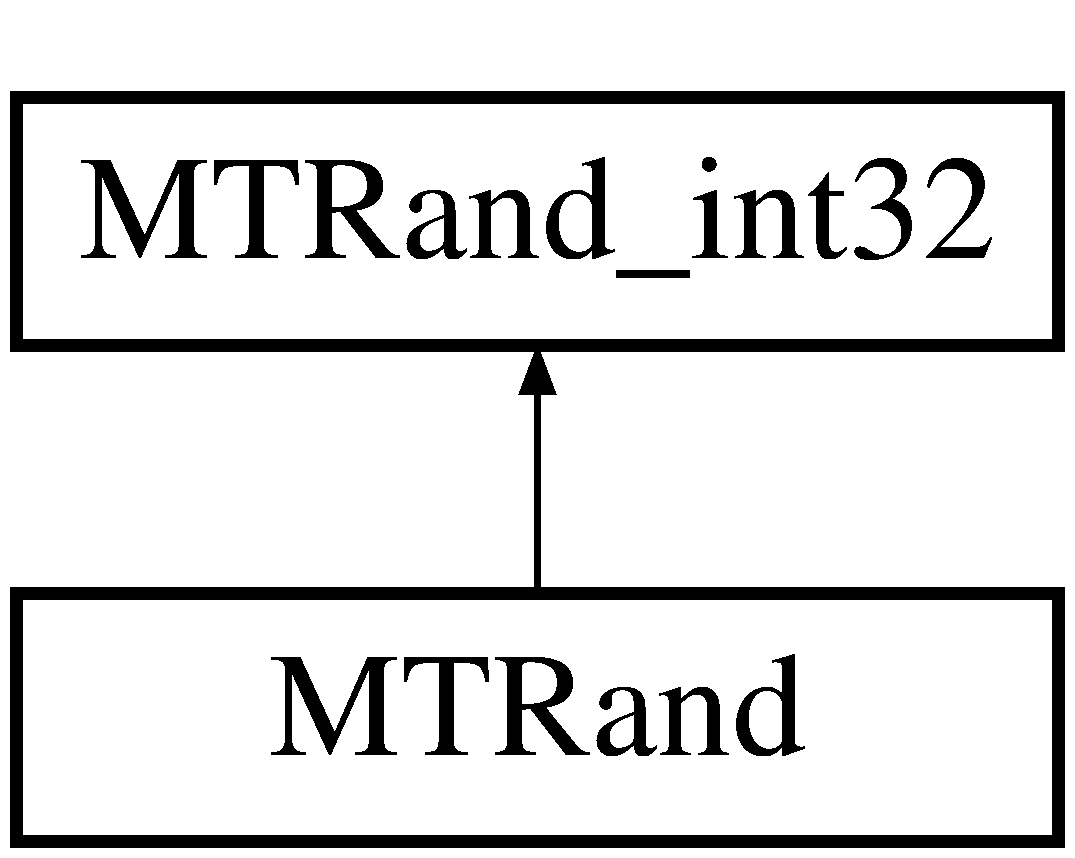
\includegraphics[height=2cm]{classMTRand}
\end{center}
\end{figure}
\subsection*{Public Member Functions}
\begin{CompactItemize}
\item 
{\bf MTRand} ()
\item 
{\bf MTRand} (unsigned long seed)
\item 
{\bf MTRand} (const unsigned long $\ast$seed, int size)
\item 
{\bf $\sim$MTRand} ()
\item 
double {\bf operator()} ()
\end{CompactItemize}


\subsection{Constructor \& Destructor Documentation}
\index{MTRand@{MTRand}!MTRand@{MTRand}}
\index{MTRand@{MTRand}!MTRand@{MTRand}}
\subsubsection{\setlength{\rightskip}{0pt plus 5cm}MTRand::MTRand ()\hspace{0.3cm}{\tt  [inline]}}\label{classMTRand_265dc65546e26073c0d5f8787b045a1d}


\index{MTRand@{MTRand}!MTRand@{MTRand}}
\index{MTRand@{MTRand}!MTRand@{MTRand}}
\subsubsection{\setlength{\rightskip}{0pt plus 5cm}MTRand::MTRand (unsigned long {\em seed})\hspace{0.3cm}{\tt  [inline]}}\label{classMTRand_2c88736896bcbdb54bcdd7a0026720d5}


\index{MTRand@{MTRand}!MTRand@{MTRand}}
\index{MTRand@{MTRand}!MTRand@{MTRand}}
\subsubsection{\setlength{\rightskip}{0pt plus 5cm}MTRand::MTRand (const unsigned long $\ast$ {\em seed}, int {\em size})\hspace{0.3cm}{\tt  [inline]}}\label{classMTRand_6075a3beacdfb8e4cf48d9fb56cc193a}


\index{MTRand@{MTRand}!$\sim$MTRand@{$\sim$MTRand}}
\index{$\sim$MTRand@{$\sim$MTRand}!MTRand@{MTRand}}
\subsubsection{\setlength{\rightskip}{0pt plus 5cm}MTRand::$\sim$MTRand ()\hspace{0.3cm}{\tt  [inline]}}\label{classMTRand_8c276546a41ae350dc9efc5e9c10a261}




\subsection{Member Function Documentation}
\index{MTRand@{MTRand}!operator()@{operator()}}
\index{operator()@{operator()}!MTRand@{MTRand}}
\subsubsection{\setlength{\rightskip}{0pt plus 5cm}double MTRand::operator() ()\hspace{0.3cm}{\tt  [inline]}}\label{classMTRand_bbb87a08d622d58fdee0eea4cb5471a0}




Reimplemented from {\bf MTRand\_\-int32} \doxyref{}{p.}{classMTRand__int32_d7fe22190d0411c6dac8e6f471633aa4}.

The documentation for this class was generated from the following file:\begin{CompactItemize}
\item 
/home/msneddon/eclipse/ganymede\_\-cpp/workspace/NFsim\_\-svn/src/NFutil/MTrand/{\bf mtrand.h}\end{CompactItemize}

\section{MTRand53 Class Reference}
\label{classMTRand53}\index{MTRand53@{MTRand53}}
{\tt \#include $<$mtrand.h$>$}

Inheritance diagram for MTRand53::\begin{figure}[H]
\begin{center}
\leavevmode
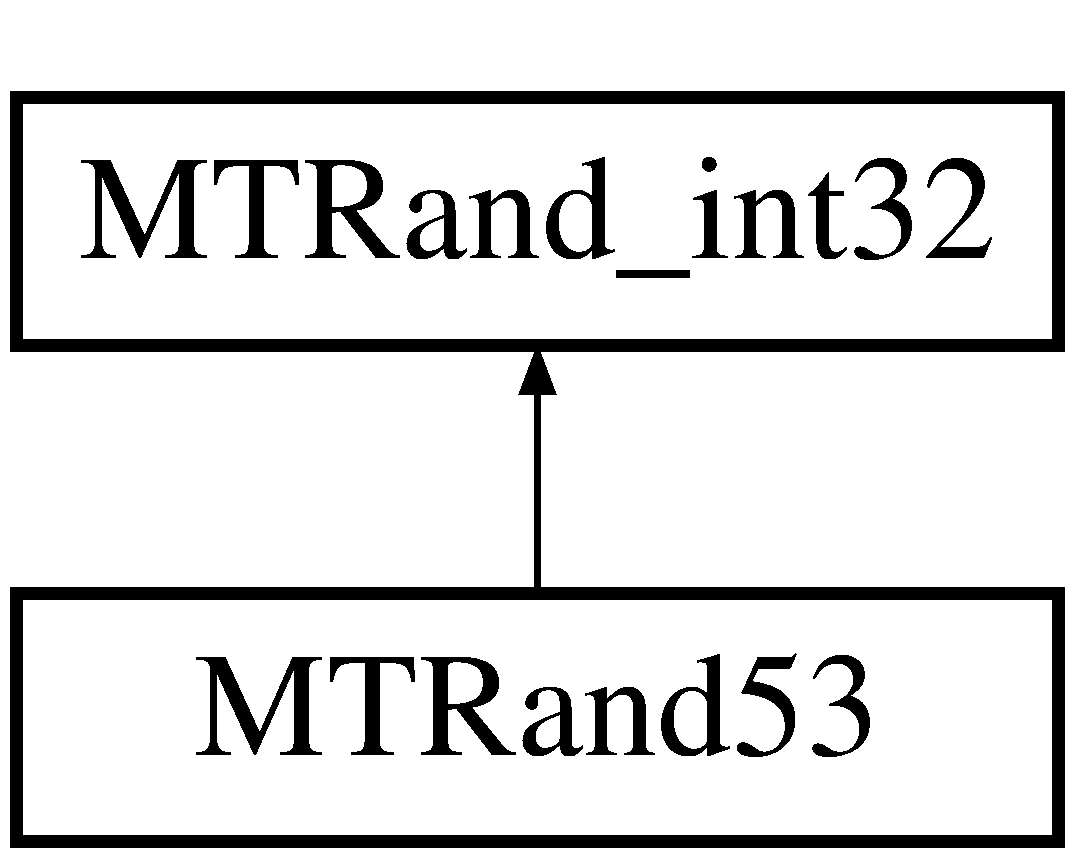
\includegraphics[height=2cm]{classMTRand53}
\end{center}
\end{figure}
\subsection*{Public Member Functions}
\begin{CompactItemize}
\item 
{\bf MTRand53} ()
\item 
{\bf MTRand53} (unsigned long seed)
\item 
{\bf MTRand53} (const unsigned long $\ast$seed, int size)
\item 
{\bf $\sim$MTRand53} ()
\item 
double {\bf operator()} ()
\end{CompactItemize}


\subsection{Constructor \& Destructor Documentation}
\index{MTRand53@{MTRand53}!MTRand53@{MTRand53}}
\index{MTRand53@{MTRand53}!MTRand53@{MTRand53}}
\subsubsection{\setlength{\rightskip}{0pt plus 5cm}MTRand53::MTRand53 ()\hspace{0.3cm}{\tt  [inline]}}\label{classMTRand53_24711c9e6e5ee72715f34515d1f1939a}


\index{MTRand53@{MTRand53}!MTRand53@{MTRand53}}
\index{MTRand53@{MTRand53}!MTRand53@{MTRand53}}
\subsubsection{\setlength{\rightskip}{0pt plus 5cm}MTRand53::MTRand53 (unsigned long {\em seed})\hspace{0.3cm}{\tt  [inline]}}\label{classMTRand53_d800887e15d4095f22facdb67f270c5e}


\index{MTRand53@{MTRand53}!MTRand53@{MTRand53}}
\index{MTRand53@{MTRand53}!MTRand53@{MTRand53}}
\subsubsection{\setlength{\rightskip}{0pt plus 5cm}MTRand53::MTRand53 (const unsigned long $\ast$ {\em seed}, int {\em size})\hspace{0.3cm}{\tt  [inline]}}\label{classMTRand53_c77b190d3ac27adea2d2c6c2ce2347c3}


\index{MTRand53@{MTRand53}!$\sim$MTRand53@{$\sim$MTRand53}}
\index{$\sim$MTRand53@{$\sim$MTRand53}!MTRand53@{MTRand53}}
\subsubsection{\setlength{\rightskip}{0pt plus 5cm}MTRand53::$\sim$MTRand53 ()\hspace{0.3cm}{\tt  [inline]}}\label{classMTRand53_947a6a7afd0c8a17612cda3faa705a75}




\subsection{Member Function Documentation}
\index{MTRand53@{MTRand53}!operator()@{operator()}}
\index{operator()@{operator()}!MTRand53@{MTRand53}}
\subsubsection{\setlength{\rightskip}{0pt plus 5cm}double MTRand53::operator() ()\hspace{0.3cm}{\tt  [inline]}}\label{classMTRand53_b6657cb5349f39bc4553d3a970458b45}




Reimplemented from {\bf MTRand\_\-int32} \doxyref{}{p.}{classMTRand__int32_d7fe22190d0411c6dac8e6f471633aa4}.

The documentation for this class was generated from the following file:\begin{CompactItemize}
\item 
/home/msneddon/eclipse/ganymede\_\-cpp/workspace/NFsim\_\-svn/src/NFutil/MTrand/{\bf mtrand.h}\end{CompactItemize}

\section{MTRand\_\-closed Class Reference}
\label{classMTRand__closed}\index{MTRand\_\-closed@{MTRand\_\-closed}}
{\tt \#include $<$mtrand.h$>$}

Inheritance diagram for MTRand\_\-closed::\begin{figure}[H]
\begin{center}
\leavevmode
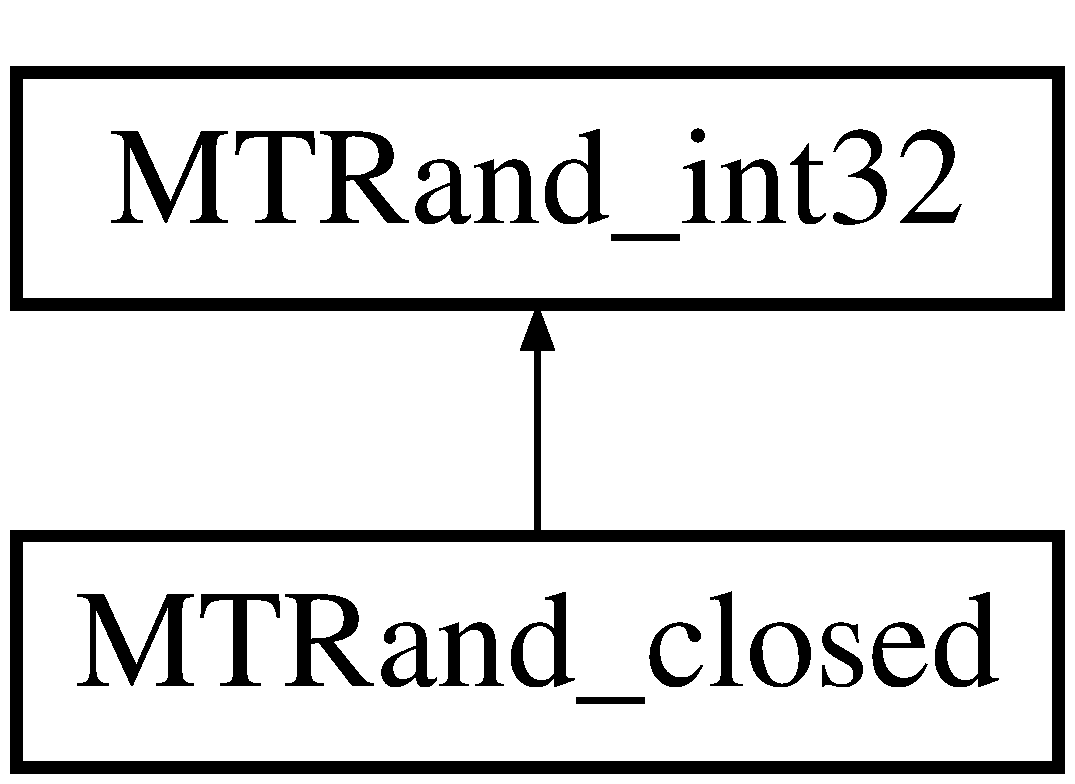
\includegraphics[height=2cm]{classMTRand__closed}
\end{center}
\end{figure}
\subsection*{Public Member Functions}
\begin{CompactItemize}
\item 
{\bf MTRand\_\-closed} ()
\item 
{\bf MTRand\_\-closed} (unsigned long seed)
\item 
{\bf MTRand\_\-closed} (const unsigned long $\ast$seed, int size)
\item 
{\bf $\sim$MTRand\_\-closed} ()
\item 
double {\bf operator()} ()
\end{CompactItemize}


\subsection{Constructor \& Destructor Documentation}
\index{MTRand\_\-closed@{MTRand\_\-closed}!MTRand\_\-closed@{MTRand\_\-closed}}
\index{MTRand\_\-closed@{MTRand\_\-closed}!MTRand_closed@{MTRand\_\-closed}}
\subsubsection{\setlength{\rightskip}{0pt plus 5cm}MTRand\_\-closed::MTRand\_\-closed ()\hspace{0.3cm}{\tt  [inline]}}\label{classMTRand__closed_09b3b21b3cb35d04f2b6c290a817b2e8}


\index{MTRand\_\-closed@{MTRand\_\-closed}!MTRand\_\-closed@{MTRand\_\-closed}}
\index{MTRand\_\-closed@{MTRand\_\-closed}!MTRand_closed@{MTRand\_\-closed}}
\subsubsection{\setlength{\rightskip}{0pt plus 5cm}MTRand\_\-closed::MTRand\_\-closed (unsigned long {\em seed})\hspace{0.3cm}{\tt  [inline]}}\label{classMTRand__closed_d5dc83250b16f22d4693a18b51816271}


\index{MTRand\_\-closed@{MTRand\_\-closed}!MTRand\_\-closed@{MTRand\_\-closed}}
\index{MTRand\_\-closed@{MTRand\_\-closed}!MTRand_closed@{MTRand\_\-closed}}
\subsubsection{\setlength{\rightskip}{0pt plus 5cm}MTRand\_\-closed::MTRand\_\-closed (const unsigned long $\ast$ {\em seed}, int {\em size})\hspace{0.3cm}{\tt  [inline]}}\label{classMTRand__closed_37e322f97253b7013823a267bcfe82d1}


\index{MTRand\_\-closed@{MTRand\_\-closed}!$\sim$MTRand\_\-closed@{$\sim$MTRand\_\-closed}}
\index{$\sim$MTRand\_\-closed@{$\sim$MTRand\_\-closed}!MTRand_closed@{MTRand\_\-closed}}
\subsubsection{\setlength{\rightskip}{0pt plus 5cm}MTRand\_\-closed::$\sim$MTRand\_\-closed ()\hspace{0.3cm}{\tt  [inline]}}\label{classMTRand__closed_46567ee841b5f54b305ac051ac837a8c}




\subsection{Member Function Documentation}
\index{MTRand\_\-closed@{MTRand\_\-closed}!operator()@{operator()}}
\index{operator()@{operator()}!MTRand_closed@{MTRand\_\-closed}}
\subsubsection{\setlength{\rightskip}{0pt plus 5cm}double MTRand\_\-closed::operator() ()\hspace{0.3cm}{\tt  [inline]}}\label{classMTRand__closed_d0c535263b63c95029523183f672f62d}




Reimplemented from {\bf MTRand\_\-int32} \doxyref{}{p.}{classMTRand__int32_d7fe22190d0411c6dac8e6f471633aa4}.

The documentation for this class was generated from the following file:\begin{CompactItemize}
\item 
/home/msneddon/eclipse/indigo/workspace/NFsim/src/NFutil/MTrand/{\bf mtrand.h}\end{CompactItemize}

\section{MTRand\_\-int32 Class Reference}
\label{classMTRand__int32}\index{MTRand\_\-int32@{MTRand\_\-int32}}
{\tt \#include $<$mtrand.h$>$}

Inheritance diagram for MTRand\_\-int32::\begin{figure}[H]
\begin{center}
\leavevmode
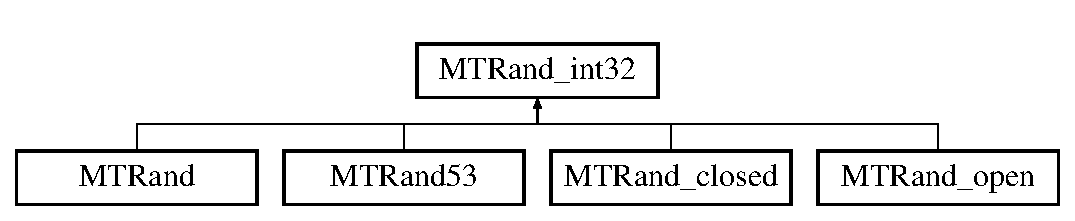
\includegraphics[height=2cm]{classMTRand__int32}
\end{center}
\end{figure}
\subsection*{Public Member Functions}
\begin{CompactItemize}
\item 
{\bf MTRand\_\-int32} ()
\item 
{\bf MTRand\_\-int32} (unsigned long s)
\item 
{\bf MTRand\_\-int32} (const unsigned long $\ast$array, int size)
\item 
void {\bf seed} (unsigned long)
\item 
void {\bf seed} (const unsigned long $\ast$, int size)
\item 
unsigned long {\bf operator()} ()
\item 
virtual {\bf $\sim$MTRand\_\-int32} ()
\end{CompactItemize}
\subsection*{Protected Member Functions}
\begin{CompactItemize}
\item 
unsigned long {\bf rand\_\-int32} ()
\end{CompactItemize}


\subsection{Constructor \& Destructor Documentation}
\index{MTRand\_\-int32@{MTRand\_\-int32}!MTRand\_\-int32@{MTRand\_\-int32}}
\index{MTRand\_\-int32@{MTRand\_\-int32}!MTRand_int32@{MTRand\_\-int32}}
\subsubsection{\setlength{\rightskip}{0pt plus 5cm}MTRand\_\-int32::MTRand\_\-int32 ()\hspace{0.3cm}{\tt  [inline]}}\label{classMTRand__int32_034f223c086f5368bd220b02f2cc12a8}


\index{MTRand\_\-int32@{MTRand\_\-int32}!MTRand\_\-int32@{MTRand\_\-int32}}
\index{MTRand\_\-int32@{MTRand\_\-int32}!MTRand_int32@{MTRand\_\-int32}}
\subsubsection{\setlength{\rightskip}{0pt plus 5cm}MTRand\_\-int32::MTRand\_\-int32 (unsigned long {\em s})\hspace{0.3cm}{\tt  [inline]}}\label{classMTRand__int32_d30f7c63a6f1fb3c3b76b8ce6ffa0206}


\index{MTRand\_\-int32@{MTRand\_\-int32}!MTRand\_\-int32@{MTRand\_\-int32}}
\index{MTRand\_\-int32@{MTRand\_\-int32}!MTRand_int32@{MTRand\_\-int32}}
\subsubsection{\setlength{\rightskip}{0pt plus 5cm}MTRand\_\-int32::MTRand\_\-int32 (const unsigned long $\ast$ {\em array}, int {\em size})\hspace{0.3cm}{\tt  [inline]}}\label{classMTRand__int32_19acddb3910a7282517b2ffc398b92b4}


\index{MTRand\_\-int32@{MTRand\_\-int32}!$\sim$MTRand\_\-int32@{$\sim$MTRand\_\-int32}}
\index{$\sim$MTRand\_\-int32@{$\sim$MTRand\_\-int32}!MTRand_int32@{MTRand\_\-int32}}
\subsubsection{\setlength{\rightskip}{0pt plus 5cm}virtual MTRand\_\-int32::$\sim$MTRand\_\-int32 ()\hspace{0.3cm}{\tt  [inline, virtual]}}\label{classMTRand__int32_364900abea0758d070ce89922159923a}




\subsection{Member Function Documentation}
\index{MTRand\_\-int32@{MTRand\_\-int32}!seed@{seed}}
\index{seed@{seed}!MTRand_int32@{MTRand\_\-int32}}
\subsubsection{\setlength{\rightskip}{0pt plus 5cm}void MTRand\_\-int32::seed (unsigned long {\em s})}\label{classMTRand__int32_0c57076fe30358e0700a7ce1baa0ea27}


\index{MTRand\_\-int32@{MTRand\_\-int32}!seed@{seed}}
\index{seed@{seed}!MTRand_int32@{MTRand\_\-int32}}
\subsubsection{\setlength{\rightskip}{0pt plus 5cm}void MTRand\_\-int32::seed (const unsigned long $\ast$ {\em array}, int {\em size})}\label{classMTRand__int32_3cabc1e3445716236a570ffd2f69686d}


\index{MTRand\_\-int32@{MTRand\_\-int32}!operator()@{operator()}}
\index{operator()@{operator()}!MTRand_int32@{MTRand\_\-int32}}
\subsubsection{\setlength{\rightskip}{0pt plus 5cm}unsigned long MTRand\_\-int32::operator() ()\hspace{0.3cm}{\tt  [inline]}}\label{classMTRand__int32_d7fe22190d0411c6dac8e6f471633aa4}




Reimplemented in {\bf MTRand} \doxyref{}{p.}{classMTRand_bbb87a08d622d58fdee0eea4cb5471a0}, {\bf MTRand\_\-closed} \doxyref{}{p.}{classMTRand__closed_d0c535263b63c95029523183f672f62d}, {\bf MTRand\_\-open} \doxyref{}{p.}{classMTRand__open_c408aa400ca59fc2afc888d88f98d807}, and {\bf MTRand53} \doxyref{}{p.}{classMTRand53_b6657cb5349f39bc4553d3a970458b45}.\index{MTRand\_\-int32@{MTRand\_\-int32}!rand\_\-int32@{rand\_\-int32}}
\index{rand\_\-int32@{rand\_\-int32}!MTRand_int32@{MTRand\_\-int32}}
\subsubsection{\setlength{\rightskip}{0pt plus 5cm}unsigned long MTRand\_\-int32::rand\_\-int32 ()\hspace{0.3cm}{\tt  [inline, protected]}}\label{classMTRand__int32_bacdfa346255baeac69d29bb57f29b22}




The documentation for this class was generated from the following files:\begin{CompactItemize}
\item 
/home/msneddon/eclipse/galileoSR1\_\-cpp/workspace/NFsim/src/NFutil/MTrand/{\bf mtrand.h}\item 
/home/msneddon/eclipse/galileoSR1\_\-cpp/workspace/NFsim/src/NFutil/MTrand/{\bf mtrand.cpp}\end{CompactItemize}

\section{MTRand\_\-open Class Reference}
\label{classMTRand__open}\index{MTRand\_\-open@{MTRand\_\-open}}
{\tt \#include $<$mtrand.h$>$}

Inheritance diagram for MTRand\_\-open::\begin{figure}[H]
\begin{center}
\leavevmode
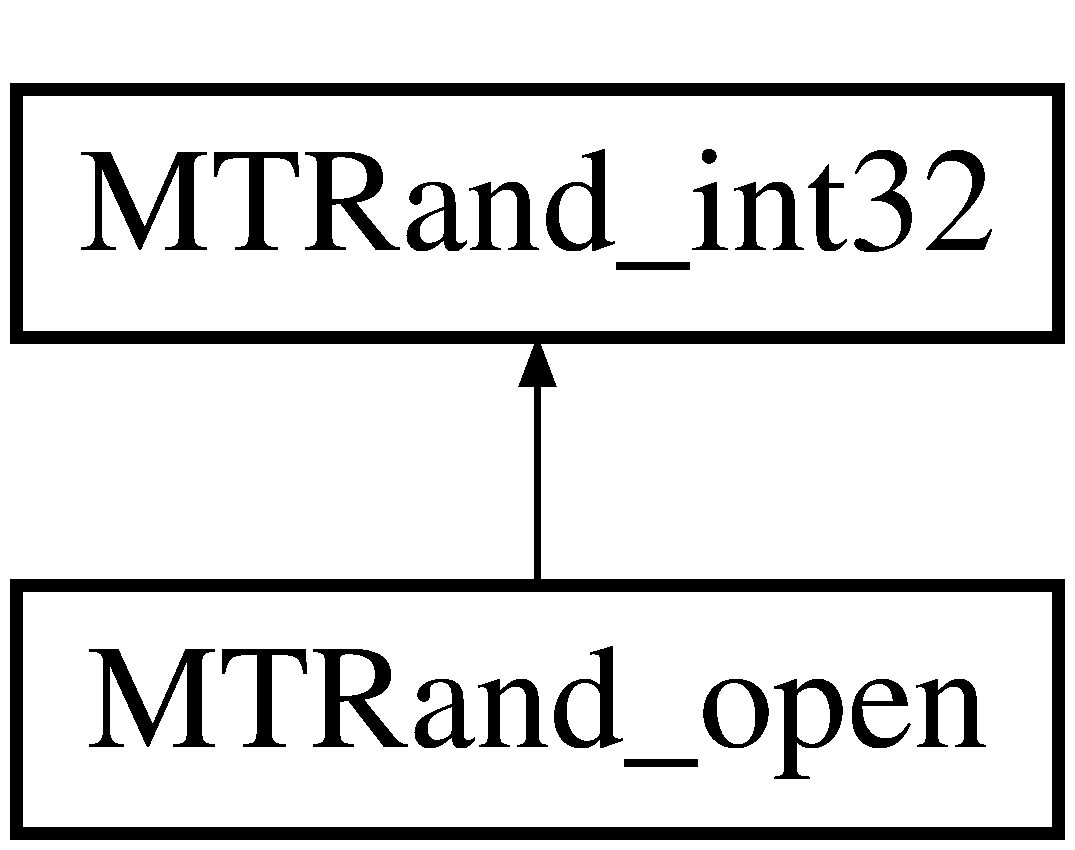
\includegraphics[height=2cm]{classMTRand__open}
\end{center}
\end{figure}
\subsection*{Public Member Functions}
\begin{CompactItemize}
\item 
{\bf MTRand\_\-open} ()
\item 
{\bf MTRand\_\-open} (unsigned long seed)
\item 
{\bf MTRand\_\-open} (const unsigned long $\ast$seed, int size)
\item 
{\bf $\sim$MTRand\_\-open} ()
\item 
double {\bf operator()} ()
\end{CompactItemize}


\subsection{Constructor \& Destructor Documentation}
\index{MTRand\_\-open@{MTRand\_\-open}!MTRand\_\-open@{MTRand\_\-open}}
\index{MTRand\_\-open@{MTRand\_\-open}!MTRand_open@{MTRand\_\-open}}
\subsubsection{\setlength{\rightskip}{0pt plus 5cm}MTRand\_\-open::MTRand\_\-open ()\hspace{0.3cm}{\tt  [inline]}}\label{classMTRand__open_58140b54564be39382da163954177389}


\index{MTRand\_\-open@{MTRand\_\-open}!MTRand\_\-open@{MTRand\_\-open}}
\index{MTRand\_\-open@{MTRand\_\-open}!MTRand_open@{MTRand\_\-open}}
\subsubsection{\setlength{\rightskip}{0pt plus 5cm}MTRand\_\-open::MTRand\_\-open (unsigned long {\em seed})\hspace{0.3cm}{\tt  [inline]}}\label{classMTRand__open_1f55ebc1052f5343f8d6e08a752ef957}


\index{MTRand\_\-open@{MTRand\_\-open}!MTRand\_\-open@{MTRand\_\-open}}
\index{MTRand\_\-open@{MTRand\_\-open}!MTRand_open@{MTRand\_\-open}}
\subsubsection{\setlength{\rightskip}{0pt plus 5cm}MTRand\_\-open::MTRand\_\-open (const unsigned long $\ast$ {\em seed}, int {\em size})\hspace{0.3cm}{\tt  [inline]}}\label{classMTRand__open_0216992f4dfa5acf22ee8c585eeac488}


\index{MTRand\_\-open@{MTRand\_\-open}!$\sim$MTRand\_\-open@{$\sim$MTRand\_\-open}}
\index{$\sim$MTRand\_\-open@{$\sim$MTRand\_\-open}!MTRand_open@{MTRand\_\-open}}
\subsubsection{\setlength{\rightskip}{0pt plus 5cm}MTRand\_\-open::$\sim$MTRand\_\-open ()\hspace{0.3cm}{\tt  [inline]}}\label{classMTRand__open_4f4774b5d9b79972dedaec984b248581}




\subsection{Member Function Documentation}
\index{MTRand\_\-open@{MTRand\_\-open}!operator()@{operator()}}
\index{operator()@{operator()}!MTRand_open@{MTRand\_\-open}}
\subsubsection{\setlength{\rightskip}{0pt plus 5cm}double MTRand\_\-open::operator() ()\hspace{0.3cm}{\tt  [inline]}}\label{classMTRand__open_c408aa400ca59fc2afc888d88f98d807}




Reimplemented from {\bf MTRand\_\-int32} \doxyref{}{p.}{classMTRand__int32_d7fe22190d0411c6dac8e6f471633aa4}.

The documentation for this class was generated from the following file:\begin{CompactItemize}
\item 
/home/msneddon/eclipse/ganymede\_\-cpp/workspace/NFsim\_\-svn/src/NFutil/MTrand/{\bf mtrand.h}\end{CompactItemize}

\section{NFcore::Observable Class Reference}
\label{classNFcore_1_1Observable}\index{NFcore::Observable@{NFcore::Observable}}
{\tt \#include $<$NFcore.hh$>$}



\subsection{Detailed Description}
Tracks the counts of predefined observables in the simulation. 

Observables keep track of the counts of specific \doxyref{Molecule}{p.}{classNFcore_1_1Molecule} configurations in the system. Observables use TemplateMolecules to determine if a \doxyref{Molecule}{p.}{classNFcore_1_1Molecule} configuration should be counted as an \doxyref{Observable}{p.}{classNFcore_1_1Observable}. Users have the choice of computing Observables on the fly so that they are incrementally updated after each event or recomputing all Observables before each output step. \begin{Desc}
\item[Author:]Michael Sneddon \end{Desc}
\subsection*{Public Member Functions}
\begin{CompactItemize}
\item 
{\bf Observable} (string {\bf aliasName}, {\bf TemplateMolecule} $\ast${\bf templateMolecule})
\item 
{\bf $\sim$Observable} ()
\item 
bool {\bf isObservable} ({\bf Molecule} $\ast$m) const 
\item 
void {\bf add} ()
\item 
void {\bf subtract} ()
\item 
void {\bf clear} ()
\item 
void {\bf straightAdd} ()
\item 
unsigned long int {\bf getCount} () const 
\item 
string {\bf getAliasName} () const 
\item 
void {\bf addReferenceToMyself} (mu::Parser $\ast$p)
\item 
void {\bf addDependentRxn} ({\bf ReactionClass} $\ast$r)
\item 
{\bf TemplateMolecule} $\ast$ {\bf getTemplateMolecule} () const 
\end{CompactItemize}
\subsection*{Protected Attributes}
\begin{CompactItemize}
\item 
string {\bf aliasName}
\item 
{\bf TemplateMolecule} $\ast$ {\bf templateMolecule}
\item 
double {\bf count}
\item 
vector$<$ {\bf ReactionClass} $\ast$ $>$ {\bf dependentRxns}
\item 
vector$<$ {\bf ReactionClass} $\ast$ $>$::iterator {\bf rxnIter}
\end{CompactItemize}


\subsection{Constructor \& Destructor Documentation}
\index{NFcore::Observable@{NFcore::Observable}!Observable@{Observable}}
\index{Observable@{Observable}!NFcore::Observable@{NFcore::Observable}}
\subsubsection{\setlength{\rightskip}{0pt plus 5cm}Observable::Observable (string {\em aliasName}, {\bf TemplateMolecule} $\ast$ {\em templateMolecule})}\label{classNFcore_1_1Observable_df141ff9a226f066afa6f0b6ec3307ee}


Constructor that creates a basic \doxyref{Observable}{p.}{classNFcore_1_1Observable} which monitors the given \doxyref{TemplateMolecule}{p.}{classNFcore_1_1TemplateMolecule} and can be referenced via the alias name \index{NFcore::Observable@{NFcore::Observable}!$\sim$Observable@{$\sim$Observable}}
\index{$\sim$Observable@{$\sim$Observable}!NFcore::Observable@{NFcore::Observable}}
\subsubsection{\setlength{\rightskip}{0pt plus 5cm}Observable::$\sim$Observable ()}\label{classNFcore_1_1Observable_89d963584ab7007ee9412ebdc859f5f2}


Deconstructor that doesn't do too much. It doesn't free the memory associated with the \doxyref{TemplateMolecule}{p.}{classNFcore_1_1TemplateMolecule} because the \doxyref{MoleculeType}{p.}{classNFcore_1_1MoleculeType} class handles that. 

\subsection{Member Function Documentation}
\index{NFcore::Observable@{NFcore::Observable}!isObservable@{isObservable}}
\index{isObservable@{isObservable}!NFcore::Observable@{NFcore::Observable}}
\subsubsection{\setlength{\rightskip}{0pt plus 5cm}bool Observable::isObservable ({\bf Molecule} $\ast$ {\em m}) const}\label{classNFcore_1_1Observable_cf5f192d663b138ce780f86fa5ddc557}


\index{NFcore::Observable@{NFcore::Observable}!add@{add}}
\index{add@{add}!NFcore::Observable@{NFcore::Observable}}
\subsubsection{\setlength{\rightskip}{0pt plus 5cm}void Observable::add ()}\label{classNFcore_1_1Observable_955408d15da68cb8c420d0c62765edc0}


\index{NFcore::Observable@{NFcore::Observable}!subtract@{subtract}}
\index{subtract@{subtract}!NFcore::Observable@{NFcore::Observable}}
\subsubsection{\setlength{\rightskip}{0pt plus 5cm}void Observable::subtract ()}\label{classNFcore_1_1Observable_89bb17beddaec3e99b5fc11898d12a2a}


\index{NFcore::Observable@{NFcore::Observable}!clear@{clear}}
\index{clear@{clear}!NFcore::Observable@{NFcore::Observable}}
\subsubsection{\setlength{\rightskip}{0pt plus 5cm}void NFcore::Observable::clear ()\hspace{0.3cm}{\tt  [inline]}}\label{classNFcore_1_1Observable_2413c48e53ed66c2a5c79999cc3825ed}


\index{NFcore::Observable@{NFcore::Observable}!straightAdd@{straightAdd}}
\index{straightAdd@{straightAdd}!NFcore::Observable@{NFcore::Observable}}
\subsubsection{\setlength{\rightskip}{0pt plus 5cm}void NFcore::Observable::straightAdd ()\hspace{0.3cm}{\tt  [inline]}}\label{classNFcore_1_1Observable_f35f24cc8d818349c2ebe3c326c54048}


\index{NFcore::Observable@{NFcore::Observable}!getCount@{getCount}}
\index{getCount@{getCount}!NFcore::Observable@{NFcore::Observable}}
\subsubsection{\setlength{\rightskip}{0pt plus 5cm}unsigned long int NFcore::Observable::getCount () const\hspace{0.3cm}{\tt  [inline]}}\label{classNFcore_1_1Observable_4e4524075d723eaf9dcfd7c150734996}


\index{NFcore::Observable@{NFcore::Observable}!getAliasName@{getAliasName}}
\index{getAliasName@{getAliasName}!NFcore::Observable@{NFcore::Observable}}
\subsubsection{\setlength{\rightskip}{0pt plus 5cm}string NFcore::Observable::getAliasName () const\hspace{0.3cm}{\tt  [inline]}}\label{classNFcore_1_1Observable_34e399e7cbb6c511cf849e921e21d352}


\index{NFcore::Observable@{NFcore::Observable}!addReferenceToMyself@{addReferenceToMyself}}
\index{addReferenceToMyself@{addReferenceToMyself}!NFcore::Observable@{NFcore::Observable}}
\subsubsection{\setlength{\rightskip}{0pt plus 5cm}void Observable::addReferenceToMyself (mu::Parser $\ast$ {\em p})}\label{classNFcore_1_1Observable_3210dd6179e6cfb124d012fa22f1e5c4}


\index{NFcore::Observable@{NFcore::Observable}!addDependentRxn@{addDependentRxn}}
\index{addDependentRxn@{addDependentRxn}!NFcore::Observable@{NFcore::Observable}}
\subsubsection{\setlength{\rightskip}{0pt plus 5cm}void Observable::addDependentRxn ({\bf ReactionClass} $\ast$ {\em r})}\label{classNFcore_1_1Observable_7f982704d5ae35afc68513e331bdb88c}


\index{NFcore::Observable@{NFcore::Observable}!getTemplateMolecule@{getTemplateMolecule}}
\index{getTemplateMolecule@{getTemplateMolecule}!NFcore::Observable@{NFcore::Observable}}
\subsubsection{\setlength{\rightskip}{0pt plus 5cm}{\bf TemplateMolecule}$\ast$ NFcore::Observable::getTemplateMolecule () const\hspace{0.3cm}{\tt  [inline]}}\label{classNFcore_1_1Observable_9e8ce13e756d2501bc3ae799cf012821}




\subsection{Member Data Documentation}
\index{NFcore::Observable@{NFcore::Observable}!aliasName@{aliasName}}
\index{aliasName@{aliasName}!NFcore::Observable@{NFcore::Observable}}
\subsubsection{\setlength{\rightskip}{0pt plus 5cm}string {\bf NFcore::Observable::aliasName}\hspace{0.3cm}{\tt  [protected]}}\label{classNFcore_1_1Observable_5696b7a468ef66abb74459dac4efc9f1}


\index{NFcore::Observable@{NFcore::Observable}!templateMolecule@{templateMolecule}}
\index{templateMolecule@{templateMolecule}!NFcore::Observable@{NFcore::Observable}}
\subsubsection{\setlength{\rightskip}{0pt plus 5cm}{\bf TemplateMolecule}$\ast$ {\bf NFcore::Observable::templateMolecule}\hspace{0.3cm}{\tt  [protected]}}\label{classNFcore_1_1Observable_f5a8f61d8c752499ec9630aa4ed625ca}


\index{NFcore::Observable@{NFcore::Observable}!count@{count}}
\index{count@{count}!NFcore::Observable@{NFcore::Observable}}
\subsubsection{\setlength{\rightskip}{0pt plus 5cm}double {\bf NFcore::Observable::count}\hspace{0.3cm}{\tt  [protected]}}\label{classNFcore_1_1Observable_a71c7a1b37fe6a58dd93647e4e2600b0}


\index{NFcore::Observable@{NFcore::Observable}!dependentRxns@{dependentRxns}}
\index{dependentRxns@{dependentRxns}!NFcore::Observable@{NFcore::Observable}}
\subsubsection{\setlength{\rightskip}{0pt plus 5cm}vector$<${\bf ReactionClass} $\ast$$>$ {\bf NFcore::Observable::dependentRxns}\hspace{0.3cm}{\tt  [protected]}}\label{classNFcore_1_1Observable_31559398cafc369fa565bb1e9d2c059a}


\index{NFcore::Observable@{NFcore::Observable}!rxnIter@{rxnIter}}
\index{rxnIter@{rxnIter}!NFcore::Observable@{NFcore::Observable}}
\subsubsection{\setlength{\rightskip}{0pt plus 5cm}vector$<${\bf ReactionClass} $\ast$$>$::iterator {\bf NFcore::Observable::rxnIter}\hspace{0.3cm}{\tt  [protected]}}\label{classNFcore_1_1Observable_0dc6cd3858aab9b1dc4852c30571b269}




The documentation for this class was generated from the following files:\begin{CompactItemize}
\item 
/home/msneddon/eclipse/ganymede\_\-cpp/workspace/NFsim\_\-svn/src/NFcore/{\bf NFcore.hh}\item 
/home/msneddon/eclipse/ganymede\_\-cpp/workspace/NFsim\_\-svn/src/NFcore/{\bf observable.cpp}\end{CompactItemize}

\section{NFcore::Outputter Class Reference}
\label{classNFcore_1_1Outputter}\index{NFcore::Outputter@{NFcore::Outputter}}
{\tt \#include $<$NFoutput.hh$>$}

\subsection*{Public Member Functions}
\begin{CompactItemize}
\item 
{\bf Outputter} (string {\bf filename}, {\bf System} $\ast${\bf s})
\item 
virtual {\bf $\sim$Outputter} ()
\item 
virtual void {\bf output} ()=0
\item 
virtual void {\bf outputHeader} ()=0
\item 
virtual void {\bf tryToDump} (double simTime)=0
\end{CompactItemize}
\subsection*{Protected Attributes}
\begin{CompactItemize}
\item 
string {\bf filename}
\item 
{\bf System} $\ast$ {\bf s}
\item 
ofstream {\bf outputFileStream}
\end{CompactItemize}


\subsection{Constructor \& Destructor Documentation}
\index{NFcore::Outputter@{NFcore::Outputter}!Outputter@{Outputter}}
\index{Outputter@{Outputter}!NFcore::Outputter@{NFcore::Outputter}}
\subsubsection{\setlength{\rightskip}{0pt plus 5cm}Outputter::Outputter (string {\em filename}, {\bf System} $\ast$ {\em s})}\label{classNFcore_1_1Outputter_92551e7d729d3fba3f52600c2d23a7f8}


\index{NFcore::Outputter@{NFcore::Outputter}!$\sim$Outputter@{$\sim$Outputter}}
\index{$\sim$Outputter@{$\sim$Outputter}!NFcore::Outputter@{NFcore::Outputter}}
\subsubsection{\setlength{\rightskip}{0pt plus 5cm}Outputter::$\sim$Outputter ()\hspace{0.3cm}{\tt  [virtual]}}\label{classNFcore_1_1Outputter_d2fa668dffa24b574f6edc69062cf06e}




\subsection{Member Function Documentation}
\index{NFcore::Outputter@{NFcore::Outputter}!output@{output}}
\index{output@{output}!NFcore::Outputter@{NFcore::Outputter}}
\subsubsection{\setlength{\rightskip}{0pt plus 5cm}virtual void NFcore::Outputter::output ()\hspace{0.3cm}{\tt  [pure virtual]}}\label{classNFcore_1_1Outputter_fa0b98db6598c1d00b143b61f0c5c575}


\index{NFcore::Outputter@{NFcore::Outputter}!outputHeader@{outputHeader}}
\index{outputHeader@{outputHeader}!NFcore::Outputter@{NFcore::Outputter}}
\subsubsection{\setlength{\rightskip}{0pt plus 5cm}virtual void NFcore::Outputter::outputHeader ()\hspace{0.3cm}{\tt  [pure virtual]}}\label{classNFcore_1_1Outputter_14be13a01fc8c5c515bf4ddb8b721e3c}


\index{NFcore::Outputter@{NFcore::Outputter}!tryToDump@{tryToDump}}
\index{tryToDump@{tryToDump}!NFcore::Outputter@{NFcore::Outputter}}
\subsubsection{\setlength{\rightskip}{0pt plus 5cm}virtual void NFcore::Outputter::tryToDump (double {\em simTime})\hspace{0.3cm}{\tt  [pure virtual]}}\label{classNFcore_1_1Outputter_f6476687694630364712b462afea04e6}




\subsection{Member Data Documentation}
\index{NFcore::Outputter@{NFcore::Outputter}!filename@{filename}}
\index{filename@{filename}!NFcore::Outputter@{NFcore::Outputter}}
\subsubsection{\setlength{\rightskip}{0pt plus 5cm}string {\bf NFcore::Outputter::filename}\hspace{0.3cm}{\tt  [protected]}}\label{classNFcore_1_1Outputter_150c6ee5c2eb1f61eaef24139c05e4ed}


\index{NFcore::Outputter@{NFcore::Outputter}!s@{s}}
\index{s@{s}!NFcore::Outputter@{NFcore::Outputter}}
\subsubsection{\setlength{\rightskip}{0pt plus 5cm}{\bf System}$\ast$ {\bf NFcore::Outputter::s}\hspace{0.3cm}{\tt  [protected]}}\label{classNFcore_1_1Outputter_c63f98e10701598bf2dc79b0c76d2447}


\index{NFcore::Outputter@{NFcore::Outputter}!outputFileStream@{outputFileStream}}
\index{outputFileStream@{outputFileStream}!NFcore::Outputter@{NFcore::Outputter}}
\subsubsection{\setlength{\rightskip}{0pt plus 5cm}ofstream {\bf NFcore::Outputter::outputFileStream}\hspace{0.3cm}{\tt  [protected]}}\label{classNFcore_1_1Outputter_01b52e6b6164df23aac52809fb4d6ae6}




The documentation for this class was generated from the following files:\begin{CompactItemize}
\item 
/home/msneddon/eclipse/galileoSR1\_\-cpp/workspace/NFsim/src/NFoutput/{\bf NFoutput.hh}\item 
/home/msneddon/eclipse/galileoSR1\_\-cpp/workspace/NFsim/src/NFoutput/{\bf NFoutput.cpp}\end{CompactItemize}

\section{NFcore::ReactantList Class Reference}
\label{classNFcore_1_1ReactantList}\index{NFcore::ReactantList@{NFcore::ReactantList}}
{\tt \#include $<$reactantList.hh$>$}

Inheritance diagram for NFcore::ReactantList::\begin{figure}[H]
\begin{center}
\leavevmode
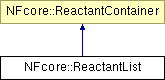
\includegraphics[height=2cm]{classNFcore_1_1ReactantList}
\end{center}
\end{figure}


\subsection{Detailed Description}
Maintains a list of MappingSets needed by \doxyref{ReactionClass}{p.}{classNFcore_1_1ReactionClass}. 

This is essentially a specialized vector implementation that allows a \doxyref{ReactionClass}{p.}{classNFcore_1_1ReactionClass} to easily keep track of all the \doxyref{MappingSet}{p.}{classNFcore_1_1MappingSet} objects that can be involved in the reaction. All \doxyref{MappingSet}{p.}{classNFcore_1_1MappingSet} objects stored in this class are created once and reused throughout the course of the simulation. This prevents new \doxyref{MappingSet}{p.}{classNFcore_1_1MappingSet} objects to be created and destroyed. This class has the ability to automatically expand its capacity when extra mappings are needed, so there is no need for the user to manage these details. This class allows for constant time removal, insertion, and random selection of MappingSets, while std::vector requires linear time removal. We gain this speedup because the ordering of the list is unimportant. To use this class, call the pushNextAvailableMappingSet to get a pointer to the available \doxyref{MappingSet}{p.}{classNFcore_1_1MappingSet}. Pass this \doxyref{MappingSet}{p.}{classNFcore_1_1MappingSet} to a \doxyref{TemplateMolecule}{p.}{classNFcore_1_1TemplateMolecule} to actually map it onto molecules. If you don't end up using this \doxyref{MappingSet}{p.}{classNFcore_1_1MappingSet}, call popLastMappingSet immediately. To remove MappingSets, call removeMappingSet with the ID of the \doxyref{MappingSet}{p.}{classNFcore_1_1MappingSet} you want to remove. You can get this Id from the \doxyref{MappingSet}{p.}{classNFcore_1_1MappingSet} object and \doxyref{Molecule}{p.}{classNFcore_1_1Molecule} objects also keep a vector of the \doxyref{MappingSet}{p.}{classNFcore_1_1MappingSet} objects that point to it. \begin{Desc}
\item[Author:]Michael Sneddon \end{Desc}
\subsection*{Public Member Functions}
\begin{CompactItemize}
\item 
{\bf ReactantList} (unsigned int {\bf reactantIndex}, {\bf TransformationSet} $\ast${\bf ts}, unsigned int init\_\-capacity)
\item 
virtual {\bf $\sim$ReactantList} ()
\item 
virtual int {\bf size} () const 
\item 
virtual {\bf MappingSet} $\ast$ {\bf pushNextAvailableMappingSet} ()
\item 
virtual void {\bf popLastMappingSet} ()
\item 
virtual void {\bf removeMappingSet} (unsigned int mappingSetId)
\item 
void {\bf pickRandom} ({\bf MappingSet} $\ast$\&ms)
\item 
virtual {\bf MappingSet} $\ast$ {\bf getMappingSet} (unsigned int mappingSetId) const 
\item 
virtual void {\bf printDetails} () const 
\end{CompactItemize}
\subsection*{Protected Attributes}
\begin{CompactItemize}
\item 
int {\bf n\_\-mappingSets}
\item 
int {\bf capacity}
\item 
{\bf TransformationSet} $\ast$ {\bf ts}
\item 
unsigned int {\bf reactantIndex}
\item 
unsigned int $\ast$ {\bf msPositionMap}
\item 
{\bf MappingSet} $\ast$$\ast$ {\bf mappingSets}
\end{CompactItemize}


\subsection{Constructor \& Destructor Documentation}
\index{NFcore::ReactantList@{NFcore::ReactantList}!ReactantList@{ReactantList}}
\index{ReactantList@{ReactantList}!NFcore::ReactantList@{NFcore::ReactantList}}
\subsubsection{\setlength{\rightskip}{0pt plus 5cm}ReactantList::ReactantList (unsigned int {\em reactantIndex}, {\bf TransformationSet} $\ast$ {\em ts}, unsigned int {\em init\_\-capacity} = {\tt 50})}\label{classNFcore_1_1ReactantList_6954011db54afca7613feac19f56e88a}


Creates a new empty \doxyref{ReactantList}{p.}{classNFcore_1_1ReactantList} with the given initial capacity (default is 50). This capacity should roughly be set to the number of mappings you expect this list to have. A reactantList must also be told what its reactionIndex is in the reaction and the \doxyref{TransformationSet}{p.}{classNFcore_1_1TransformationSet} of the reaction so that it can populate itself with MappingSets. \index{NFcore::ReactantList@{NFcore::ReactantList}!$\sim$ReactantList@{$\sim$ReactantList}}
\index{$\sim$ReactantList@{$\sim$ReactantList}!NFcore::ReactantList@{NFcore::ReactantList}}
\subsubsection{\setlength{\rightskip}{0pt plus 5cm}ReactantList::$\sim$ReactantList ()\hspace{0.3cm}{\tt  [virtual]}}\label{classNFcore_1_1ReactantList_69a80ae14aeb910930010c6e31e5943d}


Deconstructor that deletes all mappingSets associated with this list. 

\subsection{Member Function Documentation}
\index{NFcore::ReactantList@{NFcore::ReactantList}!size@{size}}
\index{size@{size}!NFcore::ReactantList@{NFcore::ReactantList}}
\subsubsection{\setlength{\rightskip}{0pt plus 5cm}virtual int NFcore::ReactantList::size () const\hspace{0.3cm}{\tt  [inline, virtual]}}\label{classNFcore_1_1ReactantList_f7ee7d25b15ee7adb71714c4f8cc5a0f}


Returns the number of mappingSets that have been added to this list 

Implements {\bf NFcore::ReactantContainer} \doxyref{}{p.}{classNFcore_1_1ReactantContainer_5c8282ceba6fcdf04ea4708a9ec5056a}.\index{NFcore::ReactantList@{NFcore::ReactantList}!pushNextAvailableMappingSet@{pushNextAvailableMappingSet}}
\index{pushNextAvailableMappingSet@{pushNextAvailableMappingSet}!NFcore::ReactantList@{NFcore::ReactantList}}
\subsubsection{\setlength{\rightskip}{0pt plus 5cm}{\bf MappingSet} $\ast$ ReactantList::pushNextAvailableMappingSet ()\hspace{0.3cm}{\tt  [virtual]}}\label{classNFcore_1_1ReactantList_cbd9b70dc5bec6a90afdff65e708bdbb}


Adds a new \doxyref{MappingSet}{p.}{classNFcore_1_1MappingSet} to this list and returns a pointer to the new mapping set for you to map (usually by comparing to some template molecule). Warning: even if you don't use this mapping set, it will be counted until you pop it! (see \doxyref{popLastMappingSet()}{p.}{classNFcore_1_1ReactantList_733d6d8d54398b5a5615f1f8f597b70f}). 

Implements {\bf NFcore::ReactantContainer} \doxyref{}{p.}{classNFcore_1_1ReactantContainer_e49f41bfe7c16fa1961da77e3924f7a6}.\index{NFcore::ReactantList@{NFcore::ReactantList}!popLastMappingSet@{popLastMappingSet}}
\index{popLastMappingSet@{popLastMappingSet}!NFcore::ReactantList@{NFcore::ReactantList}}
\subsubsection{\setlength{\rightskip}{0pt plus 5cm}void ReactantList::popLastMappingSet ()\hspace{0.3cm}{\tt  [virtual]}}\label{classNFcore_1_1ReactantList_733d6d8d54398b5a5615f1f8f597b70f}


Removes the very last mappingSet that was added to the list. 

Implements {\bf NFcore::ReactantContainer} \doxyref{}{p.}{classNFcore_1_1ReactantContainer_ea26d24f00e2632bd8c68210c0405293}.\index{NFcore::ReactantList@{NFcore::ReactantList}!removeMappingSet@{removeMappingSet}}
\index{removeMappingSet@{removeMappingSet}!NFcore::ReactantList@{NFcore::ReactantList}}
\subsubsection{\setlength{\rightskip}{0pt plus 5cm}void ReactantList::removeMappingSet (unsigned int {\em mappingSetId})\hspace{0.3cm}{\tt  [virtual]}}\label{classNFcore_1_1ReactantList_eff0073ca4bcda7cdd601fb78719caac}


Removes the mapping set with the specified mappingSetId. Be careful here: make sure the mapping set is actually on the list before trying to remove or else this will give you an error! 

Implements {\bf NFcore::ReactantContainer} \doxyref{}{p.}{classNFcore_1_1ReactantContainer_109cc95b0cba4b0f6b122953009d7be9}.\index{NFcore::ReactantList@{NFcore::ReactantList}!pickRandom@{pickRandom}}
\index{pickRandom@{pickRandom}!NFcore::ReactantList@{NFcore::ReactantList}}
\subsubsection{\setlength{\rightskip}{0pt plus 5cm}void ReactantList::pickRandom ({\bf MappingSet} $\ast$\& {\em ms})}\label{classNFcore_1_1ReactantList_fe1c91c30e5096eaebf6d3bd12ee824e}


Randomly selects a \doxyref{MappingSet}{p.}{classNFcore_1_1MappingSet} from the list of available MappingSets. \index{NFcore::ReactantList@{NFcore::ReactantList}!getMappingSet@{getMappingSet}}
\index{getMappingSet@{getMappingSet}!NFcore::ReactantList@{NFcore::ReactantList}}
\subsubsection{\setlength{\rightskip}{0pt plus 5cm}{\bf MappingSet} $\ast$ ReactantList::getMappingSet (unsigned int {\em mappingSetId}) const\hspace{0.3cm}{\tt  [virtual]}}\label{classNFcore_1_1ReactantList_9ce2c8a0c49cf0f40a5057cd311907ce}




Implements {\bf NFcore::ReactantContainer} \doxyref{}{p.}{classNFcore_1_1ReactantContainer_ed1f09a5f7224d2084ad1a487e36f189}.\index{NFcore::ReactantList@{NFcore::ReactantList}!printDetails@{printDetails}}
\index{printDetails@{printDetails}!NFcore::ReactantList@{NFcore::ReactantList}}
\subsubsection{\setlength{\rightskip}{0pt plus 5cm}void ReactantList::printDetails () const\hspace{0.3cm}{\tt  [virtual]}}\label{classNFcore_1_1ReactantList_8b9152df8b57fdc9e80e240a20525d5d}


Outputs basic details about this list - used only for debugging. 

Implements {\bf NFcore::ReactantContainer} \doxyref{}{p.}{classNFcore_1_1ReactantContainer_305122520e4c2b2fed2201b0bd307b76}.

\subsection{Member Data Documentation}
\index{NFcore::ReactantList@{NFcore::ReactantList}!n\_\-mappingSets@{n\_\-mappingSets}}
\index{n\_\-mappingSets@{n\_\-mappingSets}!NFcore::ReactantList@{NFcore::ReactantList}}
\subsubsection{\setlength{\rightskip}{0pt plus 5cm}int {\bf NFcore::ReactantList::n\_\-mappingSets}\hspace{0.3cm}{\tt  [protected]}}\label{classNFcore_1_1ReactantList_7425bc756e19906c0b021ac68ea476b5}


Maintains the number of mappingSets on this list \index{NFcore::ReactantList@{NFcore::ReactantList}!capacity@{capacity}}
\index{capacity@{capacity}!NFcore::ReactantList@{NFcore::ReactantList}}
\subsubsection{\setlength{\rightskip}{0pt plus 5cm}int {\bf NFcore::ReactantList::capacity}\hspace{0.3cm}{\tt  [protected]}}\label{classNFcore_1_1ReactantList_f4c404494ed0c305aebf943d477ac72e}


The total capacity that this list can hold \index{NFcore::ReactantList@{NFcore::ReactantList}!ts@{ts}}
\index{ts@{ts}!NFcore::ReactantList@{NFcore::ReactantList}}
\subsubsection{\setlength{\rightskip}{0pt plus 5cm}{\bf TransformationSet}$\ast$ {\bf NFcore::ReactantList::ts}\hspace{0.3cm}{\tt  [protected]}}\label{classNFcore_1_1ReactantList_96f0caa1c27c9349289c192f9e76605e}


The transformation set of the \doxyref{ReactionClass}{p.}{classNFcore_1_1ReactionClass} that owns this list \index{NFcore::ReactantList@{NFcore::ReactantList}!reactantIndex@{reactantIndex}}
\index{reactantIndex@{reactantIndex}!NFcore::ReactantList@{NFcore::ReactantList}}
\subsubsection{\setlength{\rightskip}{0pt plus 5cm}unsigned int {\bf NFcore::ReactantList::reactantIndex}\hspace{0.3cm}{\tt  [protected]}}\label{classNFcore_1_1ReactantList_d6f6d7280780766b9ba16d3fdf94b67c}


The index of the reactant that this list maintains \index{NFcore::ReactantList@{NFcore::ReactantList}!msPositionMap@{msPositionMap}}
\index{msPositionMap@{msPositionMap}!NFcore::ReactantList@{NFcore::ReactantList}}
\subsubsection{\setlength{\rightskip}{0pt plus 5cm}unsigned int$\ast$ {\bf NFcore::ReactantList::msPositionMap}\hspace{0.3cm}{\tt  [protected]}}\label{classNFcore_1_1ReactantList_da06d21c393f0ca1c6e4f2af76fc7369}


The array that maps \doxyref{MappingSet}{p.}{classNFcore_1_1MappingSet} Ids onto the location in the list that the \doxyref{MappingSet}{p.}{classNFcore_1_1MappingSet} is sitting in. \index{NFcore::ReactantList@{NFcore::ReactantList}!mappingSets@{mappingSets}}
\index{mappingSets@{mappingSets}!NFcore::ReactantList@{NFcore::ReactantList}}
\subsubsection{\setlength{\rightskip}{0pt plus 5cm}{\bf MappingSet}$\ast$$\ast$ {\bf NFcore::ReactantList::mappingSets}\hspace{0.3cm}{\tt  [protected]}}\label{classNFcore_1_1ReactantList_f4efe6cf3989e9a14320c78fc6331139}


The actual array that stores a list of pointers to \doxyref{MappingSet}{p.}{classNFcore_1_1MappingSet} objects 

The documentation for this class was generated from the following files:\begin{CompactItemize}
\item 
/home/msneddon/eclipse/galileoSR1\_\-cpp/workspace/NFsim/src/NFreactions/reactantLists/{\bf reactantList.hh}\item 
/home/msneddon/eclipse/galileoSR1\_\-cpp/workspace/NFsim/src/NFreactions/reactantLists/{\bf reactantList.cpp}\end{CompactItemize}

\section{NFcore::ReactantTree Class Reference}
\label{classNFcore_1_1ReactantTree}\index{NFcore::ReactantTree@{NFcore::ReactantTree}}
{\tt \#include $<$reactantTree.hh$>$}



\subsection{Detailed Description}
Maintains a tree of MappingSets needed by Distribution of Rates Reactions. 

This is one of the more complex classes in NFsim. It is written in order to handle distribution of rates reactions. These types of reactions have many reactants, but each reactant can participate with a different rate. The rate is determined by the module that the reactant is in. Therefore, we need a tree (or we could have also used logarithmic classes) to efficiently select the next reactant weighted by each of its propensities.

A key example of this is in the chemotaxis system. Clusters of receptors influence the rate of CheA autophosphorylation. \subsection*{Public Member Functions}
\begin{CompactItemize}
\item 
{\bf ReactantTree} (unsigned int {\bf reactantIndex}, {\bf TransformationSet} $\ast${\bf ts}, unsigned int init\_\-capacity)
\item 
{\bf $\sim$ReactantTree} ()
\item 
int {\bf size} () const 
\item 
{\bf MappingSet} $\ast$ {\bf pushNextAvailableMappingSet} ()
\item 
void {\bf confirmPush} (int mappingSetId, double rateFactor)
\item 
void {\bf popLastMappingSet} ()
\item 
void {\bf removeMappingSet} (unsigned int mappingSetId)
\item 
void {\bf pickReactantFromValue} ({\bf MappingSet} $\ast$\&ms, double value, double baseRate)
\item 
void {\bf updateValue} (unsigned int mappingSetId, double newRateFactor)
\item 
{\bf MappingSet} $\ast$ {\bf getMappingSet} (unsigned int mappingSetId)
\item 
void {\bf printDetails} ()
\item 
void {\bf expandTree} (int newCapacity)
\item 
double {\bf getRateFactorSum} () const 
\item 
int {\bf getDepthOfTree} () const 
\end{CompactItemize}
\subsection*{Protected Attributes}
\begin{CompactItemize}
\item 
{\bf TransformationSet} $\ast$ {\bf ts}
\item 
unsigned int {\bf reactantIndex}
\item 
int {\bf maxElementCount}
\item 
int {\bf treeDepth}
\item 
int {\bf numOfNodes}
\item 
double $\ast$ {\bf leftRateFactorSum}
\item 
int $\ast$ {\bf leftElementCount}
\item 
int $\ast$ {\bf rightElementCount}
\item 
{\bf MappingSet} $\ast$$\ast$ {\bf mappingSets}
\item 
int $\ast$ {\bf msPositionMap}
\item 
int $\ast$ {\bf msTreePositionMap}
\item 
int $\ast$ {\bf reverseMsTreePositionMap}
\item 
int {\bf n\_\-mappingSets}
\item 
unsigned int {\bf firstMappingTreeIndex}
\end{CompactItemize}


\subsection{Constructor \& Destructor Documentation}
\index{NFcore::ReactantTree@{NFcore::ReactantTree}!ReactantTree@{ReactantTree}}
\index{ReactantTree@{ReactantTree}!NFcore::ReactantTree@{NFcore::ReactantTree}}
\subsubsection{\setlength{\rightskip}{0pt plus 5cm}ReactantTree::ReactantTree (unsigned int {\em reactantIndex}, {\bf TransformationSet} $\ast$ {\em ts}, unsigned int {\em init\_\-capacity})}\label{classNFcore_1_1ReactantTree_12da0834fff7d487a8f42292e7f325ae}


\index{NFcore::ReactantTree@{NFcore::ReactantTree}!$\sim$ReactantTree@{$\sim$ReactantTree}}
\index{$\sim$ReactantTree@{$\sim$ReactantTree}!NFcore::ReactantTree@{NFcore::ReactantTree}}
\subsubsection{\setlength{\rightskip}{0pt plus 5cm}ReactantTree::$\sim$ReactantTree ()}\label{classNFcore_1_1ReactantTree_aa3f46617dea88f5c2c8c9289bccd991}




\subsection{Member Function Documentation}
\index{NFcore::ReactantTree@{NFcore::ReactantTree}!size@{size}}
\index{size@{size}!NFcore::ReactantTree@{NFcore::ReactantTree}}
\subsubsection{\setlength{\rightskip}{0pt plus 5cm}int NFcore::ReactantTree::size () const\hspace{0.3cm}{\tt  [inline]}}\label{classNFcore_1_1ReactantTree_54cf9825d714fdc8b35b22c11ba88f60}


Returns the number of mappingSets that have been added to this tree \index{NFcore::ReactantTree@{NFcore::ReactantTree}!pushNextAvailableMappingSet@{pushNextAvailableMappingSet}}
\index{pushNextAvailableMappingSet@{pushNextAvailableMappingSet}!NFcore::ReactantTree@{NFcore::ReactantTree}}
\subsubsection{\setlength{\rightskip}{0pt plus 5cm}{\bf MappingSet} $\ast$ ReactantTree::pushNextAvailableMappingSet ()}\label{classNFcore_1_1ReactantTree_e4d30fa34fd659adacef3e11a6042a2a}


Adds a new \doxyref{MappingSet}{p.}{classNFcore_1_1MappingSet} to this tree and returns a pointer to the new mapping set for you to map (usually by comparing to some template molecule). Warning: even if you don't use this mapping set, it will be counted until you pop it! (see \doxyref{popLastMappingSet()}{p.}{classNFcore_1_1ReactantTree_6fab52e4e443fa84cd9c8235f6d21219}). This has a special behavior in the \doxyref{ReactantTree}{p.}{classNFcore_1_1ReactantTree}. This method merely gets you a pointer to the next available mappingset: if you decide to keep the mapping, you have to confirm it. Confirming the mapping actually places it in the tree. If you don't do this, it won't ever be selected by the tree. \index{NFcore::ReactantTree@{NFcore::ReactantTree}!confirmPush@{confirmPush}}
\index{confirmPush@{confirmPush}!NFcore::ReactantTree@{NFcore::ReactantTree}}
\subsubsection{\setlength{\rightskip}{0pt plus 5cm}void ReactantTree::confirmPush (int {\em mappingSetId}, double {\em rateFactor})}\label{classNFcore_1_1ReactantTree_746fcc68505724658fc30fb282fcc2d7}


\index{NFcore::ReactantTree@{NFcore::ReactantTree}!popLastMappingSet@{popLastMappingSet}}
\index{popLastMappingSet@{popLastMappingSet}!NFcore::ReactantTree@{NFcore::ReactantTree}}
\subsubsection{\setlength{\rightskip}{0pt plus 5cm}void ReactantTree::popLastMappingSet ()}\label{classNFcore_1_1ReactantTree_6fab52e4e443fa84cd9c8235f6d21219}


Removes the very last mappingSet that was added to the list. \index{NFcore::ReactantTree@{NFcore::ReactantTree}!removeMappingSet@{removeMappingSet}}
\index{removeMappingSet@{removeMappingSet}!NFcore::ReactantTree@{NFcore::ReactantTree}}
\subsubsection{\setlength{\rightskip}{0pt plus 5cm}void ReactantTree::removeMappingSet (unsigned int {\em mappingSetId})}\label{classNFcore_1_1ReactantTree_4428df5b215ef01bd3371191381719b4}


Removes the mapping set with the specified mappingSetId. Be careful here: make sure the mapping set is actually on the list before trying to remove or else this will give you an error! \index{NFcore::ReactantTree@{NFcore::ReactantTree}!pickReactantFromValue@{pickReactantFromValue}}
\index{pickReactantFromValue@{pickReactantFromValue}!NFcore::ReactantTree@{NFcore::ReactantTree}}
\subsubsection{\setlength{\rightskip}{0pt plus 5cm}void ReactantTree::pickReactantFromValue ({\bf MappingSet} $\ast$\& {\em ms}, double {\em value}, double {\em baseRate})}\label{classNFcore_1_1ReactantTree_0ee274538b6a1e751ac8beea773ed79d}


This is the key utility of a reactant tree: given a random value, we can select the next reactant to fire with this function that weights the selection of any particular reactant by \index{NFcore::ReactantTree@{NFcore::ReactantTree}!updateValue@{updateValue}}
\index{updateValue@{updateValue}!NFcore::ReactantTree@{NFcore::ReactantTree}}
\subsubsection{\setlength{\rightskip}{0pt plus 5cm}void ReactantTree::updateValue (unsigned int {\em mappingSetId}, double {\em newRateFactor})}\label{classNFcore_1_1ReactantTree_0af2332db552c7fc4a80616ef0e5636d}


\index{NFcore::ReactantTree@{NFcore::ReactantTree}!getMappingSet@{getMappingSet}}
\index{getMappingSet@{getMappingSet}!NFcore::ReactantTree@{NFcore::ReactantTree}}
\subsubsection{\setlength{\rightskip}{0pt plus 5cm}{\bf MappingSet} $\ast$ ReactantTree::getMappingSet (unsigned int {\em mappingSetId})}\label{classNFcore_1_1ReactantTree_dd7bc0c8b40ff70fc7bb164e43d9868d}


Returns a \doxyref{MappingSet}{p.}{classNFcore_1_1MappingSet} so that a DOR can evaluate a local function on it. \index{NFcore::ReactantTree@{NFcore::ReactantTree}!printDetails@{printDetails}}
\index{printDetails@{printDetails}!NFcore::ReactantTree@{NFcore::ReactantTree}}
\subsubsection{\setlength{\rightskip}{0pt plus 5cm}void ReactantTree::printDetails ()}\label{classNFcore_1_1ReactantTree_4eca010018f3bbc6ff27ce59b64bcb81}


Outputs basic details about this list - used only for debugging. \index{NFcore::ReactantTree@{NFcore::ReactantTree}!expandTree@{expandTree}}
\index{expandTree@{expandTree}!NFcore::ReactantTree@{NFcore::ReactantTree}}
\subsubsection{\setlength{\rightskip}{0pt plus 5cm}void ReactantTree::expandTree (int {\em newCapacity})}\label{classNFcore_1_1ReactantTree_32d694cd16becbce5f75b38bc08c773c}




Take special precaution here!! we don't want to actually reallocate the mappingSets! because then we would have to recompare each molecule to this template again! Instead, we will initialze only the end of this array, and fill in the rest of the array with the original elements, putting them in the proper position based on their id \index{NFcore::ReactantTree@{NFcore::ReactantTree}!getRateFactorSum@{getRateFactorSum}}
\index{getRateFactorSum@{getRateFactorSum}!NFcore::ReactantTree@{NFcore::ReactantTree}}
\subsubsection{\setlength{\rightskip}{0pt plus 5cm}double NFcore::ReactantTree::getRateFactorSum () const\hspace{0.3cm}{\tt  [inline]}}\label{classNFcore_1_1ReactantTree_bb9dee084a3bd0a6c9b6957c68c0865e}


\index{NFcore::ReactantTree@{NFcore::ReactantTree}!getDepthOfTree@{getDepthOfTree}}
\index{getDepthOfTree@{getDepthOfTree}!NFcore::ReactantTree@{NFcore::ReactantTree}}
\subsubsection{\setlength{\rightskip}{0pt plus 5cm}int NFcore::ReactantTree::getDepthOfTree () const\hspace{0.3cm}{\tt  [inline]}}\label{classNFcore_1_1ReactantTree_98c28c19e8cd616555afc6fabe975107}




\subsection{Member Data Documentation}
\index{NFcore::ReactantTree@{NFcore::ReactantTree}!ts@{ts}}
\index{ts@{ts}!NFcore::ReactantTree@{NFcore::ReactantTree}}
\subsubsection{\setlength{\rightskip}{0pt plus 5cm}{\bf TransformationSet}$\ast$ {\bf NFcore::ReactantTree::ts}\hspace{0.3cm}{\tt  [protected]}}\label{classNFcore_1_1ReactantTree_c1428823f5ce0c2da03b9add496e13c9}


\index{NFcore::ReactantTree@{NFcore::ReactantTree}!reactantIndex@{reactantIndex}}
\index{reactantIndex@{reactantIndex}!NFcore::ReactantTree@{NFcore::ReactantTree}}
\subsubsection{\setlength{\rightskip}{0pt plus 5cm}unsigned int {\bf NFcore::ReactantTree::reactantIndex}\hspace{0.3cm}{\tt  [protected]}}\label{classNFcore_1_1ReactantTree_d1f496c045d8653b32c68843696d7ada}


\index{NFcore::ReactantTree@{NFcore::ReactantTree}!maxElementCount@{maxElementCount}}
\index{maxElementCount@{maxElementCount}!NFcore::ReactantTree@{NFcore::ReactantTree}}
\subsubsection{\setlength{\rightskip}{0pt plus 5cm}int {\bf NFcore::ReactantTree::maxElementCount}\hspace{0.3cm}{\tt  [protected]}}\label{classNFcore_1_1ReactantTree_98df829058fc764be8d85245000aafe0}


\index{NFcore::ReactantTree@{NFcore::ReactantTree}!treeDepth@{treeDepth}}
\index{treeDepth@{treeDepth}!NFcore::ReactantTree@{NFcore::ReactantTree}}
\subsubsection{\setlength{\rightskip}{0pt plus 5cm}int {\bf NFcore::ReactantTree::treeDepth}\hspace{0.3cm}{\tt  [protected]}}\label{classNFcore_1_1ReactantTree_90870dc3688a7f7b2be5dbd90b6f7b2d}


\index{NFcore::ReactantTree@{NFcore::ReactantTree}!numOfNodes@{numOfNodes}}
\index{numOfNodes@{numOfNodes}!NFcore::ReactantTree@{NFcore::ReactantTree}}
\subsubsection{\setlength{\rightskip}{0pt plus 5cm}int {\bf NFcore::ReactantTree::numOfNodes}\hspace{0.3cm}{\tt  [protected]}}\label{classNFcore_1_1ReactantTree_11514f01532f7b0f286df1e4d806e3b2}


\index{NFcore::ReactantTree@{NFcore::ReactantTree}!leftRateFactorSum@{leftRateFactorSum}}
\index{leftRateFactorSum@{leftRateFactorSum}!NFcore::ReactantTree@{NFcore::ReactantTree}}
\subsubsection{\setlength{\rightskip}{0pt plus 5cm}double$\ast$ {\bf NFcore::ReactantTree::leftRateFactorSum}\hspace{0.3cm}{\tt  [protected]}}\label{classNFcore_1_1ReactantTree_55f4c51ac3c0b426cce2b562c89c7d15}


\index{NFcore::ReactantTree@{NFcore::ReactantTree}!leftElementCount@{leftElementCount}}
\index{leftElementCount@{leftElementCount}!NFcore::ReactantTree@{NFcore::ReactantTree}}
\subsubsection{\setlength{\rightskip}{0pt plus 5cm}int$\ast$ {\bf NFcore::ReactantTree::leftElementCount}\hspace{0.3cm}{\tt  [protected]}}\label{classNFcore_1_1ReactantTree_ba8b6fb6ace2e341974441bac27995b7}


\index{NFcore::ReactantTree@{NFcore::ReactantTree}!rightElementCount@{rightElementCount}}
\index{rightElementCount@{rightElementCount}!NFcore::ReactantTree@{NFcore::ReactantTree}}
\subsubsection{\setlength{\rightskip}{0pt plus 5cm}int$\ast$ {\bf NFcore::ReactantTree::rightElementCount}\hspace{0.3cm}{\tt  [protected]}}\label{classNFcore_1_1ReactantTree_35f6898d939641c2aaf4990f2718e4d8}


\index{NFcore::ReactantTree@{NFcore::ReactantTree}!mappingSets@{mappingSets}}
\index{mappingSets@{mappingSets}!NFcore::ReactantTree@{NFcore::ReactantTree}}
\subsubsection{\setlength{\rightskip}{0pt plus 5cm}{\bf MappingSet}$\ast$$\ast$ {\bf NFcore::ReactantTree::mappingSets}\hspace{0.3cm}{\tt  [protected]}}\label{classNFcore_1_1ReactantTree_c3ce03b2b2393165af3800ea34aed956}


\index{NFcore::ReactantTree@{NFcore::ReactantTree}!msPositionMap@{msPositionMap}}
\index{msPositionMap@{msPositionMap}!NFcore::ReactantTree@{NFcore::ReactantTree}}
\subsubsection{\setlength{\rightskip}{0pt plus 5cm}int$\ast$ {\bf NFcore::ReactantTree::msPositionMap}\hspace{0.3cm}{\tt  [protected]}}\label{classNFcore_1_1ReactantTree_dab36f1618fcbc21352d95989432214f}


\index{NFcore::ReactantTree@{NFcore::ReactantTree}!msTreePositionMap@{msTreePositionMap}}
\index{msTreePositionMap@{msTreePositionMap}!NFcore::ReactantTree@{NFcore::ReactantTree}}
\subsubsection{\setlength{\rightskip}{0pt plus 5cm}int$\ast$ {\bf NFcore::ReactantTree::msTreePositionMap}\hspace{0.3cm}{\tt  [protected]}}\label{classNFcore_1_1ReactantTree_6e59dc3313cbe0491d401cc9cf7c1a14}


\index{NFcore::ReactantTree@{NFcore::ReactantTree}!reverseMsTreePositionMap@{reverseMsTreePositionMap}}
\index{reverseMsTreePositionMap@{reverseMsTreePositionMap}!NFcore::ReactantTree@{NFcore::ReactantTree}}
\subsubsection{\setlength{\rightskip}{0pt plus 5cm}int$\ast$ {\bf NFcore::ReactantTree::reverseMsTreePositionMap}\hspace{0.3cm}{\tt  [protected]}}\label{classNFcore_1_1ReactantTree_8a89ac522a999fdcb4c3e4df60b7f0a5}


\index{NFcore::ReactantTree@{NFcore::ReactantTree}!n\_\-mappingSets@{n\_\-mappingSets}}
\index{n\_\-mappingSets@{n\_\-mappingSets}!NFcore::ReactantTree@{NFcore::ReactantTree}}
\subsubsection{\setlength{\rightskip}{0pt plus 5cm}int {\bf NFcore::ReactantTree::n\_\-mappingSets}\hspace{0.3cm}{\tt  [protected]}}\label{classNFcore_1_1ReactantTree_879ca3d3ae77fc230370d22f0e5d0e2b}


\index{NFcore::ReactantTree@{NFcore::ReactantTree}!firstMappingTreeIndex@{firstMappingTreeIndex}}
\index{firstMappingTreeIndex@{firstMappingTreeIndex}!NFcore::ReactantTree@{NFcore::ReactantTree}}
\subsubsection{\setlength{\rightskip}{0pt plus 5cm}unsigned int {\bf NFcore::ReactantTree::firstMappingTreeIndex}\hspace{0.3cm}{\tt  [protected]}}\label{classNFcore_1_1ReactantTree_484daa5c6461995e503b78e293e902ab}




The documentation for this class was generated from the following files:\begin{CompactItemize}
\item 
/home/msneddon/eclipse/ganymede\_\-cpp/workspace/NFsim\_\-svn/src/NFreactions/reactantLists/{\bf reactantTree.hh}\item 
/home/msneddon/eclipse/ganymede\_\-cpp/workspace/NFsim\_\-svn/src/NFreactions/reactantLists/{\bf reactantTree.cpp}\end{CompactItemize}

\section{NFcore::ReactionClass Class Reference}
\label{classNFcore_1_1ReactionClass}\index{NFcore::ReactionClass@{NFcore::ReactionClass}}
{\tt \#include $<$NFcore.hh$>$}

Inheritance diagram for NFcore::ReactionClass::\begin{figure}[H]
\begin{center}
\leavevmode
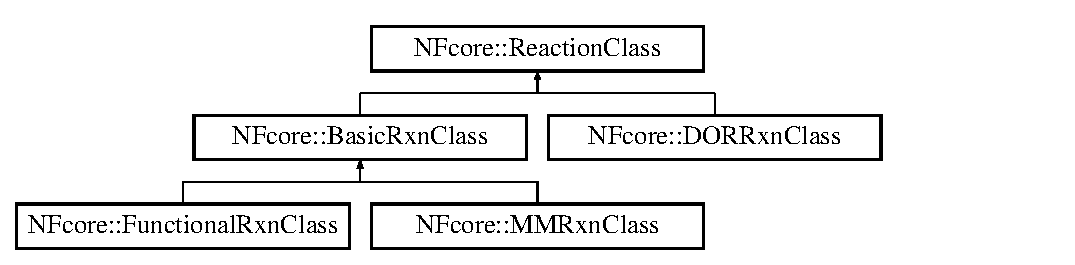
\includegraphics[height=3cm]{classNFcore_1_1ReactionClass}
\end{center}
\end{figure}


\subsection{Detailed Description}
Abstract Base Class that defines the interface for all reaction rules. 

A \doxyref{ReactionClass}{p.}{classNFcore_1_1ReactionClass} represents the set of reactions implied by a single reaction rule along with the rate law and propensity of that reaction rule. ReactionClasses also store information needed to transform reactants. A \doxyref{ReactionClass}{p.}{classNFcore_1_1ReactionClass} keeps a reference to every reactant \doxyref{Molecule}{p.}{classNFcore_1_1Molecule} in the system that might participate in the rule. To determine if a particular set of connected Molecules is a possible reactant, ReactionClasses use TemplateMolecules. ReactionClasses come in several forms based on how reactants are chosen and the rate law. For typical ReactionClasses, each reactant \doxyref{Molecule}{p.}{classNFcore_1_1Molecule} has an equal probability of reacting and therefore reactants are selected to participate at random. However, for ReactionClasses with rates that depend functionally on local context, each reactant will have a different probability and rate of reacting. Such ReactionClasses have a distribution of rates and so we refer to them as Distribution of Rates (DOR) Reactions. DOR Reactions require special handling because the participating reactants must be chosen based on its weighted probability of reacting. There are also reactionClasses that can support functionally defined rate laws and michaelis-menton style reactions. All of these implementing classes are declared in the file reactions.hh. \begin{Desc}
\item[Author:]Michael Sneddon \end{Desc}
\subsection*{Public Member Functions}
\begin{CompactItemize}
\item 
{\bf ReactionClass} (string {\bf name}, double rate, string {\bf baseRateParameterName}, {\bf TransformationSet} $\ast${\bf transformationSet}, {\bf System} $\ast$s)
\item 
virtual {\bf $\sim$ReactionClass} ()
\item 
int {\bf getNumOfReactants} () const 
\item 
string {\bf getName} () const 
\item 
double {\bf getBaseRate} () const 
\item 
int {\bf getRxnType} () const 
\item 
void {\bf setBaseRate} (double newBaseRate, string newBaseRateName)
\item 
void {\bf resetBaseRateFromSystemParamter} ()
\item 
void {\bf setTraversalLimit} (int limit)
\item 
double {\bf get\_\-a} () const 
\item 
virtual void {\bf printDetails} () const 
\item 
void {\bf fire} (double random\_\-A\_\-number)
\item 
virtual void {\bf notifyRateFactorChange} ({\bf Molecule} $\ast$m, int reactantIndex, int rxnListIndex)=0
\item 
virtual int {\bf getDORreactantPosition} () const 
\item 
virtual void {\bf init} ()=0
\item 
virtual void {\bf prepareForSimulation} ()=0
\item 
virtual bool {\bf tryToAdd} ({\bf Molecule} $\ast$m, unsigned int reactantPos)=0
\item 
virtual void {\bf remove} ({\bf Molecule} $\ast$m, unsigned int reactantPos)=0
\item 
virtual double {\bf update\_\-a} ()=0
\item 
void {\bf tag} ()
\item 
virtual unsigned int {\bf getReactantCount} (unsigned int reactantIndex) const =0
\item 
virtual void {\bf printFullDetails} () const =0
\item 
void {\bf setRxnId} (int {\bf rxnId})
\item 
int {\bf getRxnId} () const 
\item 
void {\bf turnOff\_\-OnTheFlyObs} ()
\item 
void {\bf setTotalRateFlag} (bool totalRate)
\item 
void {\bf set\_\-match} (vector$<$ {\bf MappingSet} $\ast$ $>$ \&match\_\-set)
\item 
void {\bf apply} (vector$<$ {\bf Molecule} $\ast$ $>$ \&product\_\-molecules)
\end{CompactItemize}
\subsection*{Static Public Attributes}
\begin{CompactItemize}
\item 
static const int {\bf NO\_\-LIMIT} = -3
\item 
static const int {\bf BASIC\_\-RXN} = 0
\item 
static const int {\bf DOR\_\-RXN} = 1
\item 
static const int {\bf OBS\_\-DEPENDENT\_\-RXN} = 2
\end{CompactItemize}
\subsection*{Protected Member Functions}
\begin{CompactItemize}
\item 
virtual void {\bf pickMappingSets} (double randNumber) const =0
\end{CompactItemize}
\subsection*{Protected Attributes}
\begin{CompactItemize}
\item 
int {\bf rxnId}
\item 
bool {\bf tagged}
\item 
string {\bf name}
\item 
int {\bf reactionType}
\item 
unsigned int {\bf n\_\-reactants}
\item 
{\bf System} $\ast$ {\bf system}
\item 
double {\bf baseRate}
\item 
string {\bf baseRateParameterName}
\item 
double {\bf a}
\item 
unsigned int {\bf fireCounter}
\item 
unsigned int {\bf traversalLimit}
\item 
{\bf TemplateMolecule} $\ast$$\ast$ {\bf reactantTemplates}
\item 
{\bf TransformationSet} $\ast$ {\bf transformationSet}
\item 
{\bf MappingSet} $\ast$$\ast$ {\bf mappingSet}
\item 
bool {\bf onTheFlyObservables}
\item 
bool {\bf isDimerStyle}
\item 
list$<$ {\bf Molecule} $\ast$ $>$ {\bf products}
\item 
list$<$ {\bf Molecule} $\ast$ $>$::iterator {\bf molIter}
\item 
vector$<$ int $>$ {\bf updatedComplexes}
\item 
bool {\bf totalRateFlag}
\end{CompactItemize}
\subsection*{Friends}
\begin{CompactItemize}
\item 
class {\bf MatchSetIter}
\item 
class {\bf Netgen}
\end{CompactItemize}


\subsection{Constructor \& Destructor Documentation}
\index{NFcore::ReactionClass@{NFcore::ReactionClass}!ReactionClass@{ReactionClass}}
\index{ReactionClass@{ReactionClass}!NFcore::ReactionClass@{NFcore::ReactionClass}}
\subsubsection{\setlength{\rightskip}{0pt plus 5cm}ReactionClass::ReactionClass (string {\em name}, double {\em rate}, string {\em baseRateParameterName}, {\bf TransformationSet} $\ast$ {\em transformationSet}, {\bf System} $\ast$ {\em s})}\label{classNFcore_1_1ReactionClass_0ff8307d3ca6e3ff5d738b677a8720d2}


\index{NFcore::ReactionClass@{NFcore::ReactionClass}!$\sim$ReactionClass@{$\sim$ReactionClass}}
\index{$\sim$ReactionClass@{$\sim$ReactionClass}!NFcore::ReactionClass@{NFcore::ReactionClass}}
\subsubsection{\setlength{\rightskip}{0pt plus 5cm}ReactionClass::$\sim$ReactionClass ()\hspace{0.3cm}{\tt  [virtual]}}\label{classNFcore_1_1ReactionClass_a5054d30051d6f349ef15af016791a71}




\subsection{Member Function Documentation}
\index{NFcore::ReactionClass@{NFcore::ReactionClass}!getNumOfReactants@{getNumOfReactants}}
\index{getNumOfReactants@{getNumOfReactants}!NFcore::ReactionClass@{NFcore::ReactionClass}}
\subsubsection{\setlength{\rightskip}{0pt plus 5cm}int NFcore::ReactionClass::getNumOfReactants () const\hspace{0.3cm}{\tt  [inline]}}\label{classNFcore_1_1ReactionClass_907f938981002f15e6c7c6a622ba49a5}


\index{NFcore::ReactionClass@{NFcore::ReactionClass}!getName@{getName}}
\index{getName@{getName}!NFcore::ReactionClass@{NFcore::ReactionClass}}
\subsubsection{\setlength{\rightskip}{0pt plus 5cm}string NFcore::ReactionClass::getName () const\hspace{0.3cm}{\tt  [inline]}}\label{classNFcore_1_1ReactionClass_0aa7c6260c3917d955c49fc00ef0599a}


\index{NFcore::ReactionClass@{NFcore::ReactionClass}!getBaseRate@{getBaseRate}}
\index{getBaseRate@{getBaseRate}!NFcore::ReactionClass@{NFcore::ReactionClass}}
\subsubsection{\setlength{\rightskip}{0pt plus 5cm}double NFcore::ReactionClass::getBaseRate () const\hspace{0.3cm}{\tt  [inline]}}\label{classNFcore_1_1ReactionClass_027dad8c404e44f1f7eb33f94d2736ae}


\index{NFcore::ReactionClass@{NFcore::ReactionClass}!getRxnType@{getRxnType}}
\index{getRxnType@{getRxnType}!NFcore::ReactionClass@{NFcore::ReactionClass}}
\subsubsection{\setlength{\rightskip}{0pt plus 5cm}int NFcore::ReactionClass::getRxnType () const\hspace{0.3cm}{\tt  [inline]}}\label{classNFcore_1_1ReactionClass_0536c0392d78d79af4b3ec29c1588caa}


\index{NFcore::ReactionClass@{NFcore::ReactionClass}!setBaseRate@{setBaseRate}}
\index{setBaseRate@{setBaseRate}!NFcore::ReactionClass@{NFcore::ReactionClass}}
\subsubsection{\setlength{\rightskip}{0pt plus 5cm}void NFcore::ReactionClass::setBaseRate (double {\em newBaseRate}, string {\em newBaseRateName})\hspace{0.3cm}{\tt  [inline]}}\label{classNFcore_1_1ReactionClass_6c9371f5d1fbfbb196c486fce7a68b84}


\index{NFcore::ReactionClass@{NFcore::ReactionClass}!resetBaseRateFromSystemParamter@{resetBaseRateFromSystemParamter}}
\index{resetBaseRateFromSystemParamter@{resetBaseRateFromSystemParamter}!NFcore::ReactionClass@{NFcore::ReactionClass}}
\subsubsection{\setlength{\rightskip}{0pt plus 5cm}void ReactionClass::resetBaseRateFromSystemParamter ()}\label{classNFcore_1_1ReactionClass_bbec0fe13307f807d1c2ca30eb64433d}


\index{NFcore::ReactionClass@{NFcore::ReactionClass}!setTraversalLimit@{setTraversalLimit}}
\index{setTraversalLimit@{setTraversalLimit}!NFcore::ReactionClass@{NFcore::ReactionClass}}
\subsubsection{\setlength{\rightskip}{0pt plus 5cm}void NFcore::ReactionClass::setTraversalLimit (int {\em limit})\hspace{0.3cm}{\tt  [inline]}}\label{classNFcore_1_1ReactionClass_2f4840686ba6027398b1bdc9034742f7}


\index{NFcore::ReactionClass@{NFcore::ReactionClass}!get\_\-a@{get\_\-a}}
\index{get\_\-a@{get\_\-a}!NFcore::ReactionClass@{NFcore::ReactionClass}}
\subsubsection{\setlength{\rightskip}{0pt plus 5cm}double NFcore::ReactionClass::get\_\-a () const\hspace{0.3cm}{\tt  [inline]}}\label{classNFcore_1_1ReactionClass_f605cfc2d20a0e49290a67dfa2e0c918}


\index{NFcore::ReactionClass@{NFcore::ReactionClass}!printDetails@{printDetails}}
\index{printDetails@{printDetails}!NFcore::ReactionClass@{NFcore::ReactionClass}}
\subsubsection{\setlength{\rightskip}{0pt plus 5cm}void ReactionClass::printDetails () const\hspace{0.3cm}{\tt  [virtual]}}\label{classNFcore_1_1ReactionClass_7944db14780627ea05cf290688a8bfd3}




Reimplemented in {\bf NFcore::FunctionalRxnClass} \doxyref{}{p.}{classNFcore_1_1FunctionalRxnClass_54fa8f462e0d990d8b547892fca9b918}, {\bf NFcore::MMRxnClass} \doxyref{}{p.}{classNFcore_1_1MMRxnClass_2dc1bbf290be2f3d535954d006efc385}, and {\bf NFcore::DORRxnClass} \doxyref{}{p.}{classNFcore_1_1DORRxnClass_9d90ba3fc8f0effd97f14080ed76b608}.\index{NFcore::ReactionClass@{NFcore::ReactionClass}!fire@{fire}}
\index{fire@{fire}!NFcore::ReactionClass@{NFcore::ReactionClass}}
\subsubsection{\setlength{\rightskip}{0pt plus 5cm}void ReactionClass::fire (double {\em random\_\-A\_\-number})}\label{classNFcore_1_1ReactionClass_a29cf3993e835405202ca462be86dc0c}


\index{NFcore::ReactionClass@{NFcore::ReactionClass}!notifyRateFactorChange@{notifyRateFactorChange}}
\index{notifyRateFactorChange@{notifyRateFactorChange}!NFcore::ReactionClass@{NFcore::ReactionClass}}
\subsubsection{\setlength{\rightskip}{0pt plus 5cm}virtual void NFcore::ReactionClass::notifyRateFactorChange ({\bf Molecule} $\ast$ {\em m}, int {\em reactantIndex}, int {\em rxnListIndex})\hspace{0.3cm}{\tt  [pure virtual]}}\label{classNFcore_1_1ReactionClass_c18b82dc36c68699c00802201d7745cd}




Implemented in {\bf NFcore::BasicRxnClass} \doxyref{}{p.}{classNFcore_1_1BasicRxnClass_ccc697e4b64efe0d4ced497cc886ece2}, and {\bf NFcore::DORRxnClass} \doxyref{}{p.}{classNFcore_1_1DORRxnClass_ef4d5b83d7f268142af4bbb6c13f89b3}.\index{NFcore::ReactionClass@{NFcore::ReactionClass}!getDORreactantPosition@{getDORreactantPosition}}
\index{getDORreactantPosition@{getDORreactantPosition}!NFcore::ReactionClass@{NFcore::ReactionClass}}
\subsubsection{\setlength{\rightskip}{0pt plus 5cm}virtual int NFcore::ReactionClass::getDORreactantPosition () const\hspace{0.3cm}{\tt  [inline, virtual]}}\label{classNFcore_1_1ReactionClass_06f85ae28c934c344542626c627929e7}




Reimplemented in {\bf NFcore::DORRxnClass} \doxyref{}{p.}{classNFcore_1_1DORRxnClass_2a1fbaba84429f5b076ce40e1848cb65}.\index{NFcore::ReactionClass@{NFcore::ReactionClass}!init@{init}}
\index{init@{init}!NFcore::ReactionClass@{NFcore::ReactionClass}}
\subsubsection{\setlength{\rightskip}{0pt plus 5cm}virtual void NFcore::ReactionClass::init ()\hspace{0.3cm}{\tt  [pure virtual]}}\label{classNFcore_1_1ReactionClass_fa3006801b4fcf821358bfca9bab8aa1}




Implemented in {\bf NFcore::BasicRxnClass} \doxyref{}{p.}{classNFcore_1_1BasicRxnClass_61147eb37d1d45be12a9e77cacd6bb92}, and {\bf NFcore::DORRxnClass} \doxyref{}{p.}{classNFcore_1_1DORRxnClass_bd3127e922a51881509c4958e46fc56f}.\index{NFcore::ReactionClass@{NFcore::ReactionClass}!prepareForSimulation@{prepareForSimulation}}
\index{prepareForSimulation@{prepareForSimulation}!NFcore::ReactionClass@{NFcore::ReactionClass}}
\subsubsection{\setlength{\rightskip}{0pt plus 5cm}virtual void NFcore::ReactionClass::prepareForSimulation ()\hspace{0.3cm}{\tt  [pure virtual]}}\label{classNFcore_1_1ReactionClass_f6466927590b894478fbe765f4da8aad}




Implemented in {\bf NFcore::BasicRxnClass} \doxyref{}{p.}{classNFcore_1_1BasicRxnClass_b96fd7ecb28984d28f0250bb4fc09631}, and {\bf NFcore::DORRxnClass} \doxyref{}{p.}{classNFcore_1_1DORRxnClass_afc1267a5cd558075d87f79837b3dcba}.\index{NFcore::ReactionClass@{NFcore::ReactionClass}!tryToAdd@{tryToAdd}}
\index{tryToAdd@{tryToAdd}!NFcore::ReactionClass@{NFcore::ReactionClass}}
\subsubsection{\setlength{\rightskip}{0pt plus 5cm}virtual bool NFcore::ReactionClass::tryToAdd ({\bf Molecule} $\ast$ {\em m}, unsigned int {\em reactantPos})\hspace{0.3cm}{\tt  [pure virtual]}}\label{classNFcore_1_1ReactionClass_7ef57431ab858d1039e9efedd011f1f0}




Implemented in {\bf NFcore::BasicRxnClass} \doxyref{}{p.}{classNFcore_1_1BasicRxnClass_56e941f00e4f503afb9519a6f23d30fd}, and {\bf NFcore::DORRxnClass} \doxyref{}{p.}{classNFcore_1_1DORRxnClass_d766aeb571ab65fc188ef9fea8212384}.\index{NFcore::ReactionClass@{NFcore::ReactionClass}!remove@{remove}}
\index{remove@{remove}!NFcore::ReactionClass@{NFcore::ReactionClass}}
\subsubsection{\setlength{\rightskip}{0pt plus 5cm}virtual void NFcore::ReactionClass::remove ({\bf Molecule} $\ast$ {\em m}, unsigned int {\em reactantPos})\hspace{0.3cm}{\tt  [pure virtual]}}\label{classNFcore_1_1ReactionClass_e9f356905524d6e370059b1e4ef5754a}




Implemented in {\bf NFcore::BasicRxnClass} \doxyref{}{p.}{classNFcore_1_1BasicRxnClass_4c3f8b5ff51c05a930aeeef6367ced23}, and {\bf NFcore::DORRxnClass} \doxyref{}{p.}{classNFcore_1_1DORRxnClass_724546efe978d79d53744567691bfd99}.\index{NFcore::ReactionClass@{NFcore::ReactionClass}!update\_\-a@{update\_\-a}}
\index{update\_\-a@{update\_\-a}!NFcore::ReactionClass@{NFcore::ReactionClass}}
\subsubsection{\setlength{\rightskip}{0pt plus 5cm}virtual double NFcore::ReactionClass::update\_\-a ()\hspace{0.3cm}{\tt  [pure virtual]}}\label{classNFcore_1_1ReactionClass_f5aed18705e78d14bd1a8f82068add70}




Implemented in {\bf NFcore::BasicRxnClass} \doxyref{}{p.}{classNFcore_1_1BasicRxnClass_9a679d57f4cfdd184f3bf312ecd20cc6}, {\bf NFcore::FunctionalRxnClass} \doxyref{}{p.}{classNFcore_1_1FunctionalRxnClass_23dd5630ec0157ce7ab6d240720a57cb}, {\bf NFcore::MMRxnClass} \doxyref{}{p.}{classNFcore_1_1MMRxnClass_63709cdada0fc7c63125bd2e562f4b42}, and {\bf NFcore::DORRxnClass} \doxyref{}{p.}{classNFcore_1_1DORRxnClass_077d5dc28b205d46a14d22487c08bb7e}.\index{NFcore::ReactionClass@{NFcore::ReactionClass}!tag@{tag}}
\index{tag@{tag}!NFcore::ReactionClass@{NFcore::ReactionClass}}
\subsubsection{\setlength{\rightskip}{0pt plus 5cm}void NFcore::ReactionClass::tag ()\hspace{0.3cm}{\tt  [inline]}}\label{classNFcore_1_1ReactionClass_77c272fe7042f8121a2fefdf3348245c}


\index{NFcore::ReactionClass@{NFcore::ReactionClass}!getReactantCount@{getReactantCount}}
\index{getReactantCount@{getReactantCount}!NFcore::ReactionClass@{NFcore::ReactionClass}}
\subsubsection{\setlength{\rightskip}{0pt plus 5cm}virtual unsigned int NFcore::ReactionClass::getReactantCount (unsigned int {\em reactantIndex}) const\hspace{0.3cm}{\tt  [pure virtual]}}\label{classNFcore_1_1ReactionClass_a39fd321f4d58d79fa72812d65f1c762}




Implemented in {\bf NFcore::BasicRxnClass} \doxyref{}{p.}{classNFcore_1_1BasicRxnClass_908c2d7fdceeb2c77f43d47275b707ff}, and {\bf NFcore::DORRxnClass} \doxyref{}{p.}{classNFcore_1_1DORRxnClass_bff81c460e3398249e095f1f52a60652}.\index{NFcore::ReactionClass@{NFcore::ReactionClass}!printFullDetails@{printFullDetails}}
\index{printFullDetails@{printFullDetails}!NFcore::ReactionClass@{NFcore::ReactionClass}}
\subsubsection{\setlength{\rightskip}{0pt plus 5cm}virtual void NFcore::ReactionClass::printFullDetails () const\hspace{0.3cm}{\tt  [pure virtual]}}\label{classNFcore_1_1ReactionClass_521a0b7a474568522bec973cfa6b5242}




Implemented in {\bf NFcore::BasicRxnClass} \doxyref{}{p.}{classNFcore_1_1BasicRxnClass_552dfb3cbcd194fef08e7c4ba773054e}, and {\bf NFcore::DORRxnClass} \doxyref{}{p.}{classNFcore_1_1DORRxnClass_25114f968aea64b0ba990ce58b974fb5}.\index{NFcore::ReactionClass@{NFcore::ReactionClass}!setRxnId@{setRxnId}}
\index{setRxnId@{setRxnId}!NFcore::ReactionClass@{NFcore::ReactionClass}}
\subsubsection{\setlength{\rightskip}{0pt plus 5cm}void NFcore::ReactionClass::setRxnId (int {\em rxnId})\hspace{0.3cm}{\tt  [inline]}}\label{classNFcore_1_1ReactionClass_0af90982128cc46f1cec0a357abc7ee7}


\index{NFcore::ReactionClass@{NFcore::ReactionClass}!getRxnId@{getRxnId}}
\index{getRxnId@{getRxnId}!NFcore::ReactionClass@{NFcore::ReactionClass}}
\subsubsection{\setlength{\rightskip}{0pt plus 5cm}int NFcore::ReactionClass::getRxnId () const\hspace{0.3cm}{\tt  [inline]}}\label{classNFcore_1_1ReactionClass_cba58796ba1be7b569ba4138820942e0}


\index{NFcore::ReactionClass@{NFcore::ReactionClass}!turnOff\_\-OnTheFlyObs@{turnOff\_\-OnTheFlyObs}}
\index{turnOff\_\-OnTheFlyObs@{turnOff\_\-OnTheFlyObs}!NFcore::ReactionClass@{NFcore::ReactionClass}}
\subsubsection{\setlength{\rightskip}{0pt plus 5cm}void NFcore::ReactionClass::turnOff\_\-OnTheFlyObs ()\hspace{0.3cm}{\tt  [inline]}}\label{classNFcore_1_1ReactionClass_6cacdb25174997f2bc90a8f959dedf99}


\index{NFcore::ReactionClass@{NFcore::ReactionClass}!setTotalRateFlag@{setTotalRateFlag}}
\index{setTotalRateFlag@{setTotalRateFlag}!NFcore::ReactionClass@{NFcore::ReactionClass}}
\subsubsection{\setlength{\rightskip}{0pt plus 5cm}void NFcore::ReactionClass::setTotalRateFlag (bool {\em totalRate})\hspace{0.3cm}{\tt  [inline]}}\label{classNFcore_1_1ReactionClass_06d14b2bec20af725aa125fc7e436e23}


\index{NFcore::ReactionClass@{NFcore::ReactionClass}!set\_\-match@{set\_\-match}}
\index{set\_\-match@{set\_\-match}!NFcore::ReactionClass@{NFcore::ReactionClass}}
\subsubsection{\setlength{\rightskip}{0pt plus 5cm}void NFcore::ReactionClass::set\_\-match (vector$<$ {\bf MappingSet} $\ast$ $>$ \& {\em match\_\-set})}\label{classNFcore_1_1ReactionClass_3f19e59472bec5ae3418697084b07d63}


\index{NFcore::ReactionClass@{NFcore::ReactionClass}!apply@{apply}}
\index{apply@{apply}!NFcore::ReactionClass@{NFcore::ReactionClass}}
\subsubsection{\setlength{\rightskip}{0pt plus 5cm}void NFcore::ReactionClass::apply (vector$<$ {\bf Molecule} $\ast$ $>$ \& {\em product\_\-molecules})}\label{classNFcore_1_1ReactionClass_39b198975902bc86edc320c984a22dcf}


\index{NFcore::ReactionClass@{NFcore::ReactionClass}!pickMappingSets@{pickMappingSets}}
\index{pickMappingSets@{pickMappingSets}!NFcore::ReactionClass@{NFcore::ReactionClass}}
\subsubsection{\setlength{\rightskip}{0pt plus 5cm}virtual void NFcore::ReactionClass::pickMappingSets (double {\em randNumber}) const\hspace{0.3cm}{\tt  [protected, pure virtual]}}\label{classNFcore_1_1ReactionClass_ff3336a876f9e81904ee2b7be86bbdc5}




Implemented in {\bf NFcore::BasicRxnClass} \doxyref{}{p.}{classNFcore_1_1BasicRxnClass_8d194b51f6338bc68bc8440d02249f0e}, and {\bf NFcore::DORRxnClass} \doxyref{}{p.}{classNFcore_1_1DORRxnClass_5d5d078d2a84602132b708a9bcfb078f}.

\subsection{Friends And Related Function Documentation}
\index{NFcore::ReactionClass@{NFcore::ReactionClass}!MatchSetIter@{MatchSetIter}}
\index{MatchSetIter@{MatchSetIter}!NFcore::ReactionClass@{NFcore::ReactionClass}}
\subsubsection{\setlength{\rightskip}{0pt plus 5cm}friend class MatchSetIter\hspace{0.3cm}{\tt  [friend]}}\label{classNFcore_1_1ReactionClass_0c3b7c0fb9a3c68a4bacee6ade128aec}


\index{NFcore::ReactionClass@{NFcore::ReactionClass}!Netgen@{Netgen}}
\index{Netgen@{Netgen}!NFcore::ReactionClass@{NFcore::ReactionClass}}
\subsubsection{\setlength{\rightskip}{0pt plus 5cm}friend class Netgen\hspace{0.3cm}{\tt  [friend]}}\label{classNFcore_1_1ReactionClass_ba6e336204af7fb6e650375559c23f96}




\subsection{Member Data Documentation}
\index{NFcore::ReactionClass@{NFcore::ReactionClass}!NO\_\-LIMIT@{NO\_\-LIMIT}}
\index{NO\_\-LIMIT@{NO\_\-LIMIT}!NFcore::ReactionClass@{NFcore::ReactionClass}}
\subsubsection{\setlength{\rightskip}{0pt plus 5cm}const int {\bf NFcore::ReactionClass::NO\_\-LIMIT} = -3\hspace{0.3cm}{\tt  [static]}}\label{classNFcore_1_1ReactionClass_6f410f39e8be240209cad19f1aab7f48}


\index{NFcore::ReactionClass@{NFcore::ReactionClass}!BASIC\_\-RXN@{BASIC\_\-RXN}}
\index{BASIC\_\-RXN@{BASIC\_\-RXN}!NFcore::ReactionClass@{NFcore::ReactionClass}}
\subsubsection{\setlength{\rightskip}{0pt plus 5cm}const int {\bf NFcore::ReactionClass::BASIC\_\-RXN} = 0\hspace{0.3cm}{\tt  [static]}}\label{classNFcore_1_1ReactionClass_c8ad52c725fef76019bfd0703949fccb}


\index{NFcore::ReactionClass@{NFcore::ReactionClass}!DOR\_\-RXN@{DOR\_\-RXN}}
\index{DOR\_\-RXN@{DOR\_\-RXN}!NFcore::ReactionClass@{NFcore::ReactionClass}}
\subsubsection{\setlength{\rightskip}{0pt plus 5cm}const int {\bf NFcore::ReactionClass::DOR\_\-RXN} = 1\hspace{0.3cm}{\tt  [static]}}\label{classNFcore_1_1ReactionClass_b7bc944fa3a8ebc2d07409324a7ffed3}


\index{NFcore::ReactionClass@{NFcore::ReactionClass}!OBS\_\-DEPENDENT\_\-RXN@{OBS\_\-DEPENDENT\_\-RXN}}
\index{OBS\_\-DEPENDENT\_\-RXN@{OBS\_\-DEPENDENT\_\-RXN}!NFcore::ReactionClass@{NFcore::ReactionClass}}
\subsubsection{\setlength{\rightskip}{0pt plus 5cm}const int {\bf NFcore::ReactionClass::OBS\_\-DEPENDENT\_\-RXN} = 2\hspace{0.3cm}{\tt  [static]}}\label{classNFcore_1_1ReactionClass_fca6966518ab9383d9015010ea8dd0fe}


\index{NFcore::ReactionClass@{NFcore::ReactionClass}!rxnId@{rxnId}}
\index{rxnId@{rxnId}!NFcore::ReactionClass@{NFcore::ReactionClass}}
\subsubsection{\setlength{\rightskip}{0pt plus 5cm}int {\bf NFcore::ReactionClass::rxnId}\hspace{0.3cm}{\tt  [protected]}}\label{classNFcore_1_1ReactionClass_8abf3b468abe85671e742cb4360d1d91}


\index{NFcore::ReactionClass@{NFcore::ReactionClass}!tagged@{tagged}}
\index{tagged@{tagged}!NFcore::ReactionClass@{NFcore::ReactionClass}}
\subsubsection{\setlength{\rightskip}{0pt plus 5cm}bool {\bf NFcore::ReactionClass::tagged}\hspace{0.3cm}{\tt  [protected]}}\label{classNFcore_1_1ReactionClass_faf3e200765ee0d8e757f4970c810ea4}


\index{NFcore::ReactionClass@{NFcore::ReactionClass}!name@{name}}
\index{name@{name}!NFcore::ReactionClass@{NFcore::ReactionClass}}
\subsubsection{\setlength{\rightskip}{0pt plus 5cm}string {\bf NFcore::ReactionClass::name}\hspace{0.3cm}{\tt  [protected]}}\label{classNFcore_1_1ReactionClass_d485c8ab3d93de6f7170afdb895eb251}


\index{NFcore::ReactionClass@{NFcore::ReactionClass}!reactionType@{reactionType}}
\index{reactionType@{reactionType}!NFcore::ReactionClass@{NFcore::ReactionClass}}
\subsubsection{\setlength{\rightskip}{0pt plus 5cm}int {\bf NFcore::ReactionClass::reactionType}\hspace{0.3cm}{\tt  [protected]}}\label{classNFcore_1_1ReactionClass_5c4b85024376502137b82a16af46be32}


\index{NFcore::ReactionClass@{NFcore::ReactionClass}!n\_\-reactants@{n\_\-reactants}}
\index{n\_\-reactants@{n\_\-reactants}!NFcore::ReactionClass@{NFcore::ReactionClass}}
\subsubsection{\setlength{\rightskip}{0pt plus 5cm}unsigned int {\bf NFcore::ReactionClass::n\_\-reactants}\hspace{0.3cm}{\tt  [protected]}}\label{classNFcore_1_1ReactionClass_302fc738473605c9645142943e174f10}


\index{NFcore::ReactionClass@{NFcore::ReactionClass}!system@{system}}
\index{system@{system}!NFcore::ReactionClass@{NFcore::ReactionClass}}
\subsubsection{\setlength{\rightskip}{0pt plus 5cm}{\bf System}$\ast$ {\bf NFcore::ReactionClass::system}\hspace{0.3cm}{\tt  [protected]}}\label{classNFcore_1_1ReactionClass_f1df6e7866c79df25276fa3477d52277}


\index{NFcore::ReactionClass@{NFcore::ReactionClass}!baseRate@{baseRate}}
\index{baseRate@{baseRate}!NFcore::ReactionClass@{NFcore::ReactionClass}}
\subsubsection{\setlength{\rightskip}{0pt plus 5cm}double {\bf NFcore::ReactionClass::baseRate}\hspace{0.3cm}{\tt  [protected]}}\label{classNFcore_1_1ReactionClass_2cf98fbd283cf3a59f05b9a0012904ef}


\index{NFcore::ReactionClass@{NFcore::ReactionClass}!baseRateParameterName@{baseRateParameterName}}
\index{baseRateParameterName@{baseRateParameterName}!NFcore::ReactionClass@{NFcore::ReactionClass}}
\subsubsection{\setlength{\rightskip}{0pt plus 5cm}string {\bf NFcore::ReactionClass::baseRateParameterName}\hspace{0.3cm}{\tt  [protected]}}\label{classNFcore_1_1ReactionClass_684d4c271bb4e4cb5f80074ad135bfb1}


\index{NFcore::ReactionClass@{NFcore::ReactionClass}!a@{a}}
\index{a@{a}!NFcore::ReactionClass@{NFcore::ReactionClass}}
\subsubsection{\setlength{\rightskip}{0pt plus 5cm}double {\bf NFcore::ReactionClass::a}\hspace{0.3cm}{\tt  [protected]}}\label{classNFcore_1_1ReactionClass_da5d8acd819d11a3ec6c95083f0fb569}


\index{NFcore::ReactionClass@{NFcore::ReactionClass}!fireCounter@{fireCounter}}
\index{fireCounter@{fireCounter}!NFcore::ReactionClass@{NFcore::ReactionClass}}
\subsubsection{\setlength{\rightskip}{0pt plus 5cm}unsigned int {\bf NFcore::ReactionClass::fireCounter}\hspace{0.3cm}{\tt  [protected]}}\label{classNFcore_1_1ReactionClass_06902a019dba22c06d1acb00dd6674a9}


\index{NFcore::ReactionClass@{NFcore::ReactionClass}!traversalLimit@{traversalLimit}}
\index{traversalLimit@{traversalLimit}!NFcore::ReactionClass@{NFcore::ReactionClass}}
\subsubsection{\setlength{\rightskip}{0pt plus 5cm}unsigned int {\bf NFcore::ReactionClass::traversalLimit}\hspace{0.3cm}{\tt  [protected]}}\label{classNFcore_1_1ReactionClass_0fc1d55a06daf0108c3fc5ca1de5ec05}


\index{NFcore::ReactionClass@{NFcore::ReactionClass}!reactantTemplates@{reactantTemplates}}
\index{reactantTemplates@{reactantTemplates}!NFcore::ReactionClass@{NFcore::ReactionClass}}
\subsubsection{\setlength{\rightskip}{0pt plus 5cm}{\bf TemplateMolecule}$\ast$$\ast$ {\bf NFcore::ReactionClass::reactantTemplates}\hspace{0.3cm}{\tt  [protected]}}\label{classNFcore_1_1ReactionClass_2ab42a134fc1bc05a4e72e5b897fd89b}


\index{NFcore::ReactionClass@{NFcore::ReactionClass}!transformationSet@{transformationSet}}
\index{transformationSet@{transformationSet}!NFcore::ReactionClass@{NFcore::ReactionClass}}
\subsubsection{\setlength{\rightskip}{0pt plus 5cm}{\bf TransformationSet}$\ast$ {\bf NFcore::ReactionClass::transformationSet}\hspace{0.3cm}{\tt  [protected]}}\label{classNFcore_1_1ReactionClass_7c33db06b734352e9a8f447128135708}


\index{NFcore::ReactionClass@{NFcore::ReactionClass}!mappingSet@{mappingSet}}
\index{mappingSet@{mappingSet}!NFcore::ReactionClass@{NFcore::ReactionClass}}
\subsubsection{\setlength{\rightskip}{0pt plus 5cm}{\bf MappingSet}$\ast$$\ast$ {\bf NFcore::ReactionClass::mappingSet}\hspace{0.3cm}{\tt  [protected]}}\label{classNFcore_1_1ReactionClass_f60ba7f3cec5c45d2a95b4a2c8803983}


\index{NFcore::ReactionClass@{NFcore::ReactionClass}!onTheFlyObservables@{onTheFlyObservables}}
\index{onTheFlyObservables@{onTheFlyObservables}!NFcore::ReactionClass@{NFcore::ReactionClass}}
\subsubsection{\setlength{\rightskip}{0pt plus 5cm}bool {\bf NFcore::ReactionClass::onTheFlyObservables}\hspace{0.3cm}{\tt  [protected]}}\label{classNFcore_1_1ReactionClass_63da6f1b777b52df9e99c83b3df8cea2}


\index{NFcore::ReactionClass@{NFcore::ReactionClass}!isDimerStyle@{isDimerStyle}}
\index{isDimerStyle@{isDimerStyle}!NFcore::ReactionClass@{NFcore::ReactionClass}}
\subsubsection{\setlength{\rightskip}{0pt plus 5cm}bool {\bf NFcore::ReactionClass::isDimerStyle}\hspace{0.3cm}{\tt  [protected]}}\label{classNFcore_1_1ReactionClass_6bb78bb19e15958fa06f01b8ce62f031}


\index{NFcore::ReactionClass@{NFcore::ReactionClass}!products@{products}}
\index{products@{products}!NFcore::ReactionClass@{NFcore::ReactionClass}}
\subsubsection{\setlength{\rightskip}{0pt plus 5cm}list$<${\bf Molecule} $\ast$$>$ {\bf NFcore::ReactionClass::products}\hspace{0.3cm}{\tt  [protected]}}\label{classNFcore_1_1ReactionClass_7f2014a8a0efd0208ace145976b842e9}


\index{NFcore::ReactionClass@{NFcore::ReactionClass}!molIter@{molIter}}
\index{molIter@{molIter}!NFcore::ReactionClass@{NFcore::ReactionClass}}
\subsubsection{\setlength{\rightskip}{0pt plus 5cm}list$<${\bf Molecule} $\ast$$>$::iterator {\bf NFcore::ReactionClass::molIter}\hspace{0.3cm}{\tt  [protected]}}\label{classNFcore_1_1ReactionClass_129bb718109e2b51f4414269fdcaa61c}


\index{NFcore::ReactionClass@{NFcore::ReactionClass}!updatedComplexes@{updatedComplexes}}
\index{updatedComplexes@{updatedComplexes}!NFcore::ReactionClass@{NFcore::ReactionClass}}
\subsubsection{\setlength{\rightskip}{0pt plus 5cm}vector$<$int$>$ {\bf NFcore::ReactionClass::updatedComplexes}\hspace{0.3cm}{\tt  [protected]}}\label{classNFcore_1_1ReactionClass_0324037aa173736a9216a028a86d8ef6}


\index{NFcore::ReactionClass@{NFcore::ReactionClass}!totalRateFlag@{totalRateFlag}}
\index{totalRateFlag@{totalRateFlag}!NFcore::ReactionClass@{NFcore::ReactionClass}}
\subsubsection{\setlength{\rightskip}{0pt plus 5cm}bool {\bf NFcore::ReactionClass::totalRateFlag}\hspace{0.3cm}{\tt  [protected]}}\label{classNFcore_1_1ReactionClass_f6265961b2ed1f058a51b4e055a9c09a}


flag to identify if the macroscopic vs. microscopic rate is to be used (TotalRate = macroscopic) 

The documentation for this class was generated from the following files:\begin{CompactItemize}
\item 
/home/msneddon/eclipse/galileoSR1\_\-cpp/workspace/NFsim/src/NFcore/{\bf NFcore.hh}\item 
/home/msneddon/eclipse/galileoSR1\_\-cpp/workspace/NFsim/src/NFcore/{\bf reactionClass.cpp}\end{CompactItemize}

\section{NFcore::RemoveMoleculeTransform Class Reference}
\label{classNFcore_1_1RemoveMoleculeTransform}\index{NFcore::RemoveMoleculeTransform@{NFcore::RemoveMoleculeTransform}}
{\tt \#include $<$transformation.hh$>$}

Inheritance diagram for NFcore::RemoveMoleculeTransform::\begin{figure}[H]
\begin{center}
\leavevmode
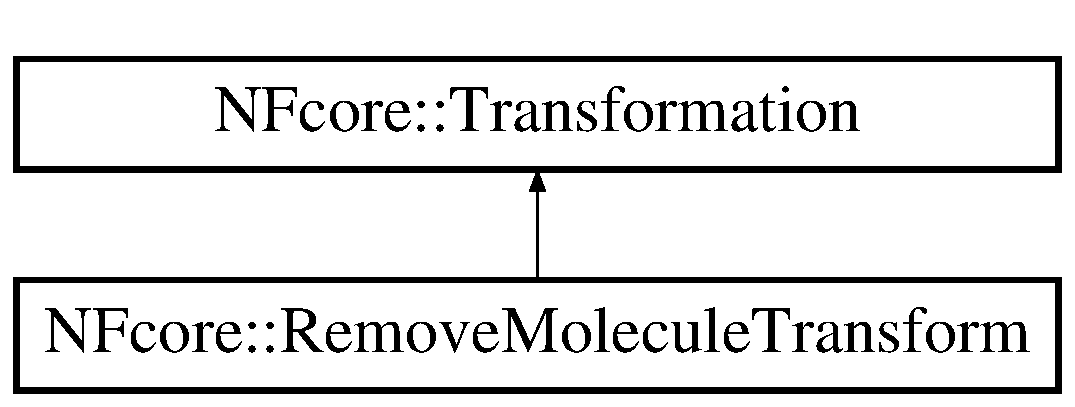
\includegraphics[height=2cm]{classNFcore_1_1RemoveMoleculeTransform}
\end{center}
\end{figure}
\subsection*{Public Member Functions}
\begin{CompactItemize}
\item 
{\bf RemoveMoleculeTransform} ()
\item 
virtual {\bf $\sim$RemoveMoleculeTransform} ()
\item 
virtual void {\bf apply} ({\bf Mapping} $\ast$m, {\bf MappingSet} $\ast$$\ast$ms)
\item 
virtual int {\bf getComponentIndex} () const 
\end{CompactItemize}


\subsection{Constructor \& Destructor Documentation}
\index{NFcore::RemoveMoleculeTransform@{NFcore::RemoveMoleculeTransform}!RemoveMoleculeTransform@{RemoveMoleculeTransform}}
\index{RemoveMoleculeTransform@{RemoveMoleculeTransform}!NFcore::RemoveMoleculeTransform@{NFcore::RemoveMoleculeTransform}}
\subsubsection{\setlength{\rightskip}{0pt plus 5cm}NFcore::RemoveMoleculeTransform::RemoveMoleculeTransform ()\hspace{0.3cm}{\tt  [inline]}}\label{classNFcore_1_1RemoveMoleculeTransform_b42d5054b40ac58524fac25b5f4c407c}


\index{NFcore::RemoveMoleculeTransform@{NFcore::RemoveMoleculeTransform}!$\sim$RemoveMoleculeTransform@{$\sim$RemoveMoleculeTransform}}
\index{$\sim$RemoveMoleculeTransform@{$\sim$RemoveMoleculeTransform}!NFcore::RemoveMoleculeTransform@{NFcore::RemoveMoleculeTransform}}
\subsubsection{\setlength{\rightskip}{0pt plus 5cm}virtual NFcore::RemoveMoleculeTransform::$\sim$RemoveMoleculeTransform ()\hspace{0.3cm}{\tt  [inline, virtual]}}\label{classNFcore_1_1RemoveMoleculeTransform_37e54b1015de2036fe2f3fdd54cef2cb}




\subsection{Member Function Documentation}
\index{NFcore::RemoveMoleculeTransform@{NFcore::RemoveMoleculeTransform}!apply@{apply}}
\index{apply@{apply}!NFcore::RemoveMoleculeTransform@{NFcore::RemoveMoleculeTransform}}
\subsubsection{\setlength{\rightskip}{0pt plus 5cm}void RemoveMoleculeTransform::apply ({\bf Mapping} $\ast$ {\em m}, {\bf MappingSet} $\ast$$\ast$ {\em ms})\hspace{0.3cm}{\tt  [virtual]}}\label{classNFcore_1_1RemoveMoleculeTransform_c277e491df71ad554a93e93ad1e02a7a}




Implements {\bf NFcore::Transformation} \doxyref{}{p.}{classNFcore_1_1Transformation_6a57f607676c92b2465427e57bc7fae5}.\index{NFcore::RemoveMoleculeTransform@{NFcore::RemoveMoleculeTransform}!getComponentIndex@{getComponentIndex}}
\index{getComponentIndex@{getComponentIndex}!NFcore::RemoveMoleculeTransform@{NFcore::RemoveMoleculeTransform}}
\subsubsection{\setlength{\rightskip}{0pt plus 5cm}virtual int NFcore::RemoveMoleculeTransform::getComponentIndex () const\hspace{0.3cm}{\tt  [inline, virtual]}}\label{classNFcore_1_1RemoveMoleculeTransform_02344a04ae5aa77f01786cb88cbe1185}




Implements {\bf NFcore::Transformation} \doxyref{}{p.}{classNFcore_1_1Transformation_2ba394b20768b21ba328431103474607}.

The documentation for this class was generated from the following files:\begin{CompactItemize}
\item 
/home/msneddon/eclipse/ganymede\_\-cpp/workspace/NFsim\_\-svn/src/NFreactions/transformations/{\bf transformation.hh}\item 
/home/msneddon/eclipse/ganymede\_\-cpp/workspace/NFsim\_\-svn/src/NFreactions/transformations/{\bf transformation.cpp}\end{CompactItemize}

\section{NFcore::SpeciesCreator Class Reference}
\label{classNFcore_1_1SpeciesCreator}\index{NFcore::SpeciesCreator@{NFcore::SpeciesCreator}}
{\tt \#include $<$speciesCreator.hh$>$}

\subsection*{Public Member Functions}
\begin{CompactItemize}
\item 
{\bf SpeciesCreator} (vector$<$ {\bf MoleculeType} $\ast$ $>$ \&productMoleculeTypes, vector$<$ vector$<$ int $>$ $>$ \&stateInformation, vector$<$ vector$<$ int $>$ $>$ \&bindingSiteInformation)
\item 
{\bf SpeciesCreator} (vector$<$ {\bf TemplateMolecule} $\ast$ $>$ \&templates)
\item 
{\bf $\sim$SpeciesCreator} ()
\item 
void {\bf create} ()
\end{CompactItemize}
\subsection*{Protected Attributes}
\begin{CompactItemize}
\item 
unsigned int {\bf n\_\-molecules}
\item 
{\bf MoleculeType} $\ast$$\ast$ {\bf moleculeTypes}
\item 
{\bf Molecule} $\ast$$\ast$ {\bf newMoleculeCreations}
\item 
unsigned int {\bf n\_\-ndStates}
\item 
int $\ast$ {\bf ndStateMolecule}
\item 
int $\ast$ {\bf ndStateIndex}
\item 
int $\ast$ {\bf ndStateValue}
\item 
unsigned int {\bf n\_\-bonds}
\item 
int $\ast$ {\bf bMolecule1}
\item 
int $\ast$ {\bf bMolecule2}
\item 
int $\ast$ {\bf bSite1}
\item 
int $\ast$ {\bf bSite2}
\end{CompactItemize}


\subsection{Constructor \& Destructor Documentation}
\index{NFcore::SpeciesCreator@{NFcore::SpeciesCreator}!SpeciesCreator@{SpeciesCreator}}
\index{SpeciesCreator@{SpeciesCreator}!NFcore::SpeciesCreator@{NFcore::SpeciesCreator}}
\subsubsection{\setlength{\rightskip}{0pt plus 5cm}SpeciesCreator::SpeciesCreator (vector$<$ {\bf MoleculeType} $\ast$ $>$ \& {\em productMoleculeTypes}, vector$<$ vector$<$ int $>$ $>$ \& {\em stateInformation}, vector$<$ vector$<$ int $>$ $>$ \& {\em bindingSiteInformation})}\label{classNFcore_1_1SpeciesCreator_32a7b7d2ab8bfba7b95a739bf609c6ca}


\index{NFcore::SpeciesCreator@{NFcore::SpeciesCreator}!SpeciesCreator@{SpeciesCreator}}
\index{SpeciesCreator@{SpeciesCreator}!NFcore::SpeciesCreator@{NFcore::SpeciesCreator}}
\subsubsection{\setlength{\rightskip}{0pt plus 5cm}SpeciesCreator::SpeciesCreator (vector$<$ {\bf TemplateMolecule} $\ast$ $>$ \& {\em templates})}\label{classNFcore_1_1SpeciesCreator_1b35d0e21d38671e8806f0bf48fba56b}


\index{NFcore::SpeciesCreator@{NFcore::SpeciesCreator}!$\sim$SpeciesCreator@{$\sim$SpeciesCreator}}
\index{$\sim$SpeciesCreator@{$\sim$SpeciesCreator}!NFcore::SpeciesCreator@{NFcore::SpeciesCreator}}
\subsubsection{\setlength{\rightskip}{0pt plus 5cm}SpeciesCreator::$\sim$SpeciesCreator ()}\label{classNFcore_1_1SpeciesCreator_747ee43ff8c096c2db21bd5c66d94260}




\subsection{Member Function Documentation}
\index{NFcore::SpeciesCreator@{NFcore::SpeciesCreator}!create@{create}}
\index{create@{create}!NFcore::SpeciesCreator@{NFcore::SpeciesCreator}}
\subsubsection{\setlength{\rightskip}{0pt plus 5cm}void SpeciesCreator::create ()}\label{classNFcore_1_1SpeciesCreator_10a943ceb038c781102a5a31777b48c0}




\subsection{Member Data Documentation}
\index{NFcore::SpeciesCreator@{NFcore::SpeciesCreator}!n\_\-molecules@{n\_\-molecules}}
\index{n\_\-molecules@{n\_\-molecules}!NFcore::SpeciesCreator@{NFcore::SpeciesCreator}}
\subsubsection{\setlength{\rightskip}{0pt plus 5cm}unsigned int {\bf NFcore::SpeciesCreator::n\_\-molecules}\hspace{0.3cm}{\tt  [protected]}}\label{classNFcore_1_1SpeciesCreator_b7cd601dd7e66e075593c073ece2c200}


\index{NFcore::SpeciesCreator@{NFcore::SpeciesCreator}!moleculeTypes@{moleculeTypes}}
\index{moleculeTypes@{moleculeTypes}!NFcore::SpeciesCreator@{NFcore::SpeciesCreator}}
\subsubsection{\setlength{\rightskip}{0pt plus 5cm}{\bf MoleculeType}$\ast$$\ast$ {\bf NFcore::SpeciesCreator::moleculeTypes}\hspace{0.3cm}{\tt  [protected]}}\label{classNFcore_1_1SpeciesCreator_1a90c794aa72f83acea1d00715e66759}


\index{NFcore::SpeciesCreator@{NFcore::SpeciesCreator}!newMoleculeCreations@{newMoleculeCreations}}
\index{newMoleculeCreations@{newMoleculeCreations}!NFcore::SpeciesCreator@{NFcore::SpeciesCreator}}
\subsubsection{\setlength{\rightskip}{0pt plus 5cm}{\bf Molecule}$\ast$$\ast$ {\bf NFcore::SpeciesCreator::newMoleculeCreations}\hspace{0.3cm}{\tt  [protected]}}\label{classNFcore_1_1SpeciesCreator_af8a0cc618176574ce9a6689fa9e0161}


\index{NFcore::SpeciesCreator@{NFcore::SpeciesCreator}!n\_\-ndStates@{n\_\-ndStates}}
\index{n\_\-ndStates@{n\_\-ndStates}!NFcore::SpeciesCreator@{NFcore::SpeciesCreator}}
\subsubsection{\setlength{\rightskip}{0pt plus 5cm}unsigned int {\bf NFcore::SpeciesCreator::n\_\-ndStates}\hspace{0.3cm}{\tt  [protected]}}\label{classNFcore_1_1SpeciesCreator_365e16eac7ee9e4daa304b122ddb28c8}


\index{NFcore::SpeciesCreator@{NFcore::SpeciesCreator}!ndStateMolecule@{ndStateMolecule}}
\index{ndStateMolecule@{ndStateMolecule}!NFcore::SpeciesCreator@{NFcore::SpeciesCreator}}
\subsubsection{\setlength{\rightskip}{0pt plus 5cm}int$\ast$ {\bf NFcore::SpeciesCreator::ndStateMolecule}\hspace{0.3cm}{\tt  [protected]}}\label{classNFcore_1_1SpeciesCreator_3ec95970f113d58eb2f13771c42d21c1}


\index{NFcore::SpeciesCreator@{NFcore::SpeciesCreator}!ndStateIndex@{ndStateIndex}}
\index{ndStateIndex@{ndStateIndex}!NFcore::SpeciesCreator@{NFcore::SpeciesCreator}}
\subsubsection{\setlength{\rightskip}{0pt plus 5cm}int$\ast$ {\bf NFcore::SpeciesCreator::ndStateIndex}\hspace{0.3cm}{\tt  [protected]}}\label{classNFcore_1_1SpeciesCreator_89b760b9e4217eb260dd7ac56561cb45}


\index{NFcore::SpeciesCreator@{NFcore::SpeciesCreator}!ndStateValue@{ndStateValue}}
\index{ndStateValue@{ndStateValue}!NFcore::SpeciesCreator@{NFcore::SpeciesCreator}}
\subsubsection{\setlength{\rightskip}{0pt plus 5cm}int$\ast$ {\bf NFcore::SpeciesCreator::ndStateValue}\hspace{0.3cm}{\tt  [protected]}}\label{classNFcore_1_1SpeciesCreator_e66608c21948190c5922257f106569a6}


\index{NFcore::SpeciesCreator@{NFcore::SpeciesCreator}!n\_\-bonds@{n\_\-bonds}}
\index{n\_\-bonds@{n\_\-bonds}!NFcore::SpeciesCreator@{NFcore::SpeciesCreator}}
\subsubsection{\setlength{\rightskip}{0pt plus 5cm}unsigned int {\bf NFcore::SpeciesCreator::n\_\-bonds}\hspace{0.3cm}{\tt  [protected]}}\label{classNFcore_1_1SpeciesCreator_ae6b5119f145f5f9dd90d3fec3ecc5ef}


\index{NFcore::SpeciesCreator@{NFcore::SpeciesCreator}!bMolecule1@{bMolecule1}}
\index{bMolecule1@{bMolecule1}!NFcore::SpeciesCreator@{NFcore::SpeciesCreator}}
\subsubsection{\setlength{\rightskip}{0pt plus 5cm}int$\ast$ {\bf NFcore::SpeciesCreator::bMolecule1}\hspace{0.3cm}{\tt  [protected]}}\label{classNFcore_1_1SpeciesCreator_7a98b3473dbe2d38f2cc8ff88c47207b}


\index{NFcore::SpeciesCreator@{NFcore::SpeciesCreator}!bMolecule2@{bMolecule2}}
\index{bMolecule2@{bMolecule2}!NFcore::SpeciesCreator@{NFcore::SpeciesCreator}}
\subsubsection{\setlength{\rightskip}{0pt plus 5cm}int$\ast$ {\bf NFcore::SpeciesCreator::bMolecule2}\hspace{0.3cm}{\tt  [protected]}}\label{classNFcore_1_1SpeciesCreator_8d4caa643ae21910fc49577331b6e9aa}


\index{NFcore::SpeciesCreator@{NFcore::SpeciesCreator}!bSite1@{bSite1}}
\index{bSite1@{bSite1}!NFcore::SpeciesCreator@{NFcore::SpeciesCreator}}
\subsubsection{\setlength{\rightskip}{0pt plus 5cm}int$\ast$ {\bf NFcore::SpeciesCreator::bSite1}\hspace{0.3cm}{\tt  [protected]}}\label{classNFcore_1_1SpeciesCreator_5c07bfe05a98d21564079015559defc0}


\index{NFcore::SpeciesCreator@{NFcore::SpeciesCreator}!bSite2@{bSite2}}
\index{bSite2@{bSite2}!NFcore::SpeciesCreator@{NFcore::SpeciesCreator}}
\subsubsection{\setlength{\rightskip}{0pt plus 5cm}int$\ast$ {\bf NFcore::SpeciesCreator::bSite2}\hspace{0.3cm}{\tt  [protected]}}\label{classNFcore_1_1SpeciesCreator_709c3005ce881579df83cb7c3e0c45aa}




The documentation for this class was generated from the following files:\begin{CompactItemize}
\item 
/home/msneddon/eclipse/indigo/workspace/NFsim/src/NFreactions/transformations/{\bf speciesCreator.hh}\item 
/home/msneddon/eclipse/indigo/workspace/NFsim/src/NFreactions/transformations/{\bf speciesCreator.cpp}\end{CompactItemize}

\section{NFcore::StateChangeTransform Class Reference}
\label{classNFcore_1_1StateChangeTransform}\index{NFcore::StateChangeTransform@{NFcore::StateChangeTransform}}
{\tt \#include $<$transformation.hh$>$}

Inheritance diagram for NFcore::StateChangeTransform::\begin{figure}[H]
\begin{center}
\leavevmode
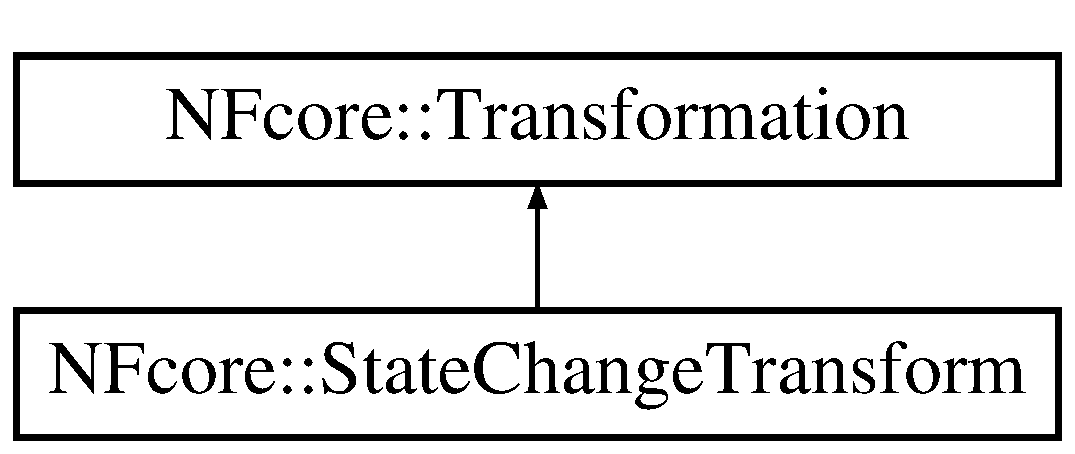
\includegraphics[height=2cm]{classNFcore_1_1StateChangeTransform}
\end{center}
\end{figure}
\subsection*{Public Member Functions}
\begin{CompactItemize}
\item 
{\bf StateChangeTransform} (int {\bf cIndex}, int {\bf newValue})
\item 
virtual {\bf $\sim$StateChangeTransform} ()
\item 
virtual void {\bf apply} ({\bf Mapping} $\ast$m, {\bf MappingSet} $\ast$$\ast$ms)
\item 
virtual int {\bf getComponentIndex} () const 
\end{CompactItemize}
\subsection*{Protected Attributes}
\begin{CompactItemize}
\item 
int {\bf cIndex}
\item 
int {\bf newValue}
\end{CompactItemize}


\subsection{Constructor \& Destructor Documentation}
\index{NFcore::StateChangeTransform@{NFcore::StateChangeTransform}!StateChangeTransform@{StateChangeTransform}}
\index{StateChangeTransform@{StateChangeTransform}!NFcore::StateChangeTransform@{NFcore::StateChangeTransform}}
\subsubsection{\setlength{\rightskip}{0pt plus 5cm}StateChangeTransform::StateChangeTransform (int {\em cIndex}, int {\em newValue})}\label{classNFcore_1_1StateChangeTransform_9d4a2049b1dc64a9db7eeb65048794b4}


\index{NFcore::StateChangeTransform@{NFcore::StateChangeTransform}!$\sim$StateChangeTransform@{$\sim$StateChangeTransform}}
\index{$\sim$StateChangeTransform@{$\sim$StateChangeTransform}!NFcore::StateChangeTransform@{NFcore::StateChangeTransform}}
\subsubsection{\setlength{\rightskip}{0pt plus 5cm}virtual NFcore::StateChangeTransform::$\sim$StateChangeTransform ()\hspace{0.3cm}{\tt  [inline, virtual]}}\label{classNFcore_1_1StateChangeTransform_43f76f8201ae436c4bf50b27739c2e63}




\subsection{Member Function Documentation}
\index{NFcore::StateChangeTransform@{NFcore::StateChangeTransform}!apply@{apply}}
\index{apply@{apply}!NFcore::StateChangeTransform@{NFcore::StateChangeTransform}}
\subsubsection{\setlength{\rightskip}{0pt plus 5cm}void StateChangeTransform::apply ({\bf Mapping} $\ast$ {\em m}, {\bf MappingSet} $\ast$$\ast$ {\em ms})\hspace{0.3cm}{\tt  [virtual]}}\label{classNFcore_1_1StateChangeTransform_a74df84e5d6eac3709ea4636a674edee}




Implements {\bf NFcore::Transformation} \doxyref{}{p.}{classNFcore_1_1Transformation_6a57f607676c92b2465427e57bc7fae5}.\index{NFcore::StateChangeTransform@{NFcore::StateChangeTransform}!getComponentIndex@{getComponentIndex}}
\index{getComponentIndex@{getComponentIndex}!NFcore::StateChangeTransform@{NFcore::StateChangeTransform}}
\subsubsection{\setlength{\rightskip}{0pt plus 5cm}virtual int NFcore::StateChangeTransform::getComponentIndex () const\hspace{0.3cm}{\tt  [inline, virtual]}}\label{classNFcore_1_1StateChangeTransform_5ae788f00d608b4d4417408d2559a0fb}




Implements {\bf NFcore::Transformation} \doxyref{}{p.}{classNFcore_1_1Transformation_2ba394b20768b21ba328431103474607}.

\subsection{Member Data Documentation}
\index{NFcore::StateChangeTransform@{NFcore::StateChangeTransform}!cIndex@{cIndex}}
\index{cIndex@{cIndex}!NFcore::StateChangeTransform@{NFcore::StateChangeTransform}}
\subsubsection{\setlength{\rightskip}{0pt plus 5cm}int {\bf NFcore::StateChangeTransform::cIndex}\hspace{0.3cm}{\tt  [protected]}}\label{classNFcore_1_1StateChangeTransform_8b1f5886dd11dafcfd947c30a1a421de}


\index{NFcore::StateChangeTransform@{NFcore::StateChangeTransform}!newValue@{newValue}}
\index{newValue@{newValue}!NFcore::StateChangeTransform@{NFcore::StateChangeTransform}}
\subsubsection{\setlength{\rightskip}{0pt plus 5cm}int {\bf NFcore::StateChangeTransform::newValue}\hspace{0.3cm}{\tt  [protected]}}\label{classNFcore_1_1StateChangeTransform_e0572474fd78825928ef9b9a3d926681}




The documentation for this class was generated from the following files:\begin{CompactItemize}
\item 
/home/msneddon/eclipse/ganymede\_\-cpp/workspace/NFsim\_\-svn/src/NFreactions/transformations/{\bf transformation.hh}\item 
/home/msneddon/eclipse/ganymede\_\-cpp/workspace/NFsim\_\-svn/src/NFreactions/transformations/{\bf transformation.cpp}\end{CompactItemize}

\section{NFcore::StateCounter Class Reference}
\label{classNFcore_1_1StateCounter}\index{NFcore::StateCounter@{NFcore::StateCounter}}
{\tt \#include $<$NFfunction.hh$>$}

\subsection*{Public Member Functions}
\begin{CompactItemize}
\item 
{\bf StateCounter} (string {\bf name}, {\bf MoleculeType} $\ast${\bf mt}, string stateName)
\item 
{\bf $\sim$StateCounter} ()
\item 
void {\bf add} ({\bf Molecule} $\ast$m)
\item 
void {\bf reset} ()
\item 
int {\bf getValue} () const 
\end{CompactItemize}
\subsection*{Public Attributes}
\begin{CompactItemize}
\item 
string {\bf name}
\item 
{\bf MoleculeType} $\ast$ {\bf mt}
\item 
int {\bf stateIndex}
\item 
double {\bf value}
\end{CompactItemize}


\subsection{Constructor \& Destructor Documentation}
\index{NFcore::StateCounter@{NFcore::StateCounter}!StateCounter@{StateCounter}}
\index{StateCounter@{StateCounter}!NFcore::StateCounter@{NFcore::StateCounter}}
\subsubsection{\setlength{\rightskip}{0pt plus 5cm}StateCounter::StateCounter (string {\em name}, {\bf MoleculeType} $\ast$ {\em mt}, string {\em stateName})}\label{classNFcore_1_1StateCounter_29a85dac199f2bc9ba0939f167c93ffd}


\index{NFcore::StateCounter@{NFcore::StateCounter}!$\sim$StateCounter@{$\sim$StateCounter}}
\index{$\sim$StateCounter@{$\sim$StateCounter}!NFcore::StateCounter@{NFcore::StateCounter}}
\subsubsection{\setlength{\rightskip}{0pt plus 5cm}StateCounter::$\sim$StateCounter ()}\label{classNFcore_1_1StateCounter_60532266957dbb17a58dd6cd2551a861}




\subsection{Member Function Documentation}
\index{NFcore::StateCounter@{NFcore::StateCounter}!add@{add}}
\index{add@{add}!NFcore::StateCounter@{NFcore::StateCounter}}
\subsubsection{\setlength{\rightskip}{0pt plus 5cm}void StateCounter::add ({\bf Molecule} $\ast$ {\em m})}\label{classNFcore_1_1StateCounter_76d0f49396f1931882fa05cfee1f91f6}


\index{NFcore::StateCounter@{NFcore::StateCounter}!reset@{reset}}
\index{reset@{reset}!NFcore::StateCounter@{NFcore::StateCounter}}
\subsubsection{\setlength{\rightskip}{0pt plus 5cm}void NFcore::StateCounter::reset ()\hspace{0.3cm}{\tt  [inline]}}\label{classNFcore_1_1StateCounter_b389c343c4286183d501e3d1ade3e2d4}


\index{NFcore::StateCounter@{NFcore::StateCounter}!getValue@{getValue}}
\index{getValue@{getValue}!NFcore::StateCounter@{NFcore::StateCounter}}
\subsubsection{\setlength{\rightskip}{0pt plus 5cm}int NFcore::StateCounter::getValue () const\hspace{0.3cm}{\tt  [inline]}}\label{classNFcore_1_1StateCounter_738f27e703b561b552748dff71fa85b6}




\subsection{Member Data Documentation}
\index{NFcore::StateCounter@{NFcore::StateCounter}!name@{name}}
\index{name@{name}!NFcore::StateCounter@{NFcore::StateCounter}}
\subsubsection{\setlength{\rightskip}{0pt plus 5cm}string {\bf NFcore::StateCounter::name}}\label{classNFcore_1_1StateCounter_f33e6c1ac6e69d74b24f6b9ca3238193}


\index{NFcore::StateCounter@{NFcore::StateCounter}!mt@{mt}}
\index{mt@{mt}!NFcore::StateCounter@{NFcore::StateCounter}}
\subsubsection{\setlength{\rightskip}{0pt plus 5cm}{\bf MoleculeType}$\ast$ {\bf NFcore::StateCounter::mt}}\label{classNFcore_1_1StateCounter_415dd923cb75e9da42f3f5ca44bcee49}


\index{NFcore::StateCounter@{NFcore::StateCounter}!stateIndex@{stateIndex}}
\index{stateIndex@{stateIndex}!NFcore::StateCounter@{NFcore::StateCounter}}
\subsubsection{\setlength{\rightskip}{0pt plus 5cm}int {\bf NFcore::StateCounter::stateIndex}}\label{classNFcore_1_1StateCounter_0b039d4ee92aae9dd6b841f8cea13cd3}


\index{NFcore::StateCounter@{NFcore::StateCounter}!value@{value}}
\index{value@{value}!NFcore::StateCounter@{NFcore::StateCounter}}
\subsubsection{\setlength{\rightskip}{0pt plus 5cm}double {\bf NFcore::StateCounter::value}}\label{classNFcore_1_1StateCounter_c170ba269add82d4722bc386b3532bdb}




The documentation for this class was generated from the following files:\begin{CompactItemize}
\item 
/home/msneddon/eclipse/ganymede\_\-cpp/workspace/NFsim\_\-svn/src/NFfunction/{\bf NFfunction.hh}\item 
/home/msneddon/eclipse/ganymede\_\-cpp/workspace/NFsim\_\-svn/src/NFfunction/{\bf function.cpp}\end{CompactItemize}

\section{NFcore::System Class Reference}
\label{classNFcore_1_1System}\index{NFcore::System@{NFcore::System}}
{\tt \#include $<$NFcore.hh$>$}



\subsection{Detailed Description}
The main class that begins and runs simulations. 

This class is what runs the actual simulation. It keeps lists of all MoleculeTypes that exist and all Reactions that can operate on those moleculeTypes. It also contains the function (named sim) which runs the main simulation loop. To create a new \doxyref{System}{p.}{classNFcore_1_1System}, first add all MoleculeTypes, all reactions, then call the function \doxyref{prepareForSimulation()}{p.}{classNFcore_1_1System_6caa03d1c59dc7044d81d4666b306fe7}. Then call the sim function as many times as you like. Output is printed to the given output file and lists all observables per time according to how often you want values recorded. \begin{Desc}
\item[Author:]Michael Sneddon \end{Desc}
\subsection*{Public Member Functions}
\begin{CompactItemize}
\item 
{\bf System} (string {\bf name})
\item 
{\bf System} (string {\bf name}, bool {\bf useComplex})
\item 
{\bf System} (string {\bf name}, bool {\bf useComplex}, int {\bf globalMoleculeLimit})
\item 
{\bf $\sim$System} ()
\item 
string {\bf getName} () const 
\item 
bool {\bf isUsingComplex} ()
\item 
bool {\bf isOutputtingBinary} ()
\item 
double {\bf getCurrentTime} () const 
\item 
int {\bf getGlobalMoleculeLimit} () const 
\item 
int {\bf getMolObsCount} (int moleculeTypeIndex, int observableIndex) const 
\item 
{\bf Observable} $\ast$ {\bf getObservableByName} (string obsName)
\item 
double {\bf getAverageGroupValue} (string groupName, int valIndex)
\item 
{\bf ReactionClass} $\ast$ {\bf getReaction} (int rIndex)
\item 
{\bf MoleculeType} $\ast$ {\bf getMoleculeType} (int mtIndex)
\item 
{\bf MoleculeType} $\ast$ {\bf getMoleculeTypeByName} (string {\bf name})
\item 
int {\bf getNumOfMoleculeTypes} ()
\item 
{\bf Molecule} $\ast$ {\bf getMoleculeByUid} (int uid)
\item 
int {\bf getNumOfMolecules} ()
\item 
int {\bf addMoleculeType} ({\bf MoleculeType} $\ast$moleculeType)
\item 
void {\bf addReaction} ({\bf ReactionClass} $\ast$reaction)
\item 
void {\bf addNecessaryUpdateReaction} ({\bf ReactionClass} $\ast$reaction)
\item 
bool {\bf addGlobalFunction} ({\bf GlobalFunction} $\ast$gf)
\item 
{\bf GlobalFunction} $\ast$ {\bf getGlobalFunctionByName} (string fName)
\item 
bool {\bf addCompositeFunction} ({\bf CompositeFunction} $\ast$cf)
\item 
{\bf CompositeFunction} $\ast$ {\bf getCompositeFunctionByName} (string fName)
\item 
void {\bf finalizeCompositeFunctions} ()
\item 
void {\bf printAllFunctions} ()
\item 
bool {\bf saveSpecies} ()
\item 
bool {\bf saveSpecies} (string filename)
\item 
{\bf LocalFunction} $\ast$ {\bf getLocalFunctionByName} (string fName)
\item 
void {\bf prepareForSimulation} ()
\item 
void {\bf setUniversalTraversalLimit} (int utl)
\item 
void {\bf setOutputToBinary} ()
\item 
void {\bf registerOutputFileLocation} (string filename)
\item 
void {\bf setDumpOutputter} ({\bf DumpSystem} $\ast${\bf ds})
\item 
void {\bf tryToDump} ()
\item 
void {\bf turnOnGlobalFuncOut} ()
\item 
void {\bf turnOffGlobalFuncOut} ()
\item 
void {\bf tagReaction} (int rID)
\item 
void {\bf addLocalFunction} ({\bf LocalFunction} $\ast$lf)
\item 
void {\bf getLocalFunction} (string funcName) const 
\item 
void {\bf outputAllObservableNames} ()
\item 
void {\bf outputAllObservableCounts} ()
\item 
void {\bf outputAllObservableCounts} (double cSampleTime)
\item 
void {\bf outputAllObservableCounts} (double cSampleTime, int eventCounter)
\item 
int {\bf getNumOfSpeciesObs} () const 
\item 
{\bf Observable} $\ast$ {\bf getSpeciesObs} (int index) const 
\item 
void {\bf printAllReactions} ()
\item 
void {\bf printIndexAndNames} ()
\item 
void {\bf printAllMoleculeTypes} ()
\item 
void {\bf printAllObservableCounts} ()
\item 
void {\bf printAllObservableCounts} (double cSampleTime)
\item 
void {\bf printAllObservableCounts} (double cSampleTime, int eventCounter)
\item 
void {\bf update\_\-A\_\-tot} ({\bf ReactionClass} $\ast$r, double old\_\-a, double new\_\-a)
\item 
void {\bf evaluateAllLocalFunctions} ()
\item 
void {\bf addObservableForOutput} ({\bf Observable} $\ast$o)
\item 
void {\bf addOutputter} ({\bf Outputter} $\ast$op)
\item 
void {\bf dumpOutputters} ()
\item 
double {\bf sim} (double time, long int sampleTimes)
\item 
double {\bf sim} (double time, long int sampleTimes, bool verbose)
\item 
double {\bf stepTo} (double stoppingTime)
\item 
void {\bf singleStep} ()
\item 
void {\bf equilibrate} (double duration)
\item 
void {\bf equilibrate} (double duration, int statusReports)
\item 
void {\bf registerRxnIndex} (int rxnId, int rxnPos, int rxnIndex)
\item 
int {\bf getRxnIndex} (int rxnId, int rxnPos) const 
\item 
void {\bf turnOff\_\-OnTheFlyObs} ()
\item 
void {\bf turnOnOutputEventCounter} ()
\item 
void {\bf addParameter} (string {\bf name}, double value)
\item 
double {\bf getParameter} (string {\bf name})
\item 
void {\bf setParameter} (string {\bf name}, double value)
\item 
void {\bf updateSystemWithNewParameters} ()
\item 
void {\bf printAllParameters} ()
\item 
{\bf NFstream} \& {\bf getOutputFileStream} ()
\item 
{\bf ComplexList} \& {\bf getAllComplexes} ()
\item 
void {\bf turnOnCSVformat} ()
\end{CompactItemize}
\subsection*{Static Public Attributes}
\begin{CompactItemize}
\item 
static int {\bf NULL\_\-EVENT\_\-COUNTER} = 0
\end{CompactItemize}
\subsection*{Protected Member Functions}
\begin{CompactItemize}
\item 
double {\bf get\_\-A\_\-tot} () const 
\item 
double {\bf recompute\_\-A\_\-tot} ()
\item 
double {\bf getNextRxn} ()
\item 
void {\bf outputGroupDataHeader} ()
\item 
void {\bf outputAllPropensities} (double time, int rxnFired)
\end{CompactItemize}
\subsection*{Protected Attributes}
\begin{CompactItemize}
\item 
string {\bf name}
\item 
bool {\bf useComplex}
\item 
bool {\bf useBinaryOutput}
\item 
int {\bf universalTraversalLimit}
\item 
bool {\bf onTheFlyObservables}
\item 
bool {\bf outputGlobalFunctionValues}
\item 
int {\bf globalMoleculeLimit}
\item 
bool {\bf outputEventCounter}
\item 
int {\bf globalEventCounter}
\item 
vector$<$ {\bf MoleculeType} $\ast$ $>$ {\bf allMoleculeTypes}
\item 
vector$<$ {\bf ReactionClass} $\ast$ $>$ {\bf allReactions}
\item 
vector$<$ {\bf Outputter} $\ast$ $>$ {\bf allOutputters}
\item 
{\bf ComplexList} {\bf allComplexes}
\item 
vector$<$ {\bf Observable} $\ast$ $>$ {\bf obsToOutput}
\item 
vector$<$ {\bf Observable} $\ast$ $>$ {\bf speciesObservables}
\item 
{\bf DumpSystem} $\ast$ {\bf ds}
\item 
vector$<$ {\bf GlobalFunction} $\ast$ $>$ {\bf globalFunctions}
\item 
vector$<$ {\bf LocalFunction} $\ast$ $>$ {\bf localFunctions}
\item 
vector$<$ {\bf ReactionClass} $\ast$ $>$ {\bf necessaryUpdateRxns}
\item 
vector$<$ {\bf CompositeFunction} $\ast$ $>$ {\bf compositeFunctions}
\item 
double {\bf a\_\-tot}
\item 
double {\bf current\_\-time}
\item 
{\bf ReactionClass} $\ast$ {\bf nextReaction}
\item 
{\bf NFstream} {\bf outputFileStream}
\item 
ofstream {\bf propensityDumpStream}
\item 
bool {\bf csvFormat}
\item 
int $\ast$$\ast$ {\bf rxnIndexMap}
\item 
map$<$ string, double $>$ {\bf paramMap}
\item 
{\bf ReactionSelector} $\ast$ {\bf selector}
\end{CompactItemize}
\subsection*{Friends}
\begin{CompactItemize}
\item 
class {\bf Netgen}
\end{CompactItemize}


\subsection{Constructor \& Destructor Documentation}
\index{NFcore::System@{NFcore::System}!System@{System}}
\index{System@{System}!NFcore::System@{NFcore::System}}
\subsubsection{\setlength{\rightskip}{0pt plus 5cm}System::System (string {\em name})}\label{classNFcore_1_1System_bba58818fedf3ef9af5e28e5023e2daa}


creates a system with the given name that does not keep track dynamically of complex formation \index{NFcore::System@{NFcore::System}!System@{System}}
\index{System@{System}!NFcore::System@{NFcore::System}}
\subsubsection{\setlength{\rightskip}{0pt plus 5cm}System::System (string {\em name}, bool {\em useComplex})}\label{classNFcore_1_1System_7ea6dc6d40f2c519f1a3eb55c5e4775c}


creates a system that keeps track of complex formation if the setComplex parameter is set to true \index{NFcore::System@{NFcore::System}!System@{System}}
\index{System@{System}!NFcore::System@{NFcore::System}}
\subsubsection{\setlength{\rightskip}{0pt plus 5cm}System::System (string {\em name}, bool {\em useComplex}, int {\em globalMoleculeLimit})}\label{classNFcore_1_1System_09f875df922ae99a09c2bebdb74ba593}


creates a system that keeps track of complex formation if the setComplex parameter is set to true \index{NFcore::System@{NFcore::System}!$\sim$System@{$\sim$System}}
\index{$\sim$System@{$\sim$System}!NFcore::System@{NFcore::System}}
\subsubsection{\setlength{\rightskip}{0pt plus 5cm}System::$\sim$System ()}\label{classNFcore_1_1System_3be70bb338e3f062f821173fd15680d0}


destroys the system and cleans up all memory associated with it 

\subsection{Member Function Documentation}
\index{NFcore::System@{NFcore::System}!getName@{getName}}
\index{getName@{getName}!NFcore::System@{NFcore::System}}
\subsubsection{\setlength{\rightskip}{0pt plus 5cm}string NFcore::System::getName () const\hspace{0.3cm}{\tt  [inline]}}\label{classNFcore_1_1System_11395716c7875a899b5b05549e95ffa7}


\index{NFcore::System@{NFcore::System}!isUsingComplex@{isUsingComplex}}
\index{isUsingComplex@{isUsingComplex}!NFcore::System@{NFcore::System}}
\subsubsection{\setlength{\rightskip}{0pt plus 5cm}bool NFcore::System::isUsingComplex ()\hspace{0.3cm}{\tt  [inline]}}\label{classNFcore_1_1System_8c9531facb736ba2a737ff47c6a9347c}


\index{NFcore::System@{NFcore::System}!isOutputtingBinary@{isOutputtingBinary}}
\index{isOutputtingBinary@{isOutputtingBinary}!NFcore::System@{NFcore::System}}
\subsubsection{\setlength{\rightskip}{0pt plus 5cm}bool NFcore::System::isOutputtingBinary ()\hspace{0.3cm}{\tt  [inline]}}\label{classNFcore_1_1System_e1e621848bc6856fed9ab9f282f7ab03}


\index{NFcore::System@{NFcore::System}!getCurrentTime@{getCurrentTime}}
\index{getCurrentTime@{getCurrentTime}!NFcore::System@{NFcore::System}}
\subsubsection{\setlength{\rightskip}{0pt plus 5cm}double NFcore::System::getCurrentTime () const\hspace{0.3cm}{\tt  [inline]}}\label{classNFcore_1_1System_e7be0ad9a68a8ae51db3699b7b1f836c}


\index{NFcore::System@{NFcore::System}!getGlobalMoleculeLimit@{getGlobalMoleculeLimit}}
\index{getGlobalMoleculeLimit@{getGlobalMoleculeLimit}!NFcore::System@{NFcore::System}}
\subsubsection{\setlength{\rightskip}{0pt plus 5cm}int NFcore::System::getGlobalMoleculeLimit () const\hspace{0.3cm}{\tt  [inline]}}\label{classNFcore_1_1System_766f466988f7ca17709358c86c44a9f7}


\index{NFcore::System@{NFcore::System}!getMolObsCount@{getMolObsCount}}
\index{getMolObsCount@{getMolObsCount}!NFcore::System@{NFcore::System}}
\subsubsection{\setlength{\rightskip}{0pt plus 5cm}int System::getMolObsCount (int {\em moleculeTypeIndex}, int {\em observableIndex}) const}\label{classNFcore_1_1System_853762fa4faf183a36f0e4334ff1fa36}


\index{NFcore::System@{NFcore::System}!getObservableByName@{getObservableByName}}
\index{getObservableByName@{getObservableByName}!NFcore::System@{NFcore::System}}
\subsubsection{\setlength{\rightskip}{0pt plus 5cm}{\bf Observable} $\ast$ System::getObservableByName (string {\em obsName})}\label{classNFcore_1_1System_2eaf0459715b8d709b8af495f02b65d6}


\index{NFcore::System@{NFcore::System}!getAverageGroupValue@{getAverageGroupValue}}
\index{getAverageGroupValue@{getAverageGroupValue}!NFcore::System@{NFcore::System}}
\subsubsection{\setlength{\rightskip}{0pt plus 5cm}double NFcore::System::getAverageGroupValue (string {\em groupName}, int {\em valIndex})}\label{classNFcore_1_1System_0a5cb861e7b023567725a52d00305ca5}


\index{NFcore::System@{NFcore::System}!getReaction@{getReaction}}
\index{getReaction@{getReaction}!NFcore::System@{NFcore::System}}
\subsubsection{\setlength{\rightskip}{0pt plus 5cm}{\bf ReactionClass}$\ast$ NFcore::System::getReaction (int {\em rIndex})\hspace{0.3cm}{\tt  [inline]}}\label{classNFcore_1_1System_ca83418d50b8e82d1bf534f4ee63d5c9}


\index{NFcore::System@{NFcore::System}!getMoleculeType@{getMoleculeType}}
\index{getMoleculeType@{getMoleculeType}!NFcore::System@{NFcore::System}}
\subsubsection{\setlength{\rightskip}{0pt plus 5cm}{\bf MoleculeType}$\ast$ NFcore::System::getMoleculeType (int {\em mtIndex})\hspace{0.3cm}{\tt  [inline]}}\label{classNFcore_1_1System_818514d3a7987a5d8a27a67874aef00c}


\index{NFcore::System@{NFcore::System}!getMoleculeTypeByName@{getMoleculeTypeByName}}
\index{getMoleculeTypeByName@{getMoleculeTypeByName}!NFcore::System@{NFcore::System}}
\subsubsection{\setlength{\rightskip}{0pt plus 5cm}{\bf MoleculeType} $\ast$ System::getMoleculeTypeByName (string {\em name})}\label{classNFcore_1_1System_bc623e9206d68c41d19fda348f53ab5c}


\index{NFcore::System@{NFcore::System}!getNumOfMoleculeTypes@{getNumOfMoleculeTypes}}
\index{getNumOfMoleculeTypes@{getNumOfMoleculeTypes}!NFcore::System@{NFcore::System}}
\subsubsection{\setlength{\rightskip}{0pt plus 5cm}int NFcore::System::getNumOfMoleculeTypes ()\hspace{0.3cm}{\tt  [inline]}}\label{classNFcore_1_1System_6f81131705fe50705826ff4b3bc0536d}


\index{NFcore::System@{NFcore::System}!getMoleculeByUid@{getMoleculeByUid}}
\index{getMoleculeByUid@{getMoleculeByUid}!NFcore::System@{NFcore::System}}
\subsubsection{\setlength{\rightskip}{0pt plus 5cm}{\bf Molecule} $\ast$ System::getMoleculeByUid (int {\em uid})}\label{classNFcore_1_1System_f50a72f24b62f8ac05661e8bbfc23f97}


\index{NFcore::System@{NFcore::System}!getNumOfMolecules@{getNumOfMolecules}}
\index{getNumOfMolecules@{getNumOfMolecules}!NFcore::System@{NFcore::System}}
\subsubsection{\setlength{\rightskip}{0pt plus 5cm}int System::getNumOfMolecules ()}\label{classNFcore_1_1System_a82f750e43ba972bce08d34feb24df43}


\index{NFcore::System@{NFcore::System}!addMoleculeType@{addMoleculeType}}
\index{addMoleculeType@{addMoleculeType}!NFcore::System@{NFcore::System}}
\subsubsection{\setlength{\rightskip}{0pt plus 5cm}int System::addMoleculeType ({\bf MoleculeType} $\ast$ {\em moleculeType})}\label{classNFcore_1_1System_0a6cc8f4898c6bd51ea0126d37222d2c}


\index{NFcore::System@{NFcore::System}!addReaction@{addReaction}}
\index{addReaction@{addReaction}!NFcore::System@{NFcore::System}}
\subsubsection{\setlength{\rightskip}{0pt plus 5cm}void System::addReaction ({\bf ReactionClass} $\ast$ {\em reaction})}\label{classNFcore_1_1System_8ff220f854a53e14987f716d8fb3873e}


\index{NFcore::System@{NFcore::System}!addNecessaryUpdateReaction@{addNecessaryUpdateReaction}}
\index{addNecessaryUpdateReaction@{addNecessaryUpdateReaction}!NFcore::System@{NFcore::System}}
\subsubsection{\setlength{\rightskip}{0pt plus 5cm}void System::addNecessaryUpdateReaction ({\bf ReactionClass} $\ast$ {\em reaction})}\label{classNFcore_1_1System_d0fce3d90743e85331daab4b6f991b52}


\index{NFcore::System@{NFcore::System}!addGlobalFunction@{addGlobalFunction}}
\index{addGlobalFunction@{addGlobalFunction}!NFcore::System@{NFcore::System}}
\subsubsection{\setlength{\rightskip}{0pt plus 5cm}bool System::addGlobalFunction ({\bf GlobalFunction} $\ast$ {\em gf})}\label{classNFcore_1_1System_ab32ea2078ce4858926d6a24e03db168}


\index{NFcore::System@{NFcore::System}!getGlobalFunctionByName@{getGlobalFunctionByName}}
\index{getGlobalFunctionByName@{getGlobalFunctionByName}!NFcore::System@{NFcore::System}}
\subsubsection{\setlength{\rightskip}{0pt plus 5cm}{\bf GlobalFunction} $\ast$ System::getGlobalFunctionByName (string {\em fName})}\label{classNFcore_1_1System_8e9719886db278111bf02d7c0df8f052}


\index{NFcore::System@{NFcore::System}!addCompositeFunction@{addCompositeFunction}}
\index{addCompositeFunction@{addCompositeFunction}!NFcore::System@{NFcore::System}}
\subsubsection{\setlength{\rightskip}{0pt plus 5cm}bool System::addCompositeFunction ({\bf CompositeFunction} $\ast$ {\em cf})}\label{classNFcore_1_1System_3c13f6f6e3022df4099be60a147e5089}


\index{NFcore::System@{NFcore::System}!getCompositeFunctionByName@{getCompositeFunctionByName}}
\index{getCompositeFunctionByName@{getCompositeFunctionByName}!NFcore::System@{NFcore::System}}
\subsubsection{\setlength{\rightskip}{0pt plus 5cm}{\bf CompositeFunction} $\ast$ System::getCompositeFunctionByName (string {\em fName})}\label{classNFcore_1_1System_cb82e1cec7631ebd1bac0252ec09862c}


\index{NFcore::System@{NFcore::System}!finalizeCompositeFunctions@{finalizeCompositeFunctions}}
\index{finalizeCompositeFunctions@{finalizeCompositeFunctions}!NFcore::System@{NFcore::System}}
\subsubsection{\setlength{\rightskip}{0pt plus 5cm}void System::finalizeCompositeFunctions ()}\label{classNFcore_1_1System_27d3f4d55f1931f8af72ebc89897c3c4}


\index{NFcore::System@{NFcore::System}!printAllFunctions@{printAllFunctions}}
\index{printAllFunctions@{printAllFunctions}!NFcore::System@{NFcore::System}}
\subsubsection{\setlength{\rightskip}{0pt plus 5cm}void System::printAllFunctions ()}\label{classNFcore_1_1System_3a1e1447ae4977ab801754c03c10a174}


\index{NFcore::System@{NFcore::System}!saveSpecies@{saveSpecies}}
\index{saveSpecies@{saveSpecies}!NFcore::System@{NFcore::System}}
\subsubsection{\setlength{\rightskip}{0pt plus 5cm}bool NFcore::System::saveSpecies ()\hspace{0.3cm}{\tt  [inline]}}\label{classNFcore_1_1System_1490deb2417b8f884ff7e6d01da746a2}


\index{NFcore::System@{NFcore::System}!saveSpecies@{saveSpecies}}
\index{saveSpecies@{saveSpecies}!NFcore::System@{NFcore::System}}
\subsubsection{\setlength{\rightskip}{0pt plus 5cm}bool System::saveSpecies (string {\em filename})}\label{classNFcore_1_1System_2044bb843090bd21a00576a447b62273}


\index{NFcore::System@{NFcore::System}!getLocalFunctionByName@{getLocalFunctionByName}}
\index{getLocalFunctionByName@{getLocalFunctionByName}!NFcore::System@{NFcore::System}}
\subsubsection{\setlength{\rightskip}{0pt plus 5cm}{\bf LocalFunction} $\ast$ System::getLocalFunctionByName (string {\em fName})}\label{classNFcore_1_1System_6a3a81e2a40fe0b69dd806ab5b09d220}


\index{NFcore::System@{NFcore::System}!prepareForSimulation@{prepareForSimulation}}
\index{prepareForSimulation@{prepareForSimulation}!NFcore::System@{NFcore::System}}
\subsubsection{\setlength{\rightskip}{0pt plus 5cm}void System::prepareForSimulation ()}\label{classNFcore_1_1System_6caa03d1c59dc7044d81d4666b306fe7}


\index{NFcore::System@{NFcore::System}!setUniversalTraversalLimit@{setUniversalTraversalLimit}}
\index{setUniversalTraversalLimit@{setUniversalTraversalLimit}!NFcore::System@{NFcore::System}}
\subsubsection{\setlength{\rightskip}{0pt plus 5cm}void System::setUniversalTraversalLimit (int {\em utl})}\label{classNFcore_1_1System_d9b0bec150e1c3c2f030e1b24c4d925d}


\index{NFcore::System@{NFcore::System}!setOutputToBinary@{setOutputToBinary}}
\index{setOutputToBinary@{setOutputToBinary}!NFcore::System@{NFcore::System}}
\subsubsection{\setlength{\rightskip}{0pt plus 5cm}void System::setOutputToBinary ()}\label{classNFcore_1_1System_1d2144d992cf2de63b3b60ee553a44d5}


\index{NFcore::System@{NFcore::System}!registerOutputFileLocation@{registerOutputFileLocation}}
\index{registerOutputFileLocation@{registerOutputFileLocation}!NFcore::System@{NFcore::System}}
\subsubsection{\setlength{\rightskip}{0pt plus 5cm}void System::registerOutputFileLocation (string {\em filename})}\label{classNFcore_1_1System_602993cfca2e87ad032ec16f7cd6b010}


\index{NFcore::System@{NFcore::System}!setDumpOutputter@{setDumpOutputter}}
\index{setDumpOutputter@{setDumpOutputter}!NFcore::System@{NFcore::System}}
\subsubsection{\setlength{\rightskip}{0pt plus 5cm}void System::setDumpOutputter ({\bf DumpSystem} $\ast$ {\em ds})}\label{classNFcore_1_1System_49ef66090e6957412f509564e8ffbabc}


\index{NFcore::System@{NFcore::System}!tryToDump@{tryToDump}}
\index{tryToDump@{tryToDump}!NFcore::System@{NFcore::System}}
\subsubsection{\setlength{\rightskip}{0pt plus 5cm}void System::tryToDump ()}\label{classNFcore_1_1System_9bb79d4dd5695b3c995301ef2465d4f4}


\index{NFcore::System@{NFcore::System}!turnOnGlobalFuncOut@{turnOnGlobalFuncOut}}
\index{turnOnGlobalFuncOut@{turnOnGlobalFuncOut}!NFcore::System@{NFcore::System}}
\subsubsection{\setlength{\rightskip}{0pt plus 5cm}void NFcore::System::turnOnGlobalFuncOut ()\hspace{0.3cm}{\tt  [inline]}}\label{classNFcore_1_1System_cb8be3a11cb6c4a51cac80bbf8d1361a}


\index{NFcore::System@{NFcore::System}!turnOffGlobalFuncOut@{turnOffGlobalFuncOut}}
\index{turnOffGlobalFuncOut@{turnOffGlobalFuncOut}!NFcore::System@{NFcore::System}}
\subsubsection{\setlength{\rightskip}{0pt plus 5cm}void NFcore::System::turnOffGlobalFuncOut ()\hspace{0.3cm}{\tt  [inline]}}\label{classNFcore_1_1System_4fc4a44063194593bc642dd833120f7f}


\index{NFcore::System@{NFcore::System}!tagReaction@{tagReaction}}
\index{tagReaction@{tagReaction}!NFcore::System@{NFcore::System}}
\subsubsection{\setlength{\rightskip}{0pt plus 5cm}void System::tagReaction (int {\em rID})}\label{classNFcore_1_1System_812dc4182abae29caa60680a0b0fbc98}


\index{NFcore::System@{NFcore::System}!addLocalFunction@{addLocalFunction}}
\index{addLocalFunction@{addLocalFunction}!NFcore::System@{NFcore::System}}
\subsubsection{\setlength{\rightskip}{0pt plus 5cm}void System::addLocalFunction ({\bf LocalFunction} $\ast$ {\em lf})}\label{classNFcore_1_1System_3bb6f51e60e38c1e9bab6f4f0995fb77}


\index{NFcore::System@{NFcore::System}!getLocalFunction@{getLocalFunction}}
\index{getLocalFunction@{getLocalFunction}!NFcore::System@{NFcore::System}}
\subsubsection{\setlength{\rightskip}{0pt plus 5cm}void NFcore::System::getLocalFunction (string {\em funcName}) const\hspace{0.3cm}{\tt  [inline]}}\label{classNFcore_1_1System_ed469955abd6de6472a93f81e400cb77}


\index{NFcore::System@{NFcore::System}!outputAllObservableNames@{outputAllObservableNames}}
\index{outputAllObservableNames@{outputAllObservableNames}!NFcore::System@{NFcore::System}}
\subsubsection{\setlength{\rightskip}{0pt plus 5cm}void System::outputAllObservableNames ()}\label{classNFcore_1_1System_4c14473fd54c66fc520ec9b780c79323}


\index{NFcore::System@{NFcore::System}!outputAllObservableCounts@{outputAllObservableCounts}}
\index{outputAllObservableCounts@{outputAllObservableCounts}!NFcore::System@{NFcore::System}}
\subsubsection{\setlength{\rightskip}{0pt plus 5cm}void System::outputAllObservableCounts ()}\label{classNFcore_1_1System_a30cffbd6c8143287da49285da59aa12}


\index{NFcore::System@{NFcore::System}!outputAllObservableCounts@{outputAllObservableCounts}}
\index{outputAllObservableCounts@{outputAllObservableCounts}!NFcore::System@{NFcore::System}}
\subsubsection{\setlength{\rightskip}{0pt plus 5cm}void System::outputAllObservableCounts (double {\em cSampleTime})}\label{classNFcore_1_1System_e8d39a76125abafa855b661122a9e6f2}


\index{NFcore::System@{NFcore::System}!outputAllObservableCounts@{outputAllObservableCounts}}
\index{outputAllObservableCounts@{outputAllObservableCounts}!NFcore::System@{NFcore::System}}
\subsubsection{\setlength{\rightskip}{0pt plus 5cm}void System::outputAllObservableCounts (double {\em cSampleTime}, int {\em eventCounter})}\label{classNFcore_1_1System_2d68b02bc780d170d0530fbca4a551fa}


\index{NFcore::System@{NFcore::System}!getNumOfSpeciesObs@{getNumOfSpeciesObs}}
\index{getNumOfSpeciesObs@{getNumOfSpeciesObs}!NFcore::System@{NFcore::System}}
\subsubsection{\setlength{\rightskip}{0pt plus 5cm}int System::getNumOfSpeciesObs () const}\label{classNFcore_1_1System_26c913da9c3a4dfe46a9a0ed4229e218}


\index{NFcore::System@{NFcore::System}!getSpeciesObs@{getSpeciesObs}}
\index{getSpeciesObs@{getSpeciesObs}!NFcore::System@{NFcore::System}}
\subsubsection{\setlength{\rightskip}{0pt plus 5cm}{\bf Observable} $\ast$ System::getSpeciesObs (int {\em index}) const}\label{classNFcore_1_1System_ef0753cfdc3f37ffc19f346877cc745b}


\index{NFcore::System@{NFcore::System}!printAllReactions@{printAllReactions}}
\index{printAllReactions@{printAllReactions}!NFcore::System@{NFcore::System}}
\subsubsection{\setlength{\rightskip}{0pt plus 5cm}void System::printAllReactions ()}\label{classNFcore_1_1System_0fe4962e857418a321a1d7004c79f9ab}


\index{NFcore::System@{NFcore::System}!printIndexAndNames@{printIndexAndNames}}
\index{printIndexAndNames@{printIndexAndNames}!NFcore::System@{NFcore::System}}
\subsubsection{\setlength{\rightskip}{0pt plus 5cm}void System::printIndexAndNames ()}\label{classNFcore_1_1System_d00baa99ef01fedebd4b01ae7cc7f0f0}


\index{NFcore::System@{NFcore::System}!printAllMoleculeTypes@{printAllMoleculeTypes}}
\index{printAllMoleculeTypes@{printAllMoleculeTypes}!NFcore::System@{NFcore::System}}
\subsubsection{\setlength{\rightskip}{0pt plus 5cm}void System::printAllMoleculeTypes ()}\label{classNFcore_1_1System_a9ae72dc4ebebfd28c549ebe68112182}


\index{NFcore::System@{NFcore::System}!printAllObservableCounts@{printAllObservableCounts}}
\index{printAllObservableCounts@{printAllObservableCounts}!NFcore::System@{NFcore::System}}
\subsubsection{\setlength{\rightskip}{0pt plus 5cm}void System::printAllObservableCounts ()}\label{classNFcore_1_1System_21902dd1fba779fe4e153465166d5d21}


\index{NFcore::System@{NFcore::System}!printAllObservableCounts@{printAllObservableCounts}}
\index{printAllObservableCounts@{printAllObservableCounts}!NFcore::System@{NFcore::System}}
\subsubsection{\setlength{\rightskip}{0pt plus 5cm}void System::printAllObservableCounts (double {\em cSampleTime})}\label{classNFcore_1_1System_e366a6a27962b327adb352fe8302d5ab}


\index{NFcore::System@{NFcore::System}!printAllObservableCounts@{printAllObservableCounts}}
\index{printAllObservableCounts@{printAllObservableCounts}!NFcore::System@{NFcore::System}}
\subsubsection{\setlength{\rightskip}{0pt plus 5cm}void System::printAllObservableCounts (double {\em cSampleTime}, int {\em eventCounter})}\label{classNFcore_1_1System_4a2b5e6fb682f6194199e87106a8d628}


\index{NFcore::System@{NFcore::System}!update\_\-A\_\-tot@{update\_\-A\_\-tot}}
\index{update\_\-A\_\-tot@{update\_\-A\_\-tot}!NFcore::System@{NFcore::System}}
\subsubsection{\setlength{\rightskip}{0pt plus 5cm}void System::update\_\-A\_\-tot ({\bf ReactionClass} $\ast$ {\em r}, double {\em old\_\-a}, double {\em new\_\-a})}\label{classNFcore_1_1System_31b8e0e4e55fb5ea36ad0788595fce99}


\index{NFcore::System@{NFcore::System}!evaluateAllLocalFunctions@{evaluateAllLocalFunctions}}
\index{evaluateAllLocalFunctions@{evaluateAllLocalFunctions}!NFcore::System@{NFcore::System}}
\subsubsection{\setlength{\rightskip}{0pt plus 5cm}void System::evaluateAllLocalFunctions ()}\label{classNFcore_1_1System_831f3467d1f92eeaec77752b58873355}


\index{NFcore::System@{NFcore::System}!addObservableForOutput@{addObservableForOutput}}
\index{addObservableForOutput@{addObservableForOutput}!NFcore::System@{NFcore::System}}
\subsubsection{\setlength{\rightskip}{0pt plus 5cm}void System::addObservableForOutput ({\bf Observable} $\ast$ {\em o})}\label{classNFcore_1_1System_d084251ae02e32197925b89d4fe322e5}


\index{NFcore::System@{NFcore::System}!addOutputter@{addOutputter}}
\index{addOutputter@{addOutputter}!NFcore::System@{NFcore::System}}
\subsubsection{\setlength{\rightskip}{0pt plus 5cm}void System::addOutputter ({\bf Outputter} $\ast$ {\em op})}\label{classNFcore_1_1System_f839dc5d0219ba24b0818344d61915f8}


\index{NFcore::System@{NFcore::System}!dumpOutputters@{dumpOutputters}}
\index{dumpOutputters@{dumpOutputters}!NFcore::System@{NFcore::System}}
\subsubsection{\setlength{\rightskip}{0pt plus 5cm}void System::dumpOutputters ()}\label{classNFcore_1_1System_cba7cfca798bb9dfa1145ca6284cd385}


\index{NFcore::System@{NFcore::System}!sim@{sim}}
\index{sim@{sim}!NFcore::System@{NFcore::System}}
\subsubsection{\setlength{\rightskip}{0pt plus 5cm}double System::sim (double {\em time}, long int {\em sampleTimes})}\label{classNFcore_1_1System_a29010e3ec6bbfed4b90ac17dfb6d2ee}


\index{NFcore::System@{NFcore::System}!sim@{sim}}
\index{sim@{sim}!NFcore::System@{NFcore::System}}
\subsubsection{\setlength{\rightskip}{0pt plus 5cm}double System::sim (double {\em time}, long int {\em sampleTimes}, bool {\em verbose})}\label{classNFcore_1_1System_a409966522606863d205f7c1d6de6fb7}


\index{NFcore::System@{NFcore::System}!stepTo@{stepTo}}
\index{stepTo@{stepTo}!NFcore::System@{NFcore::System}}
\subsubsection{\setlength{\rightskip}{0pt plus 5cm}double System::stepTo (double {\em stoppingTime})}\label{classNFcore_1_1System_01e0f14013c19ca7d34546a2d4c649eb}


\index{NFcore::System@{NFcore::System}!singleStep@{singleStep}}
\index{singleStep@{singleStep}!NFcore::System@{NFcore::System}}
\subsubsection{\setlength{\rightskip}{0pt plus 5cm}void System::singleStep ()}\label{classNFcore_1_1System_372aa8d3885b618f39e760bb7e08293e}


\index{NFcore::System@{NFcore::System}!equilibrate@{equilibrate}}
\index{equilibrate@{equilibrate}!NFcore::System@{NFcore::System}}
\subsubsection{\setlength{\rightskip}{0pt plus 5cm}void System::equilibrate (double {\em duration})}\label{classNFcore_1_1System_fcede9ecb1368f58f6a321180ab4fa18}


\index{NFcore::System@{NFcore::System}!equilibrate@{equilibrate}}
\index{equilibrate@{equilibrate}!NFcore::System@{NFcore::System}}
\subsubsection{\setlength{\rightskip}{0pt plus 5cm}void System::equilibrate (double {\em duration}, int {\em statusReports})}\label{classNFcore_1_1System_a7758c213343eec6a648dd6a82f52c84}


\index{NFcore::System@{NFcore::System}!registerRxnIndex@{registerRxnIndex}}
\index{registerRxnIndex@{registerRxnIndex}!NFcore::System@{NFcore::System}}
\subsubsection{\setlength{\rightskip}{0pt plus 5cm}void NFcore::System::registerRxnIndex (int {\em rxnId}, int {\em rxnPos}, int {\em rxnIndex})\hspace{0.3cm}{\tt  [inline]}}\label{classNFcore_1_1System_26a7e6a228b01e0617f754098acfc1f8}


\index{NFcore::System@{NFcore::System}!getRxnIndex@{getRxnIndex}}
\index{getRxnIndex@{getRxnIndex}!NFcore::System@{NFcore::System}}
\subsubsection{\setlength{\rightskip}{0pt plus 5cm}int NFcore::System::getRxnIndex (int {\em rxnId}, int {\em rxnPos}) const\hspace{0.3cm}{\tt  [inline]}}\label{classNFcore_1_1System_2ef2c3b370a452ec7ec8c227f8436c03}


\index{NFcore::System@{NFcore::System}!turnOff\_\-OnTheFlyObs@{turnOff\_\-OnTheFlyObs}}
\index{turnOff\_\-OnTheFlyObs@{turnOff\_\-OnTheFlyObs}!NFcore::System@{NFcore::System}}
\subsubsection{\setlength{\rightskip}{0pt plus 5cm}void System::turnOff\_\-OnTheFlyObs ()}\label{classNFcore_1_1System_1e43a194c97cf8111c309c1326d01a67}


\index{NFcore::System@{NFcore::System}!turnOnOutputEventCounter@{turnOnOutputEventCounter}}
\index{turnOnOutputEventCounter@{turnOnOutputEventCounter}!NFcore::System@{NFcore::System}}
\subsubsection{\setlength{\rightskip}{0pt plus 5cm}void NFcore::System::turnOnOutputEventCounter ()\hspace{0.3cm}{\tt  [inline]}}\label{classNFcore_1_1System_d5b6756ccbb7068a7f80f1987f1d1ab4}


\index{NFcore::System@{NFcore::System}!addParameter@{addParameter}}
\index{addParameter@{addParameter}!NFcore::System@{NFcore::System}}
\subsubsection{\setlength{\rightskip}{0pt plus 5cm}void System::addParameter (string {\em name}, double {\em value})}\label{classNFcore_1_1System_6ef2c1c32bb0b248f78e9f3917ed43d8}


\index{NFcore::System@{NFcore::System}!getParameter@{getParameter}}
\index{getParameter@{getParameter}!NFcore::System@{NFcore::System}}
\subsubsection{\setlength{\rightskip}{0pt plus 5cm}double System::getParameter (string {\em name})}\label{classNFcore_1_1System_b0e50a779a2087c8a3d6501c4ff1cb32}


\index{NFcore::System@{NFcore::System}!setParameter@{setParameter}}
\index{setParameter@{setParameter}!NFcore::System@{NFcore::System}}
\subsubsection{\setlength{\rightskip}{0pt plus 5cm}void System::setParameter (string {\em name}, double {\em value})}\label{classNFcore_1_1System_0783a249a127d83105f5b5d7bc03f3e8}


\index{NFcore::System@{NFcore::System}!updateSystemWithNewParameters@{updateSystemWithNewParameters}}
\index{updateSystemWithNewParameters@{updateSystemWithNewParameters}!NFcore::System@{NFcore::System}}
\subsubsection{\setlength{\rightskip}{0pt plus 5cm}void System::updateSystemWithNewParameters ()}\label{classNFcore_1_1System_28b082ee45ed1a22a49f42835094be05}


\index{NFcore::System@{NFcore::System}!printAllParameters@{printAllParameters}}
\index{printAllParameters@{printAllParameters}!NFcore::System@{NFcore::System}}
\subsubsection{\setlength{\rightskip}{0pt plus 5cm}void System::printAllParameters ()}\label{classNFcore_1_1System_e5bd9fc1b196187b9473888113a8eb55}


\index{NFcore::System@{NFcore::System}!getOutputFileStream@{getOutputFileStream}}
\index{getOutputFileStream@{getOutputFileStream}!NFcore::System@{NFcore::System}}
\subsubsection{\setlength{\rightskip}{0pt plus 5cm}{\bf NFstream} \& System::getOutputFileStream ()}\label{classNFcore_1_1System_d3d4a419484e8c80eb74e0b469dceac9}


\index{NFcore::System@{NFcore::System}!getAllComplexes@{getAllComplexes}}
\index{getAllComplexes@{getAllComplexes}!NFcore::System@{NFcore::System}}
\subsubsection{\setlength{\rightskip}{0pt plus 5cm}{\bf ComplexList}\& NFcore::System::getAllComplexes ()\hspace{0.3cm}{\tt  [inline]}}\label{classNFcore_1_1System_9a2da8640c9e8f60f1756b3dcf9de8b8}


\index{NFcore::System@{NFcore::System}!turnOnCSVformat@{turnOnCSVformat}}
\index{turnOnCSVformat@{turnOnCSVformat}!NFcore::System@{NFcore::System}}
\subsubsection{\setlength{\rightskip}{0pt plus 5cm}void NFcore::System::turnOnCSVformat ()\hspace{0.3cm}{\tt  [inline]}}\label{classNFcore_1_1System_cd5f273bef64e4656a518e7fea886ff1}


turns on csv format, so that instead of a gdat file, a comma delimited file is generated. \index{NFcore::System@{NFcore::System}!get\_\-A\_\-tot@{get\_\-A\_\-tot}}
\index{get\_\-A\_\-tot@{get\_\-A\_\-tot}!NFcore::System@{NFcore::System}}
\subsubsection{\setlength{\rightskip}{0pt plus 5cm}double NFcore::System::get\_\-A\_\-tot () const\hspace{0.3cm}{\tt  [inline, protected]}}\label{classNFcore_1_1System_493b5b1dfdf6028801370e60ca339aec}


\index{NFcore::System@{NFcore::System}!recompute\_\-A\_\-tot@{recompute\_\-A\_\-tot}}
\index{recompute\_\-A\_\-tot@{recompute\_\-A\_\-tot}!NFcore::System@{NFcore::System}}
\subsubsection{\setlength{\rightskip}{0pt plus 5cm}double System::recompute\_\-A\_\-tot ()\hspace{0.3cm}{\tt  [protected]}}\label{classNFcore_1_1System_325e3eba5dfed3ffb9daaa26093c19c3}


\index{NFcore::System@{NFcore::System}!getNextRxn@{getNextRxn}}
\index{getNextRxn@{getNextRxn}!NFcore::System@{NFcore::System}}
\subsubsection{\setlength{\rightskip}{0pt plus 5cm}double System::getNextRxn ()\hspace{0.3cm}{\tt  [protected]}}\label{classNFcore_1_1System_e3341dc56abdab48a13b0a9ee4785783}


\index{NFcore::System@{NFcore::System}!outputGroupDataHeader@{outputGroupDataHeader}}
\index{outputGroupDataHeader@{outputGroupDataHeader}!NFcore::System@{NFcore::System}}
\subsubsection{\setlength{\rightskip}{0pt plus 5cm}void NFcore::System::outputGroupDataHeader ()\hspace{0.3cm}{\tt  [protected]}}\label{classNFcore_1_1System_663e0e86bb513a99bb2e4189e1f67485}


\index{NFcore::System@{NFcore::System}!outputAllPropensities@{outputAllPropensities}}
\index{outputAllPropensities@{outputAllPropensities}!NFcore::System@{NFcore::System}}
\subsubsection{\setlength{\rightskip}{0pt plus 5cm}void System::outputAllPropensities (double {\em time}, int {\em rxnFired})\hspace{0.3cm}{\tt  [protected]}}\label{classNFcore_1_1System_a6f4eeb3c3ece53a74641b0a81abd509}




\subsection{Friends And Related Function Documentation}
\index{NFcore::System@{NFcore::System}!Netgen@{Netgen}}
\index{Netgen@{Netgen}!NFcore::System@{NFcore::System}}
\subsubsection{\setlength{\rightskip}{0pt plus 5cm}friend class Netgen\hspace{0.3cm}{\tt  [friend]}}\label{classNFcore_1_1System_ba6e336204af7fb6e650375559c23f96}




\subsection{Member Data Documentation}
\index{NFcore::System@{NFcore::System}!NULL\_\-EVENT\_\-COUNTER@{NULL\_\-EVENT\_\-COUNTER}}
\index{NULL\_\-EVENT\_\-COUNTER@{NULL\_\-EVENT\_\-COUNTER}!NFcore::System@{NFcore::System}}
\subsubsection{\setlength{\rightskip}{0pt plus 5cm}int {\bf System::NULL\_\-EVENT\_\-COUNTER} = 0\hspace{0.3cm}{\tt  [static]}}\label{classNFcore_1_1System_22dbd34534da90b02cdc880d966657ad}


keeps track of null events (ie binding events that have been rejected because molecules are on the same complex) \index{NFcore::System@{NFcore::System}!name@{name}}
\index{name@{name}!NFcore::System@{NFcore::System}}
\subsubsection{\setlength{\rightskip}{0pt plus 5cm}string {\bf NFcore::System::name}\hspace{0.3cm}{\tt  [protected]}}\label{classNFcore_1_1System_83bb19575621efcd5ce25cf45a61d289}


arbitrary name of the system \index{NFcore::System@{NFcore::System}!useComplex@{useComplex}}
\index{useComplex@{useComplex}!NFcore::System@{NFcore::System}}
\subsubsection{\setlength{\rightskip}{0pt plus 5cm}bool {\bf NFcore::System::useComplex}\hspace{0.3cm}{\tt  [protected]}}\label{classNFcore_1_1System_47a9e12db95ee961d561b729a5f7cb8b}


sets whether or not to dynamically track complexes \index{NFcore::System@{NFcore::System}!useBinaryOutput@{useBinaryOutput}}
\index{useBinaryOutput@{useBinaryOutput}!NFcore::System@{NFcore::System}}
\subsubsection{\setlength{\rightskip}{0pt plus 5cm}bool {\bf NFcore::System::useBinaryOutput}\hspace{0.3cm}{\tt  [protected]}}\label{classNFcore_1_1System_47b1b0460ff8f2a09d59e82ab0689188}


set to true to turn on binary output of data \index{NFcore::System@{NFcore::System}!universalTraversalLimit@{universalTraversalLimit}}
\index{universalTraversalLimit@{universalTraversalLimit}!NFcore::System@{NFcore::System}}
\subsubsection{\setlength{\rightskip}{0pt plus 5cm}int {\bf NFcore::System::universalTraversalLimit}\hspace{0.3cm}{\tt  [protected]}}\label{classNFcore_1_1System_15466949fbf48109800e1d84e5f1f84a}


sets depth to traverse molecules when updating reactant lists \index{NFcore::System@{NFcore::System}!onTheFlyObservables@{onTheFlyObservables}}
\index{onTheFlyObservables@{onTheFlyObservables}!NFcore::System@{NFcore::System}}
\subsubsection{\setlength{\rightskip}{0pt plus 5cm}bool {\bf NFcore::System::onTheFlyObservables}\hspace{0.3cm}{\tt  [protected]}}\label{classNFcore_1_1System_bf82fabdf596a0b60aec6f7f43d0a6b9}


sets whether or not observables are calculated on the fly \index{NFcore::System@{NFcore::System}!outputGlobalFunctionValues@{outputGlobalFunctionValues}}
\index{outputGlobalFunctionValues@{outputGlobalFunctionValues}!NFcore::System@{NFcore::System}}
\subsubsection{\setlength{\rightskip}{0pt plus 5cm}bool {\bf NFcore::System::outputGlobalFunctionValues}\hspace{0.3cm}{\tt  [protected]}}\label{classNFcore_1_1System_8b358dca2468d9cccd640cb056b1c88c}


\index{NFcore::System@{NFcore::System}!globalMoleculeLimit@{globalMoleculeLimit}}
\index{globalMoleculeLimit@{globalMoleculeLimit}!NFcore::System@{NFcore::System}}
\subsubsection{\setlength{\rightskip}{0pt plus 5cm}int {\bf NFcore::System::globalMoleculeLimit}\hspace{0.3cm}{\tt  [protected]}}\label{classNFcore_1_1System_41366a15920143f19a65e97bddaf4f43}


\index{NFcore::System@{NFcore::System}!outputEventCounter@{outputEventCounter}}
\index{outputEventCounter@{outputEventCounter}!NFcore::System@{NFcore::System}}
\subsubsection{\setlength{\rightskip}{0pt plus 5cm}bool {\bf NFcore::System::outputEventCounter}\hspace{0.3cm}{\tt  [protected]}}\label{classNFcore_1_1System_ceead3b635180740c623f0e5e6158b81}


\index{NFcore::System@{NFcore::System}!globalEventCounter@{globalEventCounter}}
\index{globalEventCounter@{globalEventCounter}!NFcore::System@{NFcore::System}}
\subsubsection{\setlength{\rightskip}{0pt plus 5cm}int {\bf NFcore::System::globalEventCounter}\hspace{0.3cm}{\tt  [protected]}}\label{classNFcore_1_1System_9d09e41a3f520eb8b56d97f87b5ec2fe}


\index{NFcore::System@{NFcore::System}!allMoleculeTypes@{allMoleculeTypes}}
\index{allMoleculeTypes@{allMoleculeTypes}!NFcore::System@{NFcore::System}}
\subsubsection{\setlength{\rightskip}{0pt plus 5cm}vector$<${\bf MoleculeType} $\ast$$>$ {\bf NFcore::System::allMoleculeTypes}\hspace{0.3cm}{\tt  [protected]}}\label{classNFcore_1_1System_8ecd565025d7a251c816444f85fc3523}


container of all MoleculeTypes in the simulation \index{NFcore::System@{NFcore::System}!allReactions@{allReactions}}
\index{allReactions@{allReactions}!NFcore::System@{NFcore::System}}
\subsubsection{\setlength{\rightskip}{0pt plus 5cm}vector$<${\bf ReactionClass} $\ast$$>$ {\bf NFcore::System::allReactions}\hspace{0.3cm}{\tt  [protected]}}\label{classNFcore_1_1System_81af635890b6645582503977ac993dde}


container of all Reactions in the simulation \index{NFcore::System@{NFcore::System}!allOutputters@{allOutputters}}
\index{allOutputters@{allOutputters}!NFcore::System@{NFcore::System}}
\subsubsection{\setlength{\rightskip}{0pt plus 5cm}vector$<${\bf Outputter} $\ast$$>$ {\bf NFcore::System::allOutputters}\hspace{0.3cm}{\tt  [protected]}}\label{classNFcore_1_1System_e808a92895ecfacaa262ad3c3ece29b0}


manages the outputters of the system \index{NFcore::System@{NFcore::System}!allComplexes@{allComplexes}}
\index{allComplexes@{allComplexes}!NFcore::System@{NFcore::System}}
\subsubsection{\setlength{\rightskip}{0pt plus 5cm}{\bf ComplexList} {\bf NFcore::System::allComplexes}\hspace{0.3cm}{\tt  [protected]}}\label{classNFcore_1_1System_6412567a1bfc2dc11b4982bbfee449b0}


a container to track all complexes in the system \index{NFcore::System@{NFcore::System}!obsToOutput@{obsToOutput}}
\index{obsToOutput@{obsToOutput}!NFcore::System@{NFcore::System}}
\subsubsection{\setlength{\rightskip}{0pt plus 5cm}vector$<${\bf Observable} $\ast$$>$ {\bf NFcore::System::obsToOutput}\hspace{0.3cm}{\tt  [protected]}}\label{classNFcore_1_1System_a5807adef87a4f8f16113150ae208137}


keeps ordered list of pointers to observables for output \index{NFcore::System@{NFcore::System}!speciesObservables@{speciesObservables}}
\index{speciesObservables@{speciesObservables}!NFcore::System@{NFcore::System}}
\subsubsection{\setlength{\rightskip}{0pt plus 5cm}vector$<${\bf Observable} $\ast$$>$ {\bf NFcore::System::speciesObservables}\hspace{0.3cm}{\tt  [protected]}}\label{classNFcore_1_1System_7c1ff76f6b57f02c9720e15e3c31dce9}


\index{NFcore::System@{NFcore::System}!ds@{ds}}
\index{ds@{ds}!NFcore::System@{NFcore::System}}
\subsubsection{\setlength{\rightskip}{0pt plus 5cm}{\bf DumpSystem}$\ast$ {\bf NFcore::System::ds}\hspace{0.3cm}{\tt  [protected]}}\label{classNFcore_1_1System_9d450a1ada93dd1ec6d698b3419a652b}


\index{NFcore::System@{NFcore::System}!globalFunctions@{globalFunctions}}
\index{globalFunctions@{globalFunctions}!NFcore::System@{NFcore::System}}
\subsubsection{\setlength{\rightskip}{0pt plus 5cm}vector$<${\bf GlobalFunction} $\ast$$>$ {\bf NFcore::System::globalFunctions}\hspace{0.3cm}{\tt  [protected]}}\label{classNFcore_1_1System_60c88f34361dadaed590d85e38ec52f2}


container of all global functions available to the system \index{NFcore::System@{NFcore::System}!localFunctions@{localFunctions}}
\index{localFunctions@{localFunctions}!NFcore::System@{NFcore::System}}
\subsubsection{\setlength{\rightskip}{0pt plus 5cm}vector$<${\bf LocalFunction} $\ast$$>$ {\bf NFcore::System::localFunctions}\hspace{0.3cm}{\tt  [protected]}}\label{classNFcore_1_1System_ef80b4b621ee413dea5bbade453f0b2b}


container of all local functions available to the system \index{NFcore::System@{NFcore::System}!necessaryUpdateRxns@{necessaryUpdateRxns}}
\index{necessaryUpdateRxns@{necessaryUpdateRxns}!NFcore::System@{NFcore::System}}
\subsubsection{\setlength{\rightskip}{0pt plus 5cm}vector$<${\bf ReactionClass} $\ast$$>$ {\bf NFcore::System::necessaryUpdateRxns}\hspace{0.3cm}{\tt  [protected]}}\label{classNFcore_1_1System_43cb1df4bda30d1c117a0d36e6403e8f}


list of all reactions that need to update propensity after each step \index{NFcore::System@{NFcore::System}!compositeFunctions@{compositeFunctions}}
\index{compositeFunctions@{compositeFunctions}!NFcore::System@{NFcore::System}}
\subsubsection{\setlength{\rightskip}{0pt plus 5cm}vector$<${\bf CompositeFunction} $\ast$$>$ {\bf NFcore::System::compositeFunctions}\hspace{0.3cm}{\tt  [protected]}}\label{classNFcore_1_1System_560c402cfc824c464de2bc6225e97692}


\index{NFcore::System@{NFcore::System}!a\_\-tot@{a\_\-tot}}
\index{a\_\-tot@{a\_\-tot}!NFcore::System@{NFcore::System}}
\subsubsection{\setlength{\rightskip}{0pt plus 5cm}double {\bf NFcore::System::a\_\-tot}\hspace{0.3cm}{\tt  [protected]}}\label{classNFcore_1_1System_1ee9809bac49851e43089fb1b311e3fc}


\index{NFcore::System@{NFcore::System}!current\_\-time@{current\_\-time}}
\index{current\_\-time@{current\_\-time}!NFcore::System@{NFcore::System}}
\subsubsection{\setlength{\rightskip}{0pt plus 5cm}double {\bf NFcore::System::current\_\-time}\hspace{0.3cm}{\tt  [protected]}}\label{classNFcore_1_1System_f9e37b7e3106fbc2902b93027bfe4a4b}


\index{NFcore::System@{NFcore::System}!nextReaction@{nextReaction}}
\index{nextReaction@{nextReaction}!NFcore::System@{NFcore::System}}
\subsubsection{\setlength{\rightskip}{0pt plus 5cm}{\bf ReactionClass}$\ast$ {\bf NFcore::System::nextReaction}\hspace{0.3cm}{\tt  [protected]}}\label{classNFcore_1_1System_7811d594a66f8aceea0ff9e8c745d01c}


\index{NFcore::System@{NFcore::System}!outputFileStream@{outputFileStream}}
\index{outputFileStream@{outputFileStream}!NFcore::System@{NFcore::System}}
\subsubsection{\setlength{\rightskip}{0pt plus 5cm}{\bf NFstream} {\bf NFcore::System::outputFileStream}\hspace{0.3cm}{\tt  [protected]}}\label{classNFcore_1_1System_ec661fd89f69921bd5cd3b8f8a03561b}


\index{NFcore::System@{NFcore::System}!propensityDumpStream@{propensityDumpStream}}
\index{propensityDumpStream@{propensityDumpStream}!NFcore::System@{NFcore::System}}
\subsubsection{\setlength{\rightskip}{0pt plus 5cm}ofstream {\bf NFcore::System::propensityDumpStream}\hspace{0.3cm}{\tt  [protected]}}\label{classNFcore_1_1System_c29abbf779c04a197a9a8add606f4563}


\index{NFcore::System@{NFcore::System}!csvFormat@{csvFormat}}
\index{csvFormat@{csvFormat}!NFcore::System@{NFcore::System}}
\subsubsection{\setlength{\rightskip}{0pt plus 5cm}bool {\bf NFcore::System::csvFormat}\hspace{0.3cm}{\tt  [protected]}}\label{classNFcore_1_1System_de388f46b1e486b6dfcdf1f1f1352852}


\index{NFcore::System@{NFcore::System}!rxnIndexMap@{rxnIndexMap}}
\index{rxnIndexMap@{rxnIndexMap}!NFcore::System@{NFcore::System}}
\subsubsection{\setlength{\rightskip}{0pt plus 5cm}int$\ast$$\ast$ {\bf NFcore::System::rxnIndexMap}\hspace{0.3cm}{\tt  [protected]}}\label{classNFcore_1_1System_8166822fb8ca819d8f3c1b2d3dcebdf9}


maps reaction index values to a reaction, used for MoleculeTypes to quickly lookup a reaction \index{NFcore::System@{NFcore::System}!paramMap@{paramMap}}
\index{paramMap@{paramMap}!NFcore::System@{NFcore::System}}
\subsubsection{\setlength{\rightskip}{0pt plus 5cm}map$<$string,double$>$ {\bf NFcore::System::paramMap}\hspace{0.3cm}{\tt  [protected]}}\label{classNFcore_1_1System_11d170c4aeff5b2c5f93e725aeb7bb26}


\index{NFcore::System@{NFcore::System}!selector@{selector}}
\index{selector@{selector}!NFcore::System@{NFcore::System}}
\subsubsection{\setlength{\rightskip}{0pt plus 5cm}{\bf ReactionSelector}$\ast$ {\bf NFcore::System::selector}\hspace{0.3cm}{\tt  [protected]}}\label{classNFcore_1_1System_1302faec8c9f86ba688a604b91f60d13}




The documentation for this class was generated from the following files:\begin{CompactItemize}
\item 
/home/msneddon/eclipse/indigo/workspace/NFsim/src/NFcore/{\bf NFcore.hh}\item 
/home/msneddon/eclipse/indigo/workspace/NFsim/src/NFcore/{\bf system.cpp}\end{CompactItemize}

\section{NFcore::TemplateMolecule Class Reference}
\label{classNFcore_1_1TemplateMolecule}\index{NFcore::TemplateMolecule@{NFcore::TemplateMolecule}}
{\tt \#include $<$templateMolecule.hh$>$}



\subsection{Detailed Description}
Used for matching \doxyref{Molecule}{p.}{classNFcore_1_1Molecule} objects to the given pattern. 

TemplateMolecules are regular expression like objects needed to identify specific configurations of connected Molecules. Individual TemplateMolecules are derived from a particular \doxyref{MoleculeType}{p.}{classNFcore_1_1MoleculeType} and inherit their set of components from their parent \doxyref{MoleculeType}{p.}{classNFcore_1_1MoleculeType}. TemplateMolecules can be connected to other TemplateMolecules through component bonds forming the regular expression pattern. An individual \doxyref{Molecule}{p.}{classNFcore_1_1Molecule} matches an individual \doxyref{TemplateMolecule}{p.}{classNFcore_1_1TemplateMolecule} if they are of the same \doxyref{MoleculeType}{p.}{classNFcore_1_1MoleculeType} and their component bonds and state values match. Any component state not explicitly specified in a \doxyref{TemplateMolecule}{p.}{classNFcore_1_1TemplateMolecule} is treated as a wild-card and will always match the corresponding component of a \doxyref{Molecule}{p.}{classNFcore_1_1Molecule}. For more complex patterns, an entire connected set of Molecules is matched to a connected set of TemplateMolecules through a recursive algorithm that checks for graph isomorphism between the two sets. The worst case performance of the recursive matching algorithm is proportional to the number of connected TemplateMolecules in the pattern. However, the average performance is much better because a match is rejected as soon as a single difference in component states or molecule connectivity is found. \begin{Desc}
\item[Author:]Michael Sneddon \end{Desc}
\subsection*{Public Member Functions}
\begin{CompactItemize}
\item 
{\bf TemplateMolecule} ({\bf MoleculeType} $\ast${\bf moleculeType})
\item 
{\bf $\sim$TemplateMolecule} ()
\item 
{\bf MoleculeType} $\ast$ {\bf getMoleculeType} () const 
\item 
string {\bf getMoleculeTypeName} () const 
\item 
int {\bf getN\_\-symComps} () const 
\item 
int {\bf getN\_\-symCompBonds} () const 
\item 
int {\bf getN\_\-mapGenerators} () const 
\item 
int {\bf getN\_\-connectedTo} () const 
\item 
void {\bf addEmptyComponent} (string cName)
\item 
void {\bf addBoundComponent} (string cName)
\item 
void {\bf addComponentConstraint} (string cName, string stateName)
\item 
void {\bf addComponentConstraint} (string cName, int stateValue)
\item 
void {\bf addComponentExclusion} (string cName, string stateName)
\item 
void {\bf addComponentExclusion} (string cName, int stateValue)
\item 
void {\bf addBond} (string thisBsiteName, {\bf TemplateMolecule} $\ast$t2, string bSiteName2)
\item 
void {\bf addConnectedTo} ({\bf TemplateMolecule} $\ast$t2, int otherConToIndex)
\item 
void {\bf addConnectedTo} ({\bf TemplateMolecule} $\ast$t2, int otherConToIndex, bool otherHasRxnCenter)
\item 
void {\bf clearConnectedTo} ()
\item 
void {\bf addSymCompConstraint} (string cName, string uniqueId, int bondState, int stateConstraint)
\item 
void {\bf addSymBond} (string thisBsiteName, string thisCompId, {\bf TemplateMolecule} $\ast$t2, string bSiteName2)
\item 
void {\bf addMapGenerator} ({\bf MapGenerator} $\ast$mg)
\item 
bool {\bf contains} ({\bf TemplateMolecule} $\ast$tempMol)
\item 
bool {\bf compare} ({\bf Molecule} $\ast$m)
\item 
bool {\bf compare} ({\bf Molecule} $\ast$m, {\bf ReactantContainer} $\ast$rc, {\bf MappingSet} $\ast$ms, bool holdMolClearToEnd=false)
\item 
void {\bf clear} ()
\item 
void {\bf clearTemplateOnly} ()
\item 
bool {\bf tryToMap} ({\bf Molecule} $\ast$toMap, string toMapComponent, {\bf Molecule} $\ast$mappedFrom, string mappedFromComponent)
\item 
bool {\bf isSymMapValid} ()
\item 
void {\bf printErrorAndExit} (string message)
\item 
void {\bf printDetails} ()
\item 
void {\bf printDetails} (ostream \&o)
\item 
string {\bf getPatternString} ()
\item 
void {\bf printPattern} ()
\item 
void {\bf printPattern} (ostream \&o)
\end{CompactItemize}
\subsection*{Static Public Member Functions}
\begin{CompactItemize}
\item 
static void {\bf bind} ({\bf TemplateMolecule} $\ast$t1, string bSiteName1, string compId1, {\bf TemplateMolecule} $\ast$t2, string bSiteName2, string compId2)
\item 
static void {\bf traverse} ({\bf TemplateMolecule} $\ast$tempMol, vector$<$ {\bf TemplateMolecule} $\ast$ $>$ \&tmList, bool skipConnectedTo)
\item 
static int {\bf getNumDisjointSets} (vector$<$ {\bf TemplateMolecule} $\ast$ $>$ \&tMolecules, vector$<$ vector$<$ {\bf TemplateMolecule} $\ast$ $>$ $>$ \&sets, vector$<$ int $>$ \&uniqueSetId)
\item 
static bool {\bf checkSymmetry} ({\bf TemplateMolecule} $\ast$tm1, {\bf TemplateMolecule} $\ast$tm2, string bSite1, string bSite2)
\item 
static bool {\bf checkSymmetryAroundBond} ({\bf TemplateMolecule} $\ast$tm1, {\bf TemplateMolecule} $\ast$tm2, string bSite1, string bSite2)
\end{CompactItemize}
\subsection*{Static Public Attributes}
\begin{CompactItemize}
\item 
static const int {\bf EMPTY} = 0
\item 
static const int {\bf OCCUPIED} = 1
\item 
static const int {\bf NO\_\-CONSTRAINT} = -1
\item 
static const bool {\bf FIND\_\-ALL} = false
\item 
static const bool {\bf SKIP\_\-CONNECTED\_\-TO} = true
\end{CompactItemize}
\subsection*{Protected Attributes}
\begin{CompactItemize}
\item 
{\bf MoleculeType} $\ast$ {\bf moleculeType}
\item 
int {\bf uniqueTemplateID}
\item 
int {\bf n\_\-mapGenerators}
\item 
{\bf MapGenerator} $\ast$$\ast$ {\bf mapGenerators}
\item 
int {\bf n\_\-emptyComps}
\item 
int $\ast$ {\bf emptyComps}
\item 
int {\bf n\_\-occupiedComps}
\item 
int $\ast$ {\bf occupiedComps}
\item 
int {\bf n\_\-compStateConstraint}
\item 
int $\ast$ {\bf compStateConstraint\_\-Comp}
\item 
int $\ast$ {\bf compStateConstraint\_\-Constraint}
\item 
int {\bf n\_\-compStateExclusion}
\item 
int $\ast$ {\bf compStateExclusion\_\-Comp}
\item 
int $\ast$ {\bf compStateExclusion\_\-Exclusion}
\item 
int {\bf n\_\-bonds}
\item 
int $\ast$ {\bf bondComp}
\item 
string $\ast$ {\bf bondCompName}
\item 
{\bf TemplateMolecule} $\ast$$\ast$ {\bf bondPartner}
\item 
string $\ast$ {\bf bondPartnerCompName}
\item 
int $\ast$ {\bf bondPartnerCompIndex}
\item 
bool $\ast$ {\bf hasVisitedBond}
\item 
int {\bf n\_\-connectedTo}
\item 
{\bf TemplateMolecule} $\ast$$\ast$ {\bf connectedTo}
\item 
bool $\ast$ {\bf hasTraversedDownConnectedTo}
\item 
int $\ast$ {\bf otherTemplateConnectedToIndex}
\item 
bool $\ast$ {\bf connectedToHasRxnCenter}
\item 
int {\bf n\_\-symComps}
\item 
string $\ast$ {\bf symCompName}
\item 
string $\ast$ {\bf symCompUniqueId}
\item 
int $\ast$ {\bf symCompStateConstraint}
\item 
int $\ast$ {\bf symCompBoundState}
\item 
{\bf TemplateMolecule} $\ast$$\ast$ {\bf symBondPartner}
\item 
string $\ast$ {\bf symBondPartnerCompName}
\item 
int $\ast$ {\bf symBondPartnerCompIndex}
\item 
vector$<$ vector$<$ int $>$ $>$ {\bf canBeMappedTo}
\item 
bool $\ast$ {\bf hasTraversedDownSym}
\item 
int {\bf n\_\-totalComps}
\item 
bool $\ast$ {\bf isSymCompMapped}
\item 
bool $\ast$ {\bf compIsAlwaysMapped}
\item 
{\bf Molecule} $\ast$ {\bf matchMolecule}
\item 
bool {\bf hasVisitedThis}
\end{CompactItemize}
\subsection*{Static Protected Attributes}
\begin{CompactItemize}
\item 
static int {\bf TotalTemplateMoleculeCount} = 0
\item 
static queue$<$ {\bf TemplateMolecule} $\ast$ $>$ {\bf q}
\item 
static queue$<$ int $>$ {\bf d}
\item 
static vector$<$ {\bf TemplateMolecule} $\ast$ $>$::iterator {\bf tmVecIter}
\item 
static list$<$ {\bf TemplateMolecule} $\ast$ $>$::iterator {\bf tmIter}
\end{CompactItemize}


\subsection{Constructor \& Destructor Documentation}
\index{NFcore::TemplateMolecule@{NFcore::TemplateMolecule}!TemplateMolecule@{TemplateMolecule}}
\index{TemplateMolecule@{TemplateMolecule}!NFcore::TemplateMolecule@{NFcore::TemplateMolecule}}
\subsubsection{\setlength{\rightskip}{0pt plus 5cm}TemplateMolecule::TemplateMolecule ({\bf MoleculeType} $\ast$ {\em moleculeType})}\label{classNFcore_1_1TemplateMolecule_266459679b58be35f8fa35e96adfb99f}


Only constructor for TemplateMolecules \index{NFcore::TemplateMolecule@{NFcore::TemplateMolecule}!$\sim$TemplateMolecule@{$\sim$TemplateMolecule}}
\index{$\sim$TemplateMolecule@{$\sim$TemplateMolecule}!NFcore::TemplateMolecule@{NFcore::TemplateMolecule}}
\subsubsection{\setlength{\rightskip}{0pt plus 5cm}TemplateMolecule::$\sim$TemplateMolecule ()}\label{classNFcore_1_1TemplateMolecule_ff8689a86d59928c281bfb4913662ebe}




\subsection{Member Function Documentation}
\index{NFcore::TemplateMolecule@{NFcore::TemplateMolecule}!getMoleculeType@{getMoleculeType}}
\index{getMoleculeType@{getMoleculeType}!NFcore::TemplateMolecule@{NFcore::TemplateMolecule}}
\subsubsection{\setlength{\rightskip}{0pt plus 5cm}{\bf MoleculeType}$\ast$ NFcore::TemplateMolecule::getMoleculeType () const\hspace{0.3cm}{\tt  [inline]}}\label{classNFcore_1_1TemplateMolecule_25cfe4ae1c6676b6f17aa60bab6bf38e}


\index{NFcore::TemplateMolecule@{NFcore::TemplateMolecule}!getMoleculeTypeName@{getMoleculeTypeName}}
\index{getMoleculeTypeName@{getMoleculeTypeName}!NFcore::TemplateMolecule@{NFcore::TemplateMolecule}}
\subsubsection{\setlength{\rightskip}{0pt plus 5cm}string TemplateMolecule::getMoleculeTypeName () const}\label{classNFcore_1_1TemplateMolecule_23ceffa4feddb7148cebd7cbf1005d46}


\index{NFcore::TemplateMolecule@{NFcore::TemplateMolecule}!getN\_\-symComps@{getN\_\-symComps}}
\index{getN\_\-symComps@{getN\_\-symComps}!NFcore::TemplateMolecule@{NFcore::TemplateMolecule}}
\subsubsection{\setlength{\rightskip}{0pt plus 5cm}int NFcore::TemplateMolecule::getN\_\-symComps () const\hspace{0.3cm}{\tt  [inline]}}\label{classNFcore_1_1TemplateMolecule_e03338eb619d40f78573be7b2118a9b6}


\index{NFcore::TemplateMolecule@{NFcore::TemplateMolecule}!getN\_\-symCompBonds@{getN\_\-symCompBonds}}
\index{getN\_\-symCompBonds@{getN\_\-symCompBonds}!NFcore::TemplateMolecule@{NFcore::TemplateMolecule}}
\subsubsection{\setlength{\rightskip}{0pt plus 5cm}int NFcore::TemplateMolecule::getN\_\-symCompBonds () const\hspace{0.3cm}{\tt  [inline]}}\label{classNFcore_1_1TemplateMolecule_9669eb51a1a5cf42ef216a8858cf6f27}


\index{NFcore::TemplateMolecule@{NFcore::TemplateMolecule}!getN\_\-mapGenerators@{getN\_\-mapGenerators}}
\index{getN\_\-mapGenerators@{getN\_\-mapGenerators}!NFcore::TemplateMolecule@{NFcore::TemplateMolecule}}
\subsubsection{\setlength{\rightskip}{0pt plus 5cm}int NFcore::TemplateMolecule::getN\_\-mapGenerators () const\hspace{0.3cm}{\tt  [inline]}}\label{classNFcore_1_1TemplateMolecule_087a80c9d4272314634c8210aca8648d}


\index{NFcore::TemplateMolecule@{NFcore::TemplateMolecule}!getN\_\-connectedTo@{getN\_\-connectedTo}}
\index{getN\_\-connectedTo@{getN\_\-connectedTo}!NFcore::TemplateMolecule@{NFcore::TemplateMolecule}}
\subsubsection{\setlength{\rightskip}{0pt plus 5cm}int NFcore::TemplateMolecule::getN\_\-connectedTo () const\hspace{0.3cm}{\tt  [inline]}}\label{classNFcore_1_1TemplateMolecule_6001496df219bedf6ef1b49cdee33a00}


\index{NFcore::TemplateMolecule@{NFcore::TemplateMolecule}!addEmptyComponent@{addEmptyComponent}}
\index{addEmptyComponent@{addEmptyComponent}!NFcore::TemplateMolecule@{NFcore::TemplateMolecule}}
\subsubsection{\setlength{\rightskip}{0pt plus 5cm}void TemplateMolecule::addEmptyComponent (string {\em cName})}\label{classNFcore_1_1TemplateMolecule_439c6cfbd54f26123c50da40d4e0aef4}


\index{NFcore::TemplateMolecule@{NFcore::TemplateMolecule}!addBoundComponent@{addBoundComponent}}
\index{addBoundComponent@{addBoundComponent}!NFcore::TemplateMolecule@{NFcore::TemplateMolecule}}
\subsubsection{\setlength{\rightskip}{0pt plus 5cm}void TemplateMolecule::addBoundComponent (string {\em cName})}\label{classNFcore_1_1TemplateMolecule_042bc653652dffd9cae21a37f98eec04}


\index{NFcore::TemplateMolecule@{NFcore::TemplateMolecule}!addComponentConstraint@{addComponentConstraint}}
\index{addComponentConstraint@{addComponentConstraint}!NFcore::TemplateMolecule@{NFcore::TemplateMolecule}}
\subsubsection{\setlength{\rightskip}{0pt plus 5cm}void TemplateMolecule::addComponentConstraint (string {\em cName}, string {\em stateName})}\label{classNFcore_1_1TemplateMolecule_c3d66211851d98bc54d8503449a51cb2}


\index{NFcore::TemplateMolecule@{NFcore::TemplateMolecule}!addComponentConstraint@{addComponentConstraint}}
\index{addComponentConstraint@{addComponentConstraint}!NFcore::TemplateMolecule@{NFcore::TemplateMolecule}}
\subsubsection{\setlength{\rightskip}{0pt plus 5cm}void TemplateMolecule::addComponentConstraint (string {\em cName}, int {\em stateValue})}\label{classNFcore_1_1TemplateMolecule_0e8b4454e1c4fd849324f25062a5b95d}


\index{NFcore::TemplateMolecule@{NFcore::TemplateMolecule}!addComponentExclusion@{addComponentExclusion}}
\index{addComponentExclusion@{addComponentExclusion}!NFcore::TemplateMolecule@{NFcore::TemplateMolecule}}
\subsubsection{\setlength{\rightskip}{0pt plus 5cm}void TemplateMolecule::addComponentExclusion (string {\em cName}, string {\em stateName})}\label{classNFcore_1_1TemplateMolecule_62c89ab33029112fb436f27478d9de14}


\index{NFcore::TemplateMolecule@{NFcore::TemplateMolecule}!addComponentExclusion@{addComponentExclusion}}
\index{addComponentExclusion@{addComponentExclusion}!NFcore::TemplateMolecule@{NFcore::TemplateMolecule}}
\subsubsection{\setlength{\rightskip}{0pt plus 5cm}void TemplateMolecule::addComponentExclusion (string {\em cName}, int {\em stateValue})}\label{classNFcore_1_1TemplateMolecule_02e54d0aabd9570f41c7fa6b59985347}


\index{NFcore::TemplateMolecule@{NFcore::TemplateMolecule}!addBond@{addBond}}
\index{addBond@{addBond}!NFcore::TemplateMolecule@{NFcore::TemplateMolecule}}
\subsubsection{\setlength{\rightskip}{0pt plus 5cm}void TemplateMolecule::addBond (string {\em thisBsiteName}, {\bf TemplateMolecule} $\ast$ {\em t2}, string {\em bSiteName2})}\label{classNFcore_1_1TemplateMolecule_077f184318aa55f766a0692ab6766493}


\index{NFcore::TemplateMolecule@{NFcore::TemplateMolecule}!addConnectedTo@{addConnectedTo}}
\index{addConnectedTo@{addConnectedTo}!NFcore::TemplateMolecule@{NFcore::TemplateMolecule}}
\subsubsection{\setlength{\rightskip}{0pt plus 5cm}void TemplateMolecule::addConnectedTo ({\bf TemplateMolecule} $\ast$ {\em t2}, int {\em otherConToIndex})}\label{classNFcore_1_1TemplateMolecule_67fe737b774c1741eba786ea06307365}


\index{NFcore::TemplateMolecule@{NFcore::TemplateMolecule}!addConnectedTo@{addConnectedTo}}
\index{addConnectedTo@{addConnectedTo}!NFcore::TemplateMolecule@{NFcore::TemplateMolecule}}
\subsubsection{\setlength{\rightskip}{0pt plus 5cm}void TemplateMolecule::addConnectedTo ({\bf TemplateMolecule} $\ast$ {\em t2}, int {\em otherConToIndex}, bool {\em otherHasRxnCenter})}\label{classNFcore_1_1TemplateMolecule_4f8e11518aa8118a77d5ae8e1de72ddd}


\index{NFcore::TemplateMolecule@{NFcore::TemplateMolecule}!clearConnectedTo@{clearConnectedTo}}
\index{clearConnectedTo@{clearConnectedTo}!NFcore::TemplateMolecule@{NFcore::TemplateMolecule}}
\subsubsection{\setlength{\rightskip}{0pt plus 5cm}void TemplateMolecule::clearConnectedTo ()}\label{classNFcore_1_1TemplateMolecule_dd72281a374398b98ca7e3034843d67e}


\index{NFcore::TemplateMolecule@{NFcore::TemplateMolecule}!addSymCompConstraint@{addSymCompConstraint}}
\index{addSymCompConstraint@{addSymCompConstraint}!NFcore::TemplateMolecule@{NFcore::TemplateMolecule}}
\subsubsection{\setlength{\rightskip}{0pt plus 5cm}void TemplateMolecule::addSymCompConstraint (string {\em cName}, string {\em uniqueId}, int {\em bondState}, int {\em stateConstraint})}\label{classNFcore_1_1TemplateMolecule_3767302bfa270376f9c3b6dbea32842a}


\index{NFcore::TemplateMolecule@{NFcore::TemplateMolecule}!addSymBond@{addSymBond}}
\index{addSymBond@{addSymBond}!NFcore::TemplateMolecule@{NFcore::TemplateMolecule}}
\subsubsection{\setlength{\rightskip}{0pt plus 5cm}void TemplateMolecule::addSymBond (string {\em thisBsiteName}, string {\em thisCompId}, {\bf TemplateMolecule} $\ast$ {\em t2}, string {\em bSiteName2})}\label{classNFcore_1_1TemplateMolecule_0297cb181127ee756e361074db3572f3}


\index{NFcore::TemplateMolecule@{NFcore::TemplateMolecule}!bind@{bind}}
\index{bind@{bind}!NFcore::TemplateMolecule@{NFcore::TemplateMolecule}}
\subsubsection{\setlength{\rightskip}{0pt plus 5cm}void TemplateMolecule::bind ({\bf TemplateMolecule} $\ast$ {\em t1}, string {\em bSiteName1}, string {\em compId1}, {\bf TemplateMolecule} $\ast$ {\em t2}, string {\em bSiteName2}, string {\em compId2})\hspace{0.3cm}{\tt  [static]}}\label{classNFcore_1_1TemplateMolecule_a186e6f2fe307a808486086217df1d95}


\index{NFcore::TemplateMolecule@{NFcore::TemplateMolecule}!addMapGenerator@{addMapGenerator}}
\index{addMapGenerator@{addMapGenerator}!NFcore::TemplateMolecule@{NFcore::TemplateMolecule}}
\subsubsection{\setlength{\rightskip}{0pt plus 5cm}void TemplateMolecule::addMapGenerator ({\bf MapGenerator} $\ast$ {\em mg})}\label{classNFcore_1_1TemplateMolecule_cc9478c7921761487431ed9d8e463bde}


\index{NFcore::TemplateMolecule@{NFcore::TemplateMolecule}!contains@{contains}}
\index{contains@{contains}!NFcore::TemplateMolecule@{NFcore::TemplateMolecule}}
\subsubsection{\setlength{\rightskip}{0pt plus 5cm}bool TemplateMolecule::contains ({\bf TemplateMolecule} $\ast$ {\em tempMol})}\label{classNFcore_1_1TemplateMolecule_a27d048a53de5c3b70861f344fb691ee}


\index{NFcore::TemplateMolecule@{NFcore::TemplateMolecule}!traverse@{traverse}}
\index{traverse@{traverse}!NFcore::TemplateMolecule@{NFcore::TemplateMolecule}}
\subsubsection{\setlength{\rightskip}{0pt plus 5cm}void TemplateMolecule::traverse ({\bf TemplateMolecule} $\ast$ {\em tempMol}, vector$<$ {\bf TemplateMolecule} $\ast$ $>$ \& {\em tmList}, bool {\em skipConnectedTo})\hspace{0.3cm}{\tt  [static]}}\label{classNFcore_1_1TemplateMolecule_692ddff021bbf6d1c48118dde8b3712d}


\index{NFcore::TemplateMolecule@{NFcore::TemplateMolecule}!getNumDisjointSets@{getNumDisjointSets}}
\index{getNumDisjointSets@{getNumDisjointSets}!NFcore::TemplateMolecule@{NFcore::TemplateMolecule}}
\subsubsection{\setlength{\rightskip}{0pt plus 5cm}int TemplateMolecule::getNumDisjointSets (vector$<$ {\bf TemplateMolecule} $\ast$ $>$ \& {\em tMolecules}, vector$<$ vector$<$ {\bf TemplateMolecule} $\ast$ $>$ $>$ \& {\em sets}, vector$<$ int $>$ \& {\em uniqueSetId})\hspace{0.3cm}{\tt  [static]}}\label{classNFcore_1_1TemplateMolecule_611e12b44a00f1a0bc96418d7dba1ac4}


\index{NFcore::TemplateMolecule@{NFcore::TemplateMolecule}!compare@{compare}}
\index{compare@{compare}!NFcore::TemplateMolecule@{NFcore::TemplateMolecule}}
\subsubsection{\setlength{\rightskip}{0pt plus 5cm}bool TemplateMolecule::compare ({\bf Molecule} $\ast$ {\em m})}\label{classNFcore_1_1TemplateMolecule_dac92538749b45a82777db76c28804d8}


\index{NFcore::TemplateMolecule@{NFcore::TemplateMolecule}!compare@{compare}}
\index{compare@{compare}!NFcore::TemplateMolecule@{NFcore::TemplateMolecule}}
\subsubsection{\setlength{\rightskip}{0pt plus 5cm}bool TemplateMolecule::compare ({\bf Molecule} $\ast$ {\em m}, {\bf ReactantContainer} $\ast$ {\em rc}, {\bf MappingSet} $\ast$ {\em ms}, bool {\em holdMolClearToEnd} = {\tt false})}\label{classNFcore_1_1TemplateMolecule_44e4f83ec3c2aae473be8cb6f2981546}




End handle connected-to \index{NFcore::TemplateMolecule@{NFcore::TemplateMolecule}!clear@{clear}}
\index{clear@{clear}!NFcore::TemplateMolecule@{NFcore::TemplateMolecule}}
\subsubsection{\setlength{\rightskip}{0pt plus 5cm}void TemplateMolecule::clear ()}\label{classNFcore_1_1TemplateMolecule_5aaa9c4c421395891d9c09185b286bc1}


\index{NFcore::TemplateMolecule@{NFcore::TemplateMolecule}!clearTemplateOnly@{clearTemplateOnly}}
\index{clearTemplateOnly@{clearTemplateOnly}!NFcore::TemplateMolecule@{NFcore::TemplateMolecule}}
\subsubsection{\setlength{\rightskip}{0pt plus 5cm}void TemplateMolecule::clearTemplateOnly ()}\label{classNFcore_1_1TemplateMolecule_41cd90bc0d5630563bbc7d8a9bb9a51d}


\index{NFcore::TemplateMolecule@{NFcore::TemplateMolecule}!tryToMap@{tryToMap}}
\index{tryToMap@{tryToMap}!NFcore::TemplateMolecule@{NFcore::TemplateMolecule}}
\subsubsection{\setlength{\rightskip}{0pt plus 5cm}bool TemplateMolecule::tryToMap ({\bf Molecule} $\ast$ {\em toMap}, string {\em toMapComponent}, {\bf Molecule} $\ast$ {\em mappedFrom}, string {\em mappedFromComponent})}\label{classNFcore_1_1TemplateMolecule_264a8fef571e5a1935969a246fca8f0b}


\index{NFcore::TemplateMolecule@{NFcore::TemplateMolecule}!isSymMapValid@{isSymMapValid}}
\index{isSymMapValid@{isSymMapValid}!NFcore::TemplateMolecule@{NFcore::TemplateMolecule}}
\subsubsection{\setlength{\rightskip}{0pt plus 5cm}bool TemplateMolecule::isSymMapValid ()}\label{classNFcore_1_1TemplateMolecule_4046244aa026a880e6db80a821219bc8}


\index{NFcore::TemplateMolecule@{NFcore::TemplateMolecule}!checkSymmetry@{checkSymmetry}}
\index{checkSymmetry@{checkSymmetry}!NFcore::TemplateMolecule@{NFcore::TemplateMolecule}}
\subsubsection{\setlength{\rightskip}{0pt plus 5cm}bool TemplateMolecule::checkSymmetry ({\bf TemplateMolecule} $\ast$ {\em tm1}, {\bf TemplateMolecule} $\ast$ {\em tm2}, string {\em bSite1}, string {\em bSite2})\hspace{0.3cm}{\tt  [static]}}\label{classNFcore_1_1TemplateMolecule_0f877b63e4e940f15eda357980c48774}


\index{NFcore::TemplateMolecule@{NFcore::TemplateMolecule}!checkSymmetryAroundBond@{checkSymmetryAroundBond}}
\index{checkSymmetryAroundBond@{checkSymmetryAroundBond}!NFcore::TemplateMolecule@{NFcore::TemplateMolecule}}
\subsubsection{\setlength{\rightskip}{0pt plus 5cm}bool TemplateMolecule::checkSymmetryAroundBond ({\bf TemplateMolecule} $\ast$ {\em tm1}, {\bf TemplateMolecule} $\ast$ {\em tm2}, string {\em bSite1}, string {\em bSite2})\hspace{0.3cm}{\tt  [static]}}\label{classNFcore_1_1TemplateMolecule_ab25ef22bd8757d6785eb5b61ced9249}


\index{NFcore::TemplateMolecule@{NFcore::TemplateMolecule}!printErrorAndExit@{printErrorAndExit}}
\index{printErrorAndExit@{printErrorAndExit}!NFcore::TemplateMolecule@{NFcore::TemplateMolecule}}
\subsubsection{\setlength{\rightskip}{0pt plus 5cm}void TemplateMolecule::printErrorAndExit (string {\em message})}\label{classNFcore_1_1TemplateMolecule_c416df128b593c35c616aedaf6383a80}


\index{NFcore::TemplateMolecule@{NFcore::TemplateMolecule}!printDetails@{printDetails}}
\index{printDetails@{printDetails}!NFcore::TemplateMolecule@{NFcore::TemplateMolecule}}
\subsubsection{\setlength{\rightskip}{0pt plus 5cm}void TemplateMolecule::printDetails ()}\label{classNFcore_1_1TemplateMolecule_ead60d640cf28e2b4d3e29c2e2c87d64}


\index{NFcore::TemplateMolecule@{NFcore::TemplateMolecule}!printDetails@{printDetails}}
\index{printDetails@{printDetails}!NFcore::TemplateMolecule@{NFcore::TemplateMolecule}}
\subsubsection{\setlength{\rightskip}{0pt plus 5cm}void TemplateMolecule::printDetails (ostream \& {\em o})}\label{classNFcore_1_1TemplateMolecule_c0a1cbdb3bb75b14d0ea928614cf602e}


\index{NFcore::TemplateMolecule@{NFcore::TemplateMolecule}!getPatternString@{getPatternString}}
\index{getPatternString@{getPatternString}!NFcore::TemplateMolecule@{NFcore::TemplateMolecule}}
\subsubsection{\setlength{\rightskip}{0pt plus 5cm}string TemplateMolecule::getPatternString ()}\label{classNFcore_1_1TemplateMolecule_437ad7d84c1b0b5e9eb2c2a87f1c1a99}


\index{NFcore::TemplateMolecule@{NFcore::TemplateMolecule}!printPattern@{printPattern}}
\index{printPattern@{printPattern}!NFcore::TemplateMolecule@{NFcore::TemplateMolecule}}
\subsubsection{\setlength{\rightskip}{0pt plus 5cm}void TemplateMolecule::printPattern ()}\label{classNFcore_1_1TemplateMolecule_8826b7107251b5058811d9d254a4ccf3}


\index{NFcore::TemplateMolecule@{NFcore::TemplateMolecule}!printPattern@{printPattern}}
\index{printPattern@{printPattern}!NFcore::TemplateMolecule@{NFcore::TemplateMolecule}}
\subsubsection{\setlength{\rightskip}{0pt plus 5cm}void TemplateMolecule::printPattern (ostream \& {\em o})}\label{classNFcore_1_1TemplateMolecule_240b6d1393c5507b550a4a5f9e829085}




\subsection{Member Data Documentation}
\index{NFcore::TemplateMolecule@{NFcore::TemplateMolecule}!EMPTY@{EMPTY}}
\index{EMPTY@{EMPTY}!NFcore::TemplateMolecule@{NFcore::TemplateMolecule}}
\subsubsection{\setlength{\rightskip}{0pt plus 5cm}const int {\bf NFcore::TemplateMolecule::EMPTY} = 0\hspace{0.3cm}{\tt  [static]}}\label{classNFcore_1_1TemplateMolecule_9d02c01bcb656e595cd00ba44f4fa115}


\index{NFcore::TemplateMolecule@{NFcore::TemplateMolecule}!OCCUPIED@{OCCUPIED}}
\index{OCCUPIED@{OCCUPIED}!NFcore::TemplateMolecule@{NFcore::TemplateMolecule}}
\subsubsection{\setlength{\rightskip}{0pt plus 5cm}const int {\bf NFcore::TemplateMolecule::OCCUPIED} = 1\hspace{0.3cm}{\tt  [static]}}\label{classNFcore_1_1TemplateMolecule_583443567edd7ccdda86e05cd7425065}


\index{NFcore::TemplateMolecule@{NFcore::TemplateMolecule}!NO\_\-CONSTRAINT@{NO\_\-CONSTRAINT}}
\index{NO\_\-CONSTRAINT@{NO\_\-CONSTRAINT}!NFcore::TemplateMolecule@{NFcore::TemplateMolecule}}
\subsubsection{\setlength{\rightskip}{0pt plus 5cm}const int {\bf NFcore::TemplateMolecule::NO\_\-CONSTRAINT} = -1\hspace{0.3cm}{\tt  [static]}}\label{classNFcore_1_1TemplateMolecule_fd3cf17861f4fad733af314643322ed8}


\index{NFcore::TemplateMolecule@{NFcore::TemplateMolecule}!FIND\_\-ALL@{FIND\_\-ALL}}
\index{FIND\_\-ALL@{FIND\_\-ALL}!NFcore::TemplateMolecule@{NFcore::TemplateMolecule}}
\subsubsection{\setlength{\rightskip}{0pt plus 5cm}const bool {\bf NFcore::TemplateMolecule::FIND\_\-ALL} = false\hspace{0.3cm}{\tt  [static]}}\label{classNFcore_1_1TemplateMolecule_818143048f2fe750cdd68b14ceb42208}


\index{NFcore::TemplateMolecule@{NFcore::TemplateMolecule}!SKIP\_\-CONNECTED\_\-TO@{SKIP\_\-CONNECTED\_\-TO}}
\index{SKIP\_\-CONNECTED\_\-TO@{SKIP\_\-CONNECTED\_\-TO}!NFcore::TemplateMolecule@{NFcore::TemplateMolecule}}
\subsubsection{\setlength{\rightskip}{0pt plus 5cm}const bool {\bf NFcore::TemplateMolecule::SKIP\_\-CONNECTED\_\-TO} = true\hspace{0.3cm}{\tt  [static]}}\label{classNFcore_1_1TemplateMolecule_587fff5936f8802aa91745dc41995af4}


\index{NFcore::TemplateMolecule@{NFcore::TemplateMolecule}!TotalTemplateMoleculeCount@{TotalTemplateMoleculeCount}}
\index{TotalTemplateMoleculeCount@{TotalTemplateMoleculeCount}!NFcore::TemplateMolecule@{NFcore::TemplateMolecule}}
\subsubsection{\setlength{\rightskip}{0pt plus 5cm}int {\bf TemplateMolecule::TotalTemplateMoleculeCount} = 0\hspace{0.3cm}{\tt  [static, protected]}}\label{classNFcore_1_1TemplateMolecule_4121c526d5910c12e3ef607a30fdfb8f}


\index{NFcore::TemplateMolecule@{NFcore::TemplateMolecule}!moleculeType@{moleculeType}}
\index{moleculeType@{moleculeType}!NFcore::TemplateMolecule@{NFcore::TemplateMolecule}}
\subsubsection{\setlength{\rightskip}{0pt plus 5cm}{\bf MoleculeType}$\ast$ {\bf NFcore::TemplateMolecule::moleculeType}\hspace{0.3cm}{\tt  [protected]}}\label{classNFcore_1_1TemplateMolecule_085df5f89811361e7668ae037888f128}


\index{NFcore::TemplateMolecule@{NFcore::TemplateMolecule}!uniqueTemplateID@{uniqueTemplateID}}
\index{uniqueTemplateID@{uniqueTemplateID}!NFcore::TemplateMolecule@{NFcore::TemplateMolecule}}
\subsubsection{\setlength{\rightskip}{0pt plus 5cm}int {\bf NFcore::TemplateMolecule::uniqueTemplateID}\hspace{0.3cm}{\tt  [protected]}}\label{classNFcore_1_1TemplateMolecule_5074e0ec9b4812a178c5cbf9f0161f26}


\index{NFcore::TemplateMolecule@{NFcore::TemplateMolecule}!n\_\-mapGenerators@{n\_\-mapGenerators}}
\index{n\_\-mapGenerators@{n\_\-mapGenerators}!NFcore::TemplateMolecule@{NFcore::TemplateMolecule}}
\subsubsection{\setlength{\rightskip}{0pt plus 5cm}int {\bf NFcore::TemplateMolecule::n\_\-mapGenerators}\hspace{0.3cm}{\tt  [protected]}}\label{classNFcore_1_1TemplateMolecule_402e751206eea90efd7ad7f139c600c9}


\index{NFcore::TemplateMolecule@{NFcore::TemplateMolecule}!mapGenerators@{mapGenerators}}
\index{mapGenerators@{mapGenerators}!NFcore::TemplateMolecule@{NFcore::TemplateMolecule}}
\subsubsection{\setlength{\rightskip}{0pt plus 5cm}{\bf MapGenerator}$\ast$$\ast$ {\bf NFcore::TemplateMolecule::mapGenerators}\hspace{0.3cm}{\tt  [protected]}}\label{classNFcore_1_1TemplateMolecule_e5cbdd768cefc9f1a235cc4c607a9e97}


\index{NFcore::TemplateMolecule@{NFcore::TemplateMolecule}!n\_\-emptyComps@{n\_\-emptyComps}}
\index{n\_\-emptyComps@{n\_\-emptyComps}!NFcore::TemplateMolecule@{NFcore::TemplateMolecule}}
\subsubsection{\setlength{\rightskip}{0pt plus 5cm}int {\bf NFcore::TemplateMolecule::n\_\-emptyComps}\hspace{0.3cm}{\tt  [protected]}}\label{classNFcore_1_1TemplateMolecule_500ac2c965061964b5427e8ec5f3147c}


\index{NFcore::TemplateMolecule@{NFcore::TemplateMolecule}!emptyComps@{emptyComps}}
\index{emptyComps@{emptyComps}!NFcore::TemplateMolecule@{NFcore::TemplateMolecule}}
\subsubsection{\setlength{\rightskip}{0pt plus 5cm}int$\ast$ {\bf NFcore::TemplateMolecule::emptyComps}\hspace{0.3cm}{\tt  [protected]}}\label{classNFcore_1_1TemplateMolecule_0f01bb83236019a613250241643885a5}


\index{NFcore::TemplateMolecule@{NFcore::TemplateMolecule}!n\_\-occupiedComps@{n\_\-occupiedComps}}
\index{n\_\-occupiedComps@{n\_\-occupiedComps}!NFcore::TemplateMolecule@{NFcore::TemplateMolecule}}
\subsubsection{\setlength{\rightskip}{0pt plus 5cm}int {\bf NFcore::TemplateMolecule::n\_\-occupiedComps}\hspace{0.3cm}{\tt  [protected]}}\label{classNFcore_1_1TemplateMolecule_3738511a51484206a9a9b5ca9f334695}


\index{NFcore::TemplateMolecule@{NFcore::TemplateMolecule}!occupiedComps@{occupiedComps}}
\index{occupiedComps@{occupiedComps}!NFcore::TemplateMolecule@{NFcore::TemplateMolecule}}
\subsubsection{\setlength{\rightskip}{0pt plus 5cm}int$\ast$ {\bf NFcore::TemplateMolecule::occupiedComps}\hspace{0.3cm}{\tt  [protected]}}\label{classNFcore_1_1TemplateMolecule_ab75e8ea5a83efd625de2c16a78e5293}


\index{NFcore::TemplateMolecule@{NFcore::TemplateMolecule}!n\_\-compStateConstraint@{n\_\-compStateConstraint}}
\index{n\_\-compStateConstraint@{n\_\-compStateConstraint}!NFcore::TemplateMolecule@{NFcore::TemplateMolecule}}
\subsubsection{\setlength{\rightskip}{0pt plus 5cm}int {\bf NFcore::TemplateMolecule::n\_\-compStateConstraint}\hspace{0.3cm}{\tt  [protected]}}\label{classNFcore_1_1TemplateMolecule_7de6b735cb11d93a6320d3e5d8e559a0}


\index{NFcore::TemplateMolecule@{NFcore::TemplateMolecule}!compStateConstraint\_\-Comp@{compStateConstraint\_\-Comp}}
\index{compStateConstraint\_\-Comp@{compStateConstraint\_\-Comp}!NFcore::TemplateMolecule@{NFcore::TemplateMolecule}}
\subsubsection{\setlength{\rightskip}{0pt plus 5cm}int$\ast$ {\bf NFcore::TemplateMolecule::compStateConstraint\_\-Comp}\hspace{0.3cm}{\tt  [protected]}}\label{classNFcore_1_1TemplateMolecule_ee5873b36b7f195d1c712c34cdcdf9d1}


\index{NFcore::TemplateMolecule@{NFcore::TemplateMolecule}!compStateConstraint\_\-Constraint@{compStateConstraint\_\-Constraint}}
\index{compStateConstraint\_\-Constraint@{compStateConstraint\_\-Constraint}!NFcore::TemplateMolecule@{NFcore::TemplateMolecule}}
\subsubsection{\setlength{\rightskip}{0pt plus 5cm}int$\ast$ {\bf NFcore::TemplateMolecule::compStateConstraint\_\-Constraint}\hspace{0.3cm}{\tt  [protected]}}\label{classNFcore_1_1TemplateMolecule_7d71c2021dbefc56dc27761c263a75d2}


\index{NFcore::TemplateMolecule@{NFcore::TemplateMolecule}!n\_\-compStateExclusion@{n\_\-compStateExclusion}}
\index{n\_\-compStateExclusion@{n\_\-compStateExclusion}!NFcore::TemplateMolecule@{NFcore::TemplateMolecule}}
\subsubsection{\setlength{\rightskip}{0pt plus 5cm}int {\bf NFcore::TemplateMolecule::n\_\-compStateExclusion}\hspace{0.3cm}{\tt  [protected]}}\label{classNFcore_1_1TemplateMolecule_460e732dfd38d032a69debd5874075bc}


\index{NFcore::TemplateMolecule@{NFcore::TemplateMolecule}!compStateExclusion\_\-Comp@{compStateExclusion\_\-Comp}}
\index{compStateExclusion\_\-Comp@{compStateExclusion\_\-Comp}!NFcore::TemplateMolecule@{NFcore::TemplateMolecule}}
\subsubsection{\setlength{\rightskip}{0pt plus 5cm}int$\ast$ {\bf NFcore::TemplateMolecule::compStateExclusion\_\-Comp}\hspace{0.3cm}{\tt  [protected]}}\label{classNFcore_1_1TemplateMolecule_33fea0d7c2c7a91a56f90a181011b459}


\index{NFcore::TemplateMolecule@{NFcore::TemplateMolecule}!compStateExclusion\_\-Exclusion@{compStateExclusion\_\-Exclusion}}
\index{compStateExclusion\_\-Exclusion@{compStateExclusion\_\-Exclusion}!NFcore::TemplateMolecule@{NFcore::TemplateMolecule}}
\subsubsection{\setlength{\rightskip}{0pt plus 5cm}int$\ast$ {\bf NFcore::TemplateMolecule::compStateExclusion\_\-Exclusion}\hspace{0.3cm}{\tt  [protected]}}\label{classNFcore_1_1TemplateMolecule_714d5e3d5632b8b7cd8c8c92bb2d7797}


\index{NFcore::TemplateMolecule@{NFcore::TemplateMolecule}!n\_\-bonds@{n\_\-bonds}}
\index{n\_\-bonds@{n\_\-bonds}!NFcore::TemplateMolecule@{NFcore::TemplateMolecule}}
\subsubsection{\setlength{\rightskip}{0pt plus 5cm}int {\bf NFcore::TemplateMolecule::n\_\-bonds}\hspace{0.3cm}{\tt  [protected]}}\label{classNFcore_1_1TemplateMolecule_d13e27de208f4a4323adf02232464744}


\index{NFcore::TemplateMolecule@{NFcore::TemplateMolecule}!bondComp@{bondComp}}
\index{bondComp@{bondComp}!NFcore::TemplateMolecule@{NFcore::TemplateMolecule}}
\subsubsection{\setlength{\rightskip}{0pt plus 5cm}int$\ast$ {\bf NFcore::TemplateMolecule::bondComp}\hspace{0.3cm}{\tt  [protected]}}\label{classNFcore_1_1TemplateMolecule_4c7a04cee0b188921d14154a4f48ed5c}


\index{NFcore::TemplateMolecule@{NFcore::TemplateMolecule}!bondCompName@{bondCompName}}
\index{bondCompName@{bondCompName}!NFcore::TemplateMolecule@{NFcore::TemplateMolecule}}
\subsubsection{\setlength{\rightskip}{0pt plus 5cm}string$\ast$ {\bf NFcore::TemplateMolecule::bondCompName}\hspace{0.3cm}{\tt  [protected]}}\label{classNFcore_1_1TemplateMolecule_eced5937bb62ae6c24f4a055d9ef0fc9}


\index{NFcore::TemplateMolecule@{NFcore::TemplateMolecule}!bondPartner@{bondPartner}}
\index{bondPartner@{bondPartner}!NFcore::TemplateMolecule@{NFcore::TemplateMolecule}}
\subsubsection{\setlength{\rightskip}{0pt plus 5cm}{\bf TemplateMolecule}$\ast$$\ast$ {\bf NFcore::TemplateMolecule::bondPartner}\hspace{0.3cm}{\tt  [protected]}}\label{classNFcore_1_1TemplateMolecule_2234b6e920a999b3848b970a41a66a38}


\index{NFcore::TemplateMolecule@{NFcore::TemplateMolecule}!bondPartnerCompName@{bondPartnerCompName}}
\index{bondPartnerCompName@{bondPartnerCompName}!NFcore::TemplateMolecule@{NFcore::TemplateMolecule}}
\subsubsection{\setlength{\rightskip}{0pt plus 5cm}string$\ast$ {\bf NFcore::TemplateMolecule::bondPartnerCompName}\hspace{0.3cm}{\tt  [protected]}}\label{classNFcore_1_1TemplateMolecule_4f2b73ca526901de92818683cc00ddb0}


\index{NFcore::TemplateMolecule@{NFcore::TemplateMolecule}!bondPartnerCompIndex@{bondPartnerCompIndex}}
\index{bondPartnerCompIndex@{bondPartnerCompIndex}!NFcore::TemplateMolecule@{NFcore::TemplateMolecule}}
\subsubsection{\setlength{\rightskip}{0pt plus 5cm}int$\ast$ {\bf NFcore::TemplateMolecule::bondPartnerCompIndex}\hspace{0.3cm}{\tt  [protected]}}\label{classNFcore_1_1TemplateMolecule_9fa7b1199aec919e9b2f62f9a23bc163}


\index{NFcore::TemplateMolecule@{NFcore::TemplateMolecule}!hasVisitedBond@{hasVisitedBond}}
\index{hasVisitedBond@{hasVisitedBond}!NFcore::TemplateMolecule@{NFcore::TemplateMolecule}}
\subsubsection{\setlength{\rightskip}{0pt plus 5cm}bool$\ast$ {\bf NFcore::TemplateMolecule::hasVisitedBond}\hspace{0.3cm}{\tt  [protected]}}\label{classNFcore_1_1TemplateMolecule_c837d8cc15a2bbede34b988add3598ae}


\index{NFcore::TemplateMolecule@{NFcore::TemplateMolecule}!n\_\-connectedTo@{n\_\-connectedTo}}
\index{n\_\-connectedTo@{n\_\-connectedTo}!NFcore::TemplateMolecule@{NFcore::TemplateMolecule}}
\subsubsection{\setlength{\rightskip}{0pt plus 5cm}int {\bf NFcore::TemplateMolecule::n\_\-connectedTo}\hspace{0.3cm}{\tt  [protected]}}\label{classNFcore_1_1TemplateMolecule_c030d475e753e2082b492aaba69e80f2}


\index{NFcore::TemplateMolecule@{NFcore::TemplateMolecule}!connectedTo@{connectedTo}}
\index{connectedTo@{connectedTo}!NFcore::TemplateMolecule@{NFcore::TemplateMolecule}}
\subsubsection{\setlength{\rightskip}{0pt plus 5cm}{\bf TemplateMolecule}$\ast$$\ast$ {\bf NFcore::TemplateMolecule::connectedTo}\hspace{0.3cm}{\tt  [protected]}}\label{classNFcore_1_1TemplateMolecule_14541e63a205fe7a28f02969ce179f02}


\index{NFcore::TemplateMolecule@{NFcore::TemplateMolecule}!hasTraversedDownConnectedTo@{hasTraversedDownConnectedTo}}
\index{hasTraversedDownConnectedTo@{hasTraversedDownConnectedTo}!NFcore::TemplateMolecule@{NFcore::TemplateMolecule}}
\subsubsection{\setlength{\rightskip}{0pt plus 5cm}bool$\ast$ {\bf NFcore::TemplateMolecule::hasTraversedDownConnectedTo}\hspace{0.3cm}{\tt  [protected]}}\label{classNFcore_1_1TemplateMolecule_7158730c728e4de48ed7dfd6979c361d}


\index{NFcore::TemplateMolecule@{NFcore::TemplateMolecule}!otherTemplateConnectedToIndex@{otherTemplateConnectedToIndex}}
\index{otherTemplateConnectedToIndex@{otherTemplateConnectedToIndex}!NFcore::TemplateMolecule@{NFcore::TemplateMolecule}}
\subsubsection{\setlength{\rightskip}{0pt plus 5cm}int$\ast$ {\bf NFcore::TemplateMolecule::otherTemplateConnectedToIndex}\hspace{0.3cm}{\tt  [protected]}}\label{classNFcore_1_1TemplateMolecule_52321e6cc25615f2d41d6bb27da003ea}


\index{NFcore::TemplateMolecule@{NFcore::TemplateMolecule}!connectedToHasRxnCenter@{connectedToHasRxnCenter}}
\index{connectedToHasRxnCenter@{connectedToHasRxnCenter}!NFcore::TemplateMolecule@{NFcore::TemplateMolecule}}
\subsubsection{\setlength{\rightskip}{0pt plus 5cm}bool$\ast$ {\bf NFcore::TemplateMolecule::connectedToHasRxnCenter}\hspace{0.3cm}{\tt  [protected]}}\label{classNFcore_1_1TemplateMolecule_4b0884ec7e3d5c5d4f8b91998b89ee97}


\index{NFcore::TemplateMolecule@{NFcore::TemplateMolecule}!n\_\-symComps@{n\_\-symComps}}
\index{n\_\-symComps@{n\_\-symComps}!NFcore::TemplateMolecule@{NFcore::TemplateMolecule}}
\subsubsection{\setlength{\rightskip}{0pt plus 5cm}int {\bf NFcore::TemplateMolecule::n\_\-symComps}\hspace{0.3cm}{\tt  [protected]}}\label{classNFcore_1_1TemplateMolecule_9a5916ec8065a0f0c214adcb676252fb}


\index{NFcore::TemplateMolecule@{NFcore::TemplateMolecule}!symCompName@{symCompName}}
\index{symCompName@{symCompName}!NFcore::TemplateMolecule@{NFcore::TemplateMolecule}}
\subsubsection{\setlength{\rightskip}{0pt plus 5cm}string$\ast$ {\bf NFcore::TemplateMolecule::symCompName}\hspace{0.3cm}{\tt  [protected]}}\label{classNFcore_1_1TemplateMolecule_93fd042c989758fc1de4ec05fd85c2ff}


\index{NFcore::TemplateMolecule@{NFcore::TemplateMolecule}!symCompUniqueId@{symCompUniqueId}}
\index{symCompUniqueId@{symCompUniqueId}!NFcore::TemplateMolecule@{NFcore::TemplateMolecule}}
\subsubsection{\setlength{\rightskip}{0pt plus 5cm}string$\ast$ {\bf NFcore::TemplateMolecule::symCompUniqueId}\hspace{0.3cm}{\tt  [protected]}}\label{classNFcore_1_1TemplateMolecule_df43a7a4d55f0e28ee1f4236034efd0b}


\index{NFcore::TemplateMolecule@{NFcore::TemplateMolecule}!symCompStateConstraint@{symCompStateConstraint}}
\index{symCompStateConstraint@{symCompStateConstraint}!NFcore::TemplateMolecule@{NFcore::TemplateMolecule}}
\subsubsection{\setlength{\rightskip}{0pt plus 5cm}int$\ast$ {\bf NFcore::TemplateMolecule::symCompStateConstraint}\hspace{0.3cm}{\tt  [protected]}}\label{classNFcore_1_1TemplateMolecule_4281ead00378fa8493996bff441335e4}


\index{NFcore::TemplateMolecule@{NFcore::TemplateMolecule}!symCompBoundState@{symCompBoundState}}
\index{symCompBoundState@{symCompBoundState}!NFcore::TemplateMolecule@{NFcore::TemplateMolecule}}
\subsubsection{\setlength{\rightskip}{0pt plus 5cm}int$\ast$ {\bf NFcore::TemplateMolecule::symCompBoundState}\hspace{0.3cm}{\tt  [protected]}}\label{classNFcore_1_1TemplateMolecule_9438b359ab2e4349257fd21fc861bf19}


\index{NFcore::TemplateMolecule@{NFcore::TemplateMolecule}!symBondPartner@{symBondPartner}}
\index{symBondPartner@{symBondPartner}!NFcore::TemplateMolecule@{NFcore::TemplateMolecule}}
\subsubsection{\setlength{\rightskip}{0pt plus 5cm}{\bf TemplateMolecule}$\ast$$\ast$ {\bf NFcore::TemplateMolecule::symBondPartner}\hspace{0.3cm}{\tt  [protected]}}\label{classNFcore_1_1TemplateMolecule_4fcc5399a59f8d083e490dc0c25587fd}


\index{NFcore::TemplateMolecule@{NFcore::TemplateMolecule}!symBondPartnerCompName@{symBondPartnerCompName}}
\index{symBondPartnerCompName@{symBondPartnerCompName}!NFcore::TemplateMolecule@{NFcore::TemplateMolecule}}
\subsubsection{\setlength{\rightskip}{0pt plus 5cm}string$\ast$ {\bf NFcore::TemplateMolecule::symBondPartnerCompName}\hspace{0.3cm}{\tt  [protected]}}\label{classNFcore_1_1TemplateMolecule_8b0dbbdc6d2376ec58d5c385413eadb5}


\index{NFcore::TemplateMolecule@{NFcore::TemplateMolecule}!symBondPartnerCompIndex@{symBondPartnerCompIndex}}
\index{symBondPartnerCompIndex@{symBondPartnerCompIndex}!NFcore::TemplateMolecule@{NFcore::TemplateMolecule}}
\subsubsection{\setlength{\rightskip}{0pt plus 5cm}int$\ast$ {\bf NFcore::TemplateMolecule::symBondPartnerCompIndex}\hspace{0.3cm}{\tt  [protected]}}\label{classNFcore_1_1TemplateMolecule_75368302370393bb2dea58a5939ca023}


\index{NFcore::TemplateMolecule@{NFcore::TemplateMolecule}!canBeMappedTo@{canBeMappedTo}}
\index{canBeMappedTo@{canBeMappedTo}!NFcore::TemplateMolecule@{NFcore::TemplateMolecule}}
\subsubsection{\setlength{\rightskip}{0pt plus 5cm}vector$<$ vector $<$int$>$ $>$ {\bf NFcore::TemplateMolecule::canBeMappedTo}\hspace{0.3cm}{\tt  [protected]}}\label{classNFcore_1_1TemplateMolecule_7674d47dfc5bdfe75e00f1939e5b0db3}


\index{NFcore::TemplateMolecule@{NFcore::TemplateMolecule}!hasTraversedDownSym@{hasTraversedDownSym}}
\index{hasTraversedDownSym@{hasTraversedDownSym}!NFcore::TemplateMolecule@{NFcore::TemplateMolecule}}
\subsubsection{\setlength{\rightskip}{0pt plus 5cm}bool$\ast$ {\bf NFcore::TemplateMolecule::hasTraversedDownSym}\hspace{0.3cm}{\tt  [protected]}}\label{classNFcore_1_1TemplateMolecule_3702a4d4f4f3ba1e470e5ebd616273de}


\index{NFcore::TemplateMolecule@{NFcore::TemplateMolecule}!n\_\-totalComps@{n\_\-totalComps}}
\index{n\_\-totalComps@{n\_\-totalComps}!NFcore::TemplateMolecule@{NFcore::TemplateMolecule}}
\subsubsection{\setlength{\rightskip}{0pt plus 5cm}int {\bf NFcore::TemplateMolecule::n\_\-totalComps}\hspace{0.3cm}{\tt  [protected]}}\label{classNFcore_1_1TemplateMolecule_f04ae5ba5891321d61029e49cbf38457}


\index{NFcore::TemplateMolecule@{NFcore::TemplateMolecule}!isSymCompMapped@{isSymCompMapped}}
\index{isSymCompMapped@{isSymCompMapped}!NFcore::TemplateMolecule@{NFcore::TemplateMolecule}}
\subsubsection{\setlength{\rightskip}{0pt plus 5cm}bool$\ast$ {\bf NFcore::TemplateMolecule::isSymCompMapped}\hspace{0.3cm}{\tt  [protected]}}\label{classNFcore_1_1TemplateMolecule_7043b5774196db9777c7fef51105e76c}


\index{NFcore::TemplateMolecule@{NFcore::TemplateMolecule}!compIsAlwaysMapped@{compIsAlwaysMapped}}
\index{compIsAlwaysMapped@{compIsAlwaysMapped}!NFcore::TemplateMolecule@{NFcore::TemplateMolecule}}
\subsubsection{\setlength{\rightskip}{0pt plus 5cm}bool$\ast$ {\bf NFcore::TemplateMolecule::compIsAlwaysMapped}\hspace{0.3cm}{\tt  [protected]}}\label{classNFcore_1_1TemplateMolecule_0c652e5ec3ee4ff958c56e2b8d618390}


\index{NFcore::TemplateMolecule@{NFcore::TemplateMolecule}!matchMolecule@{matchMolecule}}
\index{matchMolecule@{matchMolecule}!NFcore::TemplateMolecule@{NFcore::TemplateMolecule}}
\subsubsection{\setlength{\rightskip}{0pt plus 5cm}{\bf Molecule}$\ast$ {\bf NFcore::TemplateMolecule::matchMolecule}\hspace{0.3cm}{\tt  [protected]}}\label{classNFcore_1_1TemplateMolecule_aefbbaee8416bf5e6a246c71cf50dcbe}


\index{NFcore::TemplateMolecule@{NFcore::TemplateMolecule}!hasVisitedThis@{hasVisitedThis}}
\index{hasVisitedThis@{hasVisitedThis}!NFcore::TemplateMolecule@{NFcore::TemplateMolecule}}
\subsubsection{\setlength{\rightskip}{0pt plus 5cm}bool {\bf NFcore::TemplateMolecule::hasVisitedThis}\hspace{0.3cm}{\tt  [protected]}}\label{classNFcore_1_1TemplateMolecule_156729d5c72accce615fd870810e11de}


\index{NFcore::TemplateMolecule@{NFcore::TemplateMolecule}!q@{q}}
\index{q@{q}!NFcore::TemplateMolecule@{NFcore::TemplateMolecule}}
\subsubsection{\setlength{\rightskip}{0pt plus 5cm}queue$<$ {\bf TemplateMolecule} $\ast$ $>$ {\bf TemplateMolecule::q}\hspace{0.3cm}{\tt  [static, protected]}}\label{classNFcore_1_1TemplateMolecule_cee23e08072799ff47c6221051a8a739}


\index{NFcore::TemplateMolecule@{NFcore::TemplateMolecule}!d@{d}}
\index{d@{d}!NFcore::TemplateMolecule@{NFcore::TemplateMolecule}}
\subsubsection{\setlength{\rightskip}{0pt plus 5cm}queue$<$ int $>$ {\bf TemplateMolecule::d}\hspace{0.3cm}{\tt  [static, protected]}}\label{classNFcore_1_1TemplateMolecule_7130714e23c16f0e05a5718da7ca2d17}


\index{NFcore::TemplateMolecule@{NFcore::TemplateMolecule}!tmVecIter@{tmVecIter}}
\index{tmVecIter@{tmVecIter}!NFcore::TemplateMolecule@{NFcore::TemplateMolecule}}
\subsubsection{\setlength{\rightskip}{0pt plus 5cm}vector$<$ {\bf TemplateMolecule} $\ast$ $>$::iterator {\bf TemplateMolecule::tmVecIter}\hspace{0.3cm}{\tt  [static, protected]}}\label{classNFcore_1_1TemplateMolecule_df3b7f7218f2591b3f579c3f9ebcc81b}


\index{NFcore::TemplateMolecule@{NFcore::TemplateMolecule}!tmIter@{tmIter}}
\index{tmIter@{tmIter}!NFcore::TemplateMolecule@{NFcore::TemplateMolecule}}
\subsubsection{\setlength{\rightskip}{0pt plus 5cm}list$<$ {\bf TemplateMolecule} $\ast$ $>$::iterator {\bf TemplateMolecule::tmIter}\hspace{0.3cm}{\tt  [static, protected]}}\label{classNFcore_1_1TemplateMolecule_207ae59afecdf8af7cf2c6a564d43e08}




The documentation for this class was generated from the following files:\begin{CompactItemize}
\item 
/home/msneddon/eclipse/indigo/workspace/NFsim/src/NFcore/{\bf templateMolecule.hh}\item 
/home/msneddon/eclipse/indigo/workspace/NFsim/src/NFcore/{\bf templateMolecule.cpp}\end{CompactItemize}

\section{TiXmlAttribute Class Reference}
\label{classTiXmlAttribute}\index{TiXmlAttribute@{TiXmlAttribute}}
{\tt \#include $<$tinyxml.h$>$}

Inheritance diagram for TiXmlAttribute::\begin{figure}[H]
\begin{center}
\leavevmode
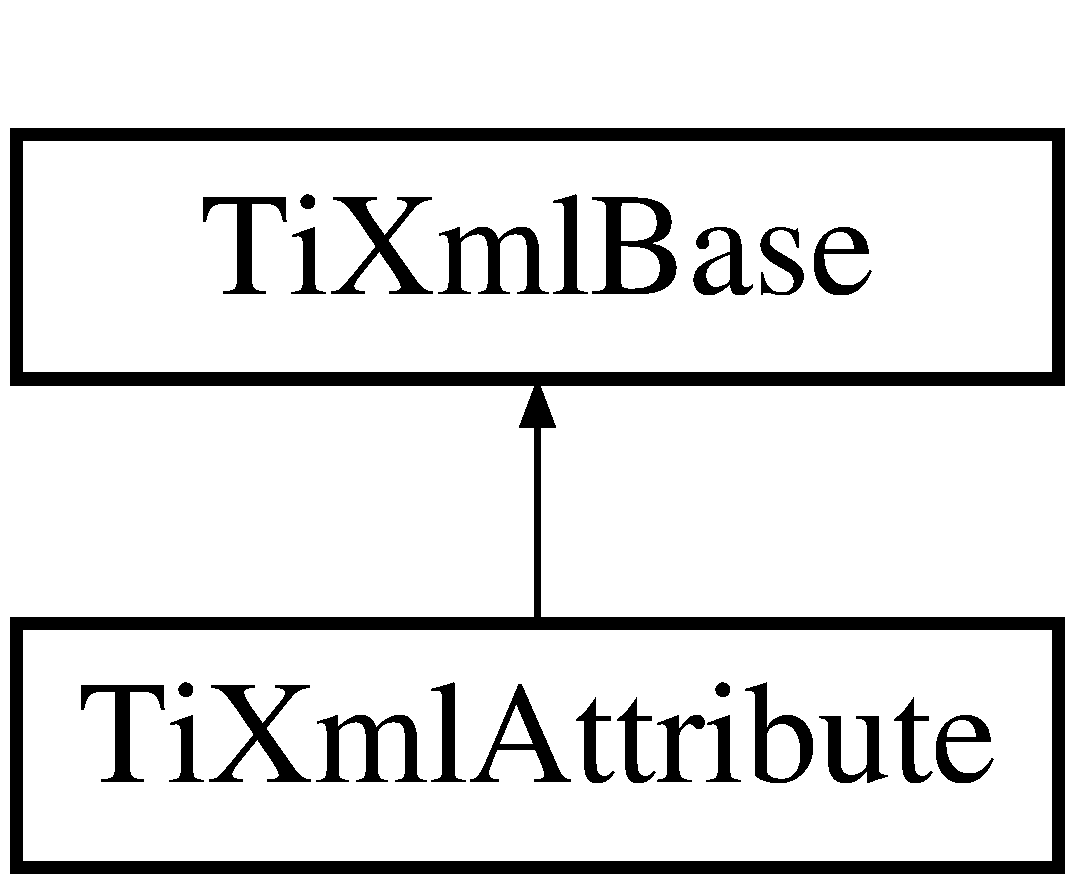
\includegraphics[height=2cm]{classTiXmlAttribute}
\end{center}
\end{figure}


\subsection{Detailed Description}
An attribute is a name-value pair. Elements have an arbitrary number of attributes, each with a unique name.

\begin{Desc}
\item[Note:]The attributes are not TiXmlNodes, since they are not part of the tinyXML document object \doxyref{model}{p.}{structmodel}. There are other suggested ways to look at this problem. \end{Desc}
\subsection*{Public Member Functions}
\begin{CompactItemize}
\item 
{\bf TiXmlAttribute} ()
\begin{CompactList}\small\item\em Construct an empty attribute. \item\end{CompactList}\item 
{\bf TiXmlAttribute} (const char $\ast$\_\-name, const char $\ast$\_\-value)
\begin{CompactList}\small\item\em Construct an attribute with a name and value. \item\end{CompactList}\item 
const char $\ast$ {\bf Name} () const 
\begin{CompactList}\small\item\em Return the name of this attribute. \item\end{CompactList}\item 
const char $\ast$ {\bf Value} () const 
\begin{CompactList}\small\item\em Return the value of this attribute. \item\end{CompactList}\item 
int {\bf IntValue} () const 
\begin{CompactList}\small\item\em Return the value of this attribute, converted to an integer. \item\end{CompactList}\item 
double {\bf DoubleValue} () const 
\begin{CompactList}\small\item\em Return the value of this attribute, converted to a double. \item\end{CompactList}\item 
const TIXML\_\-STRING \& {\bf NameTStr} () const 
\item 
int {\bf QueryIntValue} (int $\ast$\_\-value) const 
\item 
int {\bf QueryDoubleValue} (double $\ast$\_\-value) const 
\begin{CompactList}\small\item\em QueryDoubleValue examines the value string. See \doxyref{QueryIntValue()}{p.}{classTiXmlAttribute_d6c93088ee21af41a107931223339344}. \item\end{CompactList}\item 
void {\bf SetName} (const char $\ast$\_\-name)
\begin{CompactList}\small\item\em Set the name of this attribute. \item\end{CompactList}\item 
void {\bf SetValue} (const char $\ast$\_\-value)
\begin{CompactList}\small\item\em Set the value. \item\end{CompactList}\item 
void {\bf SetIntValue} (int \_\-value)
\begin{CompactList}\small\item\em Set the value from an integer. \item\end{CompactList}\item 
void {\bf SetDoubleValue} (double \_\-value)
\begin{CompactList}\small\item\em Set the value from a double. \item\end{CompactList}\item 
const {\bf TiXmlAttribute} $\ast$ {\bf Next} () const 
\begin{CompactList}\small\item\em Get the next sibling attribute in the DOM. Returns null at end. \item\end{CompactList}\item 
{\bf TiXmlAttribute} $\ast$ {\bf Next} ()
\item 
const {\bf TiXmlAttribute} $\ast$ {\bf Previous} () const 
\begin{CompactList}\small\item\em Get the previous sibling attribute in the DOM. Returns null at beginning. \item\end{CompactList}\item 
{\bf TiXmlAttribute} $\ast$ {\bf Previous} ()
\item 
bool {\bf operator==} (const {\bf TiXmlAttribute} \&rhs) const 
\item 
bool {\bf operator$<$} (const {\bf TiXmlAttribute} \&rhs) const 
\item 
bool {\bf operator$>$} (const {\bf TiXmlAttribute} \&rhs) const 
\item 
virtual const char $\ast$ {\bf Parse} (const char $\ast$p, {\bf TiXmlParsingData} $\ast$data, {\bf TiXmlEncoding} encoding)
\item 
virtual void {\bf Print} (FILE $\ast$cfile, int depth) const 
\item 
void {\bf Print} (FILE $\ast$cfile, int depth, TIXML\_\-STRING $\ast$str) const 
\item 
void {\bf SetDocument} ({\bf TiXmlDocument} $\ast$doc)
\end{CompactItemize}
\subsection*{Friends}
\begin{CompactItemize}
\item 
class {\bf TiXmlAttributeSet}
\end{CompactItemize}


\subsection{Constructor \& Destructor Documentation}
\index{TiXmlAttribute@{TiXmlAttribute}!TiXmlAttribute@{TiXmlAttribute}}
\index{TiXmlAttribute@{TiXmlAttribute}!TiXmlAttribute@{TiXmlAttribute}}
\subsubsection{\setlength{\rightskip}{0pt plus 5cm}TiXmlAttribute::TiXmlAttribute ()\hspace{0.3cm}{\tt  [inline]}}\label{classTiXmlAttribute_9cfa3c8179873fd485d83003b114f8e1}


Construct an empty attribute. 

\index{TiXmlAttribute@{TiXmlAttribute}!TiXmlAttribute@{TiXmlAttribute}}
\index{TiXmlAttribute@{TiXmlAttribute}!TiXmlAttribute@{TiXmlAttribute}}
\subsubsection{\setlength{\rightskip}{0pt plus 5cm}TiXmlAttribute::TiXmlAttribute (const char $\ast$ {\em \_\-name}, const char $\ast$ {\em \_\-value})\hspace{0.3cm}{\tt  [inline]}}\label{classTiXmlAttribute_759d0b76fb8fcf765ecab243bc14f05e}


Construct an attribute with a name and value. 



\subsection{Member Function Documentation}
\index{TiXmlAttribute@{TiXmlAttribute}!Name@{Name}}
\index{Name@{Name}!TiXmlAttribute@{TiXmlAttribute}}
\subsubsection{\setlength{\rightskip}{0pt plus 5cm}const char$\ast$ TiXmlAttribute::Name () const\hspace{0.3cm}{\tt  [inline]}}\label{classTiXmlAttribute_298a57287d305904ba6bd96ae6f78d3d}


Return the name of this attribute. 

\index{TiXmlAttribute@{TiXmlAttribute}!Value@{Value}}
\index{Value@{Value}!TiXmlAttribute@{TiXmlAttribute}}
\subsubsection{\setlength{\rightskip}{0pt plus 5cm}const char$\ast$ TiXmlAttribute::Value () const\hspace{0.3cm}{\tt  [inline]}}\label{classTiXmlAttribute_0f874490eac8ca00ee0070765d0e97e3}


Return the value of this attribute. 

\index{TiXmlAttribute@{TiXmlAttribute}!IntValue@{IntValue}}
\index{IntValue@{IntValue}!TiXmlAttribute@{TiXmlAttribute}}
\subsubsection{\setlength{\rightskip}{0pt plus 5cm}int TiXmlAttribute::IntValue () const}\label{classTiXmlAttribute_a1a20ad59dc7e89a0ab265396360d50f}


Return the value of this attribute, converted to an integer. 

\index{TiXmlAttribute@{TiXmlAttribute}!DoubleValue@{DoubleValue}}
\index{DoubleValue@{DoubleValue}!TiXmlAttribute@{TiXmlAttribute}}
\subsubsection{\setlength{\rightskip}{0pt plus 5cm}double TiXmlAttribute::DoubleValue () const}\label{classTiXmlAttribute_2880ddef53fc7522c99535273954d230}


Return the value of this attribute, converted to a double. 

\index{TiXmlAttribute@{TiXmlAttribute}!NameTStr@{NameTStr}}
\index{NameTStr@{NameTStr}!TiXmlAttribute@{TiXmlAttribute}}
\subsubsection{\setlength{\rightskip}{0pt plus 5cm}const TIXML\_\-STRING\& TiXmlAttribute::NameTStr () const\hspace{0.3cm}{\tt  [inline]}}\label{classTiXmlAttribute_64cee17bceb8232eb0736d26dd082d79}


\index{TiXmlAttribute@{TiXmlAttribute}!QueryIntValue@{QueryIntValue}}
\index{QueryIntValue@{QueryIntValue}!TiXmlAttribute@{TiXmlAttribute}}
\subsubsection{\setlength{\rightskip}{0pt plus 5cm}int TiXmlAttribute::QueryIntValue (int $\ast$ {\em \_\-value}) const}\label{classTiXmlAttribute_d6c93088ee21af41a107931223339344}


QueryIntValue examines the value string. It is an alternative to the \doxyref{IntValue()}{p.}{classTiXmlAttribute_a1a20ad59dc7e89a0ab265396360d50f} method with richer error checking. If the value is an integer, it is stored in 'value' and the call returns TIXML\_\-SUCCESS. If it is not an integer, it returns TIXML\_\-WRONG\_\-TYPE.

A specialized but useful call. Note that for success it returns 0, which is the opposite of almost all other TinyXml calls. \index{TiXmlAttribute@{TiXmlAttribute}!QueryDoubleValue@{QueryDoubleValue}}
\index{QueryDoubleValue@{QueryDoubleValue}!TiXmlAttribute@{TiXmlAttribute}}
\subsubsection{\setlength{\rightskip}{0pt plus 5cm}int TiXmlAttribute::QueryDoubleValue (double $\ast$ {\em \_\-value}) const}\label{classTiXmlAttribute_c87b2a8489906a5d7aa2875f20be3513}


QueryDoubleValue examines the value string. See \doxyref{QueryIntValue()}{p.}{classTiXmlAttribute_d6c93088ee21af41a107931223339344}. 

\index{TiXmlAttribute@{TiXmlAttribute}!SetName@{SetName}}
\index{SetName@{SetName}!TiXmlAttribute@{TiXmlAttribute}}
\subsubsection{\setlength{\rightskip}{0pt plus 5cm}void TiXmlAttribute::SetName (const char $\ast$ {\em \_\-name})\hspace{0.3cm}{\tt  [inline]}}\label{classTiXmlAttribute_b7fa3d21ff8d7c5764cf9af15b667a99}


Set the name of this attribute. 

\index{TiXmlAttribute@{TiXmlAttribute}!SetValue@{SetValue}}
\index{SetValue@{SetValue}!TiXmlAttribute@{TiXmlAttribute}}
\subsubsection{\setlength{\rightskip}{0pt plus 5cm}void TiXmlAttribute::SetValue (const char $\ast$ {\em \_\-value})\hspace{0.3cm}{\tt  [inline]}}\label{classTiXmlAttribute_2dae44178f668b3cb48101be4f2236a0}


Set the value. 

\index{TiXmlAttribute@{TiXmlAttribute}!SetIntValue@{SetIntValue}}
\index{SetIntValue@{SetIntValue}!TiXmlAttribute@{TiXmlAttribute}}
\subsubsection{\setlength{\rightskip}{0pt plus 5cm}void TiXmlAttribute::SetIntValue (int {\em \_\-value})}\label{classTiXmlAttribute_7e065df640116a62ea4f4b7da5449cc8}


Set the value from an integer. 

\index{TiXmlAttribute@{TiXmlAttribute}!SetDoubleValue@{SetDoubleValue}}
\index{SetDoubleValue@{SetDoubleValue}!TiXmlAttribute@{TiXmlAttribute}}
\subsubsection{\setlength{\rightskip}{0pt plus 5cm}void TiXmlAttribute::SetDoubleValue (double {\em \_\-value})}\label{classTiXmlAttribute_0316da31373496c4368ad549bf711394}


Set the value from a double. 

\index{TiXmlAttribute@{TiXmlAttribute}!Next@{Next}}
\index{Next@{Next}!TiXmlAttribute@{TiXmlAttribute}}
\subsubsection{\setlength{\rightskip}{0pt plus 5cm}const {\bf TiXmlAttribute} $\ast$ TiXmlAttribute::Next () const}\label{classTiXmlAttribute_776478980776a024f7c2846eec640f65}


Get the next sibling attribute in the DOM. Returns null at end. 

\index{TiXmlAttribute@{TiXmlAttribute}!Next@{Next}}
\index{Next@{Next}!TiXmlAttribute@{TiXmlAttribute}}
\subsubsection{\setlength{\rightskip}{0pt plus 5cm}{\bf TiXmlAttribute}$\ast$ TiXmlAttribute::Next ()\hspace{0.3cm}{\tt  [inline]}}\label{classTiXmlAttribute_138320aa7793b148ba7e5bd0a0ea4db6}


\index{TiXmlAttribute@{TiXmlAttribute}!Previous@{Previous}}
\index{Previous@{Previous}!TiXmlAttribute@{TiXmlAttribute}}
\subsubsection{\setlength{\rightskip}{0pt plus 5cm}const {\bf TiXmlAttribute} $\ast$ TiXmlAttribute::Previous () const}\label{classTiXmlAttribute_54a5f8730c7b02b9a41b74e12e27fe86}


Get the previous sibling attribute in the DOM. Returns null at beginning. 

\index{TiXmlAttribute@{TiXmlAttribute}!Previous@{Previous}}
\index{Previous@{Previous}!TiXmlAttribute@{TiXmlAttribute}}
\subsubsection{\setlength{\rightskip}{0pt plus 5cm}{\bf TiXmlAttribute}$\ast$ TiXmlAttribute::Previous ()\hspace{0.3cm}{\tt  [inline]}}\label{classTiXmlAttribute_e4dabc932cba945ed1e92fec5f121193}


\index{TiXmlAttribute@{TiXmlAttribute}!operator==@{operator==}}
\index{operator==@{operator==}!TiXmlAttribute@{TiXmlAttribute}}
\subsubsection{\setlength{\rightskip}{0pt plus 5cm}bool TiXmlAttribute::operator== (const {\bf TiXmlAttribute} \& {\em rhs}) const\hspace{0.3cm}{\tt  [inline]}}\label{classTiXmlAttribute_e48c2a65b520d453914ce4e845d607cf}


\index{TiXmlAttribute@{TiXmlAttribute}!operator$<$@{operator$<$}}
\index{operator$<$@{operator$<$}!TiXmlAttribute@{TiXmlAttribute}}
\subsubsection{\setlength{\rightskip}{0pt plus 5cm}bool TiXmlAttribute::operator$<$ (const {\bf TiXmlAttribute} \& {\em rhs}) const\hspace{0.3cm}{\tt  [inline]}}\label{classTiXmlAttribute_db8b6f2cad5948e73e383182e7ce10de}


\index{TiXmlAttribute@{TiXmlAttribute}!operator$>$@{operator$>$}}
\index{operator$>$@{operator$>$}!TiXmlAttribute@{TiXmlAttribute}}
\subsubsection{\setlength{\rightskip}{0pt plus 5cm}bool TiXmlAttribute::operator$>$ (const {\bf TiXmlAttribute} \& {\em rhs}) const\hspace{0.3cm}{\tt  [inline]}}\label{classTiXmlAttribute_867562769ef9778c1690cd373246b05b}


\index{TiXmlAttribute@{TiXmlAttribute}!Parse@{Parse}}
\index{Parse@{Parse}!TiXmlAttribute@{TiXmlAttribute}}
\subsubsection{\setlength{\rightskip}{0pt plus 5cm}const char $\ast$ TiXmlAttribute::Parse (const char $\ast$ {\em p}, {\bf TiXmlParsingData} $\ast$ {\em data}, {\bf TiXmlEncoding} {\em encoding})\hspace{0.3cm}{\tt  [virtual]}}\label{classTiXmlAttribute_d62774421b814894b995af3b5d231dda}




Implements {\bf TiXmlBase} \doxyref{}{p.}{classTiXmlBase_00e4edb0219d00a1379c856e5a1d2025}.\index{TiXmlAttribute@{TiXmlAttribute}!Print@{Print}}
\index{Print@{Print}!TiXmlAttribute@{TiXmlAttribute}}
\subsubsection{\setlength{\rightskip}{0pt plus 5cm}virtual void TiXmlAttribute::Print (FILE $\ast$ {\em cfile}, int {\em depth}) const\hspace{0.3cm}{\tt  [inline, virtual]}}\label{classTiXmlAttribute_cc04956c1d5c4c31fe74f7a7528d109a}


All TinyXml classes can print themselves to a filestream or the string class (\doxyref{TiXmlString}{p.}{classTiXmlString} in non-STL mode, std::string in STL mode.) Either or both cfile and str can be null.

This is a formatted print, and will insert tabs and newlines.

(For an unformatted stream, use the $<$$<$ operator.) 

Implements {\bf TiXmlBase} \doxyref{}{p.}{classTiXmlBase_0de56b3f2ef14c65091a3b916437b512}.\index{TiXmlAttribute@{TiXmlAttribute}!Print@{Print}}
\index{Print@{Print}!TiXmlAttribute@{TiXmlAttribute}}
\subsubsection{\setlength{\rightskip}{0pt plus 5cm}void TiXmlAttribute::Print (FILE $\ast$ {\em cfile}, int {\em depth}, TIXML\_\-STRING $\ast$ {\em str}) const}\label{classTiXmlAttribute_19e6b6862a80b188571c47947e88d030}


\index{TiXmlAttribute@{TiXmlAttribute}!SetDocument@{SetDocument}}
\index{SetDocument@{SetDocument}!TiXmlAttribute@{TiXmlAttribute}}
\subsubsection{\setlength{\rightskip}{0pt plus 5cm}void TiXmlAttribute::SetDocument ({\bf TiXmlDocument} $\ast$ {\em doc})\hspace{0.3cm}{\tt  [inline]}}\label{classTiXmlAttribute_c12a94d4548302afb12f488ba101f7d1}




\subsection{Friends And Related Function Documentation}
\index{TiXmlAttribute@{TiXmlAttribute}!TiXmlAttributeSet@{TiXmlAttributeSet}}
\index{TiXmlAttributeSet@{TiXmlAttributeSet}!TiXmlAttribute@{TiXmlAttribute}}
\subsubsection{\setlength{\rightskip}{0pt plus 5cm}friend class {\bf TiXmlAttributeSet}\hspace{0.3cm}{\tt  [friend]}}\label{classTiXmlAttribute_35a7b7f89f708527677d5078d41ce0bf}




The documentation for this class was generated from the following files:\begin{CompactItemize}
\item 
/home/msneddon/eclipse/indigo/workspace/NFsim/src/NFinput/TinyXML/{\bf tinyxml.h}\item 
/home/msneddon/eclipse/indigo/workspace/NFsim/src/NFinput/TinyXML/{\bf tinyxml.cpp}\item 
/home/msneddon/eclipse/indigo/workspace/NFsim/src/NFinput/TinyXML/{\bf tinyxmlparser.cpp}\end{CompactItemize}

\section{TiXmlAttributeSet Class Reference}
\label{classTiXmlAttributeSet}\index{TiXmlAttributeSet@{TiXmlAttributeSet}}
{\tt \#include $<$tinyxml.h$>$}



\subsection{Detailed Description}
A class used to manage a group of attributes. It is only used internally, both by the ELEMENT and the DECLARATION.

The set can be changed transparent to the Element and Declaration classes that use it, but NOT transparent to the Attribute which has to implement a next() and previous() method. Which makes it a bit problematic and prevents the use of STL.

This version is implemented with circular lists because:\begin{itemize}
\item I like circular lists\item it demonstrates some independence from the (typical) doubly linked list. \end{itemize}
\subsection*{Public Member Functions}
\begin{CompactItemize}
\item 
{\bf TiXmlAttributeSet} ()
\item 
{\bf $\sim$TiXmlAttributeSet} ()
\item 
void {\bf Add} ({\bf TiXmlAttribute} $\ast$attribute)
\item 
void {\bf Remove} ({\bf TiXmlAttribute} $\ast$attribute)
\item 
const {\bf TiXmlAttribute} $\ast$ {\bf First} () const 
\item 
{\bf TiXmlAttribute} $\ast$ {\bf First} ()
\item 
const {\bf TiXmlAttribute} $\ast$ {\bf Last} () const 
\item 
{\bf TiXmlAttribute} $\ast$ {\bf Last} ()
\item 
const {\bf TiXmlAttribute} $\ast$ {\bf Find} (const char $\ast$\_\-name) const 
\item 
{\bf TiXmlAttribute} $\ast$ {\bf Find} (const char $\ast$\_\-name)
\end{CompactItemize}


\subsection{Constructor \& Destructor Documentation}
\index{TiXmlAttributeSet@{TiXmlAttributeSet}!TiXmlAttributeSet@{TiXmlAttributeSet}}
\index{TiXmlAttributeSet@{TiXmlAttributeSet}!TiXmlAttributeSet@{TiXmlAttributeSet}}
\subsubsection{\setlength{\rightskip}{0pt plus 5cm}TiXmlAttributeSet::TiXmlAttributeSet ()}\label{classTiXmlAttributeSet_253c33b657cc85a07f7f060b02146c35}


\index{TiXmlAttributeSet@{TiXmlAttributeSet}!$\sim$TiXmlAttributeSet@{$\sim$TiXmlAttributeSet}}
\index{$\sim$TiXmlAttributeSet@{$\sim$TiXmlAttributeSet}!TiXmlAttributeSet@{TiXmlAttributeSet}}
\subsubsection{\setlength{\rightskip}{0pt plus 5cm}TiXmlAttributeSet::$\sim$TiXmlAttributeSet ()}\label{classTiXmlAttributeSet_dd463905dff96142a29fe16a01ecf28f}




\subsection{Member Function Documentation}
\index{TiXmlAttributeSet@{TiXmlAttributeSet}!Add@{Add}}
\index{Add@{Add}!TiXmlAttributeSet@{TiXmlAttributeSet}}
\subsubsection{\setlength{\rightskip}{0pt plus 5cm}void TiXmlAttributeSet::Add ({\bf TiXmlAttribute} $\ast$ {\em attribute})}\label{classTiXmlAttributeSet_745e50ddaae3bee93e4589321e0b9c1a}


\index{TiXmlAttributeSet@{TiXmlAttributeSet}!Remove@{Remove}}
\index{Remove@{Remove}!TiXmlAttributeSet@{TiXmlAttributeSet}}
\subsubsection{\setlength{\rightskip}{0pt plus 5cm}void TiXmlAttributeSet::Remove ({\bf TiXmlAttribute} $\ast$ {\em attribute})}\label{classTiXmlAttributeSet_924a73d071f2573f9060f0be57879c57}


\index{TiXmlAttributeSet@{TiXmlAttributeSet}!First@{First}}
\index{First@{First}!TiXmlAttributeSet@{TiXmlAttributeSet}}
\subsubsection{\setlength{\rightskip}{0pt plus 5cm}const {\bf TiXmlAttribute}$\ast$ TiXmlAttributeSet::First () const\hspace{0.3cm}{\tt  [inline]}}\label{classTiXmlAttributeSet_e0636e88cedd4b09d61c451860f68598}


\index{TiXmlAttributeSet@{TiXmlAttributeSet}!First@{First}}
\index{First@{First}!TiXmlAttributeSet@{TiXmlAttributeSet}}
\subsubsection{\setlength{\rightskip}{0pt plus 5cm}{\bf TiXmlAttribute}$\ast$ TiXmlAttributeSet::First ()\hspace{0.3cm}{\tt  [inline]}}\label{classTiXmlAttributeSet_99703bb08ca2aece2d7ef835de339ba0}


\index{TiXmlAttributeSet@{TiXmlAttributeSet}!Last@{Last}}
\index{Last@{Last}!TiXmlAttributeSet@{TiXmlAttributeSet}}
\subsubsection{\setlength{\rightskip}{0pt plus 5cm}const {\bf TiXmlAttribute}$\ast$ TiXmlAttributeSet::Last () const\hspace{0.3cm}{\tt  [inline]}}\label{classTiXmlAttributeSet_7b3f3ccf39a97bc25539d3fcc540296a}


\index{TiXmlAttributeSet@{TiXmlAttributeSet}!Last@{Last}}
\index{Last@{Last}!TiXmlAttributeSet@{TiXmlAttributeSet}}
\subsubsection{\setlength{\rightskip}{0pt plus 5cm}{\bf TiXmlAttribute}$\ast$ TiXmlAttributeSet::Last ()\hspace{0.3cm}{\tt  [inline]}}\label{classTiXmlAttributeSet_b4c4edfb2d74f6ea31aae096743bd6e0}


\index{TiXmlAttributeSet@{TiXmlAttributeSet}!Find@{Find}}
\index{Find@{Find}!TiXmlAttributeSet@{TiXmlAttributeSet}}
\subsubsection{\setlength{\rightskip}{0pt plus 5cm}const {\bf TiXmlAttribute} $\ast$ TiXmlAttributeSet::Find (const char $\ast$ {\em \_\-name}) const}\label{classTiXmlAttributeSet_acbbc5e1a1c987e72815430e89fcb58b}


\index{TiXmlAttributeSet@{TiXmlAttributeSet}!Find@{Find}}
\index{Find@{Find}!TiXmlAttributeSet@{TiXmlAttributeSet}}
\subsubsection{\setlength{\rightskip}{0pt plus 5cm}{\bf TiXmlAttribute}$\ast$ TiXmlAttributeSet::Find (const char $\ast$ {\em \_\-name})\hspace{0.3cm}{\tt  [inline]}}\label{classTiXmlAttributeSet_2f210bed54c832adf1683c44c35727b9}




The documentation for this class was generated from the following files:\begin{CompactItemize}
\item 
/home/msneddon/eclipse/ganymede\_\-cpp/workspace/NFsim\_\-svn/src/NFinput/TinyXML/{\bf tinyxml.h}\item 
/home/msneddon/eclipse/ganymede\_\-cpp/workspace/NFsim\_\-svn/src/NFinput/TinyXML/{\bf tinyxml.cpp}\end{CompactItemize}

\section{TiXmlBase Class Reference}
\label{classTiXmlBase}\index{TiXmlBase@{TiXmlBase}}
{\tt \#include $<$tinyxml.h$>$}

Inheritance diagram for TiXmlBase::\begin{figure}[H]
\begin{center}
\leavevmode
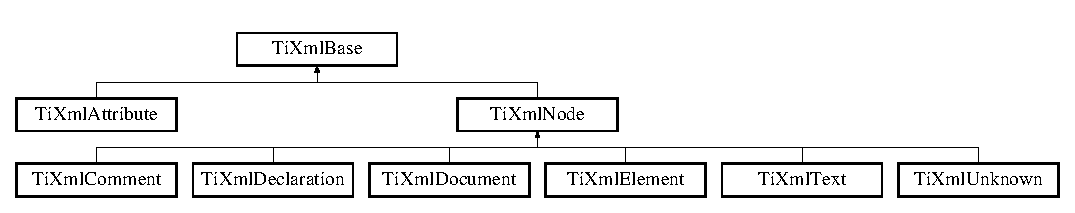
\includegraphics[height=2.41379cm]{classTiXmlBase}
\end{center}
\end{figure}


\subsection{Detailed Description}
\doxyref{TiXmlBase}{p.}{classTiXmlBase} is a base class for every class in TinyXml. It does little except to establish that TinyXml classes can be printed and provide some utility functions.

In XML, the document and elements can contain other elements and other types of nodes.



\footnotesize\begin{verbatim}
	A Document can contain:	Element	(container or leaf)
							Comment (leaf)
							Unknown (leaf)
							Declaration( leaf )

	An Element can contain:	Element (container or leaf)
							Text	(leaf)
							Attributes (not on tree)
							Comment (leaf)
							Unknown (leaf)

	A Decleration contains: Attributes (not on tree)
	\end{verbatim}
\normalsize
 \subsection*{Public Types}
\begin{CompactItemize}
\item 
enum \{ \par
{\bf TIXML\_\-NO\_\-ERROR} =  0, 
{\bf TIXML\_\-ERROR}, 
{\bf TIXML\_\-ERROR\_\-OPENING\_\-FILE}, 
{\bf TIXML\_\-ERROR\_\-OUT\_\-OF\_\-MEMORY}, 
\par
{\bf TIXML\_\-ERROR\_\-PARSING\_\-ELEMENT}, 
{\bf TIXML\_\-ERROR\_\-FAILED\_\-TO\_\-READ\_\-ELEMENT\_\-NAME}, 
{\bf TIXML\_\-ERROR\_\-READING\_\-ELEMENT\_\-VALUE}, 
{\bf TIXML\_\-ERROR\_\-READING\_\-ATTRIBUTES}, 
\par
{\bf TIXML\_\-ERROR\_\-PARSING\_\-EMPTY}, 
{\bf TIXML\_\-ERROR\_\-READING\_\-END\_\-TAG}, 
{\bf TIXML\_\-ERROR\_\-PARSING\_\-UNKNOWN}, 
{\bf TIXML\_\-ERROR\_\-PARSING\_\-COMMENT}, 
\par
{\bf TIXML\_\-ERROR\_\-PARSING\_\-DECLARATION}, 
{\bf TIXML\_\-ERROR\_\-DOCUMENT\_\-EMPTY}, 
{\bf TIXML\_\-ERROR\_\-EMBEDDED\_\-NULL}, 
{\bf TIXML\_\-ERROR\_\-PARSING\_\-CDATA}, 
\par
{\bf TIXML\_\-ERROR\_\-DOCUMENT\_\-TOP\_\-ONLY}, 
{\bf TIXML\_\-ERROR\_\-STRING\_\-COUNT}
 \}
\end{CompactItemize}
\subsection*{Public Member Functions}
\begin{CompactItemize}
\item 
{\bf TiXmlBase} ()
\item 
virtual {\bf $\sim$TiXmlBase} ()
\item 
virtual void {\bf Print} (FILE $\ast$cfile, int depth) const =0
\item 
int {\bf Row} () const 
\item 
int {\bf Column} () const 
\begin{CompactList}\small\item\em See \doxyref{Row()}{p.}{classTiXmlBase_024bceb070188df92c2a8d8852dd0853}. \item\end{CompactList}\item 
void {\bf SetUserData} (void $\ast$user)
\begin{CompactList}\small\item\em Set a pointer to arbitrary user data. \item\end{CompactList}\item 
void $\ast$ {\bf GetUserData} ()
\begin{CompactList}\small\item\em Get a pointer to arbitrary user data. \item\end{CompactList}\item 
const void $\ast$ {\bf GetUserData} () const 
\begin{CompactList}\small\item\em Get a pointer to arbitrary user data. \item\end{CompactList}\item 
virtual const char $\ast$ {\bf Parse} (const char $\ast$p, {\bf TiXmlParsingData} $\ast$data, {\bf TiXmlEncoding} encoding)=0
\end{CompactItemize}
\subsection*{Static Public Member Functions}
\begin{CompactItemize}
\item 
static void {\bf SetCondenseWhiteSpace} (bool condense)
\item 
static bool {\bf IsWhiteSpaceCondensed} ()
\begin{CompactList}\small\item\em Return the current white space setting. \item\end{CompactList}\item 
static void {\bf EncodeString} (const TIXML\_\-STRING \&str, TIXML\_\-STRING $\ast$out)
\end{CompactItemize}
\subsection*{Static Public Attributes}
\begin{CompactItemize}
\item 
static const int {\bf utf8ByteTable} [256]
\end{CompactItemize}
\subsection*{Static Protected Member Functions}
\begin{CompactItemize}
\item 
static const char $\ast$ {\bf SkipWhiteSpace} (const char $\ast$, {\bf TiXmlEncoding} encoding)
\item 
static bool {\bf IsWhiteSpace} (char c)
\item 
static bool {\bf IsWhiteSpace} (int c)
\item 
static const char $\ast$ {\bf ReadName} (const char $\ast$p, TIXML\_\-STRING $\ast$name, {\bf TiXmlEncoding} encoding)
\item 
static const char $\ast$ {\bf ReadText} (const char $\ast$in, TIXML\_\-STRING $\ast$text, bool ignoreWhiteSpace, const char $\ast$endTag, bool ignoreCase, {\bf TiXmlEncoding} encoding)
\item 
static const char $\ast$ {\bf GetEntity} (const char $\ast$in, char $\ast$value, int $\ast$length, {\bf TiXmlEncoding} encoding)
\item 
static const char $\ast$ {\bf GetChar} (const char $\ast$p, char $\ast$\_\-value, int $\ast$length, {\bf TiXmlEncoding} encoding)
\item 
static bool {\bf StringEqual} (const char $\ast$p, const char $\ast$endTag, bool ignoreCase, {\bf TiXmlEncoding} encoding)
\item 
static int {\bf IsAlpha} (unsigned char anyByte, {\bf TiXmlEncoding} encoding)
\item 
static int {\bf IsAlphaNum} (unsigned char anyByte, {\bf TiXmlEncoding} encoding)
\item 
static int {\bf ToLower} (int v, {\bf TiXmlEncoding} encoding)
\item 
static void {\bf ConvertUTF32ToUTF8} (unsigned long input, char $\ast$output, int $\ast$length)
\end{CompactItemize}
\subsection*{Protected Attributes}
\begin{CompactItemize}
\item 
{\bf TiXmlCursor} {\bf location}
\item 
void $\ast$ {\bf userData}
\begin{CompactList}\small\item\em Field containing a generic user pointer. \item\end{CompactList}\end{CompactItemize}
\subsection*{Static Protected Attributes}
\begin{CompactItemize}
\item 
static const char $\ast$ {\bf errorString} [TIXML\_\-ERROR\_\-STRING\_\-COUNT]
\end{CompactItemize}
\subsection*{Friends}
\begin{CompactItemize}
\item 
class {\bf TiXmlNode}
\item 
class {\bf TiXmlElement}
\item 
class {\bf TiXmlDocument}
\end{CompactItemize}
\subsection*{Classes}
\begin{CompactItemize}
\item 
struct \textbf{Entity}
\end{CompactItemize}


\subsection{Member Enumeration Documentation}
\subsubsection{\setlength{\rightskip}{0pt plus 5cm}anonymous enum}\label{classTiXmlBase_9a7e9344415956ab96e8c75f6a0bbd48}


\begin{Desc}
\item[Enumerator: ]\par
\begin{description}
\index{TIXML\_\-NO\_\-ERROR@{TIXML\_\-NO\_\-ERROR}!TiXmlBase@{TiXmlBase}}\index{TiXmlBase@{TiXmlBase}!TIXML\_\-NO\_\-ERROR@{TIXML\_\-NO\_\-ERROR}}\item[{\em 
TIXML\_\-NO\_\-ERROR\label{classTiXmlBase_9a7e9344415956ab96e8c75f6a0bbd48750a76ca602241c416d5ec357d55fba1}
}]\index{TIXML\_\-ERROR@{TIXML\_\-ERROR}!TiXmlBase@{TiXmlBase}}\index{TiXmlBase@{TiXmlBase}!TIXML\_\-ERROR@{TIXML\_\-ERROR}}\item[{\em 
TIXML\_\-ERROR\label{classTiXmlBase_9a7e9344415956ab96e8c75f6a0bbd48bcabc1b8efabeda1cc4352aa73d64390}
}]\index{TIXML\_\-ERROR\_\-OPENING\_\-FILE@{TIXML\_\-ERROR\_\-OPENING\_\-FILE}!TiXmlBase@{TiXmlBase}}\index{TiXmlBase@{TiXmlBase}!TIXML\_\-ERROR\_\-OPENING\_\-FILE@{TIXML\_\-ERROR\_\-OPENING\_\-FILE}}\item[{\em 
TIXML\_\-ERROR\_\-OPENING\_\-FILE\label{classTiXmlBase_9a7e9344415956ab96e8c75f6a0bbd48b803949b8f12e03b5b57f86d9c52b614}
}]\index{TIXML\_\-ERROR\_\-OUT\_\-OF\_\-MEMORY@{TIXML\_\-ERROR\_\-OUT\_\-OF\_\-MEMORY}!TiXmlBase@{TiXmlBase}}\index{TiXmlBase@{TiXmlBase}!TIXML\_\-ERROR\_\-OUT\_\-OF\_\-MEMORY@{TIXML\_\-ERROR\_\-OUT\_\-OF\_\-MEMORY}}\item[{\em 
TIXML\_\-ERROR\_\-OUT\_\-OF\_\-MEMORY\label{classTiXmlBase_9a7e9344415956ab96e8c75f6a0bbd4892e3bfc96126d3544f47e8b3f031e7bb}
}]\index{TIXML\_\-ERROR\_\-PARSING\_\-ELEMENT@{TIXML\_\-ERROR\_\-PARSING\_\-ELEMENT}!TiXmlBase@{TiXmlBase}}\index{TiXmlBase@{TiXmlBase}!TIXML\_\-ERROR\_\-PARSING\_\-ELEMENT@{TIXML\_\-ERROR\_\-PARSING\_\-ELEMENT}}\item[{\em 
TIXML\_\-ERROR\_\-PARSING\_\-ELEMENT\label{classTiXmlBase_9a7e9344415956ab96e8c75f6a0bbd485cbfcf7fe5e67f0cd1aef98deac55dd2}
}]\index{TIXML\_\-ERROR\_\-FAILED\_\-TO\_\-READ\_\-ELEMENT\_\-NAME@{TIXML\_\-ERROR\_\-FAILED\_\-TO\_\-READ\_\-ELEMENT\_\-NAME}!TiXmlBase@{TiXmlBase}}\index{TiXmlBase@{TiXmlBase}!TIXML\_\-ERROR\_\-FAILED\_\-TO\_\-READ\_\-ELEMENT\_\-NAME@{TIXML\_\-ERROR\_\-FAILED\_\-TO\_\-READ\_\-ELEMENT\_\-NAME}}\item[{\em 
TIXML\_\-ERROR\_\-FAILED\_\-TO\_\-READ\_\-ELEMENT\_\-NAME\label{classTiXmlBase_9a7e9344415956ab96e8c75f6a0bbd48dcc31ca78a9d507a88c9fafb3d18a3c4}
}]\index{TIXML\_\-ERROR\_\-READING\_\-ELEMENT\_\-VALUE@{TIXML\_\-ERROR\_\-READING\_\-ELEMENT\_\-VALUE}!TiXmlBase@{TiXmlBase}}\index{TiXmlBase@{TiXmlBase}!TIXML\_\-ERROR\_\-READING\_\-ELEMENT\_\-VALUE@{TIXML\_\-ERROR\_\-READING\_\-ELEMENT\_\-VALUE}}\item[{\em 
TIXML\_\-ERROR\_\-READING\_\-ELEMENT\_\-VALUE\label{classTiXmlBase_9a7e9344415956ab96e8c75f6a0bbd48fefdc75db23215e846605a2b5af0c2d3}
}]\index{TIXML\_\-ERROR\_\-READING\_\-ATTRIBUTES@{TIXML\_\-ERROR\_\-READING\_\-ATTRIBUTES}!TiXmlBase@{TiXmlBase}}\index{TiXmlBase@{TiXmlBase}!TIXML\_\-ERROR\_\-READING\_\-ATTRIBUTES@{TIXML\_\-ERROR\_\-READING\_\-ATTRIBUTES}}\item[{\em 
TIXML\_\-ERROR\_\-READING\_\-ATTRIBUTES\label{classTiXmlBase_9a7e9344415956ab96e8c75f6a0bbd48670fac23171b64829f90639cc3696d6e}
}]\index{TIXML\_\-ERROR\_\-PARSING\_\-EMPTY@{TIXML\_\-ERROR\_\-PARSING\_\-EMPTY}!TiXmlBase@{TiXmlBase}}\index{TiXmlBase@{TiXmlBase}!TIXML\_\-ERROR\_\-PARSING\_\-EMPTY@{TIXML\_\-ERROR\_\-PARSING\_\-EMPTY}}\item[{\em 
TIXML\_\-ERROR\_\-PARSING\_\-EMPTY\label{classTiXmlBase_9a7e9344415956ab96e8c75f6a0bbd485f2aee664733a20f13f6f77556b9fa85}
}]\index{TIXML\_\-ERROR\_\-READING\_\-END\_\-TAG@{TIXML\_\-ERROR\_\-READING\_\-END\_\-TAG}!TiXmlBase@{TiXmlBase}}\index{TiXmlBase@{TiXmlBase}!TIXML\_\-ERROR\_\-READING\_\-END\_\-TAG@{TIXML\_\-ERROR\_\-READING\_\-END\_\-TAG}}\item[{\em 
TIXML\_\-ERROR\_\-READING\_\-END\_\-TAG\label{classTiXmlBase_9a7e9344415956ab96e8c75f6a0bbd48175f7c72e2f9630bb96ef5137b325502}
}]\index{TIXML\_\-ERROR\_\-PARSING\_\-UNKNOWN@{TIXML\_\-ERROR\_\-PARSING\_\-UNKNOWN}!TiXmlBase@{TiXmlBase}}\index{TiXmlBase@{TiXmlBase}!TIXML\_\-ERROR\_\-PARSING\_\-UNKNOWN@{TIXML\_\-ERROR\_\-PARSING\_\-UNKNOWN}}\item[{\em 
TIXML\_\-ERROR\_\-PARSING\_\-UNKNOWN\label{classTiXmlBase_9a7e9344415956ab96e8c75f6a0bbd4824c814fdcf1d84704869e6f76b19cb6e}
}]\index{TIXML\_\-ERROR\_\-PARSING\_\-COMMENT@{TIXML\_\-ERROR\_\-PARSING\_\-COMMENT}!TiXmlBase@{TiXmlBase}}\index{TiXmlBase@{TiXmlBase}!TIXML\_\-ERROR\_\-PARSING\_\-COMMENT@{TIXML\_\-ERROR\_\-PARSING\_\-COMMENT}}\item[{\em 
TIXML\_\-ERROR\_\-PARSING\_\-COMMENT\label{classTiXmlBase_9a7e9344415956ab96e8c75f6a0bbd4872e3072a44be499edb89593f6ce10f6c}
}]\index{TIXML\_\-ERROR\_\-PARSING\_\-DECLARATION@{TIXML\_\-ERROR\_\-PARSING\_\-DECLARATION}!TiXmlBase@{TiXmlBase}}\index{TiXmlBase@{TiXmlBase}!TIXML\_\-ERROR\_\-PARSING\_\-DECLARATION@{TIXML\_\-ERROR\_\-PARSING\_\-DECLARATION}}\item[{\em 
TIXML\_\-ERROR\_\-PARSING\_\-DECLARATION\label{classTiXmlBase_9a7e9344415956ab96e8c75f6a0bbd484c200f9d125027ab449e2be7be471ba0}
}]\index{TIXML\_\-ERROR\_\-DOCUMENT\_\-EMPTY@{TIXML\_\-ERROR\_\-DOCUMENT\_\-EMPTY}!TiXmlBase@{TiXmlBase}}\index{TiXmlBase@{TiXmlBase}!TIXML\_\-ERROR\_\-DOCUMENT\_\-EMPTY@{TIXML\_\-ERROR\_\-DOCUMENT\_\-EMPTY}}\item[{\em 
TIXML\_\-ERROR\_\-DOCUMENT\_\-EMPTY\label{classTiXmlBase_9a7e9344415956ab96e8c75f6a0bbd48b345f3e42e6ae9cdedee2b95e4d461b9}
}]\index{TIXML\_\-ERROR\_\-EMBEDDED\_\-NULL@{TIXML\_\-ERROR\_\-EMBEDDED\_\-NULL}!TiXmlBase@{TiXmlBase}}\index{TiXmlBase@{TiXmlBase}!TIXML\_\-ERROR\_\-EMBEDDED\_\-NULL@{TIXML\_\-ERROR\_\-EMBEDDED\_\-NULL}}\item[{\em 
TIXML\_\-ERROR\_\-EMBEDDED\_\-NULL\label{classTiXmlBase_9a7e9344415956ab96e8c75f6a0bbd48de7edbad3a94a6c161cac2638f380e17}
}]\index{TIXML\_\-ERROR\_\-PARSING\_\-CDATA@{TIXML\_\-ERROR\_\-PARSING\_\-CDATA}!TiXmlBase@{TiXmlBase}}\index{TiXmlBase@{TiXmlBase}!TIXML\_\-ERROR\_\-PARSING\_\-CDATA@{TIXML\_\-ERROR\_\-PARSING\_\-CDATA}}\item[{\em 
TIXML\_\-ERROR\_\-PARSING\_\-CDATA\label{classTiXmlBase_9a7e9344415956ab96e8c75f6a0bbd48ab2c858631b5d38eae1e6675949b9cd4}
}]\index{TIXML\_\-ERROR\_\-DOCUMENT\_\-TOP\_\-ONLY@{TIXML\_\-ERROR\_\-DOCUMENT\_\-TOP\_\-ONLY}!TiXmlBase@{TiXmlBase}}\index{TiXmlBase@{TiXmlBase}!TIXML\_\-ERROR\_\-DOCUMENT\_\-TOP\_\-ONLY@{TIXML\_\-ERROR\_\-DOCUMENT\_\-TOP\_\-ONLY}}\item[{\em 
TIXML\_\-ERROR\_\-DOCUMENT\_\-TOP\_\-ONLY\label{classTiXmlBase_9a7e9344415956ab96e8c75f6a0bbd48679b15d950f29257700a724bb118c34d}
}]\index{TIXML\_\-ERROR\_\-STRING\_\-COUNT@{TIXML\_\-ERROR\_\-STRING\_\-COUNT}!TiXmlBase@{TiXmlBase}}\index{TiXmlBase@{TiXmlBase}!TIXML\_\-ERROR\_\-STRING\_\-COUNT@{TIXML\_\-ERROR\_\-STRING\_\-COUNT}}\item[{\em 
TIXML\_\-ERROR\_\-STRING\_\-COUNT\label{classTiXmlBase_9a7e9344415956ab96e8c75f6a0bbd4814552894942250efcec6b00dc52fc48a}
}]\end{description}
\end{Desc}



\subsection{Constructor \& Destructor Documentation}
\index{TiXmlBase@{TiXmlBase}!TiXmlBase@{TiXmlBase}}
\index{TiXmlBase@{TiXmlBase}!TiXmlBase@{TiXmlBase}}
\subsubsection{\setlength{\rightskip}{0pt plus 5cm}TiXmlBase::TiXmlBase ()\hspace{0.3cm}{\tt  [inline]}}\label{classTiXmlBase_c6753fe8a2c89669038fcf281cb301bf}


\index{TiXmlBase@{TiXmlBase}!$\sim$TiXmlBase@{$\sim$TiXmlBase}}
\index{$\sim$TiXmlBase@{$\sim$TiXmlBase}!TiXmlBase@{TiXmlBase}}
\subsubsection{\setlength{\rightskip}{0pt plus 5cm}virtual TiXmlBase::$\sim$TiXmlBase ()\hspace{0.3cm}{\tt  [inline, virtual]}}\label{classTiXmlBase_d1837ecb25a913612fa1115f090cbb56}




\subsection{Member Function Documentation}
\index{TiXmlBase@{TiXmlBase}!Print@{Print}}
\index{Print@{Print}!TiXmlBase@{TiXmlBase}}
\subsubsection{\setlength{\rightskip}{0pt plus 5cm}virtual void TiXmlBase::Print (FILE $\ast$ {\em cfile}, int {\em depth}) const\hspace{0.3cm}{\tt  [pure virtual]}}\label{classTiXmlBase_0de56b3f2ef14c65091a3b916437b512}


All TinyXml classes can print themselves to a filestream or the string class (\doxyref{TiXmlString}{p.}{classTiXmlString} in non-STL mode, std::string in STL mode.) Either or both cfile and str can be null.

This is a formatted print, and will insert tabs and newlines.

(For an unformatted stream, use the $<$$<$ operator.) 

Implemented in {\bf TiXmlAttribute} \doxyref{}{p.}{classTiXmlAttribute_cc04956c1d5c4c31fe74f7a7528d109a}, {\bf TiXmlElement} \doxyref{}{p.}{classTiXmlElement_d9d0c008866982ab8d9aafae7e14d692}, {\bf TiXmlComment} \doxyref{}{p.}{classTiXmlComment_17398061d62c470f57801ce28fa33ad4}, {\bf TiXmlText} \doxyref{}{p.}{classTiXmlText_e74d56c5b3ddec6cc3103dd51821af92}, {\bf TiXmlDeclaration} \doxyref{}{p.}{classTiXmlDeclaration_bf6303db4bd05b5be554036817ff1cb4}, {\bf TiXmlUnknown} \doxyref{}{p.}{classTiXmlUnknown_025f19c21ef01ea9be50febb8fe0ba06}, and {\bf TiXmlDocument} \doxyref{}{p.}{classTiXmlDocument_7b1aea204fee266b70b9c105c8bf2ada}.\index{TiXmlBase@{TiXmlBase}!SetCondenseWhiteSpace@{SetCondenseWhiteSpace}}
\index{SetCondenseWhiteSpace@{SetCondenseWhiteSpace}!TiXmlBase@{TiXmlBase}}
\subsubsection{\setlength{\rightskip}{0pt plus 5cm}static void TiXmlBase::SetCondenseWhiteSpace (bool {\em condense})\hspace{0.3cm}{\tt  [inline, static]}}\label{classTiXmlBase_0f799ec645bfb8d8a969e83478f379c1}


The world does not agree on whether white space should be kept or not. In order to make everyone happy, these global, static functions are provided to set whether or not TinyXml will condense all white space into a single space or not. The default is to condense. Note changing this value is not thread safe. \index{TiXmlBase@{TiXmlBase}!IsWhiteSpaceCondensed@{IsWhiteSpaceCondensed}}
\index{IsWhiteSpaceCondensed@{IsWhiteSpaceCondensed}!TiXmlBase@{TiXmlBase}}
\subsubsection{\setlength{\rightskip}{0pt plus 5cm}static bool TiXmlBase::IsWhiteSpaceCondensed ()\hspace{0.3cm}{\tt  [inline, static]}}\label{classTiXmlBase_d4b1472531c647a25b1840a87ae42438}


Return the current white space setting. 

\index{TiXmlBase@{TiXmlBase}!Row@{Row}}
\index{Row@{Row}!TiXmlBase@{TiXmlBase}}
\subsubsection{\setlength{\rightskip}{0pt plus 5cm}int TiXmlBase::Row () const\hspace{0.3cm}{\tt  [inline]}}\label{classTiXmlBase_024bceb070188df92c2a8d8852dd0853}


Return the position, in the original source file, of this node or attribute. The row and column are 1-based. (That is the first row and first column is 1,1). If the returns values are 0 or less, then the parser does not have a row and column value.

Generally, the row and column value will be set when the TiXmlDocument::Load(), \doxyref{TiXmlDocument::LoadFile()}{p.}{classTiXmlDocument_4c852a889c02cf251117fd1d9fe1845f}, or any \doxyref{TiXmlNode::Parse()}{p.}{classTiXmlBase_00e4edb0219d00a1379c856e5a1d2025} is called. It will NOT be set when the DOM was created from operator$>$$>$.

The values reflect the initial load. Once the DOM is modified programmatically (by adding or changing nodes and attributes) the new values will NOT update to reflect changes in the document.

There is a minor performance cost to computing the row and column. Computation can be disabled if \doxyref{TiXmlDocument::SetTabSize()}{p.}{classTiXmlDocument_51dac56316f89b35bdb7d0d433ba988e} is called with 0 as the value.

\begin{Desc}
\item[See also:]\doxyref{TiXmlDocument::SetTabSize()}{p.}{classTiXmlDocument_51dac56316f89b35bdb7d0d433ba988e} \end{Desc}
\index{TiXmlBase@{TiXmlBase}!Column@{Column}}
\index{Column@{Column}!TiXmlBase@{TiXmlBase}}
\subsubsection{\setlength{\rightskip}{0pt plus 5cm}int TiXmlBase::Column () const\hspace{0.3cm}{\tt  [inline]}}\label{classTiXmlBase_b54bfb9b70fe6dd276e7b279cab7f003}


See \doxyref{Row()}{p.}{classTiXmlBase_024bceb070188df92c2a8d8852dd0853}. 

\index{TiXmlBase@{TiXmlBase}!SetUserData@{SetUserData}}
\index{SetUserData@{SetUserData}!TiXmlBase@{TiXmlBase}}
\subsubsection{\setlength{\rightskip}{0pt plus 5cm}void TiXmlBase::SetUserData (void $\ast$ {\em user})\hspace{0.3cm}{\tt  [inline]}}\label{classTiXmlBase_c6b3e0f790930d4970ec30764e937b5d}


Set a pointer to arbitrary user data. 

\index{TiXmlBase@{TiXmlBase}!GetUserData@{GetUserData}}
\index{GetUserData@{GetUserData}!TiXmlBase@{TiXmlBase}}
\subsubsection{\setlength{\rightskip}{0pt plus 5cm}void$\ast$ TiXmlBase::GetUserData ()\hspace{0.3cm}{\tt  [inline]}}\label{classTiXmlBase_6559a530ca6763fc301a14d77ed28c17}


Get a pointer to arbitrary user data. 

\index{TiXmlBase@{TiXmlBase}!GetUserData@{GetUserData}}
\index{GetUserData@{GetUserData}!TiXmlBase@{TiXmlBase}}
\subsubsection{\setlength{\rightskip}{0pt plus 5cm}const void$\ast$ TiXmlBase::GetUserData () const\hspace{0.3cm}{\tt  [inline]}}\label{classTiXmlBase_d0120210e4680ef2088601753ce0ede4}


Get a pointer to arbitrary user data. 

\index{TiXmlBase@{TiXmlBase}!Parse@{Parse}}
\index{Parse@{Parse}!TiXmlBase@{TiXmlBase}}
\subsubsection{\setlength{\rightskip}{0pt plus 5cm}virtual const char$\ast$ TiXmlBase::Parse (const char $\ast$ {\em p}, {\bf TiXmlParsingData} $\ast$ {\em data}, {\bf TiXmlEncoding} {\em encoding})\hspace{0.3cm}{\tt  [pure virtual]}}\label{classTiXmlBase_00e4edb0219d00a1379c856e5a1d2025}




Implemented in {\bf TiXmlAttribute} \doxyref{}{p.}{classTiXmlAttribute_d62774421b814894b995af3b5d231dda}, {\bf TiXmlElement} \doxyref{}{p.}{classTiXmlElement_f95c9165159fd9dfdcc5b894a3fcf85b}, {\bf TiXmlComment} \doxyref{}{p.}{classTiXmlComment_43bddc18ac057734b41d84653b71d3e0}, {\bf TiXmlText} \doxyref{}{p.}{classTiXmlText_8d2dcfa41fc73d3e62dacc2fcf633819}, {\bf TiXmlDeclaration} \doxyref{}{p.}{classTiXmlDeclaration_9839ea97ed687a2b7342fd7b0f04361b}, {\bf TiXmlUnknown} \doxyref{}{p.}{classTiXmlUnknown_a51c2694e4177b5f0b5429ee5a81b58d}, and {\bf TiXmlDocument} \doxyref{}{p.}{classTiXmlDocument_789ad2f06f93d52bdb5570b2f3670289}.\index{TiXmlBase@{TiXmlBase}!EncodeString@{EncodeString}}
\index{EncodeString@{EncodeString}!TiXmlBase@{TiXmlBase}}
\subsubsection{\setlength{\rightskip}{0pt plus 5cm}void TiXmlBase::EncodeString (const TIXML\_\-STRING \& {\em str}, TIXML\_\-STRING $\ast$ {\em out})\hspace{0.3cm}{\tt  [static]}}\label{classTiXmlBase_32ed202562b58de64c7d799ca3c9db98}


Expands entities in a string. Note this should not contian the tag's '$<$', '$>$', etc, or they will be transformed into entities! \index{TiXmlBase@{TiXmlBase}!SkipWhiteSpace@{SkipWhiteSpace}}
\index{SkipWhiteSpace@{SkipWhiteSpace}!TiXmlBase@{TiXmlBase}}
\subsubsection{\setlength{\rightskip}{0pt plus 5cm}const char $\ast$ TiXmlBase::SkipWhiteSpace (const char $\ast$ {\em p}, {\bf TiXmlEncoding} {\em encoding})\hspace{0.3cm}{\tt  [static, protected]}}\label{classTiXmlBase_c0c3d66d8a9e6996a1fa016275e16875}


\index{TiXmlBase@{TiXmlBase}!IsWhiteSpace@{IsWhiteSpace}}
\index{IsWhiteSpace@{IsWhiteSpace}!TiXmlBase@{TiXmlBase}}
\subsubsection{\setlength{\rightskip}{0pt plus 5cm}static bool TiXmlBase::IsWhiteSpace (char {\em c})\hspace{0.3cm}{\tt  [inline, static, protected]}}\label{classTiXmlBase_f56296d561c0bab4bc8e198cdcf5c48e}


\index{TiXmlBase@{TiXmlBase}!IsWhiteSpace@{IsWhiteSpace}}
\index{IsWhiteSpace@{IsWhiteSpace}!TiXmlBase@{TiXmlBase}}
\subsubsection{\setlength{\rightskip}{0pt plus 5cm}static bool TiXmlBase::IsWhiteSpace (int {\em c})\hspace{0.3cm}{\tt  [inline, static, protected]}}\label{classTiXmlBase_3de391ea9f4c4a8aa10d04480b048795}


\index{TiXmlBase@{TiXmlBase}!ReadName@{ReadName}}
\index{ReadName@{ReadName}!TiXmlBase@{TiXmlBase}}
\subsubsection{\setlength{\rightskip}{0pt plus 5cm}const char $\ast$ TiXmlBase::ReadName (const char $\ast$ {\em p}, TIXML\_\-STRING $\ast$ {\em name}, {\bf TiXmlEncoding} {\em encoding})\hspace{0.3cm}{\tt  [static, protected]}}\label{classTiXmlBase_1c21a6ab5f7b503acd91f35f183734b3}


\index{TiXmlBase@{TiXmlBase}!ReadText@{ReadText}}
\index{ReadText@{ReadText}!TiXmlBase@{TiXmlBase}}
\subsubsection{\setlength{\rightskip}{0pt plus 5cm}const char $\ast$ TiXmlBase::ReadText (const char $\ast$ {\em in}, TIXML\_\-STRING $\ast$ {\em text}, bool {\em ignoreWhiteSpace}, const char $\ast$ {\em endTag}, bool {\em ignoreCase}, {\bf TiXmlEncoding} {\em encoding})\hspace{0.3cm}{\tt  [static, protected]}}\label{classTiXmlBase_a646c74921aa33156968b802bbf5566e}


\index{TiXmlBase@{TiXmlBase}!GetEntity@{GetEntity}}
\index{GetEntity@{GetEntity}!TiXmlBase@{TiXmlBase}}
\subsubsection{\setlength{\rightskip}{0pt plus 5cm}const char $\ast$ TiXmlBase::GetEntity (const char $\ast$ {\em in}, char $\ast$ {\em value}, int $\ast$ {\em length}, {\bf TiXmlEncoding} {\em encoding})\hspace{0.3cm}{\tt  [static, protected]}}\label{classTiXmlBase_c5c08bf3deffcda0bf8ce2958372b584}


\index{TiXmlBase@{TiXmlBase}!GetChar@{GetChar}}
\index{GetChar@{GetChar}!TiXmlBase@{TiXmlBase}}
\subsubsection{\setlength{\rightskip}{0pt plus 5cm}static const char$\ast$ TiXmlBase::GetChar (const char $\ast$ {\em p}, char $\ast$ {\em \_\-value}, int $\ast$ {\em length}, {\bf TiXmlEncoding} {\em encoding})\hspace{0.3cm}{\tt  [inline, static, protected]}}\label{classTiXmlBase_5b0fde72d6f662ae1fd6303195d2159b}


\index{TiXmlBase@{TiXmlBase}!StringEqual@{StringEqual}}
\index{StringEqual@{StringEqual}!TiXmlBase@{TiXmlBase}}
\subsubsection{\setlength{\rightskip}{0pt plus 5cm}bool TiXmlBase::StringEqual (const char $\ast$ {\em p}, const char $\ast$ {\em endTag}, bool {\em ignoreCase}, {\bf TiXmlEncoding} {\em encoding})\hspace{0.3cm}{\tt  [static, protected]}}\label{classTiXmlBase_51631e6986179558b9e5850723ed165a}


\index{TiXmlBase@{TiXmlBase}!IsAlpha@{IsAlpha}}
\index{IsAlpha@{IsAlpha}!TiXmlBase@{TiXmlBase}}
\subsubsection{\setlength{\rightskip}{0pt plus 5cm}int TiXmlBase::IsAlpha (unsigned char {\em anyByte}, {\bf TiXmlEncoding} {\em encoding})\hspace{0.3cm}{\tt  [static, protected]}}\label{classTiXmlBase_e22522b2e8e1ac43102d16394f639fc8}


\index{TiXmlBase@{TiXmlBase}!IsAlphaNum@{IsAlphaNum}}
\index{IsAlphaNum@{IsAlphaNum}!TiXmlBase@{TiXmlBase}}
\subsubsection{\setlength{\rightskip}{0pt plus 5cm}int TiXmlBase::IsAlphaNum (unsigned char {\em anyByte}, {\bf TiXmlEncoding} {\em encoding})\hspace{0.3cm}{\tt  [static, protected]}}\label{classTiXmlBase_321919055c115c78ded17f85a793f368}


\index{TiXmlBase@{TiXmlBase}!ToLower@{ToLower}}
\index{ToLower@{ToLower}!TiXmlBase@{TiXmlBase}}
\subsubsection{\setlength{\rightskip}{0pt plus 5cm}static int TiXmlBase::ToLower (int {\em v}, {\bf TiXmlEncoding} {\em encoding})\hspace{0.3cm}{\tt  [inline, static, protected]}}\label{classTiXmlBase_799f17405a86a5c2029618e85f11a097}


\index{TiXmlBase@{TiXmlBase}!ConvertUTF32ToUTF8@{ConvertUTF32ToUTF8}}
\index{ConvertUTF32ToUTF8@{ConvertUTF32ToUTF8}!TiXmlBase@{TiXmlBase}}
\subsubsection{\setlength{\rightskip}{0pt plus 5cm}void TiXmlBase::ConvertUTF32ToUTF8 (unsigned long {\em input}, char $\ast$ {\em output}, int $\ast$ {\em length})\hspace{0.3cm}{\tt  [static, protected]}}\label{classTiXmlBase_07c765e3a7f979d343e646ea797b180b}




\subsection{Friends And Related Function Documentation}
\index{TiXmlBase@{TiXmlBase}!TiXmlNode@{TiXmlNode}}
\index{TiXmlNode@{TiXmlNode}!TiXmlBase@{TiXmlBase}}
\subsubsection{\setlength{\rightskip}{0pt plus 5cm}friend class {\bf TiXmlNode}\hspace{0.3cm}{\tt  [friend]}}\label{classTiXmlBase_218872a0d985ae30e78c55adc4bdb196}


\index{TiXmlBase@{TiXmlBase}!TiXmlElement@{TiXmlElement}}
\index{TiXmlElement@{TiXmlElement}!TiXmlBase@{TiXmlBase}}
\subsubsection{\setlength{\rightskip}{0pt plus 5cm}friend class {\bf TiXmlElement}\hspace{0.3cm}{\tt  [friend]}}\label{classTiXmlBase_b6592e32cb9132be517cc12a70564c4b}




Reimplemented in {\bf TiXmlNode} \doxyref{}{p.}{classTiXmlNode_b6592e32cb9132be517cc12a70564c4b}, and {\bf TiXmlText} \doxyref{}{p.}{classTiXmlText_b6592e32cb9132be517cc12a70564c4b}.\index{TiXmlBase@{TiXmlBase}!TiXmlDocument@{TiXmlDocument}}
\index{TiXmlDocument@{TiXmlDocument}!TiXmlBase@{TiXmlBase}}
\subsubsection{\setlength{\rightskip}{0pt plus 5cm}friend class {\bf TiXmlDocument}\hspace{0.3cm}{\tt  [friend]}}\label{classTiXmlBase_173617f6dfe902cf484ce5552b950475}




Reimplemented in {\bf TiXmlNode} \doxyref{}{p.}{classTiXmlNode_173617f6dfe902cf484ce5552b950475}.

\subsection{Member Data Documentation}
\index{TiXmlBase@{TiXmlBase}!utf8ByteTable@{utf8ByteTable}}
\index{utf8ByteTable@{utf8ByteTable}!TiXmlBase@{TiXmlBase}}
\subsubsection{\setlength{\rightskip}{0pt plus 5cm}const int {\bf TiXmlBase::utf8ByteTable}\hspace{0.3cm}{\tt  [static]}}\label{classTiXmlBase_c8c86058137bdb4b413c3eca58f2d467}


\textbf{Initial value:}

\begin{Code}\begin{verbatim} 
{
        
                1,      1,      1,      1,      1,      1,      1,      1,      1,      1,      1,      1,      1,      1,      1,      1,      
                1,      1,      1,      1,      1,      1,      1,      1,      1,      1,      1,      1,      1,      1,      1,      1,      
                1,      1,      1,      1,      1,      1,      1,      1,      1,      1,      1,      1,      1,      1,      1,      1,      
                1,      1,      1,      1,      1,      1,      1,      1,      1,      1,      1,      1,      1,      1,      1,      1,      
                1,      1,      1,      1,      1,      1,      1,      1,      1,      1,      1,      1,      1,      1,      1,      1,      
                1,      1,      1,      1,      1,      1,      1,      1,      1,      1,      1,      1,      1,      1,      1,      1,      
                1,      1,      1,      1,      1,      1,      1,      1,      1,      1,      1,      1,      1,      1,      1,      1,      
                1,      1,      1,      1,      1,      1,      1,      1,      1,      1,      1,      1,      1,      1,      1,      1,      
                1,      1,      1,      1,      1,      1,      1,      1,      1,      1,      1,      1,      1,      1,      1,      1,      
                1,      1,      1,      1,      1,      1,      1,      1,      1,      1,      1,      1,      1,      1,      1,      1,      
                1,      1,      1,      1,      1,      1,      1,      1,      1,      1,      1,      1,      1,      1,      1,      1,      
                1,      1,      1,      1,      1,      1,      1,      1,      1,      1,      1,      1,      1,      1,      1,      1,      
                1,      1,      2,      2,      2,      2,      2,      2,      2,      2,      2,      2,      2,      2,      2,      2,      
                2,      2,      2,      2,      2,      2,      2,      2,      2,      2,      2,      2,      2,      2,      2,      2,      
                3,      3,      3,      3,      3,      3,      3,      3,      3,      3,      3,      3,      3,      3,      3,      3,      
                4,      4,      4,      4,      4,      1,      1,      1,      1,      1,      1,      1,      1,      1,      1,      1       
}
\end{verbatim}
\end{Code}
\index{TiXmlBase@{TiXmlBase}!errorString@{errorString}}
\index{errorString@{errorString}!TiXmlBase@{TiXmlBase}}
\subsubsection{\setlength{\rightskip}{0pt plus 5cm}const char $\ast$ {\bf TiXmlBase::errorString}\hspace{0.3cm}{\tt  [static, protected]}}\label{classTiXmlBase_7ac8feec4100e446b3d78e1ac0659700}


\textbf{Initial value:}

\begin{Code}\begin{verbatim}
{
        "No error",
        "Error",
        "Failed to open file",
        "Memory allocation failed.",
        "Error parsing Element.",
        "Failed to read Element name",
        "Error reading Element value.",
        "Error reading Attributes.",
        "Error: empty tag.",
        "Error reading end tag.",
        "Error parsing Unknown.",
        "Error parsing Comment.",
        "Error parsing Declaration.",
        "Error document empty.",
        "Error null (0) or unexpected EOF found in input stream.",
        "Error parsing CDATA.",
        "Error when TiXmlDocument added to document, because TiXmlDocument can only be at the root.",
}
\end{verbatim}
\end{Code}
\index{TiXmlBase@{TiXmlBase}!location@{location}}
\index{location@{location}!TiXmlBase@{TiXmlBase}}
\subsubsection{\setlength{\rightskip}{0pt plus 5cm}{\bf TiXmlCursor} {\bf TiXmlBase::location}\hspace{0.3cm}{\tt  [protected]}}\label{classTiXmlBase_0d992580f3bc264909f898e942677a3c}


\index{TiXmlBase@{TiXmlBase}!userData@{userData}}
\index{userData@{userData}!TiXmlBase@{TiXmlBase}}
\subsubsection{\setlength{\rightskip}{0pt plus 5cm}void$\ast$ {\bf TiXmlBase::userData}\hspace{0.3cm}{\tt  [protected]}}\label{classTiXmlBase_b242c01590191f644569fa89a080d97c}


Field containing a generic user pointer. 



The documentation for this class was generated from the following files:\begin{CompactItemize}
\item 
/home/msneddon/eclipse/ganymede\_\-cpp/workspace/NFsim\_\-svn/src/NFinput/TinyXML/{\bf tinyxml.h}\item 
/home/msneddon/eclipse/ganymede\_\-cpp/workspace/NFsim\_\-svn/src/NFinput/TinyXML/{\bf tinyxml.cpp}\item 
/home/msneddon/eclipse/ganymede\_\-cpp/workspace/NFsim\_\-svn/src/NFinput/TinyXML/{\bf tinyxmlerror.cpp}\item 
/home/msneddon/eclipse/ganymede\_\-cpp/workspace/NFsim\_\-svn/src/NFinput/TinyXML/{\bf tinyxmlparser.cpp}\end{CompactItemize}

\section{TiXmlComment Class Reference}
\label{classTiXmlComment}\index{TiXmlComment@{TiXmlComment}}
{\tt \#include $<$tinyxml.h$>$}

Inheritance diagram for TiXmlComment::\begin{figure}[H]
\begin{center}
\leavevmode
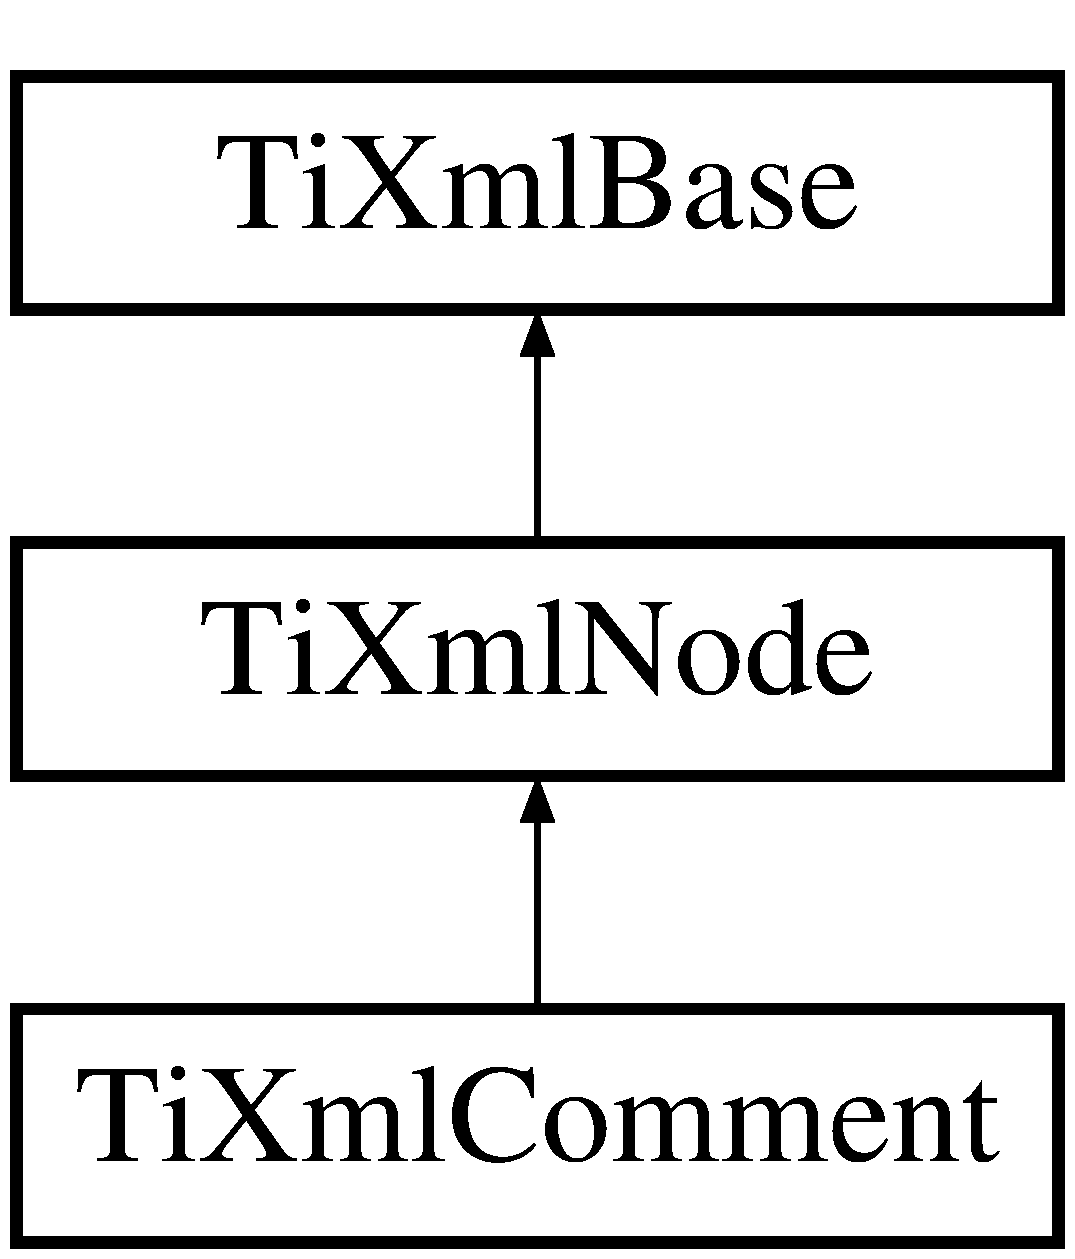
\includegraphics[height=3cm]{classTiXmlComment}
\end{center}
\end{figure}


\subsection{Detailed Description}
An XML comment. \subsection*{Public Member Functions}
\begin{CompactItemize}
\item 
{\bf TiXmlComment} ()
\begin{CompactList}\small\item\em Constructs an empty comment. \item\end{CompactList}\item 
{\bf TiXmlComment} (const char $\ast$\_\-value)
\begin{CompactList}\small\item\em Construct a comment from text. \item\end{CompactList}\item 
{\bf TiXmlComment} (const {\bf TiXmlComment} \&)
\item 
void {\bf operator=} (const {\bf TiXmlComment} \&base)
\item 
virtual {\bf $\sim$TiXmlComment} ()
\item 
virtual {\bf TiXmlNode} $\ast$ {\bf Clone} () const 
\begin{CompactList}\small\item\em Returns a copy of this Comment. \item\end{CompactList}\item 
virtual void {\bf Print} (FILE $\ast$cfile, int depth) const 
\item 
virtual const char $\ast$ {\bf Parse} (const char $\ast$p, {\bf TiXmlParsingData} $\ast$data, {\bf TiXmlEncoding} encoding)
\item 
virtual const {\bf TiXmlComment} $\ast$ {\bf ToComment} () const 
\begin{CompactList}\small\item\em Cast to a more defined type. Will return null not of the requested type. \item\end{CompactList}\item 
virtual {\bf TiXmlComment} $\ast$ {\bf ToComment} ()
\begin{CompactList}\small\item\em Cast to a more defined type. Will return null not of the requested type. \item\end{CompactList}\item 
virtual bool {\bf Accept} ({\bf TiXmlVisitor} $\ast$visitor) const 
\end{CompactItemize}
\subsection*{Protected Member Functions}
\begin{CompactItemize}
\item 
void {\bf CopyTo} ({\bf TiXmlComment} $\ast$target) const 
\end{CompactItemize}


\subsection{Constructor \& Destructor Documentation}
\index{TiXmlComment@{TiXmlComment}!TiXmlComment@{TiXmlComment}}
\index{TiXmlComment@{TiXmlComment}!TiXmlComment@{TiXmlComment}}
\subsubsection{\setlength{\rightskip}{0pt plus 5cm}TiXmlComment::TiXmlComment ()\hspace{0.3cm}{\tt  [inline]}}\label{classTiXmlComment_aa3252031d3e8bd3a2bf51a1c61201b7}


Constructs an empty comment. 

\index{TiXmlComment@{TiXmlComment}!TiXmlComment@{TiXmlComment}}
\index{TiXmlComment@{TiXmlComment}!TiXmlComment@{TiXmlComment}}
\subsubsection{\setlength{\rightskip}{0pt plus 5cm}TiXmlComment::TiXmlComment (const char $\ast$ {\em \_\-value})\hspace{0.3cm}{\tt  [inline]}}\label{classTiXmlComment_37e7802ef17bc03ebe5ae79bf0713d47}


Construct a comment from text. 

\index{TiXmlComment@{TiXmlComment}!TiXmlComment@{TiXmlComment}}
\index{TiXmlComment@{TiXmlComment}!TiXmlComment@{TiXmlComment}}
\subsubsection{\setlength{\rightskip}{0pt plus 5cm}TiXmlComment::TiXmlComment (const {\bf TiXmlComment} \& {\em copy})}\label{classTiXmlComment_faec41ac2760ce946ba1590eb5708e50}


\index{TiXmlComment@{TiXmlComment}!$\sim$TiXmlComment@{$\sim$TiXmlComment}}
\index{$\sim$TiXmlComment@{$\sim$TiXmlComment}!TiXmlComment@{TiXmlComment}}
\subsubsection{\setlength{\rightskip}{0pt plus 5cm}virtual TiXmlComment::$\sim$TiXmlComment ()\hspace{0.3cm}{\tt  [inline, virtual]}}\label{classTiXmlComment_3264ae2e9c4a127edfa03289bb2c9aa2}




\subsection{Member Function Documentation}
\index{TiXmlComment@{TiXmlComment}!operator=@{operator=}}
\index{operator=@{operator=}!TiXmlComment@{TiXmlComment}}
\subsubsection{\setlength{\rightskip}{0pt plus 5cm}void TiXmlComment::operator= (const {\bf TiXmlComment} \& {\em base})}\label{classTiXmlComment_46373f99b65cb960637dccb1f126bd49}


\index{TiXmlComment@{TiXmlComment}!Clone@{Clone}}
\index{Clone@{Clone}!TiXmlComment@{TiXmlComment}}
\subsubsection{\setlength{\rightskip}{0pt plus 5cm}{\bf TiXmlNode} $\ast$ TiXmlComment::Clone () const\hspace{0.3cm}{\tt  [virtual]}}\label{classTiXmlComment_4f6590c9c9a2b63a48972655b78eb853}


Returns a copy of this Comment. 



Implements {\bf TiXmlNode} \doxyref{}{p.}{classTiXmlNode_4508cc3a2d7a98e96a54cc09c37a78a4}.\index{TiXmlComment@{TiXmlComment}!Print@{Print}}
\index{Print@{Print}!TiXmlComment@{TiXmlComment}}
\subsubsection{\setlength{\rightskip}{0pt plus 5cm}void TiXmlComment::Print (FILE $\ast$ {\em cfile}, int {\em depth}) const\hspace{0.3cm}{\tt  [virtual]}}\label{classTiXmlComment_17398061d62c470f57801ce28fa33ad4}


All TinyXml classes can print themselves to a filestream or the string class (\doxyref{TiXmlString}{p.}{classTiXmlString} in non-STL mode, std::string in STL mode.) Either or both cfile and str can be null.

This is a formatted print, and will insert tabs and newlines.

(For an unformatted stream, use the $<$$<$ operator.) 

Implements {\bf TiXmlBase} \doxyref{}{p.}{classTiXmlBase_0de56b3f2ef14c65091a3b916437b512}.\index{TiXmlComment@{TiXmlComment}!Parse@{Parse}}
\index{Parse@{Parse}!TiXmlComment@{TiXmlComment}}
\subsubsection{\setlength{\rightskip}{0pt plus 5cm}const char $\ast$ TiXmlComment::Parse (const char $\ast$ {\em p}, {\bf TiXmlParsingData} $\ast$ {\em data}, {\bf TiXmlEncoding} {\em encoding})\hspace{0.3cm}{\tt  [virtual]}}\label{classTiXmlComment_43bddc18ac057734b41d84653b71d3e0}




Implements {\bf TiXmlBase} \doxyref{}{p.}{classTiXmlBase_00e4edb0219d00a1379c856e5a1d2025}.\index{TiXmlComment@{TiXmlComment}!ToComment@{ToComment}}
\index{ToComment@{ToComment}!TiXmlComment@{TiXmlComment}}
\subsubsection{\setlength{\rightskip}{0pt plus 5cm}virtual const {\bf TiXmlComment}$\ast$ TiXmlComment::ToComment () const\hspace{0.3cm}{\tt  [inline, virtual]}}\label{classTiXmlComment_00fb4215c20a2399ea05ac9b9e7e68a0}


Cast to a more defined type. Will return null not of the requested type. 



Reimplemented from {\bf TiXmlNode} \doxyref{}{p.}{classTiXmlNode_a0a5086f9eaee910bbfdc7f975e26574}.\index{TiXmlComment@{TiXmlComment}!ToComment@{ToComment}}
\index{ToComment@{ToComment}!TiXmlComment@{TiXmlComment}}
\subsubsection{\setlength{\rightskip}{0pt plus 5cm}virtual {\bf TiXmlComment}$\ast$ TiXmlComment::ToComment ()\hspace{0.3cm}{\tt  [inline, virtual]}}\label{classTiXmlComment_cc7c7e07e13c23f17797d642981511df}


Cast to a more defined type. Will return null not of the requested type. 



Reimplemented from {\bf TiXmlNode} \doxyref{}{p.}{classTiXmlNode_383e06a0787f7063953934867990f849}.\index{TiXmlComment@{TiXmlComment}!Accept@{Accept}}
\index{Accept@{Accept}!TiXmlComment@{TiXmlComment}}
\subsubsection{\setlength{\rightskip}{0pt plus 5cm}bool TiXmlComment::Accept ({\bf TiXmlVisitor} $\ast$ {\em visitor}) const\hspace{0.3cm}{\tt  [virtual]}}\label{classTiXmlComment_4382de0e50da973f11a23ea5852568bd}


Walk the XML tree visiting this node and all of its children. 

Implements {\bf TiXmlNode} \doxyref{}{p.}{classTiXmlNode_cc0f88b7462c6cb73809d410a4f5bb86}.\index{TiXmlComment@{TiXmlComment}!CopyTo@{CopyTo}}
\index{CopyTo@{CopyTo}!TiXmlComment@{TiXmlComment}}
\subsubsection{\setlength{\rightskip}{0pt plus 5cm}void TiXmlComment::CopyTo ({\bf TiXmlComment} $\ast$ {\em target}) const\hspace{0.3cm}{\tt  [protected]}}\label{classTiXmlComment_3175b2f27628f4fb7a043897930cd934}




The documentation for this class was generated from the following files:\begin{CompactItemize}
\item 
/home/msneddon/eclipse/galileoSR1\_\-cpp/workspace/NFsim/src/NFinput/TinyXML/{\bf tinyxml.h}\item 
/home/msneddon/eclipse/galileoSR1\_\-cpp/workspace/NFsim/src/NFinput/TinyXML/{\bf tinyxml.cpp}\item 
/home/msneddon/eclipse/galileoSR1\_\-cpp/workspace/NFsim/src/NFinput/TinyXML/{\bf tinyxmlparser.cpp}\end{CompactItemize}

\section{TiXmlCursor Struct Reference}
\label{structTiXmlCursor}\index{TiXmlCursor@{TiXmlCursor}}
{\tt \#include $<$tinyxml.h$>$}

\subsection*{Public Member Functions}
\begin{CompactItemize}
\item 
{\bf TiXmlCursor} ()
\item 
void {\bf Clear} ()
\end{CompactItemize}
\subsection*{Public Attributes}
\begin{CompactItemize}
\item 
int {\bf row}
\item 
int {\bf col}
\end{CompactItemize}


\subsection{Constructor \& Destructor Documentation}
\index{TiXmlCursor@{TiXmlCursor}!TiXmlCursor@{TiXmlCursor}}
\index{TiXmlCursor@{TiXmlCursor}!TiXmlCursor@{TiXmlCursor}}
\subsubsection{\setlength{\rightskip}{0pt plus 5cm}TiXmlCursor::TiXmlCursor ()\hspace{0.3cm}{\tt  [inline]}}\label{structTiXmlCursor_7ad233928a675f0271eb440b150e3ff1}




\subsection{Member Function Documentation}
\index{TiXmlCursor@{TiXmlCursor}!Clear@{Clear}}
\index{Clear@{Clear}!TiXmlCursor@{TiXmlCursor}}
\subsubsection{\setlength{\rightskip}{0pt plus 5cm}void TiXmlCursor::Clear ()\hspace{0.3cm}{\tt  [inline]}}\label{structTiXmlCursor_1e6fa622b59dafb71b6efe595105dcdd}




\subsection{Member Data Documentation}
\index{TiXmlCursor@{TiXmlCursor}!row@{row}}
\index{row@{row}!TiXmlCursor@{TiXmlCursor}}
\subsubsection{\setlength{\rightskip}{0pt plus 5cm}int {\bf TiXmlCursor::row}}\label{structTiXmlCursor_5b54dd949820c2db061e2be41f3effb3}


\index{TiXmlCursor@{TiXmlCursor}!col@{col}}
\index{col@{col}!TiXmlCursor@{TiXmlCursor}}
\subsubsection{\setlength{\rightskip}{0pt plus 5cm}int {\bf TiXmlCursor::col}}\label{structTiXmlCursor_5694d7ed2c4d20109d350c14c417969d}




The documentation for this struct was generated from the following file:\begin{CompactItemize}
\item 
/home/msneddon/eclipse/indigo/workspace/NFsim/src/NFinput/TinyXML/{\bf tinyxml.h}\end{CompactItemize}

\section{TiXmlDeclaration Class Reference}
\label{classTiXmlDeclaration}\index{TiXmlDeclaration@{TiXmlDeclaration}}
{\tt \#include $<$tinyxml.h$>$}

Inheritance diagram for TiXmlDeclaration::\begin{figure}[H]
\begin{center}
\leavevmode
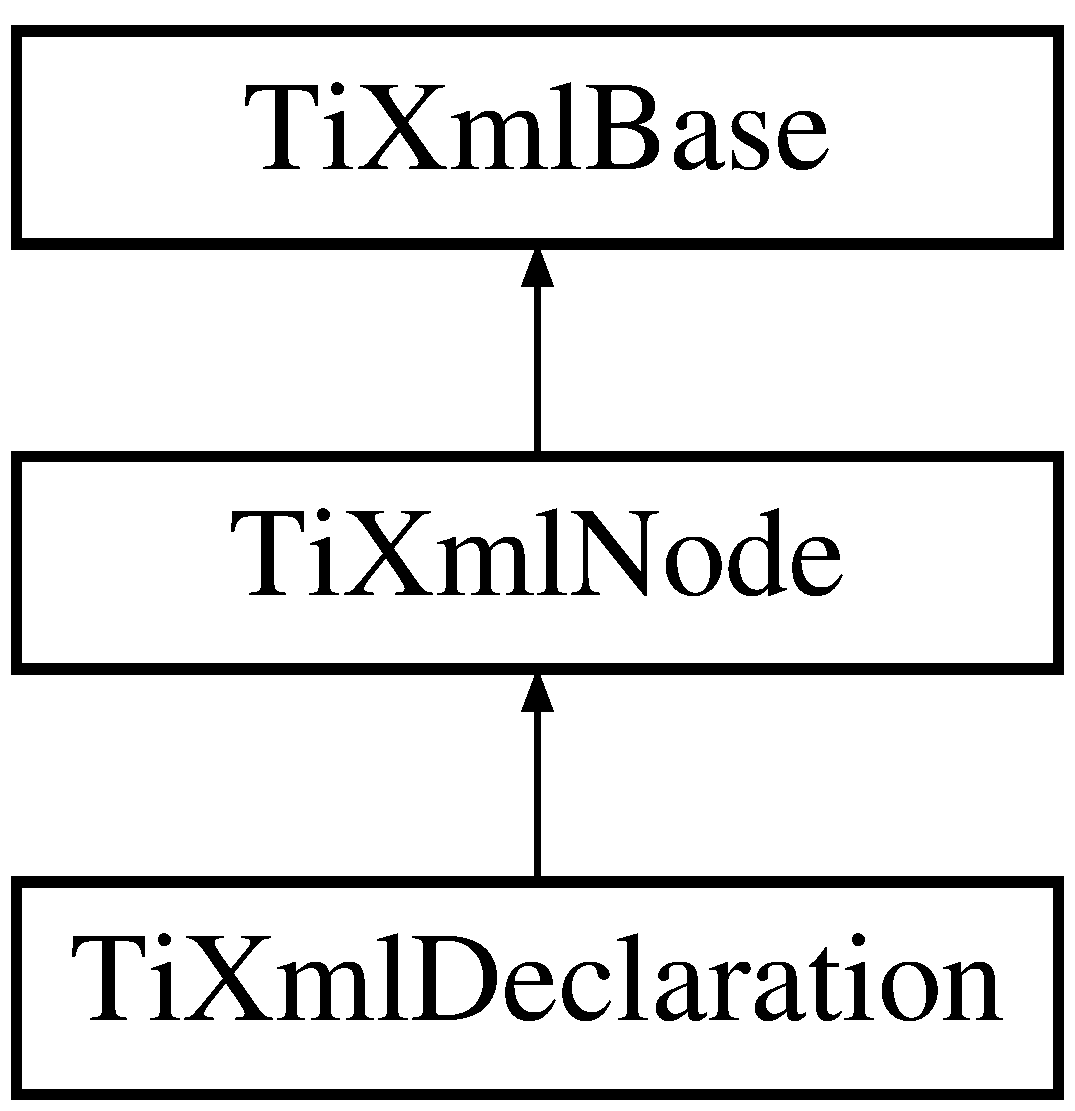
\includegraphics[height=3cm]{classTiXmlDeclaration}
\end{center}
\end{figure}


\subsection{Detailed Description}
In correct XML the declaration is the first entry in the file. 

\footnotesize\begin{verbatim}
		<?xml version="1.0" standalone="yes"?>
	\end{verbatim}
\normalsize


TinyXml will happily read or write files without a declaration, however. There are 3 possible attributes to the declaration: version, encoding, and standalone.

Note: In this version of the code, the attributes are handled as special cases, not generic attributes, simply because there can only be at most 3 and they are always the same. \subsection*{Public Member Functions}
\begin{CompactItemize}
\item 
{\bf TiXmlDeclaration} ()
\begin{CompactList}\small\item\em Construct an empty declaration. \item\end{CompactList}\item 
{\bf TiXmlDeclaration} (const char $\ast$\_\-version, const char $\ast$\_\-encoding, const char $\ast$\_\-standalone)
\begin{CompactList}\small\item\em Construct. \item\end{CompactList}\item 
{\bf TiXmlDeclaration} (const {\bf TiXmlDeclaration} \&copy)
\item 
void {\bf operator=} (const {\bf TiXmlDeclaration} \&copy)
\item 
virtual {\bf $\sim$TiXmlDeclaration} ()
\item 
const char $\ast$ {\bf Version} () const 
\begin{CompactList}\small\item\em Version. Will return an empty string if none was found. \item\end{CompactList}\item 
const char $\ast$ {\bf Encoding} () const 
\begin{CompactList}\small\item\em Encoding. Will return an empty string if none was found. \item\end{CompactList}\item 
const char $\ast$ {\bf Standalone} () const 
\begin{CompactList}\small\item\em Is this a standalone document? \item\end{CompactList}\item 
virtual {\bf TiXmlNode} $\ast$ {\bf Clone} () const 
\begin{CompactList}\small\item\em Creates a copy of this Declaration and returns it. \item\end{CompactList}\item 
virtual void {\bf Print} (FILE $\ast$cfile, int depth, TIXML\_\-STRING $\ast$str) const 
\item 
virtual void {\bf Print} (FILE $\ast$cfile, int depth) const 
\item 
virtual const char $\ast$ {\bf Parse} (const char $\ast$p, {\bf TiXmlParsingData} $\ast$data, {\bf TiXmlEncoding} encoding)
\item 
virtual const {\bf TiXmlDeclaration} $\ast$ {\bf ToDeclaration} () const 
\begin{CompactList}\small\item\em Cast to a more defined type. Will return null not of the requested type. \item\end{CompactList}\item 
virtual {\bf TiXmlDeclaration} $\ast$ {\bf ToDeclaration} ()
\begin{CompactList}\small\item\em Cast to a more defined type. Will return null not of the requested type. \item\end{CompactList}\item 
virtual bool {\bf Accept} ({\bf TiXmlVisitor} $\ast$visitor) const 
\end{CompactItemize}
\subsection*{Protected Member Functions}
\begin{CompactItemize}
\item 
void {\bf CopyTo} ({\bf TiXmlDeclaration} $\ast$target) const 
\end{CompactItemize}


\subsection{Constructor \& Destructor Documentation}
\index{TiXmlDeclaration@{TiXmlDeclaration}!TiXmlDeclaration@{TiXmlDeclaration}}
\index{TiXmlDeclaration@{TiXmlDeclaration}!TiXmlDeclaration@{TiXmlDeclaration}}
\subsubsection{\setlength{\rightskip}{0pt plus 5cm}TiXmlDeclaration::TiXmlDeclaration ()\hspace{0.3cm}{\tt  [inline]}}\label{classTiXmlDeclaration_a0484d059bea0ea1acb47c9094382d79}


Construct an empty declaration. 

\index{TiXmlDeclaration@{TiXmlDeclaration}!TiXmlDeclaration@{TiXmlDeclaration}}
\index{TiXmlDeclaration@{TiXmlDeclaration}!TiXmlDeclaration@{TiXmlDeclaration}}
\subsubsection{\setlength{\rightskip}{0pt plus 5cm}TiXmlDeclaration::TiXmlDeclaration (const char $\ast$ {\em \_\-version}, const char $\ast$ {\em \_\-encoding}, const char $\ast$ {\em \_\-standalone})}\label{classTiXmlDeclaration_3b618d1c30c25e4b7a71f31a595ee298}


Construct. 

\index{TiXmlDeclaration@{TiXmlDeclaration}!TiXmlDeclaration@{TiXmlDeclaration}}
\index{TiXmlDeclaration@{TiXmlDeclaration}!TiXmlDeclaration@{TiXmlDeclaration}}
\subsubsection{\setlength{\rightskip}{0pt plus 5cm}TiXmlDeclaration::TiXmlDeclaration (const {\bf TiXmlDeclaration} \& {\em copy})}\label{classTiXmlDeclaration_58ac9042c342f7845c8491da0bb091e8}


\index{TiXmlDeclaration@{TiXmlDeclaration}!$\sim$TiXmlDeclaration@{$\sim$TiXmlDeclaration}}
\index{$\sim$TiXmlDeclaration@{$\sim$TiXmlDeclaration}!TiXmlDeclaration@{TiXmlDeclaration}}
\subsubsection{\setlength{\rightskip}{0pt plus 5cm}virtual TiXmlDeclaration::$\sim$TiXmlDeclaration ()\hspace{0.3cm}{\tt  [inline, virtual]}}\label{classTiXmlDeclaration_d5f37a673f4c507fd7e550470f9cec25}




\subsection{Member Function Documentation}
\index{TiXmlDeclaration@{TiXmlDeclaration}!operator=@{operator=}}
\index{operator=@{operator=}!TiXmlDeclaration@{TiXmlDeclaration}}
\subsubsection{\setlength{\rightskip}{0pt plus 5cm}void TiXmlDeclaration::operator= (const {\bf TiXmlDeclaration} \& {\em copy})}\label{classTiXmlDeclaration_0fedc57539af9049be8db2d7d9d9ba33}


\index{TiXmlDeclaration@{TiXmlDeclaration}!Version@{Version}}
\index{Version@{Version}!TiXmlDeclaration@{TiXmlDeclaration}}
\subsubsection{\setlength{\rightskip}{0pt plus 5cm}const char$\ast$ TiXmlDeclaration::Version () const\hspace{0.3cm}{\tt  [inline]}}\label{classTiXmlDeclaration_02ee557b1a4545c3219ed377c103ec76}


Version. Will return an empty string if none was found. 

\index{TiXmlDeclaration@{TiXmlDeclaration}!Encoding@{Encoding}}
\index{Encoding@{Encoding}!TiXmlDeclaration@{TiXmlDeclaration}}
\subsubsection{\setlength{\rightskip}{0pt plus 5cm}const char$\ast$ TiXmlDeclaration::Encoding () const\hspace{0.3cm}{\tt  [inline]}}\label{classTiXmlDeclaration_5d974231f9e9a2f0542f15f3a46cdb76}


Encoding. Will return an empty string if none was found. 

\index{TiXmlDeclaration@{TiXmlDeclaration}!Standalone@{Standalone}}
\index{Standalone@{Standalone}!TiXmlDeclaration@{TiXmlDeclaration}}
\subsubsection{\setlength{\rightskip}{0pt plus 5cm}const char$\ast$ TiXmlDeclaration::Standalone () const\hspace{0.3cm}{\tt  [inline]}}\label{classTiXmlDeclaration_9ff06afc033d7ef730ec7c6825b97ad9}


Is this a standalone document? 

\index{TiXmlDeclaration@{TiXmlDeclaration}!Clone@{Clone}}
\index{Clone@{Clone}!TiXmlDeclaration@{TiXmlDeclaration}}
\subsubsection{\setlength{\rightskip}{0pt plus 5cm}{\bf TiXmlNode} $\ast$ TiXmlDeclaration::Clone () const\hspace{0.3cm}{\tt  [virtual]}}\label{classTiXmlDeclaration_ff8231266d735943d8a7514a9c9822b9}


Creates a copy of this Declaration and returns it. 



Implements {\bf TiXmlNode} \doxyref{}{p.}{classTiXmlNode_4508cc3a2d7a98e96a54cc09c37a78a4}.\index{TiXmlDeclaration@{TiXmlDeclaration}!Print@{Print}}
\index{Print@{Print}!TiXmlDeclaration@{TiXmlDeclaration}}
\subsubsection{\setlength{\rightskip}{0pt plus 5cm}void TiXmlDeclaration::Print (FILE $\ast$ {\em cfile}, int {\em depth}, TIXML\_\-STRING $\ast$ {\em str}) const\hspace{0.3cm}{\tt  [virtual]}}\label{classTiXmlDeclaration_a5ab32ec19d4eeecff4a9238c6c90565}


\index{TiXmlDeclaration@{TiXmlDeclaration}!Print@{Print}}
\index{Print@{Print}!TiXmlDeclaration@{TiXmlDeclaration}}
\subsubsection{\setlength{\rightskip}{0pt plus 5cm}virtual void TiXmlDeclaration::Print (FILE $\ast$ {\em cfile}, int {\em depth}) const\hspace{0.3cm}{\tt  [inline, virtual]}}\label{classTiXmlDeclaration_bf6303db4bd05b5be554036817ff1cb4}


All TinyXml classes can print themselves to a filestream or the string class (\doxyref{TiXmlString}{p.}{classTiXmlString} in non-STL mode, std::string in STL mode.) Either or both cfile and str can be null.

This is a formatted print, and will insert tabs and newlines.

(For an unformatted stream, use the $<$$<$ operator.) 

Implements {\bf TiXmlBase} \doxyref{}{p.}{classTiXmlBase_0de56b3f2ef14c65091a3b916437b512}.\index{TiXmlDeclaration@{TiXmlDeclaration}!Parse@{Parse}}
\index{Parse@{Parse}!TiXmlDeclaration@{TiXmlDeclaration}}
\subsubsection{\setlength{\rightskip}{0pt plus 5cm}const char $\ast$ TiXmlDeclaration::Parse (const char $\ast$ {\em p}, {\bf TiXmlParsingData} $\ast$ {\em data}, {\bf TiXmlEncoding} {\em encoding})\hspace{0.3cm}{\tt  [virtual]}}\label{classTiXmlDeclaration_9839ea97ed687a2b7342fd7b0f04361b}




Implements {\bf TiXmlBase} \doxyref{}{p.}{classTiXmlBase_00e4edb0219d00a1379c856e5a1d2025}.\index{TiXmlDeclaration@{TiXmlDeclaration}!ToDeclaration@{ToDeclaration}}
\index{ToDeclaration@{ToDeclaration}!TiXmlDeclaration@{TiXmlDeclaration}}
\subsubsection{\setlength{\rightskip}{0pt plus 5cm}virtual const {\bf TiXmlDeclaration}$\ast$ TiXmlDeclaration::ToDeclaration () const\hspace{0.3cm}{\tt  [inline, virtual]}}\label{classTiXmlDeclaration_1e085d3fefd1dbf5ccdbff729931a967}


Cast to a more defined type. Will return null not of the requested type. 



Reimplemented from {\bf TiXmlNode} \doxyref{}{p.}{classTiXmlNode_9f43e6984fc7d4afd6eb32714c6b7b72}.\index{TiXmlDeclaration@{TiXmlDeclaration}!ToDeclaration@{ToDeclaration}}
\index{ToDeclaration@{ToDeclaration}!TiXmlDeclaration@{TiXmlDeclaration}}
\subsubsection{\setlength{\rightskip}{0pt plus 5cm}virtual {\bf TiXmlDeclaration}$\ast$ TiXmlDeclaration::ToDeclaration ()\hspace{0.3cm}{\tt  [inline, virtual]}}\label{classTiXmlDeclaration_6bd3d1daddcaeb9543c24bfd090969ce}


Cast to a more defined type. Will return null not of the requested type. 



Reimplemented from {\bf TiXmlNode} \doxyref{}{p.}{classTiXmlNode_4027136ca820ff4a636b607231b6a6df}.\index{TiXmlDeclaration@{TiXmlDeclaration}!Accept@{Accept}}
\index{Accept@{Accept}!TiXmlDeclaration@{TiXmlDeclaration}}
\subsubsection{\setlength{\rightskip}{0pt plus 5cm}bool TiXmlDeclaration::Accept ({\bf TiXmlVisitor} $\ast$ {\em visitor}) const\hspace{0.3cm}{\tt  [virtual]}}\label{classTiXmlDeclaration_b6a6b178161ba9abc2c35058de689864}


Walk the XML tree visiting this node and all of its children. 

Implements {\bf TiXmlNode} \doxyref{}{p.}{classTiXmlNode_cc0f88b7462c6cb73809d410a4f5bb86}.\index{TiXmlDeclaration@{TiXmlDeclaration}!CopyTo@{CopyTo}}
\index{CopyTo@{CopyTo}!TiXmlDeclaration@{TiXmlDeclaration}}
\subsubsection{\setlength{\rightskip}{0pt plus 5cm}void TiXmlDeclaration::CopyTo ({\bf TiXmlDeclaration} $\ast$ {\em target}) const\hspace{0.3cm}{\tt  [protected]}}\label{classTiXmlDeclaration_9d08959f935421a593032bd3efb30c38}




The documentation for this class was generated from the following files:\begin{CompactItemize}
\item 
/home/msneddon/eclipse/indigo/workspace/NFsim/src/NFinput/TinyXML/{\bf tinyxml.h}\item 
/home/msneddon/eclipse/indigo/workspace/NFsim/src/NFinput/TinyXML/{\bf tinyxml.cpp}\item 
/home/msneddon/eclipse/indigo/workspace/NFsim/src/NFinput/TinyXML/{\bf tinyxmlparser.cpp}\end{CompactItemize}

\section{TiXmlDocument Class Reference}
\label{classTiXmlDocument}\index{TiXmlDocument@{TiXmlDocument}}
{\tt \#include $<$tinyxml.h$>$}

Inheritance diagram for TiXmlDocument::\begin{figure}[H]
\begin{center}
\leavevmode
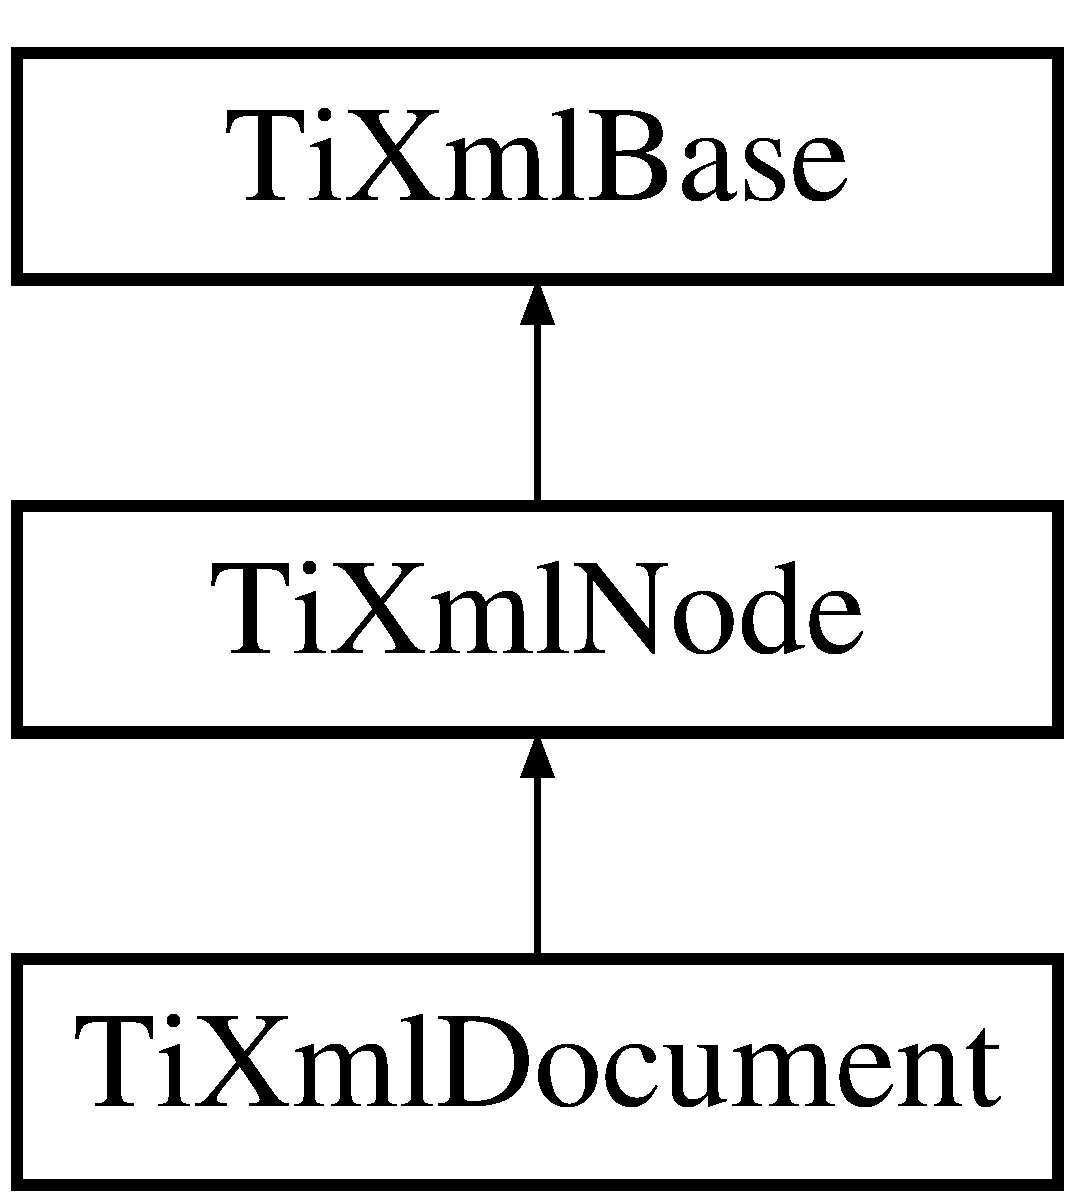
\includegraphics[height=3cm]{classTiXmlDocument}
\end{center}
\end{figure}


\subsection{Detailed Description}
Always the top level node. A document binds together all the XML pieces. It can be saved, loaded, and printed to the screen. The 'value' of a document node is the xml file name. \subsection*{Public Member Functions}
\begin{CompactItemize}
\item 
{\bf TiXmlDocument} ()
\begin{CompactList}\small\item\em Create an empty document, that has no name. \item\end{CompactList}\item 
{\bf TiXmlDocument} (const char $\ast$documentName)
\begin{CompactList}\small\item\em Create a document with a name. The name of the document is also the filename of the xml. \item\end{CompactList}\item 
{\bf TiXmlDocument} (const {\bf TiXmlDocument} \&copy)
\item 
void {\bf operator=} (const {\bf TiXmlDocument} \&copy)
\item 
virtual {\bf $\sim$TiXmlDocument} ()
\item 
bool {\bf LoadFile} ({\bf TiXmlEncoding} encoding={\bf TIXML\_\-DEFAULT\_\-ENCODING})
\item 
bool {\bf SaveFile} () const 
\begin{CompactList}\small\item\em Save a file using the current document value. Returns true if successful. \item\end{CompactList}\item 
bool {\bf LoadFile} (const char $\ast$filename, {\bf TiXmlEncoding} encoding={\bf TIXML\_\-DEFAULT\_\-ENCODING})
\begin{CompactList}\small\item\em Load a file using the given filename. Returns true if successful. \item\end{CompactList}\item 
bool {\bf SaveFile} (const char $\ast$filename) const 
\begin{CompactList}\small\item\em Save a file using the given filename. Returns true if successful. \item\end{CompactList}\item 
bool {\bf LoadFile} (FILE $\ast$, {\bf TiXmlEncoding} encoding={\bf TIXML\_\-DEFAULT\_\-ENCODING})
\item 
bool {\bf SaveFile} (FILE $\ast$) const 
\begin{CompactList}\small\item\em Save a file using the given FILE$\ast$. Returns true if successful. \item\end{CompactList}\item 
virtual const char $\ast$ {\bf Parse} (const char $\ast$p, {\bf TiXmlParsingData} $\ast$data=0, {\bf TiXmlEncoding} encoding={\bf TIXML\_\-DEFAULT\_\-ENCODING})
\item 
const {\bf TiXmlElement} $\ast$ {\bf RootElement} () const 
\item 
{\bf TiXmlElement} $\ast$ {\bf RootElement} ()
\item 
bool {\bf Error} () const 
\item 
const char $\ast$ {\bf ErrorDesc} () const 
\begin{CompactList}\small\item\em Contains a textual (english) description of the error if one occurs. \item\end{CompactList}\item 
int {\bf ErrorId} () const 
\item 
int {\bf ErrorRow} () const 
\item 
int {\bf ErrorCol} () const 
\begin{CompactList}\small\item\em The column where the error occured. See \doxyref{ErrorRow()}{p.}{classTiXmlDocument_f30efc75e804aa2e92fb8be3a8cb676e}. \item\end{CompactList}\item 
void {\bf SetTabSize} (int \_\-tabsize)
\item 
int {\bf TabSize} () const 
\item 
void {\bf ClearError} ()
\item 
void {\bf Print} () const 
\item 
virtual void {\bf Print} (FILE $\ast$cfile, int depth=0) const 
\begin{CompactList}\small\item\em Print this Document to a FILE stream. \item\end{CompactList}\item 
void {\bf SetError} (int err, const char $\ast$errorLocation, {\bf TiXmlParsingData} $\ast$prevData, {\bf TiXmlEncoding} encoding)
\item 
virtual const {\bf TiXmlDocument} $\ast$ {\bf ToDocument} () const 
\begin{CompactList}\small\item\em Cast to a more defined type. Will return null not of the requested type. \item\end{CompactList}\item 
virtual {\bf TiXmlDocument} $\ast$ {\bf ToDocument} ()
\begin{CompactList}\small\item\em Cast to a more defined type. Will return null not of the requested type. \item\end{CompactList}\item 
virtual bool {\bf Accept} ({\bf TiXmlVisitor} $\ast$content) const 
\end{CompactItemize}
\subsection*{Protected Member Functions}
\begin{CompactItemize}
\item 
virtual {\bf TiXmlNode} $\ast$ {\bf Clone} () const 
\end{CompactItemize}


\subsection{Constructor \& Destructor Documentation}
\index{TiXmlDocument@{TiXmlDocument}!TiXmlDocument@{TiXmlDocument}}
\index{TiXmlDocument@{TiXmlDocument}!TiXmlDocument@{TiXmlDocument}}
\subsubsection{\setlength{\rightskip}{0pt plus 5cm}TiXmlDocument::TiXmlDocument ()}\label{classTiXmlDocument_9f5e84335708fde98400230f9f12659c}


Create an empty document, that has no name. 

\index{TiXmlDocument@{TiXmlDocument}!TiXmlDocument@{TiXmlDocument}}
\index{TiXmlDocument@{TiXmlDocument}!TiXmlDocument@{TiXmlDocument}}
\subsubsection{\setlength{\rightskip}{0pt plus 5cm}TiXmlDocument::TiXmlDocument (const char $\ast$ {\em documentName})}\label{classTiXmlDocument_e4508b452d0c3061db085f3db27b8396}


Create a document with a name. The name of the document is also the filename of the xml. 

\index{TiXmlDocument@{TiXmlDocument}!TiXmlDocument@{TiXmlDocument}}
\index{TiXmlDocument@{TiXmlDocument}!TiXmlDocument@{TiXmlDocument}}
\subsubsection{\setlength{\rightskip}{0pt plus 5cm}TiXmlDocument::TiXmlDocument (const {\bf TiXmlDocument} \& {\em copy})}\label{classTiXmlDocument_323a7486e7da6099cdc19a5ff7e74b07}


\index{TiXmlDocument@{TiXmlDocument}!$\sim$TiXmlDocument@{$\sim$TiXmlDocument}}
\index{$\sim$TiXmlDocument@{$\sim$TiXmlDocument}!TiXmlDocument@{TiXmlDocument}}
\subsubsection{\setlength{\rightskip}{0pt plus 5cm}virtual TiXmlDocument::$\sim$TiXmlDocument ()\hspace{0.3cm}{\tt  [inline, virtual]}}\label{classTiXmlDocument_1b8a035c2c2aab38e4387246a0b712c5}




\subsection{Member Function Documentation}
\index{TiXmlDocument@{TiXmlDocument}!operator=@{operator=}}
\index{operator=@{operator=}!TiXmlDocument@{TiXmlDocument}}
\subsubsection{\setlength{\rightskip}{0pt plus 5cm}void TiXmlDocument::operator= (const {\bf TiXmlDocument} \& {\em copy})}\label{classTiXmlDocument_afbfacc3414008f619b1345775ef12a4}


\index{TiXmlDocument@{TiXmlDocument}!LoadFile@{LoadFile}}
\index{LoadFile@{LoadFile}!TiXmlDocument@{TiXmlDocument}}
\subsubsection{\setlength{\rightskip}{0pt plus 5cm}bool TiXmlDocument::LoadFile ({\bf TiXmlEncoding} {\em encoding} = {\tt {\bf TIXML\_\-DEFAULT\_\-ENCODING}})}\label{classTiXmlDocument_4c852a889c02cf251117fd1d9fe1845f}


Load a file using the current document value. Returns true if successful. Will delete any existing document data before loading. \index{TiXmlDocument@{TiXmlDocument}!SaveFile@{SaveFile}}
\index{SaveFile@{SaveFile}!TiXmlDocument@{TiXmlDocument}}
\subsubsection{\setlength{\rightskip}{0pt plus 5cm}bool TiXmlDocument::SaveFile () const}\label{classTiXmlDocument_21c0aeb0d0a720169ad4ac89523ebe93}


Save a file using the current document value. Returns true if successful. 

\index{TiXmlDocument@{TiXmlDocument}!LoadFile@{LoadFile}}
\index{LoadFile@{LoadFile}!TiXmlDocument@{TiXmlDocument}}
\subsubsection{\setlength{\rightskip}{0pt plus 5cm}bool TiXmlDocument::LoadFile (const char $\ast$ {\em filename}, {\bf TiXmlEncoding} {\em encoding} = {\tt {\bf TIXML\_\-DEFAULT\_\-ENCODING}})}\label{classTiXmlDocument_879cdf5e981b8b2d2ef82f2546dd28fb}


Load a file using the given filename. Returns true if successful. 

\index{TiXmlDocument@{TiXmlDocument}!SaveFile@{SaveFile}}
\index{SaveFile@{SaveFile}!TiXmlDocument@{TiXmlDocument}}
\subsubsection{\setlength{\rightskip}{0pt plus 5cm}bool TiXmlDocument::SaveFile (const char $\ast$ {\em filename}) const}\label{classTiXmlDocument_e869f5ebf7fc54c4a1d737fb4689fd44}


Save a file using the given filename. Returns true if successful. 

\index{TiXmlDocument@{TiXmlDocument}!LoadFile@{LoadFile}}
\index{LoadFile@{LoadFile}!TiXmlDocument@{TiXmlDocument}}
\subsubsection{\setlength{\rightskip}{0pt plus 5cm}bool TiXmlDocument::LoadFile (FILE $\ast$ {\em file}, {\bf TiXmlEncoding} {\em encoding} = {\tt {\bf TIXML\_\-DEFAULT\_\-ENCODING}})}\label{classTiXmlDocument_41f6fe7200864d1dca663d230caf8db6}


Load a file using the given FILE$\ast$. Returns true if successful. Note that this method doesn't stream - the entire object pointed at by the FILE$\ast$ will be interpreted as an XML file. TinyXML doesn't stream in XML from the current file location. Streaming may be added in the future. \index{TiXmlDocument@{TiXmlDocument}!SaveFile@{SaveFile}}
\index{SaveFile@{SaveFile}!TiXmlDocument@{TiXmlDocument}}
\subsubsection{\setlength{\rightskip}{0pt plus 5cm}bool TiXmlDocument::SaveFile (FILE $\ast$ {\em fp}) const}\label{classTiXmlDocument_cf1672b4538c6d1d441f9f108aea2bf4}


Save a file using the given FILE$\ast$. Returns true if successful. 

\index{TiXmlDocument@{TiXmlDocument}!Parse@{Parse}}
\index{Parse@{Parse}!TiXmlDocument@{TiXmlDocument}}
\subsubsection{\setlength{\rightskip}{0pt plus 5cm}const char $\ast$ TiXmlDocument::Parse (const char $\ast$ {\em p}, {\bf TiXmlParsingData} $\ast$ {\em data} = {\tt 0}, {\bf TiXmlEncoding} {\em encoding} = {\tt {\bf TIXML\_\-DEFAULT\_\-ENCODING}})\hspace{0.3cm}{\tt  [virtual]}}\label{classTiXmlDocument_789ad2f06f93d52bdb5570b2f3670289}


Parse the given null terminated block of xml data. Passing in an encoding to this method (either TIXML\_\-ENCODING\_\-LEGACY or TIXML\_\-ENCODING\_\-UTF8 will force TinyXml to use that encoding, regardless of what TinyXml might otherwise try to detect. 

Implements {\bf TiXmlBase} \doxyref{}{p.}{classTiXmlBase_00e4edb0219d00a1379c856e5a1d2025}.\index{TiXmlDocument@{TiXmlDocument}!RootElement@{RootElement}}
\index{RootElement@{RootElement}!TiXmlDocument@{TiXmlDocument}}
\subsubsection{\setlength{\rightskip}{0pt plus 5cm}const {\bf TiXmlElement}$\ast$ TiXmlDocument::RootElement () const\hspace{0.3cm}{\tt  [inline]}}\label{classTiXmlDocument_d09d17927f908f40efb406af2fb873be}


Get the root element -- the only top level element -- of the document. In well formed XML, there should only be one. TinyXml is tolerant of multiple elements at the document level. \index{TiXmlDocument@{TiXmlDocument}!RootElement@{RootElement}}
\index{RootElement@{RootElement}!TiXmlDocument@{TiXmlDocument}}
\subsubsection{\setlength{\rightskip}{0pt plus 5cm}{\bf TiXmlElement}$\ast$ TiXmlDocument::RootElement ()\hspace{0.3cm}{\tt  [inline]}}\label{classTiXmlDocument_0b43e762a23f938b06651bc90b8a1013}


\index{TiXmlDocument@{TiXmlDocument}!Error@{Error}}
\index{Error@{Error}!TiXmlDocument@{TiXmlDocument}}
\subsubsection{\setlength{\rightskip}{0pt plus 5cm}bool TiXmlDocument::Error () const\hspace{0.3cm}{\tt  [inline]}}\label{classTiXmlDocument_6dfc01a6e5d58e56acd537dfd3bdeb29}


If an error occurs, Error will be set to true. Also,\begin{itemize}
\item The \doxyref{ErrorId()}{p.}{classTiXmlDocument_f96fc2f3f9ec6422782bfe916c9e778f} will contain the integer identifier of the error (not generally useful)\item The \doxyref{ErrorDesc()}{p.}{classTiXmlDocument_9d0f689f6e09ea494ea547be8d79c25e} method will return the name of the error. (very useful)\item The \doxyref{ErrorRow()}{p.}{classTiXmlDocument_f30efc75e804aa2e92fb8be3a8cb676e} and \doxyref{ErrorCol()}{p.}{classTiXmlDocument_a90bc630ee5203c6109ca5fad3323649} will return the location of the error (if known) \end{itemize}
\index{TiXmlDocument@{TiXmlDocument}!ErrorDesc@{ErrorDesc}}
\index{ErrorDesc@{ErrorDesc}!TiXmlDocument@{TiXmlDocument}}
\subsubsection{\setlength{\rightskip}{0pt plus 5cm}const char$\ast$ TiXmlDocument::ErrorDesc () const\hspace{0.3cm}{\tt  [inline]}}\label{classTiXmlDocument_9d0f689f6e09ea494ea547be8d79c25e}


Contains a textual (english) description of the error if one occurs. 

\index{TiXmlDocument@{TiXmlDocument}!ErrorId@{ErrorId}}
\index{ErrorId@{ErrorId}!TiXmlDocument@{TiXmlDocument}}
\subsubsection{\setlength{\rightskip}{0pt plus 5cm}int TiXmlDocument::ErrorId () const\hspace{0.3cm}{\tt  [inline]}}\label{classTiXmlDocument_f96fc2f3f9ec6422782bfe916c9e778f}


Generally, you probably want the error string ( \doxyref{ErrorDesc()}{p.}{classTiXmlDocument_9d0f689f6e09ea494ea547be8d79c25e} ). But if you prefer the ErrorId, this function will fetch it. \index{TiXmlDocument@{TiXmlDocument}!ErrorRow@{ErrorRow}}
\index{ErrorRow@{ErrorRow}!TiXmlDocument@{TiXmlDocument}}
\subsubsection{\setlength{\rightskip}{0pt plus 5cm}int TiXmlDocument::ErrorRow () const\hspace{0.3cm}{\tt  [inline]}}\label{classTiXmlDocument_f30efc75e804aa2e92fb8be3a8cb676e}


Returns the location (if known) of the error. The first column is column 1, and the first row is row 1. A value of 0 means the row and column wasn't applicable (memory errors, for example, have no row/column) or the parser lost the error. (An error in the error reporting, in that case.)

\begin{Desc}
\item[See also:]\doxyref{SetTabSize}{p.}{classTiXmlDocument_51dac56316f89b35bdb7d0d433ba988e}, \doxyref{Row}{p.}{classTiXmlBase_024bceb070188df92c2a8d8852dd0853}, \doxyref{Column}{p.}{classTiXmlBase_b54bfb9b70fe6dd276e7b279cab7f003} \end{Desc}
\index{TiXmlDocument@{TiXmlDocument}!ErrorCol@{ErrorCol}}
\index{ErrorCol@{ErrorCol}!TiXmlDocument@{TiXmlDocument}}
\subsubsection{\setlength{\rightskip}{0pt plus 5cm}int TiXmlDocument::ErrorCol () const\hspace{0.3cm}{\tt  [inline]}}\label{classTiXmlDocument_a90bc630ee5203c6109ca5fad3323649}


The column where the error occured. See \doxyref{ErrorRow()}{p.}{classTiXmlDocument_f30efc75e804aa2e92fb8be3a8cb676e}. 

\index{TiXmlDocument@{TiXmlDocument}!SetTabSize@{SetTabSize}}
\index{SetTabSize@{SetTabSize}!TiXmlDocument@{TiXmlDocument}}
\subsubsection{\setlength{\rightskip}{0pt plus 5cm}void TiXmlDocument::SetTabSize (int {\em \_\-tabsize})\hspace{0.3cm}{\tt  [inline]}}\label{classTiXmlDocument_51dac56316f89b35bdb7d0d433ba988e}


\doxyref{SetTabSize()}{p.}{classTiXmlDocument_51dac56316f89b35bdb7d0d433ba988e} allows the error reporting functions (\doxyref{ErrorRow()}{p.}{classTiXmlDocument_f30efc75e804aa2e92fb8be3a8cb676e} and \doxyref{ErrorCol()}{p.}{classTiXmlDocument_a90bc630ee5203c6109ca5fad3323649}) to report the correct values for row and column. It does not change the output or input in any way.

By calling this method, with a tab size greater than 0, the row and column of each node and attribute is stored when the file is loaded. Very useful for tracking the DOM back in to the source file.

The tab size is required for calculating the location of nodes. If not set, the default of 4 is used. The tabsize is set per document. Setting the tabsize to 0 disables row/column tracking.

Note that row and column tracking is not supported when using operator$>$$>$.

The tab size needs to be enabled before the parse or load. Correct usage: 

\footnotesize\begin{verbatim}
		TiXmlDocument doc;
		doc.SetTabSize( 8 );
		doc.Load( "myfile.xml" );
		\end{verbatim}
\normalsize


\begin{Desc}
\item[See also:]\doxyref{Row}{p.}{classTiXmlBase_024bceb070188df92c2a8d8852dd0853}, \doxyref{Column}{p.}{classTiXmlBase_b54bfb9b70fe6dd276e7b279cab7f003} \end{Desc}
\index{TiXmlDocument@{TiXmlDocument}!TabSize@{TabSize}}
\index{TabSize@{TabSize}!TiXmlDocument@{TiXmlDocument}}
\subsubsection{\setlength{\rightskip}{0pt plus 5cm}int TiXmlDocument::TabSize () const\hspace{0.3cm}{\tt  [inline]}}\label{classTiXmlDocument_612360241b85bad0826b2a9ae9cda561}


\index{TiXmlDocument@{TiXmlDocument}!ClearError@{ClearError}}
\index{ClearError@{ClearError}!TiXmlDocument@{TiXmlDocument}}
\subsubsection{\setlength{\rightskip}{0pt plus 5cm}void TiXmlDocument::ClearError ()\hspace{0.3cm}{\tt  [inline]}}\label{classTiXmlDocument_c66b8c28db86363315712a3574e87c35}


If you have handled the error, it can be reset with this call. The error state is automatically cleared if you Parse a new XML block. \index{TiXmlDocument@{TiXmlDocument}!Print@{Print}}
\index{Print@{Print}!TiXmlDocument@{TiXmlDocument}}
\subsubsection{\setlength{\rightskip}{0pt plus 5cm}void TiXmlDocument::Print () const\hspace{0.3cm}{\tt  [inline]}}\label{classTiXmlDocument_f08389ec70ee9b2de7f800e206a18510}


Write the document to standard out using formatted printing (\char`\"{}pretty print\char`\"{}). \index{TiXmlDocument@{TiXmlDocument}!Print@{Print}}
\index{Print@{Print}!TiXmlDocument@{TiXmlDocument}}
\subsubsection{\setlength{\rightskip}{0pt plus 5cm}void TiXmlDocument::Print (FILE $\ast$ {\em cfile}, int {\em depth} = {\tt 0}) const\hspace{0.3cm}{\tt  [virtual]}}\label{classTiXmlDocument_7b1aea204fee266b70b9c105c8bf2ada}


Print this Document to a FILE stream. 



Implements {\bf TiXmlBase} \doxyref{}{p.}{classTiXmlBase_0de56b3f2ef14c65091a3b916437b512}.\index{TiXmlDocument@{TiXmlDocument}!SetError@{SetError}}
\index{SetError@{SetError}!TiXmlDocument@{TiXmlDocument}}
\subsubsection{\setlength{\rightskip}{0pt plus 5cm}void TiXmlDocument::SetError (int {\em err}, const char $\ast$ {\em errorLocation}, {\bf TiXmlParsingData} $\ast$ {\em prevData}, {\bf TiXmlEncoding} {\em encoding})}\label{classTiXmlDocument_735c23e318597b920c94eae77fa206de}


\index{TiXmlDocument@{TiXmlDocument}!ToDocument@{ToDocument}}
\index{ToDocument@{ToDocument}!TiXmlDocument@{TiXmlDocument}}
\subsubsection{\setlength{\rightskip}{0pt plus 5cm}virtual const {\bf TiXmlDocument}$\ast$ TiXmlDocument::ToDocument () const\hspace{0.3cm}{\tt  [inline, virtual]}}\label{classTiXmlDocument_1dc977bde3e4fe85a8eb9d88a35ef5a4}


Cast to a more defined type. Will return null not of the requested type. 



Reimplemented from {\bf TiXmlNode} \doxyref{}{p.}{classTiXmlNode_8a4cda4b15c29f64cff419309aebed08}.\index{TiXmlDocument@{TiXmlDocument}!ToDocument@{ToDocument}}
\index{ToDocument@{ToDocument}!TiXmlDocument@{TiXmlDocument}}
\subsubsection{\setlength{\rightskip}{0pt plus 5cm}virtual {\bf TiXmlDocument}$\ast$ TiXmlDocument::ToDocument ()\hspace{0.3cm}{\tt  [inline, virtual]}}\label{classTiXmlDocument_1025d942a1f328fd742d545e37efdd42}


Cast to a more defined type. Will return null not of the requested type. 



Reimplemented from {\bf TiXmlNode} \doxyref{}{p.}{classTiXmlNode_6a4c8ac28ee7a745d059db6691e03bae}.\index{TiXmlDocument@{TiXmlDocument}!Accept@{Accept}}
\index{Accept@{Accept}!TiXmlDocument@{TiXmlDocument}}
\subsubsection{\setlength{\rightskip}{0pt plus 5cm}bool TiXmlDocument::Accept ({\bf TiXmlVisitor} $\ast$ {\em content}) const\hspace{0.3cm}{\tt  [virtual]}}\label{classTiXmlDocument_3daab2f472418ef66315750202f762ae}


Walk the XML tree visiting this node and all of its children. 

Implements {\bf TiXmlNode} \doxyref{}{p.}{classTiXmlNode_cc0f88b7462c6cb73809d410a4f5bb86}.\index{TiXmlDocument@{TiXmlDocument}!Clone@{Clone}}
\index{Clone@{Clone}!TiXmlDocument@{TiXmlDocument}}
\subsubsection{\setlength{\rightskip}{0pt plus 5cm}{\bf TiXmlNode} $\ast$ TiXmlDocument::Clone () const\hspace{0.3cm}{\tt  [protected, virtual]}}\label{classTiXmlDocument_c9e8f09b23454d953b32d1b65cd1409e}


Create an exact duplicate of this node and return it. The memory must be deleted by the caller. 

Implements {\bf TiXmlNode} \doxyref{}{p.}{classTiXmlNode_4508cc3a2d7a98e96a54cc09c37a78a4}.

The documentation for this class was generated from the following files:\begin{CompactItemize}
\item 
/home/msneddon/eclipse/ganymede\_\-cpp/workspace/NFsim\_\-svn/src/NFinput/TinyXML/{\bf tinyxml.h}\item 
/home/msneddon/eclipse/ganymede\_\-cpp/workspace/NFsim\_\-svn/src/NFinput/TinyXML/{\bf tinyxml.cpp}\item 
/home/msneddon/eclipse/ganymede\_\-cpp/workspace/NFsim\_\-svn/src/NFinput/TinyXML/{\bf tinyxmlparser.cpp}\end{CompactItemize}

\section{TiXmlElement Class Reference}
\label{classTiXmlElement}\index{TiXmlElement@{TiXmlElement}}
{\tt \#include $<$tinyxml.h$>$}

Inheritance diagram for TiXmlElement::\begin{figure}[H]
\begin{center}
\leavevmode
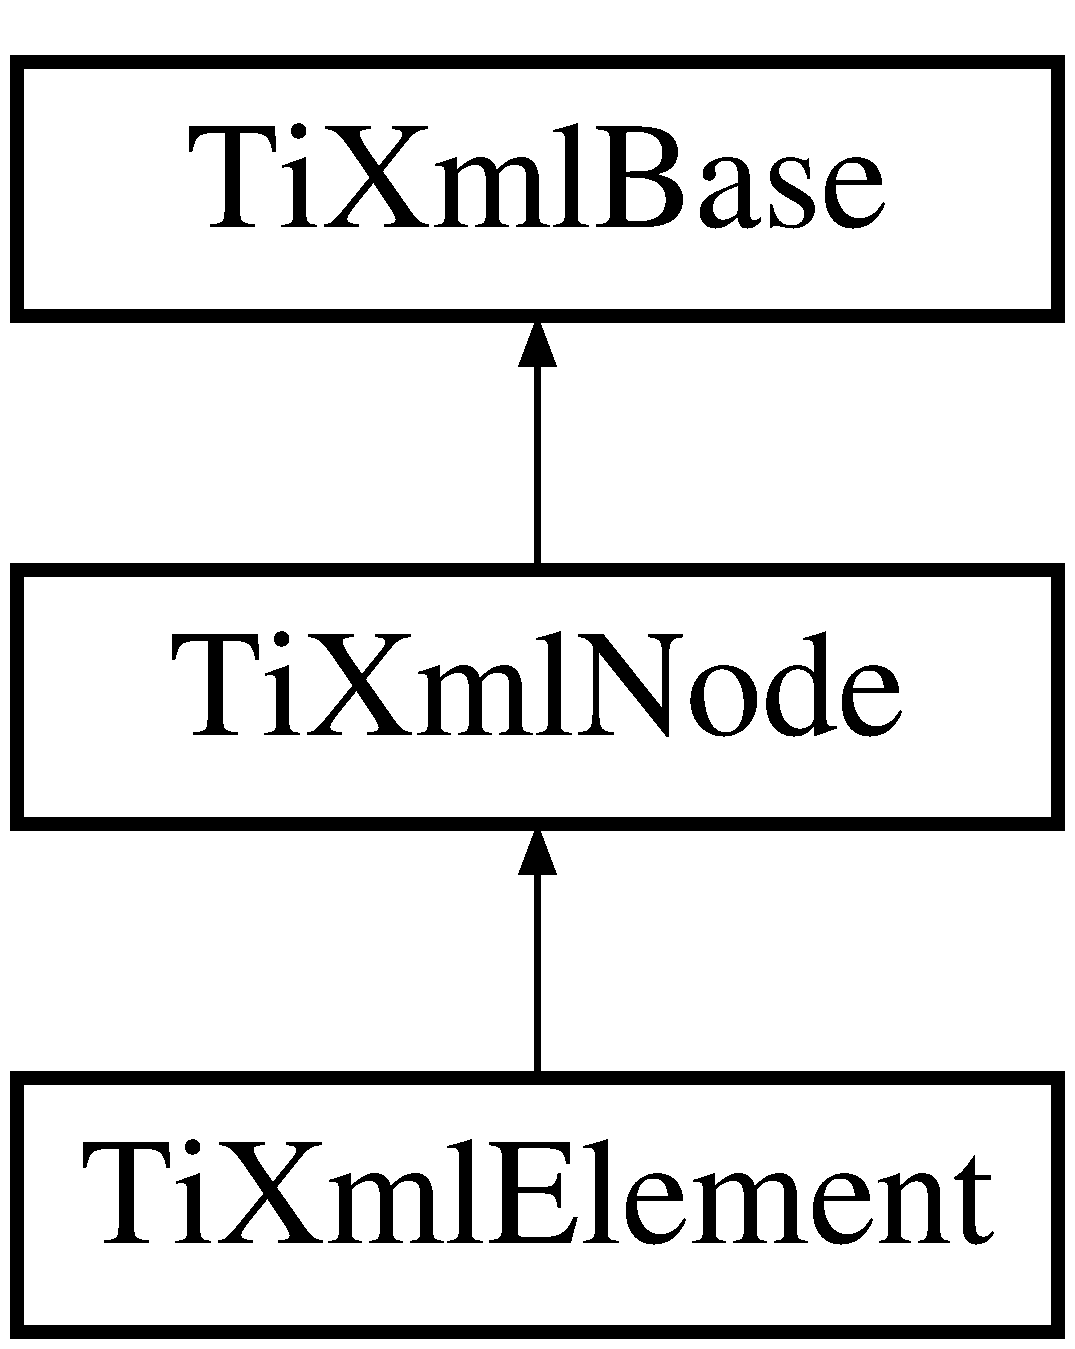
\includegraphics[height=3cm]{classTiXmlElement}
\end{center}
\end{figure}


\subsection{Detailed Description}
The element is a container class. It has a value, the element name, and can contain other elements, text, comments, and unknowns. Elements also contain an arbitrary number of attributes. \subsection*{Public Member Functions}
\begin{CompactItemize}
\item 
{\bf TiXmlElement} (const char $\ast$in\_\-value)
\begin{CompactList}\small\item\em Construct an element. \item\end{CompactList}\item 
{\bf TiXmlElement} (const {\bf TiXmlElement} \&)
\item 
void {\bf operator=} (const {\bf TiXmlElement} \&base)
\item 
virtual {\bf $\sim$TiXmlElement} ()
\item 
const char $\ast$ {\bf Attribute} (const char $\ast$name) const 
\item 
const char $\ast$ {\bf Attribute} (const char $\ast$name, int $\ast$i) const 
\item 
const char $\ast$ {\bf Attribute} (const char $\ast$name, double $\ast$d) const 
\item 
int {\bf QueryIntAttribute} (const char $\ast$name, int $\ast$\_\-value) const 
\item 
int {\bf QueryDoubleAttribute} (const char $\ast$name, double $\ast$\_\-value) const 
\begin{CompactList}\small\item\em QueryDoubleAttribute examines the attribute - see \doxyref{QueryIntAttribute()}{p.}{classTiXmlElement_ea0bfe471380f281c5945770ddbf52b9}. \item\end{CompactList}\item 
int {\bf QueryFloatAttribute} (const char $\ast$name, float $\ast$\_\-value) const 
\begin{CompactList}\small\item\em QueryFloatAttribute examines the attribute - see \doxyref{QueryIntAttribute()}{p.}{classTiXmlElement_ea0bfe471380f281c5945770ddbf52b9}. \item\end{CompactList}\item 
void {\bf SetAttribute} (const char $\ast$name, const char $\ast$\_\-value)
\item 
void {\bf SetAttribute} (const char $\ast$name, int {\bf value})
\item 
void {\bf SetDoubleAttribute} (const char $\ast$name, double {\bf value})
\item 
void {\bf RemoveAttribute} (const char $\ast$name)
\item 
const {\bf TiXmlAttribute} $\ast$ {\bf FirstAttribute} () const 
\begin{CompactList}\small\item\em Access the first attribute in this element. \item\end{CompactList}\item 
{\bf TiXmlAttribute} $\ast$ {\bf FirstAttribute} ()
\item 
const {\bf TiXmlAttribute} $\ast$ {\bf LastAttribute} () const 
\begin{CompactList}\small\item\em Access the last attribute in this element. \item\end{CompactList}\item 
{\bf TiXmlAttribute} $\ast$ {\bf LastAttribute} ()
\item 
const char $\ast$ {\bf GetText} () const 
\item 
virtual {\bf TiXmlNode} $\ast$ {\bf Clone} () const 
\begin{CompactList}\small\item\em Creates a new Element and returns it - the returned element is a copy. \item\end{CompactList}\item 
virtual void {\bf Print} (FILE $\ast$cfile, int depth) const 
\item 
virtual const char $\ast$ {\bf Parse} (const char $\ast$p, {\bf TiXmlParsingData} $\ast$data, {\bf TiXmlEncoding} encoding)
\item 
virtual const {\bf TiXmlElement} $\ast$ {\bf ToElement} () const 
\begin{CompactList}\small\item\em Cast to a more defined type. Will return null not of the requested type. \item\end{CompactList}\item 
virtual {\bf TiXmlElement} $\ast$ {\bf ToElement} ()
\begin{CompactList}\small\item\em Cast to a more defined type. Will return null not of the requested type. \item\end{CompactList}\item 
virtual bool {\bf Accept} ({\bf TiXmlVisitor} $\ast$visitor) const 
\end{CompactItemize}
\subsection*{Protected Member Functions}
\begin{CompactItemize}
\item 
void {\bf CopyTo} ({\bf TiXmlElement} $\ast$target) const 
\item 
void {\bf ClearThis} ()
\item 
const char $\ast$ {\bf ReadValue} (const char $\ast$in, {\bf TiXmlParsingData} $\ast$prevData, {\bf TiXmlEncoding} encoding)
\end{CompactItemize}


\subsection{Constructor \& Destructor Documentation}
\index{TiXmlElement@{TiXmlElement}!TiXmlElement@{TiXmlElement}}
\index{TiXmlElement@{TiXmlElement}!TiXmlElement@{TiXmlElement}}
\subsubsection{\setlength{\rightskip}{0pt plus 5cm}TiXmlElement::TiXmlElement (const char $\ast$ {\em in\_\-value})}\label{classTiXmlElement_01bc3ab372d35da08efcbbe65ad90c60}


Construct an element. 

\index{TiXmlElement@{TiXmlElement}!TiXmlElement@{TiXmlElement}}
\index{TiXmlElement@{TiXmlElement}!TiXmlElement@{TiXmlElement}}
\subsubsection{\setlength{\rightskip}{0pt plus 5cm}TiXmlElement::TiXmlElement (const {\bf TiXmlElement} \& {\em copy})}\label{classTiXmlElement_1ca4465f3c2eac6a60e641cd7f1d9f7e}


\index{TiXmlElement@{TiXmlElement}!$\sim$TiXmlElement@{$\sim$TiXmlElement}}
\index{$\sim$TiXmlElement@{$\sim$TiXmlElement}!TiXmlElement@{TiXmlElement}}
\subsubsection{\setlength{\rightskip}{0pt plus 5cm}TiXmlElement::$\sim$TiXmlElement ()\hspace{0.3cm}{\tt  [virtual]}}\label{classTiXmlElement_a049a47c5081c0d021968666360da261}




\subsection{Member Function Documentation}
\index{TiXmlElement@{TiXmlElement}!operator=@{operator=}}
\index{operator=@{operator=}!TiXmlElement@{TiXmlElement}}
\subsubsection{\setlength{\rightskip}{0pt plus 5cm}void TiXmlElement::operator= (const {\bf TiXmlElement} \& {\em base})}\label{classTiXmlElement_f5cd4156e082ef3bf23adfe0ed173340}


\index{TiXmlElement@{TiXmlElement}!Attribute@{Attribute}}
\index{Attribute@{Attribute}!TiXmlElement@{TiXmlElement}}
\subsubsection{\setlength{\rightskip}{0pt plus 5cm}const char $\ast$ TiXmlElement::Attribute (const char $\ast$ {\em name}) const}\label{classTiXmlElement_c1e4691e9375ba4e665dce7e46a50a9c}


Given an attribute name, \doxyref{Attribute()}{p.}{classTiXmlElement_c1e4691e9375ba4e665dce7e46a50a9c} returns the value for the attribute of that name, or null if none exists. \index{TiXmlElement@{TiXmlElement}!Attribute@{Attribute}}
\index{Attribute@{Attribute}!TiXmlElement@{TiXmlElement}}
\subsubsection{\setlength{\rightskip}{0pt plus 5cm}const char $\ast$ TiXmlElement::Attribute (const char $\ast$ {\em name}, int $\ast$ {\em i}) const}\label{classTiXmlElement_a9192e80567b5042dbded80b78c44339}


Given an attribute name, \doxyref{Attribute()}{p.}{classTiXmlElement_c1e4691e9375ba4e665dce7e46a50a9c} returns the value for the attribute of that name, or null if none exists. If the attribute exists and can be converted to an integer, the integer value will be put in the return 'i', if 'i' is non-null. \index{TiXmlElement@{TiXmlElement}!Attribute@{Attribute}}
\index{Attribute@{Attribute}!TiXmlElement@{TiXmlElement}}
\subsubsection{\setlength{\rightskip}{0pt plus 5cm}const char $\ast$ TiXmlElement::Attribute (const char $\ast$ {\em name}, double $\ast$ {\em d}) const}\label{classTiXmlElement_ec4f727f8aa49b51248d80125d173136}


Given an attribute name, \doxyref{Attribute()}{p.}{classTiXmlElement_c1e4691e9375ba4e665dce7e46a50a9c} returns the value for the attribute of that name, or null if none exists. If the attribute exists and can be converted to an double, the double value will be put in the return 'd', if 'd' is non-null. \index{TiXmlElement@{TiXmlElement}!QueryIntAttribute@{QueryIntAttribute}}
\index{QueryIntAttribute@{QueryIntAttribute}!TiXmlElement@{TiXmlElement}}
\subsubsection{\setlength{\rightskip}{0pt plus 5cm}int TiXmlElement::QueryIntAttribute (const char $\ast$ {\em name}, int $\ast$ {\em \_\-value}) const}\label{classTiXmlElement_ea0bfe471380f281c5945770ddbf52b9}


QueryIntAttribute examines the attribute - it is an alternative to the \doxyref{Attribute()}{p.}{classTiXmlElement_c1e4691e9375ba4e665dce7e46a50a9c} method with richer error checking. If the attribute is an integer, it is stored in 'value' and the call returns TIXML\_\-SUCCESS. If it is not an integer, it returns TIXML\_\-WRONG\_\-TYPE. If the attribute does not exist, then TIXML\_\-NO\_\-ATTRIBUTE is returned. \index{TiXmlElement@{TiXmlElement}!QueryDoubleAttribute@{QueryDoubleAttribute}}
\index{QueryDoubleAttribute@{QueryDoubleAttribute}!TiXmlElement@{TiXmlElement}}
\subsubsection{\setlength{\rightskip}{0pt plus 5cm}int TiXmlElement::QueryDoubleAttribute (const char $\ast$ {\em name}, double $\ast$ {\em \_\-value}) const}\label{classTiXmlElement_898d7730ecc341f0bffc7a9dadbf1ce7}


QueryDoubleAttribute examines the attribute - see \doxyref{QueryIntAttribute()}{p.}{classTiXmlElement_ea0bfe471380f281c5945770ddbf52b9}. 

\index{TiXmlElement@{TiXmlElement}!QueryFloatAttribute@{QueryFloatAttribute}}
\index{QueryFloatAttribute@{QueryFloatAttribute}!TiXmlElement@{TiXmlElement}}
\subsubsection{\setlength{\rightskip}{0pt plus 5cm}int TiXmlElement::QueryFloatAttribute (const char $\ast$ {\em name}, float $\ast$ {\em \_\-value}) const\hspace{0.3cm}{\tt  [inline]}}\label{classTiXmlElement_a04d3af11601ef5a5f88295203a843be}


QueryFloatAttribute examines the attribute - see \doxyref{QueryIntAttribute()}{p.}{classTiXmlElement_ea0bfe471380f281c5945770ddbf52b9}. 

\index{TiXmlElement@{TiXmlElement}!SetAttribute@{SetAttribute}}
\index{SetAttribute@{SetAttribute}!TiXmlElement@{TiXmlElement}}
\subsubsection{\setlength{\rightskip}{0pt plus 5cm}void TiXmlElement::SetAttribute (const char $\ast$ {\em name}, const char $\ast$ {\em \_\-value})}\label{classTiXmlElement_bf0b3bd7f0e4c746a89ec6e7f101fc32}


Sets an attribute of name to a given value. The attribute will be created if it does not exist, or changed if it does. \index{TiXmlElement@{TiXmlElement}!SetAttribute@{SetAttribute}}
\index{SetAttribute@{SetAttribute}!TiXmlElement@{TiXmlElement}}
\subsubsection{\setlength{\rightskip}{0pt plus 5cm}void TiXmlElement::SetAttribute (const char $\ast$ {\em name}, int {\em value})}\label{classTiXmlElement_ce6f4be75e373726d4774073d666d1a7}


Sets an attribute of name to a given value. The attribute will be created if it does not exist, or changed if it does. \index{TiXmlElement@{TiXmlElement}!SetDoubleAttribute@{SetDoubleAttribute}}
\index{SetDoubleAttribute@{SetDoubleAttribute}!TiXmlElement@{TiXmlElement}}
\subsubsection{\setlength{\rightskip}{0pt plus 5cm}void TiXmlElement::SetDoubleAttribute (const char $\ast$ {\em name}, double {\em value})}\label{classTiXmlElement_0d1dd975d75496778177e35abfe0ec0b}


Sets an attribute of name to a given value. The attribute will be created if it does not exist, or changed if it does. \index{TiXmlElement@{TiXmlElement}!RemoveAttribute@{RemoveAttribute}}
\index{RemoveAttribute@{RemoveAttribute}!TiXmlElement@{TiXmlElement}}
\subsubsection{\setlength{\rightskip}{0pt plus 5cm}void TiXmlElement::RemoveAttribute (const char $\ast$ {\em name})}\label{classTiXmlElement_56979767deca794376b1dfa69a525b2a}


Deletes an attribute with the given name. \index{TiXmlElement@{TiXmlElement}!FirstAttribute@{FirstAttribute}}
\index{FirstAttribute@{FirstAttribute}!TiXmlElement@{TiXmlElement}}
\subsubsection{\setlength{\rightskip}{0pt plus 5cm}const {\bf TiXmlAttribute}$\ast$ TiXmlElement::FirstAttribute () const\hspace{0.3cm}{\tt  [inline]}}\label{classTiXmlElement_516054c9073647d6cb29b6abe9fa0592}


Access the first attribute in this element. 

\index{TiXmlElement@{TiXmlElement}!FirstAttribute@{FirstAttribute}}
\index{FirstAttribute@{FirstAttribute}!TiXmlElement@{TiXmlElement}}
\subsubsection{\setlength{\rightskip}{0pt plus 5cm}{\bf TiXmlAttribute}$\ast$ TiXmlElement::FirstAttribute ()\hspace{0.3cm}{\tt  [inline]}}\label{classTiXmlElement_4b33780fc565d38d6b54f640e0cf1737}


\index{TiXmlElement@{TiXmlElement}!LastAttribute@{LastAttribute}}
\index{LastAttribute@{LastAttribute}!TiXmlElement@{TiXmlElement}}
\subsubsection{\setlength{\rightskip}{0pt plus 5cm}const {\bf TiXmlAttribute}$\ast$ TiXmlElement::LastAttribute () const\hspace{0.3cm}{\tt  [inline]}}\label{classTiXmlElement_86191b49f9177be132b85b14655f1381}


Access the last attribute in this element. 

\index{TiXmlElement@{TiXmlElement}!LastAttribute@{LastAttribute}}
\index{LastAttribute@{LastAttribute}!TiXmlElement@{TiXmlElement}}
\subsubsection{\setlength{\rightskip}{0pt plus 5cm}{\bf TiXmlAttribute}$\ast$ TiXmlElement::LastAttribute ()\hspace{0.3cm}{\tt  [inline]}}\label{classTiXmlElement_222f81cf06155cd108f2a68d4d176004}


\index{TiXmlElement@{TiXmlElement}!GetText@{GetText}}
\index{GetText@{GetText}!TiXmlElement@{TiXmlElement}}
\subsubsection{\setlength{\rightskip}{0pt plus 5cm}const char $\ast$ TiXmlElement::GetText () const}\label{classTiXmlElement_a6dedd8a146acf3b1bc0903deb2d411a}


Convenience function for easy access to the text inside an element. Although easy and concise, \doxyref{GetText()}{p.}{classTiXmlElement_a6dedd8a146acf3b1bc0903deb2d411a} is limited compared to getting the \doxyref{TiXmlText}{p.}{classTiXmlText} child and accessing it directly.

If the first child of 'this' is a \doxyref{TiXmlText}{p.}{classTiXmlText}, the \doxyref{GetText()}{p.}{classTiXmlElement_a6dedd8a146acf3b1bc0903deb2d411a} returns the character string of the Text node, else null is returned.

This is a convenient method for getting the text of simple contained text: 

\footnotesize\begin{verbatim}
		<foo>This is text</foo>
		const char* str = fooElement->GetText();
		\end{verbatim}
\normalsize


'str' will be a pointer to \char`\"{}This is text\char`\"{}.

Note that this function can be misleading. If the element foo was created from this XML: 

\footnotesize\begin{verbatim}
		<foo><b>This is text</b></foo> 
		\end{verbatim}
\normalsize


then the value of str would be null. The first child node isn't a text node, it is another element. From this XML: 

\footnotesize\begin{verbatim}
		<foo>This is <b>text</b></foo> 
		\end{verbatim}
\normalsize
 \doxyref{GetText()}{p.}{classTiXmlElement_a6dedd8a146acf3b1bc0903deb2d411a} will return \char`\"{}This is \char`\"{}.

WARNING: \doxyref{GetText()}{p.}{classTiXmlElement_a6dedd8a146acf3b1bc0903deb2d411a} accesses a child node - don't become confused with the similarly named \doxyref{TiXmlHandle::Text()}{p.}{classTiXmlHandle_9fc739c8a18d160006f82572fc143d13} and \doxyref{TiXmlNode::ToText()}{p.}{classTiXmlNode_3ddfbcac78fbea041fad57e5c6d60a03} which are safe type casts on the referenced node. \index{TiXmlElement@{TiXmlElement}!Clone@{Clone}}
\index{Clone@{Clone}!TiXmlElement@{TiXmlElement}}
\subsubsection{\setlength{\rightskip}{0pt plus 5cm}{\bf TiXmlNode} $\ast$ TiXmlElement::Clone () const\hspace{0.3cm}{\tt  [virtual]}}\label{classTiXmlElement_13f6df105ebb1e8dc636e75cc883be32}


Creates a new Element and returns it - the returned element is a copy. 



Implements {\bf TiXmlNode} \doxyref{}{p.}{classTiXmlNode_4508cc3a2d7a98e96a54cc09c37a78a4}.\index{TiXmlElement@{TiXmlElement}!Print@{Print}}
\index{Print@{Print}!TiXmlElement@{TiXmlElement}}
\subsubsection{\setlength{\rightskip}{0pt plus 5cm}void TiXmlElement::Print (FILE $\ast$ {\em cfile}, int {\em depth}) const\hspace{0.3cm}{\tt  [virtual]}}\label{classTiXmlElement_d9d0c008866982ab8d9aafae7e14d692}


All TinyXml classes can print themselves to a filestream or the string class (\doxyref{TiXmlString}{p.}{classTiXmlString} in non-STL mode, std::string in STL mode.) Either or both cfile and str can be null.

This is a formatted print, and will insert tabs and newlines.

(For an unformatted stream, use the $<$$<$ operator.) 

Implements {\bf TiXmlBase} \doxyref{}{p.}{classTiXmlBase_0de56b3f2ef14c65091a3b916437b512}.\index{TiXmlElement@{TiXmlElement}!Parse@{Parse}}
\index{Parse@{Parse}!TiXmlElement@{TiXmlElement}}
\subsubsection{\setlength{\rightskip}{0pt plus 5cm}const char $\ast$ TiXmlElement::Parse (const char $\ast$ {\em p}, {\bf TiXmlParsingData} $\ast$ {\em data}, {\bf TiXmlEncoding} {\em encoding})\hspace{0.3cm}{\tt  [virtual]}}\label{classTiXmlElement_f95c9165159fd9dfdcc5b894a3fcf85b}




Implements {\bf TiXmlBase} \doxyref{}{p.}{classTiXmlBase_00e4edb0219d00a1379c856e5a1d2025}.\index{TiXmlElement@{TiXmlElement}!ToElement@{ToElement}}
\index{ToElement@{ToElement}!TiXmlElement@{TiXmlElement}}
\subsubsection{\setlength{\rightskip}{0pt plus 5cm}virtual const {\bf TiXmlElement}$\ast$ TiXmlElement::ToElement () const\hspace{0.3cm}{\tt  [inline, virtual]}}\label{classTiXmlElement_c5b8d0e25fa23fd9acbb6d146082901c}


Cast to a more defined type. Will return null not of the requested type. 



Reimplemented from {\bf TiXmlNode} \doxyref{}{p.}{classTiXmlNode_72abed96dc9667ab9e0a2a275301bb1c}.\index{TiXmlElement@{TiXmlElement}!ToElement@{ToElement}}
\index{ToElement@{ToElement}!TiXmlElement@{TiXmlElement}}
\subsubsection{\setlength{\rightskip}{0pt plus 5cm}virtual {\bf TiXmlElement}$\ast$ TiXmlElement::ToElement ()\hspace{0.3cm}{\tt  [inline, virtual]}}\label{classTiXmlElement_9def86337ea7a755eb41cac980f60c7a}


Cast to a more defined type. Will return null not of the requested type. 



Reimplemented from {\bf TiXmlNode} \doxyref{}{p.}{classTiXmlNode_a65d000223187d22a4dcebd7479e9ebc}.\index{TiXmlElement@{TiXmlElement}!Accept@{Accept}}
\index{Accept@{Accept}!TiXmlElement@{TiXmlElement}}
\subsubsection{\setlength{\rightskip}{0pt plus 5cm}bool TiXmlElement::Accept ({\bf TiXmlVisitor} $\ast$ {\em visitor}) const\hspace{0.3cm}{\tt  [virtual]}}\label{classTiXmlElement_31ab28cc3b892a69254391d6bbe08df3}


Walk the XML tree visiting this node and all of its children. 

Implements {\bf TiXmlNode} \doxyref{}{p.}{classTiXmlNode_cc0f88b7462c6cb73809d410a4f5bb86}.\index{TiXmlElement@{TiXmlElement}!CopyTo@{CopyTo}}
\index{CopyTo@{CopyTo}!TiXmlElement@{TiXmlElement}}
\subsubsection{\setlength{\rightskip}{0pt plus 5cm}void TiXmlElement::CopyTo ({\bf TiXmlElement} $\ast$ {\em target}) const\hspace{0.3cm}{\tt  [protected]}}\label{classTiXmlElement_9e0c1983b840de4134f1f6bf7af00b0f}


\index{TiXmlElement@{TiXmlElement}!ClearThis@{ClearThis}}
\index{ClearThis@{ClearThis}!TiXmlElement@{TiXmlElement}}
\subsubsection{\setlength{\rightskip}{0pt plus 5cm}void TiXmlElement::ClearThis ()\hspace{0.3cm}{\tt  [protected]}}\label{classTiXmlElement_5670933ec2d7d9763b9891acc05d7f7d}


\index{TiXmlElement@{TiXmlElement}!ReadValue@{ReadValue}}
\index{ReadValue@{ReadValue}!TiXmlElement@{TiXmlElement}}
\subsubsection{\setlength{\rightskip}{0pt plus 5cm}const char $\ast$ TiXmlElement::ReadValue (const char $\ast$ {\em in}, {\bf TiXmlParsingData} $\ast$ {\em prevData}, {\bf TiXmlEncoding} {\em encoding})\hspace{0.3cm}{\tt  [protected]}}\label{classTiXmlElement_c786bce103042d3837c4cc2ff6967d41}




The documentation for this class was generated from the following files:\begin{CompactItemize}
\item 
/home/msneddon/eclipse/galileoSR1\_\-cpp/workspace/NFsim/src/NFinput/TinyXML/{\bf tinyxml.h}\item 
/home/msneddon/eclipse/galileoSR1\_\-cpp/workspace/NFsim/src/NFinput/TinyXML/{\bf tinyxml.cpp}\item 
/home/msneddon/eclipse/galileoSR1\_\-cpp/workspace/NFsim/src/NFinput/TinyXML/{\bf tinyxmlparser.cpp}\end{CompactItemize}

\section{TiXmlHandle Class Reference}
\label{classTiXmlHandle}\index{TiXmlHandle@{TiXmlHandle}}
{\tt \#include $<$tinyxml.h$>$}



\subsection{Detailed Description}
A \doxyref{TiXmlHandle}{p.}{classTiXmlHandle} is a class that wraps a node pointer with null checks; this is an incredibly useful thing. Note that \doxyref{TiXmlHandle}{p.}{classTiXmlHandle} is not part of the TinyXml DOM structure. It is a separate utility class.

Take an example: 

\footnotesize\begin{verbatim}
	<Document>
		<Element attributeA = "valueA">
			<Child attributeB = "value1" />
			<Child attributeB = "value2" />
		</Element>
	<Document>
	\end{verbatim}
\normalsize


Assuming you want the value of \char`\"{}attributeB\char`\"{} in the 2nd \char`\"{}Child\char`\"{} element, it's very easy to write a $\ast$lot$\ast$ of code that looks like:



\footnotesize\begin{verbatim}
	TiXmlElement* root = document.FirstChildElement( "Document" );
	if ( root )
	{
		TiXmlElement* element = root->FirstChildElement( "Element" );
		if ( element )
		{
			TiXmlElement* child = element->FirstChildElement( "Child" );
			if ( child )
			{
				TiXmlElement* child2 = child->NextSiblingElement( "Child" );
				if ( child2 )
				{
					// Finally do something useful.
	\end{verbatim}
\normalsize


And that doesn't even cover \char`\"{}else\char`\"{} cases. \doxyref{TiXmlHandle}{p.}{classTiXmlHandle} addresses the verbosity of such code. A \doxyref{TiXmlHandle}{p.}{classTiXmlHandle} checks for null pointers so it is perfectly safe and correct to use:



\footnotesize\begin{verbatim}
	TiXmlHandle docHandle( &document );
	TiXmlElement* child2 = docHandle.FirstChild( "Document" ).FirstChild( "Element" ).Child( "Child", 1 ).ToElement();
	if ( child2 )
	{
		// do something useful
	\end{verbatim}
\normalsize


Which is MUCH more concise and useful.

It is also safe to copy handles - internally they are nothing more than node pointers. 

\footnotesize\begin{verbatim}
	TiXmlHandle handleCopy = handle;
	\end{verbatim}
\normalsize


What they should not be used for is iteration:



\footnotesize\begin{verbatim}
	int i=0; 
	while ( true )
	{
		TiXmlElement* child = docHandle.FirstChild( "Document" ).FirstChild( "Element" ).Child( "Child", i ).ToElement();
		if ( !child )
			break;
		// do something
		++i;
	}
	\end{verbatim}
\normalsize


It seems reasonable, but it is in fact two embedded while loops. The Child method is a linear walk to find the element, so this code would iterate much more than it needs to. Instead, prefer:



\footnotesize\begin{verbatim}
	TiXmlElement* child = docHandle.FirstChild( "Document" ).FirstChild( "Element" ).FirstChild( "Child" ).ToElement();

	for( child; child; child=child->NextSiblingElement() )
	{
		// do something
	}
	\end{verbatim}
\normalsize
 \subsection*{Public Member Functions}
\begin{CompactItemize}
\item 
{\bf TiXmlHandle} ({\bf TiXmlNode} $\ast$\_\-node)
\begin{CompactList}\small\item\em Create a handle from any node (at any depth of the tree.) This can be a null pointer. \item\end{CompactList}\item 
{\bf TiXmlHandle} (const {\bf TiXmlHandle} \&ref)
\begin{CompactList}\small\item\em Copy constructor. \item\end{CompactList}\item 
{\bf TiXmlHandle} {\bf operator=} (const {\bf TiXmlHandle} \&ref)
\item 
{\bf TiXmlHandle} {\bf FirstChild} () const 
\begin{CompactList}\small\item\em Return a handle to the first child node. \item\end{CompactList}\item 
{\bf TiXmlHandle} {\bf FirstChild} (const char $\ast$value) const 
\begin{CompactList}\small\item\em Return a handle to the first child node with the given name. \item\end{CompactList}\item 
{\bf TiXmlHandle} {\bf FirstChildElement} () const 
\begin{CompactList}\small\item\em Return a handle to the first child element. \item\end{CompactList}\item 
{\bf TiXmlHandle} {\bf FirstChildElement} (const char $\ast$value) const 
\begin{CompactList}\small\item\em Return a handle to the first child element with the given name. \item\end{CompactList}\item 
{\bf TiXmlHandle} {\bf Child} (const char $\ast$value, int index) const 
\item 
{\bf TiXmlHandle} {\bf Child} (int index) const 
\item 
{\bf TiXmlHandle} {\bf ChildElement} (const char $\ast$value, int index) const 
\item 
{\bf TiXmlHandle} {\bf ChildElement} (int index) const 
\item 
{\bf TiXmlNode} $\ast$ {\bf ToNode} () const 
\item 
{\bf TiXmlElement} $\ast$ {\bf ToElement} () const 
\item 
{\bf TiXmlText} $\ast$ {\bf ToText} () const 
\item 
{\bf TiXmlUnknown} $\ast$ {\bf ToUnknown} () const 
\item 
{\bf TiXmlNode} $\ast$ {\bf Node} () const 
\item 
{\bf TiXmlElement} $\ast$ {\bf Element} () const 
\item 
{\bf TiXmlText} $\ast$ {\bf Text} () const 
\item 
{\bf TiXmlUnknown} $\ast$ {\bf Unknown} () const 
\end{CompactItemize}


\subsection{Constructor \& Destructor Documentation}
\index{TiXmlHandle@{TiXmlHandle}!TiXmlHandle@{TiXmlHandle}}
\index{TiXmlHandle@{TiXmlHandle}!TiXmlHandle@{TiXmlHandle}}
\subsubsection{\setlength{\rightskip}{0pt plus 5cm}TiXmlHandle::TiXmlHandle ({\bf TiXmlNode} $\ast$ {\em \_\-node})\hspace{0.3cm}{\tt  [inline]}}\label{classTiXmlHandle_ba18fd7bdefb942ecdea4bf4b8e29ec8}


Create a handle from any node (at any depth of the tree.) This can be a null pointer. 

\index{TiXmlHandle@{TiXmlHandle}!TiXmlHandle@{TiXmlHandle}}
\index{TiXmlHandle@{TiXmlHandle}!TiXmlHandle@{TiXmlHandle}}
\subsubsection{\setlength{\rightskip}{0pt plus 5cm}TiXmlHandle::TiXmlHandle (const {\bf TiXmlHandle} \& {\em ref})\hspace{0.3cm}{\tt  [inline]}}\label{classTiXmlHandle_236d7855e1e56ccc7b980630c48c7fd7}


Copy constructor. 



\subsection{Member Function Documentation}
\index{TiXmlHandle@{TiXmlHandle}!operator=@{operator=}}
\index{operator=@{operator=}!TiXmlHandle@{TiXmlHandle}}
\subsubsection{\setlength{\rightskip}{0pt plus 5cm}{\bf TiXmlHandle} TiXmlHandle::operator= (const {\bf TiXmlHandle} \& {\em ref})\hspace{0.3cm}{\tt  [inline]}}\label{classTiXmlHandle_d8e5dcf6a87882674203157f29f8e4db}


\index{TiXmlHandle@{TiXmlHandle}!FirstChild@{FirstChild}}
\index{FirstChild@{FirstChild}!TiXmlHandle@{TiXmlHandle}}
\subsubsection{\setlength{\rightskip}{0pt plus 5cm}{\bf TiXmlHandle} TiXmlHandle::FirstChild () const}\label{classTiXmlHandle_cdb1faaf88a700b40ca2c8d9aee21139}


Return a handle to the first child node. 

\index{TiXmlHandle@{TiXmlHandle}!FirstChild@{FirstChild}}
\index{FirstChild@{FirstChild}!TiXmlHandle@{TiXmlHandle}}
\subsubsection{\setlength{\rightskip}{0pt plus 5cm}{\bf TiXmlHandle} TiXmlHandle::FirstChild (const char $\ast$ {\em value}) const}\label{classTiXmlHandle_8c61f64ae9365d89c264f289085541f8}


Return a handle to the first child node with the given name. 

\index{TiXmlHandle@{TiXmlHandle}!FirstChildElement@{FirstChildElement}}
\index{FirstChildElement@{FirstChildElement}!TiXmlHandle@{TiXmlHandle}}
\subsubsection{\setlength{\rightskip}{0pt plus 5cm}{\bf TiXmlHandle} TiXmlHandle::FirstChildElement () const}\label{classTiXmlHandle_24d1112e995e937e4dddb202d4113d4a}


Return a handle to the first child element. 

\index{TiXmlHandle@{TiXmlHandle}!FirstChildElement@{FirstChildElement}}
\index{FirstChildElement@{FirstChildElement}!TiXmlHandle@{TiXmlHandle}}
\subsubsection{\setlength{\rightskip}{0pt plus 5cm}{\bf TiXmlHandle} TiXmlHandle::FirstChildElement (const char $\ast$ {\em value}) const}\label{classTiXmlHandle_f0aea751320f5e430fac6f8fff3b8dd4}


Return a handle to the first child element with the given name. 

\index{TiXmlHandle@{TiXmlHandle}!Child@{Child}}
\index{Child@{Child}!TiXmlHandle@{TiXmlHandle}}
\subsubsection{\setlength{\rightskip}{0pt plus 5cm}{\bf TiXmlHandle} TiXmlHandle::Child (const char $\ast$ {\em value}, int {\em index}) const}\label{classTiXmlHandle_072492b4be1acdb0db2d03cd8f71ccc4}


Return a handle to the \char`\"{}index\char`\"{} child with the given name. The first child is 0, the second 1, etc. \index{TiXmlHandle@{TiXmlHandle}!Child@{Child}}
\index{Child@{Child}!TiXmlHandle@{TiXmlHandle}}
\subsubsection{\setlength{\rightskip}{0pt plus 5cm}{\bf TiXmlHandle} TiXmlHandle::Child (int {\em index}) const}\label{classTiXmlHandle_f9cf6a7d08a5da94a8924425ad0cd5ac}


Return a handle to the \char`\"{}index\char`\"{} child. The first child is 0, the second 1, etc. \index{TiXmlHandle@{TiXmlHandle}!ChildElement@{ChildElement}}
\index{ChildElement@{ChildElement}!TiXmlHandle@{TiXmlHandle}}
\subsubsection{\setlength{\rightskip}{0pt plus 5cm}{\bf TiXmlHandle} TiXmlHandle::ChildElement (const char $\ast$ {\em value}, int {\em index}) const}\label{classTiXmlHandle_979a3f850984a176ee884e394c7eed2d}


Return a handle to the \char`\"{}index\char`\"{} child element with the given name. The first child element is 0, the second 1, etc. Note that only TiXmlElements are indexed: other types are not counted. \index{TiXmlHandle@{TiXmlHandle}!ChildElement@{ChildElement}}
\index{ChildElement@{ChildElement}!TiXmlHandle@{TiXmlHandle}}
\subsubsection{\setlength{\rightskip}{0pt plus 5cm}{\bf TiXmlHandle} TiXmlHandle::ChildElement (int {\em index}) const}\label{classTiXmlHandle_8786475b9d1f1518492e3a46704c7ef0}


Return a handle to the \char`\"{}index\char`\"{} child element. The first child element is 0, the second 1, etc. Note that only TiXmlElements are indexed: other types are not counted. \index{TiXmlHandle@{TiXmlHandle}!ToNode@{ToNode}}
\index{ToNode@{ToNode}!TiXmlHandle@{TiXmlHandle}}
\subsubsection{\setlength{\rightskip}{0pt plus 5cm}{\bf TiXmlNode}$\ast$ TiXmlHandle::ToNode () const\hspace{0.3cm}{\tt  [inline]}}\label{classTiXmlHandle_f678e5088e83be67baf76f699756f2c3}


Return the handle as a \doxyref{TiXmlNode}{p.}{classTiXmlNode}. This may return null. \index{TiXmlHandle@{TiXmlHandle}!ToElement@{ToElement}}
\index{ToElement@{ToElement}!TiXmlHandle@{TiXmlHandle}}
\subsubsection{\setlength{\rightskip}{0pt plus 5cm}{\bf TiXmlElement}$\ast$ TiXmlHandle::ToElement () const\hspace{0.3cm}{\tt  [inline]}}\label{classTiXmlHandle_bc6e7ed383a5fe1e52b0c0004b457b9e}


Return the handle as a \doxyref{TiXmlElement}{p.}{classTiXmlElement}. This may return null. \index{TiXmlHandle@{TiXmlHandle}!ToText@{ToText}}
\index{ToText@{ToText}!TiXmlHandle@{TiXmlHandle}}
\subsubsection{\setlength{\rightskip}{0pt plus 5cm}{\bf TiXmlText}$\ast$ TiXmlHandle::ToText () const\hspace{0.3cm}{\tt  [inline]}}\label{classTiXmlHandle_4ac53a652296203a5b5e13854d923586}


Return the handle as a \doxyref{TiXmlText}{p.}{classTiXmlText}. This may return null. \index{TiXmlHandle@{TiXmlHandle}!ToUnknown@{ToUnknown}}
\index{ToUnknown@{ToUnknown}!TiXmlHandle@{TiXmlHandle}}
\subsubsection{\setlength{\rightskip}{0pt plus 5cm}{\bf TiXmlUnknown}$\ast$ TiXmlHandle::ToUnknown () const\hspace{0.3cm}{\tt  [inline]}}\label{classTiXmlHandle_1381c17507a130767b1e23afc93b3674}


Return the handle as a \doxyref{TiXmlUnknown}{p.}{classTiXmlUnknown}. This may return null. \index{TiXmlHandle@{TiXmlHandle}!Node@{Node}}
\index{Node@{Node}!TiXmlHandle@{TiXmlHandle}}
\subsubsection{\setlength{\rightskip}{0pt plus 5cm}{\bf TiXmlNode}$\ast$ TiXmlHandle::Node () const\hspace{0.3cm}{\tt  [inline]}}\label{classTiXmlHandle_b44b723a8dc9af72838a303c079d0376}


\begin{Desc}
\item[{\bf Deprecated}]use ToNode. Return the handle as a \doxyref{TiXmlNode}{p.}{classTiXmlNode}. This may return null. \end{Desc}
\index{TiXmlHandle@{TiXmlHandle}!Element@{Element}}
\index{Element@{Element}!TiXmlHandle@{TiXmlHandle}}
\subsubsection{\setlength{\rightskip}{0pt plus 5cm}{\bf TiXmlElement}$\ast$ TiXmlHandle::Element () const\hspace{0.3cm}{\tt  [inline]}}\label{classTiXmlHandle_cb5fe8388a526289ea65e817a51e05e7}


\begin{Desc}
\item[{\bf Deprecated}]use ToElement. Return the handle as a \doxyref{TiXmlElement}{p.}{classTiXmlElement}. This may return null. \end{Desc}
\index{TiXmlHandle@{TiXmlHandle}!Text@{Text}}
\index{Text@{Text}!TiXmlHandle@{TiXmlHandle}}
\subsubsection{\setlength{\rightskip}{0pt plus 5cm}{\bf TiXmlText}$\ast$ TiXmlHandle::Text () const\hspace{0.3cm}{\tt  [inline]}}\label{classTiXmlHandle_9fc739c8a18d160006f82572fc143d13}


\begin{Desc}
\item[{\bf Deprecated}]use \doxyref{ToText()}{p.}{classTiXmlHandle_4ac53a652296203a5b5e13854d923586} Return the handle as a \doxyref{TiXmlText}{p.}{classTiXmlText}. This may return null. \end{Desc}
\index{TiXmlHandle@{TiXmlHandle}!Unknown@{Unknown}}
\index{Unknown@{Unknown}!TiXmlHandle@{TiXmlHandle}}
\subsubsection{\setlength{\rightskip}{0pt plus 5cm}{\bf TiXmlUnknown}$\ast$ TiXmlHandle::Unknown () const\hspace{0.3cm}{\tt  [inline]}}\label{classTiXmlHandle_49675b74357ba2aae124657a9a1ef465}


\begin{Desc}
\item[{\bf Deprecated}]use \doxyref{ToUnknown()}{p.}{classTiXmlHandle_1381c17507a130767b1e23afc93b3674} Return the handle as a \doxyref{TiXmlUnknown}{p.}{classTiXmlUnknown}. This may return null. \end{Desc}


The documentation for this class was generated from the following files:\begin{CompactItemize}
\item 
/home/msneddon/eclipse/ganymede\_\-cpp/workspace/NFsim\_\-svn/src/NFinput/TinyXML/{\bf tinyxml.h}\item 
/home/msneddon/eclipse/ganymede\_\-cpp/workspace/NFsim\_\-svn/src/NFinput/TinyXML/{\bf tinyxml.cpp}\end{CompactItemize}

\section{TiXmlNode Class Reference}
\label{classTiXmlNode}\index{TiXmlNode@{TiXmlNode}}
{\tt \#include $<$tinyxml.h$>$}

Inheritance diagram for TiXmlNode::\begin{figure}[H]
\begin{center}
\leavevmode
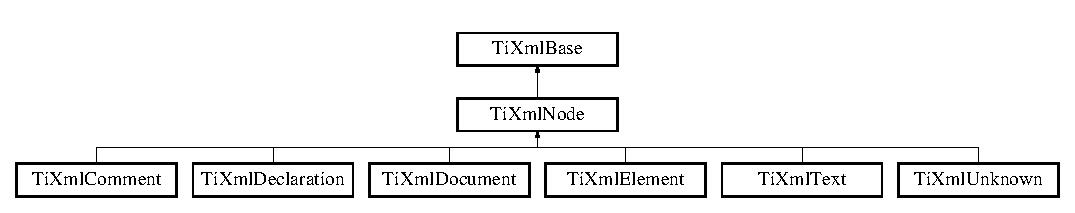
\includegraphics[height=2.41379cm]{classTiXmlNode}
\end{center}
\end{figure}


\subsection{Detailed Description}
The parent class for everything in the Document Object Model. (Except for attributes). Nodes have siblings, a parent, and children. A node can be in a document, or stand on its own. The type of a \doxyref{TiXmlNode}{p.}{classTiXmlNode} can be queried, and it can be cast to its more defined type. \subsection*{Public Types}
\begin{CompactItemize}
\item 
enum {\bf NodeType} \{ \par
{\bf DOCUMENT}, 
{\bf ELEMENT}, 
{\bf COMMENT}, 
{\bf UNKNOWN}, 
\par
{\bf TEXT}, 
{\bf DECLARATION}, 
{\bf TYPECOUNT}
 \}
\end{CompactItemize}
\subsection*{Public Member Functions}
\begin{CompactItemize}
\item 
virtual {\bf $\sim$TiXmlNode} ()
\item 
const char $\ast$ {\bf Value} () const 
\item 
const TIXML\_\-STRING \& {\bf ValueTStr} () const 
\item 
void {\bf SetValue} (const char $\ast$\_\-value)
\item 
void {\bf Clear} ()
\begin{CompactList}\small\item\em Delete all the children of this node. Does not affect 'this'. \item\end{CompactList}\item 
{\bf TiXmlNode} $\ast$ {\bf Parent} ()
\begin{CompactList}\small\item\em One step up the DOM. \item\end{CompactList}\item 
const {\bf TiXmlNode} $\ast$ {\bf Parent} () const 
\item 
const {\bf TiXmlNode} $\ast$ {\bf FirstChild} () const 
\begin{CompactList}\small\item\em The first child of this node. Will be null if there are no children. \item\end{CompactList}\item 
{\bf TiXmlNode} $\ast$ {\bf FirstChild} ()
\item 
const {\bf TiXmlNode} $\ast$ {\bf FirstChild} (const char $\ast${\bf value}) const 
\item 
{\bf TiXmlNode} $\ast$ {\bf FirstChild} (const char $\ast$\_\-value)
\begin{CompactList}\small\item\em The first child of this node with the matching 'value'. Will be null if none found. \item\end{CompactList}\item 
const {\bf TiXmlNode} $\ast$ {\bf LastChild} () const 
\item 
{\bf TiXmlNode} $\ast$ {\bf LastChild} ()
\begin{CompactList}\small\item\em The last child of this node. Will be null if there are no children. \item\end{CompactList}\item 
const {\bf TiXmlNode} $\ast$ {\bf LastChild} (const char $\ast${\bf value}) const 
\item 
{\bf TiXmlNode} $\ast$ {\bf LastChild} (const char $\ast$\_\-value)
\begin{CompactList}\small\item\em The last child of this node matching 'value'. Will be null if there are no children. \item\end{CompactList}\item 
const {\bf TiXmlNode} $\ast$ {\bf IterateChildren} (const {\bf TiXmlNode} $\ast$previous) const 
\item 
{\bf TiXmlNode} $\ast$ {\bf IterateChildren} (const {\bf TiXmlNode} $\ast$previous)
\item 
const {\bf TiXmlNode} $\ast$ {\bf IterateChildren} (const char $\ast${\bf value}, const {\bf TiXmlNode} $\ast$previous) const 
\begin{CompactList}\small\item\em This flavor of IterateChildren searches for children with a particular 'value'. \item\end{CompactList}\item 
{\bf TiXmlNode} $\ast$ {\bf IterateChildren} (const char $\ast$\_\-value, const {\bf TiXmlNode} $\ast$previous)
\item 
{\bf TiXmlNode} $\ast$ {\bf InsertEndChild} (const {\bf TiXmlNode} \&addThis)
\item 
{\bf TiXmlNode} $\ast$ {\bf LinkEndChild} ({\bf TiXmlNode} $\ast$addThis)
\item 
{\bf TiXmlNode} $\ast$ {\bf InsertBeforeChild} ({\bf TiXmlNode} $\ast$beforeThis, const {\bf TiXmlNode} \&addThis)
\item 
{\bf TiXmlNode} $\ast$ {\bf InsertAfterChild} ({\bf TiXmlNode} $\ast$afterThis, const {\bf TiXmlNode} \&addThis)
\item 
{\bf TiXmlNode} $\ast$ {\bf ReplaceChild} ({\bf TiXmlNode} $\ast$replaceThis, const {\bf TiXmlNode} \&withThis)
\item 
bool {\bf RemoveChild} ({\bf TiXmlNode} $\ast$removeThis)
\begin{CompactList}\small\item\em Delete a child of this node. \item\end{CompactList}\item 
const {\bf TiXmlNode} $\ast$ {\bf PreviousSibling} () const 
\begin{CompactList}\small\item\em Navigate to a sibling node. \item\end{CompactList}\item 
{\bf TiXmlNode} $\ast$ {\bf PreviousSibling} ()
\item 
const {\bf TiXmlNode} $\ast$ {\bf PreviousSibling} (const char $\ast$) const 
\begin{CompactList}\small\item\em Navigate to a sibling node. \item\end{CompactList}\item 
{\bf TiXmlNode} $\ast$ {\bf PreviousSibling} (const char $\ast$\_\-prev)
\item 
const {\bf TiXmlNode} $\ast$ {\bf NextSibling} () const 
\begin{CompactList}\small\item\em Navigate to a sibling node. \item\end{CompactList}\item 
{\bf TiXmlNode} $\ast$ {\bf NextSibling} ()
\item 
const {\bf TiXmlNode} $\ast$ {\bf NextSibling} (const char $\ast$) const 
\begin{CompactList}\small\item\em Navigate to a sibling node with the given 'value'. \item\end{CompactList}\item 
{\bf TiXmlNode} $\ast$ {\bf NextSibling} (const char $\ast$\_\-next)
\item 
const {\bf TiXmlElement} $\ast$ {\bf NextSiblingElement} () const 
\item 
{\bf TiXmlElement} $\ast$ {\bf NextSiblingElement} ()
\item 
const {\bf TiXmlElement} $\ast$ {\bf NextSiblingElement} (const char $\ast$) const 
\item 
{\bf TiXmlElement} $\ast$ {\bf NextSiblingElement} (const char $\ast$\_\-next)
\item 
const {\bf TiXmlElement} $\ast$ {\bf FirstChildElement} () const 
\begin{CompactList}\small\item\em Convenience function to get through elements. \item\end{CompactList}\item 
{\bf TiXmlElement} $\ast$ {\bf FirstChildElement} ()
\item 
const {\bf TiXmlElement} $\ast$ {\bf FirstChildElement} (const char $\ast$\_\-value) const 
\begin{CompactList}\small\item\em Convenience function to get through elements. \item\end{CompactList}\item 
{\bf TiXmlElement} $\ast$ {\bf FirstChildElement} (const char $\ast$\_\-value)
\item 
int {\bf Type} () const 
\item 
const {\bf TiXmlDocument} $\ast$ {\bf GetDocument} () const 
\item 
{\bf TiXmlDocument} $\ast$ {\bf GetDocument} ()
\item 
bool {\bf NoChildren} () const 
\begin{CompactList}\small\item\em Returns true if this node has no children. \item\end{CompactList}\item 
virtual const {\bf TiXmlDocument} $\ast$ {\bf ToDocument} () const 
\begin{CompactList}\small\item\em Cast to a more defined type. Will return null if not of the requested type. \item\end{CompactList}\item 
virtual const {\bf TiXmlElement} $\ast$ {\bf ToElement} () const 
\begin{CompactList}\small\item\em Cast to a more defined type. Will return null if not of the requested type. \item\end{CompactList}\item 
virtual const {\bf TiXmlComment} $\ast$ {\bf ToComment} () const 
\begin{CompactList}\small\item\em Cast to a more defined type. Will return null if not of the requested type. \item\end{CompactList}\item 
virtual const {\bf TiXmlUnknown} $\ast$ {\bf ToUnknown} () const 
\begin{CompactList}\small\item\em Cast to a more defined type. Will return null if not of the requested type. \item\end{CompactList}\item 
virtual const {\bf TiXmlText} $\ast$ {\bf ToText} () const 
\begin{CompactList}\small\item\em Cast to a more defined type. Will return null if not of the requested type. \item\end{CompactList}\item 
virtual const {\bf TiXmlDeclaration} $\ast$ {\bf ToDeclaration} () const 
\begin{CompactList}\small\item\em Cast to a more defined type. Will return null if not of the requested type. \item\end{CompactList}\item 
virtual {\bf TiXmlDocument} $\ast$ {\bf ToDocument} ()
\begin{CompactList}\small\item\em Cast to a more defined type. Will return null if not of the requested type. \item\end{CompactList}\item 
virtual {\bf TiXmlElement} $\ast$ {\bf ToElement} ()
\begin{CompactList}\small\item\em Cast to a more defined type. Will return null if not of the requested type. \item\end{CompactList}\item 
virtual {\bf TiXmlComment} $\ast$ {\bf ToComment} ()
\begin{CompactList}\small\item\em Cast to a more defined type. Will return null if not of the requested type. \item\end{CompactList}\item 
virtual {\bf TiXmlUnknown} $\ast$ {\bf ToUnknown} ()
\begin{CompactList}\small\item\em Cast to a more defined type. Will return null if not of the requested type. \item\end{CompactList}\item 
virtual {\bf TiXmlText} $\ast$ {\bf ToText} ()
\begin{CompactList}\small\item\em Cast to a more defined type. Will return null if not of the requested type. \item\end{CompactList}\item 
virtual {\bf TiXmlDeclaration} $\ast$ {\bf ToDeclaration} ()
\begin{CompactList}\small\item\em Cast to a more defined type. Will return null if not of the requested type. \item\end{CompactList}\item 
virtual {\bf TiXmlNode} $\ast$ {\bf Clone} () const =0
\item 
virtual bool {\bf Accept} ({\bf TiXmlVisitor} $\ast$visitor) const =0
\end{CompactItemize}
\subsection*{Protected Member Functions}
\begin{CompactItemize}
\item 
{\bf TiXmlNode} ({\bf NodeType} \_\-type)
\item 
void {\bf CopyTo} ({\bf TiXmlNode} $\ast$target) const 
\item 
{\bf TiXmlNode} $\ast$ {\bf Identify} (const char $\ast$start, {\bf TiXmlEncoding} encoding)
\end{CompactItemize}
\subsection*{Protected Attributes}
\begin{CompactItemize}
\item 
{\bf TiXmlNode} $\ast$ {\bf parent}
\item 
{\bf NodeType} {\bf type}
\item 
{\bf TiXmlNode} $\ast$ {\bf firstChild}
\item 
{\bf TiXmlNode} $\ast$ {\bf lastChild}
\item 
TIXML\_\-STRING {\bf value}
\item 
{\bf TiXmlNode} $\ast$ {\bf prev}
\item 
{\bf TiXmlNode} $\ast$ {\bf next}
\end{CompactItemize}
\subsection*{Friends}
\begin{CompactItemize}
\item 
class {\bf TiXmlDocument}
\item 
class {\bf TiXmlElement}
\end{CompactItemize}


\subsection{Member Enumeration Documentation}
\index{TiXmlNode@{TiXmlNode}!NodeType@{NodeType}}
\index{NodeType@{NodeType}!TiXmlNode@{TiXmlNode}}
\subsubsection{\setlength{\rightskip}{0pt plus 5cm}enum {\bf TiXmlNode::NodeType}}\label{classTiXmlNode_836eded4920ab9e9ef28496f48cd95a2}


The types of XML nodes supported by TinyXml. (All the unsupported types are picked up by UNKNOWN.) \begin{Desc}
\item[Enumerator: ]\par
\begin{description}
\index{DOCUMENT@{DOCUMENT}!TiXmlNode@{TiXmlNode}}\index{TiXmlNode@{TiXmlNode}!DOCUMENT@{DOCUMENT}}\item[{\em 
DOCUMENT\label{classTiXmlNode_836eded4920ab9e9ef28496f48cd95a231b8d14e0558445bb40e36a532b24127}
}]\index{ELEMENT@{ELEMENT}!TiXmlNode@{TiXmlNode}}\index{TiXmlNode@{TiXmlNode}!ELEMENT@{ELEMENT}}\item[{\em 
ELEMENT\label{classTiXmlNode_836eded4920ab9e9ef28496f48cd95a2af2344bcea122ef52d47c4dcc357f070}
}]\index{COMMENT@{COMMENT}!TiXmlNode@{TiXmlNode}}\index{TiXmlNode@{TiXmlNode}!COMMENT@{COMMENT}}\item[{\em 
COMMENT\label{classTiXmlNode_836eded4920ab9e9ef28496f48cd95a27737f35757c7152ca4f612d449ea0e4b}
}]\index{UNKNOWN@{UNKNOWN}!TiXmlNode@{TiXmlNode}}\index{TiXmlNode@{TiXmlNode}!UNKNOWN@{UNKNOWN}}\item[{\em 
UNKNOWN\label{classTiXmlNode_836eded4920ab9e9ef28496f48cd95a2f521ee2fb1e05705776b28fc55a70037}
}]\index{TEXT@{TEXT}!TiXmlNode@{TiXmlNode}}\index{TiXmlNode@{TiXmlNode}!TEXT@{TEXT}}\item[{\em 
TEXT\label{classTiXmlNode_836eded4920ab9e9ef28496f48cd95a2672617f36c5606a966ac378e6ddc0fd8}
}]\index{DECLARATION@{DECLARATION}!TiXmlNode@{TiXmlNode}}\index{TiXmlNode@{TiXmlNode}!DECLARATION@{DECLARATION}}\item[{\em 
DECLARATION\label{classTiXmlNode_836eded4920ab9e9ef28496f48cd95a2c02445686c2b72d11385002b3466c28b}
}]\index{TYPECOUNT@{TYPECOUNT}!TiXmlNode@{TiXmlNode}}\index{TiXmlNode@{TiXmlNode}!TYPECOUNT@{TYPECOUNT}}\item[{\em 
TYPECOUNT\label{classTiXmlNode_836eded4920ab9e9ef28496f48cd95a28334037fb3fe05c67d6110975b38a8bf}
}]\end{description}
\end{Desc}



\subsection{Constructor \& Destructor Documentation}
\index{TiXmlNode@{TiXmlNode}!$\sim$TiXmlNode@{$\sim$TiXmlNode}}
\index{$\sim$TiXmlNode@{$\sim$TiXmlNode}!TiXmlNode@{TiXmlNode}}
\subsubsection{\setlength{\rightskip}{0pt plus 5cm}TiXmlNode::$\sim$TiXmlNode ()\hspace{0.3cm}{\tt  [virtual]}}\label{classTiXmlNode_027a76cccd359c831ee4024b58c49625}


\index{TiXmlNode@{TiXmlNode}!TiXmlNode@{TiXmlNode}}
\index{TiXmlNode@{TiXmlNode}!TiXmlNode@{TiXmlNode}}
\subsubsection{\setlength{\rightskip}{0pt plus 5cm}TiXmlNode::TiXmlNode ({\bf NodeType} {\em \_\-type})\hspace{0.3cm}{\tt  [protected]}}\label{classTiXmlNode_3f46721695868667113c7487ff123f20}




\subsection{Member Function Documentation}
\index{TiXmlNode@{TiXmlNode}!Value@{Value}}
\index{Value@{Value}!TiXmlNode@{TiXmlNode}}
\subsubsection{\setlength{\rightskip}{0pt plus 5cm}const char$\ast$ TiXmlNode::Value () const\hspace{0.3cm}{\tt  [inline]}}\label{classTiXmlNode_77943eb90d12c2892b1337a9f5918b41}


The meaning of 'value' changes for the specific type of \doxyref{TiXmlNode}{p.}{classTiXmlNode}. 

\footnotesize\begin{verbatim}
		Document:	filename of the xml file
		Element:	name of the element
		Comment:	the comment text
		Unknown:	the tag contents
		Text:		the text string
		\end{verbatim}
\normalsize


The subclasses will wrap this function. \index{TiXmlNode@{TiXmlNode}!ValueTStr@{ValueTStr}}
\index{ValueTStr@{ValueTStr}!TiXmlNode@{TiXmlNode}}
\subsubsection{\setlength{\rightskip}{0pt plus 5cm}const TIXML\_\-STRING\& TiXmlNode::ValueTStr () const\hspace{0.3cm}{\tt  [inline]}}\label{classTiXmlNode_83ece13d2ea66dac66e0b21332229239}


\index{TiXmlNode@{TiXmlNode}!SetValue@{SetValue}}
\index{SetValue@{SetValue}!TiXmlNode@{TiXmlNode}}
\subsubsection{\setlength{\rightskip}{0pt plus 5cm}void TiXmlNode::SetValue (const char $\ast$ {\em \_\-value})\hspace{0.3cm}{\tt  [inline]}}\label{classTiXmlNode_2a38329ca5d3f28f98ce932b8299ae90}


Changes the value of the node. Defined as: 

\footnotesize\begin{verbatim}
		Document:	filename of the xml file
		Element:	name of the element
		Comment:	the comment text
		Unknown:	the tag contents
		Text:		the text string
		\end{verbatim}
\normalsize
 \index{TiXmlNode@{TiXmlNode}!Clear@{Clear}}
\index{Clear@{Clear}!TiXmlNode@{TiXmlNode}}
\subsubsection{\setlength{\rightskip}{0pt plus 5cm}void TiXmlNode::Clear ()}\label{classTiXmlNode_708e7f953df61d4d2d12f73171550a4b}


Delete all the children of this node. Does not affect 'this'. 

\index{TiXmlNode@{TiXmlNode}!Parent@{Parent}}
\index{Parent@{Parent}!TiXmlNode@{TiXmlNode}}
\subsubsection{\setlength{\rightskip}{0pt plus 5cm}{\bf TiXmlNode}$\ast$ TiXmlNode::Parent ()\hspace{0.3cm}{\tt  [inline]}}\label{classTiXmlNode_b643043132ffd794f8602685d34a982e}


One step up the DOM. 

\index{TiXmlNode@{TiXmlNode}!Parent@{Parent}}
\index{Parent@{Parent}!TiXmlNode@{TiXmlNode}}
\subsubsection{\setlength{\rightskip}{0pt plus 5cm}const {\bf TiXmlNode}$\ast$ TiXmlNode::Parent () const\hspace{0.3cm}{\tt  [inline]}}\label{classTiXmlNode_78878709e53066f06eb4fcbcdd3a5260}


\index{TiXmlNode@{TiXmlNode}!FirstChild@{FirstChild}}
\index{FirstChild@{FirstChild}!TiXmlNode@{TiXmlNode}}
\subsubsection{\setlength{\rightskip}{0pt plus 5cm}const {\bf TiXmlNode}$\ast$ TiXmlNode::FirstChild () const\hspace{0.3cm}{\tt  [inline]}}\label{classTiXmlNode_44c8eee26bbe2d1b2762038df9dde2f0}


The first child of this node. Will be null if there are no children. 

\index{TiXmlNode@{TiXmlNode}!FirstChild@{FirstChild}}
\index{FirstChild@{FirstChild}!TiXmlNode@{TiXmlNode}}
\subsubsection{\setlength{\rightskip}{0pt plus 5cm}{\bf TiXmlNode}$\ast$ TiXmlNode::FirstChild ()\hspace{0.3cm}{\tt  [inline]}}\label{classTiXmlNode_5e97d69b7c0ebd27fb7286be56559b77}


\index{TiXmlNode@{TiXmlNode}!FirstChild@{FirstChild}}
\index{FirstChild@{FirstChild}!TiXmlNode@{TiXmlNode}}
\subsubsection{\setlength{\rightskip}{0pt plus 5cm}const {\bf TiXmlNode} $\ast$ TiXmlNode::FirstChild (const char $\ast$ {\em value}) const}\label{classTiXmlNode_b5f722624113c8203227de4f56576d31}


The first child of this node with the matching 'value'. Will be null if none found. \index{TiXmlNode@{TiXmlNode}!FirstChild@{FirstChild}}
\index{FirstChild@{FirstChild}!TiXmlNode@{TiXmlNode}}
\subsubsection{\setlength{\rightskip}{0pt plus 5cm}{\bf TiXmlNode}$\ast$ TiXmlNode::FirstChild (const char $\ast$ {\em \_\-value})\hspace{0.3cm}{\tt  [inline]}}\label{classTiXmlNode_bc8bf32be6419ec453a731868de19554}


The first child of this node with the matching 'value'. Will be null if none found. 

\index{TiXmlNode@{TiXmlNode}!LastChild@{LastChild}}
\index{LastChild@{LastChild}!TiXmlNode@{TiXmlNode}}
\subsubsection{\setlength{\rightskip}{0pt plus 5cm}const {\bf TiXmlNode}$\ast$ TiXmlNode::LastChild () const\hspace{0.3cm}{\tt  [inline]}}\label{classTiXmlNode_6d671107e00cca1d28cb2d7f3a87a21e}


\index{TiXmlNode@{TiXmlNode}!LastChild@{LastChild}}
\index{LastChild@{LastChild}!TiXmlNode@{TiXmlNode}}
\subsubsection{\setlength{\rightskip}{0pt plus 5cm}{\bf TiXmlNode}$\ast$ TiXmlNode::LastChild ()\hspace{0.3cm}{\tt  [inline]}}\label{classTiXmlNode_6432d2b2495f6caf9cb4278df706a031}


The last child of this node. Will be null if there are no children. 

\index{TiXmlNode@{TiXmlNode}!LastChild@{LastChild}}
\index{LastChild@{LastChild}!TiXmlNode@{TiXmlNode}}
\subsubsection{\setlength{\rightskip}{0pt plus 5cm}const {\bf TiXmlNode} $\ast$ TiXmlNode::LastChild (const char $\ast$ {\em value}) const}\label{classTiXmlNode_cdd3fdc436aa7433023310a041e5e63f}


\index{TiXmlNode@{TiXmlNode}!LastChild@{LastChild}}
\index{LastChild@{LastChild}!TiXmlNode@{TiXmlNode}}
\subsubsection{\setlength{\rightskip}{0pt plus 5cm}{\bf TiXmlNode}$\ast$ TiXmlNode::LastChild (const char $\ast$ {\em \_\-value})\hspace{0.3cm}{\tt  [inline]}}\label{classTiXmlNode_bad5bf1059c48127b958711ef89e8e5d}


The last child of this node matching 'value'. Will be null if there are no children. 

\index{TiXmlNode@{TiXmlNode}!IterateChildren@{IterateChildren}}
\index{IterateChildren@{IterateChildren}!TiXmlNode@{TiXmlNode}}
\subsubsection{\setlength{\rightskip}{0pt plus 5cm}const {\bf TiXmlNode} $\ast$ TiXmlNode::IterateChildren (const {\bf TiXmlNode} $\ast$ {\em previous}) const}\label{classTiXmlNode_aef7ac3978c4bb1cc8a24ffae7bced75}


An alternate way to walk the children of a node. One way to iterate over nodes is: 

\footnotesize\begin{verbatim}
			for( child = parent->FirstChild(); child; child = child->NextSibling() )
		\end{verbatim}
\normalsize


IterateChildren does the same thing with the syntax: 

\footnotesize\begin{verbatim}
			child = 0;
			while( child = parent->IterateChildren( child ) )
		\end{verbatim}
\normalsize


IterateChildren takes the previous child as input and finds the next one. If the previous child is null, it returns the first. IterateChildren will return null when done. \index{TiXmlNode@{TiXmlNode}!IterateChildren@{IterateChildren}}
\index{IterateChildren@{IterateChildren}!TiXmlNode@{TiXmlNode}}
\subsubsection{\setlength{\rightskip}{0pt plus 5cm}{\bf TiXmlNode}$\ast$ TiXmlNode::IterateChildren (const {\bf TiXmlNode} $\ast$ {\em previous})\hspace{0.3cm}{\tt  [inline]}}\label{classTiXmlNode_2358e747118fdbf0e467b1e4f7d03de1}


\index{TiXmlNode@{TiXmlNode}!IterateChildren@{IterateChildren}}
\index{IterateChildren@{IterateChildren}!TiXmlNode@{TiXmlNode}}
\subsubsection{\setlength{\rightskip}{0pt plus 5cm}const {\bf TiXmlNode} $\ast$ TiXmlNode::IterateChildren (const char $\ast$ {\em value}, const {\bf TiXmlNode} $\ast$ {\em previous}) const}\label{classTiXmlNode_f2b86dbe25d3d26fa48180edc5e2a9fc}


This flavor of IterateChildren searches for children with a particular 'value'. 

\index{TiXmlNode@{TiXmlNode}!IterateChildren@{IterateChildren}}
\index{IterateChildren@{IterateChildren}!TiXmlNode@{TiXmlNode}}
\subsubsection{\setlength{\rightskip}{0pt plus 5cm}{\bf TiXmlNode}$\ast$ TiXmlNode::IterateChildren (const char $\ast$ {\em \_\-value}, const {\bf TiXmlNode} $\ast$ {\em previous})\hspace{0.3cm}{\tt  [inline]}}\label{classTiXmlNode_67ba8275e533e6f76340236c42ea0aea}


\index{TiXmlNode@{TiXmlNode}!InsertEndChild@{InsertEndChild}}
\index{InsertEndChild@{InsertEndChild}!TiXmlNode@{TiXmlNode}}
\subsubsection{\setlength{\rightskip}{0pt plus 5cm}{\bf TiXmlNode} $\ast$ TiXmlNode::InsertEndChild (const {\bf TiXmlNode} \& {\em addThis})}\label{classTiXmlNode_f287a913ce46d8dbf7ef24fec69bbaf0}


Add a new node related to this. Adds a child past the LastChild. Returns a pointer to the new object or NULL if an error occured. \index{TiXmlNode@{TiXmlNode}!LinkEndChild@{LinkEndChild}}
\index{LinkEndChild@{LinkEndChild}!TiXmlNode@{TiXmlNode}}
\subsubsection{\setlength{\rightskip}{0pt plus 5cm}{\bf TiXmlNode} $\ast$ TiXmlNode::LinkEndChild ({\bf TiXmlNode} $\ast$ {\em addThis})}\label{classTiXmlNode_1a881212554b759865f6cac79a851d38}


Add a new node related to this. Adds a child past the LastChild.

NOTE: the node to be added is passed by pointer, and will be henceforth owned (and deleted) by tinyXml. This method is efficient and avoids an extra copy, but should be used with care as it uses a different memory model than the other insert functions.

\begin{Desc}
\item[See also:]\doxyref{InsertEndChild}{p.}{classTiXmlNode_f287a913ce46d8dbf7ef24fec69bbaf0} \end{Desc}
\index{TiXmlNode@{TiXmlNode}!InsertBeforeChild@{InsertBeforeChild}}
\index{InsertBeforeChild@{InsertBeforeChild}!TiXmlNode@{TiXmlNode}}
\subsubsection{\setlength{\rightskip}{0pt plus 5cm}{\bf TiXmlNode} $\ast$ TiXmlNode::InsertBeforeChild ({\bf TiXmlNode} $\ast$ {\em beforeThis}, const {\bf TiXmlNode} \& {\em addThis})}\label{classTiXmlNode_71e54e393336382bc9875f64aab5cb15}


Add a new node related to this. Adds a child before the specified child. Returns a pointer to the new object or NULL if an error occured. \index{TiXmlNode@{TiXmlNode}!InsertAfterChild@{InsertAfterChild}}
\index{InsertAfterChild@{InsertAfterChild}!TiXmlNode@{TiXmlNode}}
\subsubsection{\setlength{\rightskip}{0pt plus 5cm}{\bf TiXmlNode} $\ast$ TiXmlNode::InsertAfterChild ({\bf TiXmlNode} $\ast$ {\em afterThis}, const {\bf TiXmlNode} \& {\em addThis})}\label{classTiXmlNode_274db3292218202805c093f66a964cb5}


Add a new node related to this. Adds a child after the specified child. Returns a pointer to the new object or NULL if an error occured. \index{TiXmlNode@{TiXmlNode}!ReplaceChild@{ReplaceChild}}
\index{ReplaceChild@{ReplaceChild}!TiXmlNode@{TiXmlNode}}
\subsubsection{\setlength{\rightskip}{0pt plus 5cm}{\bf TiXmlNode} $\ast$ TiXmlNode::ReplaceChild ({\bf TiXmlNode} $\ast$ {\em replaceThis}, const {\bf TiXmlNode} \& {\em withThis})}\label{classTiXmlNode_543208c2c801c84a213529541e904b9f}


Replace a child of this node. Returns a pointer to the new object or NULL if an error occured. \index{TiXmlNode@{TiXmlNode}!RemoveChild@{RemoveChild}}
\index{RemoveChild@{RemoveChild}!TiXmlNode@{TiXmlNode}}
\subsubsection{\setlength{\rightskip}{0pt plus 5cm}bool TiXmlNode::RemoveChild ({\bf TiXmlNode} $\ast$ {\em removeThis})}\label{classTiXmlNode_e19d8510efc90596552f4feeac9a8fbf}


Delete a child of this node. 

\index{TiXmlNode@{TiXmlNode}!PreviousSibling@{PreviousSibling}}
\index{PreviousSibling@{PreviousSibling}!TiXmlNode@{TiXmlNode}}
\subsubsection{\setlength{\rightskip}{0pt plus 5cm}const {\bf TiXmlNode}$\ast$ TiXmlNode::PreviousSibling () const\hspace{0.3cm}{\tt  [inline]}}\label{classTiXmlNode_c2cd892768726270e511b2ab32de4d10}


Navigate to a sibling node. 

\index{TiXmlNode@{TiXmlNode}!PreviousSibling@{PreviousSibling}}
\index{PreviousSibling@{PreviousSibling}!TiXmlNode@{TiXmlNode}}
\subsubsection{\setlength{\rightskip}{0pt plus 5cm}{\bf TiXmlNode}$\ast$ TiXmlNode::PreviousSibling ()\hspace{0.3cm}{\tt  [inline]}}\label{classTiXmlNode_f8c0642ad6ecc03f62953e68896ed1cc}


\index{TiXmlNode@{TiXmlNode}!PreviousSibling@{PreviousSibling}}
\index{PreviousSibling@{PreviousSibling}!TiXmlNode@{TiXmlNode}}
\subsubsection{\setlength{\rightskip}{0pt plus 5cm}const {\bf TiXmlNode} $\ast$ TiXmlNode::PreviousSibling (const char $\ast$ {\em \_\-value}) const}\label{classTiXmlNode_bbb3b8c1f38fa7b9e52d584a4aeca795}


Navigate to a sibling node. 

\index{TiXmlNode@{TiXmlNode}!PreviousSibling@{PreviousSibling}}
\index{PreviousSibling@{PreviousSibling}!TiXmlNode@{TiXmlNode}}
\subsubsection{\setlength{\rightskip}{0pt plus 5cm}{\bf TiXmlNode}$\ast$ TiXmlNode::PreviousSibling (const char $\ast$ {\em \_\-prev})\hspace{0.3cm}{\tt  [inline]}}\label{classTiXmlNode_6c977049207177ef21b51972315c2053}


\index{TiXmlNode@{TiXmlNode}!NextSibling@{NextSibling}}
\index{NextSibling@{NextSibling}!TiXmlNode@{TiXmlNode}}
\subsubsection{\setlength{\rightskip}{0pt plus 5cm}const {\bf TiXmlNode}$\ast$ TiXmlNode::NextSibling () const\hspace{0.3cm}{\tt  [inline]}}\label{classTiXmlNode_f854baeba384f5fe9859f5aee03b548e}


Navigate to a sibling node. 

\index{TiXmlNode@{TiXmlNode}!NextSibling@{NextSibling}}
\index{NextSibling@{NextSibling}!TiXmlNode@{TiXmlNode}}
\subsubsection{\setlength{\rightskip}{0pt plus 5cm}{\bf TiXmlNode}$\ast$ TiXmlNode::NextSibling ()\hspace{0.3cm}{\tt  [inline]}}\label{classTiXmlNode_4d05f7b1d7b470ac6887edd072d4892a}


\index{TiXmlNode@{TiXmlNode}!NextSibling@{NextSibling}}
\index{NextSibling@{NextSibling}!TiXmlNode@{TiXmlNode}}
\subsubsection{\setlength{\rightskip}{0pt plus 5cm}const {\bf TiXmlNode} $\ast$ TiXmlNode::NextSibling (const char $\ast$ {\em \_\-value}) const}\label{classTiXmlNode_caf9dc17531ac041f602f9ad579573ea}


Navigate to a sibling node with the given 'value'. 

\index{TiXmlNode@{TiXmlNode}!NextSibling@{NextSibling}}
\index{NextSibling@{NextSibling}!TiXmlNode@{TiXmlNode}}
\subsubsection{\setlength{\rightskip}{0pt plus 5cm}{\bf TiXmlNode}$\ast$ TiXmlNode::NextSibling (const char $\ast$ {\em \_\-next})\hspace{0.3cm}{\tt  [inline]}}\label{classTiXmlNode_4080bc5cc8a5c139e7cf308669e850fc}


\index{TiXmlNode@{TiXmlNode}!NextSiblingElement@{NextSiblingElement}}
\index{NextSiblingElement@{NextSiblingElement}!TiXmlNode@{TiXmlNode}}
\subsubsection{\setlength{\rightskip}{0pt plus 5cm}const {\bf TiXmlElement} $\ast$ TiXmlNode::NextSiblingElement () const}\label{classTiXmlNode_7667217e269e0da01d1f82aee94d1a3d}


Convenience function to get through elements. Calls NextSibling and ToElement. Will skip all non-Element nodes. Returns 0 if there is not another element. \index{TiXmlNode@{TiXmlNode}!NextSiblingElement@{NextSiblingElement}}
\index{NextSiblingElement@{NextSiblingElement}!TiXmlNode@{TiXmlNode}}
\subsubsection{\setlength{\rightskip}{0pt plus 5cm}{\bf TiXmlElement}$\ast$ TiXmlNode::NextSiblingElement ()\hspace{0.3cm}{\tt  [inline]}}\label{classTiXmlNode_1b211cb5034655a04358e0e2f6fc5010}


\index{TiXmlNode@{TiXmlNode}!NextSiblingElement@{NextSiblingElement}}
\index{NextSiblingElement@{NextSiblingElement}!TiXmlNode@{TiXmlNode}}
\subsubsection{\setlength{\rightskip}{0pt plus 5cm}const {\bf TiXmlElement} $\ast$ TiXmlNode::NextSiblingElement (const char $\ast$ {\em \_\-value}) const}\label{classTiXmlNode_3d7897999f99cf4870dd59df6331d7ff}


Convenience function to get through elements. Calls NextSibling and ToElement. Will skip all non-Element nodes. Returns 0 if there is not another element. \index{TiXmlNode@{TiXmlNode}!NextSiblingElement@{NextSiblingElement}}
\index{NextSiblingElement@{NextSiblingElement}!TiXmlNode@{TiXmlNode}}
\subsubsection{\setlength{\rightskip}{0pt plus 5cm}{\bf TiXmlElement}$\ast$ TiXmlNode::NextSiblingElement (const char $\ast$ {\em \_\-next})\hspace{0.3cm}{\tt  [inline]}}\label{classTiXmlNode_6e1ac6b800e18049bc75e9f8e63a8e5f}


\index{TiXmlNode@{TiXmlNode}!FirstChildElement@{FirstChildElement}}
\index{FirstChildElement@{FirstChildElement}!TiXmlNode@{TiXmlNode}}
\subsubsection{\setlength{\rightskip}{0pt plus 5cm}const {\bf TiXmlElement} $\ast$ TiXmlNode::FirstChildElement () const}\label{classTiXmlNode_b1f8d8e70d88aea4c5efedfe00862d55}


Convenience function to get through elements. 

\index{TiXmlNode@{TiXmlNode}!FirstChildElement@{FirstChildElement}}
\index{FirstChildElement@{FirstChildElement}!TiXmlNode@{TiXmlNode}}
\subsubsection{\setlength{\rightskip}{0pt plus 5cm}{\bf TiXmlElement}$\ast$ TiXmlNode::FirstChildElement ()\hspace{0.3cm}{\tt  [inline]}}\label{classTiXmlNode_a0fecff1f3866ab33a8a25506e95db1d}


\index{TiXmlNode@{TiXmlNode}!FirstChildElement@{FirstChildElement}}
\index{FirstChildElement@{FirstChildElement}!TiXmlNode@{TiXmlNode}}
\subsubsection{\setlength{\rightskip}{0pt plus 5cm}const {\bf TiXmlElement} $\ast$ TiXmlNode::FirstChildElement (const char $\ast$ {\em \_\-value}) const}\label{classTiXmlNode_0ec361bfef1cf1978d060295f597e0d9}


Convenience function to get through elements. 

\index{TiXmlNode@{TiXmlNode}!FirstChildElement@{FirstChildElement}}
\index{FirstChildElement@{FirstChildElement}!TiXmlNode@{TiXmlNode}}
\subsubsection{\setlength{\rightskip}{0pt plus 5cm}{\bf TiXmlElement}$\ast$ TiXmlNode::FirstChildElement (const char $\ast$ {\em \_\-value})\hspace{0.3cm}{\tt  [inline]}}\label{classTiXmlNode_6936ae323675071808ac4840379e57f5}


\index{TiXmlNode@{TiXmlNode}!Type@{Type}}
\index{Type@{Type}!TiXmlNode@{TiXmlNode}}
\subsubsection{\setlength{\rightskip}{0pt plus 5cm}int TiXmlNode::Type () const\hspace{0.3cm}{\tt  [inline]}}\label{classTiXmlNode_57b99d5c97d67a42b9752f5210a1ba5e}


Query the type (as an enumerated value, above) of this node. The possible types are: DOCUMENT, ELEMENT, COMMENT, UNKNOWN, TEXT, and DECLARATION. \index{TiXmlNode@{TiXmlNode}!GetDocument@{GetDocument}}
\index{GetDocument@{GetDocument}!TiXmlNode@{TiXmlNode}}
\subsubsection{\setlength{\rightskip}{0pt plus 5cm}const {\bf TiXmlDocument} $\ast$ TiXmlNode::GetDocument () const}\label{classTiXmlNode_a66f4ebcd175204a168ed7c2d7b43071}


Return a pointer to the Document this node lives in. Returns null if not in a document. \index{TiXmlNode@{TiXmlNode}!GetDocument@{GetDocument}}
\index{GetDocument@{GetDocument}!TiXmlNode@{TiXmlNode}}
\subsubsection{\setlength{\rightskip}{0pt plus 5cm}{\bf TiXmlDocument}$\ast$ TiXmlNode::GetDocument ()\hspace{0.3cm}{\tt  [inline]}}\label{classTiXmlNode_7b2372c0e7adfb32f5b6902fe49a39b2}


\index{TiXmlNode@{TiXmlNode}!NoChildren@{NoChildren}}
\index{NoChildren@{NoChildren}!TiXmlNode@{TiXmlNode}}
\subsubsection{\setlength{\rightskip}{0pt plus 5cm}bool TiXmlNode::NoChildren () const\hspace{0.3cm}{\tt  [inline]}}\label{classTiXmlNode_eed21ad30630ef6e7faf096127edc9f3}


Returns true if this node has no children. 

\index{TiXmlNode@{TiXmlNode}!ToDocument@{ToDocument}}
\index{ToDocument@{ToDocument}!TiXmlNode@{TiXmlNode}}
\subsubsection{\setlength{\rightskip}{0pt plus 5cm}virtual const {\bf TiXmlDocument}$\ast$ TiXmlNode::ToDocument () const\hspace{0.3cm}{\tt  [inline, virtual]}}\label{classTiXmlNode_8a4cda4b15c29f64cff419309aebed08}


Cast to a more defined type. Will return null if not of the requested type. 



Reimplemented in {\bf TiXmlDocument} \doxyref{}{p.}{classTiXmlDocument_1dc977bde3e4fe85a8eb9d88a35ef5a4}.\index{TiXmlNode@{TiXmlNode}!ToElement@{ToElement}}
\index{ToElement@{ToElement}!TiXmlNode@{TiXmlNode}}
\subsubsection{\setlength{\rightskip}{0pt plus 5cm}virtual const {\bf TiXmlElement}$\ast$ TiXmlNode::ToElement () const\hspace{0.3cm}{\tt  [inline, virtual]}}\label{classTiXmlNode_72abed96dc9667ab9e0a2a275301bb1c}


Cast to a more defined type. Will return null if not of the requested type. 



Reimplemented in {\bf TiXmlElement} \doxyref{}{p.}{classTiXmlElement_c5b8d0e25fa23fd9acbb6d146082901c}.\index{TiXmlNode@{TiXmlNode}!ToComment@{ToComment}}
\index{ToComment@{ToComment}!TiXmlNode@{TiXmlNode}}
\subsubsection{\setlength{\rightskip}{0pt plus 5cm}virtual const {\bf TiXmlComment}$\ast$ TiXmlNode::ToComment () const\hspace{0.3cm}{\tt  [inline, virtual]}}\label{classTiXmlNode_a0a5086f9eaee910bbfdc7f975e26574}


Cast to a more defined type. Will return null if not of the requested type. 



Reimplemented in {\bf TiXmlComment} \doxyref{}{p.}{classTiXmlComment_00fb4215c20a2399ea05ac9b9e7e68a0}.\index{TiXmlNode@{TiXmlNode}!ToUnknown@{ToUnknown}}
\index{ToUnknown@{ToUnknown}!TiXmlNode@{TiXmlNode}}
\subsubsection{\setlength{\rightskip}{0pt plus 5cm}virtual const {\bf TiXmlUnknown}$\ast$ TiXmlNode::ToUnknown () const\hspace{0.3cm}{\tt  [inline, virtual]}}\label{classTiXmlNode_fd7205cf31d7a376929f8a36930627a2}


Cast to a more defined type. Will return null if not of the requested type. 



Reimplemented in {\bf TiXmlUnknown} \doxyref{}{p.}{classTiXmlUnknown_b0313e5fe77987d746ac1a97a254419d}.\index{TiXmlNode@{TiXmlNode}!ToText@{ToText}}
\index{ToText@{ToText}!TiXmlNode@{TiXmlNode}}
\subsubsection{\setlength{\rightskip}{0pt plus 5cm}virtual const {\bf TiXmlText}$\ast$ TiXmlNode::ToText () const\hspace{0.3cm}{\tt  [inline, virtual]}}\label{classTiXmlNode_95a46a52c525992d6b4ee08beb14cd69}


Cast to a more defined type. Will return null if not of the requested type. 



Reimplemented in {\bf TiXmlText} \doxyref{}{p.}{classTiXmlText_895bf34ffad17f7439ab2a52b9651648}.\index{TiXmlNode@{TiXmlNode}!ToDeclaration@{ToDeclaration}}
\index{ToDeclaration@{ToDeclaration}!TiXmlNode@{TiXmlNode}}
\subsubsection{\setlength{\rightskip}{0pt plus 5cm}virtual const {\bf TiXmlDeclaration}$\ast$ TiXmlNode::ToDeclaration () const\hspace{0.3cm}{\tt  [inline, virtual]}}\label{classTiXmlNode_9f43e6984fc7d4afd6eb32714c6b7b72}


Cast to a more defined type. Will return null if not of the requested type. 



Reimplemented in {\bf TiXmlDeclaration} \doxyref{}{p.}{classTiXmlDeclaration_1e085d3fefd1dbf5ccdbff729931a967}.\index{TiXmlNode@{TiXmlNode}!ToDocument@{ToDocument}}
\index{ToDocument@{ToDocument}!TiXmlNode@{TiXmlNode}}
\subsubsection{\setlength{\rightskip}{0pt plus 5cm}virtual {\bf TiXmlDocument}$\ast$ TiXmlNode::ToDocument ()\hspace{0.3cm}{\tt  [inline, virtual]}}\label{classTiXmlNode_6a4c8ac28ee7a745d059db6691e03bae}


Cast to a more defined type. Will return null if not of the requested type. 



Reimplemented in {\bf TiXmlDocument} \doxyref{}{p.}{classTiXmlDocument_1025d942a1f328fd742d545e37efdd42}.\index{TiXmlNode@{TiXmlNode}!ToElement@{ToElement}}
\index{ToElement@{ToElement}!TiXmlNode@{TiXmlNode}}
\subsubsection{\setlength{\rightskip}{0pt plus 5cm}virtual {\bf TiXmlElement}$\ast$ TiXmlNode::ToElement ()\hspace{0.3cm}{\tt  [inline, virtual]}}\label{classTiXmlNode_a65d000223187d22a4dcebd7479e9ebc}


Cast to a more defined type. Will return null if not of the requested type. 



Reimplemented in {\bf TiXmlElement} \doxyref{}{p.}{classTiXmlElement_9def86337ea7a755eb41cac980f60c7a}.\index{TiXmlNode@{TiXmlNode}!ToComment@{ToComment}}
\index{ToComment@{ToComment}!TiXmlNode@{TiXmlNode}}
\subsubsection{\setlength{\rightskip}{0pt plus 5cm}virtual {\bf TiXmlComment}$\ast$ TiXmlNode::ToComment ()\hspace{0.3cm}{\tt  [inline, virtual]}}\label{classTiXmlNode_383e06a0787f7063953934867990f849}


Cast to a more defined type. Will return null if not of the requested type. 



Reimplemented in {\bf TiXmlComment} \doxyref{}{p.}{classTiXmlComment_cc7c7e07e13c23f17797d642981511df}.\index{TiXmlNode@{TiXmlNode}!ToUnknown@{ToUnknown}}
\index{ToUnknown@{ToUnknown}!TiXmlNode@{TiXmlNode}}
\subsubsection{\setlength{\rightskip}{0pt plus 5cm}virtual {\bf TiXmlUnknown}$\ast$ TiXmlNode::ToUnknown ()\hspace{0.3cm}{\tt  [inline, virtual]}}\label{classTiXmlNode_06de5af852668c7e4af0d09c205f0b0d}


Cast to a more defined type. Will return null if not of the requested type. 



Reimplemented in {\bf TiXmlUnknown} \doxyref{}{p.}{classTiXmlUnknown_67c9fd22940e8c47f706a72cdd2e332c}.\index{TiXmlNode@{TiXmlNode}!ToText@{ToText}}
\index{ToText@{ToText}!TiXmlNode@{TiXmlNode}}
\subsubsection{\setlength{\rightskip}{0pt plus 5cm}virtual {\bf TiXmlText}$\ast$ TiXmlNode::ToText ()\hspace{0.3cm}{\tt  [inline, virtual]}}\label{classTiXmlNode_3ddfbcac78fbea041fad57e5c6d60a03}


Cast to a more defined type. Will return null if not of the requested type. 



Reimplemented in {\bf TiXmlText} \doxyref{}{p.}{classTiXmlText_e7c3a8fd3e4dbf6c0c4363a943d72f5b}.\index{TiXmlNode@{TiXmlNode}!ToDeclaration@{ToDeclaration}}
\index{ToDeclaration@{ToDeclaration}!TiXmlNode@{TiXmlNode}}
\subsubsection{\setlength{\rightskip}{0pt plus 5cm}virtual {\bf TiXmlDeclaration}$\ast$ TiXmlNode::ToDeclaration ()\hspace{0.3cm}{\tt  [inline, virtual]}}\label{classTiXmlNode_4027136ca820ff4a636b607231b6a6df}


Cast to a more defined type. Will return null if not of the requested type. 



Reimplemented in {\bf TiXmlDeclaration} \doxyref{}{p.}{classTiXmlDeclaration_6bd3d1daddcaeb9543c24bfd090969ce}.\index{TiXmlNode@{TiXmlNode}!Clone@{Clone}}
\index{Clone@{Clone}!TiXmlNode@{TiXmlNode}}
\subsubsection{\setlength{\rightskip}{0pt plus 5cm}virtual {\bf TiXmlNode}$\ast$ TiXmlNode::Clone () const\hspace{0.3cm}{\tt  [pure virtual]}}\label{classTiXmlNode_4508cc3a2d7a98e96a54cc09c37a78a4}


Create an exact duplicate of this node and return it. The memory must be deleted by the caller. 

Implemented in {\bf TiXmlElement} \doxyref{}{p.}{classTiXmlElement_13f6df105ebb1e8dc636e75cc883be32}, {\bf TiXmlComment} \doxyref{}{p.}{classTiXmlComment_4f6590c9c9a2b63a48972655b78eb853}, {\bf TiXmlText} \doxyref{}{p.}{classTiXmlText_dde1869dfb029be50713fbfd8ce4d21f}, {\bf TiXmlDeclaration} \doxyref{}{p.}{classTiXmlDeclaration_ff8231266d735943d8a7514a9c9822b9}, {\bf TiXmlUnknown} \doxyref{}{p.}{classTiXmlUnknown_675c4b2684af35e4c7649b7fd5ae598d}, and {\bf TiXmlDocument} \doxyref{}{p.}{classTiXmlDocument_c9e8f09b23454d953b32d1b65cd1409e}.\index{TiXmlNode@{TiXmlNode}!Accept@{Accept}}
\index{Accept@{Accept}!TiXmlNode@{TiXmlNode}}
\subsubsection{\setlength{\rightskip}{0pt plus 5cm}virtual bool TiXmlNode::Accept ({\bf TiXmlVisitor} $\ast$ {\em visitor}) const\hspace{0.3cm}{\tt  [pure virtual]}}\label{classTiXmlNode_cc0f88b7462c6cb73809d410a4f5bb86}


Accept a hierchical visit the nodes in the TinyXML DOM. Every node in the XML tree will be conditionally visited and the host will be called back via the \doxyref{TiXmlVisitor}{p.}{classTiXmlVisitor} interface.

This is essentially a SAX interface for TinyXML. (Note however it doesn't re-parse the XML for the callbacks, so the performance of TinyXML is unchanged by using this interface versus any other.)

The interface has been based on ideas from:

\begin{itemize}
\item {\tt http://www.saxproject.org/}\item {\tt http://c2.com/cgi/wiki?HierarchicalVisitorPattern}\end{itemize}


Which are both good references for \char`\"{}visiting\char`\"{}.

An example of using \doxyref{Accept()}{p.}{classTiXmlNode_cc0f88b7462c6cb73809d410a4f5bb86}: 

\footnotesize\begin{verbatim}
		TiXmlPrinter printer;
		tinyxmlDoc.Accept( &printer );
		const char* xmlcstr = printer.CStr();
		\end{verbatim}
\normalsize
 

Implemented in {\bf TiXmlElement} \doxyref{}{p.}{classTiXmlElement_31ab28cc3b892a69254391d6bbe08df3}, {\bf TiXmlComment} \doxyref{}{p.}{classTiXmlComment_4382de0e50da973f11a23ea5852568bd}, {\bf TiXmlText} \doxyref{}{p.}{classTiXmlText_43b9954ebf679557fac1a4453f337b7c}, {\bf TiXmlDeclaration} \doxyref{}{p.}{classTiXmlDeclaration_b6a6b178161ba9abc2c35058de689864}, {\bf TiXmlUnknown} \doxyref{}{p.}{classTiXmlUnknown_4e54d7482e05a837cf83c925cc683380}, and {\bf TiXmlDocument} \doxyref{}{p.}{classTiXmlDocument_3daab2f472418ef66315750202f762ae}.\index{TiXmlNode@{TiXmlNode}!CopyTo@{CopyTo}}
\index{CopyTo@{CopyTo}!TiXmlNode@{TiXmlNode}}
\subsubsection{\setlength{\rightskip}{0pt plus 5cm}void TiXmlNode::CopyTo ({\bf TiXmlNode} $\ast$ {\em target}) const\hspace{0.3cm}{\tt  [protected]}}\label{classTiXmlNode_b6056978923ad8350fb5164af32d8038}


\index{TiXmlNode@{TiXmlNode}!Identify@{Identify}}
\index{Identify@{Identify}!TiXmlNode@{TiXmlNode}}
\subsubsection{\setlength{\rightskip}{0pt plus 5cm}{\bf TiXmlNode} $\ast$ TiXmlNode::Identify (const char $\ast$ {\em start}, {\bf TiXmlEncoding} {\em encoding})\hspace{0.3cm}{\tt  [protected]}}\label{classTiXmlNode_c1e3a8e7578be463b04617786120c2bb}




\subsection{Friends And Related Function Documentation}
\index{TiXmlNode@{TiXmlNode}!TiXmlDocument@{TiXmlDocument}}
\index{TiXmlDocument@{TiXmlDocument}!TiXmlNode@{TiXmlNode}}
\subsubsection{\setlength{\rightskip}{0pt plus 5cm}friend class {\bf TiXmlDocument}\hspace{0.3cm}{\tt  [friend]}}\label{classTiXmlNode_173617f6dfe902cf484ce5552b950475}




Reimplemented from {\bf TiXmlBase} \doxyref{}{p.}{classTiXmlBase_173617f6dfe902cf484ce5552b950475}.\index{TiXmlNode@{TiXmlNode}!TiXmlElement@{TiXmlElement}}
\index{TiXmlElement@{TiXmlElement}!TiXmlNode@{TiXmlNode}}
\subsubsection{\setlength{\rightskip}{0pt plus 5cm}friend class {\bf TiXmlElement}\hspace{0.3cm}{\tt  [friend]}}\label{classTiXmlNode_b6592e32cb9132be517cc12a70564c4b}




Reimplemented from {\bf TiXmlBase} \doxyref{}{p.}{classTiXmlBase_b6592e32cb9132be517cc12a70564c4b}.

Reimplemented in {\bf TiXmlText} \doxyref{}{p.}{classTiXmlText_b6592e32cb9132be517cc12a70564c4b}.

\subsection{Member Data Documentation}
\index{TiXmlNode@{TiXmlNode}!parent@{parent}}
\index{parent@{parent}!TiXmlNode@{TiXmlNode}}
\subsubsection{\setlength{\rightskip}{0pt plus 5cm}{\bf TiXmlNode}$\ast$ {\bf TiXmlNode::parent}\hspace{0.3cm}{\tt  [protected]}}\label{classTiXmlNode_662c4de61244e4fa5bd4e2d8c63143a5}


\index{TiXmlNode@{TiXmlNode}!type@{type}}
\index{type@{type}!TiXmlNode@{TiXmlNode}}
\subsubsection{\setlength{\rightskip}{0pt plus 5cm}{\bf NodeType} {\bf TiXmlNode::type}\hspace{0.3cm}{\tt  [protected]}}\label{classTiXmlNode_2619c6379181c16ba95ae6922e2ca839}


\index{TiXmlNode@{TiXmlNode}!firstChild@{firstChild}}
\index{firstChild@{firstChild}!TiXmlNode@{TiXmlNode}}
\subsubsection{\setlength{\rightskip}{0pt plus 5cm}{\bf TiXmlNode}$\ast$ {\bf TiXmlNode::firstChild}\hspace{0.3cm}{\tt  [protected]}}\label{classTiXmlNode_f749fb7f22010b80e8f904c32653d50e}


\index{TiXmlNode@{TiXmlNode}!lastChild@{lastChild}}
\index{lastChild@{lastChild}!TiXmlNode@{TiXmlNode}}
\subsubsection{\setlength{\rightskip}{0pt plus 5cm}{\bf TiXmlNode}$\ast$ {\bf TiXmlNode::lastChild}\hspace{0.3cm}{\tt  [protected]}}\label{classTiXmlNode_5b30756d21b304580d22a841ec9d61f8}


\index{TiXmlNode@{TiXmlNode}!value@{value}}
\index{value@{value}!TiXmlNode@{TiXmlNode}}
\subsubsection{\setlength{\rightskip}{0pt plus 5cm}TIXML\_\-STRING {\bf TiXmlNode::value}\hspace{0.3cm}{\tt  [protected]}}\label{classTiXmlNode_ead528b3cedc33c16a6c539872c7cc8b}


\index{TiXmlNode@{TiXmlNode}!prev@{prev}}
\index{prev@{prev}!TiXmlNode@{TiXmlNode}}
\subsubsection{\setlength{\rightskip}{0pt plus 5cm}{\bf TiXmlNode}$\ast$ {\bf TiXmlNode::prev}\hspace{0.3cm}{\tt  [protected]}}\label{classTiXmlNode_9c5370ea2cbfd9f0e0f7b30a57fd68f5}


\index{TiXmlNode@{TiXmlNode}!next@{next}}
\index{next@{next}!TiXmlNode@{TiXmlNode}}
\subsubsection{\setlength{\rightskip}{0pt plus 5cm}{\bf TiXmlNode}$\ast$ {\bf TiXmlNode::next}\hspace{0.3cm}{\tt  [protected]}}\label{classTiXmlNode_2f329cc993d2d34df76e17dcbb776b45}




The documentation for this class was generated from the following files:\begin{CompactItemize}
\item 
/home/msneddon/eclipse/ganymede\_\-cpp/workspace/NFsim\_\-svn/src/NFinput/TinyXML/{\bf tinyxml.h}\item 
/home/msneddon/eclipse/ganymede\_\-cpp/workspace/NFsim\_\-svn/src/NFinput/TinyXML/{\bf tinyxml.cpp}\item 
/home/msneddon/eclipse/ganymede\_\-cpp/workspace/NFsim\_\-svn/src/NFinput/TinyXML/{\bf tinyxmlparser.cpp}\end{CompactItemize}

\section{TiXmlOutStream Class Reference}
\label{classTiXmlOutStream}\index{TiXmlOutStream@{TiXmlOutStream}}
{\tt \#include $<$tinystr.h$>$}

Inheritance diagram for TiXmlOutStream::\begin{figure}[H]
\begin{center}
\leavevmode
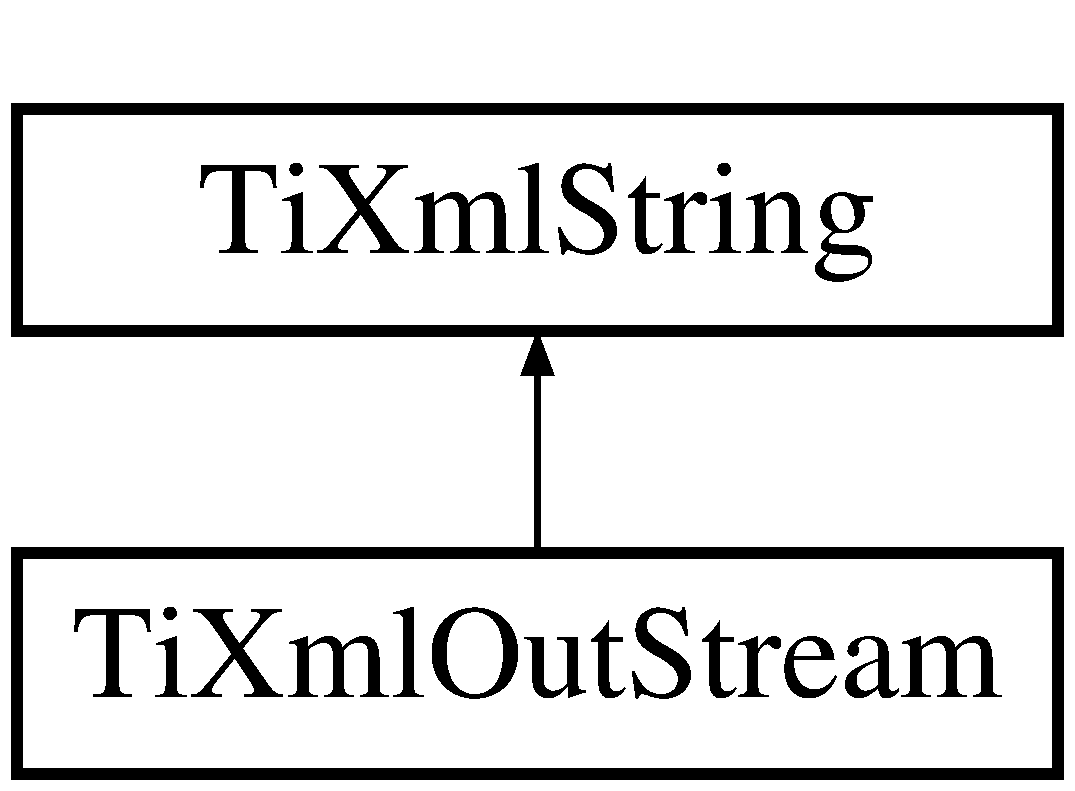
\includegraphics[height=2cm]{classTiXmlOutStream}
\end{center}
\end{figure}
\subsection*{Public Member Functions}
\begin{CompactItemize}
\item 
{\bf TiXmlOutStream} \& {\bf operator$<$$<$} (const {\bf TiXmlString} \&in)
\item 
{\bf TiXmlOutStream} \& {\bf operator$<$$<$} (const char $\ast$in)
\end{CompactItemize}


\subsection{Member Function Documentation}
\index{TiXmlOutStream@{TiXmlOutStream}!operator$<$$<$@{operator$<$$<$}}
\index{operator$<$$<$@{operator$<$$<$}!TiXmlOutStream@{TiXmlOutStream}}
\subsubsection{\setlength{\rightskip}{0pt plus 5cm}{\bf TiXmlOutStream}\& TiXmlOutStream::operator$<$$<$ (const {\bf TiXmlString} \& {\em in})\hspace{0.3cm}{\tt  [inline]}}\label{classTiXmlOutStream_3640dcb1c0903be3bc6966cdc9a79db6}


\index{TiXmlOutStream@{TiXmlOutStream}!operator$<$$<$@{operator$<$$<$}}
\index{operator$<$$<$@{operator$<$$<$}!TiXmlOutStream@{TiXmlOutStream}}
\subsubsection{\setlength{\rightskip}{0pt plus 5cm}{\bf TiXmlOutStream}\& TiXmlOutStream::operator$<$$<$ (const char $\ast$ {\em in})\hspace{0.3cm}{\tt  [inline]}}\label{classTiXmlOutStream_f2117e5a8cbfcb69544804ad2859bfb6}




The documentation for this class was generated from the following file:\begin{CompactItemize}
\item 
/home/msneddon/eclipse/ganymede\_\-cpp/workspace/NFsim\_\-svn/src/NFinput/TinyXML/{\bf tinystr.h}\end{CompactItemize}

\section{TiXmlParsingData Class Reference}
\label{classTiXmlParsingData}\index{TiXmlParsingData@{TiXmlParsingData}}
\subsection*{Public Member Functions}
\begin{CompactItemize}
\item 
void {\bf Stamp} (const char $\ast$now, {\bf TiXmlEncoding} encoding)
\item 
const {\bf TiXmlCursor} \& {\bf Cursor} ()
\end{CompactItemize}
\subsection*{Friends}
\begin{CompactItemize}
\item 
class {\bf TiXmlDocument}
\end{CompactItemize}


\subsection{Member Function Documentation}
\index{TiXmlParsingData@{TiXmlParsingData}!Stamp@{Stamp}}
\index{Stamp@{Stamp}!TiXmlParsingData@{TiXmlParsingData}}
\subsubsection{\setlength{\rightskip}{0pt plus 5cm}void TiXmlParsingData::Stamp (const char $\ast$ {\em now}, {\bf TiXmlEncoding} {\em encoding})}\label{classTiXmlParsingData_65cee8ab77a36c605db08c84b4c30a7d}


\index{TiXmlParsingData@{TiXmlParsingData}!Cursor@{Cursor}}
\index{Cursor@{Cursor}!TiXmlParsingData@{TiXmlParsingData}}
\subsubsection{\setlength{\rightskip}{0pt plus 5cm}const {\bf TiXmlCursor}\& TiXmlParsingData::Cursor ()\hspace{0.3cm}{\tt  [inline]}}\label{classTiXmlParsingData_56908a17d7d7a6b2e511e62cf1d40d05}




\subsection{Friends And Related Function Documentation}
\index{TiXmlParsingData@{TiXmlParsingData}!TiXmlDocument@{TiXmlDocument}}
\index{TiXmlDocument@{TiXmlDocument}!TiXmlParsingData@{TiXmlParsingData}}
\subsubsection{\setlength{\rightskip}{0pt plus 5cm}friend class {\bf TiXmlDocument}\hspace{0.3cm}{\tt  [friend]}}\label{classTiXmlParsingData_173617f6dfe902cf484ce5552b950475}




The documentation for this class was generated from the following file:\begin{CompactItemize}
\item 
/home/msneddon/eclipse/galileoSR1\_\-cpp/workspace/NFsim/src/NFinput/TinyXML/{\bf tinyxmlparser.cpp}\end{CompactItemize}

\section{TiXmlPrinter Class Reference}
\label{classTiXmlPrinter}\index{TiXmlPrinter@{TiXmlPrinter}}
{\tt \#include $<$tinyxml.h$>$}

Inheritance diagram for TiXmlPrinter::\begin{figure}[H]
\begin{center}
\leavevmode
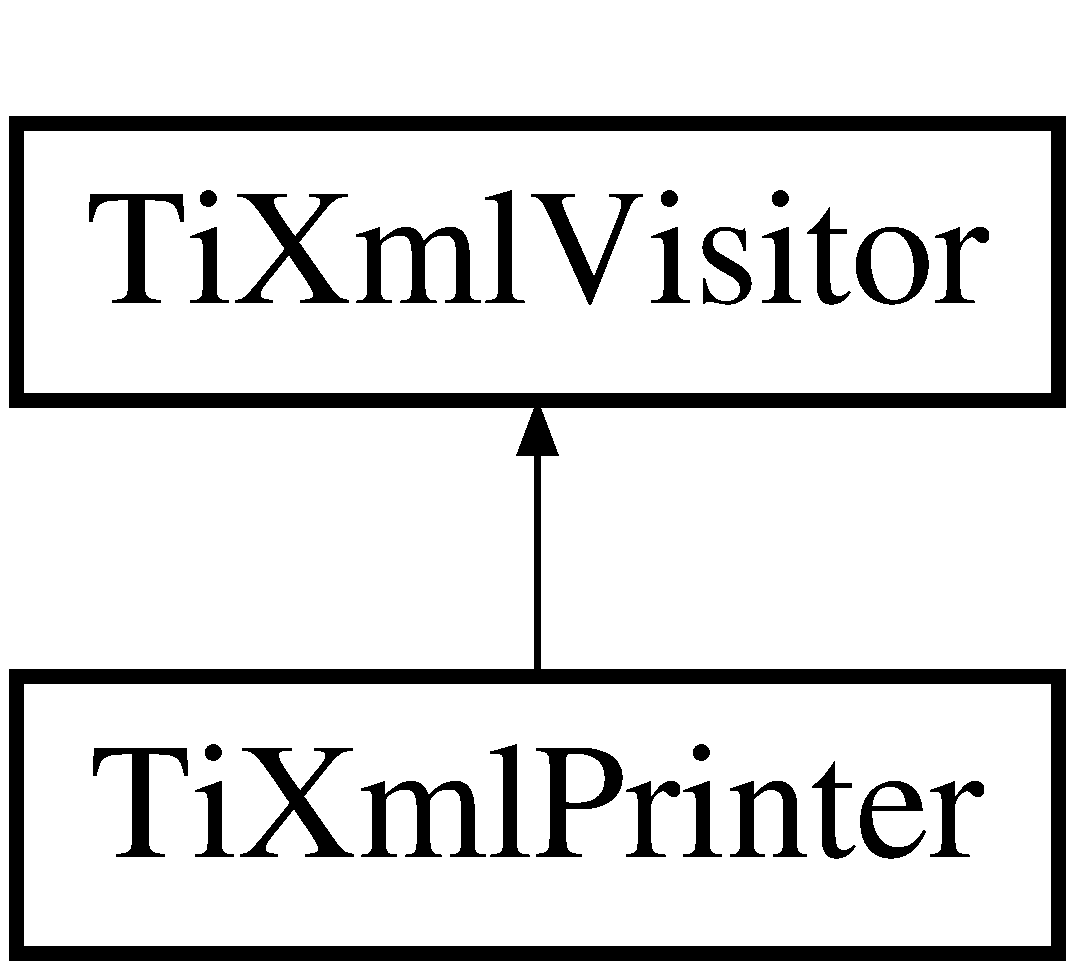
\includegraphics[height=2cm]{classTiXmlPrinter}
\end{center}
\end{figure}


\subsection{Detailed Description}
Print to memory functionality. The \doxyref{TiXmlPrinter}{p.}{classTiXmlPrinter} is useful when you need to:

\begin{enumerate}
\item Print to memory (especially in non-STL mode)\item Control formatting (line endings, etc.)\end{enumerate}


When constructed, the \doxyref{TiXmlPrinter}{p.}{classTiXmlPrinter} is in its default \char`\"{}pretty printing\char`\"{} mode. Before calling Accept() you can call methods to control the printing of the XML document. After \doxyref{TiXmlNode::Accept()}{p.}{classTiXmlNode_cc0f88b7462c6cb73809d410a4f5bb86} is called, the printed document can be accessed via the \doxyref{CStr()}{p.}{classTiXmlPrinter_859eede9597d3e0355b77757be48735e}, Str(), and \doxyref{Size()}{p.}{classTiXmlPrinter_d01375ae9199bd2f48252eaddce3039d} methods.

\doxyref{TiXmlPrinter}{p.}{classTiXmlPrinter} uses the Visitor API. 

\footnotesize\begin{verbatim}
	TiXmlPrinter printer;
	printer.SetIndent( "\t" );

	doc.Accept( &printer );
	fprintf( stdout, "%s", printer.CStr() );
	\end{verbatim}
\normalsize
 \subsection*{Public Member Functions}
\begin{CompactItemize}
\item 
{\bf TiXmlPrinter} ()
\item 
virtual bool {\bf VisitEnter} (const {\bf TiXmlDocument} \&doc)
\begin{CompactList}\small\item\em Visit a document. \item\end{CompactList}\item 
virtual bool {\bf VisitExit} (const {\bf TiXmlDocument} \&doc)
\begin{CompactList}\small\item\em Visit a document. \item\end{CompactList}\item 
virtual bool {\bf VisitEnter} (const {\bf TiXmlElement} \&element, const {\bf TiXmlAttribute} $\ast$firstAttribute)
\begin{CompactList}\small\item\em Visit an element. \item\end{CompactList}\item 
virtual bool {\bf VisitExit} (const {\bf TiXmlElement} \&element)
\begin{CompactList}\small\item\em Visit an element. \item\end{CompactList}\item 
virtual bool {\bf Visit} (const {\bf TiXmlDeclaration} \&declaration)
\begin{CompactList}\small\item\em Visit a declaration. \item\end{CompactList}\item 
virtual bool {\bf Visit} (const {\bf TiXmlText} \&text)
\begin{CompactList}\small\item\em Visit a text node. \item\end{CompactList}\item 
virtual bool {\bf Visit} (const {\bf TiXmlComment} \&comment)
\begin{CompactList}\small\item\em Visit a comment node. \item\end{CompactList}\item 
virtual bool {\bf Visit} (const {\bf TiXmlUnknown} \&unknown)
\begin{CompactList}\small\item\em Visit an unknow node. \item\end{CompactList}\item 
void {\bf SetIndent} (const char $\ast$\_\-indent)
\item 
const char $\ast$ {\bf Indent} ()
\begin{CompactList}\small\item\em Query the indention string. \item\end{CompactList}\item 
void {\bf SetLineBreak} (const char $\ast$\_\-lineBreak)
\item 
const char $\ast$ {\bf LineBreak} ()
\begin{CompactList}\small\item\em Query the current line breaking string. \item\end{CompactList}\item 
void {\bf SetStreamPrinting} ()
\item 
const char $\ast$ {\bf CStr} ()
\begin{CompactList}\small\item\em Return the result. \item\end{CompactList}\item 
size\_\-t {\bf Size} ()
\begin{CompactList}\small\item\em Return the length of the result string. \item\end{CompactList}\end{CompactItemize}


\subsection{Constructor \& Destructor Documentation}
\index{TiXmlPrinter@{TiXmlPrinter}!TiXmlPrinter@{TiXmlPrinter}}
\index{TiXmlPrinter@{TiXmlPrinter}!TiXmlPrinter@{TiXmlPrinter}}
\subsubsection{\setlength{\rightskip}{0pt plus 5cm}TiXmlPrinter::TiXmlPrinter ()\hspace{0.3cm}{\tt  [inline]}}\label{classTiXmlPrinter_6539b864026c8667cd0bd5fdf4b41f43}




\subsection{Member Function Documentation}
\index{TiXmlPrinter@{TiXmlPrinter}!VisitEnter@{VisitEnter}}
\index{VisitEnter@{VisitEnter}!TiXmlPrinter@{TiXmlPrinter}}
\subsubsection{\setlength{\rightskip}{0pt plus 5cm}bool TiXmlPrinter::VisitEnter (const {\bf TiXmlDocument} \&)\hspace{0.3cm}{\tt  [virtual]}}\label{classTiXmlPrinter_2ec73087db26ff4d2c4316c56f861db7}


Visit a document. 



Reimplemented from {\bf TiXmlVisitor} \doxyref{}{p.}{classTiXmlVisitor_07baecb52dd7d8716ae2a48ad0956ee0}.\index{TiXmlPrinter@{TiXmlPrinter}!VisitExit@{VisitExit}}
\index{VisitExit@{VisitExit}!TiXmlPrinter@{TiXmlPrinter}}
\subsubsection{\setlength{\rightskip}{0pt plus 5cm}bool TiXmlPrinter::VisitExit (const {\bf TiXmlDocument} \&)\hspace{0.3cm}{\tt  [virtual]}}\label{classTiXmlPrinter_0a636046fa589b6d7f3e5bd025b3f33e}


Visit a document. 



Reimplemented from {\bf TiXmlVisitor} \doxyref{}{p.}{classTiXmlVisitor_a0ade4f27087447e93974e975c3246ad}.\index{TiXmlPrinter@{TiXmlPrinter}!VisitEnter@{VisitEnter}}
\index{VisitEnter@{VisitEnter}!TiXmlPrinter@{TiXmlPrinter}}
\subsubsection{\setlength{\rightskip}{0pt plus 5cm}bool TiXmlPrinter::VisitEnter (const {\bf TiXmlElement} \&, const {\bf TiXmlAttribute} $\ast$)\hspace{0.3cm}{\tt  [virtual]}}\label{classTiXmlPrinter_6dccaf5ee4979f13877690afe28721e8}


Visit an element. 



Reimplemented from {\bf TiXmlVisitor} \doxyref{}{p.}{classTiXmlVisitor_f6c6178ffa517bbdba95d70490875fff}.\index{TiXmlPrinter@{TiXmlPrinter}!VisitExit@{VisitExit}}
\index{VisitExit@{VisitExit}!TiXmlPrinter@{TiXmlPrinter}}
\subsubsection{\setlength{\rightskip}{0pt plus 5cm}bool TiXmlPrinter::VisitExit (const {\bf TiXmlElement} \&)\hspace{0.3cm}{\tt  [virtual]}}\label{classTiXmlPrinter_e6a1df8271df4bf62d7873c38e34aa69}


Visit an element. 



Reimplemented from {\bf TiXmlVisitor} \doxyref{}{p.}{classTiXmlVisitor_ec2b1f8116226d52f3a1b95dafd3a32c}.\index{TiXmlPrinter@{TiXmlPrinter}!Visit@{Visit}}
\index{Visit@{Visit}!TiXmlPrinter@{TiXmlPrinter}}
\subsubsection{\setlength{\rightskip}{0pt plus 5cm}bool TiXmlPrinter::Visit (const {\bf TiXmlDeclaration} \&)\hspace{0.3cm}{\tt  [virtual]}}\label{classTiXmlPrinter_daf7eec4dc43ad071ff52b60361574f5}


Visit a declaration. 



Reimplemented from {\bf TiXmlVisitor} \doxyref{}{p.}{classTiXmlVisitor_fad71c71ce6473fb9b4b64cd92de4a19}.\index{TiXmlPrinter@{TiXmlPrinter}!Visit@{Visit}}
\index{Visit@{Visit}!TiXmlPrinter@{TiXmlPrinter}}
\subsubsection{\setlength{\rightskip}{0pt plus 5cm}bool TiXmlPrinter::Visit (const {\bf TiXmlText} \&)\hspace{0.3cm}{\tt  [virtual]}}\label{classTiXmlPrinter_0857c5d32c59b9a257f9a49cb9411df5}


Visit a text node. 



Reimplemented from {\bf TiXmlVisitor} \doxyref{}{p.}{classTiXmlVisitor_399b8ebca5cd14664974a32d2ce029e5}.\index{TiXmlPrinter@{TiXmlPrinter}!Visit@{Visit}}
\index{Visit@{Visit}!TiXmlPrinter@{TiXmlPrinter}}
\subsubsection{\setlength{\rightskip}{0pt plus 5cm}bool TiXmlPrinter::Visit (const {\bf TiXmlComment} \&)\hspace{0.3cm}{\tt  [virtual]}}\label{classTiXmlPrinter_9870423f5603630e6142f6bdb66dfb57}


Visit a comment node. 



Reimplemented from {\bf TiXmlVisitor} \doxyref{}{p.}{classTiXmlVisitor_53a60e7a528627b31af3161972cc7fa2}.\index{TiXmlPrinter@{TiXmlPrinter}!Visit@{Visit}}
\index{Visit@{Visit}!TiXmlPrinter@{TiXmlPrinter}}
\subsubsection{\setlength{\rightskip}{0pt plus 5cm}bool TiXmlPrinter::Visit (const {\bf TiXmlUnknown} \&)\hspace{0.3cm}{\tt  [virtual]}}\label{classTiXmlPrinter_08591a15c9a07afa83c24e08b03d6358}


Visit an unknow node. 



Reimplemented from {\bf TiXmlVisitor} \doxyref{}{p.}{classTiXmlVisitor_7e284d607d275c51dac1adb58159ce28}.\index{TiXmlPrinter@{TiXmlPrinter}!SetIndent@{SetIndent}}
\index{SetIndent@{SetIndent}!TiXmlPrinter@{TiXmlPrinter}}
\subsubsection{\setlength{\rightskip}{0pt plus 5cm}void TiXmlPrinter::SetIndent (const char $\ast$ {\em \_\-indent})\hspace{0.3cm}{\tt  [inline]}}\label{classTiXmlPrinter_213377a4070c7e625bae59716b089e5e}


Set the indent characters for printing. By default 4 spaces but tab ($\backslash$t) is also useful, or null/empty string for no indentation. \index{TiXmlPrinter@{TiXmlPrinter}!Indent@{Indent}}
\index{Indent@{Indent}!TiXmlPrinter@{TiXmlPrinter}}
\subsubsection{\setlength{\rightskip}{0pt plus 5cm}const char$\ast$ TiXmlPrinter::Indent ()\hspace{0.3cm}{\tt  [inline]}}\label{classTiXmlPrinter_bb33ec7d4bad6aaeb57f4304394b133d}


Query the indention string. 

\index{TiXmlPrinter@{TiXmlPrinter}!SetLineBreak@{SetLineBreak}}
\index{SetLineBreak@{SetLineBreak}!TiXmlPrinter@{TiXmlPrinter}}
\subsubsection{\setlength{\rightskip}{0pt plus 5cm}void TiXmlPrinter::SetLineBreak (const char $\ast$ {\em \_\-lineBreak})\hspace{0.3cm}{\tt  [inline]}}\label{classTiXmlPrinter_4be1e37e69e3858c59635aa947174fe6}


Set the line breaking string. By default set to newline (\par
). Some operating systems prefer other characters, or can be set to the null/empty string for no indenation. \index{TiXmlPrinter@{TiXmlPrinter}!LineBreak@{LineBreak}}
\index{LineBreak@{LineBreak}!TiXmlPrinter@{TiXmlPrinter}}
\subsubsection{\setlength{\rightskip}{0pt plus 5cm}const char$\ast$ TiXmlPrinter::LineBreak ()\hspace{0.3cm}{\tt  [inline]}}\label{classTiXmlPrinter_11f1b4804a460b175ec244eb5724d96d}


Query the current line breaking string. 

\index{TiXmlPrinter@{TiXmlPrinter}!SetStreamPrinting@{SetStreamPrinting}}
\index{SetStreamPrinting@{SetStreamPrinting}!TiXmlPrinter@{TiXmlPrinter}}
\subsubsection{\setlength{\rightskip}{0pt plus 5cm}void TiXmlPrinter::SetStreamPrinting ()\hspace{0.3cm}{\tt  [inline]}}\label{classTiXmlPrinter_b23a90629e374cb1cadca090468bbd19}


Switch over to \char`\"{}stream printing\char`\"{} which is the most dense formatting without linebreaks. Common when the XML is needed for network transmission. \index{TiXmlPrinter@{TiXmlPrinter}!CStr@{CStr}}
\index{CStr@{CStr}!TiXmlPrinter@{TiXmlPrinter}}
\subsubsection{\setlength{\rightskip}{0pt plus 5cm}const char$\ast$ TiXmlPrinter::CStr ()\hspace{0.3cm}{\tt  [inline]}}\label{classTiXmlPrinter_859eede9597d3e0355b77757be48735e}


Return the result. 

\index{TiXmlPrinter@{TiXmlPrinter}!Size@{Size}}
\index{Size@{Size}!TiXmlPrinter@{TiXmlPrinter}}
\subsubsection{\setlength{\rightskip}{0pt plus 5cm}size\_\-t TiXmlPrinter::Size ()\hspace{0.3cm}{\tt  [inline]}}\label{classTiXmlPrinter_d01375ae9199bd2f48252eaddce3039d}


Return the length of the result string. 



The documentation for this class was generated from the following files:\begin{CompactItemize}
\item 
/home/msneddon/eclipse/ganymede\_\-cpp/workspace/NFsim\_\-svn/src/NFinput/TinyXML/{\bf tinyxml.h}\item 
/home/msneddon/eclipse/ganymede\_\-cpp/workspace/NFsim\_\-svn/src/NFinput/TinyXML/{\bf tinyxml.cpp}\end{CompactItemize}

\section{TiXmlString Class Reference}
\label{classTiXmlString}\index{TiXmlString@{TiXmlString}}
{\tt \#include $<$tinystr.h$>$}

Inheritance diagram for TiXmlString::\begin{figure}[H]
\begin{center}
\leavevmode
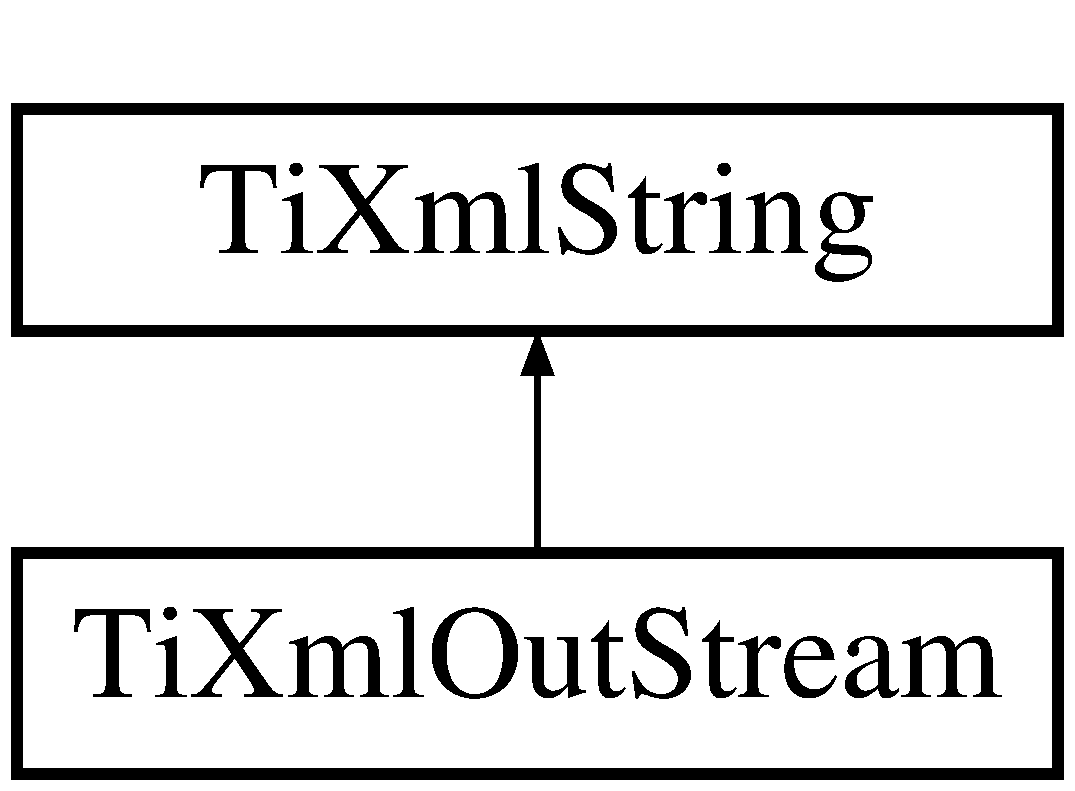
\includegraphics[height=2cm]{classTiXmlString}
\end{center}
\end{figure}
\subsection*{Public Types}
\begin{CompactItemize}
\item 
typedef size\_\-t {\bf size\_\-type}
\end{CompactItemize}
\subsection*{Public Member Functions}
\begin{CompactItemize}
\item 
{\bf TiXmlString} ()
\item 
{\bf TiXmlString} (const {\bf TiXmlString} \&copy)
\item 
TIXML\_\-EXPLICIT {\bf TiXmlString} (const char $\ast$copy)
\item 
TIXML\_\-EXPLICIT {\bf TiXmlString} (const char $\ast$str, {\bf size\_\-type} len)
\item 
{\bf $\sim$TiXmlString} ()
\item 
{\bf TiXmlString} \& {\bf operator=} (const char $\ast$copy)
\item 
{\bf TiXmlString} \& {\bf operator=} (const {\bf TiXmlString} \&copy)
\item 
{\bf TiXmlString} \& {\bf operator+=} (const char $\ast$suffix)
\item 
{\bf TiXmlString} \& {\bf operator+=} (char single)
\item 
{\bf TiXmlString} \& {\bf operator+=} (const {\bf TiXmlString} \&suffix)
\item 
const char $\ast$ {\bf c\_\-str} () const 
\item 
const char $\ast$ {\bf data} () const 
\item 
{\bf size\_\-type} {\bf length} () const 
\item 
{\bf size\_\-type} {\bf size} () const 
\item 
bool {\bf empty} () const 
\item 
{\bf size\_\-type} {\bf capacity} () const 
\item 
const char \& {\bf at} ({\bf size\_\-type} index) const 
\item 
char \& {\bf operator[$\,$]} ({\bf size\_\-type} index) const 
\item 
{\bf size\_\-type} {\bf find} (char lookup) const 
\item 
{\bf size\_\-type} {\bf find} (char tofind, {\bf size\_\-type} offset) const 
\item 
void {\bf clear} ()
\item 
void {\bf reserve} ({\bf size\_\-type} cap)
\item 
{\bf TiXmlString} \& {\bf assign} (const char $\ast$str, {\bf size\_\-type} len)
\item 
{\bf TiXmlString} \& {\bf append} (const char $\ast$str, {\bf size\_\-type} len)
\item 
void {\bf swap} ({\bf TiXmlString} \&other)
\end{CompactItemize}
\subsection*{Static Public Attributes}
\begin{CompactItemize}
\item 
static const {\bf size\_\-type} {\bf npos} = static\_\-cast$<$ {\bf TiXmlString::size\_\-type} $>$(-1)
\end{CompactItemize}
\subsection*{Classes}
\begin{CompactItemize}
\item 
struct \textbf{Rep}
\end{CompactItemize}


\subsection{Member Typedef Documentation}
\index{TiXmlString@{TiXmlString}!size\_\-type@{size\_\-type}}
\index{size\_\-type@{size\_\-type}!TiXmlString@{TiXmlString}}
\subsubsection{\setlength{\rightskip}{0pt plus 5cm}typedef size\_\-t {\bf TiXmlString::size\_\-type}}\label{classTiXmlString_beb2c1893a04c17904f7c06546d0b971}




\subsection{Constructor \& Destructor Documentation}
\index{TiXmlString@{TiXmlString}!TiXmlString@{TiXmlString}}
\index{TiXmlString@{TiXmlString}!TiXmlString@{TiXmlString}}
\subsubsection{\setlength{\rightskip}{0pt plus 5cm}TiXmlString::TiXmlString ()\hspace{0.3cm}{\tt  [inline]}}\label{classTiXmlString_342f61e0fc2244df300b73aedf6d3fef}


\index{TiXmlString@{TiXmlString}!TiXmlString@{TiXmlString}}
\index{TiXmlString@{TiXmlString}!TiXmlString@{TiXmlString}}
\subsubsection{\setlength{\rightskip}{0pt plus 5cm}TiXmlString::TiXmlString (const {\bf TiXmlString} \& {\em copy})\hspace{0.3cm}{\tt  [inline]}}\label{classTiXmlString_c80fe17693a438c9ab2591664743fcb6}


\index{TiXmlString@{TiXmlString}!TiXmlString@{TiXmlString}}
\index{TiXmlString@{TiXmlString}!TiXmlString@{TiXmlString}}
\subsubsection{\setlength{\rightskip}{0pt plus 5cm}TIXML\_\-EXPLICIT TiXmlString::TiXmlString (const char $\ast$ {\em copy})\hspace{0.3cm}{\tt  [inline]}}\label{classTiXmlString_a3b32bd2891a757c9f36c21db44c81d2}


\index{TiXmlString@{TiXmlString}!TiXmlString@{TiXmlString}}
\index{TiXmlString@{TiXmlString}!TiXmlString@{TiXmlString}}
\subsubsection{\setlength{\rightskip}{0pt plus 5cm}TIXML\_\-EXPLICIT TiXmlString::TiXmlString (const char $\ast$ {\em str}, {\bf size\_\-type} {\em len})\hspace{0.3cm}{\tt  [inline]}}\label{classTiXmlString_4b17ea5c5db986f14827223dfa8f1547}


\index{TiXmlString@{TiXmlString}!$\sim$TiXmlString@{$\sim$TiXmlString}}
\index{$\sim$TiXmlString@{$\sim$TiXmlString}!TiXmlString@{TiXmlString}}
\subsubsection{\setlength{\rightskip}{0pt plus 5cm}TiXmlString::$\sim$TiXmlString ()\hspace{0.3cm}{\tt  [inline]}}\label{classTiXmlString_7ac03f581ca3422c4808162ab14f3450}




\subsection{Member Function Documentation}
\index{TiXmlString@{TiXmlString}!operator=@{operator=}}
\index{operator=@{operator=}!TiXmlString@{TiXmlString}}
\subsubsection{\setlength{\rightskip}{0pt plus 5cm}{\bf TiXmlString}\& TiXmlString::operator= (const char $\ast$ {\em copy})\hspace{0.3cm}{\tt  [inline]}}\label{classTiXmlString_e0bc6147afc0ec2aa0da3a3c0a8fcfb0}


\index{TiXmlString@{TiXmlString}!operator=@{operator=}}
\index{operator=@{operator=}!TiXmlString@{TiXmlString}}
\subsubsection{\setlength{\rightskip}{0pt plus 5cm}{\bf TiXmlString}\& TiXmlString::operator= (const {\bf TiXmlString} \& {\em copy})\hspace{0.3cm}{\tt  [inline]}}\label{classTiXmlString_b1f1f5d3eceaa0f22d0a7e6055ea81b0}


\index{TiXmlString@{TiXmlString}!operator+=@{operator+=}}
\index{operator+=@{operator+=}!TiXmlString@{TiXmlString}}
\subsubsection{\setlength{\rightskip}{0pt plus 5cm}{\bf TiXmlString}\& TiXmlString::operator+= (const char $\ast$ {\em suffix})\hspace{0.3cm}{\tt  [inline]}}\label{classTiXmlString_b56336ac2aa2a08d24a71eb9a2b502a5}


\index{TiXmlString@{TiXmlString}!operator+=@{operator+=}}
\index{operator+=@{operator+=}!TiXmlString@{TiXmlString}}
\subsubsection{\setlength{\rightskip}{0pt plus 5cm}{\bf TiXmlString}\& TiXmlString::operator+= (char {\em single})\hspace{0.3cm}{\tt  [inline]}}\label{classTiXmlString_6aa09d5240470b76d54ec709e04f8c13}


\index{TiXmlString@{TiXmlString}!operator+=@{operator+=}}
\index{operator+=@{operator+=}!TiXmlString@{TiXmlString}}
\subsubsection{\setlength{\rightskip}{0pt plus 5cm}{\bf TiXmlString}\& TiXmlString::operator+= (const {\bf TiXmlString} \& {\em suffix})\hspace{0.3cm}{\tt  [inline]}}\label{classTiXmlString_fdcae5ea2b4d9e194dc21226b817f417}


\index{TiXmlString@{TiXmlString}!c\_\-str@{c\_\-str}}
\index{c\_\-str@{c\_\-str}!TiXmlString@{TiXmlString}}
\subsubsection{\setlength{\rightskip}{0pt plus 5cm}const char$\ast$ TiXmlString::c\_\-str () const\hspace{0.3cm}{\tt  [inline]}}\label{classTiXmlString_5581ca641d915551d3cda90f8e7bf49b}


\index{TiXmlString@{TiXmlString}!data@{data}}
\index{data@{data}!TiXmlString@{TiXmlString}}
\subsubsection{\setlength{\rightskip}{0pt plus 5cm}const char$\ast$ TiXmlString::data () const\hspace{0.3cm}{\tt  [inline]}}\label{classTiXmlString_00abc60f135c7ca1951c7334cc2c7993}


\index{TiXmlString@{TiXmlString}!length@{length}}
\index{length@{length}!TiXmlString@{TiXmlString}}
\subsubsection{\setlength{\rightskip}{0pt plus 5cm}{\bf size\_\-type} TiXmlString::length () const\hspace{0.3cm}{\tt  [inline]}}\label{classTiXmlString_3202f27d139a3fac79205f1f3c707727}


\index{TiXmlString@{TiXmlString}!size@{size}}
\index{size@{size}!TiXmlString@{TiXmlString}}
\subsubsection{\setlength{\rightskip}{0pt plus 5cm}{\bf size\_\-type} TiXmlString::size () const\hspace{0.3cm}{\tt  [inline]}}\label{classTiXmlString_96103e5c0f67e987fa48527e1f47a1f6}


\index{TiXmlString@{TiXmlString}!empty@{empty}}
\index{empty@{empty}!TiXmlString@{TiXmlString}}
\subsubsection{\setlength{\rightskip}{0pt plus 5cm}bool TiXmlString::empty () const\hspace{0.3cm}{\tt  [inline]}}\label{classTiXmlString_9a61e1d11cdb71bea4a4ed79caa793f4}


\index{TiXmlString@{TiXmlString}!capacity@{capacity}}
\index{capacity@{capacity}!TiXmlString@{TiXmlString}}
\subsubsection{\setlength{\rightskip}{0pt plus 5cm}{\bf size\_\-type} TiXmlString::capacity () const\hspace{0.3cm}{\tt  [inline]}}\label{classTiXmlString_76e4d6aba7845f4cf9c02332a5fbf916}


\index{TiXmlString@{TiXmlString}!at@{at}}
\index{at@{at}!TiXmlString@{TiXmlString}}
\subsubsection{\setlength{\rightskip}{0pt plus 5cm}const char\& TiXmlString::at ({\bf size\_\-type} {\em index}) const\hspace{0.3cm}{\tt  [inline]}}\label{classTiXmlString_6763093267bbdecbf03f8840bc349877}


\index{TiXmlString@{TiXmlString}!operator[]@{operator[]}}
\index{operator[]@{operator[]}!TiXmlString@{TiXmlString}}
\subsubsection{\setlength{\rightskip}{0pt plus 5cm}char\& TiXmlString::operator[$\,$] ({\bf size\_\-type} {\em index}) const\hspace{0.3cm}{\tt  [inline]}}\label{classTiXmlString_e8cdc1d46c538536b786f7ae03c0c1d9}


\index{TiXmlString@{TiXmlString}!find@{find}}
\index{find@{find}!TiXmlString@{TiXmlString}}
\subsubsection{\setlength{\rightskip}{0pt plus 5cm}{\bf size\_\-type} TiXmlString::find (char {\em lookup}) const\hspace{0.3cm}{\tt  [inline]}}\label{classTiXmlString_5c2b368b5eafe075fd9565cbcbd4c2f9}


\index{TiXmlString@{TiXmlString}!find@{find}}
\index{find@{find}!TiXmlString@{TiXmlString}}
\subsubsection{\setlength{\rightskip}{0pt plus 5cm}{\bf size\_\-type} TiXmlString::find (char {\em tofind}, {\bf size\_\-type} {\em offset}) const\hspace{0.3cm}{\tt  [inline]}}\label{classTiXmlString_5f2a6fd565751410b392f249a9786db4}


\index{TiXmlString@{TiXmlString}!clear@{clear}}
\index{clear@{clear}!TiXmlString@{TiXmlString}}
\subsubsection{\setlength{\rightskip}{0pt plus 5cm}void TiXmlString::clear ()\hspace{0.3cm}{\tt  [inline]}}\label{classTiXmlString_b20e06e4c666abf3bdbfb3a1191d4888}


\index{TiXmlString@{TiXmlString}!reserve@{reserve}}
\index{reserve@{reserve}!TiXmlString@{TiXmlString}}
\subsubsection{\setlength{\rightskip}{0pt plus 5cm}void TiXmlString::reserve ({\bf size\_\-type} {\em cap})}\label{classTiXmlString_88ecf9f0f00cb5c67b6b637958d7049c}


\index{TiXmlString@{TiXmlString}!assign@{assign}}
\index{assign@{assign}!TiXmlString@{TiXmlString}}
\subsubsection{\setlength{\rightskip}{0pt plus 5cm}{\bf TiXmlString} \& TiXmlString::assign (const char $\ast$ {\em str}, {\bf size\_\-type} {\em len})}\label{classTiXmlString_c72f3d9149b7812c1e6c59402014d0d5}


\index{TiXmlString@{TiXmlString}!append@{append}}
\index{append@{append}!TiXmlString@{TiXmlString}}
\subsubsection{\setlength{\rightskip}{0pt plus 5cm}{\bf TiXmlString} \& TiXmlString::append (const char $\ast$ {\em str}, {\bf size\_\-type} {\em len})}\label{classTiXmlString_d44b21700d2ec24a511367b222b643fb}


\index{TiXmlString@{TiXmlString}!swap@{swap}}
\index{swap@{swap}!TiXmlString@{TiXmlString}}
\subsubsection{\setlength{\rightskip}{0pt plus 5cm}void TiXmlString::swap ({\bf TiXmlString} \& {\em other})\hspace{0.3cm}{\tt  [inline]}}\label{classTiXmlString_a392cbc180752a79f007f4f9280c7762}




\subsection{Member Data Documentation}
\index{TiXmlString@{TiXmlString}!npos@{npos}}
\index{npos@{npos}!TiXmlString@{TiXmlString}}
\subsubsection{\setlength{\rightskip}{0pt plus 5cm}const {\bf TiXmlString::size\_\-type} {\bf TiXmlString::npos} = static\_\-cast$<$ {\bf TiXmlString::size\_\-type} $>$(-1)\hspace{0.3cm}{\tt  [static]}}\label{classTiXmlString_8f4422d227088dc7bec96f479b275d0a}




The documentation for this class was generated from the following files:\begin{CompactItemize}
\item 
/home/msneddon/eclipse/indigo/workspace/NFsim/src/NFinput/TinyXML/{\bf tinystr.h}\item 
/home/msneddon/eclipse/indigo/workspace/NFsim/src/NFinput/TinyXML/{\bf tinystr.cpp}\end{CompactItemize}

\section{TiXmlText Class Reference}
\label{classTiXmlText}\index{TiXmlText@{TiXmlText}}
{\tt \#include $<$tinyxml.h$>$}

Inheritance diagram for TiXmlText::\begin{figure}[H]
\begin{center}
\leavevmode
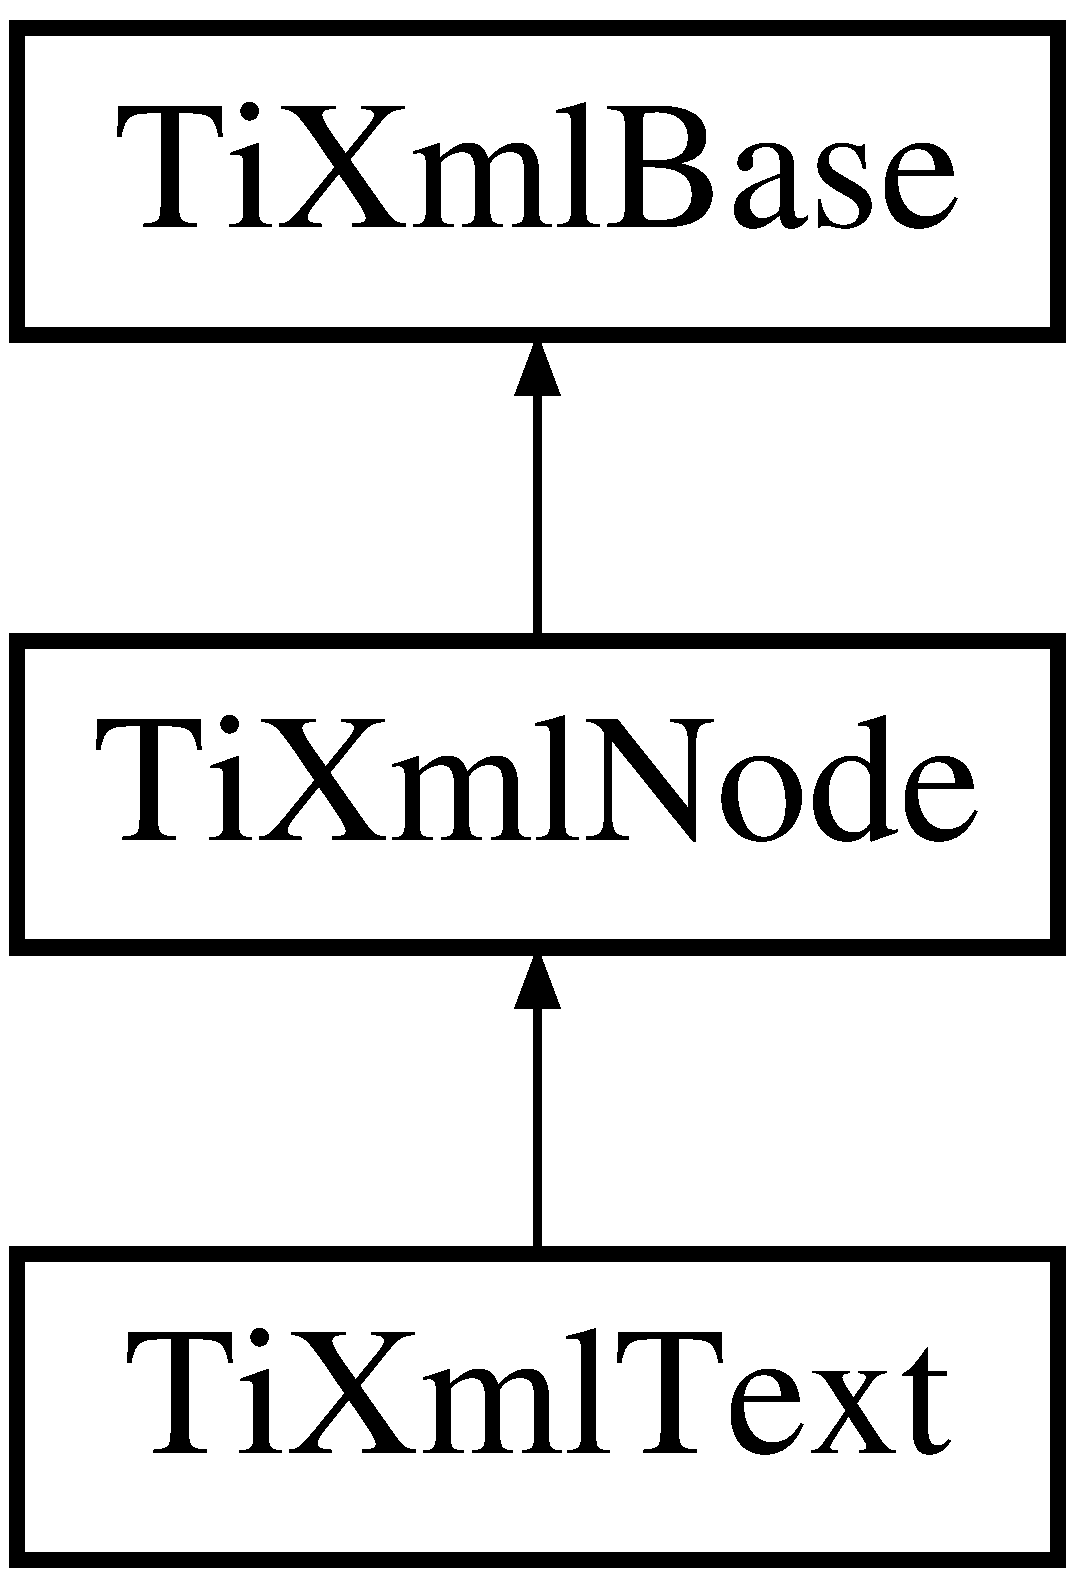
\includegraphics[height=3cm]{classTiXmlText}
\end{center}
\end{figure}


\subsection{Detailed Description}
XML text. A text node can have 2 ways to output the next. \char`\"{}normal\char`\"{} output and CDATA. It will default to the mode it was parsed from the XML file and you generally want to leave it alone, but you can change the output mode with \doxyref{SetCDATA()}{p.}{classTiXmlText_cb17ff7c5d09b2c839393445a3de5ea9} and query it with \doxyref{CDATA()}{p.}{classTiXmlText_d1a6a6b83fa2271022dd97c072a2b586}. \subsection*{Public Member Functions}
\begin{CompactItemize}
\item 
{\bf TiXmlText} (const char $\ast$initValue)
\item 
virtual {\bf $\sim$TiXmlText} ()
\item 
{\bf TiXmlText} (const {\bf TiXmlText} \&copy)
\item 
void {\bf operator=} (const {\bf TiXmlText} \&base)
\item 
virtual void {\bf Print} (FILE $\ast$cfile, int depth) const 
\item 
bool {\bf CDATA} () const 
\begin{CompactList}\small\item\em Queries whether this represents text using a CDATA section. \item\end{CompactList}\item 
void {\bf SetCDATA} (bool \_\-cdata)
\begin{CompactList}\small\item\em Turns on or off a CDATA representation of text. \item\end{CompactList}\item 
virtual const char $\ast$ {\bf Parse} (const char $\ast$p, {\bf TiXmlParsingData} $\ast$data, {\bf TiXmlEncoding} encoding)
\item 
virtual const {\bf TiXmlText} $\ast$ {\bf ToText} () const 
\begin{CompactList}\small\item\em Cast to a more defined type. Will return null not of the requested type. \item\end{CompactList}\item 
virtual {\bf TiXmlText} $\ast$ {\bf ToText} ()
\begin{CompactList}\small\item\em Cast to a more defined type. Will return null not of the requested type. \item\end{CompactList}\item 
virtual bool {\bf Accept} ({\bf TiXmlVisitor} $\ast$content) const 
\end{CompactItemize}
\subsection*{Protected Member Functions}
\begin{CompactItemize}
\item 
virtual {\bf TiXmlNode} $\ast$ {\bf Clone} () const 
\begin{CompactList}\small\item\em [internal use] Creates a new Element and returns it. \item\end{CompactList}\item 
void {\bf CopyTo} ({\bf TiXmlText} $\ast$target) const 
\item 
bool {\bf Blank} () const 
\end{CompactItemize}
\subsection*{Friends}
\begin{CompactItemize}
\item 
class {\bf TiXmlElement}
\end{CompactItemize}


\subsection{Constructor \& Destructor Documentation}
\index{TiXmlText@{TiXmlText}!TiXmlText@{TiXmlText}}
\index{TiXmlText@{TiXmlText}!TiXmlText@{TiXmlText}}
\subsubsection{\setlength{\rightskip}{0pt plus 5cm}TiXmlText::TiXmlText (const char $\ast$ {\em initValue})\hspace{0.3cm}{\tt  [inline]}}\label{classTiXmlText_f659e77c6b87d684827f35a8f4895960}


Constructor for text element. By default, it is treated as normal, encoded text. If you want it be output as a CDATA text element, set the parameter \_\-cdata to 'true' \index{TiXmlText@{TiXmlText}!$\sim$TiXmlText@{$\sim$TiXmlText}}
\index{$\sim$TiXmlText@{$\sim$TiXmlText}!TiXmlText@{TiXmlText}}
\subsubsection{\setlength{\rightskip}{0pt plus 5cm}virtual TiXmlText::$\sim$TiXmlText ()\hspace{0.3cm}{\tt  [inline, virtual]}}\label{classTiXmlText_829a4bd2d8d2461c333eb4f3f5b1b3d2}


\index{TiXmlText@{TiXmlText}!TiXmlText@{TiXmlText}}
\index{TiXmlText@{TiXmlText}!TiXmlText@{TiXmlText}}
\subsubsection{\setlength{\rightskip}{0pt plus 5cm}TiXmlText::TiXmlText (const {\bf TiXmlText} \& {\em copy})\hspace{0.3cm}{\tt  [inline]}}\label{classTiXmlText_8d2cc1b4af2208cbb0171cf20f6815d1}




\subsection{Member Function Documentation}
\index{TiXmlText@{TiXmlText}!operator=@{operator=}}
\index{operator=@{operator=}!TiXmlText@{TiXmlText}}
\subsubsection{\setlength{\rightskip}{0pt plus 5cm}void TiXmlText::operator= (const {\bf TiXmlText} \& {\em base})\hspace{0.3cm}{\tt  [inline]}}\label{classTiXmlText_f5f15d40d048cea7cab9d0eb4fd8a7d2}


\index{TiXmlText@{TiXmlText}!Print@{Print}}
\index{Print@{Print}!TiXmlText@{TiXmlText}}
\subsubsection{\setlength{\rightskip}{0pt plus 5cm}void TiXmlText::Print (FILE $\ast$ {\em cfile}, int {\em depth}) const\hspace{0.3cm}{\tt  [virtual]}}\label{classTiXmlText_e74d56c5b3ddec6cc3103dd51821af92}


All TinyXml classes can print themselves to a filestream or the string class (\doxyref{TiXmlString}{p.}{classTiXmlString} in non-STL mode, std::string in STL mode.) Either or both cfile and str can be null.

This is a formatted print, and will insert tabs and newlines.

(For an unformatted stream, use the $<$$<$ operator.) 

Implements {\bf TiXmlBase} \doxyref{}{p.}{classTiXmlBase_0de56b3f2ef14c65091a3b916437b512}.\index{TiXmlText@{TiXmlText}!CDATA@{CDATA}}
\index{CDATA@{CDATA}!TiXmlText@{TiXmlText}}
\subsubsection{\setlength{\rightskip}{0pt plus 5cm}bool TiXmlText::CDATA () const\hspace{0.3cm}{\tt  [inline]}}\label{classTiXmlText_d1a6a6b83fa2271022dd97c072a2b586}


Queries whether this represents text using a CDATA section. 

\index{TiXmlText@{TiXmlText}!SetCDATA@{SetCDATA}}
\index{SetCDATA@{SetCDATA}!TiXmlText@{TiXmlText}}
\subsubsection{\setlength{\rightskip}{0pt plus 5cm}void TiXmlText::SetCDATA (bool {\em \_\-cdata})\hspace{0.3cm}{\tt  [inline]}}\label{classTiXmlText_cb17ff7c5d09b2c839393445a3de5ea9}


Turns on or off a CDATA representation of text. 

\index{TiXmlText@{TiXmlText}!Parse@{Parse}}
\index{Parse@{Parse}!TiXmlText@{TiXmlText}}
\subsubsection{\setlength{\rightskip}{0pt plus 5cm}const char $\ast$ TiXmlText::Parse (const char $\ast$ {\em p}, {\bf TiXmlParsingData} $\ast$ {\em data}, {\bf TiXmlEncoding} {\em encoding})\hspace{0.3cm}{\tt  [virtual]}}\label{classTiXmlText_8d2dcfa41fc73d3e62dacc2fcf633819}




Implements {\bf TiXmlBase} \doxyref{}{p.}{classTiXmlBase_00e4edb0219d00a1379c856e5a1d2025}.\index{TiXmlText@{TiXmlText}!ToText@{ToText}}
\index{ToText@{ToText}!TiXmlText@{TiXmlText}}
\subsubsection{\setlength{\rightskip}{0pt plus 5cm}virtual const {\bf TiXmlText}$\ast$ TiXmlText::ToText () const\hspace{0.3cm}{\tt  [inline, virtual]}}\label{classTiXmlText_895bf34ffad17f7439ab2a52b9651648}


Cast to a more defined type. Will return null not of the requested type. 



Reimplemented from {\bf TiXmlNode} \doxyref{}{p.}{classTiXmlNode_95a46a52c525992d6b4ee08beb14cd69}.\index{TiXmlText@{TiXmlText}!ToText@{ToText}}
\index{ToText@{ToText}!TiXmlText@{TiXmlText}}
\subsubsection{\setlength{\rightskip}{0pt plus 5cm}virtual {\bf TiXmlText}$\ast$ TiXmlText::ToText ()\hspace{0.3cm}{\tt  [inline, virtual]}}\label{classTiXmlText_e7c3a8fd3e4dbf6c0c4363a943d72f5b}


Cast to a more defined type. Will return null not of the requested type. 



Reimplemented from {\bf TiXmlNode} \doxyref{}{p.}{classTiXmlNode_3ddfbcac78fbea041fad57e5c6d60a03}.\index{TiXmlText@{TiXmlText}!Accept@{Accept}}
\index{Accept@{Accept}!TiXmlText@{TiXmlText}}
\subsubsection{\setlength{\rightskip}{0pt plus 5cm}bool TiXmlText::Accept ({\bf TiXmlVisitor} $\ast$ {\em content}) const\hspace{0.3cm}{\tt  [virtual]}}\label{classTiXmlText_43b9954ebf679557fac1a4453f337b7c}


Walk the XML tree visiting this node and all of its children. 

Implements {\bf TiXmlNode} \doxyref{}{p.}{classTiXmlNode_cc0f88b7462c6cb73809d410a4f5bb86}.\index{TiXmlText@{TiXmlText}!Clone@{Clone}}
\index{Clone@{Clone}!TiXmlText@{TiXmlText}}
\subsubsection{\setlength{\rightskip}{0pt plus 5cm}{\bf TiXmlNode} $\ast$ TiXmlText::Clone () const\hspace{0.3cm}{\tt  [protected, virtual]}}\label{classTiXmlText_dde1869dfb029be50713fbfd8ce4d21f}


[internal use] Creates a new Element and returns it. 



Implements {\bf TiXmlNode} \doxyref{}{p.}{classTiXmlNode_4508cc3a2d7a98e96a54cc09c37a78a4}.\index{TiXmlText@{TiXmlText}!CopyTo@{CopyTo}}
\index{CopyTo@{CopyTo}!TiXmlText@{TiXmlText}}
\subsubsection{\setlength{\rightskip}{0pt plus 5cm}void TiXmlText::CopyTo ({\bf TiXmlText} $\ast$ {\em target}) const\hspace{0.3cm}{\tt  [protected]}}\label{classTiXmlText_dcec7d9b6fccfc5777452bb97e6031c1}


\index{TiXmlText@{TiXmlText}!Blank@{Blank}}
\index{Blank@{Blank}!TiXmlText@{TiXmlText}}
\subsubsection{\setlength{\rightskip}{0pt plus 5cm}bool TiXmlText::Blank () const\hspace{0.3cm}{\tt  [protected]}}\label{classTiXmlText_1c120428e3b3cf24d79706e6d2b65aa6}




\subsection{Friends And Related Function Documentation}
\index{TiXmlText@{TiXmlText}!TiXmlElement@{TiXmlElement}}
\index{TiXmlElement@{TiXmlElement}!TiXmlText@{TiXmlText}}
\subsubsection{\setlength{\rightskip}{0pt plus 5cm}friend class {\bf TiXmlElement}\hspace{0.3cm}{\tt  [friend]}}\label{classTiXmlText_b6592e32cb9132be517cc12a70564c4b}




Reimplemented from {\bf TiXmlNode} \doxyref{}{p.}{classTiXmlNode_b6592e32cb9132be517cc12a70564c4b}.

The documentation for this class was generated from the following files:\begin{CompactItemize}
\item 
/home/msneddon/eclipse/ganymede\_\-cpp/workspace/NFsim\_\-svn/src/NFinput/TinyXML/{\bf tinyxml.h}\item 
/home/msneddon/eclipse/ganymede\_\-cpp/workspace/NFsim\_\-svn/src/NFinput/TinyXML/{\bf tinyxml.cpp}\item 
/home/msneddon/eclipse/ganymede\_\-cpp/workspace/NFsim\_\-svn/src/NFinput/TinyXML/{\bf tinyxmlparser.cpp}\end{CompactItemize}

\section{TiXmlUnknown Class Reference}
\label{classTiXmlUnknown}\index{TiXmlUnknown@{TiXmlUnknown}}
{\tt \#include $<$tinyxml.h$>$}

Inheritance diagram for TiXmlUnknown::\begin{figure}[H]
\begin{center}
\leavevmode
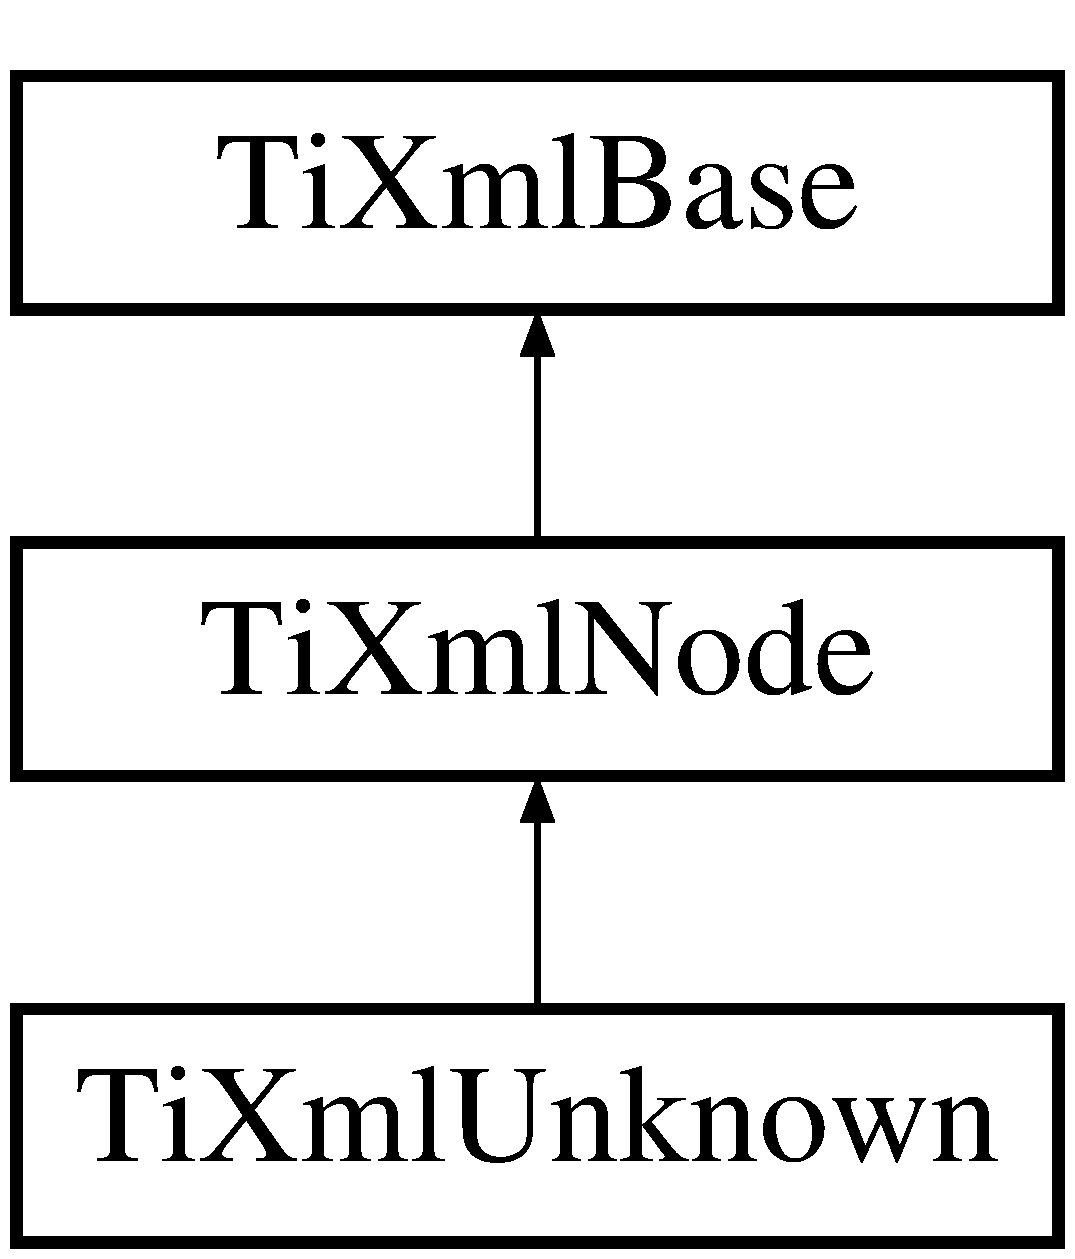
\includegraphics[height=3cm]{classTiXmlUnknown}
\end{center}
\end{figure}


\subsection{Detailed Description}
Any tag that tinyXml doesn't recognize is saved as an unknown. It is a tag of text, but should not be modified. It will be written back to the XML, unchanged, when the file is saved.

DTD tags get thrown into TiXmlUnknowns. \subsection*{Public Member Functions}
\begin{CompactItemize}
\item 
{\bf TiXmlUnknown} ()
\item 
virtual {\bf $\sim$TiXmlUnknown} ()
\item 
{\bf TiXmlUnknown} (const {\bf TiXmlUnknown} \&copy)
\item 
void {\bf operator=} (const {\bf TiXmlUnknown} \&copy)
\item 
virtual {\bf TiXmlNode} $\ast$ {\bf Clone} () const 
\begin{CompactList}\small\item\em Creates a copy of this Unknown and returns it. \item\end{CompactList}\item 
virtual void {\bf Print} (FILE $\ast$cfile, int depth) const 
\item 
virtual const char $\ast$ {\bf Parse} (const char $\ast$p, {\bf TiXmlParsingData} $\ast$data, {\bf TiXmlEncoding} encoding)
\item 
virtual const {\bf TiXmlUnknown} $\ast$ {\bf ToUnknown} () const 
\begin{CompactList}\small\item\em Cast to a more defined type. Will return null not of the requested type. \item\end{CompactList}\item 
virtual {\bf TiXmlUnknown} $\ast$ {\bf ToUnknown} ()
\begin{CompactList}\small\item\em Cast to a more defined type. Will return null not of the requested type. \item\end{CompactList}\item 
virtual bool {\bf Accept} ({\bf TiXmlVisitor} $\ast$content) const 
\end{CompactItemize}
\subsection*{Protected Member Functions}
\begin{CompactItemize}
\item 
void {\bf CopyTo} ({\bf TiXmlUnknown} $\ast$target) const 
\end{CompactItemize}


\subsection{Constructor \& Destructor Documentation}
\index{TiXmlUnknown@{TiXmlUnknown}!TiXmlUnknown@{TiXmlUnknown}}
\index{TiXmlUnknown@{TiXmlUnknown}!TiXmlUnknown@{TiXmlUnknown}}
\subsubsection{\setlength{\rightskip}{0pt plus 5cm}TiXmlUnknown::TiXmlUnknown ()\hspace{0.3cm}{\tt  [inline]}}\label{classTiXmlUnknown_945f09b3c6538099c69fc563216750c3}


\index{TiXmlUnknown@{TiXmlUnknown}!$\sim$TiXmlUnknown@{$\sim$TiXmlUnknown}}
\index{$\sim$TiXmlUnknown@{$\sim$TiXmlUnknown}!TiXmlUnknown@{TiXmlUnknown}}
\subsubsection{\setlength{\rightskip}{0pt plus 5cm}virtual TiXmlUnknown::$\sim$TiXmlUnknown ()\hspace{0.3cm}{\tt  [inline, virtual]}}\label{classTiXmlUnknown_c21966c3b551553d760b4a339c9acda0}


\index{TiXmlUnknown@{TiXmlUnknown}!TiXmlUnknown@{TiXmlUnknown}}
\index{TiXmlUnknown@{TiXmlUnknown}!TiXmlUnknown@{TiXmlUnknown}}
\subsubsection{\setlength{\rightskip}{0pt plus 5cm}TiXmlUnknown::TiXmlUnknown (const {\bf TiXmlUnknown} \& {\em copy})\hspace{0.3cm}{\tt  [inline]}}\label{classTiXmlUnknown_be798ff4feea31474850c7f0de6bdf5e}




\subsection{Member Function Documentation}
\index{TiXmlUnknown@{TiXmlUnknown}!operator=@{operator=}}
\index{operator=@{operator=}!TiXmlUnknown@{TiXmlUnknown}}
\subsubsection{\setlength{\rightskip}{0pt plus 5cm}void TiXmlUnknown::operator= (const {\bf TiXmlUnknown} \& {\em copy})\hspace{0.3cm}{\tt  [inline]}}\label{classTiXmlUnknown_5097fe228cd5ad4edcdddf02c334fd83}


\index{TiXmlUnknown@{TiXmlUnknown}!Clone@{Clone}}
\index{Clone@{Clone}!TiXmlUnknown@{TiXmlUnknown}}
\subsubsection{\setlength{\rightskip}{0pt plus 5cm}{\bf TiXmlNode} $\ast$ TiXmlUnknown::Clone () const\hspace{0.3cm}{\tt  [virtual]}}\label{classTiXmlUnknown_675c4b2684af35e4c7649b7fd5ae598d}


Creates a copy of this Unknown and returns it. 



Implements {\bf TiXmlNode} \doxyref{}{p.}{classTiXmlNode_4508cc3a2d7a98e96a54cc09c37a78a4}.\index{TiXmlUnknown@{TiXmlUnknown}!Print@{Print}}
\index{Print@{Print}!TiXmlUnknown@{TiXmlUnknown}}
\subsubsection{\setlength{\rightskip}{0pt plus 5cm}void TiXmlUnknown::Print (FILE $\ast$ {\em cfile}, int {\em depth}) const\hspace{0.3cm}{\tt  [virtual]}}\label{classTiXmlUnknown_025f19c21ef01ea9be50febb8fe0ba06}


All TinyXml classes can print themselves to a filestream or the string class (\doxyref{TiXmlString}{p.}{classTiXmlString} in non-STL mode, std::string in STL mode.) Either or both cfile and str can be null.

This is a formatted print, and will insert tabs and newlines.

(For an unformatted stream, use the $<$$<$ operator.) 

Implements {\bf TiXmlBase} \doxyref{}{p.}{classTiXmlBase_0de56b3f2ef14c65091a3b916437b512}.\index{TiXmlUnknown@{TiXmlUnknown}!Parse@{Parse}}
\index{Parse@{Parse}!TiXmlUnknown@{TiXmlUnknown}}
\subsubsection{\setlength{\rightskip}{0pt plus 5cm}const char $\ast$ TiXmlUnknown::Parse (const char $\ast$ {\em p}, {\bf TiXmlParsingData} $\ast$ {\em data}, {\bf TiXmlEncoding} {\em encoding})\hspace{0.3cm}{\tt  [virtual]}}\label{classTiXmlUnknown_a51c2694e4177b5f0b5429ee5a81b58d}




Implements {\bf TiXmlBase} \doxyref{}{p.}{classTiXmlBase_00e4edb0219d00a1379c856e5a1d2025}.\index{TiXmlUnknown@{TiXmlUnknown}!ToUnknown@{ToUnknown}}
\index{ToUnknown@{ToUnknown}!TiXmlUnknown@{TiXmlUnknown}}
\subsubsection{\setlength{\rightskip}{0pt plus 5cm}virtual const {\bf TiXmlUnknown}$\ast$ TiXmlUnknown::ToUnknown () const\hspace{0.3cm}{\tt  [inline, virtual]}}\label{classTiXmlUnknown_b0313e5fe77987d746ac1a97a254419d}


Cast to a more defined type. Will return null not of the requested type. 



Reimplemented from {\bf TiXmlNode} \doxyref{}{p.}{classTiXmlNode_fd7205cf31d7a376929f8a36930627a2}.\index{TiXmlUnknown@{TiXmlUnknown}!ToUnknown@{ToUnknown}}
\index{ToUnknown@{ToUnknown}!TiXmlUnknown@{TiXmlUnknown}}
\subsubsection{\setlength{\rightskip}{0pt plus 5cm}virtual {\bf TiXmlUnknown}$\ast$ TiXmlUnknown::ToUnknown ()\hspace{0.3cm}{\tt  [inline, virtual]}}\label{classTiXmlUnknown_67c9fd22940e8c47f706a72cdd2e332c}


Cast to a more defined type. Will return null not of the requested type. 



Reimplemented from {\bf TiXmlNode} \doxyref{}{p.}{classTiXmlNode_06de5af852668c7e4af0d09c205f0b0d}.\index{TiXmlUnknown@{TiXmlUnknown}!Accept@{Accept}}
\index{Accept@{Accept}!TiXmlUnknown@{TiXmlUnknown}}
\subsubsection{\setlength{\rightskip}{0pt plus 5cm}bool TiXmlUnknown::Accept ({\bf TiXmlVisitor} $\ast$ {\em content}) const\hspace{0.3cm}{\tt  [virtual]}}\label{classTiXmlUnknown_4e54d7482e05a837cf83c925cc683380}


Walk the XML tree visiting this node and all of its children. 

Implements {\bf TiXmlNode} \doxyref{}{p.}{classTiXmlNode_cc0f88b7462c6cb73809d410a4f5bb86}.\index{TiXmlUnknown@{TiXmlUnknown}!CopyTo@{CopyTo}}
\index{CopyTo@{CopyTo}!TiXmlUnknown@{TiXmlUnknown}}
\subsubsection{\setlength{\rightskip}{0pt plus 5cm}void TiXmlUnknown::CopyTo ({\bf TiXmlUnknown} $\ast$ {\em target}) const\hspace{0.3cm}{\tt  [protected]}}\label{classTiXmlUnknown_08ca7b225a2bcb604d3c72e199d33408}




The documentation for this class was generated from the following files:\begin{CompactItemize}
\item 
/home/msneddon/eclipse/ganymede\_\-cpp/workspace/NFsim\_\-svn/src/NFinput/TinyXML/{\bf tinyxml.h}\item 
/home/msneddon/eclipse/ganymede\_\-cpp/workspace/NFsim\_\-svn/src/NFinput/TinyXML/{\bf tinyxml.cpp}\item 
/home/msneddon/eclipse/ganymede\_\-cpp/workspace/NFsim\_\-svn/src/NFinput/TinyXML/{\bf tinyxmlparser.cpp}\end{CompactItemize}

\section{TiXmlVisitor Class Reference}
\label{classTiXmlVisitor}\index{TiXmlVisitor@{TiXmlVisitor}}
{\tt \#include $<$tinyxml.h$>$}

Inheritance diagram for TiXmlVisitor::\begin{figure}[H]
\begin{center}
\leavevmode
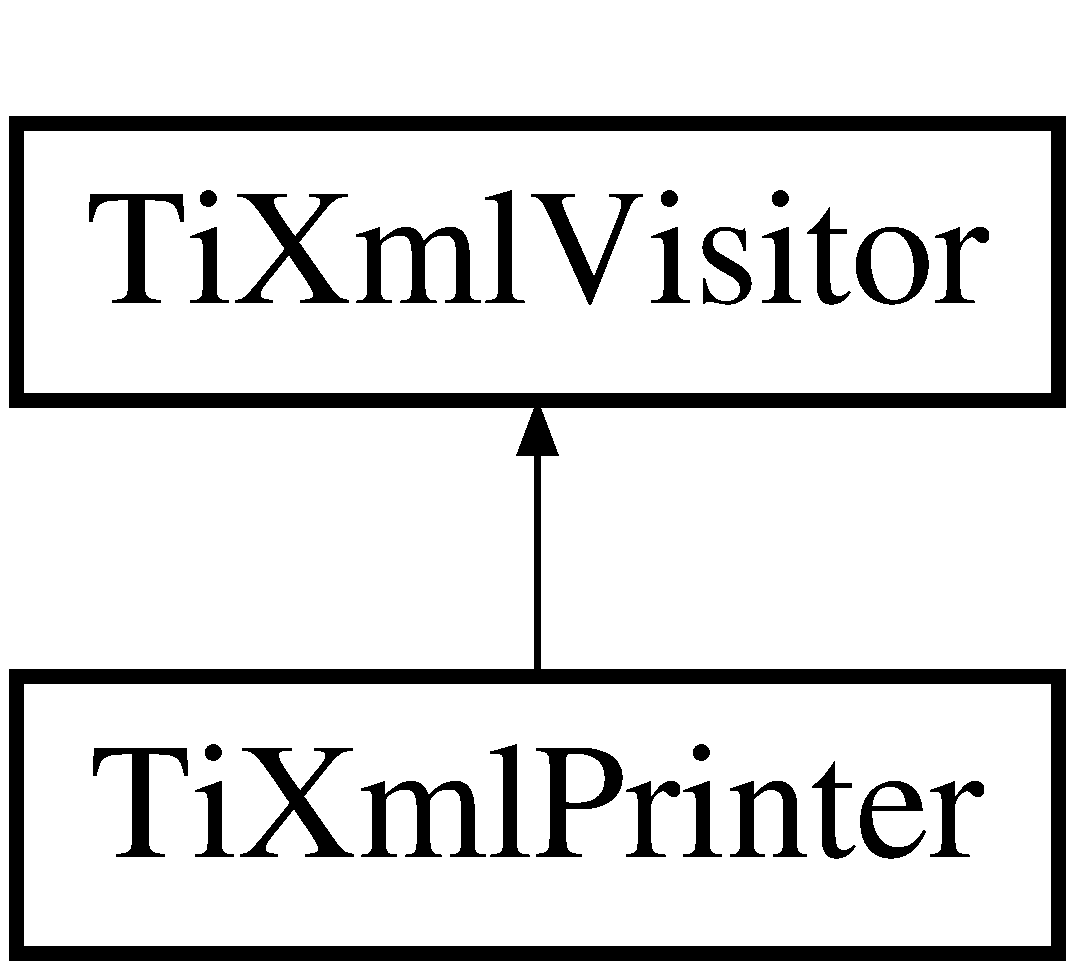
\includegraphics[height=2cm]{classTiXmlVisitor}
\end{center}
\end{figure}


\subsection{Detailed Description}
If you call the Accept() method, it requires being passed a \doxyref{TiXmlVisitor}{p.}{classTiXmlVisitor} class to handle callbacks. For nodes that contain other nodes (Document, Element) you will get called with a VisitEnter/VisitExit pair. Nodes that are always leaves are simple called with \doxyref{Visit()}{p.}{classTiXmlVisitor_fad71c71ce6473fb9b4b64cd92de4a19}.

If you return 'true' from a Visit method, recursive parsing will continue. If you return false, {\bf no children of this node or its sibilings} will be Visited.

All flavors of Visit methods have a default implementation that returns 'true' (continue visiting). You need to only override methods that are interesting to you.

Generally Accept() is called on the \doxyref{TiXmlDocument}{p.}{classTiXmlDocument}, although all nodes suppert Visiting.

You should never change the document from a callback.

\begin{Desc}
\item[See also:]\doxyref{TiXmlNode::Accept()}{p.}{classTiXmlNode_cc0f88b7462c6cb73809d410a4f5bb86} \end{Desc}
\subsection*{Public Member Functions}
\begin{CompactItemize}
\item 
virtual {\bf $\sim$TiXmlVisitor} ()
\item 
virtual bool {\bf VisitEnter} (const {\bf TiXmlDocument} \&)
\begin{CompactList}\small\item\em Visit a document. \item\end{CompactList}\item 
virtual bool {\bf VisitExit} (const {\bf TiXmlDocument} \&)
\begin{CompactList}\small\item\em Visit a document. \item\end{CompactList}\item 
virtual bool {\bf VisitEnter} (const {\bf TiXmlElement} \&, const {\bf TiXmlAttribute} $\ast$)
\begin{CompactList}\small\item\em Visit an element. \item\end{CompactList}\item 
virtual bool {\bf VisitExit} (const {\bf TiXmlElement} \&)
\begin{CompactList}\small\item\em Visit an element. \item\end{CompactList}\item 
virtual bool {\bf Visit} (const {\bf TiXmlDeclaration} \&)
\begin{CompactList}\small\item\em Visit a declaration. \item\end{CompactList}\item 
virtual bool {\bf Visit} (const {\bf TiXmlText} \&)
\begin{CompactList}\small\item\em Visit a text node. \item\end{CompactList}\item 
virtual bool {\bf Visit} (const {\bf TiXmlComment} \&)
\begin{CompactList}\small\item\em Visit a comment node. \item\end{CompactList}\item 
virtual bool {\bf Visit} (const {\bf TiXmlUnknown} \&)
\begin{CompactList}\small\item\em Visit an unknow node. \item\end{CompactList}\end{CompactItemize}


\subsection{Constructor \& Destructor Documentation}
\index{TiXmlVisitor@{TiXmlVisitor}!$\sim$TiXmlVisitor@{$\sim$TiXmlVisitor}}
\index{$\sim$TiXmlVisitor@{$\sim$TiXmlVisitor}!TiXmlVisitor@{TiXmlVisitor}}
\subsubsection{\setlength{\rightskip}{0pt plus 5cm}virtual TiXmlVisitor::$\sim$TiXmlVisitor ()\hspace{0.3cm}{\tt  [inline, virtual]}}\label{classTiXmlVisitor_276c739ec4701f27c3f86b8ead095e5a}




\subsection{Member Function Documentation}
\index{TiXmlVisitor@{TiXmlVisitor}!VisitEnter@{VisitEnter}}
\index{VisitEnter@{VisitEnter}!TiXmlVisitor@{TiXmlVisitor}}
\subsubsection{\setlength{\rightskip}{0pt plus 5cm}virtual bool TiXmlVisitor::VisitEnter (const {\bf TiXmlDocument} \&)\hspace{0.3cm}{\tt  [inline, virtual]}}\label{classTiXmlVisitor_07baecb52dd7d8716ae2a48ad0956ee0}


Visit a document. 



Reimplemented in {\bf TiXmlPrinter} \doxyref{}{p.}{classTiXmlPrinter_2ec73087db26ff4d2c4316c56f861db7}.\index{TiXmlVisitor@{TiXmlVisitor}!VisitExit@{VisitExit}}
\index{VisitExit@{VisitExit}!TiXmlVisitor@{TiXmlVisitor}}
\subsubsection{\setlength{\rightskip}{0pt plus 5cm}virtual bool TiXmlVisitor::VisitExit (const {\bf TiXmlDocument} \&)\hspace{0.3cm}{\tt  [inline, virtual]}}\label{classTiXmlVisitor_a0ade4f27087447e93974e975c3246ad}


Visit a document. 



Reimplemented in {\bf TiXmlPrinter} \doxyref{}{p.}{classTiXmlPrinter_0a636046fa589b6d7f3e5bd025b3f33e}.\index{TiXmlVisitor@{TiXmlVisitor}!VisitEnter@{VisitEnter}}
\index{VisitEnter@{VisitEnter}!TiXmlVisitor@{TiXmlVisitor}}
\subsubsection{\setlength{\rightskip}{0pt plus 5cm}virtual bool TiXmlVisitor::VisitEnter (const {\bf TiXmlElement} \&, const {\bf TiXmlAttribute} $\ast$)\hspace{0.3cm}{\tt  [inline, virtual]}}\label{classTiXmlVisitor_f6c6178ffa517bbdba95d70490875fff}


Visit an element. 



Reimplemented in {\bf TiXmlPrinter} \doxyref{}{p.}{classTiXmlPrinter_6dccaf5ee4979f13877690afe28721e8}.\index{TiXmlVisitor@{TiXmlVisitor}!VisitExit@{VisitExit}}
\index{VisitExit@{VisitExit}!TiXmlVisitor@{TiXmlVisitor}}
\subsubsection{\setlength{\rightskip}{0pt plus 5cm}virtual bool TiXmlVisitor::VisitExit (const {\bf TiXmlElement} \&)\hspace{0.3cm}{\tt  [inline, virtual]}}\label{classTiXmlVisitor_ec2b1f8116226d52f3a1b95dafd3a32c}


Visit an element. 



Reimplemented in {\bf TiXmlPrinter} \doxyref{}{p.}{classTiXmlPrinter_e6a1df8271df4bf62d7873c38e34aa69}.\index{TiXmlVisitor@{TiXmlVisitor}!Visit@{Visit}}
\index{Visit@{Visit}!TiXmlVisitor@{TiXmlVisitor}}
\subsubsection{\setlength{\rightskip}{0pt plus 5cm}virtual bool TiXmlVisitor::Visit (const {\bf TiXmlDeclaration} \&)\hspace{0.3cm}{\tt  [inline, virtual]}}\label{classTiXmlVisitor_fad71c71ce6473fb9b4b64cd92de4a19}


Visit a declaration. 



Reimplemented in {\bf TiXmlPrinter} \doxyref{}{p.}{classTiXmlPrinter_daf7eec4dc43ad071ff52b60361574f5}.\index{TiXmlVisitor@{TiXmlVisitor}!Visit@{Visit}}
\index{Visit@{Visit}!TiXmlVisitor@{TiXmlVisitor}}
\subsubsection{\setlength{\rightskip}{0pt plus 5cm}virtual bool TiXmlVisitor::Visit (const {\bf TiXmlText} \&)\hspace{0.3cm}{\tt  [inline, virtual]}}\label{classTiXmlVisitor_399b8ebca5cd14664974a32d2ce029e5}


Visit a text node. 



Reimplemented in {\bf TiXmlPrinter} \doxyref{}{p.}{classTiXmlPrinter_0857c5d32c59b9a257f9a49cb9411df5}.\index{TiXmlVisitor@{TiXmlVisitor}!Visit@{Visit}}
\index{Visit@{Visit}!TiXmlVisitor@{TiXmlVisitor}}
\subsubsection{\setlength{\rightskip}{0pt plus 5cm}virtual bool TiXmlVisitor::Visit (const {\bf TiXmlComment} \&)\hspace{0.3cm}{\tt  [inline, virtual]}}\label{classTiXmlVisitor_53a60e7a528627b31af3161972cc7fa2}


Visit a comment node. 



Reimplemented in {\bf TiXmlPrinter} \doxyref{}{p.}{classTiXmlPrinter_9870423f5603630e6142f6bdb66dfb57}.\index{TiXmlVisitor@{TiXmlVisitor}!Visit@{Visit}}
\index{Visit@{Visit}!TiXmlVisitor@{TiXmlVisitor}}
\subsubsection{\setlength{\rightskip}{0pt plus 5cm}virtual bool TiXmlVisitor::Visit (const {\bf TiXmlUnknown} \&)\hspace{0.3cm}{\tt  [inline, virtual]}}\label{classTiXmlVisitor_7e284d607d275c51dac1adb58159ce28}


Visit an unknow node. 



Reimplemented in {\bf TiXmlPrinter} \doxyref{}{p.}{classTiXmlPrinter_08591a15c9a07afa83c24e08b03d6358}.

The documentation for this class was generated from the following file:\begin{CompactItemize}
\item 
/home/msneddon/eclipse/galileoSR1\_\-cpp/workspace/NFsim/src/NFinput/TinyXML/{\bf tinyxml.h}\end{CompactItemize}

\section{NFcore::Transformation Class Reference}
\label{classNFcore_1_1Transformation}\index{NFcore::Transformation@{NFcore::Transformation}}
{\tt \#include $<$transformation.hh$>$}

Inheritance diagram for NFcore::Transformation::\begin{figure}[H]
\begin{center}
\leavevmode
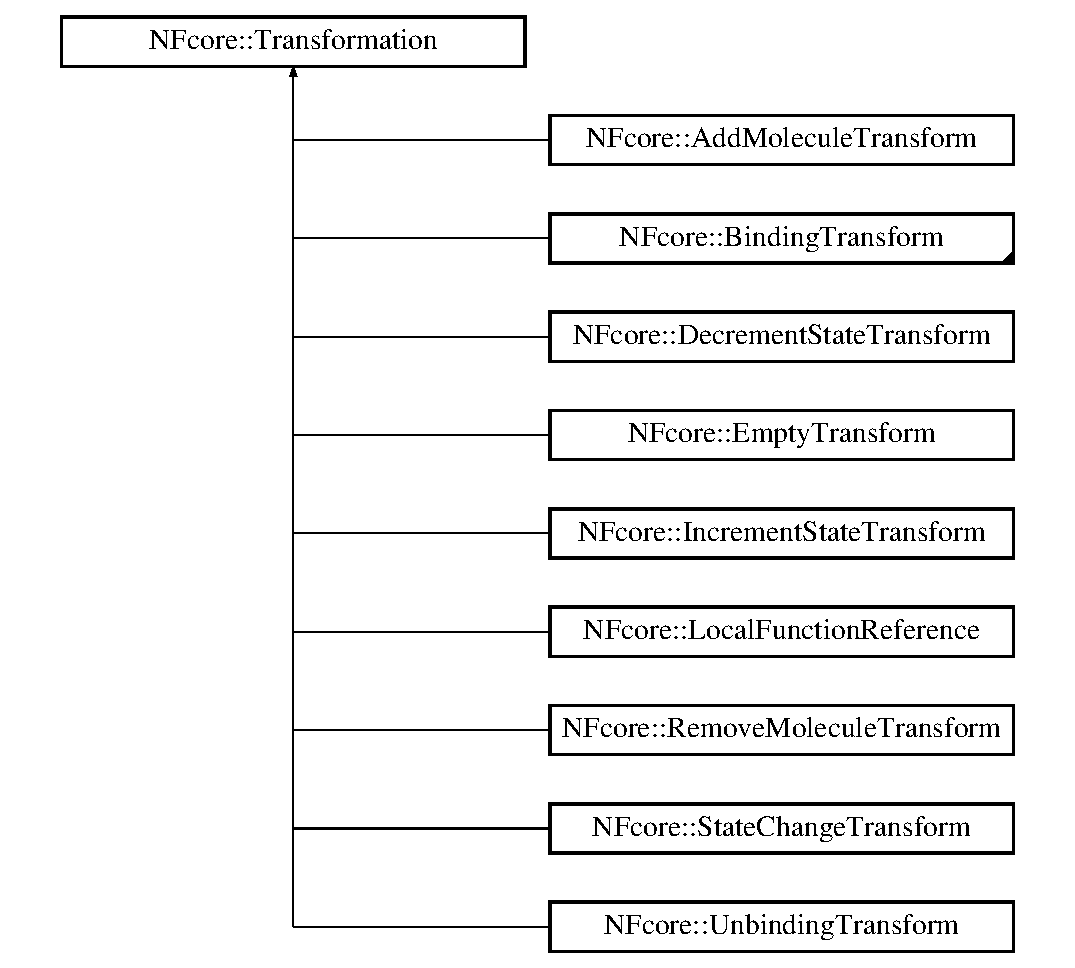
\includegraphics[height=10cm]{classNFcore_1_1Transformation}
\end{center}
\end{figure}


\subsection{Detailed Description}
Abstract transformation object that other types of transformations inherit from. \begin{Desc}
\item[Author:]Michael Sneddon \end{Desc}
\subsection*{Public Member Functions}
\begin{CompactItemize}
\item 
{\bf Transformation} (int {\bf type})
\item 
virtual {\bf $\sim$Transformation} ()
\item 
int {\bf getType} () const 
\item 
virtual void {\bf apply} ({\bf Mapping} $\ast$m, {\bf MappingSet} $\ast$$\ast$ms)=0
\item 
virtual int {\bf getComponentIndex} () const =0
\item 
virtual int {\bf getRemovalType} ()
\end{CompactItemize}
\subsection*{Protected Attributes}
\begin{CompactItemize}
\item 
int {\bf type}
\end{CompactItemize}


\subsection{Constructor \& Destructor Documentation}
\index{NFcore::Transformation@{NFcore::Transformation}!Transformation@{Transformation}}
\index{Transformation@{Transformation}!NFcore::Transformation@{NFcore::Transformation}}
\subsubsection{\setlength{\rightskip}{0pt plus 5cm}NFcore::Transformation::Transformation (int {\em type})\hspace{0.3cm}{\tt  [inline]}}\label{classNFcore_1_1Transformation_4e8e9f52348d9116d44a290a64117280}


\index{NFcore::Transformation@{NFcore::Transformation}!$\sim$Transformation@{$\sim$Transformation}}
\index{$\sim$Transformation@{$\sim$Transformation}!NFcore::Transformation@{NFcore::Transformation}}
\subsubsection{\setlength{\rightskip}{0pt plus 5cm}virtual NFcore::Transformation::$\sim$Transformation ()\hspace{0.3cm}{\tt  [inline, virtual]}}\label{classNFcore_1_1Transformation_12c1222abdec2d650a1f0c05378afd47}




\subsection{Member Function Documentation}
\index{NFcore::Transformation@{NFcore::Transformation}!getType@{getType}}
\index{getType@{getType}!NFcore::Transformation@{NFcore::Transformation}}
\subsubsection{\setlength{\rightskip}{0pt plus 5cm}int NFcore::Transformation::getType () const\hspace{0.3cm}{\tt  [inline]}}\label{classNFcore_1_1Transformation_ad557022a9df81b8009ee0230cbd901e}


\index{NFcore::Transformation@{NFcore::Transformation}!apply@{apply}}
\index{apply@{apply}!NFcore::Transformation@{NFcore::Transformation}}
\subsubsection{\setlength{\rightskip}{0pt plus 5cm}virtual void NFcore::Transformation::apply ({\bf Mapping} $\ast$ {\em m}, {\bf MappingSet} $\ast$$\ast$ {\em ms})\hspace{0.3cm}{\tt  [pure virtual]}}\label{classNFcore_1_1Transformation_6a57f607676c92b2465427e57bc7fae5}




Implemented in {\bf NFcore::LocalFunctionReference} \doxyref{}{p.}{classNFcore_1_1LocalFunctionReference_62280a5922e15fcda20b801ca2662ba8}, {\bf NFcore::EmptyTransform} \doxyref{}{p.}{classNFcore_1_1EmptyTransform_fd2dd5c89bfd563a2343a9a40a3a21b1}, {\bf NFcore::StateChangeTransform} \doxyref{}{p.}{classNFcore_1_1StateChangeTransform_a74df84e5d6eac3709ea4636a674edee}, {\bf NFcore::BindingTransform} \doxyref{}{p.}{classNFcore_1_1BindingTransform_45f7022ec7b76e0ba90021de650026e9}, {\bf NFcore::BindingSeparateComplexTransform} \doxyref{}{p.}{classNFcore_1_1BindingSeparateComplexTransform_af8be6214ca8a9a4041754bb3189ca09}, {\bf NFcore::UnbindingTransform} \doxyref{}{p.}{classNFcore_1_1UnbindingTransform_bc0ad11a6deed270f892cc2c072f016d}, {\bf NFcore::AddMoleculeTransform} \doxyref{}{p.}{classNFcore_1_1AddMoleculeTransform_18b5845ce1e6d9c249acc40ff7b49dfd}, {\bf NFcore::RemoveMoleculeTransform} \doxyref{}{p.}{classNFcore_1_1RemoveMoleculeTransform_c277e491df71ad554a93e93ad1e02a7a}, {\bf NFcore::IncrementStateTransform} \doxyref{}{p.}{classNFcore_1_1IncrementStateTransform_47ec72e990cfad2110e251b2749e6a34}, and {\bf NFcore::DecrementStateTransform} \doxyref{}{p.}{classNFcore_1_1DecrementStateTransform_2094268f2958cc380cc9ec1c8a8332da}.\index{NFcore::Transformation@{NFcore::Transformation}!getComponentIndex@{getComponentIndex}}
\index{getComponentIndex@{getComponentIndex}!NFcore::Transformation@{NFcore::Transformation}}
\subsubsection{\setlength{\rightskip}{0pt plus 5cm}virtual int NFcore::Transformation::getComponentIndex () const\hspace{0.3cm}{\tt  [pure virtual]}}\label{classNFcore_1_1Transformation_2ba394b20768b21ba328431103474607}




Implemented in {\bf NFcore::LocalFunctionReference} \doxyref{}{p.}{classNFcore_1_1LocalFunctionReference_fad70297f131516af5b68ef5f508dfc9}, {\bf NFcore::EmptyTransform} \doxyref{}{p.}{classNFcore_1_1EmptyTransform_7263f704ef8b0fe2388da3379880df4d}, {\bf NFcore::StateChangeTransform} \doxyref{}{p.}{classNFcore_1_1StateChangeTransform_5ae788f00d608b4d4417408d2559a0fb}, {\bf NFcore::BindingTransform} \doxyref{}{p.}{classNFcore_1_1BindingTransform_9dad3bcc59c0c0dfd316fc494b7689be}, {\bf NFcore::BindingSeparateComplexTransform} \doxyref{}{p.}{classNFcore_1_1BindingSeparateComplexTransform_5ea6920bf3d0a5fb624cff52cf0c97ce}, {\bf NFcore::UnbindingTransform} \doxyref{}{p.}{classNFcore_1_1UnbindingTransform_d0f5ce90812bad1d25a8b3de001f04d7}, {\bf NFcore::AddMoleculeTransform} \doxyref{}{p.}{classNFcore_1_1AddMoleculeTransform_8a352eb7aa54568e417701461d507b9e}, {\bf NFcore::RemoveMoleculeTransform} \doxyref{}{p.}{classNFcore_1_1RemoveMoleculeTransform_02344a04ae5aa77f01786cb88cbe1185}, {\bf NFcore::IncrementStateTransform} \doxyref{}{p.}{classNFcore_1_1IncrementStateTransform_c43495e0e7ad7ef79ad7bd8dfb940825}, and {\bf NFcore::DecrementStateTransform} \doxyref{}{p.}{classNFcore_1_1DecrementStateTransform_8609049e75d2a31fb64c32f1608565bf}.\index{NFcore::Transformation@{NFcore::Transformation}!getRemovalType@{getRemovalType}}
\index{getRemovalType@{getRemovalType}!NFcore::Transformation@{NFcore::Transformation}}
\subsubsection{\setlength{\rightskip}{0pt plus 5cm}virtual int NFcore::Transformation::getRemovalType ()\hspace{0.3cm}{\tt  [inline, virtual]}}\label{classNFcore_1_1Transformation_d664f83913869feb14f2bd80b6851311}




Reimplemented in {\bf NFcore::RemoveMoleculeTransform} \doxyref{}{p.}{classNFcore_1_1RemoveMoleculeTransform_5dccf8d515fd99ab849dd13e7c4ccef1}.

\subsection{Member Data Documentation}
\index{NFcore::Transformation@{NFcore::Transformation}!type@{type}}
\index{type@{type}!NFcore::Transformation@{NFcore::Transformation}}
\subsubsection{\setlength{\rightskip}{0pt plus 5cm}int {\bf NFcore::Transformation::type}\hspace{0.3cm}{\tt  [protected]}}\label{classNFcore_1_1Transformation_4ce8adc1b4dde8c4dcfd4c3b4ce1b64a}




The documentation for this class was generated from the following file:\begin{CompactItemize}
\item 
/home/msneddon/eclipse/galileoSR1\_\-cpp/workspace/NFsim/src/NFreactions/transformations/{\bf transformation.hh}\end{CompactItemize}

\section{NFcore::TransformationFactory Class Reference}
\label{classNFcore_1_1TransformationFactory}\index{NFcore::TransformationFactory@{NFcore::TransformationFactory}}
{\tt \#include $<$transformation.hh$>$}

\subsection*{Static Public Member Functions}
\begin{CompactItemize}
\item 
static {\bf Transformation} $\ast$ {\bf genStateChangeTransform} (unsigned int cIndex, int newValue)
\item 
static {\bf Transformation} $\ast$ {\bf genBindingTransform1} (unsigned int bSiteIndex, unsigned int otherReactantIndex, unsigned int otherMappingIndex)
\item 
static {\bf Transformation} $\ast$ {\bf genBindingSeparateComplexTransform1} (unsigned int bSiteIndex, unsigned int otherReactantIndex, unsigned int otherMappingIndex)
\item 
static {\bf Transformation} $\ast$ {\bf genBindingTransform2} (unsigned int bSiteIndex)
\item 
static {\bf Transformation} $\ast$ {\bf genUnbindingTransform} (unsigned int bSiteIndex)
\item 
static {\bf Transformation} $\ast$ {\bf genAddMoleculeTransform} ({\bf SpeciesCreator} $\ast$sc)
\item 
static {\bf Transformation} $\ast$ {\bf genRemoveMoleculeTransform} ()
\item 
static {\bf Transformation} $\ast$ {\bf genEmptyTransform} ()
\item 
static {\bf Transformation} $\ast$ {\bf genIncrementStateTransform} (unsigned int cIndex)
\item 
static {\bf Transformation} $\ast$ {\bf genDecrementStateTransform} (unsigned int cIndex)
\item 
static {\bf Transformation} $\ast$ {\bf genLocalFunctionReference} (string PointerName, int type, {\bf TemplateMolecule} $\ast$tm)
\end{CompactItemize}
\subsection*{Static Public Attributes}
\begin{CompactItemize}
\item 
static const unsigned int {\bf STATE\_\-CHANGE} = 0
\item 
static const unsigned int {\bf BINDING} = 1
\item 
static const unsigned int {\bf UNBINDING} = 2
\item 
static const unsigned int {\bf REMOVE} = 3
\item 
static const unsigned int {\bf ADD} = 4
\item 
static const unsigned int {\bf EMPTY} = 5
\item 
static const unsigned int {\bf INCREMENT\_\-STATE} = 6
\item 
static const unsigned int {\bf DECREMENT\_\-STATE} = 7
\item 
static const unsigned int {\bf LOCAL\_\-FUNCTION\_\-REFERENCE} = 8
\end{CompactItemize}


\subsection{Member Function Documentation}
\index{NFcore::TransformationFactory@{NFcore::TransformationFactory}!genStateChangeTransform@{genStateChangeTransform}}
\index{genStateChangeTransform@{genStateChangeTransform}!NFcore::TransformationFactory@{NFcore::TransformationFactory}}
\subsubsection{\setlength{\rightskip}{0pt plus 5cm}{\bf NFcore::Transformation} $\ast$ TransformationFactory::genStateChangeTransform (unsigned int {\em cIndex}, int {\em newValue})\hspace{0.3cm}{\tt  [static]}}\label{classNFcore_1_1TransformationFactory_c8a9523b24c856ab84f106a8740d2baf}


Generates a state change \doxyref{Transformation}{p.}{classNFcore_1_1Transformation} for transforming the given state at the given index into the new state value. \begin{Desc}
\item[Author:]Michael Sneddon \end{Desc}
\index{NFcore::TransformationFactory@{NFcore::TransformationFactory}!genBindingTransform1@{genBindingTransform1}}
\index{genBindingTransform1@{genBindingTransform1}!NFcore::TransformationFactory@{NFcore::TransformationFactory}}
\subsubsection{\setlength{\rightskip}{0pt plus 5cm}{\bf NFcore::Transformation} $\ast$ TransformationFactory::genBindingTransform1 (unsigned int {\em bSiteIndex}, unsigned int {\em otherReactantIndex}, unsigned int {\em otherMappingIndex})\hspace{0.3cm}{\tt  [static]}}\label{classNFcore_1_1TransformationFactory_b43cb8fbbaa03e4edd9366bc922f9c2c}


Generates a binding transformation for one of the two binding sites in the binding Transform. You will have to tell it where the other \doxyref{Transformation}{p.}{classNFcore_1_1Transformation} object lives (\doxyref{TransformationSet}{p.}{classNFcore_1_1TransformationSet} has this information). \begin{Desc}
\item[Author:]Michael Sneddon \end{Desc}
\index{NFcore::TransformationFactory@{NFcore::TransformationFactory}!genBindingSeparateComplexTransform1@{genBindingSeparateComplexTransform1}}
\index{genBindingSeparateComplexTransform1@{genBindingSeparateComplexTransform1}!NFcore::TransformationFactory@{NFcore::TransformationFactory}}
\subsubsection{\setlength{\rightskip}{0pt plus 5cm}{\bf NFcore::Transformation} $\ast$ TransformationFactory::genBindingSeparateComplexTransform1 (unsigned int {\em bSiteIndex}, unsigned int {\em otherReactantIndex}, unsigned int {\em otherMappingIndex})\hspace{0.3cm}{\tt  [static]}}\label{classNFcore_1_1TransformationFactory_275722d56c36dfe9be8e8cca8fcc4fab}


\index{NFcore::TransformationFactory@{NFcore::TransformationFactory}!genBindingTransform2@{genBindingTransform2}}
\index{genBindingTransform2@{genBindingTransform2}!NFcore::TransformationFactory@{NFcore::TransformationFactory}}
\subsubsection{\setlength{\rightskip}{0pt plus 5cm}{\bf NFcore::Transformation} $\ast$ TransformationFactory::genBindingTransform2 (unsigned int {\em bSiteIndex})\hspace{0.3cm}{\tt  [static]}}\label{classNFcore_1_1TransformationFactory_60536e9fb733aa835613410f1cf3ec25}


Generates the second half of a binding transform. The other site already knows about this site, so all you need here is the index of the binding site that must be bonded. \begin{Desc}
\item[Author:]Michael Sneddon \end{Desc}
\index{NFcore::TransformationFactory@{NFcore::TransformationFactory}!genUnbindingTransform@{genUnbindingTransform}}
\index{genUnbindingTransform@{genUnbindingTransform}!NFcore::TransformationFactory@{NFcore::TransformationFactory}}
\subsubsection{\setlength{\rightskip}{0pt plus 5cm}{\bf NFcore::Transformation} $\ast$ TransformationFactory::genUnbindingTransform (unsigned int {\em bSiteIndex})\hspace{0.3cm}{\tt  [static]}}\label{classNFcore_1_1TransformationFactory_6d0b9445e9c48c59f807c727445054ab}


Generates an unbinding transformation for a particular binding site. Only one of the binding sites must be specified as a \doxyref{Transformation}{p.}{classNFcore_1_1Transformation} - the other is automatically taken care of. \begin{Desc}
\item[Author:]Michael Sneddon \end{Desc}
\index{NFcore::TransformationFactory@{NFcore::TransformationFactory}!genAddMoleculeTransform@{genAddMoleculeTransform}}
\index{genAddMoleculeTransform@{genAddMoleculeTransform}!NFcore::TransformationFactory@{NFcore::TransformationFactory}}
\subsubsection{\setlength{\rightskip}{0pt plus 5cm}{\bf NFcore::Transformation} $\ast$ TransformationFactory::genAddMoleculeTransform ({\bf SpeciesCreator} $\ast$ {\em sc})\hspace{0.3cm}{\tt  [static]}}\label{classNFcore_1_1TransformationFactory_f11322a3ba45cabe38b2eadf032a1ff6}


Generates an Add \doxyref{Molecule}{p.}{classNFcore_1_1Molecule} transformation. Currently, this is not yet implemented. \begin{Desc}
\item[Author:]Michael Sneddon \end{Desc}
\index{NFcore::TransformationFactory@{NFcore::TransformationFactory}!genRemoveMoleculeTransform@{genRemoveMoleculeTransform}}
\index{genRemoveMoleculeTransform@{genRemoveMoleculeTransform}!NFcore::TransformationFactory@{NFcore::TransformationFactory}}
\subsubsection{\setlength{\rightskip}{0pt plus 5cm}{\bf NFcore::Transformation} $\ast$ TransformationFactory::genRemoveMoleculeTransform ()\hspace{0.3cm}{\tt  [static]}}\label{classNFcore_1_1TransformationFactory_5d848169fa346fc9642cc34ecf706ea3}


Generates a removal of a molecule from the system. Currently this is not yet implemented. \begin{Desc}
\item[Author:]Michael Sneddon \end{Desc}
\index{NFcore::TransformationFactory@{NFcore::TransformationFactory}!genEmptyTransform@{genEmptyTransform}}
\index{genEmptyTransform@{genEmptyTransform}!NFcore::TransformationFactory@{NFcore::TransformationFactory}}
\subsubsection{\setlength{\rightskip}{0pt plus 5cm}{\bf NFcore::Transformation} $\ast$ TransformationFactory::genEmptyTransform ()\hspace{0.3cm}{\tt  [static]}}\label{classNFcore_1_1TransformationFactory_4bcd9f929fb6c17f6935dea191e9e9aa}


Generates an empty transformation. This is used in cases where there is a reactant that is not transformed in a reaction, but that still needs to be counted and marked so that the rate of the reaction is correct. \begin{Desc}
\item[Author:]Michael Sneddon \end{Desc}
\index{NFcore::TransformationFactory@{NFcore::TransformationFactory}!genIncrementStateTransform@{genIncrementStateTransform}}
\index{genIncrementStateTransform@{genIncrementStateTransform}!NFcore::TransformationFactory@{NFcore::TransformationFactory}}
\subsubsection{\setlength{\rightskip}{0pt plus 5cm}{\bf NFcore::Transformation} $\ast$ TransformationFactory::genIncrementStateTransform (unsigned int {\em cIndex})\hspace{0.3cm}{\tt  [static]}}\label{classNFcore_1_1TransformationFactory_250f200fbcc8e794b8b99cc45302ab3b}


Generates an IncrementState transformation. \begin{Desc}
\item[Author:]Michael Sneddon \end{Desc}
\index{NFcore::TransformationFactory@{NFcore::TransformationFactory}!genDecrementStateTransform@{genDecrementStateTransform}}
\index{genDecrementStateTransform@{genDecrementStateTransform}!NFcore::TransformationFactory@{NFcore::TransformationFactory}}
\subsubsection{\setlength{\rightskip}{0pt plus 5cm}{\bf NFcore::Transformation} $\ast$ TransformationFactory::genDecrementStateTransform (unsigned int {\em cIndex})\hspace{0.3cm}{\tt  [static]}}\label{classNFcore_1_1TransformationFactory_eece84f71547208fa9e27ecda1032489}


Generates an DecrementState transformation. \begin{Desc}
\item[Author:]Michael Sneddon \end{Desc}
\index{NFcore::TransformationFactory@{NFcore::TransformationFactory}!genLocalFunctionReference@{genLocalFunctionReference}}
\index{genLocalFunctionReference@{genLocalFunctionReference}!NFcore::TransformationFactory@{NFcore::TransformationFactory}}
\subsubsection{\setlength{\rightskip}{0pt plus 5cm}{\bf Transformation} $\ast$ TransformationFactory::genLocalFunctionReference (string {\em PointerName}, int {\em type}, {\bf TemplateMolecule} $\ast$ {\em tm})\hspace{0.3cm}{\tt  [static]}}\label{classNFcore_1_1TransformationFactory_206a59330bba84e1b0131b8b0ba919f4}




\subsection{Member Data Documentation}
\index{NFcore::TransformationFactory@{NFcore::TransformationFactory}!STATE\_\-CHANGE@{STATE\_\-CHANGE}}
\index{STATE\_\-CHANGE@{STATE\_\-CHANGE}!NFcore::TransformationFactory@{NFcore::TransformationFactory}}
\subsubsection{\setlength{\rightskip}{0pt plus 5cm}const unsigned int {\bf NFcore::TransformationFactory::STATE\_\-CHANGE} = 0\hspace{0.3cm}{\tt  [static]}}\label{classNFcore_1_1TransformationFactory_5b83f8ccba33c9c11d57ccb01eb65b8b}


Indicates a state change transformation or mapping onto a state \index{NFcore::TransformationFactory@{NFcore::TransformationFactory}!BINDING@{BINDING}}
\index{BINDING@{BINDING}!NFcore::TransformationFactory@{NFcore::TransformationFactory}}
\subsubsection{\setlength{\rightskip}{0pt plus 5cm}const unsigned int {\bf NFcore::TransformationFactory::BINDING} = 1\hspace{0.3cm}{\tt  [static]}}\label{classNFcore_1_1TransformationFactory_9d39c00ef66f1a76c2d0d466753382e6}


Indicates a binding transformation or mapping onto a binding site \index{NFcore::TransformationFactory@{NFcore::TransformationFactory}!UNBINDING@{UNBINDING}}
\index{UNBINDING@{UNBINDING}!NFcore::TransformationFactory@{NFcore::TransformationFactory}}
\subsubsection{\setlength{\rightskip}{0pt plus 5cm}const unsigned int {\bf NFcore::TransformationFactory::UNBINDING} = 2\hspace{0.3cm}{\tt  [static]}}\label{classNFcore_1_1TransformationFactory_b7940a37633cc5c84bb5d8e7181cda04}


Indicates an unbinding transformation or mapping onto a binding site \index{NFcore::TransformationFactory@{NFcore::TransformationFactory}!REMOVE@{REMOVE}}
\index{REMOVE@{REMOVE}!NFcore::TransformationFactory@{NFcore::TransformationFactory}}
\subsubsection{\setlength{\rightskip}{0pt plus 5cm}const unsigned int {\bf NFcore::TransformationFactory::REMOVE} = 3\hspace{0.3cm}{\tt  [static]}}\label{classNFcore_1_1TransformationFactory_5a5169186f10927cf62a9a542d1b1b95}


Indicates a removal transform or mapping onto an entire \doxyref{Molecule}{p.}{classNFcore_1_1Molecule} \index{NFcore::TransformationFactory@{NFcore::TransformationFactory}!ADD@{ADD}}
\index{ADD@{ADD}!NFcore::TransformationFactory@{NFcore::TransformationFactory}}
\subsubsection{\setlength{\rightskip}{0pt plus 5cm}const unsigned int {\bf NFcore::TransformationFactory::ADD} = 4\hspace{0.3cm}{\tt  [static]}}\label{classNFcore_1_1TransformationFactory_492322bf2daa6a96dca1bb1b13d7a1d5}


Indicates an addition transform \index{NFcore::TransformationFactory@{NFcore::TransformationFactory}!EMPTY@{EMPTY}}
\index{EMPTY@{EMPTY}!NFcore::TransformationFactory@{NFcore::TransformationFactory}}
\subsubsection{\setlength{\rightskip}{0pt plus 5cm}const unsigned int {\bf NFcore::TransformationFactory::EMPTY} = 5\hspace{0.3cm}{\tt  [static]}}\label{classNFcore_1_1TransformationFactory_6248b102fcc6990bfbca65d3dfa4764e}


Indicates no transformation is needed (or is the second partner in a binding transform and so should be skipped when applying transforms \index{NFcore::TransformationFactory@{NFcore::TransformationFactory}!INCREMENT\_\-STATE@{INCREMENT\_\-STATE}}
\index{INCREMENT\_\-STATE@{INCREMENT\_\-STATE}!NFcore::TransformationFactory@{NFcore::TransformationFactory}}
\subsubsection{\setlength{\rightskip}{0pt plus 5cm}const unsigned int {\bf NFcore::TransformationFactory::INCREMENT\_\-STATE} = 6\hspace{0.3cm}{\tt  [static]}}\label{classNFcore_1_1TransformationFactory_bb9132a59d041a40b6503fffc37e51c5}


\index{NFcore::TransformationFactory@{NFcore::TransformationFactory}!DECREMENT\_\-STATE@{DECREMENT\_\-STATE}}
\index{DECREMENT\_\-STATE@{DECREMENT\_\-STATE}!NFcore::TransformationFactory@{NFcore::TransformationFactory}}
\subsubsection{\setlength{\rightskip}{0pt plus 5cm}const unsigned int {\bf NFcore::TransformationFactory::DECREMENT\_\-STATE} = 7\hspace{0.3cm}{\tt  [static]}}\label{classNFcore_1_1TransformationFactory_ef1bf254664f1baaa23127355a427fde}


\index{NFcore::TransformationFactory@{NFcore::TransformationFactory}!LOCAL\_\-FUNCTION\_\-REFERENCE@{LOCAL\_\-FUNCTION\_\-REFERENCE}}
\index{LOCAL\_\-FUNCTION\_\-REFERENCE@{LOCAL\_\-FUNCTION\_\-REFERENCE}!NFcore::TransformationFactory@{NFcore::TransformationFactory}}
\subsubsection{\setlength{\rightskip}{0pt plus 5cm}const unsigned int {\bf NFcore::TransformationFactory::LOCAL\_\-FUNCTION\_\-REFERENCE} = 8\hspace{0.3cm}{\tt  [static]}}\label{classNFcore_1_1TransformationFactory_2082f8fc11ff7315d0454c2bf61bf0e4}




The documentation for this class was generated from the following files:\begin{CompactItemize}
\item 
/home/msneddon/eclipse/ganymede\_\-cpp/workspace/NFsim\_\-svn/src/NFreactions/transformations/{\bf transformation.hh}\item 
/home/msneddon/eclipse/ganymede\_\-cpp/workspace/NFsim\_\-svn/src/NFreactions/transformations/{\bf transformation.cpp}\end{CompactItemize}

\section{NFcore::TransformationSet Class Reference}
\label{classNFcore_1_1TransformationSet}\index{NFcore::TransformationSet@{NFcore::TransformationSet}}
{\tt \#include $<$transformationSet.hh$>$}



\subsection{Detailed Description}
Maintains a set of \doxyref{Transformation}{p.}{classNFcore_1_1Transformation} objects for a \doxyref{ReactionClass}{p.}{classNFcore_1_1ReactionClass}. 

This class is one of the core pieces of a \doxyref{ReactionClass}{p.}{classNFcore_1_1ReactionClass}. It maintains the set of \doxyref{Transformation}{p.}{classNFcore_1_1Transformation} objects for each of the reactants in the \doxyref{ReactionClass}{p.}{classNFcore_1_1ReactionClass}. Therefore, it knows about the TemplateMolecules of the \doxyref{ReactionClass}{p.}{classNFcore_1_1ReactionClass}; it knows how to generate \doxyref{MappingSet}{p.}{classNFcore_1_1MappingSet} objects for the ReactantLists; it knows how to create MappingGenerator objects for TemplateMolecules; it knows how to execute the set of Transformations; and finally, it knows how to generate the list of product molecules that are generated from firing a reaction rule. To use this class, first create your \doxyref{TemplateMolecule}{p.}{classNFcore_1_1TemplateMolecule} objects for your \doxyref{ReactionClass}{p.}{classNFcore_1_1ReactionClass}. Create a \doxyref{TransformationSet}{p.}{classNFcore_1_1TransformationSet} from the \doxyref{TemplateMolecule}{p.}{classNFcore_1_1TemplateMolecule} vector (the vector should be created such that each element of the vector is a reactant in the \doxyref{ReactionClass}{p.}{classNFcore_1_1ReactionClass}). Add as many Transformations to the set as you like using the \doxyref{TransformationSet}{p.}{classNFcore_1_1TransformationSet} static functions. Finally, call the \doxyref{finalize()}{p.}{classNFcore_1_1TransformationSet_ff4b1c7450529960cd211ef1949a479f} function to finish setting upt the \doxyref{TransformationSet}{p.}{classNFcore_1_1TransformationSet}. Then you can use this \doxyref{TransformationSet}{p.}{classNFcore_1_1TransformationSet} to create a \doxyref{ReactionClass}{p.}{classNFcore_1_1ReactionClass} with ease. Really, this is all easier than it sounds! (see \doxyref{simple\_\-system.hh}{p.}{simple__system_8hh} and \doxyref{simple\_\-system.cpp}{p.}{simple__system_8cpp} ) \begin{Desc}
\item[Author:]Michael Sneddon \end{Desc}
\subsection*{Public Member Functions}
\begin{CompactItemize}
\item 
{\bf TransformationSet} (vector$<$ {\bf TemplateMolecule} $\ast$ $>$ reactantTemplates)
\item 
{\bf TransformationSet} (vector$<$ {\bf TemplateMolecule} $\ast$ $>$ reactantTemplates, vector$<$ {\bf TemplateMolecule} $\ast$ $>$ addMoleculeTemplates)
\item 
{\bf $\sim$TransformationSet} ()
\item 
int {\bf getNumOfReactants} () const 
\item 
bool {\bf addStateChangeTransform} ({\bf TemplateMolecule} $\ast$t, string cName, int finalStateValue)
\item 
bool {\bf addStateChangeTransform} ({\bf TemplateMolecule} $\ast$t, string cName, string finalStateValue)
\item 
bool {\bf addIncrementStateTransform} ({\bf TemplateMolecule} $\ast$t, string cName)
\item 
bool {\bf addDecrementStateTransform} ({\bf TemplateMolecule} $\ast$t, string cName)
\item 
bool {\bf addBindingTransform} ({\bf TemplateMolecule} $\ast$t1, string bSiteName1, {\bf TemplateMolecule} $\ast$t2, string bSiteName2)
\item 
bool {\bf addNewMoleculeBindingTransform} ({\bf TemplateMolecule} $\ast$t1, string bSiteName1, {\bf TemplateMolecule} $\ast$t2, string bSiteName2)
\item 
bool {\bf addBindingSeparateComplexTransform} ({\bf TemplateMolecule} $\ast$t1, string bSiteName1, {\bf TemplateMolecule} $\ast$t2, string bSiteName2)
\item 
bool {\bf addUnbindingTransform} ({\bf TemplateMolecule} $\ast$t, string bSiteName, {\bf TemplateMolecule} $\ast$t2, string bSiteName2)
\item 
bool {\bf addDeleteMolecule} ({\bf TemplateMolecule} $\ast$t, int deletionType)
\item 
bool {\bf addDecrementPopulation} ({\bf TemplateMolecule} $\ast$t)
\item 
bool {\bf addAddSpecies} ({\bf SpeciesCreator} $\ast$sc)
\item 
bool {\bf addAddMolecule} ({\bf MoleculeCreator} $\ast$mc)
\item 
bool {\bf addLocalFunctionReference} ({\bf TemplateMolecule} $\ast$t, string PointerName, int scope)
\item 
bool {\bf transform} ({\bf MappingSet} $\ast$$\ast$mappingSets)
\item 
{\bf MappingSet} $\ast$ {\bf generateBlankMappingSet} (unsigned int reactantIndex, unsigned int mappingSetId)
\item 
{\bf TemplateMolecule} $\ast$ {\bf getTemplateMolecule} (unsigned int reactantIndex) const 
\item 
unsigned int {\bf getNreactants} () const 
\item 
unsigned int {\bf getNmappingSets} () const 
\item 
bool {\bf getComplexBookkeeping} () const 
\item 
void {\bf setComplexBookkeeping} (bool val)
\item 
void {\bf finalize} ()
\item 
bool {\bf isFinalized} () const 
\item 
bool {\bf checkMolecularity} ({\bf MappingSet} $\ast$$\ast$mappingSets)
\item 
bool {\bf getListOfProducts} ({\bf MappingSet} $\ast$$\ast$mappingSets, list$<$ {\bf Molecule} $\ast$ $>$ \&products, int traversalLimit)
\item 
bool {\bf getListOfAddedMolecules} ({\bf MappingSet} $\ast$$\ast$mappingSets, list$<$ {\bf Molecule} $\ast$ $>$ \&products, int traversalLimit)
\item 
bool {\bf hasSymUnbindingTransform} () const 
\item 
bool {\bf hasSymBindingTransform} () const 
\item 
int {\bf getNumOfTransformations} (int reactantIndex) const 
\item 
{\bf Transformation} $\ast$ {\bf getTransformation} (int reactantIndex, int index) const 
\end{CompactItemize}
\subsection*{Protected Member Functions}
\begin{CompactItemize}
\item 
int {\bf find} ({\bf TemplateMolecule} $\ast$t)
\end{CompactItemize}
\subsection*{Protected Attributes}
\begin{CompactItemize}
\item 
bool {\bf finalized}
\item 
bool {\bf complex\_\-bookkeeping}
\item 
unsigned int {\bf n\_\-reactants}
\item 
unsigned int {\bf n\_\-addmol}
\item 
{\bf TemplateMolecule} $\ast$$\ast$ {\bf reactants}
\item 
{\bf TemplateMolecule} $\ast$$\ast$ {\bf addmol}
\item 
vector$<$ {\bf Transformation} $\ast$ $>$ $\ast$ {\bf transformations}
\item 
vector$<$ {\bf AddMoleculeTransform} $\ast$ $>$ {\bf addMoleculeTransformations}
\item 
vector$<$ {\bf AddSpeciesTransform} $\ast$ $>$ {\bf addSpeciesTransformations}
\item 
bool {\bf hasSymUnbinding}
\item 
bool {\bf hasSymBinding}
\end{CompactItemize}
\subsection*{Static Protected Attributes}
\begin{CompactItemize}
\item 
static list$<$ {\bf Molecule} $\ast$ $>$ {\bf deleteList}
\item 
static list$<$ {\bf Molecule} $\ast$ $>$ {\bf updateAfterDeleteList}
\item 
static list$<$ {\bf Molecule} $\ast$ $>$::iterator {\bf it}
\end{CompactItemize}


\subsection{Constructor \& Destructor Documentation}
\index{NFcore::TransformationSet@{NFcore::TransformationSet}!TransformationSet@{TransformationSet}}
\index{TransformationSet@{TransformationSet}!NFcore::TransformationSet@{NFcore::TransformationSet}}
\subsubsection{\setlength{\rightskip}{0pt plus 5cm}TransformationSet::TransformationSet (vector$<$ {\bf TemplateMolecule} $\ast$ $>$ {\em reactantTemplates})}\label{classNFcore_1_1TransformationSet_3baeb29dbcc458580a4030440ef792be}


Creates a new \doxyref{TransformationSet}{p.}{classNFcore_1_1TransformationSet} from the given vector of TemplateMolecules. This takes care of setting everything up in the TemplateMolecules (such as adding MappingGenerators). Be sure to call \doxyref{finalize()}{p.}{classNFcore_1_1TransformationSet_ff4b1c7450529960cd211ef1949a479f} before using this in a ReactionClass! \begin{Desc}
\item[Author:]Michael Sneddon \end{Desc}
\index{NFcore::TransformationSet@{NFcore::TransformationSet}!TransformationSet@{TransformationSet}}
\index{TransformationSet@{TransformationSet}!NFcore::TransformationSet@{NFcore::TransformationSet}}
\subsubsection{\setlength{\rightskip}{0pt plus 5cm}TransformationSet::TransformationSet (vector$<$ {\bf TemplateMolecule} $\ast$ $>$ {\em reactantTemplates}, vector$<$ {\bf TemplateMolecule} $\ast$ $>$ {\em addMoleculeTemplates})}\label{classNFcore_1_1TransformationSet_53abe4c46bc78b29a0b956af76b52319}


Creates a new \doxyref{TransformationSet}{p.}{classNFcore_1_1TransformationSet} that includds addMolecule Transformations \begin{Desc}
\item[Author:]Justin Hogg \end{Desc}
\index{NFcore::TransformationSet@{NFcore::TransformationSet}!$\sim$TransformationSet@{$\sim$TransformationSet}}
\index{$\sim$TransformationSet@{$\sim$TransformationSet}!NFcore::TransformationSet@{NFcore::TransformationSet}}
\subsubsection{\setlength{\rightskip}{0pt plus 5cm}TransformationSet::$\sim$TransformationSet ()}\label{classNFcore_1_1TransformationSet_bc0808b944f5f70b9b86bc4988501953}


Destroys the \doxyref{TransformationSet}{p.}{classNFcore_1_1TransformationSet} and associated \doxyref{Transformation}{p.}{classNFcore_1_1Transformation} objects. \begin{Desc}
\item[Author:]Michael Sneddon \end{Desc}


\subsection{Member Function Documentation}
\index{NFcore::TransformationSet@{NFcore::TransformationSet}!getNumOfReactants@{getNumOfReactants}}
\index{getNumOfReactants@{getNumOfReactants}!NFcore::TransformationSet@{NFcore::TransformationSet}}
\subsubsection{\setlength{\rightskip}{0pt plus 5cm}int NFcore::TransformationSet::getNumOfReactants () const\hspace{0.3cm}{\tt  [inline]}}\label{classNFcore_1_1TransformationSet_93de73c96860c2516f93bb20be68a46d}


\index{NFcore::TransformationSet@{NFcore::TransformationSet}!addStateChangeTransform@{addStateChangeTransform}}
\index{addStateChangeTransform@{addStateChangeTransform}!NFcore::TransformationSet@{NFcore::TransformationSet}}
\subsubsection{\setlength{\rightskip}{0pt plus 5cm}bool TransformationSet::addStateChangeTransform ({\bf TemplateMolecule} $\ast$ {\em t}, string {\em cName}, int {\em finalStateValue})}\label{classNFcore_1_1TransformationSet_974b4e100ff564e28a7e874a62897233}


Adds a state change transformation on the given \doxyref{TemplateMolecule}{p.}{classNFcore_1_1TemplateMolecule} (that must have been included in the original vector of TemplateMolecules) along with the stateName and final value of the state to be transformed. \begin{Desc}
\item[Author:]Michael Sneddon \end{Desc}
\index{NFcore::TransformationSet@{NFcore::TransformationSet}!addStateChangeTransform@{addStateChangeTransform}}
\index{addStateChangeTransform@{addStateChangeTransform}!NFcore::TransformationSet@{NFcore::TransformationSet}}
\subsubsection{\setlength{\rightskip}{0pt plus 5cm}bool TransformationSet::addStateChangeTransform ({\bf TemplateMolecule} $\ast$ {\em t}, string {\em cName}, string {\em finalStateValue})}\label{classNFcore_1_1TransformationSet_054e6688b955e07ee2f9d85760de7760}


Adds a state change transformation on the given \doxyref{TemplateMolecule}{p.}{classNFcore_1_1TemplateMolecule} (that must have been included in the original vector of TemplateMolecules) along with the stateName and final value of the state to be transformed. \begin{Desc}
\item[Author:]Michael Sneddon \end{Desc}
\index{NFcore::TransformationSet@{NFcore::TransformationSet}!addIncrementStateTransform@{addIncrementStateTransform}}
\index{addIncrementStateTransform@{addIncrementStateTransform}!NFcore::TransformationSet@{NFcore::TransformationSet}}
\subsubsection{\setlength{\rightskip}{0pt plus 5cm}bool TransformationSet::addIncrementStateTransform ({\bf TemplateMolecule} $\ast$ {\em t}, string {\em cName})}\label{classNFcore_1_1TransformationSet_10110306bf7730de3dfad89a5e24a419}


Adds an increment state change to the given templateMolecule \begin{Desc}
\item[Author:]Michael Sneddon \end{Desc}
\index{NFcore::TransformationSet@{NFcore::TransformationSet}!addDecrementStateTransform@{addDecrementStateTransform}}
\index{addDecrementStateTransform@{addDecrementStateTransform}!NFcore::TransformationSet@{NFcore::TransformationSet}}
\subsubsection{\setlength{\rightskip}{0pt plus 5cm}bool TransformationSet::addDecrementStateTransform ({\bf TemplateMolecule} $\ast$ {\em t}, string {\em cName})}\label{classNFcore_1_1TransformationSet_f1c5a13f987737ab82c95e27f059efdf}


Adds an decrement state change to the given templateMolecule \begin{Desc}
\item[Author:]Michael Sneddon \end{Desc}
\index{NFcore::TransformationSet@{NFcore::TransformationSet}!addBindingTransform@{addBindingTransform}}
\index{addBindingTransform@{addBindingTransform}!NFcore::TransformationSet@{NFcore::TransformationSet}}
\subsubsection{\setlength{\rightskip}{0pt plus 5cm}bool TransformationSet::addBindingTransform ({\bf TemplateMolecule} $\ast$ {\em t1}, string {\em bSiteName1}, {\bf TemplateMolecule} $\ast$ {\em t2}, string {\em bSiteName2})}\label{classNFcore_1_1TransformationSet_019e58a617dadd7290fba8574d27c486}


Adds a binding reaction between the two given TemplateMolecules at the specified binding sites. \begin{Desc}
\item[Author:]Michael Sneddon \end{Desc}
\index{NFcore::TransformationSet@{NFcore::TransformationSet}!addNewMoleculeBindingTransform@{addNewMoleculeBindingTransform}}
\index{addNewMoleculeBindingTransform@{addNewMoleculeBindingTransform}!NFcore::TransformationSet@{NFcore::TransformationSet}}
\subsubsection{\setlength{\rightskip}{0pt plus 5cm}bool TransformationSet::addNewMoleculeBindingTransform ({\bf TemplateMolecule} $\ast$ {\em t1}, string {\em bSiteName1}, {\bf TemplateMolecule} $\ast$ {\em t2}, string {\em bSiteName2})}\label{classNFcore_1_1TransformationSet_568ff5152f41f57dfcba73b98dad7e45}


Adds a binding reaction between the two given TemplateMolecules at the specified binding sites for molecules that are newly created by the current rule (so as to avoid any null condition checks. \begin{Desc}
\item[Author:]Michael Sneddon \end{Desc}
\index{NFcore::TransformationSet@{NFcore::TransformationSet}!addBindingSeparateComplexTransform@{addBindingSeparateComplexTransform}}
\index{addBindingSeparateComplexTransform@{addBindingSeparateComplexTransform}!NFcore::TransformationSet@{NFcore::TransformationSet}}
\subsubsection{\setlength{\rightskip}{0pt plus 5cm}bool NFcore::TransformationSet::addBindingSeparateComplexTransform ({\bf TemplateMolecule} $\ast$ {\em t1}, string {\em bSiteName1}, {\bf TemplateMolecule} $\ast$ {\em t2}, string {\em bSiteName2})}\label{classNFcore_1_1TransformationSet_6d663cedb1c3816f57d7758d8f2698bd}


Adds a binding reaction between the two given TemplateMolecules at the specified binding sites with the constraint that the two molecules are not connected. Note: This only stops the binding transform! It does not prevent the entire reaction! That is not programmed in yet! \begin{Desc}
\item[Author:]Michael Sneddon \end{Desc}
\index{NFcore::TransformationSet@{NFcore::TransformationSet}!addUnbindingTransform@{addUnbindingTransform}}
\index{addUnbindingTransform@{addUnbindingTransform}!NFcore::TransformationSet@{NFcore::TransformationSet}}
\subsubsection{\setlength{\rightskip}{0pt plus 5cm}bool TransformationSet::addUnbindingTransform ({\bf TemplateMolecule} $\ast$ {\em t}, string {\em bSiteName}, {\bf TemplateMolecule} $\ast$ {\em t2}, string {\em bSiteName2})}\label{classNFcore_1_1TransformationSet_0887a640ecfcd9a9289aacab866ebc60}


Adds an unbinding reaction at the given site of the given \doxyref{TemplateMolecule}{p.}{classNFcore_1_1TemplateMolecule} \begin{Desc}
\item[Author:]Michael Sneddon \end{Desc}
\index{NFcore::TransformationSet@{NFcore::TransformationSet}!addDeleteMolecule@{addDeleteMolecule}}
\index{addDeleteMolecule@{addDeleteMolecule}!NFcore::TransformationSet@{NFcore::TransformationSet}}
\subsubsection{\setlength{\rightskip}{0pt plus 5cm}bool TransformationSet::addDeleteMolecule ({\bf TemplateMolecule} $\ast$ {\em t}, int {\em deletionType})}\label{classNFcore_1_1TransformationSet_7f49ec4565e1c301698bf440058c6b60}


Adds a delete rule to the given \doxyref{TemplateMolecule}{p.}{classNFcore_1_1TemplateMolecule}. \begin{Desc}
\item[Author:]Michael Sneddon\end{Desc}
Adds a delete rule to the given \doxyref{TemplateMolecule}{p.}{classNFcore_1_1TemplateMolecule}. \begin{Desc}
\item[Author:]Michael Sneddon \end{Desc}
\index{NFcore::TransformationSet@{NFcore::TransformationSet}!addDecrementPopulation@{addDecrementPopulation}}
\index{addDecrementPopulation@{addDecrementPopulation}!NFcore::TransformationSet@{NFcore::TransformationSet}}
\subsubsection{\setlength{\rightskip}{0pt plus 5cm}bool TransformationSet::addDecrementPopulation ({\bf TemplateMolecule} $\ast$ {\em t})}\label{classNFcore_1_1TransformationSet_3948d1170cb474668feccd15cb8ba444}


Adds a decrement population transform to the given \doxyref{TemplateMolecule}{p.}{classNFcore_1_1TemplateMolecule}. \begin{Desc}
\item[Author:]Justin Hogg\end{Desc}
Adds a decrement population rule to the given \doxyref{TemplateMolecule}{p.}{classNFcore_1_1TemplateMolecule}. \begin{Desc}
\item[Author:]Justin Hogg \end{Desc}
\index{NFcore::TransformationSet@{NFcore::TransformationSet}!addAddSpecies@{addAddSpecies}}
\index{addAddSpecies@{addAddSpecies}!NFcore::TransformationSet@{NFcore::TransformationSet}}
\subsubsection{\setlength{\rightskip}{0pt plus 5cm}bool TransformationSet::addAddSpecies ({\bf SpeciesCreator} $\ast$ {\em sc})}\label{classNFcore_1_1TransformationSet_8d0d72761bbcff447bc02fc54cfb856b}


Adds a create species transform (this was formerly \char`\"{}addAddMolecule\char`\"{}) \begin{Desc}
\item[Author:]Michael Sneddon \end{Desc}
\index{NFcore::TransformationSet@{NFcore::TransformationSet}!addAddMolecule@{addAddMolecule}}
\index{addAddMolecule@{addAddMolecule}!NFcore::TransformationSet@{NFcore::TransformationSet}}
\subsubsection{\setlength{\rightskip}{0pt plus 5cm}bool TransformationSet::addAddMolecule ({\bf MoleculeCreator} $\ast$ {\em mc})}\label{classNFcore_1_1TransformationSet_ee4c40ee84e6d6d615c73cd85b9fd7ca}


Adds a create molecule transform \begin{Desc}
\item[Author:]Justin Hogg \end{Desc}
\index{NFcore::TransformationSet@{NFcore::TransformationSet}!addLocalFunctionReference@{addLocalFunctionReference}}
\index{addLocalFunctionReference@{addLocalFunctionReference}!NFcore::TransformationSet@{NFcore::TransformationSet}}
\subsubsection{\setlength{\rightskip}{0pt plus 5cm}bool TransformationSet::addLocalFunctionReference ({\bf TemplateMolecule} $\ast$ {\em t}, string {\em PointerName}, int {\em scope})}\label{classNFcore_1_1TransformationSet_8d86d829f69bffad00d4b6fbddc17764}


Adds a create molecule rule, but has not been implemented yet. \begin{Desc}
\item[Author:]Michael Sneddon \end{Desc}
\index{NFcore::TransformationSet@{NFcore::TransformationSet}!transform@{transform}}
\index{transform@{transform}!NFcore::TransformationSet@{NFcore::TransformationSet}}
\subsubsection{\setlength{\rightskip}{0pt plus 5cm}bool TransformationSet::transform ({\bf MappingSet} $\ast$$\ast$ {\em mappingSets})}\label{classNFcore_1_1TransformationSet_d9d5054e85a71e7a55eebfdba9c66745}


Call this (in a \doxyref{ReactionClass}{p.}{classNFcore_1_1ReactionClass}) to transform the array of MappingSets (one \doxyref{MappingSet}{p.}{classNFcore_1_1MappingSet} per reactant in the correct position in the array, please!). \begin{Desc}
\item[Author:]Michael Sneddon \end{Desc}
\index{NFcore::TransformationSet@{NFcore::TransformationSet}!generateBlankMappingSet@{generateBlankMappingSet}}
\index{generateBlankMappingSet@{generateBlankMappingSet}!NFcore::TransformationSet@{NFcore::TransformationSet}}
\subsubsection{\setlength{\rightskip}{0pt plus 5cm}{\bf MappingSet} $\ast$ TransformationSet::generateBlankMappingSet (unsigned int {\em reactantIndex}, unsigned int {\em mappingSetId})}\label{classNFcore_1_1TransformationSet_f90ee1923a6cd5cb3822acb2b32ef136}


Generates a blank \doxyref{MappingSet}{p.}{classNFcore_1_1MappingSet} (blank in the sense that it is not mapped to any Molecules yet) from the list of Transformations. This function is called by \doxyref{ReactantList}{p.}{classNFcore_1_1ReactantList} and \doxyref{ReactantTree}{p.}{classNFcore_1_1ReactantTree} to populate the lists of MappingSets that are created at the beginning of a simulation. \begin{Desc}
\item[Author:]Michael Sneddon \end{Desc}
\index{NFcore::TransformationSet@{NFcore::TransformationSet}!getTemplateMolecule@{getTemplateMolecule}}
\index{getTemplateMolecule@{getTemplateMolecule}!NFcore::TransformationSet@{NFcore::TransformationSet}}
\subsubsection{\setlength{\rightskip}{0pt plus 5cm}{\bf TemplateMolecule} $\ast$ TransformationSet::getTemplateMolecule (unsigned int {\em reactantIndex}) const}\label{classNFcore_1_1TransformationSet_5d1679e7c90497f24a9dd032ae9c7a41}


Returns the \doxyref{TemplateMolecule}{p.}{classNFcore_1_1TemplateMolecule} of a given reactant. This function is primarily used for initial initializations of a \doxyref{ReactionClass}{p.}{classNFcore_1_1ReactionClass}. \begin{Desc}
\item[Author:]Michael Sneddon \end{Desc}
\index{NFcore::TransformationSet@{NFcore::TransformationSet}!getNreactants@{getNreactants}}
\index{getNreactants@{getNreactants}!NFcore::TransformationSet@{NFcore::TransformationSet}}
\subsubsection{\setlength{\rightskip}{0pt plus 5cm}unsigned int NFcore::TransformationSet::getNreactants () const\hspace{0.3cm}{\tt  [inline]}}\label{classNFcore_1_1TransformationSet_1522fde838bb82db1e9a48a8a86e4b32}


Get the number of reactants in the rule governed by this \doxyref{TransformationSet}{p.}{classNFcore_1_1TransformationSet}. This function is really only used for initial initializations of a \doxyref{ReactionClass}{p.}{classNFcore_1_1ReactionClass}. \begin{Desc}
\item[Author:]Michael Sneddon \end{Desc}
\index{NFcore::TransformationSet@{NFcore::TransformationSet}!getNmappingSets@{getNmappingSets}}
\index{getNmappingSets@{getNmappingSets}!NFcore::TransformationSet@{NFcore::TransformationSet}}
\subsubsection{\setlength{\rightskip}{0pt plus 5cm}unsigned int NFcore::TransformationSet::getNmappingSets () const\hspace{0.3cm}{\tt  [inline]}}\label{classNFcore_1_1TransformationSet_7a5d3e1ff5932bfa6b4013410abb18cb}


Get the number of added Molecules in the rule governed by this \doxyref{TransformationSet}{p.}{classNFcore_1_1TransformationSet}. This function is really only used for initial initializations of a \doxyref{ReactionClass}{p.}{classNFcore_1_1ReactionClass}. \begin{Desc}
\item[Author:]JustinHogg \end{Desc}
\index{NFcore::TransformationSet@{NFcore::TransformationSet}!getComplexBookkeeping@{getComplexBookkeeping}}
\index{getComplexBookkeeping@{getComplexBookkeeping}!NFcore::TransformationSet@{NFcore::TransformationSet}}
\subsubsection{\setlength{\rightskip}{0pt plus 5cm}bool NFcore::TransformationSet::getComplexBookkeeping () const\hspace{0.3cm}{\tt  [inline]}}\label{classNFcore_1_1TransformationSet_baf6bb313d29710bd0453245069bedeb}


Get/set complex bookkeeping. If complex bookkeeping is true, we should check molecularity when firing rules. \begin{Desc}
\item[Author:]JustinHogg \end{Desc}
\index{NFcore::TransformationSet@{NFcore::TransformationSet}!setComplexBookkeeping@{setComplexBookkeeping}}
\index{setComplexBookkeeping@{setComplexBookkeeping}!NFcore::TransformationSet@{NFcore::TransformationSet}}
\subsubsection{\setlength{\rightskip}{0pt plus 5cm}void NFcore::TransformationSet::setComplexBookkeeping (bool {\em val})\hspace{0.3cm}{\tt  [inline]}}\label{classNFcore_1_1TransformationSet_2177016b442392c23f25b6b51d2b8024}


\index{NFcore::TransformationSet@{NFcore::TransformationSet}!finalize@{finalize}}
\index{finalize@{finalize}!NFcore::TransformationSet@{NFcore::TransformationSet}}
\subsubsection{\setlength{\rightskip}{0pt plus 5cm}void TransformationSet::finalize ()}\label{classNFcore_1_1TransformationSet_ff4b1c7450529960cd211ef1949a479f}


This function sets up the actual array of \doxyref{Transformation}{p.}{classNFcore_1_1Transformation} objects for this \doxyref{TransformationSet}{p.}{classNFcore_1_1TransformationSet} and makes sure that no one adds additional Transformations once this \doxyref{TransformationSet}{p.}{classNFcore_1_1TransformationSet} is in use. TransformationSets also do not allow you to do certain things (like add it to a \doxyref{ReactionClass}{p.}{classNFcore_1_1ReactionClass}) until the Set is finalized by a call to this function. \begin{Desc}
\item[Author:]Michael Sneddon \end{Desc}
\index{NFcore::TransformationSet@{NFcore::TransformationSet}!isFinalized@{isFinalized}}
\index{isFinalized@{isFinalized}!NFcore::TransformationSet@{NFcore::TransformationSet}}
\subsubsection{\setlength{\rightskip}{0pt plus 5cm}bool NFcore::TransformationSet::isFinalized () const\hspace{0.3cm}{\tt  [inline]}}\label{classNFcore_1_1TransformationSet_ea33155adbdedfb8366c2c775fd5e2d6}


Check whether or not the \doxyref{finalize()}{p.}{classNFcore_1_1TransformationSet_ff4b1c7450529960cd211ef1949a479f} function has been called. \begin{Desc}
\item[Author:]Michael Sneddon \end{Desc}
\index{NFcore::TransformationSet@{NFcore::TransformationSet}!checkMolecularity@{checkMolecularity}}
\index{checkMolecularity@{checkMolecularity}!NFcore::TransformationSet@{NFcore::TransformationSet}}
\subsubsection{\setlength{\rightskip}{0pt plus 5cm}bool TransformationSet::checkMolecularity ({\bf MappingSet} $\ast$$\ast$ {\em mappingSets})}\label{classNFcore_1_1TransformationSet_47416ec8412d76dbe63adea39411a7ea}


After selecting mappingSets, call this to check if the molecularity of the reactants is correct. Returns true if molecularity is correct, false otherwise. \begin{Desc}
\item[Author:]JustinHogg \end{Desc}
\index{NFcore::TransformationSet@{NFcore::TransformationSet}!getListOfProducts@{getListOfProducts}}
\index{getListOfProducts@{getListOfProducts}!NFcore::TransformationSet@{NFcore::TransformationSet}}
\subsubsection{\setlength{\rightskip}{0pt plus 5cm}bool TransformationSet::getListOfProducts ({\bf MappingSet} $\ast$$\ast$ {\em mappingSets}, list$<$ {\bf Molecule} $\ast$ $>$ \& {\em products}, int {\em traversalLimit})}\label{classNFcore_1_1TransformationSet_4d37f5e6911f45e2d67d666abd37755a}


From an array of \doxyref{MappingSet}{p.}{classNFcore_1_1MappingSet} objects, this function populates the list of Molecules with all the Molecules that can be affected by this \doxyref{Transformation}{p.}{classNFcore_1_1Transformation}. The traversalLimit parameters sets the depth at which the Molecules should be searched (starting at the original TemplateMolecules given in the initial vector of TemplateMolecules). So giving a value of 1 will only give you the immediate reactant Molecules. Setting this to two will explore down one level of bonds, and so on. \begin{Desc}
\item[Author:]Michael Sneddon \end{Desc}
\index{NFcore::TransformationSet@{NFcore::TransformationSet}!getListOfAddedMolecules@{getListOfAddedMolecules}}
\index{getListOfAddedMolecules@{getListOfAddedMolecules}!NFcore::TransformationSet@{NFcore::TransformationSet}}
\subsubsection{\setlength{\rightskip}{0pt plus 5cm}bool TransformationSet::getListOfAddedMolecules ({\bf MappingSet} $\ast$$\ast$ {\em mappingSets}, list$<$ {\bf Molecule} $\ast$ $>$ \& {\em products}, int {\em traversalLimit})}\label{classNFcore_1_1TransformationSet_8002fecdd63b9517fd563b82e36810de}


This is a companion to getListOfProducts. This is called after applying transformations and gathers all the newly added molecules. \begin{Desc}
\item[Author:]JustinHogg \end{Desc}
\index{NFcore::TransformationSet@{NFcore::TransformationSet}!hasSymUnbindingTransform@{hasSymUnbindingTransform}}
\index{hasSymUnbindingTransform@{hasSymUnbindingTransform}!NFcore::TransformationSet@{NFcore::TransformationSet}}
\subsubsection{\setlength{\rightskip}{0pt plus 5cm}bool NFcore::TransformationSet::hasSymUnbindingTransform () const\hspace{0.3cm}{\tt  [inline]}}\label{classNFcore_1_1TransformationSet_a2a03c0b5740f97f73bd77463cc8dde9}


Called by reaction class to determine if the rate of a rule must be adjusted to account for a symmetric unbinding event. Symmetry of the rule is checked when you add an unbinding transform. \begin{Desc}
\item[Author:]Michael Sneddon \end{Desc}
\index{NFcore::TransformationSet@{NFcore::TransformationSet}!hasSymBindingTransform@{hasSymBindingTransform}}
\index{hasSymBindingTransform@{hasSymBindingTransform}!NFcore::TransformationSet@{NFcore::TransformationSet}}
\subsubsection{\setlength{\rightskip}{0pt plus 5cm}bool NFcore::TransformationSet::hasSymBindingTransform () const\hspace{0.3cm}{\tt  [inline]}}\label{classNFcore_1_1TransformationSet_1c59f961877ca545ec261955d0549625}


Called by reaction class to determine if the rate of a rule must be adjusted to account for a symmetric binding event. Symmetry of the rule is checked when you add a binding transform. \begin{Desc}
\item[Author:]Michael Sneddon \end{Desc}
\index{NFcore::TransformationSet@{NFcore::TransformationSet}!getNumOfTransformations@{getNumOfTransformations}}
\index{getNumOfTransformations@{getNumOfTransformations}!NFcore::TransformationSet@{NFcore::TransformationSet}}
\subsubsection{\setlength{\rightskip}{0pt plus 5cm}int NFcore::TransformationSet::getNumOfTransformations (int {\em reactantIndex}) const\hspace{0.3cm}{\tt  [inline]}}\label{classNFcore_1_1TransformationSet_d51f38941611f9950bb5d4b292975a1c}


Returns the number of transformations that the template at reactantIndex given has. \begin{Desc}
\item[Author:]Michael Sneddon \end{Desc}
\index{NFcore::TransformationSet@{NFcore::TransformationSet}!getTransformation@{getTransformation}}
\index{getTransformation@{getTransformation}!NFcore::TransformationSet@{NFcore::TransformationSet}}
\subsubsection{\setlength{\rightskip}{0pt plus 5cm}{\bf Transformation}$\ast$ NFcore::TransformationSet::getTransformation (int {\em reactantIndex}, int {\em index}) const\hspace{0.3cm}{\tt  [inline]}}\label{classNFcore_1_1TransformationSet_971b68ec494d219d314e6d39224fe91f}


Returns the transformation object at the given index for the given reactant position \begin{Desc}
\item[Author:]Michael Sneddon \end{Desc}
\index{NFcore::TransformationSet@{NFcore::TransformationSet}!find@{find}}
\index{find@{find}!NFcore::TransformationSet@{NFcore::TransformationSet}}
\subsubsection{\setlength{\rightskip}{0pt plus 5cm}int TransformationSet::find ({\bf TemplateMolecule} $\ast$ {\em t})\hspace{0.3cm}{\tt  [protected]}}\label{classNFcore_1_1TransformationSet_7404d9d15384f2cc7b1477af23ec556b}


Used for error checking when setting up a \doxyref{TransformationSet}{p.}{classNFcore_1_1TransformationSet}. This finds a \doxyref{TemplateMolecule}{p.}{classNFcore_1_1TemplateMolecule} in the \doxyref{TemplateMolecule}{p.}{classNFcore_1_1TemplateMolecule} vector given in the constructor and finds the reactant index under which it was found. This makes sure a particular \doxyref{TemplateMolecule}{p.}{classNFcore_1_1TemplateMolecule} that you are trying to add a transformation to exists and does not exist in multiple places. \begin{Desc}
\item[Author:]Michael Sneddon \end{Desc}


\subsection{Member Data Documentation}
\index{NFcore::TransformationSet@{NFcore::TransformationSet}!finalized@{finalized}}
\index{finalized@{finalized}!NFcore::TransformationSet@{NFcore::TransformationSet}}
\subsubsection{\setlength{\rightskip}{0pt plus 5cm}bool {\bf NFcore::TransformationSet::finalized}\hspace{0.3cm}{\tt  [protected]}}\label{classNFcore_1_1TransformationSet_a996203ff6d6639858f5936f45e1d07e}


Remembers if the finalize function has been called \index{NFcore::TransformationSet@{NFcore::TransformationSet}!complex\_\-bookkeeping@{complex\_\-bookkeeping}}
\index{complex\_\-bookkeeping@{complex\_\-bookkeeping}!NFcore::TransformationSet@{NFcore::TransformationSet}}
\subsubsection{\setlength{\rightskip}{0pt plus 5cm}bool {\bf NFcore::TransformationSet::complex\_\-bookkeeping}\hspace{0.3cm}{\tt  [protected]}}\label{classNFcore_1_1TransformationSet_a1e9afe6557047d608b74e21f6f39f1e}


Remember if we're tracking complexes. --Justin, 3Mar2011 \index{NFcore::TransformationSet@{NFcore::TransformationSet}!n\_\-reactants@{n\_\-reactants}}
\index{n\_\-reactants@{n\_\-reactants}!NFcore::TransformationSet@{NFcore::TransformationSet}}
\subsubsection{\setlength{\rightskip}{0pt plus 5cm}unsigned int {\bf NFcore::TransformationSet::n\_\-reactants}\hspace{0.3cm}{\tt  [protected]}}\label{classNFcore_1_1TransformationSet_60b88db3068615195c7f833189c80b65}


Keeps track of the number of reactants in the rule monitored by this \doxyref{TransformationSet}{p.}{classNFcore_1_1TransformationSet} \index{NFcore::TransformationSet@{NFcore::TransformationSet}!n\_\-addmol@{n\_\-addmol}}
\index{n\_\-addmol@{n\_\-addmol}!NFcore::TransformationSet@{NFcore::TransformationSet}}
\subsubsection{\setlength{\rightskip}{0pt plus 5cm}unsigned int {\bf NFcore::TransformationSet::n\_\-addmol}\hspace{0.3cm}{\tt  [protected]}}\label{classNFcore_1_1TransformationSet_916307ac68cf6486618d5d6237c7cda6}


Keeps track of the number of added molecules \index{NFcore::TransformationSet@{NFcore::TransformationSet}!reactants@{reactants}}
\index{reactants@{reactants}!NFcore::TransformationSet@{NFcore::TransformationSet}}
\subsubsection{\setlength{\rightskip}{0pt plus 5cm}{\bf TemplateMolecule}$\ast$$\ast$ {\bf NFcore::TransformationSet::reactants}\hspace{0.3cm}{\tt  [protected]}}\label{classNFcore_1_1TransformationSet_8b051f98935a85b038a308c6f9512e6f}


The array of TemplateMolecules that represent the reactants \index{NFcore::TransformationSet@{NFcore::TransformationSet}!addmol@{addmol}}
\index{addmol@{addmol}!NFcore::TransformationSet@{NFcore::TransformationSet}}
\subsubsection{\setlength{\rightskip}{0pt plus 5cm}{\bf TemplateMolecule}$\ast$$\ast$ {\bf NFcore::TransformationSet::addmol}\hspace{0.3cm}{\tt  [protected]}}\label{classNFcore_1_1TransformationSet_74daf7ba0c78b627afb90d2778e382f5}


The array of TemplateMolecules that represent the added molecules. Not sure if this will be used. --Justin \index{NFcore::TransformationSet@{NFcore::TransformationSet}!transformations@{transformations}}
\index{transformations@{transformations}!NFcore::TransformationSet@{NFcore::TransformationSet}}
\subsubsection{\setlength{\rightskip}{0pt plus 5cm}vector$<${\bf Transformation} $\ast$$>$$\ast$ {\bf NFcore::TransformationSet::transformations}\hspace{0.3cm}{\tt  [protected]}}\label{classNFcore_1_1TransformationSet_f1ae44a2471d34cb9d2579e5779f78e5}


A vector that holds the actual \doxyref{Transformation}{p.}{classNFcore_1_1Transformation} objects \index{NFcore::TransformationSet@{NFcore::TransformationSet}!addMoleculeTransformations@{addMoleculeTransformations}}
\index{addMoleculeTransformations@{addMoleculeTransformations}!NFcore::TransformationSet@{NFcore::TransformationSet}}
\subsubsection{\setlength{\rightskip}{0pt plus 5cm}vector$<${\bf AddMoleculeTransform} $\ast$$>$ {\bf NFcore::TransformationSet::addMoleculeTransformations}\hspace{0.3cm}{\tt  [protected]}}\label{classNFcore_1_1TransformationSet_ae269d553aea1043c357325a69e4b8b9}


A vector that holds the addMolecule Transformations, because they are handled separately \index{NFcore::TransformationSet@{NFcore::TransformationSet}!addSpeciesTransformations@{addSpeciesTransformations}}
\index{addSpeciesTransformations@{addSpeciesTransformations}!NFcore::TransformationSet@{NFcore::TransformationSet}}
\subsubsection{\setlength{\rightskip}{0pt plus 5cm}vector$<${\bf AddSpeciesTransform} $\ast$$>$ {\bf NFcore::TransformationSet::addSpeciesTransformations}\hspace{0.3cm}{\tt  [protected]}}\label{classNFcore_1_1TransformationSet_c8cdf7f16b7c5abb03c859d70bbad937}


A vector that holds the addSpecies Transformations, because they are handled separately \index{NFcore::TransformationSet@{NFcore::TransformationSet}!deleteList@{deleteList}}
\index{deleteList@{deleteList}!NFcore::TransformationSet@{NFcore::TransformationSet}}
\subsubsection{\setlength{\rightskip}{0pt plus 5cm}list$<$ {\bf Molecule} $\ast$ $>$ {\bf TransformationSet::deleteList}\hspace{0.3cm}{\tt  [static, protected]}}\label{classNFcore_1_1TransformationSet_5a56156f8cc62c1dd06bf324d161c70b}


List to keep track of the molecules that we are going to delete when a transformation is applied \index{NFcore::TransformationSet@{NFcore::TransformationSet}!updateAfterDeleteList@{updateAfterDeleteList}}
\index{updateAfterDeleteList@{updateAfterDeleteList}!NFcore::TransformationSet@{NFcore::TransformationSet}}
\subsubsection{\setlength{\rightskip}{0pt plus 5cm}list$<$ {\bf Molecule} $\ast$ $>$ {\bf TransformationSet::updateAfterDeleteList}\hspace{0.3cm}{\tt  [static, protected]}}\label{classNFcore_1_1TransformationSet_de2c098f275276fe71438f6b8e5db426}


List to keep track of the molecules that we have to update as a result of a deletion \index{NFcore::TransformationSet@{NFcore::TransformationSet}!it@{it}}
\index{it@{it}!NFcore::TransformationSet@{NFcore::TransformationSet}}
\subsubsection{\setlength{\rightskip}{0pt plus 5cm}list$<$ {\bf Molecule} $\ast$ $>$::iterator {\bf TransformationSet::it}\hspace{0.3cm}{\tt  [static, protected]}}\label{classNFcore_1_1TransformationSet_eb358fa8a1d48fa559b1d209cab6d336}


iterator for the deleteList and updateAfterDeleteList \index{NFcore::TransformationSet@{NFcore::TransformationSet}!hasSymUnbinding@{hasSymUnbinding}}
\index{hasSymUnbinding@{hasSymUnbinding}!NFcore::TransformationSet@{NFcore::TransformationSet}}
\subsubsection{\setlength{\rightskip}{0pt plus 5cm}bool {\bf NFcore::TransformationSet::hasSymUnbinding}\hspace{0.3cm}{\tt  [protected]}}\label{classNFcore_1_1TransformationSet_bf0319375114725fa721750c056177bd}


keeps track if this set has a symmetric unbinding reaction \index{NFcore::TransformationSet@{NFcore::TransformationSet}!hasSymBinding@{hasSymBinding}}
\index{hasSymBinding@{hasSymBinding}!NFcore::TransformationSet@{NFcore::TransformationSet}}
\subsubsection{\setlength{\rightskip}{0pt plus 5cm}bool {\bf NFcore::TransformationSet::hasSymBinding}\hspace{0.3cm}{\tt  [protected]}}\label{classNFcore_1_1TransformationSet_73c548209e851ca3fbc7b35fbef84578}


keeps track if this set has a symmetric binding reaction 

The documentation for this class was generated from the following files:\begin{CompactItemize}
\item 
/home/msneddon/eclipse/indigo/workspace/NFsim/src/NFreactions/transformations/{\bf transformationSet.hh}\item 
/home/msneddon/eclipse/indigo/workspace/NFsim/src/NFreactions/transformations/{\bf transformationSet.cpp}\end{CompactItemize}

\section{NFcore::UnbindingTransform Class Reference}
\label{classNFcore_1_1UnbindingTransform}\index{NFcore::UnbindingTransform@{NFcore::UnbindingTransform}}
{\tt \#include $<$transformation.hh$>$}

Inheritance diagram for NFcore::UnbindingTransform::\begin{figure}[H]
\begin{center}
\leavevmode
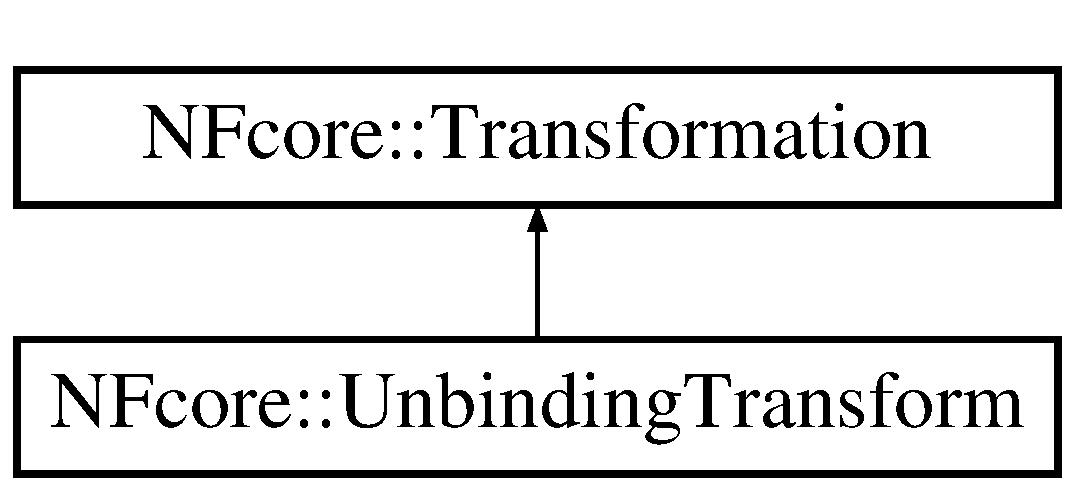
\includegraphics[height=2cm]{classNFcore_1_1UnbindingTransform}
\end{center}
\end{figure}
\subsection*{Public Member Functions}
\begin{CompactItemize}
\item 
{\bf UnbindingTransform} (int {\bf cIndex})
\item 
virtual {\bf $\sim$UnbindingTransform} ()
\item 
virtual void {\bf apply} ({\bf Mapping} $\ast$m, {\bf MappingSet} $\ast$$\ast$ms)
\item 
virtual int {\bf getComponentIndex} () const 
\end{CompactItemize}
\subsection*{Protected Attributes}
\begin{CompactItemize}
\item 
int {\bf cIndex}
\end{CompactItemize}


\subsection{Constructor \& Destructor Documentation}
\index{NFcore::UnbindingTransform@{NFcore::UnbindingTransform}!UnbindingTransform@{UnbindingTransform}}
\index{UnbindingTransform@{UnbindingTransform}!NFcore::UnbindingTransform@{NFcore::UnbindingTransform}}
\subsubsection{\setlength{\rightskip}{0pt plus 5cm}UnbindingTransform::UnbindingTransform (int {\em cIndex})}\label{classNFcore_1_1UnbindingTransform_dcc314d2dcea9944262301e7d8097e3f}


\index{NFcore::UnbindingTransform@{NFcore::UnbindingTransform}!$\sim$UnbindingTransform@{$\sim$UnbindingTransform}}
\index{$\sim$UnbindingTransform@{$\sim$UnbindingTransform}!NFcore::UnbindingTransform@{NFcore::UnbindingTransform}}
\subsubsection{\setlength{\rightskip}{0pt plus 5cm}virtual NFcore::UnbindingTransform::$\sim$UnbindingTransform ()\hspace{0.3cm}{\tt  [inline, virtual]}}\label{classNFcore_1_1UnbindingTransform_a48b210d817a9f2993fadb6881480880}




\subsection{Member Function Documentation}
\index{NFcore::UnbindingTransform@{NFcore::UnbindingTransform}!apply@{apply}}
\index{apply@{apply}!NFcore::UnbindingTransform@{NFcore::UnbindingTransform}}
\subsubsection{\setlength{\rightskip}{0pt plus 5cm}void UnbindingTransform::apply ({\bf Mapping} $\ast$ {\em m}, {\bf MappingSet} $\ast$$\ast$ {\em ms})\hspace{0.3cm}{\tt  [virtual]}}\label{classNFcore_1_1UnbindingTransform_bc0ad11a6deed270f892cc2c072f016d}




Implements {\bf NFcore::Transformation} \doxyref{}{p.}{classNFcore_1_1Transformation_6a57f607676c92b2465427e57bc7fae5}.\index{NFcore::UnbindingTransform@{NFcore::UnbindingTransform}!getComponentIndex@{getComponentIndex}}
\index{getComponentIndex@{getComponentIndex}!NFcore::UnbindingTransform@{NFcore::UnbindingTransform}}
\subsubsection{\setlength{\rightskip}{0pt plus 5cm}virtual int NFcore::UnbindingTransform::getComponentIndex () const\hspace{0.3cm}{\tt  [inline, virtual]}}\label{classNFcore_1_1UnbindingTransform_d0f5ce90812bad1d25a8b3de001f04d7}




Implements {\bf NFcore::Transformation} \doxyref{}{p.}{classNFcore_1_1Transformation_2ba394b20768b21ba328431103474607}.

\subsection{Member Data Documentation}
\index{NFcore::UnbindingTransform@{NFcore::UnbindingTransform}!cIndex@{cIndex}}
\index{cIndex@{cIndex}!NFcore::UnbindingTransform@{NFcore::UnbindingTransform}}
\subsubsection{\setlength{\rightskip}{0pt plus 5cm}int {\bf NFcore::UnbindingTransform::cIndex}\hspace{0.3cm}{\tt  [protected]}}\label{classNFcore_1_1UnbindingTransform_10f7b72aa782a10ed1a3ca842017a4c6}




The documentation for this class was generated from the following files:\begin{CompactItemize}
\item 
/home/msneddon/eclipse/ganymede\_\-cpp/workspace/NFsim\_\-svn/src/NFreactions/transformations/{\bf transformation.hh}\item 
/home/msneddon/eclipse/ganymede\_\-cpp/workspace/NFsim\_\-svn/src/NFreactions/transformations/{\bf transformation.cpp}\end{CompactItemize}

\chapter{NFsim File Documentation}
\section{/home/msneddon/eclipse/indigo/workspace/NFsim/src/NFcore/complex.cpp File Reference}
\label{complex_8cpp}\index{/home/msneddon/eclipse/indigo/workspace/NFsim/src/NFcore/complex.cpp@{/home/msneddon/eclipse/indigo/workspace/NFsim/src/NFcore/complex.cpp}}


{\tt \#include $<$iostream$>$}\par
{\tt \#include \char`\"{}NFcore.hh\char`\"{}}\par
{\tt \#include $<$string$>$}\par
\subsection*{Namespaces}
\begin{CompactItemize}
\item 
namespace {\bf std}
\end{CompactItemize}
\subsection*{Classes}
\begin{CompactItemize}
\item 
class {\bf IsInWrongComplex}
\end{CompactItemize}

\section{/home/msneddon/eclipse/indigo/workspace/NFsim/src/NFcore/molecule.cpp File Reference}
\label{molecule_8cpp}\index{/home/msneddon/eclipse/indigo/workspace/NFsim/src/NFcore/molecule.cpp@{/home/msneddon/eclipse/indigo/workspace/NFsim/src/NFcore/molecule.cpp}}


{\tt \#include $<$iostream$>$}\par
{\tt \#include \char`\"{}NFcore.hh\char`\"{}}\par
{\tt \#include $<$queue$>$}\par

\section{/home/msneddon/eclipse/galileoSR1\_\-cpp/workspace/NFsim/src/NFcore/moleculeLists/moleculeList.cpp File Reference}
\label{moleculeList_8cpp}\index{/home/msneddon/eclipse/galileoSR1\_\-cpp/workspace/NFsim/src/NFcore/moleculeLists/moleculeList.cpp@{/home/msneddon/eclipse/galileoSR1\_\-cpp/workspace/NFsim/src/NFcore/moleculeLists/moleculeList.cpp}}


{\tt \#include \char`\"{}moleculeList.hh\char`\"{}}\par

\section{/home/msneddon/eclipse/ganymede\_\-cpp/workspace/NFsim\_\-svn/src/NFcore/moleculeLists/moleculeList.hh File Reference}
\label{moleculeList_8hh}\index{/home/msneddon/eclipse/ganymede\_\-cpp/workspace/NFsim\_\-svn/src/NFcore/moleculeLists/moleculeList.hh@{/home/msneddon/eclipse/ganymede\_\-cpp/workspace/NFsim\_\-svn/src/NFcore/moleculeLists/moleculeList.hh}}


{\tt \#include \char`\"{}../NFcore.hh\char`\"{}}\par
\subsection*{Namespaces}
\begin{CompactItemize}
\item 
namespace {\bf NFcore}
\end{CompactItemize}
\subsection*{Classes}
\begin{CompactItemize}
\item 
class {\bf NFcore::MoleculeList}
\begin{CompactList}\small\item\em Keeps a set of molecules neatly for a \doxyref{MoleculeType}{p.}{classNFcore_1_1MoleculeType}. \item\end{CompactList}\end{CompactItemize}

\section{/home/msneddon/eclipse/indigo/workspace/NFsim/src/NFcore/moleculeType.cpp File Reference}
\label{moleculeType_8cpp}\index{/home/msneddon/eclipse/indigo/workspace/NFsim/src/NFcore/moleculeType.cpp@{/home/msneddon/eclipse/indigo/workspace/NFsim/src/NFcore/moleculeType.cpp}}


{\tt \#include $<$iostream$>$}\par
{\tt \#include \char`\"{}NFcore.hh\char`\"{}}\par
\subsection*{Functions}
\begin{CompactItemize}
\item 
{\footnotesize template$<$class T$>$ }\\{\bf NFstream} \& {\bf operator$<$$<$} ({\bf NFstream} \&nfstream, const T \&value)
\end{CompactItemize}


\subsection{Function Documentation}
\index{moleculeType.cpp@{moleculeType.cpp}!operator$<$$<$@{operator$<$$<$}}
\index{operator$<$$<$@{operator$<$$<$}!moleculeType.cpp@{moleculeType.cpp}}
\subsubsection{\setlength{\rightskip}{0pt plus 5cm}template$<$class T$>$ {\bf NFstream}\& operator$<$$<$ ({\bf NFstream} \& {\em nfstream}, const T \& {\em value})\hspace{0.3cm}{\tt  [inline]}}\label{moleculeType_8cpp_ef588953052314e1b69285568a59947f}



\section{/home/msneddon/eclipse/galileoSR1\_\-cpp/workspace/NFsim/src/NFcore/NFcore.hh File Reference}
\label{NFcore_8hh}\index{/home/msneddon/eclipse/galileoSR1\_\-cpp/workspace/NFsim/src/NFcore/NFcore.hh@{/home/msneddon/eclipse/galileoSR1\_\-cpp/workspace/NFsim/src/NFcore/NFcore.hh}}


\subsection{Detailed Description}
Contains declarations of core NFsim classes. 



{\tt \#include $<$iostream$>$}\par
{\tt \#include $<$fstream$>$}\par
{\tt \#include $<$string$>$}\par
{\tt \#include $<$vector$>$}\par
{\tt \#include $<$list$>$}\par
{\tt \#include $<$queue$>$}\par
{\tt \#include $<$map$>$}\par
{\tt \#include \char`\"{}../NFscheduler/NFstream.h\char`\"{}}\par
{\tt \#include \char`\"{}../NFutil/NFutil.hh\char`\"{}}\par
{\tt \#include \char`\"{}../NFreactions/NFreactions.hh\char`\"{}}\par
{\tt \#include \char`\"{}moleculeLists/moleculeList.hh\char`\"{}}\par
{\tt \#include \char`\"{}../NFfunction/NFfunction.hh\char`\"{}}\par
{\tt \#include \char`\"{}../NFoutput/NFoutput.hh\char`\"{}}\par
{\tt \#include \char`\"{}reactionSelector/reactionSelector.hh\char`\"{}}\par
{\tt \#include \char`\"{}templateMolecule.hh\char`\"{}}\par
{\tt \#include \char`\"{}observable.hh\char`\"{}}\par
\subsection*{Namespaces}
\begin{CompactItemize}
\item 
namespace {\bf NFcore}
\end{CompactItemize}
\subsection*{Classes}
\begin{CompactItemize}
\item 
class {\bf NFcore::ComplexList}
\begin{CompactList}\small\item\em Container to organize all system complexes. \item\end{CompactList}\item 
class {\bf NFcore::System}
\begin{CompactList}\small\item\em The main class that begins and runs simulations. \item\end{CompactList}\item 
class {\bf NFcore::MoleculeType}
\begin{CompactList}\small\item\em Keeps track of the types of molecules that can exist. \item\end{CompactList}\item 
class {\bf NFcore::Molecule}
\begin{CompactList}\small\item\em Each molecule in the system is represented by an instance of this. \item\end{CompactList}\item 
class {\bf NFcore::ReactionClass}
\begin{CompactList}\small\item\em Abstract Base Class that defines the interface for all reaction rules. \item\end{CompactList}\item 
class {\bf NFcore::Complex}
\begin{CompactList}\small\item\em Container to dynamically keep track of all system complexes. \item\end{CompactList}\end{CompactItemize}
\subsection*{Defines}
\begin{CompactItemize}
\item 
\#define {\bf DEBUG}~0
\item 
\#define {\bf BASIC\_\-MESSAGE}~0
\end{CompactItemize}


\subsection{Define Documentation}
\index{NFcore.hh@{NFcore.hh}!BASIC\_\-MESSAGE@{BASIC\_\-MESSAGE}}
\index{BASIC\_\-MESSAGE@{BASIC\_\-MESSAGE}!NFcore.hh@{NFcore.hh}}
\subsubsection{\setlength{\rightskip}{0pt plus 5cm}\#define BASIC\_\-MESSAGE~0}\label{NFcore_8hh_549c8d787626121534e8783de2a9685e}


\index{NFcore.hh@{NFcore.hh}!DEBUG@{DEBUG}}
\index{DEBUG@{DEBUG}!NFcore.hh@{NFcore.hh}}
\subsubsection{\setlength{\rightskip}{0pt plus 5cm}\#define DEBUG~0}\label{NFcore_8hh_d72dbcf6d0153db1b8d8a58001feed83}



\section{/home/msneddon/eclipse/galileoSR1\_\-cpp/workspace/NFsim/src/NFcore/observable.cpp File Reference}
\label{observable_8cpp}\index{/home/msneddon/eclipse/galileoSR1\_\-cpp/workspace/NFsim/src/NFcore/observable.cpp@{/home/msneddon/eclipse/galileoSR1\_\-cpp/workspace/NFsim/src/NFcore/observable.cpp}}


{\tt \#include $<$iostream$>$}\par
{\tt \#include \char`\"{}observable.hh\char`\"{}}\par

\section{/home/msneddon/eclipse/ganymede\_\-cpp/workspace/NFsim\_\-svn/src/NFcore/reactionClass.cpp File Reference}
\label{reactionClass_8cpp}\index{/home/msneddon/eclipse/ganymede\_\-cpp/workspace/NFsim\_\-svn/src/NFcore/reactionClass.cpp@{/home/msneddon/eclipse/ganymede\_\-cpp/workspace/NFsim\_\-svn/src/NFcore/reactionClass.cpp}}


{\tt \#include \char`\"{}NFcore.hh\char`\"{}}\par

\section{/home/msneddon/eclipse/ganymede\_\-cpp/workspace/NFsim\_\-svn/src/NFcore/system.cpp File Reference}
\label{system_8cpp}\index{/home/msneddon/eclipse/ganymede\_\-cpp/workspace/NFsim\_\-svn/src/NFcore/system.cpp@{/home/msneddon/eclipse/ganymede\_\-cpp/workspace/NFsim\_\-svn/src/NFcore/system.cpp}}


{\tt \#include \char`\"{}NFcore.hh\char`\"{}}\par
{\tt \#include $<$math.h$>$}\par
{\tt \#include $<$fstream$>$}\par

\section{/home/msneddon/eclipse/galileoSR1\_\-cpp/workspace/NFsim/src/NFcore/templateMolecule.cpp File Reference}
\label{templateMolecule_8cpp}\index{/home/msneddon/eclipse/galileoSR1\_\-cpp/workspace/NFsim/src/NFcore/templateMolecule.cpp@{/home/msneddon/eclipse/galileoSR1\_\-cpp/workspace/NFsim/src/NFcore/templateMolecule.cpp}}


{\tt \#include $<$iostream$>$}\par
{\tt \#include \char`\"{}templateMolecule.hh\char`\"{}}\par
\subsection*{Functions}
\begin{CompactItemize}
\item 
string {\bf addStateConstraint} (string original, string compName, string newConstraint)
\item 
string {\bf addBondConstraint} (string original, string compName, int bondNumber)
\end{CompactItemize}


\subsection{Function Documentation}
\index{templateMolecule.cpp@{templateMolecule.cpp}!addBondConstraint@{addBondConstraint}}
\index{addBondConstraint@{addBondConstraint}!templateMolecule.cpp@{templateMolecule.cpp}}
\subsubsection{\setlength{\rightskip}{0pt plus 5cm}string addBondConstraint (string {\em original}, string {\em compName}, int {\em bondNumber})}\label{templateMolecule_8cpp_7cb43d45a2c9b9949241f1351c3ed7b0}


\index{templateMolecule.cpp@{templateMolecule.cpp}!addStateConstraint@{addStateConstraint}}
\index{addStateConstraint@{addStateConstraint}!templateMolecule.cpp@{templateMolecule.cpp}}
\subsubsection{\setlength{\rightskip}{0pt plus 5cm}string addStateConstraint (string {\em original}, string {\em compName}, string {\em newConstraint})}\label{templateMolecule_8cpp_7c45e3f4b9c8d3d06577f5f30f661857}



\section{/home/msneddon/eclipse/ganymede\_\-cpp/workspace/NFsim\_\-svn/src/NFfunction/funcParser.cpp File Reference}
\label{funcParser_8cpp}\index{/home/msneddon/eclipse/ganymede\_\-cpp/workspace/NFsim\_\-svn/src/NFfunction/funcParser.cpp@{/home/msneddon/eclipse/ganymede\_\-cpp/workspace/NFsim\_\-svn/src/NFfunction/funcParser.cpp}}


{\tt \#include \char`\"{}NFfunction.hh\char`\"{}}\par
{\tt \#include $<$math.h$>$}\par
\subsection*{Namespaces}
\begin{CompactItemize}
\item 
namespace {\bf mu}
\end{CompactItemize}

\section{/home/msneddon/eclipse/indigo/workspace/NFsim/src/NFfunction/function.cpp File Reference}
\label{function_8cpp}\index{/home/msneddon/eclipse/indigo/workspace/NFsim/src/NFfunction/function.cpp@{/home/msneddon/eclipse/indigo/workspace/NFsim/src/NFfunction/function.cpp}}


{\tt \#include \char`\"{}NFfunction.hh\char`\"{}}\par

\section{/home/msneddon/eclipse/ganymede\_\-cpp/workspace/NFsim\_\-svn/src/NFfunction/NFfunction.hh File Reference}
\label{NFfunction_8hh}\index{/home/msneddon/eclipse/ganymede\_\-cpp/workspace/NFsim\_\-svn/src/NFfunction/NFfunction.hh@{/home/msneddon/eclipse/ganymede\_\-cpp/workspace/NFsim\_\-svn/src/NFfunction/NFfunction.hh}}


{\tt \#include \char`\"{}muParser/muParser.h\char`\"{}}\par
{\tt \#include \char`\"{}../NFcore/NFcore.hh\char`\"{}}\par
\subsection*{Namespaces}
\begin{CompactItemize}
\item 
namespace {\bf NFcore}
\end{CompactItemize}
\subsection*{Classes}
\begin{CompactItemize}
\item 
class {\bf NFcore::FuncFactory}
\begin{CompactList}\small\item\em Parses mathmatical functions that can be easily used anywhere. \item\end{CompactList}\item 
class {\bf NFcore::GlobalFunction}
\begin{CompactList}\small\item\em Defines functions to be used globally in a simulation. \item\end{CompactList}\item 
class {\bf NFcore::StateCounter}
\item 
class {\bf NFcore::LocalFunction}
\end{CompactItemize}

\section{/home/msneddon/eclipse/galileoSR1\_\-cpp/workspace/NFsim/src/NFinput/commandLineParser.cpp File Reference}
\label{commandLineParser_8cpp}\index{/home/msneddon/eclipse/galileoSR1\_\-cpp/workspace/NFsim/src/NFinput/commandLineParser.cpp@{/home/msneddon/eclipse/galileoSR1\_\-cpp/workspace/NFsim/src/NFinput/commandLineParser.cpp}}


{\tt \#include \char`\"{}NFinput.hh\char`\"{}}\par
\subsection*{Functions}
\begin{CompactItemize}
\item 
bool {\bf NFinput::parseArguments} (int argc, const char $\ast$argv[$\,$], map$<$ string, string $>$ \&argMap)
\begin{CompactList}\small\item\em Parses command line arguments from the console nicely. \item\end{CompactList}\item 
int {\bf NFinput::parseAsInt} (map$<$ string, string $>$ \&argMap, string argName, int defaultValue)
\begin{CompactList}\small\item\em Looks up the argument in the argMap and tries to parse the value as an integer. \item\end{CompactList}\item 
void {\bf NFinput::parseAsCommaSeparatedSequence} (map$<$ string, string $>$ \&argMap, string argName, vector$<$ int $>$ \&sequence)
\begin{CompactList}\small\item\em Looks up the argument in the argMap and tries to parse the value as a comma delimited sequence of ints. \item\end{CompactList}\item 
double {\bf NFinput::parseAsDouble} (map$<$ string, string $>$ \&argMap, string argName, double defaultValue)
\begin{CompactList}\small\item\em Looks up the argument in the argMap and tries to parse the value as a double. \item\end{CompactList}\item 
bool {\bf NFinput::parseSequence} (string numString, vector$<$ double $>$ \&outputTimes)
\begin{CompactList}\small\item\em Parses a matlab style sequence (ie startValue:step:endValue) into the vector. \item\end{CompactList}\item 
bool {\bf NFinput::createSystemDumper} (string paramStr, {\bf System} $\ast$s, bool verbose)
\begin{CompactList}\small\item\em Parses the cmd line arg that specifies system dumps, and schedules them. \item\end{CompactList}\end{CompactItemize}

\section{/home/msneddon/eclipse/galileoSR1\_\-cpp/workspace/NFsim/src/NFinput/NFinput.cpp File Reference}
\label{NFinput_8cpp}\index{/home/msneddon/eclipse/galileoSR1\_\-cpp/workspace/NFsim/src/NFinput/NFinput.cpp@{/home/msneddon/eclipse/galileoSR1\_\-cpp/workspace/NFsim/src/NFinput/NFinput.cpp}}


{\tt \#include \char`\"{}NFinput.hh\char`\"{}}\par
\subsection*{Functions}
\begin{CompactItemize}
\item 
{\bf System} $\ast$ {\bf NFinput::initializeFromXML} (string filename, bool blockSameComplexBinding, int globalMoleculeLimit, bool verbose, int \&suggestedTraversalLimit)
\begin{CompactList}\small\item\em Maintains information about a \doxyref{component}{p.}{classNFinput_1_1component} of a TemplateMolecule. \item\end{CompactList}\item 
bool {\bf NFinput::initParameters} ({\bf TiXmlElement} $\ast$pListOfParameters, {\bf System} $\ast$s, map$<$ string, double $>$ \&parameter, bool verbose)
\begin{CompactList}\small\item\em Reads the parameter XML block and puts them in the parameter map. \item\end{CompactList}\item 
bool {\bf NFinput::initMoleculeTypes} ({\bf TiXmlElement} $\ast$pListOfMoleculeTypes, {\bf System} $\ast$system, map$<$ string, int $>$ \&allowedStates, bool verbose)
\begin{CompactList}\small\item\em Reads the MoleculeType XML block and adds the MoleculeTypes to the system. \item\end{CompactList}\item 
bool {\bf NFinput::initStartSpecies} ({\bf TiXmlElement} $\ast$pListOfSpecies, {\bf System} $\ast$system, map$<$ string, double $>$ \&parameter, map$<$ string, int $>$ \&allowedStates, bool verbose)
\begin{CompactList}\small\item\em Reads a Species XML block, creates the molecules and adds them to the system. \item\end{CompactList}\item 
bool {\bf NFinput::initReactionRules} ({\bf TiXmlElement} $\ast$pListOfReactionRules, {\bf System} $\ast$system, map$<$ string, double $>$ \&parameter, map$<$ string, int $>$ \&allowedStates, bool blockSameComplexBinding, bool verbose, int \&suggestedTraversalLimit)
\begin{CompactList}\small\item\em Reads a reactionRule XML block and adds the rules to the system. \item\end{CompactList}\item 
bool {\bf NFinput::readObservableForTemplateMolecules} ({\bf TiXmlElement} $\ast$pObs, string observableName, vector$<$ {\bf TemplateMolecule} $\ast$ $>$ \&tmList, vector$<$ string $>$ \&stochRelation, vector$<$ int $>$ \&stochQuantity, {\bf System} $\ast$s, map$<$ string, double $>$ \&parameter, map$<$ string, int $>$ \&allowedStates, int obsType, bool verbose, int \&suggestedTraversalLimit)
\item 
bool {\bf NFinput::initObservables} ({\bf TiXmlElement} $\ast$pListOfObservables, {\bf System} $\ast$system, map$<$ string, double $>$ \&parameter, map$<$ string, int $>$ \&allowedStates, bool verbose, int \&suggestedTraversalLimit)
\begin{CompactList}\small\item\em Reads an observable XML block and adds the new observables to the system. \item\end{CompactList}\item 
{\bf TemplateMolecule} $\ast$ {\bf NFinput::readPattern} ({\bf TiXmlElement} $\ast$pListOfMol, {\bf System} $\ast$s, map$<$ string, double $>$ \&parameter, map$<$ string, int $>$ \&allowedStates, string patternName, map$<$ string, {\bf TemplateMolecule} $\ast$ $>$ \&templates, map$<$ string, {\bf component} $>$ \&comps, map$<$ string, {\bf component} $>$ \&symMap, bool verbose, int \&suggestedTraversalLimit)
\begin{CompactList}\small\item\em Reads a pattern XML block and returns the set of new TemplateMolecule objects. \item\end{CompactList}\item 
bool {\bf NFinput::readProductPattern} ({\bf TiXmlElement} $\ast$pListOfMol, {\bf System} $\ast$s, map$<$ string, double $>$ \&parameter, map$<$ string, int $>$ \&allowedStates, string patternName, vector$<$ {\bf MoleculeType} $\ast$ $>$ \&productMoleculeTypes, vector$<$ vector$<$ int $>$ $>$ \&stateInformation, vector$<$ vector$<$ int $>$ $>$ \&bindingSiteInformation, bool verbose)
\begin{CompactList}\small\item\em Reads a pattern XML block and returns the set of new TemplateMolecule objects. \item\end{CompactList}\item 
bool {\bf NFinput::readProductMolecule} ({\bf TiXmlElement} $\ast$pMol, {\bf System} $\ast$s, map$<$ string, double $>$ \&parameter, map$<$ string, int $>$ \&allowedStates, string patternName, vector$<$ {\bf MoleculeCreator} $\ast$ $>$ \&moleculeCreatorsList, map$<$ string, {\bf component} $>$ \&comps, bool verbose)
\begin{CompactList}\small\item\em Reads a product molecule XML block and returns a TemplateMolecule objects. \item\end{CompactList}\end{CompactItemize}

\section{/home/msneddon/eclipse/galileoSR1\_\-cpp/workspace/NFsim/src/NFinput/NFinput.hh File Reference}
\label{NFinput_8hh}\index{/home/msneddon/eclipse/galileoSR1\_\-cpp/workspace/NFsim/src/NFinput/NFinput.hh@{/home/msneddon/eclipse/galileoSR1\_\-cpp/workspace/NFsim/src/NFinput/NFinput.hh}}


{\tt \#include $<$iostream$>$}\par
{\tt \#include $<$map$>$}\par
{\tt \#include $<$vector$>$}\par
{\tt \#include $<$stdio.h$>$}\par
{\tt \#include $<$limits.h$>$}\par
{\tt \#include $<$exception$>$}\par
{\tt \#include \char`\"{}../NFcore/NFcore.hh\char`\"{}}\par
{\tt \#include \char`\"{}../NFoutput/NFoutput.hh\char`\"{}}\par
{\tt \#include \char`\"{}../NFfunction/NFfunction.hh\char`\"{}}\par
{\tt \#include \char`\"{}../NFreactions/reactions/reaction.hh\char`\"{}}\par
{\tt \#include \char`\"{}TinyXML/tinyxml.h\char`\"{}}\par
\subsection*{Namespaces}
\begin{CompactItemize}
\item 
namespace {\bf NFinput}
\end{CompactItemize}
\subsection*{Classes}
\begin{CompactItemize}
\item 
class {\bf NFinput::component}
\begin{CompactList}\small\item\em Maintains information about a \doxyref{component}{p.}{classNFinput_1_1component} of a TemplateMolecule. \item\end{CompactList}\end{CompactItemize}
\subsection*{Functions}
\begin{CompactItemize}
\item 
{\bf System} $\ast$ {\bf NFinput::initializeFromXML} (string filename, bool blockSameComplexBinding, int globalMoleculeLimit, bool verbose)
\begin{CompactList}\small\item\em Maintains information about a \doxyref{component}{p.}{classNFinput_1_1component} of a TemplateMolecule. \item\end{CompactList}\item 
bool {\bf NFinput::initParameters} ({\bf TiXmlElement} $\ast$pListOfParameters, {\bf System} $\ast$s, map$<$ string, double $>$ \&parameter, bool verbose)
\begin{CompactList}\small\item\em Reads the parameter XML block and puts them in the parameter map. \item\end{CompactList}\item 
bool {\bf NFinput::initFunctions} ({\bf TiXmlElement} $\ast$pListOfFunctions, {\bf System} $\ast$system, map$<$ string, double $>$ \&parameter, {\bf TiXmlElement} $\ast$pListOfObservables, map$<$ string, int $>$ \&allowedStates, bool verbose)
\begin{CompactList}\small\item\em Reads the Function XML block and adds the Functions to the system. \item\end{CompactList}\item 
bool {\bf NFinput::initMoleculeTypes} ({\bf TiXmlElement} $\ast$pListOfMoleculeTypes, {\bf System} $\ast$system, map$<$ string, int $>$ \&allowedStates, bool verbose)
\begin{CompactList}\small\item\em Reads the MoleculeType XML block and adds the MoleculeTypes to the system. \item\end{CompactList}\item 
bool {\bf NFinput::FindReactionRuleSymmetry} ({\bf TiXmlElement} $\ast$pRxnRule, {\bf System} $\ast$s, map$<$ string, double $>$ \&parameter, map$<$ string, int $>$ \&allowedStates, map$<$ string, {\bf component} $>$ \&symComps, map$<$ string, {\bf component} $>$ \&symRxnCenter, bool verbose)
\item 
bool {\bf NFinput::readPatternForSymmetry} ({\bf TiXmlElement} $\ast$pListOfMol, {\bf System} $\ast$s, string patternName, map$<$ string, {\bf component} $>$ \&comps, map$<$ string, {\bf component} $>$ \&symComps, bool verbose)
\item 
bool {\bf NFinput::generateRxnPermutations} (vector$<$ map$<$ string, {\bf component} $>$ $>$ \&permutations, map$<$ string, {\bf component} $>$ \&symComps, map$<$ string, {\bf component} $>$ \&symRxnCenter, bool verbose)
\item 
bool {\bf NFinput::readObservableForTemplateMolecules} ({\bf TiXmlElement} $\ast$pObs, string observableName, vector$<$ {\bf TemplateMolecule} $\ast$ $>$ \&tmList, vector$<$ string $>$ \&stochRelation, vector$<$ int $>$ \&stochQuantity, {\bf System} $\ast$s, map$<$ string, double $>$ \&parameter, map$<$ string, int $>$ \&allowedStates, int obsType, bool verbose)
\item 
bool {\bf NFinput::initStartSpecies} ({\bf TiXmlElement} $\ast$pListOfSpecies, {\bf System} $\ast$system, map$<$ string, double $>$ \&parameter, map$<$ string, int $>$ \&allowedStates, bool verbose)
\begin{CompactList}\small\item\em Reads a Species XML block, creates the molecules and adds them to the system. \item\end{CompactList}\item 
bool {\bf NFinput::initReactionRules} ({\bf TiXmlElement} $\ast$pListOfReactionRules, {\bf System} $\ast$system, map$<$ string, double $>$ \&parameter, map$<$ string, int $>$ \&allowedStates, bool blockSameComplexBinding, bool verbose)
\begin{CompactList}\small\item\em Reads a reactionRule XML block and adds the rules to the system. \item\end{CompactList}\item 
bool {\bf NFinput::initObservables} ({\bf TiXmlElement} $\ast$pListOfObservables, {\bf System} $\ast$system, map$<$ string, double $>$ \&parameter, map$<$ string, int $>$ \&allowedStates, bool verbose)
\begin{CompactList}\small\item\em Reads an observable XML block and adds the new observables to the system. \item\end{CompactList}\item 
{\bf TemplateMolecule} $\ast$ {\bf NFinput::readPattern} ({\bf TiXmlElement} $\ast$pListOfMol, {\bf System} $\ast$s, map$<$ string, double $>$ \&parameter, map$<$ string, int $>$ \&allowedStates, string patternName, map$<$ string, {\bf TemplateMolecule} $\ast$ $>$ \&templates, map$<$ string, {\bf component} $>$ \&comps, map$<$ string, {\bf component} $>$ \&symMap, bool verbose)
\begin{CompactList}\small\item\em Reads a pattern XML block and returns the set of new TemplateMolecule objects. \item\end{CompactList}\item 
bool {\bf NFinput::readProductPattern} ({\bf TiXmlElement} $\ast$pListOfMol, {\bf System} $\ast$s, map$<$ string, double $>$ \&parameter, map$<$ string, int $>$ \&allowedStates, string patternName, vector$<$ {\bf MoleculeType} $\ast$ $>$ \&productMoleculeTypes, vector$<$ vector$<$ int $>$ $>$ \&stateInformation, vector$<$ vector$<$ int $>$ $>$ \&bindingSiteInformation, bool verbose)
\begin{CompactList}\small\item\em Reads a pattern XML block and returns the set of new TemplateMolecule objects. \item\end{CompactList}\item 
bool {\bf NFinput::lookup} ({\bf component} $\ast$\&c, string id, map$<$ string, {\bf component} $>$ \&comps, map$<$ string, {\bf component} $>$ \&symMap)
\item 
bool {\bf NFinput::parseArguments} (int argc, const char $\ast$argv[$\,$], map$<$ string, string $>$ \&argMap)
\begin{CompactList}\small\item\em Parses command line arguments from the console nicely. \item\end{CompactList}\item 
int {\bf NFinput::parseAsInt} (map$<$ string, string $>$ \&argMap, string argName, int defaultValue)
\begin{CompactList}\small\item\em Looks up the argument in the argMap and tries to parse the value as an integer. \item\end{CompactList}\item 
double {\bf NFinput::parseAsDouble} (map$<$ string, string $>$ \&argMap, string argName, double defaultValue)
\begin{CompactList}\small\item\em Looks up the argument in the argMap and tries to parse the value as a double. \item\end{CompactList}\item 
void {\bf NFinput::walk} ({\bf System} $\ast$s)
\begin{CompactList}\small\item\em Allows the user to walk through the system with an interactive text-based program. \item\end{CompactList}\item 
bool {\bf NFinput::createSystemDumper} (string paramStr, {\bf System} $\ast$s, bool verbose)
\begin{CompactList}\small\item\em Parses the cmd line arg that specifies system dumps, and schedules them. \item\end{CompactList}\item 
bool {\bf NFinput::parseSequence} (string numString, vector$<$ double $>$ \&outputTimes)
\begin{CompactList}\small\item\em Parses a matlab style sequence (ie startValue:step:endValue) into the vector. \item\end{CompactList}\item 
bool {\bf NFinput::readRNFfile} (map$<$ string, string $>$ \&argMap, vector$<$ string $>$ \&commands, bool verbose)
\item 
bool {\bf NFinput::runRNFcommands} ({\bf System} $\ast$s, map$<$ string, string $>$ \&argMap, vector$<$ string $>$ \&commands, bool verbose)
\end{CompactItemize}

\section{/home/msneddon/eclipse/ganymede\_\-cpp/workspace/NFsim\_\-svn/src/NFinput/TinyXML/tinystr.cpp File Reference}
\label{tinystr_8cpp}\index{/home/msneddon/eclipse/ganymede\_\-cpp/workspace/NFsim\_\-svn/src/NFinput/TinyXML/tinystr.cpp@{/home/msneddon/eclipse/ganymede\_\-cpp/workspace/NFsim\_\-svn/src/NFinput/TinyXML/tinystr.cpp}}


{\tt \#include \char`\"{}tinystr.h\char`\"{}}\par
\subsection*{Functions}
\begin{CompactItemize}
\item 
{\bf TiXmlString} {\bf operator+} (const {\bf TiXmlString} \&a, const {\bf TiXmlString} \&b)
\item 
{\bf TiXmlString} {\bf operator+} (const {\bf TiXmlString} \&a, const char $\ast$b)
\item 
{\bf TiXmlString} {\bf operator+} (const char $\ast$a, const {\bf TiXmlString} \&b)
\end{CompactItemize}


\subsection{Function Documentation}
\index{tinystr.cpp@{tinystr.cpp}!operator+@{operator+}}
\index{operator+@{operator+}!tinystr.cpp@{tinystr.cpp}}
\subsubsection{\setlength{\rightskip}{0pt plus 5cm}{\bf TiXmlString} operator+ (const char $\ast$ {\em a}, const {\bf TiXmlString} \& {\em b})}\label{tinystr_8cpp_c0f2988a051a761664d80de81462fc4d}


\index{tinystr.cpp@{tinystr.cpp}!operator+@{operator+}}
\index{operator+@{operator+}!tinystr.cpp@{tinystr.cpp}}
\subsubsection{\setlength{\rightskip}{0pt plus 5cm}{\bf TiXmlString} operator+ (const {\bf TiXmlString} \& {\em a}, const char $\ast$ {\em b})}\label{tinystr_8cpp_b77ef9617d62643b24e52118db159b7b}


\index{tinystr.cpp@{tinystr.cpp}!operator+@{operator+}}
\index{operator+@{operator+}!tinystr.cpp@{tinystr.cpp}}
\subsubsection{\setlength{\rightskip}{0pt plus 5cm}{\bf TiXmlString} operator+ (const {\bf TiXmlString} \& {\em a}, const {\bf TiXmlString} \& {\em b})}\label{tinystr_8cpp_6ee35bce93b3aaf8a2353471c0dd2d58}



\section{/home/msneddon/eclipse/galileoSR1\_\-cpp/workspace/NFsim/src/NFinput/TinyXML/tinystr.h File Reference}
\label{tinystr_8h}\index{/home/msneddon/eclipse/galileoSR1\_\-cpp/workspace/NFsim/src/NFinput/TinyXML/tinystr.h@{/home/msneddon/eclipse/galileoSR1\_\-cpp/workspace/NFsim/src/NFinput/TinyXML/tinystr.h}}


{\tt \#include $<$assert.h$>$}\par
{\tt \#include $<$string.h$>$}\par
\subsection*{Classes}
\begin{CompactItemize}
\item 
class {\bf TiXmlString}
\item 
struct \textbf{TiXmlString::Rep}
\item 
class {\bf TiXmlOutStream}
\end{CompactItemize}
\subsection*{Defines}
\begin{CompactItemize}
\item 
\#define {\bf TIXML\_\-EXPLICIT}
\end{CompactItemize}
\subsection*{Functions}
\begin{CompactItemize}
\item 
bool {\bf operator==} (const {\bf TiXmlString} \&a, const {\bf TiXmlString} \&b)
\item 
bool {\bf operator$<$} (const {\bf TiXmlString} \&a, const {\bf TiXmlString} \&b)
\item 
bool {\bf operator!=} (const {\bf TiXmlString} \&a, const {\bf TiXmlString} \&b)
\item 
bool {\bf operator$>$} (const {\bf TiXmlString} \&a, const {\bf TiXmlString} \&b)
\item 
bool {\bf operator$<$=} (const {\bf TiXmlString} \&a, const {\bf TiXmlString} \&b)
\item 
bool {\bf operator$>$=} (const {\bf TiXmlString} \&a, const {\bf TiXmlString} \&b)
\item 
bool {\bf operator==} (const {\bf TiXmlString} \&a, const char $\ast$b)
\item 
bool {\bf operator==} (const char $\ast$a, const {\bf TiXmlString} \&b)
\item 
bool {\bf operator!=} (const {\bf TiXmlString} \&a, const char $\ast$b)
\item 
bool {\bf operator!=} (const char $\ast$a, const {\bf TiXmlString} \&b)
\item 
{\bf TiXmlString} {\bf operator+} (const {\bf TiXmlString} \&a, const {\bf TiXmlString} \&b)
\item 
{\bf TiXmlString} {\bf operator+} (const {\bf TiXmlString} \&a, const char $\ast$b)
\item 
{\bf TiXmlString} {\bf operator+} (const char $\ast$a, const {\bf TiXmlString} \&b)
\end{CompactItemize}


\subsection{Define Documentation}
\index{tinystr.h@{tinystr.h}!TIXML\_\-EXPLICIT@{TIXML\_\-EXPLICIT}}
\index{TIXML\_\-EXPLICIT@{TIXML\_\-EXPLICIT}!tinystr.h@{tinystr.h}}
\subsubsection{\setlength{\rightskip}{0pt plus 5cm}\#define TIXML\_\-EXPLICIT}\label{tinystr_8h_e341476cd6b94ee32e3e93110a759581}




\subsection{Function Documentation}
\index{tinystr.h@{tinystr.h}!operator"!=@{operator"!=}}
\index{operator"!=@{operator"!=}!tinystr.h@{tinystr.h}}
\subsubsection{\setlength{\rightskip}{0pt plus 5cm}bool operator!= (const char $\ast$ {\em a}, const {\bf TiXmlString} \& {\em b})\hspace{0.3cm}{\tt  [inline]}}\label{tinystr_8h_a37ff9329e975d8aae82ede2051ad8b8}


\index{tinystr.h@{tinystr.h}!operator"!=@{operator"!=}}
\index{operator"!=@{operator"!=}!tinystr.h@{tinystr.h}}
\subsubsection{\setlength{\rightskip}{0pt plus 5cm}bool operator!= (const {\bf TiXmlString} \& {\em a}, const char $\ast$ {\em b})\hspace{0.3cm}{\tt  [inline]}}\label{tinystr_8h_9deca021bf0c79c97b4b3c4a4579e3a4}


\index{tinystr.h@{tinystr.h}!operator"!=@{operator"!=}}
\index{operator"!=@{operator"!=}!tinystr.h@{tinystr.h}}
\subsubsection{\setlength{\rightskip}{0pt plus 5cm}bool operator!= (const {\bf TiXmlString} \& {\em a}, const {\bf TiXmlString} \& {\em b})\hspace{0.3cm}{\tt  [inline]}}\label{tinystr_8h_d56c73c4b133b623f29fdf9e5240296d}


\index{tinystr.h@{tinystr.h}!operator+@{operator+}}
\index{operator+@{operator+}!tinystr.h@{tinystr.h}}
\subsubsection{\setlength{\rightskip}{0pt plus 5cm}{\bf TiXmlString} operator+ (const char $\ast$ {\em a}, const {\bf TiXmlString} \& {\em b})}\label{tinystr_8h_c0f2988a051a761664d80de81462fc4d}


\index{tinystr.h@{tinystr.h}!operator+@{operator+}}
\index{operator+@{operator+}!tinystr.h@{tinystr.h}}
\subsubsection{\setlength{\rightskip}{0pt plus 5cm}{\bf TiXmlString} operator+ (const {\bf TiXmlString} \& {\em a}, const char $\ast$ {\em b})}\label{tinystr_8h_b77ef9617d62643b24e52118db159b7b}


\index{tinystr.h@{tinystr.h}!operator+@{operator+}}
\index{operator+@{operator+}!tinystr.h@{tinystr.h}}
\subsubsection{\setlength{\rightskip}{0pt plus 5cm}{\bf TiXmlString} operator+ (const {\bf TiXmlString} \& {\em a}, const {\bf TiXmlString} \& {\em b})}\label{tinystr_8h_6ee35bce93b3aaf8a2353471c0dd2d58}


\index{tinystr.h@{tinystr.h}!operator$<$@{operator$<$}}
\index{operator$<$@{operator$<$}!tinystr.h@{tinystr.h}}
\subsubsection{\setlength{\rightskip}{0pt plus 5cm}bool operator$<$ (const {\bf TiXmlString} \& {\em a}, const {\bf TiXmlString} \& {\em b})\hspace{0.3cm}{\tt  [inline]}}\label{tinystr_8h_28e13086a32670328b9f4fac22f09ccb}


\index{tinystr.h@{tinystr.h}!operator$<$=@{operator$<$=}}
\index{operator$<$=@{operator$<$=}!tinystr.h@{tinystr.h}}
\subsubsection{\setlength{\rightskip}{0pt plus 5cm}bool operator$<$= (const {\bf TiXmlString} \& {\em a}, const {\bf TiXmlString} \& {\em b})\hspace{0.3cm}{\tt  [inline]}}\label{tinystr_8h_b7fa4756616605a2697128067b80ffa5}


\index{tinystr.h@{tinystr.h}!operator==@{operator==}}
\index{operator==@{operator==}!tinystr.h@{tinystr.h}}
\subsubsection{\setlength{\rightskip}{0pt plus 5cm}bool operator== (const char $\ast$ {\em a}, const {\bf TiXmlString} \& {\em b})\hspace{0.3cm}{\tt  [inline]}}\label{tinystr_8h_a1ab32fa6995bc5bca0e8c0b305d71a7}


\index{tinystr.h@{tinystr.h}!operator==@{operator==}}
\index{operator==@{operator==}!tinystr.h@{tinystr.h}}
\subsubsection{\setlength{\rightskip}{0pt plus 5cm}bool operator== (const {\bf TiXmlString} \& {\em a}, const char $\ast$ {\em b})\hspace{0.3cm}{\tt  [inline]}}\label{tinystr_8h_ce60487cee20f188d1d8c0f4504549da}


\index{tinystr.h@{tinystr.h}!operator==@{operator==}}
\index{operator==@{operator==}!tinystr.h@{tinystr.h}}
\subsubsection{\setlength{\rightskip}{0pt plus 5cm}bool operator== (const {\bf TiXmlString} \& {\em a}, const {\bf TiXmlString} \& {\em b})\hspace{0.3cm}{\tt  [inline]}}\label{tinystr_8h_b43569e63f57a29dbc7deebfee90f98e}


\index{tinystr.h@{tinystr.h}!operator$>$@{operator$>$}}
\index{operator$>$@{operator$>$}!tinystr.h@{tinystr.h}}
\subsubsection{\setlength{\rightskip}{0pt plus 5cm}bool operator$>$ (const {\bf TiXmlString} \& {\em a}, const {\bf TiXmlString} \& {\em b})\hspace{0.3cm}{\tt  [inline]}}\label{tinystr_8h_1390d728e894f489d3f02cedbaf53e35}


\index{tinystr.h@{tinystr.h}!operator$>$=@{operator$>$=}}
\index{operator$>$=@{operator$>$=}!tinystr.h@{tinystr.h}}
\subsubsection{\setlength{\rightskip}{0pt plus 5cm}bool operator$>$= (const {\bf TiXmlString} \& {\em a}, const {\bf TiXmlString} \& {\em b})\hspace{0.3cm}{\tt  [inline]}}\label{tinystr_8h_d5a4ecbced1596c900ac7d7a51660357}



\section{/home/msneddon/eclipse/indigo/workspace/NFsim/src/NFinput/TinyXML/tinyxml.cpp File Reference}
\label{tinyxml_8cpp}\index{/home/msneddon/eclipse/indigo/workspace/NFsim/src/NFinput/TinyXML/tinyxml.cpp@{/home/msneddon/eclipse/indigo/workspace/NFsim/src/NFinput/TinyXML/tinyxml.cpp}}


{\tt \#include $<$ctype.h$>$}\par
{\tt \#include \char`\"{}tinyxml.h\char`\"{}}\par
\subsection*{Functions}
\begin{CompactItemize}
\item 
FILE $\ast$ {\bf TiXmlFOpen} (const char $\ast$filename, const char $\ast$mode)
\end{CompactItemize}


\subsection{Function Documentation}
\index{tinyxml.cpp@{tinyxml.cpp}!TiXmlFOpen@{TiXmlFOpen}}
\index{TiXmlFOpen@{TiXmlFOpen}!tinyxml.cpp@{tinyxml.cpp}}
\subsubsection{\setlength{\rightskip}{0pt plus 5cm}FILE$\ast$ TiXmlFOpen (const char $\ast$ {\em filename}, const char $\ast$ {\em mode})}\label{tinyxml_8cpp_72fac93bfb73cb50c2bfb3f9c8520557}



\section{/home/msneddon/eclipse/ganymede\_\-cpp/workspace/NFsim\_\-svn/src/NFinput/TinyXML/tinyxml.h File Reference}
\label{tinyxml_8h}\index{/home/msneddon/eclipse/ganymede\_\-cpp/workspace/NFsim\_\-svn/src/NFinput/TinyXML/tinyxml.h@{/home/msneddon/eclipse/ganymede\_\-cpp/workspace/NFsim\_\-svn/src/NFinput/TinyXML/tinyxml.h}}


{\tt \#include $<$ctype.h$>$}\par
{\tt \#include $<$stdio.h$>$}\par
{\tt \#include $<$stdlib.h$>$}\par
{\tt \#include $<$string.h$>$}\par
{\tt \#include $<$assert.h$>$}\par
{\tt \#include \char`\"{}tinystr.h\char`\"{}}\par
\subsection*{Classes}
\begin{CompactItemize}
\item 
struct {\bf TiXmlCursor}
\item 
class {\bf TiXmlVisitor}
\item 
class {\bf TiXmlBase}
\item 
struct \textbf{TiXmlBase::Entity}
\item 
class {\bf TiXmlNode}
\item 
class {\bf TiXmlAttribute}
\item 
class {\bf TiXmlAttributeSet}
\item 
class {\bf TiXmlElement}
\item 
class {\bf TiXmlComment}
\item 
class {\bf TiXmlText}
\item 
class {\bf TiXmlDeclaration}
\item 
class {\bf TiXmlUnknown}
\item 
class {\bf TiXmlDocument}
\item 
class {\bf TiXmlHandle}
\item 
class {\bf TiXmlPrinter}
\end{CompactItemize}
\subsection*{Defines}
\begin{CompactItemize}
\item 
\#define {\bf TIXML\_\-STRING}~{\bf TiXmlString}
\item 
\#define {\bf TIXML\_\-SAFE}
\item 
\#define {\bf TIXML\_\-SSCANF}~sscanf
\end{CompactItemize}
\subsection*{Enumerations}
\begin{CompactItemize}
\item 
enum \{ {\bf TIXML\_\-SUCCESS}, 
{\bf TIXML\_\-NO\_\-ATTRIBUTE}, 
{\bf TIXML\_\-WRONG\_\-TYPE}
 \}
\item 
enum {\bf TiXmlEncoding} \{ {\bf TIXML\_\-ENCODING\_\-UNKNOWN}, 
{\bf TIXML\_\-ENCODING\_\-UTF8}, 
{\bf TIXML\_\-ENCODING\_\-LEGACY}
 \}
\end{CompactItemize}
\subsection*{Variables}
\begin{CompactItemize}
\item 
const int {\bf TIXML\_\-MAJOR\_\-VERSION} = 2
\item 
const int {\bf TIXML\_\-MINOR\_\-VERSION} = 5
\item 
const int {\bf TIXML\_\-PATCH\_\-VERSION} = 3
\item 
const {\bf TiXmlEncoding} {\bf TIXML\_\-DEFAULT\_\-ENCODING} = TIXML\_\-ENCODING\_\-UNKNOWN
\end{CompactItemize}


\subsection{Define Documentation}
\index{tinyxml.h@{tinyxml.h}!TIXML\_\-SAFE@{TIXML\_\-SAFE}}
\index{TIXML\_\-SAFE@{TIXML\_\-SAFE}!tinyxml.h@{tinyxml.h}}
\subsubsection{\setlength{\rightskip}{0pt plus 5cm}\#define TIXML\_\-SAFE}\label{tinyxml_8h_5cdc3f402b6b8788f13a408d2be12e8d}


\index{tinyxml.h@{tinyxml.h}!TIXML\_\-SSCANF@{TIXML\_\-SSCANF}}
\index{TIXML\_\-SSCANF@{TIXML\_\-SSCANF}!tinyxml.h@{tinyxml.h}}
\subsubsection{\setlength{\rightskip}{0pt plus 5cm}\#define TIXML\_\-SSCANF~sscanf}\label{tinyxml_8h_96f54d7c855ad92e705510904a040393}


\index{tinyxml.h@{tinyxml.h}!TIXML\_\-STRING@{TIXML\_\-STRING}}
\index{TIXML\_\-STRING@{TIXML\_\-STRING}!tinyxml.h@{tinyxml.h}}
\subsubsection{\setlength{\rightskip}{0pt plus 5cm}\#define TIXML\_\-STRING~{\bf TiXmlString}}\label{tinyxml_8h_92bada05fd84d9a0c9a5bbe53de26887}




\subsection{Enumeration Type Documentation}
\subsubsection{\setlength{\rightskip}{0pt plus 5cm}anonymous enum}\label{tinyxml_8h_06fc87d81c62e9abb8790b6e5713c55b}


\begin{Desc}
\item[Enumerator: ]\par
\begin{description}
\index{TIXML\_\-SUCCESS@{TIXML\_\-SUCCESS}!tinyxml.h@{tinyxml.h}}\index{tinyxml.h@{tinyxml.h}!TIXML\_\-SUCCESS@{TIXML\_\-SUCCESS}}\item[{\em 
TIXML\_\-SUCCESS\label{tinyxml_8h_06fc87d81c62e9abb8790b6e5713c55ba3e89edb94c177db48c4e29f92d737d9}
}]\index{TIXML\_\-NO\_\-ATTRIBUTE@{TIXML\_\-NO\_\-ATTRIBUTE}!tinyxml.h@{tinyxml.h}}\index{tinyxml.h@{tinyxml.h}!TIXML\_\-NO\_\-ATTRIBUTE@{TIXML\_\-NO\_\-ATTRIBUTE}}\item[{\em 
TIXML\_\-NO\_\-ATTRIBUTE\label{tinyxml_8h_06fc87d81c62e9abb8790b6e5713c55bb5d83b77941b021a657f1223e40dc28d}
}]\index{TIXML\_\-WRONG\_\-TYPE@{TIXML\_\-WRONG\_\-TYPE}!tinyxml.h@{tinyxml.h}}\index{tinyxml.h@{tinyxml.h}!TIXML\_\-WRONG\_\-TYPE@{TIXML\_\-WRONG\_\-TYPE}}\item[{\em 
TIXML\_\-WRONG\_\-TYPE\label{tinyxml_8h_06fc87d81c62e9abb8790b6e5713c55b4444723f0e0f7ba0bc120b172120d479}
}]\end{description}
\end{Desc}

\index{tinyxml.h@{tinyxml.h}!TiXmlEncoding@{TiXmlEncoding}}
\index{TiXmlEncoding@{TiXmlEncoding}!tinyxml.h@{tinyxml.h}}
\subsubsection{\setlength{\rightskip}{0pt plus 5cm}enum {\bf TiXmlEncoding}}\label{tinyxml_8h_88d51847a13ee0f4b4d320d03d2c4d96}


\begin{Desc}
\item[Enumerator: ]\par
\begin{description}
\index{TIXML\_\-ENCODING\_\-UNKNOWN@{TIXML\_\-ENCODING\_\-UNKNOWN}!tinyxml.h@{tinyxml.h}}\index{tinyxml.h@{tinyxml.h}!TIXML\_\-ENCODING\_\-UNKNOWN@{TIXML\_\-ENCODING\_\-UNKNOWN}}\item[{\em 
TIXML\_\-ENCODING\_\-UNKNOWN\label{tinyxml_8h_88d51847a13ee0f4b4d320d03d2c4d964f7cb4a48feb16284f2c1620454b3909}
}]\index{TIXML\_\-ENCODING\_\-UTF8@{TIXML\_\-ENCODING\_\-UTF8}!tinyxml.h@{tinyxml.h}}\index{tinyxml.h@{tinyxml.h}!TIXML\_\-ENCODING\_\-UTF8@{TIXML\_\-ENCODING\_\-UTF8}}\item[{\em 
TIXML\_\-ENCODING\_\-UTF8\label{tinyxml_8h_88d51847a13ee0f4b4d320d03d2c4d96f95195ddd184a603ec46225e87059d0a}
}]\index{TIXML\_\-ENCODING\_\-LEGACY@{TIXML\_\-ENCODING\_\-LEGACY}!tinyxml.h@{tinyxml.h}}\index{tinyxml.h@{tinyxml.h}!TIXML\_\-ENCODING\_\-LEGACY@{TIXML\_\-ENCODING\_\-LEGACY}}\item[{\em 
TIXML\_\-ENCODING\_\-LEGACY\label{tinyxml_8h_88d51847a13ee0f4b4d320d03d2c4d966baf76361e2641bb52e08d8b4be412b1}
}]\end{description}
\end{Desc}



\subsection{Variable Documentation}
\index{tinyxml.h@{tinyxml.h}!TIXML\_\-DEFAULT\_\-ENCODING@{TIXML\_\-DEFAULT\_\-ENCODING}}
\index{TIXML\_\-DEFAULT\_\-ENCODING@{TIXML\_\-DEFAULT\_\-ENCODING}!tinyxml.h@{tinyxml.h}}
\subsubsection{\setlength{\rightskip}{0pt plus 5cm}const {\bf TiXmlEncoding} {\bf TIXML\_\-DEFAULT\_\-ENCODING} = TIXML\_\-ENCODING\_\-UNKNOWN}\label{tinyxml_8h_d5b8b092878e9010d6400cb6c13d4879}


\index{tinyxml.h@{tinyxml.h}!TIXML\_\-MAJOR\_\-VERSION@{TIXML\_\-MAJOR\_\-VERSION}}
\index{TIXML\_\-MAJOR\_\-VERSION@{TIXML\_\-MAJOR\_\-VERSION}!tinyxml.h@{tinyxml.h}}
\subsubsection{\setlength{\rightskip}{0pt plus 5cm}const int {\bf TIXML\_\-MAJOR\_\-VERSION} = 2}\label{tinyxml_8h_3b0c714c9be8a776d5d02c5d80e56f34}


\index{tinyxml.h@{tinyxml.h}!TIXML\_\-MINOR\_\-VERSION@{TIXML\_\-MINOR\_\-VERSION}}
\index{TIXML\_\-MINOR\_\-VERSION@{TIXML\_\-MINOR\_\-VERSION}!tinyxml.h@{tinyxml.h}}
\subsubsection{\setlength{\rightskip}{0pt plus 5cm}const int {\bf TIXML\_\-MINOR\_\-VERSION} = 5}\label{tinyxml_8h_4c9cab500d81e6741e23d5087b029764}


\index{tinyxml.h@{tinyxml.h}!TIXML\_\-PATCH\_\-VERSION@{TIXML\_\-PATCH\_\-VERSION}}
\index{TIXML\_\-PATCH\_\-VERSION@{TIXML\_\-PATCH\_\-VERSION}!tinyxml.h@{tinyxml.h}}
\subsubsection{\setlength{\rightskip}{0pt plus 5cm}const int {\bf TIXML\_\-PATCH\_\-VERSION} = 3}\label{tinyxml_8h_2413aed779b03d5768157b299ff79090}



\section{/home/msneddon/eclipse/ganymede\_\-cpp/workspace/NFsim\_\-svn/src/NFinput/TinyXML/tinyxmlerror.cpp File Reference}
\label{tinyxmlerror_8cpp}\index{/home/msneddon/eclipse/ganymede\_\-cpp/workspace/NFsim\_\-svn/src/NFinput/TinyXML/tinyxmlerror.cpp@{/home/msneddon/eclipse/ganymede\_\-cpp/workspace/NFsim\_\-svn/src/NFinput/TinyXML/tinyxmlerror.cpp}}


{\tt \#include \char`\"{}tinyxml.h\char`\"{}}\par

\section{/home/msneddon/eclipse/indigo/workspace/NFsim/src/NFinput/TinyXML/tinyxmlparser.cpp File Reference}
\label{tinyxmlparser_8cpp}\index{/home/msneddon/eclipse/indigo/workspace/NFsim/src/NFinput/TinyXML/tinyxmlparser.cpp@{/home/msneddon/eclipse/indigo/workspace/NFsim/src/NFinput/TinyXML/tinyxmlparser.cpp}}


{\tt \#include $<$ctype.h$>$}\par
{\tt \#include $<$stddef.h$>$}\par
{\tt \#include \char`\"{}tinyxml.h\char`\"{}}\par
\subsection*{Classes}
\begin{CompactItemize}
\item 
class {\bf TiXmlParsingData}
\end{CompactItemize}
\subsection*{Variables}
\begin{CompactItemize}
\item 
const unsigned char {\bf TIXML\_\-UTF\_\-LEAD\_\-0} = 0xefU
\item 
const unsigned char {\bf TIXML\_\-UTF\_\-LEAD\_\-1} = 0xbbU
\item 
const unsigned char {\bf TIXML\_\-UTF\_\-LEAD\_\-2} = 0xbfU
\end{CompactItemize}


\subsection{Variable Documentation}
\index{tinyxmlparser.cpp@{tinyxmlparser.cpp}!TIXML\_\-UTF\_\-LEAD\_\-0@{TIXML\_\-UTF\_\-LEAD\_\-0}}
\index{TIXML\_\-UTF\_\-LEAD\_\-0@{TIXML\_\-UTF\_\-LEAD\_\-0}!tinyxmlparser.cpp@{tinyxmlparser.cpp}}
\subsubsection{\setlength{\rightskip}{0pt plus 5cm}const unsigned char {\bf TIXML\_\-UTF\_\-LEAD\_\-0} = 0xefU}\label{tinyxmlparser_8cpp_37999e32163e2a3280bc0b8e1999774e}


\index{tinyxmlparser.cpp@{tinyxmlparser.cpp}!TIXML\_\-UTF\_\-LEAD\_\-1@{TIXML\_\-UTF\_\-LEAD\_\-1}}
\index{TIXML\_\-UTF\_\-LEAD\_\-1@{TIXML\_\-UTF\_\-LEAD\_\-1}!tinyxmlparser.cpp@{tinyxmlparser.cpp}}
\subsubsection{\setlength{\rightskip}{0pt plus 5cm}const unsigned char {\bf TIXML\_\-UTF\_\-LEAD\_\-1} = 0xbbU}\label{tinyxmlparser_8cpp_3cda92a178036c812663a7b75c5e04d0}


\index{tinyxmlparser.cpp@{tinyxmlparser.cpp}!TIXML\_\-UTF\_\-LEAD\_\-2@{TIXML\_\-UTF\_\-LEAD\_\-2}}
\index{TIXML\_\-UTF\_\-LEAD\_\-2@{TIXML\_\-UTF\_\-LEAD\_\-2}!tinyxmlparser.cpp@{tinyxmlparser.cpp}}
\subsubsection{\setlength{\rightskip}{0pt plus 5cm}const unsigned char {\bf TIXML\_\-UTF\_\-LEAD\_\-2} = 0xbfU}\label{tinyxmlparser_8cpp_8e36ce25f81f009c066037e937da3a6a}



\section{/home/msneddon/eclipse/indigo/workspace/NFsim/src/NFinput/walk.cpp File Reference}
\label{walk_8cpp}\index{/home/msneddon/eclipse/indigo/workspace/NFsim/src/NFinput/walk.cpp@{/home/msneddon/eclipse/indigo/workspace/NFsim/src/NFinput/walk.cpp}}


{\tt \#include \char`\"{}NFinput.hh\char`\"{}}\par
{\tt \#include $<$iostream$>$}\par
\subsection*{Functions}
\begin{CompactItemize}
\item 
int {\bf enterMainMenuLoop} ({\bf System} $\ast$s)
\item 
void {\bf enterStepLoop} ({\bf System} $\ast$s)
\item 
void {\bf getPrintout} ({\bf System} $\ast$s)
\item 
int {\bf getInput} (int min, int max)
\item 
double {\bf getInput} (double min)
\item 
void {\bf NFinput::walk} ({\bf System} $\ast$s)
\begin{CompactList}\small\item\em Allows the user to walk through the system with an interactive text-based program. \item\end{CompactList}\item 
void {\bf printMainMenu} ()
\item 
void {\bf printStepMenu} ()
\item 
void {\bf printSpecificMolecule} ({\bf System} $\ast$s)
\item 
void {\bf printSpecificMoleculeByUid} ({\bf System} $\ast$s)
\end{CompactItemize}


\subsection{Function Documentation}
\index{walk.cpp@{walk.cpp}!enterMainMenuLoop@{enterMainMenuLoop}}
\index{enterMainMenuLoop@{enterMainMenuLoop}!walk.cpp@{walk.cpp}}
\subsubsection{\setlength{\rightskip}{0pt plus 5cm}int enterMainMenuLoop ({\bf System} $\ast$ {\em s})}\label{walk_8cpp_863793acef9098334f0848f1248f1751}


\index{walk.cpp@{walk.cpp}!enterStepLoop@{enterStepLoop}}
\index{enterStepLoop@{enterStepLoop}!walk.cpp@{walk.cpp}}
\subsubsection{\setlength{\rightskip}{0pt plus 5cm}void enterStepLoop ({\bf System} $\ast$ {\em s})}\label{walk_8cpp_35a4c698d1d73333558180211d50f759}


\index{walk.cpp@{walk.cpp}!getInput@{getInput}}
\index{getInput@{getInput}!walk.cpp@{walk.cpp}}
\subsubsection{\setlength{\rightskip}{0pt plus 5cm}double getInput (double {\em min})}\label{walk_8cpp_0e4d21bd159e98d4aba6d9e863e47eb0}


\index{walk.cpp@{walk.cpp}!getInput@{getInput}}
\index{getInput@{getInput}!walk.cpp@{walk.cpp}}
\subsubsection{\setlength{\rightskip}{0pt plus 5cm}int getInput (int {\em min}, int {\em max})}\label{walk_8cpp_bebe2292d72565c713aad9a3bb8bd05f}


\index{walk.cpp@{walk.cpp}!getPrintout@{getPrintout}}
\index{getPrintout@{getPrintout}!walk.cpp@{walk.cpp}}
\subsubsection{\setlength{\rightskip}{0pt plus 5cm}void getPrintout ({\bf System} $\ast$ {\em s})}\label{walk_8cpp_811e5dd97f0e03d876f15766ccd695b0}


\index{walk.cpp@{walk.cpp}!printMainMenu@{printMainMenu}}
\index{printMainMenu@{printMainMenu}!walk.cpp@{walk.cpp}}
\subsubsection{\setlength{\rightskip}{0pt plus 5cm}void printMainMenu ()}\label{walk_8cpp_f9dce1973196a5934ee5ec20ea417324}


\index{walk.cpp@{walk.cpp}!printSpecificMolecule@{printSpecificMolecule}}
\index{printSpecificMolecule@{printSpecificMolecule}!walk.cpp@{walk.cpp}}
\subsubsection{\setlength{\rightskip}{0pt plus 5cm}void printSpecificMolecule ({\bf System} $\ast$ {\em s})}\label{walk_8cpp_3196afa3a219099769f3e53c4bb4a6ea}


\index{walk.cpp@{walk.cpp}!printSpecificMoleculeByUid@{printSpecificMoleculeByUid}}
\index{printSpecificMoleculeByUid@{printSpecificMoleculeByUid}!walk.cpp@{walk.cpp}}
\subsubsection{\setlength{\rightskip}{0pt plus 5cm}void printSpecificMoleculeByUid ({\bf System} $\ast$ {\em s})}\label{walk_8cpp_62848a862d0ba04cd8c21032bf72848b}


\index{walk.cpp@{walk.cpp}!printStepMenu@{printStepMenu}}
\index{printStepMenu@{printStepMenu}!walk.cpp@{walk.cpp}}
\subsubsection{\setlength{\rightskip}{0pt plus 5cm}void printStepMenu ()}\label{walk_8cpp_b199d61dc0e14fa69066c44e274cfd11}



\section{/home/msneddon/eclipse/ganymede\_\-cpp/workspace/NFsim\_\-svn/src/NFoutput/NFoutput.cpp File Reference}
\label{NFoutput_8cpp}\index{/home/msneddon/eclipse/ganymede\_\-cpp/workspace/NFsim\_\-svn/src/NFoutput/NFoutput.cpp@{/home/msneddon/eclipse/ganymede\_\-cpp/workspace/NFsim\_\-svn/src/NFoutput/NFoutput.cpp}}


{\tt \#include \char`\"{}NFoutput.hh\char`\"{}}\par
{\tt \#include $<$queue$>$}\par
{\tt \#include $<$list$>$}\par
\subsection*{Functions}
\begin{CompactItemize}
\item 
void {\bf breadthFirstSearchSeqStyle} (list$<$ {\bf Molecule} $\ast$ $>$ \&members, {\bf Molecule} $\ast$m)
\end{CompactItemize}


\subsection{Function Documentation}
\index{NFoutput.cpp@{NFoutput.cpp}!breadthFirstSearchSeqStyle@{breadthFirstSearchSeqStyle}}
\index{breadthFirstSearchSeqStyle@{breadthFirstSearchSeqStyle}!NFoutput.cpp@{NFoutput.cpp}}
\subsubsection{\setlength{\rightskip}{0pt plus 5cm}void breadthFirstSearchSeqStyle (list$<$ {\bf Molecule} $\ast$ $>$ \& {\em members}, {\bf Molecule} $\ast$ {\em m})}\label{NFoutput_8cpp_7ceb827234c431e04430e7234c7dfe5c}



\section{/home/msneddon/eclipse/galileoSR1\_\-cpp/workspace/NFsim/src/NFoutput/NFoutput.hh File Reference}
\label{NFoutput_8hh}\index{/home/msneddon/eclipse/galileoSR1\_\-cpp/workspace/NFsim/src/NFoutput/NFoutput.hh@{/home/msneddon/eclipse/galileoSR1\_\-cpp/workspace/NFsim/src/NFoutput/NFoutput.hh}}


{\tt \#include \char`\"{}../NFcore/NFcore.hh\char`\"{}}\par
{\tt \#include \char`\"{}../NFutil/NFutil.hh\char`\"{}}\par
\subsection*{Namespaces}
\begin{CompactItemize}
\item 
namespace {\bf NFcore}
\end{CompactItemize}
\subsection*{Classes}
\begin{CompactItemize}
\item 
class {\bf NFcore::Outputter}
\item 
class {\bf NFcore::DumpSystem}
\begin{CompactList}\small\item\em Class for outputting the state of the system. \item\end{CompactList}\end{CompactItemize}

\section{/home/msneddon/eclipse/galileoSR1\_\-cpp/workspace/NFsim/src/NFreactions/mappings/mapping.cpp File Reference}
\label{mapping_8cpp}\index{/home/msneddon/eclipse/galileoSR1\_\-cpp/workspace/NFsim/src/NFreactions/mappings/mapping.cpp@{/home/msneddon/eclipse/galileoSR1\_\-cpp/workspace/NFsim/src/NFreactions/mappings/mapping.cpp}}


{\tt \#include \char`\"{}mapping.hh\char`\"{}}\par

\section{/home/msneddon/eclipse/indigo/workspace/NFsim/src/NFreactions/mappings/mapping.hh File Reference}
\label{mapping_8hh}\index{/home/msneddon/eclipse/indigo/workspace/NFsim/src/NFreactions/mappings/mapping.hh@{/home/msneddon/eclipse/indigo/workspace/NFsim/src/NFreactions/mappings/mapping.hh}}


{\tt \#include \char`\"{}../NFreactions.hh\char`\"{}}\par
{\tt \#include \char`\"{}../NFreactions.hh\char`\"{}}\par
\subsection*{Namespaces}
\begin{CompactItemize}
\item 
namespace {\bf NFcore}
\end{CompactItemize}
\subsection*{Classes}
\begin{CompactItemize}
\item 
class {\bf NFcore::Mapping}
\begin{CompactList}\small\item\em Keeps a pointer to a molecule and remembers a single component to act on. \item\end{CompactList}\end{CompactItemize}

\section{/home/msneddon/eclipse/indigo/workspace/NFsim/src/NFreactions/mappings/mappingGenerator.cpp File Reference}
\label{mappingGenerator_8cpp}\index{/home/msneddon/eclipse/indigo/workspace/NFsim/src/NFreactions/mappings/mappingGenerator.cpp@{/home/msneddon/eclipse/indigo/workspace/NFsim/src/NFreactions/mappings/mappingGenerator.cpp}}


{\tt \#include \char`\"{}mappingGenerator.hh\char`\"{}}\par

\section{/home/msneddon/eclipse/indigo/workspace/NFsim/src/NFreactions/mappings/mappingGenerator.hh File Reference}
\label{mappingGenerator_8hh}\index{/home/msneddon/eclipse/indigo/workspace/NFsim/src/NFreactions/mappings/mappingGenerator.hh@{/home/msneddon/eclipse/indigo/workspace/NFsim/src/NFreactions/mappings/mappingGenerator.hh}}


{\tt \#include \char`\"{}../NFreactions.hh\char`\"{}}\par
{\tt \#include \char`\"{}../NFreactions.hh\char`\"{}}\par
\subsection*{Namespaces}
\begin{CompactItemize}
\item 
namespace {\bf NFcore}
\end{CompactItemize}
\subsection*{Classes}
\begin{CompactItemize}
\item 
class {\bf NFcore::MapGenerator}
\begin{CompactList}\small\item\em Knows how to assign mappings in a \doxyref{MappingSet}{p.}{classNFcore_1_1MappingSet} to a particular \doxyref{Molecule}{p.}{classNFcore_1_1Molecule}. \item\end{CompactList}\end{CompactItemize}

\section{/home/msneddon/eclipse/galileoSR1\_\-cpp/workspace/NFsim/src/NFreactions/mappings/mappingSet.cpp File Reference}
\label{mappingSet_8cpp}\index{/home/msneddon/eclipse/galileoSR1\_\-cpp/workspace/NFsim/src/NFreactions/mappings/mappingSet.cpp@{/home/msneddon/eclipse/galileoSR1\_\-cpp/workspace/NFsim/src/NFreactions/mappings/mappingSet.cpp}}


{\tt \#include \char`\"{}mappingSet.hh\char`\"{}}\par

\section{/home/msneddon/eclipse/ganymede\_\-cpp/workspace/NFsim\_\-svn/src/NFreactions/mappings/mappingSet.hh File Reference}
\label{mappingSet_8hh}\index{/home/msneddon/eclipse/ganymede\_\-cpp/workspace/NFsim\_\-svn/src/NFreactions/mappings/mappingSet.hh@{/home/msneddon/eclipse/ganymede\_\-cpp/workspace/NFsim\_\-svn/src/NFreactions/mappings/mappingSet.hh}}


{\tt \#include \char`\"{}../NFreactions.hh\char`\"{}}\par
{\tt \#include \char`\"{}../NFreactions.hh\char`\"{}}\par
\subsection*{Namespaces}
\begin{CompactItemize}
\item 
namespace {\bf NFcore}
\end{CompactItemize}
\subsection*{Classes}
\begin{CompactItemize}
\item 
class {\bf NFcore::MappingSet}
\begin{CompactList}\small\item\em Keeps a list of mappings needed by a particular list of reactants. \item\end{CompactList}\end{CompactItemize}

\section{/home/msneddon/eclipse/indigo/workspace/NFsim/src/NFreactions/NFreactions.cpp File Reference}
\label{NFreactions_8cpp}\index{/home/msneddon/eclipse/indigo/workspace/NFsim/src/NFreactions/NFreactions.cpp@{/home/msneddon/eclipse/indigo/workspace/NFsim/src/NFreactions/NFreactions.cpp}}


{\tt \#include \char`\"{}NFreactions.hh\char`\"{}}\par
\subsection*{Functions}
\begin{CompactItemize}
\item 
void {\bf NFcore::test} ()
\item 
void {\bf NFcore::test\_\-tree} ()
\item 
void {\bf NFcore::test\_\-simple} ()
\end{CompactItemize}

\section{/home/msneddon/eclipse/galileoSR1\_\-cpp/workspace/NFsim/src/NFreactions/NFreactions.hh File Reference}
\label{NFreactions_8hh}\index{/home/msneddon/eclipse/galileoSR1\_\-cpp/workspace/NFsim/src/NFreactions/NFreactions.hh@{/home/msneddon/eclipse/galileoSR1\_\-cpp/workspace/NFsim/src/NFreactions/NFreactions.hh}}


{\tt \#include $<$vector$>$}\par
{\tt \#include $<$string$>$}\par
{\tt \#include \char`\"{}../NFcore/NFcore.hh\char`\"{}}\par
{\tt \#include \char`\"{}reactantLists/reactantContainer.hh\char`\"{}}\par
{\tt \#include \char`\"{}reactantLists/reactantList.hh\char`\"{}}\par
{\tt \#include \char`\"{}reactantLists/reactantTree.hh\char`\"{}}\par
{\tt \#include \char`\"{}transformations/transformationSet.hh\char`\"{}}\par
{\tt \#include \char`\"{}transformations/transformation.hh\char`\"{}}\par
{\tt \#include \char`\"{}transformations/moleculeCreator.hh\char`\"{}}\par
{\tt \#include \char`\"{}transformations/speciesCreator.hh\char`\"{}}\par
{\tt \#include \char`\"{}mappings/mapping.hh\char`\"{}}\par
{\tt \#include \char`\"{}mappings/mappingSet.hh\char`\"{}}\par
{\tt \#include \char`\"{}mappings/mappingGenerator.hh\char`\"{}}\par
\subsection*{Namespaces}
\begin{CompactItemize}
\item 
namespace {\bf NFcore}
\end{CompactItemize}
\subsection*{Functions}
\begin{CompactItemize}
\item 
void {\bf NFcore::test} ()
\item 
void {\bf NFcore::test\_\-simple} ()
\item 
void {\bf NFcore::test\_\-tree} ()
\end{CompactItemize}

\section{/home/msneddon/eclipse/indigo/workspace/NFsim/src/NFreactions/reactantLists/reactantList.cpp File Reference}
\label{reactantList_8cpp}\index{/home/msneddon/eclipse/indigo/workspace/NFsim/src/NFreactions/reactantLists/reactantList.cpp@{/home/msneddon/eclipse/indigo/workspace/NFsim/src/NFreactions/reactantLists/reactantList.cpp}}


{\tt \#include \char`\"{}reactantList.hh\char`\"{}}\par

\section{/home/msneddon/eclipse/galileoSR1\_\-cpp/workspace/NFsim/src/NFreactions/reactantLists/reactantList.hh File Reference}
\label{reactantList_8hh}\index{/home/msneddon/eclipse/galileoSR1\_\-cpp/workspace/NFsim/src/NFreactions/reactantLists/reactantList.hh@{/home/msneddon/eclipse/galileoSR1\_\-cpp/workspace/NFsim/src/NFreactions/reactantLists/reactantList.hh}}


{\tt \#include \char`\"{}../NFreactions.hh\char`\"{}}\par
{\tt \#include \char`\"{}../NFreactions.hh\char`\"{}}\par
\subsection*{Namespaces}
\begin{CompactItemize}
\item 
namespace {\bf NFcore}
\end{CompactItemize}
\subsection*{Classes}
\begin{CompactItemize}
\item 
class {\bf NFcore::ReactantList}
\begin{CompactList}\small\item\em Maintains a list of MappingSets needed by \doxyref{ReactionClass}{p.}{classNFcore_1_1ReactionClass}. \item\end{CompactList}\end{CompactItemize}

\section{/home/msneddon/eclipse/indigo/workspace/NFsim/src/NFreactions/reactantLists/reactantTree.cpp File Reference}
\label{reactantTree_8cpp}\index{/home/msneddon/eclipse/indigo/workspace/NFsim/src/NFreactions/reactantLists/reactantTree.cpp@{/home/msneddon/eclipse/indigo/workspace/NFsim/src/NFreactions/reactantLists/reactantTree.cpp}}


{\tt \#include \char`\"{}reactantTree.hh\char`\"{}}\par
{\tt \#include $<$math.h$>$}\par
\subsection*{Defines}
\begin{CompactItemize}
\item 
\#define {\bf DEBUG\_\-MESSAGE}~0
\end{CompactItemize}


\subsection{Define Documentation}
\index{reactantTree.cpp@{reactantTree.cpp}!DEBUG\_\-MESSAGE@{DEBUG\_\-MESSAGE}}
\index{DEBUG\_\-MESSAGE@{DEBUG\_\-MESSAGE}!reactantTree.cpp@{reactantTree.cpp}}
\subsubsection{\setlength{\rightskip}{0pt plus 5cm}\#define DEBUG\_\-MESSAGE~0}\label{reactantTree_8cpp_e8523807c48236b849d94507b9eae38f}



\section{/home/msneddon/eclipse/galileoSR1\_\-cpp/workspace/NFsim/src/NFreactions/reactantLists/reactantTree.hh File Reference}
\label{reactantTree_8hh}\index{/home/msneddon/eclipse/galileoSR1\_\-cpp/workspace/NFsim/src/NFreactions/reactantLists/reactantTree.hh@{/home/msneddon/eclipse/galileoSR1\_\-cpp/workspace/NFsim/src/NFreactions/reactantLists/reactantTree.hh}}


{\tt \#include \char`\"{}../NFreactions.hh\char`\"{}}\par
{\tt \#include \char`\"{}../NFreactions.hh\char`\"{}}\par
\subsection*{Namespaces}
\begin{CompactItemize}
\item 
namespace {\bf NFcore}
\end{CompactItemize}
\subsection*{Classes}
\begin{CompactItemize}
\item 
class {\bf NFcore::ReactantTree}
\begin{CompactList}\small\item\em Maintains a tree of MappingSets needed by Distribution of Rates Reactions. \item\end{CompactList}\end{CompactItemize}

\section{/home/msneddon/eclipse/galileoSR1\_\-cpp/workspace/NFsim/src/NFreactions/reactions/DORreaction.cpp File Reference}
\label{DORreaction_8cpp}\index{/home/msneddon/eclipse/galileoSR1\_\-cpp/workspace/NFsim/src/NFreactions/reactions/DORreaction.cpp@{/home/msneddon/eclipse/galileoSR1\_\-cpp/workspace/NFsim/src/NFreactions/reactions/DORreaction.cpp}}


{\tt \#include \char`\"{}reaction.hh\char`\"{}}\par
\subsection*{Defines}
\begin{CompactItemize}
\item 
\#define {\bf DEBUG\_\-MESSAGE}~0
\end{CompactItemize}


\subsection{Define Documentation}
\index{DORreaction.cpp@{DORreaction.cpp}!DEBUG\_\-MESSAGE@{DEBUG\_\-MESSAGE}}
\index{DEBUG\_\-MESSAGE@{DEBUG\_\-MESSAGE}!DORreaction.cpp@{DORreaction.cpp}}
\subsubsection{\setlength{\rightskip}{0pt plus 5cm}\#define DEBUG\_\-MESSAGE~0}\label{DORreaction_8cpp_e8523807c48236b849d94507b9eae38f}



\section{/home/msneddon/eclipse/indigo/workspace/NFsim/src/NFreactions/reactions/reaction.cpp File Reference}
\label{reaction_8cpp}\index{/home/msneddon/eclipse/indigo/workspace/NFsim/src/NFreactions/reactions/reaction.cpp@{/home/msneddon/eclipse/indigo/workspace/NFsim/src/NFreactions/reactions/reaction.cpp}}


{\tt \#include \char`\"{}reaction.hh\char`\"{}}\par

\section{/home/msneddon/eclipse/ganymede\_\-cpp/workspace/NFsim\_\-svn/src/NFreactions/reactions/reaction.hh File Reference}
\label{reaction_8hh}\index{/home/msneddon/eclipse/ganymede\_\-cpp/workspace/NFsim\_\-svn/src/NFreactions/reactions/reaction.hh@{/home/msneddon/eclipse/ganymede\_\-cpp/workspace/NFsim\_\-svn/src/NFreactions/reactions/reaction.hh}}


{\tt \#include \char`\"{}../NFreactions.hh\char`\"{}}\par
\subsection*{Namespaces}
\begin{CompactItemize}
\item 
namespace {\bf NFcore}
\end{CompactItemize}
\subsection*{Classes}
\begin{CompactItemize}
\item 
class {\bf NFcore::BasicRxnClass}
\item 
class {\bf NFcore::FunctionalRxnClass}
\item 
class {\bf NFcore::MMRxnClass}
\item 
class {\bf NFcore::DORRxnClass}
\end{CompactItemize}

\section{/home/msneddon/eclipse/galileoSR1\_\-cpp/workspace/NFsim/src/NFreactions/transformations/speciesCreator.cpp File Reference}
\label{speciesCreator_8cpp}\index{/home/msneddon/eclipse/galileoSR1\_\-cpp/workspace/NFsim/src/NFreactions/transformations/speciesCreator.cpp@{/home/msneddon/eclipse/galileoSR1\_\-cpp/workspace/NFsim/src/NFreactions/transformations/speciesCreator.cpp}}


{\tt \#include \char`\"{}speciesCreator.hh\char`\"{}}\par

\section{/home/msneddon/eclipse/ganymede\_\-cpp/workspace/NFsim\_\-svn/src/NFreactions/transformations/speciesCreator.hh File Reference}
\label{speciesCreator_8hh}\index{/home/msneddon/eclipse/ganymede\_\-cpp/workspace/NFsim\_\-svn/src/NFreactions/transformations/speciesCreator.hh@{/home/msneddon/eclipse/ganymede\_\-cpp/workspace/NFsim\_\-svn/src/NFreactions/transformations/speciesCreator.hh}}


{\tt \#include \char`\"{}../NFreactions.hh\char`\"{}}\par
{\tt \#include \char`\"{}../NFreactions.hh\char`\"{}}\par
\subsection*{Namespaces}
\begin{CompactItemize}
\item 
namespace {\bf NFcore}
\end{CompactItemize}
\subsection*{Classes}
\begin{CompactItemize}
\item 
class {\bf NFcore::SpeciesCreator}
\end{CompactItemize}

\section{/home/msneddon/eclipse/ganymede\_\-cpp/workspace/NFsim\_\-svn/src/NFreactions/transformations/transformation.cpp File Reference}
\label{transformation_8cpp}\index{/home/msneddon/eclipse/ganymede\_\-cpp/workspace/NFsim\_\-svn/src/NFreactions/transformations/transformation.cpp@{/home/msneddon/eclipse/ganymede\_\-cpp/workspace/NFsim\_\-svn/src/NFreactions/transformations/transformation.cpp}}


{\tt \#include \char`\"{}transformation.hh\char`\"{}}\par

\section{/home/msneddon/eclipse/ganymede\_\-cpp/workspace/NFsim\_\-svn/src/NFreactions/transformations/transformation.hh File Reference}
\label{transformation_8hh}\index{/home/msneddon/eclipse/ganymede\_\-cpp/workspace/NFsim\_\-svn/src/NFreactions/transformations/transformation.hh@{/home/msneddon/eclipse/ganymede\_\-cpp/workspace/NFsim\_\-svn/src/NFreactions/transformations/transformation.hh}}


{\tt \#include \char`\"{}../NFreactions.hh\char`\"{}}\par
{\tt \#include \char`\"{}../NFreactions.hh\char`\"{}}\par
\subsection*{Namespaces}
\begin{CompactItemize}
\item 
namespace {\bf NFcore}
\end{CompactItemize}
\subsection*{Classes}
\begin{CompactItemize}
\item 
class {\bf NFcore::TransformationFactory}
\item 
class {\bf NFcore::Transformation}
\item 
class {\bf NFcore::LocalFunctionReference}
\item 
class {\bf NFcore::EmptyTransform}
\item 
class {\bf NFcore::StateChangeTransform}
\item 
class {\bf NFcore::BindingTransform}
\item 
class {\bf NFcore::BindingSeparateComplexTransform}
\item 
class {\bf NFcore::UnbindingTransform}
\item 
class {\bf NFcore::AddMoleculeTransform}
\item 
class {\bf NFcore::RemoveMoleculeTransform}
\item 
class {\bf NFcore::IncrementStateTransform}
\item 
class {\bf NFcore::DecrementStateTransform}
\end{CompactItemize}

\section{/home/msneddon/eclipse/ganymede\_\-cpp/workspace/NFsim\_\-svn/src/NFreactions/transformations/transformationSet.cpp File Reference}
\label{transformationSet_8cpp}\index{/home/msneddon/eclipse/ganymede\_\-cpp/workspace/NFsim\_\-svn/src/NFreactions/transformations/transformationSet.cpp@{/home/msneddon/eclipse/ganymede\_\-cpp/workspace/NFsim\_\-svn/src/NFreactions/transformations/transformationSet.cpp}}


{\tt \#include \char`\"{}transformationSet.hh\char`\"{}}\par

\section{/home/msneddon/eclipse/ganymede\_\-cpp/workspace/NFsim\_\-svn/src/NFreactions/transformations/transformationSet.hh File Reference}
\label{transformationSet_8hh}\index{/home/msneddon/eclipse/ganymede\_\-cpp/workspace/NFsim\_\-svn/src/NFreactions/transformations/transformationSet.hh@{/home/msneddon/eclipse/ganymede\_\-cpp/workspace/NFsim\_\-svn/src/NFreactions/transformations/transformationSet.hh}}


{\tt \#include \char`\"{}../NFreactions.hh\char`\"{}}\par
{\tt \#include \char`\"{}../NFreactions.hh\char`\"{}}\par
\subsection*{Namespaces}
\begin{CompactItemize}
\item 
namespace {\bf NFcore}
\end{CompactItemize}
\subsection*{Classes}
\begin{CompactItemize}
\item 
class {\bf NFcore::TransformationSet}
\begin{CompactList}\small\item\em Maintains a set of \doxyref{Transformation}{p.}{classNFcore_1_1Transformation} objects for a \doxyref{ReactionClass}{p.}{classNFcore_1_1ReactionClass}. \item\end{CompactList}\end{CompactItemize}

\section{/home/msneddon/eclipse/indigo/workspace/NFsim/src/NFsim.cpp File Reference}
\label{NFsim_8cpp}\index{/home/msneddon/eclipse/indigo/workspace/NFsim/src/NFsim.cpp@{/home/msneddon/eclipse/indigo/workspace/NFsim/src/NFsim.cpp}}


{\tt \#include \char`\"{}NFsim.hh\char`\"{}}\par
{\tt \#include $<$iostream$>$}\par
{\tt \#include $<$string$>$}\par
{\tt \#include $<$time.h$>$}\par
{\tt \#include $<$limits$>$}\par
\subsection*{Functions}
\begin{CompactItemize}
\item 
void {\bf printLogo} (int indent, string version)
\begin{CompactList}\small\item\em Outputs an Ascii NFsim logo. \item\end{CompactList}\item 
void {\bf printHelp} (string version)
\begin{CompactList}\small\item\em Outputs a friendly help message. \item\end{CompactList}\item 
bool {\bf runRNFscript} (map$<$ string, string $>$ argMap, bool verbose)
\begin{CompactList}\small\item\em Executes an RNF script from the command line arguments. \item\end{CompactList}\item 
{\bf System} $\ast$ {\bf initSystemFromFlags} (map$<$ string, string $>$ argMap, bool verbose)
\begin{CompactList}\small\item\em Initializes a System object from the arguments. \item\end{CompactList}\item 
int {\bf main} (int argc, char $\ast$argv[$\,$])
\begin{CompactList}\small\item\em Main executable for the NFsim program. \item\end{CompactList}\item 
bool {\bf runFromArgs} ({\bf System} $\ast$s, map$<$ string, string $>$ argMap, bool verbose)
\begin{CompactList}\small\item\em Runs a given System with the specified arguments. \item\end{CompactList}\end{CompactItemize}


\subsection{Function Documentation}
\index{NFsim.cpp@{NFsim.cpp}!initSystemFromFlags@{initSystemFromFlags}}
\index{initSystemFromFlags@{initSystemFromFlags}!NFsim.cpp@{NFsim.cpp}}
\subsubsection{\setlength{\rightskip}{0pt plus 5cm}{\bf System} $\ast$ initSystemFromFlags (map$<$ string, string $>$ {\em argMap}, bool {\em verbose})}\label{NFsim_8cpp_ba72a46366f8d33295a853f07c43a288}


Initializes a System object from the arguments. 

\begin{Desc}
\item[Author:]Michael Sneddon \end{Desc}
\index{NFsim.cpp@{NFsim.cpp}!main@{main}}
\index{main@{main}!NFsim.cpp@{NFsim.cpp}}
\subsubsection{\setlength{\rightskip}{0pt plus 5cm}int main (int {\em argc}, char $\ast$ {\em argv}[$\,$])}\label{NFsim_8cpp_0ddf1224851353fc92bfbff6f499fa97}


Main executable for the NFsim program. 

\begin{Desc}
\item[Author:]Michael Sneddon \end{Desc}
\index{NFsim.cpp@{NFsim.cpp}!printHelp@{printHelp}}
\index{printHelp@{printHelp}!NFsim.cpp@{NFsim.cpp}}
\subsubsection{\setlength{\rightskip}{0pt plus 5cm}void printHelp (string {\em version})}\label{NFsim_8cpp_e16641224ad0a169d8db2dbcec348157}


Outputs a friendly help message. 

\begin{Desc}
\item[Author:]Michael Sneddon \end{Desc}
\index{NFsim.cpp@{NFsim.cpp}!printLogo@{printLogo}}
\index{printLogo@{printLogo}!NFsim.cpp@{NFsim.cpp}}
\subsubsection{\setlength{\rightskip}{0pt plus 5cm}void printLogo (int {\em indent}, string {\em version})}\label{NFsim_8cpp_74763fe62871a5e5e685b885c63d30a4}


Outputs an Ascii NFsim logo. 

\begin{Desc}
\item[Author:]Michael Sneddon \end{Desc}
\index{NFsim.cpp@{NFsim.cpp}!runFromArgs@{runFromArgs}}
\index{runFromArgs@{runFromArgs}!NFsim.cpp@{NFsim.cpp}}
\subsubsection{\setlength{\rightskip}{0pt plus 5cm}bool runFromArgs ({\bf System} $\ast$ {\em s}, map$<$ string, string $>$ {\em argMap}, bool {\em verbose})}\label{NFsim_8cpp_1df3932ce2db1db1f6c546529a162aa2}


Runs a given System with the specified arguments. 

\begin{Desc}
\item[Author:]Michael Sneddon \end{Desc}
\index{NFsim.cpp@{NFsim.cpp}!runRNFscript@{runRNFscript}}
\index{runRNFscript@{runRNFscript}!NFsim.cpp@{NFsim.cpp}}
\subsubsection{\setlength{\rightskip}{0pt plus 5cm}bool runRNFscript (map$<$ string, string $>$ {\em argMap}, bool {\em verbose})}\label{NFsim_8cpp_845f3f1c09965a9e54010b0f0c4c84f2}


Executes an RNF script from the command line arguments. 

\begin{Desc}
\item[Author:]Michael Sneddon \end{Desc}

\section{/home/msneddon/eclipse/ganymede\_\-cpp/workspace/NFsim\_\-svn/src/NFsim.hh File Reference}
\label{NFsim_8hh}\index{/home/msneddon/eclipse/ganymede\_\-cpp/workspace/NFsim\_\-svn/src/NFsim.hh@{/home/msneddon/eclipse/ganymede\_\-cpp/workspace/NFsim\_\-svn/src/NFsim.hh}}


{\tt \#include \char`\"{}NFcore/NFcore.hh\char`\"{}}\par
{\tt \#include \char`\"{}NFutil/NFutil.hh\char`\"{}}\par
{\tt \#include \char`\"{}NFinput/NFinput.hh\char`\"{}}\par
{\tt \#include \char`\"{}NFreactions/NFreactions.hh\char`\"{}}\par
{\tt \#include \char`\"{}NFfunction/NFfunction.hh\char`\"{}}\par
{\tt \#include \char`\"{}NFtest/simple\_\-system/simple\_\-system.hh\char`\"{}}\par
{\tt \#include \char`\"{}NFtest/transcription/transcription.hh\char`\"{}}\par
{\tt \#include \char`\"{}NFtest/tlbr/tlbr.hh\char`\"{}}\par

\section{/home/msneddon/eclipse/indigo/workspace/NFsim/src/NFtest/simple\_\-system/simple\_\-system.cpp File Reference}
\label{simple__system_8cpp}\index{/home/msneddon/eclipse/indigo/workspace/NFsim/src/NFtest/simple\_\-system/simple\_\-system.cpp@{/home/msneddon/eclipse/indigo/workspace/NFsim/src/NFtest/simple\_\-system/simple\_\-system.cpp}}


{\tt \#include \char`\"{}simple\_\-system.hh\char`\"{}}\par
\subsection*{Functions}
\begin{CompactItemize}
\item 
void {\bf NFtest\_\-ss::run} ()
\begin{CompactList}\small\item\em Runs the simple enzymatic type reaction system as an example system. \item\end{CompactList}\item 
{\bf MoleculeType} $\ast$ {\bf NFtest\_\-ss::createX} ({\bf System} $\ast$s)
\item 
{\bf MoleculeType} $\ast$ {\bf NFtest\_\-ss::createY} ({\bf System} $\ast$s)
\item 
{\bf ReactionClass} $\ast$ {\bf NFtest\_\-ss::createReactionXDephos} ({\bf MoleculeType} $\ast$molX, double rate)
\item 
{\bf ReactionClass} $\ast$ {\bf NFtest\_\-ss::createReactionXYbind} ({\bf MoleculeType} $\ast$molX, {\bf MoleculeType} $\ast$molY, double rate)
\item 
{\bf ReactionClass} $\ast$ {\bf NFtest\_\-ss::createReactionXYunbind} ({\bf MoleculeType} $\ast$molX, {\bf MoleculeType} $\ast$molY, double rate)
\item 
{\bf ReactionClass} $\ast$ {\bf NFtest\_\-ss::createReactionYphosX} ({\bf MoleculeType} $\ast$molX, {\bf MoleculeType} $\ast$molY, double rate)
\item 
void {\bf NFtest\_\-ss::addObs} ({\bf System} $\ast$s, {\bf MoleculeType} $\ast$molX, {\bf MoleculeType} $\ast$molY)
\end{CompactItemize}

\section{/home/msneddon/eclipse/ganymede\_\-cpp/workspace/NFsim\_\-svn/src/NFtest/simple\_\-system/simple\_\-system.hh File Reference}
\label{simple__system_8hh}\index{/home/msneddon/eclipse/ganymede\_\-cpp/workspace/NFsim\_\-svn/src/NFtest/simple\_\-system/simple\_\-system.hh@{/home/msneddon/eclipse/ganymede\_\-cpp/workspace/NFsim\_\-svn/src/NFtest/simple\_\-system/simple\_\-system.hh}}


{\tt \#include \char`\"{}../../NFcore/NFcore.hh\char`\"{}}\par
{\tt \#include \char`\"{}../../NFreactions/NFreactions.hh\char`\"{}}\par
{\tt \#include \char`\"{}../../NFreactions/reactions/reaction.hh\char`\"{}}\par
\subsection*{Namespaces}
\begin{CompactItemize}
\item 
namespace {\bf NFtest\_\-ss}
\end{CompactItemize}
\subsection*{Functions}
\begin{CompactItemize}
\item 
void {\bf NFtest\_\-ss::run} ()
\begin{CompactList}\small\item\em Runs the simple enzymatic type reaction system as an example system. \item\end{CompactList}\item 
{\bf MoleculeType} $\ast$ {\bf NFtest\_\-ss::createX} ({\bf System} $\ast$s)
\item 
{\bf MoleculeType} $\ast$ {\bf NFtest\_\-ss::createY} ({\bf System} $\ast$s)
\item 
{\bf ReactionClass} $\ast$ {\bf NFtest\_\-ss::createReactionXDephos} ({\bf MoleculeType} $\ast$molX, double rate)
\item 
{\bf ReactionClass} $\ast$ {\bf NFtest\_\-ss::createReactionXYbind} ({\bf MoleculeType} $\ast$molX, {\bf MoleculeType} $\ast$molY, double rate)
\item 
{\bf ReactionClass} $\ast$ {\bf NFtest\_\-ss::createReactionXYunbind} ({\bf MoleculeType} $\ast$molX, {\bf MoleculeType} $\ast$molY, double rate)
\item 
{\bf ReactionClass} $\ast$ {\bf NFtest\_\-ss::createReactionYphosX} ({\bf MoleculeType} $\ast$molX, {\bf MoleculeType} $\ast$molY, double rate)
\item 
void {\bf NFtest\_\-ss::addObs} ({\bf System} $\ast$s, {\bf MoleculeType} $\ast$molX, {\bf MoleculeType} $\ast$molY)
\end{CompactItemize}

\section{/home/msneddon/eclipse/ganymede\_\-cpp/workspace/NFsim\_\-svn/src/NFtest/tlbr/tlbr.cpp File Reference}
\label{tlbr_8cpp}\index{/home/msneddon/eclipse/ganymede\_\-cpp/workspace/NFsim\_\-svn/src/NFtest/tlbr/tlbr.cpp@{/home/msneddon/eclipse/ganymede\_\-cpp/workspace/NFsim\_\-svn/src/NFtest/tlbr/tlbr.cpp}}


{\tt \#include \char`\"{}tlbr.hh\char`\"{}}\par
{\tt \#include $<$math.h$>$}\par
\subsection*{Functions}
\begin{CompactItemize}
\item 
void {\bf NFtest\_\-tlbr::run} (map$<$ string, string $>$ \&argMap)
\item 
void {\bf NFtest\_\-tlbr::runSystem} (int n\_\-L, int n\_\-R, double cTot, double beta, double koff, string outputFileName, double simTime, double dt, bool outputObservables, bool outputAvg, bool outputFinalDist)
\item 
{\bf MoleculeType} $\ast$ {\bf NFtest\_\-tlbr::createL} ({\bf System} $\ast$s, int count)
\item 
{\bf MoleculeType} $\ast$ {\bf NFtest\_\-tlbr::createR} ({\bf System} $\ast$s, int count)
\item 
void {\bf NFtest\_\-tlbr::createFreeBindingRxns} ({\bf System} $\ast$s, {\bf MoleculeType} $\ast$L, {\bf MoleculeType} $\ast$R, double rate)
\item 
void {\bf NFtest\_\-tlbr::createUnbindingRxns} ({\bf System} $\ast$s, {\bf MoleculeType} $\ast$R, double rate)
\item 
void {\bf NFtest\_\-tlbr::createCrossLinkingRxns} ({\bf System} $\ast$s, {\bf MoleculeType} $\ast$L, {\bf MoleculeType} $\ast$R, double rate)
\end{CompactItemize}

\section{/home/msneddon/eclipse/indigo/workspace/NFsim/src/NFtest/tlbr/tlbr.hh File Reference}
\label{tlbr_8hh}\index{/home/msneddon/eclipse/indigo/workspace/NFsim/src/NFtest/tlbr/tlbr.hh@{/home/msneddon/eclipse/indigo/workspace/NFsim/src/NFtest/tlbr/tlbr.hh}}


{\tt \#include \char`\"{}../../NFinput/NFinput.hh\char`\"{}}\par
{\tt \#include \char`\"{}../../NFcore/NFcore.hh\char`\"{}}\par
{\tt \#include \char`\"{}../../NFutil/NFutil.hh\char`\"{}}\par
\subsection*{Namespaces}
\begin{CompactItemize}
\item 
namespace {\bf NFtest\_\-tlbr}
\end{CompactItemize}
\subsection*{Functions}
\begin{CompactItemize}
\item 
void {\bf NFtest\_\-tlbr::run} (map$<$ string, string $>$ \&argMap)
\item 
void {\bf NFtest\_\-tlbr::runSystem} (int n\_\-L, int n\_\-R, double cTot, double beta, double koff, string outputFileName, double simTime, double dt, bool outputObservables, bool outputAvg, bool outputFinalDist)
\item 
{\bf MoleculeType} $\ast$ {\bf NFtest\_\-tlbr::createL} ({\bf System} $\ast$s, int count)
\item 
{\bf MoleculeType} $\ast$ {\bf NFtest\_\-tlbr::createR} ({\bf System} $\ast$s, int count)
\item 
void {\bf NFtest\_\-tlbr::createFreeBindingRxns} ({\bf System} $\ast$s, {\bf MoleculeType} $\ast$L, {\bf MoleculeType} $\ast$R, double rate)
\item 
void {\bf NFtest\_\-tlbr::createUnbindingRxns} ({\bf System} $\ast$s, {\bf MoleculeType} $\ast$R, double rate)
\item 
void {\bf NFtest\_\-tlbr::createCrossLinkingRxns} ({\bf System} $\ast$s, {\bf MoleculeType} $\ast$L, {\bf MoleculeType} $\ast$R, double rate)
\end{CompactItemize}

\section{/home/msneddon/eclipse/galileoSR1\_\-cpp/workspace/NFsim/src/NFtest/transcription/transcription.cpp File Reference}
\label{transcription_8cpp}\index{/home/msneddon/eclipse/galileoSR1\_\-cpp/workspace/NFsim/src/NFtest/transcription/transcription.cpp@{/home/msneddon/eclipse/galileoSR1\_\-cpp/workspace/NFsim/src/NFtest/transcription/transcription.cpp}}


{\tt \#include \char`\"{}transcription.hh\char`\"{}}\par
\subsection*{Functions}
\begin{CompactItemize}
\item 
void {\bf NFtest\_\-transcription::run} ()
\item 
{\bf MoleculeType} $\ast$ {\bf NFtest\_\-transcription::createRNA} ({\bf System} $\ast$s)
\item 
{\bf ReactionClass} $\ast$ {\bf NFtest\_\-transcription::createReactionRNAdegrades} ({\bf MoleculeType} $\ast$molRNA, double rate)
\item 
{\bf ReactionClass} $\ast$ {\bf NFtest\_\-transcription::createReactionRNAtranscribed} ({\bf MoleculeType} $\ast$molRNA, double rate)
\item 
void {\bf NFtest\_\-transcription::addObs} ({\bf System} $\ast$s, {\bf MoleculeType} $\ast$molRNA)
\end{CompactItemize}

\section{/home/msneddon/eclipse/indigo/workspace/NFsim/src/NFtest/transcription/transcription.hh File Reference}
\label{transcription_8hh}\index{/home/msneddon/eclipse/indigo/workspace/NFsim/src/NFtest/transcription/transcription.hh@{/home/msneddon/eclipse/indigo/workspace/NFsim/src/NFtest/transcription/transcription.hh}}


{\tt \#include \char`\"{}../../NFcore/NFcore.hh\char`\"{}}\par
{\tt \#include \char`\"{}../../NFreactions/NFreactions.hh\char`\"{}}\par
{\tt \#include \char`\"{}../../NFreactions/reactions/reaction.hh\char`\"{}}\par
\subsection*{Namespaces}
\begin{CompactItemize}
\item 
namespace {\bf NFtest\_\-transcription}
\end{CompactItemize}
\subsection*{Functions}
\begin{CompactItemize}
\item 
void {\bf NFtest\_\-transcription::run} ()
\item 
{\bf MoleculeType} $\ast$ {\bf NFtest\_\-transcription::createRNA} ({\bf System} $\ast$s)
\item 
{\bf ReactionClass} $\ast$ {\bf NFtest\_\-transcription::createReactionRNAdegrades} ({\bf MoleculeType} $\ast$molRNA, double rate)
\item 
{\bf ReactionClass} $\ast$ {\bf NFtest\_\-transcription::createReactionRNAtranscribed} ({\bf MoleculeType} $\ast$molRNA, double rate)
\item 
void {\bf NFtest\_\-transcription::addObs} ({\bf System} $\ast$s, {\bf MoleculeType} $\ast$molRNA)
\end{CompactItemize}

\section{/home/msneddon/eclipse/galileoSR1\_\-cpp/workspace/NFsim/src/NFutil/conversion.cpp File Reference}
\label{conversion_8cpp}\index{/home/msneddon/eclipse/galileoSR1\_\-cpp/workspace/NFsim/src/NFutil/conversion.cpp@{/home/msneddon/eclipse/galileoSR1\_\-cpp/workspace/NFsim/src/NFutil/conversion.cpp}}


{\tt \#include \char`\"{}NFutil.hh\char`\"{}}\par
\subsection*{Functions}
\begin{CompactItemize}
\item 
double {\bf NFutil::convertToDouble} (const std::string \&s)
\begin{CompactList}\small\item\em Parses and converts std::string objects to double values. \item\end{CompactList}\item 
int {\bf NFutil::convertToInt} (const std::string \&s)
\begin{CompactList}\small\item\em Parses and converts std::string objects to int values. \item\end{CompactList}\item 
string {\bf NFutil::toString} (double x)
\begin{CompactList}\small\item\em Converts double values to their string representations. \item\end{CompactList}\item 
string {\bf NFutil::toString} (int x)
\begin{CompactList}\small\item\em Converts integer values to their string representations. \item\end{CompactList}\end{CompactItemize}

\section{/home/msneddon/eclipse/galileoSR1\_\-cpp/workspace/NFsim/src/NFutil/MTrand/mtrand.cpp File Reference}
\label{mtrand_8cpp}\index{/home/msneddon/eclipse/galileoSR1\_\-cpp/workspace/NFsim/src/NFutil/MTrand/mtrand.cpp@{/home/msneddon/eclipse/galileoSR1\_\-cpp/workspace/NFsim/src/NFutil/MTrand/mtrand.cpp}}


{\tt \#include \char`\"{}mtrand.h\char`\"{}}\par

\section{/home/msneddon/eclipse/galileoSR1\_\-cpp/workspace/NFsim/src/NFutil/MTrand/mtrand.h File Reference}
\label{mtrand_8h}\index{/home/msneddon/eclipse/galileoSR1\_\-cpp/workspace/NFsim/src/NFutil/MTrand/mtrand.h@{/home/msneddon/eclipse/galileoSR1\_\-cpp/workspace/NFsim/src/NFutil/MTrand/mtrand.h}}


\subsection*{Classes}
\begin{CompactItemize}
\item 
class {\bf MTRand\_\-int32}
\item 
class {\bf MTRand}
\item 
class {\bf MTRand\_\-closed}
\item 
class {\bf MTRand\_\-open}
\item 
class {\bf MTRand53}
\end{CompactItemize}

\section{/home/msneddon/eclipse/ganymede\_\-cpp/workspace/NFsim\_\-svn/src/NFutil/MTrand/mttest.cpp File Reference}
\label{mttest_8cpp}\index{/home/msneddon/eclipse/ganymede\_\-cpp/workspace/NFsim\_\-svn/src/NFutil/MTrand/mttest.cpp@{/home/msneddon/eclipse/ganymede\_\-cpp/workspace/NFsim\_\-svn/src/NFutil/MTrand/mttest.cpp}}


{\tt \#include \char`\"{}mtrand.h\char`\"{}}\par
{\tt \#include $<$cstdio$>$}\par
\subsection*{Functions}
\begin{CompactItemize}
\item 
void {\bf test} ()
\end{CompactItemize}


\subsection{Function Documentation}
\index{mttest.cpp@{mttest.cpp}!test@{test}}
\index{test@{test}!mttest.cpp@{mttest.cpp}}
\subsubsection{\setlength{\rightskip}{0pt plus 5cm}void test ()}\label{mttest_8cpp_e1a3968e7947464bee7714f6d43b7002}



\section{/home/msneddon/eclipse/indigo/workspace/NFsim/src/NFutil/NFutil.hh File Reference}
\label{NFutil_8hh}\index{/home/msneddon/eclipse/indigo/workspace/NFsim/src/NFutil/NFutil.hh@{/home/msneddon/eclipse/indigo/workspace/NFsim/src/NFutil/NFutil.hh}}


{\tt \#include $<$stdlib.h$>$}\par
{\tt \#include $<$string$>$}\par
{\tt \#include $<$exception$>$}\par
{\tt \#include $<$iostream$>$}\par
{\tt \#include $<$sstream$>$}\par
{\tt \#include $<$stdexcept$>$}\par
\subsection*{Namespaces}
\begin{CompactItemize}
\item 
namespace {\bf NFutil}
\end{CompactItemize}
\subsection*{Functions}
\begin{CompactItemize}
\item 
void {\bf NFutil::SEED\_\-RANDOM} (unsigned long seed)
\begin{CompactList}\small\item\em Seeds the random number generator used in all simulations. \item\end{CompactList}\item 
double {\bf NFutil::RANDOM} (double max)
\begin{CompactList}\small\item\em Uniform random number on the interval (0,max]. \item\end{CompactList}\item 
double {\bf NFutil::RANDOM\_\-CLOSED} ()
\begin{CompactList}\small\item\em Uniform random number on the interval (0,1). \item\end{CompactList}\item 
int {\bf NFutil::RANDOM\_\-INT} (unsigned long min, unsigned long max)
\begin{CompactList}\small\item\em Uniform random number on the interval [min,max]. \item\end{CompactList}\item 
double {\bf NFutil::RANDOM\_\-GAUSSIAN} ()
\begin{CompactList}\small\item\em Normally distributed random number with mean 0 and variance 1. \item\end{CompactList}\item 
double {\bf NFutil::convertToDouble} (const std::string \&s)
\begin{CompactList}\small\item\em Parses and converts std::string objects to double values. \item\end{CompactList}\item 
int {\bf NFutil::convertToInt} (const std::string \&s)
\begin{CompactList}\small\item\em Parses and converts std::string objects to int values. \item\end{CompactList}\item 
string {\bf NFutil::toString} (double x)
\begin{CompactList}\small\item\em Converts double values to their string representations. \item\end{CompactList}\item 
string {\bf NFutil::toString} (int x)
\begin{CompactList}\small\item\em Converts integer values to their string representations. \item\end{CompactList}\item 
void {\bf NFutil::trim} (string \&str)
\begin{CompactList}\small\item\em Removes leading and trailing whitespace (including tabs) from the string. \item\end{CompactList}\end{CompactItemize}
\subsection*{Variables}
\begin{CompactItemize}
\item 
const double {\bf NFutil::PI} = 3.14159265358979323846
\item 
const double {\bf NFutil::NA} = 6.02214179e23
\end{CompactItemize}

\section{/home/msneddon/eclipse/ganymede\_\-cpp/workspace/NFsim\_\-svn/src/NFutil/random.cpp File Reference}
\label{random_8cpp}\index{/home/msneddon/eclipse/ganymede\_\-cpp/workspace/NFsim\_\-svn/src/NFutil/random.cpp@{/home/msneddon/eclipse/ganymede\_\-cpp/workspace/NFsim\_\-svn/src/NFutil/random.cpp}}


{\tt \#include \char`\"{}NFutil.hh\char`\"{}}\par
{\tt \#include \char`\"{}MTrand/mtrand.h\char`\"{}}\par
{\tt \#include $<$time.h$>$}\par
{\tt \#include $<$cstdlib$>$}\par
{\tt \#include $<$math.h$>$}\par
\subsection*{Functions}
\begin{CompactItemize}
\item 
double {\bf NFutil::RANDOM} (double max)
\begin{CompactList}\small\item\em Uniform random number on the interval (0,max]. \item\end{CompactList}\item 
double {\bf NFutil::RANDOM\_\-CLOSED} ()
\begin{CompactList}\small\item\em Uniform random number on the interval (0,1). \item\end{CompactList}\item 
double {\bf NFutil::RANDOM\_\-GAUSSIAN} ()
\begin{CompactList}\small\item\em Normally distributed random number with mean 0 and variance 1. \item\end{CompactList}\item 
int {\bf NFutil::RANDOM\_\-INT} (unsigned long min, unsigned long max)
\begin{CompactList}\small\item\em Uniform random number on the interval [min,max]. \item\end{CompactList}\item 
void {\bf NFutil::SEED\_\-RANDOM} (unsigned long seed)
\begin{CompactList}\small\item\em Seeds the random number generator used in all simulations. \item\end{CompactList}\end{CompactItemize}
\subsection*{Variables}
\begin{CompactItemize}
\item 
static int {\bf initflag} = 1
\item 
static bool {\bf haveNextGaussian} = false
\item 
static double {\bf nextGaussian} = 0
\item 
static {\bf MTRand\_\-int32} {\bf iRand}
\item 
static {\bf MTRand} {\bf dRand}
\item 
static {\bf MTRand\_\-closed} {\bf dRandClosed}
\item 
static {\bf MTRand\_\-open} {\bf dRandOpen}
\end{CompactItemize}


\subsection{Variable Documentation}
\index{random.cpp@{random.cpp}!dRand@{dRand}}
\index{dRand@{dRand}!random.cpp@{random.cpp}}
\subsubsection{\setlength{\rightskip}{0pt plus 5cm}{\bf MTRand} {\bf dRand}\hspace{0.3cm}{\tt  [static]}}\label{random_8cpp_48bbb8eb31cbfd556092830a98231d03}


\index{random.cpp@{random.cpp}!dRandClosed@{dRandClosed}}
\index{dRandClosed@{dRandClosed}!random.cpp@{random.cpp}}
\subsubsection{\setlength{\rightskip}{0pt plus 5cm}{\bf MTRand\_\-closed} {\bf dRandClosed}\hspace{0.3cm}{\tt  [static]}}\label{random_8cpp_f661d70fb60f0f8bb9eab40d6a0bda30}


\index{random.cpp@{random.cpp}!dRandOpen@{dRandOpen}}
\index{dRandOpen@{dRandOpen}!random.cpp@{random.cpp}}
\subsubsection{\setlength{\rightskip}{0pt plus 5cm}{\bf MTRand\_\-open} {\bf dRandOpen}\hspace{0.3cm}{\tt  [static]}}\label{random_8cpp_ca6e2c87601efbafd1a0dde621e0f38a}


\index{random.cpp@{random.cpp}!haveNextGaussian@{haveNextGaussian}}
\index{haveNextGaussian@{haveNextGaussian}!random.cpp@{random.cpp}}
\subsubsection{\setlength{\rightskip}{0pt plus 5cm}bool {\bf haveNextGaussian} = false\hspace{0.3cm}{\tt  [static]}}\label{random_8cpp_a3af79b4ac416c72226060ccedba3948}


\index{random.cpp@{random.cpp}!initflag@{initflag}}
\index{initflag@{initflag}!random.cpp@{random.cpp}}
\subsubsection{\setlength{\rightskip}{0pt plus 5cm}int {\bf initflag} = 1\hspace{0.3cm}{\tt  [static]}}\label{random_8cpp_37b318383ca653e8042174ab53cfb827}


\index{random.cpp@{random.cpp}!iRand@{iRand}}
\index{iRand@{iRand}!random.cpp@{random.cpp}}
\subsubsection{\setlength{\rightskip}{0pt plus 5cm}{\bf MTRand\_\-int32} {\bf iRand}\hspace{0.3cm}{\tt  [static]}}\label{random_8cpp_d4151f36df5c34dea9fed4dce109d195}


\index{random.cpp@{random.cpp}!nextGaussian@{nextGaussian}}
\index{nextGaussian@{nextGaussian}!random.cpp@{random.cpp}}
\subsubsection{\setlength{\rightskip}{0pt plus 5cm}double {\bf nextGaussian} = 0\hspace{0.3cm}{\tt  [static]}}\label{random_8cpp_0a52667c2e0e040b5dc629bf5ec51c35}



\chapter{NFsim Page Documentation}
\section{Deprecated List }\label{deprecated}
\label{deprecated__deprecated000001}
 \begin{description}
\item[Member \doxyref{TiXmlHandle::Node}{p.}{classTiXmlHandle_b44b723a8dc9af72838a303c079d0376}() const  ]use ToNode. Return the handle as a \doxyref{TiXmlNode}{p.}{classTiXmlNode}. This may return null. \end{description}


\label{deprecated__deprecated000002}
 \begin{description}
\item[Member \doxyref{TiXmlHandle::Element}{p.}{classTiXmlHandle_cb5fe8388a526289ea65e817a51e05e7}() const  ]use ToElement. Return the handle as a \doxyref{TiXmlElement}{p.}{classTiXmlElement}. This may return null. \end{description}


\label{deprecated__deprecated000003}
 \begin{description}
\item[Member \doxyref{TiXmlHandle::Text}{p.}{classTiXmlHandle_9fc739c8a18d160006f82572fc143d13}() const  ]use ToText() Return the handle as a \doxyref{TiXmlText}{p.}{classTiXmlText}. This may return null. \end{description}


\label{deprecated__deprecated000004}
 \begin{description}
\item[Member \doxyref{TiXmlHandle::Unknown}{p.}{classTiXmlHandle_49675b74357ba2aae124657a9a1ef465}() const  ]use ToUnknown() Return the handle as a \doxyref{TiXmlUnknown}{p.}{classTiXmlUnknown}. This may return null. \end{description}

\printindex
\end{document}
